\documentclass[twoside]{book}

% Packages required by doxygen
\usepackage{fixltx2e}
\usepackage{calc}
\usepackage{doxygen}
\usepackage[export]{adjustbox} % also loads graphicx
\usepackage{graphicx}
\usepackage[utf8]{inputenc}
\usepackage{makeidx}
\usepackage{multicol}
\usepackage{multirow}
\PassOptionsToPackage{warn}{textcomp}
\usepackage{textcomp}
\usepackage[nointegrals]{wasysym}
\usepackage[table]{xcolor}

% Font selection
\usepackage[T1]{fontenc}
\usepackage[scaled=.90]{helvet}
\usepackage{courier}
\usepackage{amssymb}
\usepackage{sectsty}
\renewcommand{\familydefault}{\sfdefault}
\allsectionsfont{%
  \fontseries{bc}\selectfont%
  \color{darkgray}%
}
\renewcommand{\DoxyLabelFont}{%
  \fontseries{bc}\selectfont%
  \color{darkgray}%
}
\newcommand{\+}{\discretionary{\mbox{\scriptsize$\hookleftarrow$}}{}{}}

% Page & text layout
\usepackage{geometry}
\geometry{%
  a4paper,%
  top=2.5cm,%
  bottom=2.5cm,%
  left=2.5cm,%
  right=2.5cm%
}
\tolerance=750
\hfuzz=15pt
\hbadness=750
\setlength{\emergencystretch}{15pt}
\setlength{\parindent}{0cm}
\setlength{\parskip}{3ex plus 2ex minus 2ex}
\makeatletter
\renewcommand{\paragraph}{%
  \@startsection{paragraph}{4}{0ex}{-1.0ex}{1.0ex}{%
    \normalfont\normalsize\bfseries\SS@parafont%
  }%
}
\renewcommand{\subparagraph}{%
  \@startsection{subparagraph}{5}{0ex}{-1.0ex}{1.0ex}{%
    \normalfont\normalsize\bfseries\SS@subparafont%
  }%
}
\makeatother

% Headers & footers
\usepackage{fancyhdr}
\pagestyle{fancyplain}
\fancyhead[LE]{\fancyplain{}{\bfseries\thepage}}
\fancyhead[CE]{\fancyplain{}{}}
\fancyhead[RE]{\fancyplain{}{\bfseries\leftmark}}
\fancyhead[LO]{\fancyplain{}{\bfseries\rightmark}}
\fancyhead[CO]{\fancyplain{}{}}
\fancyhead[RO]{\fancyplain{}{\bfseries\thepage}}
\fancyfoot[LE]{\fancyplain{}{}}
\fancyfoot[CE]{\fancyplain{}{}}
\fancyfoot[RE]{\fancyplain{}{\bfseries\scriptsize Generated by Doxygen }}
\fancyfoot[LO]{\fancyplain{}{\bfseries\scriptsize Generated by Doxygen }}
\fancyfoot[CO]{\fancyplain{}{}}
\fancyfoot[RO]{\fancyplain{}{}}
\renewcommand{\footrulewidth}{0.4pt}
\renewcommand{\chaptermark}[1]{%
  \markboth{#1}{}%
}
\renewcommand{\sectionmark}[1]{%
  \markright{\thesection\ #1}%
}

% Indices & bibliography
\usepackage{natbib}
\usepackage[titles]{tocloft}
\setcounter{tocdepth}{3}
\setcounter{secnumdepth}{5}
\makeindex

% Hyperlinks (required, but should be loaded last)
\usepackage{ifpdf}
\ifpdf
  \usepackage[pdftex,pagebackref=true]{hyperref}
\else
  \usepackage[ps2pdf,pagebackref=true]{hyperref}
\fi
\hypersetup{%
  colorlinks=true,%
  linkcolor=blue,%
  citecolor=blue,%
  unicode%
}

% Custom commands
\newcommand{\clearemptydoublepage}{%
  \newpage{\pagestyle{empty}\cleardoublepage}%
}

\usepackage{caption}
\captionsetup{labelsep=space,justification=centering,font={bf},singlelinecheck=off,skip=4pt,position=top}

%===== C O N T E N T S =====

\begin{document}

% Titlepage & ToC
\hypersetup{pageanchor=false,
             bookmarksnumbered=true,
             pdfencoding=unicode
            }
\pagenumbering{roman}
\begin{titlepage}
\vspace*{7cm}
\begin{center}%
{\Large V\+ItA \\[1ex]\large 1.\+1 }\\
\vspace*{1cm}
{\large Generated by Doxygen 1.8.11}\\
\end{center}
\end{titlepage}
\clearemptydoublepage
\tableofcontents
\clearemptydoublepage
\pagenumbering{arabic}
\hypersetup{pageanchor=true}

%--- Begin generated contents ---
\chapter{Hierarchical Index}
\section{Class Hierarchy}
This inheritance list is sorted roughly, but not completely, alphabetically\+:\begin{DoxyCompactList}
\item \contentsline{section}{Abstract\+Constraint\+Function$<$ T, S $>$}{\pageref{class_abstract_constraint_function}}{}
\begin{DoxyCompactList}
\item \contentsline{section}{Constant\+Constraint\+Function$<$ T, S $>$}{\pageref{class_constant_constraint_function}}{}
\item \contentsline{section}{Constant\+Piecewise\+Constraint\+Function$<$ T, S $>$}{\pageref{class_constant_piecewise_constraint_function}}{}
\end{DoxyCompactList}
\item \contentsline{section}{Abstract\+Constraint\+Function$<$ double, int $>$}{\pageref{class_abstract_constraint_function}}{}
\item \contentsline{section}{Abstract\+Cost\+Estimator}{\pageref{class_abstract_cost_estimator}}{}
\begin{DoxyCompactList}
\item \contentsline{section}{Adim\+Sprouting\+Volumetric\+Cost\+Estimator}{\pageref{class_adim_sprouting_volumetric_cost_estimator}}{}
\item \contentsline{section}{Sprouting\+Volumetric\+Cost\+Estimator}{\pageref{class_sprouting_volumetric_cost_estimator}}{}
\item \contentsline{section}{Volumetric\+Cost\+Estimator}{\pageref{class_volumetric_cost_estimator}}{}
\end{DoxyCompactList}
\item \contentsline{section}{Abstract\+Creator}{\pageref{class_abstract_creator}}{}
\begin{DoxyCompactList}
\item \contentsline{section}{Cylinder\+Creator}{\pageref{class_cylinder_creator}}{}
\item \contentsline{section}{Parallelepiped\+Creator}{\pageref{class_parallelepiped_creator}}{}
\item \contentsline{section}{Sphere\+Creator}{\pageref{class_sphere_creator}}{}
\end{DoxyCompactList}
\item \contentsline{section}{Abstract\+Object\+C\+C\+O\+Tree}{\pageref{class_abstract_object_c_c_o_tree}}{}
\begin{DoxyCompactList}
\item \contentsline{section}{Single\+Vessel\+C\+C\+O\+O\+Tree}{\pageref{class_single_vessel_c_c_o_o_tree}}{}
\end{DoxyCompactList}
\item \contentsline{section}{Abstract\+Stat\+Manipulator}{\pageref{class_abstract_stat_manipulator}}{}
\begin{DoxyCompactList}
\item \contentsline{section}{Mean\+Stat\+Manipulator}{\pageref{class_mean_stat_manipulator}}{}
\item \contentsline{section}{Percentile\+Stat\+Manipulator}{\pageref{class_percentile_stat_manipulator}}{}
\item \contentsline{section}{Std\+Stat\+Manipulator}{\pageref{class_std_stat_manipulator}}{}
\end{DoxyCompactList}
\item \contentsline{section}{Abstract\+Structured\+C\+C\+O\+Tree}{\pageref{class_abstract_structured_c_c_o_tree}}{}
\begin{DoxyCompactList}
\item \contentsline{section}{F\+R\+R\+C\+C\+O\+S\+Tree}{\pageref{class_f_r_r_c_c_o_s_tree}}{}
\item \contentsline{section}{F\+R\+R\+Variable\+Viscosity\+C\+C\+O\+S\+Tree}{\pageref{class_f_r_r_variable_viscosity_c_c_o_s_tree}}{}
\item \contentsline{section}{F\+R\+R\+Va\+Vi\+Opt\+C\+C\+O\+S\+Tree}{\pageref{class_f_r_r_va_vi_opt_c_c_o_s_tree}}{}
\end{DoxyCompactList}
\item \contentsline{section}{Abstract\+Vascular\+Element}{\pageref{class_abstract_vascular_element}}{}
\begin{DoxyCompactList}
\item \contentsline{section}{Multi\+Segment\+Vessel}{\pageref{class_multi_segment_vessel}}{}
\item \contentsline{section}{Single\+Vessel}{\pageref{class_single_vessel}}{}
\end{DoxyCompactList}
\item \contentsline{section}{Distribution\+Generator}{\pageref{class_distribution_generator}}{}
\begin{DoxyCompactList}
\item \contentsline{section}{Normal\+Distribution\+Generator}{\pageref{class_normal_distribution_generator}}{}
\item \contentsline{section}{Uniform\+Distribution\+Generator}{\pageref{class_uniform_distribution_generator}}{}
\end{DoxyCompactList}
\item \contentsline{section}{Generator\+Data}{\pageref{class_generator_data}}{}
\item \contentsline{section}{Generator\+Data\+Monitor}{\pageref{class_generator_data_monitor}}{}
\item \contentsline{section}{I\+Domain\+Observable}{\pageref{class_i_domain_observable}}{}
\begin{DoxyCompactList}
\item \contentsline{section}{Abstract\+Domain}{\pageref{class_abstract_domain}}{}
\begin{DoxyCompactList}
\item \contentsline{section}{Domain\+N\+VR}{\pageref{class_domain_n_v_r}}{}
\item \contentsline{section}{Partially\+Vascularized\+Domain}{\pageref{class_partially_vascularized_domain}}{}
\item \contentsline{section}{Simple\+Domain}{\pageref{class_simple_domain}}{}
\begin{DoxyCompactList}
\item \contentsline{section}{Dummy\+Domain}{\pageref{class_dummy_domain}}{}
\end{DoxyCompactList}
\item \contentsline{section}{Simple\+Domain2D}{\pageref{class_simple_domain2_d}}{}
\item \contentsline{section}{Staged\+Domain}{\pageref{class_staged_domain}}{}
\end{DoxyCompactList}
\end{DoxyCompactList}
\item \contentsline{section}{I\+Domain\+Observer}{\pageref{class_i_domain_observer}}{}
\begin{DoxyCompactList}
\item \contentsline{section}{Fixed\+Perfusion\+Radius\+Tree\+Generator}{\pageref{class_fixed_perfusion_radius_tree_generator}}{}
\item \contentsline{section}{F\+R\+R\+S\+Tree\+Generator}{\pageref{class_f_r_r_s_tree_generator}}{}
\item \contentsline{section}{Staged\+Fixed\+Perfusion\+Radius\+Tree\+Generator}{\pageref{class_staged_fixed_perfusion_radius_tree_generator}}{}
\item \contentsline{section}{Staged\+F\+R\+R\+O\+Tree\+Generator}{\pageref{class_staged_f_r_r_o_tree_generator}}{}
\item \contentsline{section}{Staged\+F\+R\+R\+S\+Tree\+Generator}{\pageref{class_staged_f_r_r_s_tree_generator}}{}
\end{DoxyCompactList}
\item \contentsline{section}{Memory\+Monitor}{\pageref{class_memory_monitor}}{}
\item \contentsline{section}{point}{\pageref{structpoint}}{}
\item \contentsline{section}{Tree\+Index\+Creator}{\pageref{class_tree_index_creator}}{}
\item \contentsline{section}{Tree\+Stats\+Manager}{\pageref{class_tree_stats_manager}}{}
\item \contentsline{section}{vessel}{\pageref{structvessel}}{}
\item \contentsline{section}{Vessel\+Handler}{\pageref{class_vessel_handler}}{}
\item \contentsline{section}{V\+T\+K\+Converter}{\pageref{class_v_t_k_converter}}{}
\item \contentsline{section}{V\+T\+K\+Object\+Tree\+Writer}{\pageref{class_v_t_k_object_tree_writer}}{}
\begin{DoxyCompactList}
\item \contentsline{section}{V\+T\+K\+Object\+Tree\+Elemental\+Writer}{\pageref{class_v_t_k_object_tree_elemental_writer}}{}
\item \contentsline{section}{V\+T\+K\+Object\+Tree\+Nodal\+Writer}{\pageref{class_v_t_k_object_tree_nodal_writer}}{}
\item \contentsline{section}{V\+T\+K\+Object\+Tree\+Splines\+Nodal\+Writer}{\pageref{class_v_t_k_object_tree_splines_nodal_writer}}{}
\end{DoxyCompactList}
\end{DoxyCompactList}

\chapter{Class Index}
\section{Class List}
Here are the classes, structs, unions and interfaces with brief descriptions\+:\begin{DoxyCompactList}
\item\contentsline{section}{\hyperlink{class_abstract_constraint_function}{Abstract\+Constraint\+Function$<$ T, S $>$} }{\pageref{dc/d7e/class_abstract_constraint_function}}{}
\item\contentsline{section}{\hyperlink{class_abstract_cost_estimator}{Abstract\+Cost\+Estimator} }{\pageref{db/d7c/class_abstract_cost_estimator}}{}
\item\contentsline{section}{\hyperlink{class_abstract_creator}{Abstract\+Creator} }{\pageref{db/d06/class_abstract_creator}}{}
\item\contentsline{section}{\hyperlink{class_abstract_domain}{Abstract\+Domain} }{\pageref{d2/d71/class_abstract_domain}}{}
\item\contentsline{section}{\hyperlink{class_abstract_object_c_c_o_tree}{Abstract\+Object\+C\+C\+O\+Tree} }{\pageref{d5/df4/class_abstract_object_c_c_o_tree}}{}
\item\contentsline{section}{\hyperlink{class_abstract_saving_task}{Abstract\+Saving\+Task} }{\pageref{d4/da2/class_abstract_saving_task}}{}
\item\contentsline{section}{\hyperlink{class_abstract_stat_manipulator}{Abstract\+Stat\+Manipulator} }{\pageref{d7/d36/class_abstract_stat_manipulator}}{}
\item\contentsline{section}{\hyperlink{class_abstract_structured_c_c_o_tree}{Abstract\+Structured\+C\+C\+O\+Tree} }{\pageref{df/dae/class_abstract_structured_c_c_o_tree}}{}
\item\contentsline{section}{\hyperlink{class_abstract_vascular_element}{Abstract\+Vascular\+Element} }{\pageref{d6/db2/class_abstract_vascular_element}}{}
\item\contentsline{section}{\hyperlink{class_abstract_vessel_filter}{Abstract\+Vessel\+Filter} }{\pageref{d7/d7f/class_abstract_vessel_filter}}{}
\item\contentsline{section}{\hyperlink{class_adim_sprouting_volumetric_cost_estimator}{Adim\+Sprouting\+Volumetric\+Cost\+Estimator} }{\pageref{dd/da2/class_adim_sprouting_volumetric_cost_estimator}}{}
\item\contentsline{section}{\hyperlink{class_checkpoint_saving_task}{Checkpoint\+Saving\+Task} }{\pageref{d8/d08/class_checkpoint_saving_task}}{}
\item\contentsline{section}{\hyperlink{class_composite_distribution_generator}{Composite\+Distribution\+Generator} }{\pageref{d0/df2/class_composite_distribution_generator}}{}
\item\contentsline{section}{\hyperlink{class_constant_constraint_function}{Constant\+Constraint\+Function$<$ T, S $>$} }{\pageref{d6/d3a/class_constant_constraint_function}}{}
\item\contentsline{section}{\hyperlink{class_constant_piecewise_constraint_function}{Constant\+Piecewise\+Constraint\+Function$<$ T, S $>$} }{\pageref{d4/d89/class_constant_piecewise_constraint_function}}{}
\item\contentsline{section}{\hyperlink{class_cylinder_creator}{Cylinder\+Creator} }{\pageref{d0/d29/class_cylinder_creator}}{}
\item\contentsline{section}{\hyperlink{class_distribution_generator}{Distribution\+Generator} }{\pageref{dc/dc8/class_distribution_generator}}{}
\item\contentsline{section}{\hyperlink{class_domain_n_v_r}{Domain\+N\+VR} }{\pageref{d0/d25/class_domain_n_v_r}}{}
\item\contentsline{section}{\hyperlink{class_dummy_domain}{Dummy\+Domain} }{\pageref{d6/d87/class_dummy_domain}}{}
\item\contentsline{section}{\hyperlink{class_fixed_perfusion_radius_tree_generator}{Fixed\+Perfusion\+Radius\+Tree\+Generator} }{\pageref{d4/dce/class_fixed_perfusion_radius_tree_generator}}{}
\item\contentsline{section}{\hyperlink{class_f_r_r_c_c_o_s_tree}{F\+R\+R\+C\+C\+O\+S\+Tree} }{\pageref{db/d75/class_f_r_r_c_c_o_s_tree}}{}
\item\contentsline{section}{\hyperlink{class_f_r_r_s_tree_generator}{F\+R\+R\+S\+Tree\+Generator} }{\pageref{d6/d46/class_f_r_r_s_tree_generator}}{}
\item\contentsline{section}{\hyperlink{class_f_r_r_variable_viscosity_c_c_o_s_tree}{F\+R\+R\+Variable\+Viscosity\+C\+C\+O\+S\+Tree} }{\pageref{da/df3/class_f_r_r_variable_viscosity_c_c_o_s_tree}}{}
\item\contentsline{section}{\hyperlink{class_f_r_r_va_vi_opt_c_c_o_s_tree}{F\+R\+R\+Va\+Vi\+Opt\+C\+C\+O\+S\+Tree} }{\pageref{d9/dde/class_f_r_r_va_vi_opt_c_c_o_s_tree}}{}
\item\contentsline{section}{\hyperlink{class_generator_data}{Generator\+Data} }{\pageref{d8/d2d/class_generator_data}}{}
\item\contentsline{section}{\hyperlink{class_generator_data_monitor}{Generator\+Data\+Monitor} }{\pageref{d0/da7/class_generator_data_monitor}}{}
\item\contentsline{section}{\hyperlink{class_i_domain_observable}{I\+Domain\+Observable} }{\pageref{d7/dc0/class_i_domain_observable}}{}
\item\contentsline{section}{\hyperlink{class_i_domain_observer}{I\+Domain\+Observer} }{\pageref{d7/dc1/class_i_domain_observer}}{}
\item\contentsline{section}{\hyperlink{class_intersection_vascularized_domain}{Intersection\+Vascularized\+Domain} }{\pageref{d0/d59/class_intersection_vascularized_domain}}{}
\item\contentsline{section}{\hyperlink{class_mean_stat_manipulator}{Mean\+Stat\+Manipulator} }{\pageref{d1/d8b/class_mean_stat_manipulator}}{}
\item\contentsline{section}{\hyperlink{class_memory_monitor}{Memory\+Monitor} }{\pageref{d2/dca/class_memory_monitor}}{}
\item\contentsline{section}{\hyperlink{class_multi_segment_vessel}{Multi\+Segment\+Vessel} }{\pageref{d3/dac/class_multi_segment_vessel}}{}
\item\contentsline{section}{\hyperlink{class_normal_distribution_generator}{Normal\+Distribution\+Generator} }{\pageref{df/d2c/class_normal_distribution_generator}}{}
\item\contentsline{section}{\hyperlink{class_parallelepiped_creator}{Parallelepiped\+Creator} }{\pageref{dd/def/class_parallelepiped_creator}}{}
\item\contentsline{section}{\hyperlink{class_partially_vascularized_domain}{Partially\+Vascularized\+Domain} }{\pageref{d0/d32/class_partially_vascularized_domain}}{}
\item\contentsline{section}{\hyperlink{class_percentile_stat_manipulator}{Percentile\+Stat\+Manipulator} }{\pageref{d1/df3/class_percentile_stat_manipulator}}{}
\item\contentsline{section}{\hyperlink{structpoint}{point} }{\pageref{d8/dae/structpoint}}{}
\item\contentsline{section}{\hyperlink{class_simple_domain}{Simple\+Domain} }{\pageref{d2/d85/class_simple_domain}}{}
\item\contentsline{section}{\hyperlink{class_simple_domain2_d}{Simple\+Domain2D} }{\pageref{dd/dd9/class_simple_domain2_d}}{}
\item\contentsline{section}{\hyperlink{class_single_vessel}{Single\+Vessel} }{\pageref{da/d40/class_single_vessel}}{}
\item\contentsline{section}{\hyperlink{class_single_vessel_c_c_o_o_tree}{Single\+Vessel\+C\+C\+O\+O\+Tree} }{\pageref{dc/d93/class_single_vessel_c_c_o_o_tree}}{}
\item\contentsline{section}{\hyperlink{class_sphere_creator}{Sphere\+Creator} }{\pageref{d5/df1/class_sphere_creator}}{}
\item\contentsline{section}{\hyperlink{class_sprouting_volumetric_cost_estimator}{Sprouting\+Volumetric\+Cost\+Estimator} }{\pageref{d9/d05/class_sprouting_volumetric_cost_estimator}}{}
\item\contentsline{section}{\hyperlink{class_staged_domain}{Staged\+Domain} }{\pageref{d2/d7b/class_staged_domain}}{}
\item\contentsline{section}{\hyperlink{class_staged_fixed_perfusion_radius_tree_generator}{Staged\+Fixed\+Perfusion\+Radius\+Tree\+Generator} }{\pageref{d1/d25/class_staged_fixed_perfusion_radius_tree_generator}}{}
\item\contentsline{section}{\hyperlink{class_staged_f_r_r_o_tree_generator}{Staged\+F\+R\+R\+O\+Tree\+Generator} }{\pageref{d5/dd5/class_staged_f_r_r_o_tree_generator}}{}
\item\contentsline{section}{\hyperlink{class_staged_f_r_r_s_tree_generator}{Staged\+F\+R\+R\+S\+Tree\+Generator} }{\pageref{d3/de1/class_staged_f_r_r_s_tree_generator}}{}
\item\contentsline{section}{\hyperlink{class_std_stat_manipulator}{Std\+Stat\+Manipulator} }{\pageref{d6/d5c/class_std_stat_manipulator}}{}
\item\contentsline{section}{\hyperlink{class_tree_index_creator}{Tree\+Index\+Creator} }{\pageref{d4/d07/class_tree_index_creator}}{}
\item\contentsline{section}{\hyperlink{class_tree_projector}{Tree\+Projector} }{\pageref{de/d6d/class_tree_projector}}{}
\item\contentsline{section}{\hyperlink{class_tree_stats_manager}{Tree\+Stats\+Manager} }{\pageref{d6/d72/class_tree_stats_manager}}{}
\item\contentsline{section}{\hyperlink{class_uniform_distribution_generator}{Uniform\+Distribution\+Generator} }{\pageref{db/d6b/class_uniform_distribution_generator}}{}
\item\contentsline{section}{\hyperlink{structvessel}{vessel} }{\pageref{df/d29/structvessel}}{}
\item\contentsline{section}{\hyperlink{class_vessel_filter_by_branching_mode}{Vessel\+Filter\+By\+Branching\+Mode} }{\pageref{d2/d26/class_vessel_filter_by_branching_mode}}{}
\item\contentsline{section}{\hyperlink{class_vessel_filter_by_stage}{Vessel\+Filter\+By\+Stage} }{\pageref{dc/df0/class_vessel_filter_by_stage}}{}
\item\contentsline{section}{\hyperlink{class_vessel_filter_composite}{Vessel\+Filter\+Composite} }{\pageref{d9/d3b/class_vessel_filter_composite}}{}
\item\contentsline{section}{\hyperlink{class_vessel_handler}{Vessel\+Handler} }{\pageref{df/d6d/class_vessel_handler}}{}
\item\contentsline{section}{\hyperlink{class_visualization_saving_task}{Visualization\+Saving\+Task} }{\pageref{df/d93/class_visualization_saving_task}}{}
\item\contentsline{section}{\hyperlink{class_volumetric_cost_estimator}{Volumetric\+Cost\+Estimator} }{\pageref{d9/d3b/class_volumetric_cost_estimator}}{}
\item\contentsline{section}{\hyperlink{class_v_t_k_converter}{V\+T\+K\+Converter} }{\pageref{d1/d46/class_v_t_k_converter}}{}
\item\contentsline{section}{\hyperlink{class_v_t_k_object_tree_elemental_writer}{V\+T\+K\+Object\+Tree\+Elemental\+Writer} }{\pageref{dc/d27/class_v_t_k_object_tree_elemental_writer}}{}
\item\contentsline{section}{\hyperlink{class_v_t_k_object_tree_nodal_writer}{V\+T\+K\+Object\+Tree\+Nodal\+Writer} }{\pageref{df/d43/class_v_t_k_object_tree_nodal_writer}}{}
\item\contentsline{section}{\hyperlink{class_v_t_k_object_tree_splines_nodal_writer}{V\+T\+K\+Object\+Tree\+Splines\+Nodal\+Writer} }{\pageref{d3/d66/class_v_t_k_object_tree_splines_nodal_writer}}{}
\item\contentsline{section}{\hyperlink{class_v_t_k_object_tree_writer}{V\+T\+K\+Object\+Tree\+Writer} }{\pageref{d0/d87/class_v_t_k_object_tree_writer}}{}
\end{DoxyCompactList}

\chapter{Class Documentation}
\hypertarget{class_abstract_constraint_function}{}\section{Abstract\+Constraint\+Function$<$ T, S $>$ Class Template Reference}
\label{class_abstract_constraint_function}\index{Abstract\+Constraint\+Function$<$ T, S $>$@{Abstract\+Constraint\+Function$<$ T, S $>$}}


{\ttfamily \#include $<$Abstract\+Constraint\+Function.\+h$>$}

Inheritance diagram for Abstract\+Constraint\+Function$<$ T, S $>$\+:\begin{figure}[H]
\begin{center}
\leavevmode
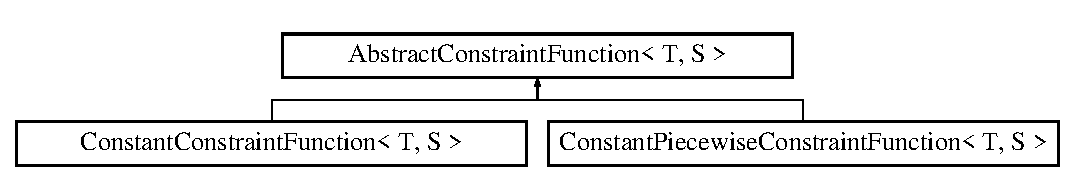
\includegraphics[height=2.000000cm]{dc/d7e/class_abstract_constraint_function}
\end{center}
\end{figure}
\subsection*{Public Member Functions}
\begin{DoxyCompactItemize}
\item 
virtual T {\bfseries get\+Value} (S tree\+Condition)=0\hypertarget{class_abstract_constraint_function_a93beb642087a3dfb45da51a57b3cdbc9}{}\label{class_abstract_constraint_function_a93beb642087a3dfb45da51a57b3cdbc9}

\end{DoxyCompactItemize}


\subsection{Detailed Description}
\subsubsection*{template$<$class T, class S$>$\\*
class Abstract\+Constraint\+Function$<$ T, S $>$}

Abstract class to model tree constraints with different data type 

The documentation for this class was generated from the following file\+:\begin{DoxyCompactItemize}
\item 
constrains/Abstract\+Constraint\+Function.\+h\end{DoxyCompactItemize}

\hypertarget{class_abstract_cost_estimator}{}\section{Abstract\+Cost\+Estimator Class Reference}
\label{class_abstract_cost_estimator}\index{Abstract\+Cost\+Estimator@{Abstract\+Cost\+Estimator}}


{\ttfamily \#include $<$Abstract\+Cost\+Estimator.\+h$>$}

Inheritance diagram for Abstract\+Cost\+Estimator\+:\begin{figure}[H]
\begin{center}
\leavevmode
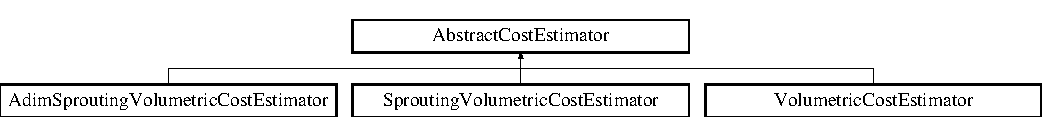
\includegraphics[height=1.568627cm]{db/d7c/class_abstract_cost_estimator}
\end{center}
\end{figure}
\subsection*{Public Member Functions}
\begin{DoxyCompactItemize}
\item 
\hyperlink{class_abstract_cost_estimator_af4ab3e04dbf4c41e10e084e069715973}{Abstract\+Cost\+Estimator} ()
\item 
virtual \hyperlink{class_abstract_cost_estimator_a96e75392a803041183a39eb3bb22b580}{$\sim$\+Abstract\+Cost\+Estimator} ()
\item 
virtual \hyperlink{class_abstract_cost_estimator}{Abstract\+Cost\+Estimator} $\ast$ \hyperlink{class_abstract_cost_estimator_a928e53418b17eb68c443e2a68fe5cbcf}{clone} ()=0
\item 
virtual void \hyperlink{class_abstract_cost_estimator_a8a806c3e4537c6d4acc428b029fd60de}{previous\+State} (\hyperlink{class_abstract_object_c_c_o_tree}{Abstract\+Object\+C\+C\+O\+Tree} $\ast$tree, \hyperlink{class_abstract_vascular_element}{Abstract\+Vascular\+Element} $\ast$parent, \hyperlink{structpoint}{point} i\+New, \hyperlink{structpoint}{point} i\+Test, double d\+Lim)=0
\item 
virtual double \hyperlink{class_abstract_cost_estimator_a2be0c6cc4aa6a73110c75ad903af428e}{compute\+Cost} (\hyperlink{class_abstract_object_c_c_o_tree}{Abstract\+Object\+C\+C\+O\+Tree} $\ast$tree)=0
\end{DoxyCompactItemize}


\subsection{Detailed Description}
Estimates the functional cost of a tree. 

\subsection{Constructor \& Destructor Documentation}
\index{Abstract\+Cost\+Estimator@{Abstract\+Cost\+Estimator}!Abstract\+Cost\+Estimator@{Abstract\+Cost\+Estimator}}
\index{Abstract\+Cost\+Estimator@{Abstract\+Cost\+Estimator}!Abstract\+Cost\+Estimator@{Abstract\+Cost\+Estimator}}
\subsubsection[{\texorpdfstring{Abstract\+Cost\+Estimator()}{AbstractCostEstimator()}}]{\setlength{\rightskip}{0pt plus 5cm}Abstract\+Cost\+Estimator\+::\+Abstract\+Cost\+Estimator (
\begin{DoxyParamCaption}
{}
\end{DoxyParamCaption}
)}\hypertarget{class_abstract_cost_estimator_af4ab3e04dbf4c41e10e084e069715973}{}\label{class_abstract_cost_estimator_af4ab3e04dbf4c41e10e084e069715973}
Common constructor. \index{Abstract\+Cost\+Estimator@{Abstract\+Cost\+Estimator}!````~Abstract\+Cost\+Estimator@{$\sim$\+Abstract\+Cost\+Estimator}}
\index{````~Abstract\+Cost\+Estimator@{$\sim$\+Abstract\+Cost\+Estimator}!Abstract\+Cost\+Estimator@{Abstract\+Cost\+Estimator}}
\subsubsection[{\texorpdfstring{$\sim$\+Abstract\+Cost\+Estimator()}{~AbstractCostEstimator()}}]{\setlength{\rightskip}{0pt plus 5cm}Abstract\+Cost\+Estimator\+::$\sim$\+Abstract\+Cost\+Estimator (
\begin{DoxyParamCaption}
{}
\end{DoxyParamCaption}
)\hspace{0.3cm}{\ttfamily [virtual]}}\hypertarget{class_abstract_cost_estimator_a96e75392a803041183a39eb3bb22b580}{}\label{class_abstract_cost_estimator_a96e75392a803041183a39eb3bb22b580}
Common destructor. 

\subsection{Member Function Documentation}
\index{Abstract\+Cost\+Estimator@{Abstract\+Cost\+Estimator}!clone@{clone}}
\index{clone@{clone}!Abstract\+Cost\+Estimator@{Abstract\+Cost\+Estimator}}
\subsubsection[{\texorpdfstring{clone()=0}{clone()=0}}]{\setlength{\rightskip}{0pt plus 5cm}virtual {\bf Abstract\+Cost\+Estimator}$\ast$ Abstract\+Cost\+Estimator\+::clone (
\begin{DoxyParamCaption}
{}
\end{DoxyParamCaption}
)\hspace{0.3cm}{\ttfamily [pure virtual]}}\hypertarget{class_abstract_cost_estimator_a928e53418b17eb68c443e2a68fe5cbcf}{}\label{class_abstract_cost_estimator_a928e53418b17eb68c443e2a68fe5cbcf}
Clones the current estimator instance. \begin{DoxyReturn}{Returns}
Cloned instance. 
\end{DoxyReturn}


Implemented in \hyperlink{class_adim_sprouting_volumetric_cost_estimator_acc28ad0a4add66222f87d9df84797524}{Adim\+Sprouting\+Volumetric\+Cost\+Estimator}, \hyperlink{class_sprouting_volumetric_cost_estimator_a9adf0950cceb8f82d66639bdabda6043}{Sprouting\+Volumetric\+Cost\+Estimator}, and \hyperlink{class_volumetric_cost_estimator_a513b5fa164962f2761485aebf44072bf}{Volumetric\+Cost\+Estimator}.

\index{Abstract\+Cost\+Estimator@{Abstract\+Cost\+Estimator}!compute\+Cost@{compute\+Cost}}
\index{compute\+Cost@{compute\+Cost}!Abstract\+Cost\+Estimator@{Abstract\+Cost\+Estimator}}
\subsubsection[{\texorpdfstring{compute\+Cost(\+Abstract\+Object\+C\+C\+O\+Tree $\ast$tree)=0}{computeCost(AbstractObjectCCOTree *tree)=0}}]{\setlength{\rightskip}{0pt plus 5cm}virtual double Abstract\+Cost\+Estimator\+::compute\+Cost (
\begin{DoxyParamCaption}
\item[{{\bf Abstract\+Object\+C\+C\+O\+Tree} $\ast$}]{tree}
\end{DoxyParamCaption}
)\hspace{0.3cm}{\ttfamily [pure virtual]}}\hypertarget{class_abstract_cost_estimator_a2be0c6cc4aa6a73110c75ad903af428e}{}\label{class_abstract_cost_estimator_a2be0c6cc4aa6a73110c75ad903af428e}
Computes the functional cost of the given tree. 
\begin{DoxyParams}{Parameters}
{\em root} & Root of the tree at the current step. \\
\hline
\end{DoxyParams}
\begin{DoxyReturn}{Returns}
Cost of the given tree. 
\end{DoxyReturn}


Implemented in \hyperlink{class_adim_sprouting_volumetric_cost_estimator_a14757be74a1c73be8322dab990713936}{Adim\+Sprouting\+Volumetric\+Cost\+Estimator}, \hyperlink{class_sprouting_volumetric_cost_estimator_ab301bfd1c1a93aa0f7535f268499dc63}{Sprouting\+Volumetric\+Cost\+Estimator}, and \hyperlink{class_volumetric_cost_estimator_aca3637b77cc6657e4c5f916f09fd38e3}{Volumetric\+Cost\+Estimator}.

\index{Abstract\+Cost\+Estimator@{Abstract\+Cost\+Estimator}!previous\+State@{previous\+State}}
\index{previous\+State@{previous\+State}!Abstract\+Cost\+Estimator@{Abstract\+Cost\+Estimator}}
\subsubsection[{\texorpdfstring{previous\+State(\+Abstract\+Object\+C\+C\+O\+Tree $\ast$tree, Abstract\+Vascular\+Element $\ast$parent, point i\+New, point i\+Test, double d\+Lim)=0}{previousState(AbstractObjectCCOTree *tree, AbstractVascularElement *parent, point iNew, point iTest, double dLim)=0}}]{\setlength{\rightskip}{0pt plus 5cm}virtual void Abstract\+Cost\+Estimator\+::previous\+State (
\begin{DoxyParamCaption}
\item[{{\bf Abstract\+Object\+C\+C\+O\+Tree} $\ast$}]{tree, }
\item[{{\bf Abstract\+Vascular\+Element} $\ast$}]{parent, }
\item[{{\bf point}}]{i\+New, }
\item[{{\bf point}}]{i\+Test, }
\item[{double}]{d\+Lim}
\end{DoxyParamCaption}
)\hspace{0.3cm}{\ttfamily [pure virtual]}}\hypertarget{class_abstract_cost_estimator_a8a806c3e4537c6d4acc428b029fd60de}{}\label{class_abstract_cost_estimator_a8a806c3e4537c6d4acc428b029fd60de}
Extracts information of the tree at the previous step. 
\begin{DoxyParams}{Parameters}
{\em root} & Root of the tree at the previous step. \\
\hline
{\em parent} & Vascular element where the new vessel will be connected. \\
\hline
{\em i\+New} & Distal position of the new vessel. \\
\hline
{\em i\+Test} & Proximal position of the new vessel. \\
\hline
{\em d\+Lim} & Minimum radius distance from the new vessel to the tree. \\
\hline
\end{DoxyParams}


Implemented in \hyperlink{class_adim_sprouting_volumetric_cost_estimator_aa776aae78d397d422ff6b8041c07c412}{Adim\+Sprouting\+Volumetric\+Cost\+Estimator}, \hyperlink{class_sprouting_volumetric_cost_estimator_a712cbceabb8a8f63521af8d31010f955}{Sprouting\+Volumetric\+Cost\+Estimator}, and \hyperlink{class_volumetric_cost_estimator_a0ff762e6a26e1c6937cc28e88d1dc24d}{Volumetric\+Cost\+Estimator}.



The documentation for this class was generated from the following files\+:\begin{DoxyCompactItemize}
\item 
structures/tree/Abstract\+Cost\+Estimator.\+h\item 
structures/tree/Abstract\+Cost\+Estimator.\+cpp\end{DoxyCompactItemize}

\hypertarget{class_abstract_creator}{}\section{Abstract\+Creator Class Reference}
\label{class_abstract_creator}\index{Abstract\+Creator@{Abstract\+Creator}}
Inheritance diagram for Abstract\+Creator\+:\begin{figure}[H]
\begin{center}
\leavevmode
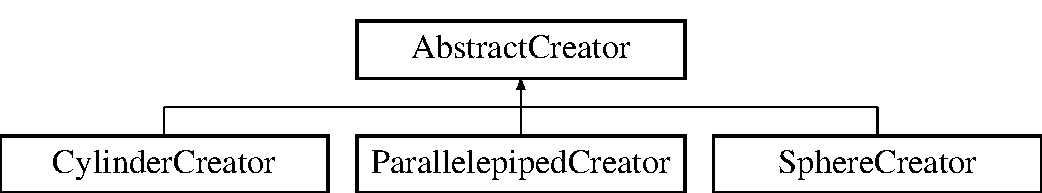
\includegraphics[height=2.000000cm]{class_abstract_creator}
\end{center}
\end{figure}
\subsection*{Public Member Functions}
\begin{DoxyCompactItemize}
\item 
\mbox{\Hypertarget{class_abstract_creator_a1991e446444ffea2b85216b64f2dcf9e}\label{class_abstract_creator_a1991e446444ffea2b85216b64f2dcf9e}} 
virtual void {\bfseries create} (string filename)=0
\end{DoxyCompactItemize}


The documentation for this class was generated from the following files\+:\begin{DoxyCompactItemize}
\item 
creators/Abstract\+Creator.\+h\item 
creators/Abstract\+Creator.\+cpp\end{DoxyCompactItemize}

\hypertarget{class_abstract_domain}{}\section{Abstract\+Domain Class Reference}
\label{class_abstract_domain}\index{Abstract\+Domain@{Abstract\+Domain}}


{\ttfamily \#include $<$Abstract\+Domain.\+h$>$}

Inheritance diagram for Abstract\+Domain\+:\begin{figure}[H]
\begin{center}
\leavevmode
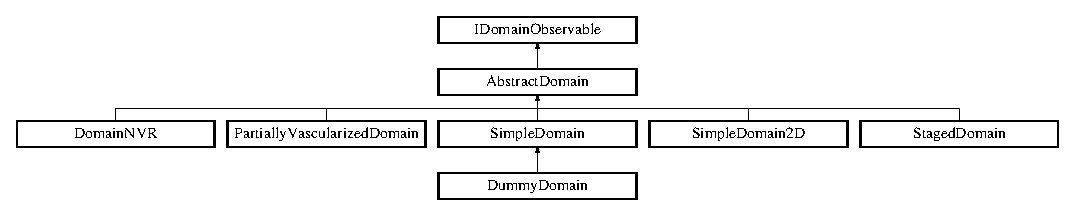
\includegraphics[height=1.857380cm]{d2/d71/class_abstract_domain}
\end{center}
\end{figure}
\subsection*{Public Member Functions}
\begin{DoxyCompactItemize}
\item 
\hyperlink{class_abstract_domain_a18f82b7d0acdb24b3dcdf633510b200c}{Abstract\+Domain} (\hyperlink{class_generator_data}{Generator\+Data} $\ast$\hyperlink{class_abstract_domain_aa37fbabc2bfa92c574f7db7544016b53}{instance\+Data})
\item 
\hyperlink{class_abstract_domain_a145d5a70483d38c157934422da9d99b4}{Abstract\+Domain} (\hyperlink{class_generator_data}{Generator\+Data} $\ast$\hyperlink{class_abstract_domain_aa37fbabc2bfa92c574f7db7544016b53}{instance\+Data}, vector$<$ int $>$ \hyperlink{class_abstract_domain_a765dfd145f6559fc26cc0a36f1bf034a}{growing\+Stages})
\item 
virtual \hyperlink{class_abstract_domain_abad047cac0d8ac7c409864a4e051c67f}{$\sim$\+Abstract\+Domain} ()
\item 
virtual int \hyperlink{class_abstract_domain_a8544eef21fb6700ecc02e9cd50884efd}{is\+Segment\+Inside} (\hyperlink{structpoint}{point} xs, \hyperlink{structpoint}{point} xf)=0
\item 
virtual int \hyperlink{class_abstract_domain_aa151f29002e590832be02829772d38e1}{is\+Valid\+Element} (\hyperlink{class_abstract_vascular_element}{Abstract\+Vascular\+Element} $\ast$element)
\item 
virtual double \hyperlink{class_abstract_domain_a434417bad2396a2ee600932d1d2ded89}{get\+Min\+Bifurcation\+Angle} ()
\item 
virtual void \hyperlink{class_abstract_domain_a0b133239d168c9b70b4997b58d87cca7}{set\+Min\+Bifurcation\+Angle} (double \hyperlink{class_abstract_domain_afa74f9bbc9eb00511fa714ece659e24c}{min\+Angle})
\item 
virtual double \hyperlink{class_abstract_domain_a90ca3dff64bab2428da8ced24e16f4c3}{get\+Characteristic\+Length} ()=0
\item 
virtual double \hyperlink{class_abstract_domain_ac9f39c12182608eb704c051e5d1cbc55}{get\+D\+Lim} (long long int n\+Vessels, double factor)=0
\item 
virtual double $\ast$ \hyperlink{class_abstract_domain_aee2b549d19062b261429f8a442fb4714}{get\+Local\+Neighborhood} (\hyperlink{structpoint}{point} p, long long int n\+Vessels)=0
\item 
virtual double \hyperlink{class_abstract_domain_a049564d82f2c177c39834dfc8da143dc}{get\+Size} ()=0
\item 
virtual \hyperlink{structpoint}{point} \hyperlink{class_abstract_domain_ae31a5b26d1dc628abe24da7a4d375415}{get\+Random\+Point} ()=0
\item 
virtual deque$<$ \hyperlink{structpoint}{point} $>$ \& \hyperlink{class_abstract_domain_a73d2c0e7c670b007bb5dbbdab5ad6b1b}{get\+Random\+Inner\+Points} ()=0
\item 
virtual vtk\+Smart\+Pointer$<$ vtk\+Poly\+Data $>$ \& \hyperlink{class_abstract_domain_abb1e386d2899cb6b725509259a836cd0}{get\+Vtk\+Geometry} ()=0
\item 
long long int \hyperlink{class_abstract_domain_a7d75c8de368f4d97c884b7003cac067c}{get\+Point\+Counter} () const 
\item 
bool \hyperlink{class_abstract_domain_a57291efb709950e97ffd7beb754cd271}{is\+Is\+Convex\+Domain} () const 
\item 
void \hyperlink{class_abstract_domain_a58af16f2954ae8c978c604bf18b99880}{set\+Is\+Convex\+Domain} (bool \hyperlink{class_abstract_domain_acaa76f4d7e102e66b64d10cd652167c9}{is\+Convex\+Domain})
\item 
\hyperlink{class_generator_data}{Generator\+Data} $\ast$ \hyperlink{class_abstract_domain_ad21236a7e37d5dc7763dd0a90d0233ce}{get\+Instance\+Data} ()
\item 
void \hyperlink{class_abstract_domain_a6607101a2ed91199d0675c3d33a029f7}{set\+Instance\+Data} (\hyperlink{class_generator_data}{Generator\+Data} $\ast$\hyperlink{class_abstract_domain_aa37fbabc2bfa92c574f7db7544016b53}{instance\+Data})
\item 
const vector$<$ int $>$ \& {\bfseries get\+Growing\+Stages} () const \hypertarget{class_abstract_domain_af6c54165b4fbb54f22cffac3e6d8376c}{}\label{class_abstract_domain_af6c54165b4fbb54f22cffac3e6d8376c}

\item 
void {\bfseries set\+Growing\+Stages} (const vector$<$ int $>$ \&\hyperlink{class_abstract_domain_a765dfd145f6559fc26cc0a36f1bf034a}{growing\+Stages})\hypertarget{class_abstract_domain_ac2687216bb6c1cbceacb02b5b3265df8}{}\label{class_abstract_domain_ac2687216bb6c1cbceacb02b5b3265df8}

\item 
bool {\bfseries is\+Is\+Bif\+Plane\+Contrained} () const \hypertarget{class_abstract_domain_ac5fd6317f3e6a57a7083d9117a6ebf65}{}\label{class_abstract_domain_ac5fd6317f3e6a57a7083d9117a6ebf65}

\item 
void {\bfseries set\+Is\+Bif\+Plane\+Contrained} (bool \hyperlink{class_abstract_domain_a1b9397f6ac56e1a973d812498153be95}{is\+Bif\+Plane\+Contrained})\hypertarget{class_abstract_domain_ae75192c5000f51e1c6ce53078dd17e03}{}\label{class_abstract_domain_ae75192c5000f51e1c6ce53078dd17e03}

\item 
double {\bfseries get\+Min\+Plane\+Angle} ()\hypertarget{class_abstract_domain_a464979f1f4d9c8445adefdfe3c09c511}{}\label{class_abstract_domain_a464979f1f4d9c8445adefdfe3c09c511}

\item 
void {\bfseries set\+Min\+Plane\+Angle} (double \hyperlink{class_abstract_domain_abf41d751c56a23ba910dd8860d302872}{min\+Plane\+Angle})\hypertarget{class_abstract_domain_a4a92188160489f4799f00955ae1ff523}{}\label{class_abstract_domain_a4a92188160489f4799f00955ae1ff523}

\end{DoxyCompactItemize}
\subsection*{Protected Attributes}
\begin{DoxyCompactItemize}
\item 
vector$<$ int $>$ \hyperlink{class_abstract_domain_a765dfd145f6559fc26cc0a36f1bf034a}{growing\+Stages}
\item 
\hyperlink{class_generator_data}{Generator\+Data} $\ast$ \hyperlink{class_abstract_domain_aa37fbabc2bfa92c574f7db7544016b53}{instance\+Data}
\item 
long long int \hyperlink{class_abstract_domain_af6ca325d56ec51a792d2c0c049e424b0}{point\+Counter}
\item 
bool \hyperlink{class_abstract_domain_acaa76f4d7e102e66b64d10cd652167c9}{is\+Convex\+Domain}
\item 
double \hyperlink{class_abstract_domain_a1cd2c4a6df09d717a7c77c82066f8060}{volume}
\item 
double \hyperlink{class_abstract_domain_afa74f9bbc9eb00511fa714ece659e24c}{min\+Angle}
\item 
bool \hyperlink{class_abstract_domain_a1b9397f6ac56e1a973d812498153be95}{is\+Bif\+Plane\+Contrained}
\item 
double \hyperlink{class_abstract_domain_abf41d751c56a23ba910dd8860d302872}{min\+Plane\+Angle}
\end{DoxyCompactItemize}


\subsection{Detailed Description}
Abstract domain class. Several domain methods guarantee the eficiency during the C\+CO generation, e.\+g., get\+Local\+Neighborhood and get\+D\+Lim, which models the perfusion area of certain terminal in order to establish the minimum length criterion for the new vessel and the local set of vessels where it can be attached to the tree. 

\subsection{Constructor \& Destructor Documentation}
\index{Abstract\+Domain@{Abstract\+Domain}!Abstract\+Domain@{Abstract\+Domain}}
\index{Abstract\+Domain@{Abstract\+Domain}!Abstract\+Domain@{Abstract\+Domain}}
\subsubsection[{\texorpdfstring{Abstract\+Domain(\+Generator\+Data $\ast$instance\+Data)}{AbstractDomain(GeneratorData *instanceData)}}]{\setlength{\rightskip}{0pt plus 5cm}Abstract\+Domain\+::\+Abstract\+Domain (
\begin{DoxyParamCaption}
\item[{{\bf Generator\+Data} $\ast$}]{instance\+Data}
\end{DoxyParamCaption}
)}\hypertarget{class_abstract_domain_a18f82b7d0acdb24b3dcdf633510b200c}{}\label{class_abstract_domain_a18f82b7d0acdb24b3dcdf633510b200c}
Constructor. 
\begin{DoxyParams}{Parameters}
{\em instance\+Data} & Wrapper with parameters associated to a tree generation process. \\
\hline
\end{DoxyParams}
\index{Abstract\+Domain@{Abstract\+Domain}!Abstract\+Domain@{Abstract\+Domain}}
\index{Abstract\+Domain@{Abstract\+Domain}!Abstract\+Domain@{Abstract\+Domain}}
\subsubsection[{\texorpdfstring{Abstract\+Domain(\+Generator\+Data $\ast$instance\+Data, vector$<$ int $>$ growing\+Stages)}{AbstractDomain(GeneratorData *instanceData, vector< int > growingStages)}}]{\setlength{\rightskip}{0pt plus 5cm}Abstract\+Domain\+::\+Abstract\+Domain (
\begin{DoxyParamCaption}
\item[{{\bf Generator\+Data} $\ast$}]{instance\+Data, }
\item[{vector$<$ int $>$}]{growing\+Stages}
\end{DoxyParamCaption}
)}\hypertarget{class_abstract_domain_a145d5a70483d38c157934422da9d99b4}{}\label{class_abstract_domain_a145d5a70483d38c157934422da9d99b4}
Constructor. 
\begin{DoxyParams}{Parameters}
{\em instance\+Data} & Wrapper with parameters associated to a tree generation process. \\
\hline
{\em growing\+Stages} & Stages allowed to grow. \\
\hline
\end{DoxyParams}
\index{Abstract\+Domain@{Abstract\+Domain}!````~Abstract\+Domain@{$\sim$\+Abstract\+Domain}}
\index{````~Abstract\+Domain@{$\sim$\+Abstract\+Domain}!Abstract\+Domain@{Abstract\+Domain}}
\subsubsection[{\texorpdfstring{$\sim$\+Abstract\+Domain()}{~AbstractDomain()}}]{\setlength{\rightskip}{0pt plus 5cm}Abstract\+Domain\+::$\sim$\+Abstract\+Domain (
\begin{DoxyParamCaption}
{}
\end{DoxyParamCaption}
)\hspace{0.3cm}{\ttfamily [virtual]}}\hypertarget{class_abstract_domain_abad047cac0d8ac7c409864a4e051c67f}{}\label{class_abstract_domain_abad047cac0d8ac7c409864a4e051c67f}
Destructor. 

\subsection{Member Function Documentation}
\index{Abstract\+Domain@{Abstract\+Domain}!get\+Characteristic\+Length@{get\+Characteristic\+Length}}
\index{get\+Characteristic\+Length@{get\+Characteristic\+Length}!Abstract\+Domain@{Abstract\+Domain}}
\subsubsection[{\texorpdfstring{get\+Characteristic\+Length()=0}{getCharacteristicLength()=0}}]{\setlength{\rightskip}{0pt plus 5cm}virtual double Abstract\+Domain\+::get\+Characteristic\+Length (
\begin{DoxyParamCaption}
{}
\end{DoxyParamCaption}
)\hspace{0.3cm}{\ttfamily [pure virtual]}}\hypertarget{class_abstract_domain_a90ca3dff64bab2428da8ced24e16f4c3}{}\label{class_abstract_domain_a90ca3dff64bab2428da8ced24e16f4c3}
Estimates a characteristic length for the current domain. This length is useful to estimate the perfusion volume of the domain. \begin{DoxyReturn}{Returns}
Chracteristic length. 
\end{DoxyReturn}


Implemented in \hyperlink{class_partially_vascularized_domain_a1ec0827e05801a1a3219cbd4e87ac64c}{Partially\+Vascularized\+Domain}, \hyperlink{class_domain_n_v_r_a590ea752ce83767038de90138faf8a21}{Domain\+N\+VR}, \hyperlink{class_simple_domain_a2a7e2919f633368b85aa3e9cfd0e57ab}{Simple\+Domain}, \hyperlink{class_intersection_vascularized_domain_a6ded581a637a098d2ddfec6ae6801132}{Intersection\+Vascularized\+Domain}, \hyperlink{class_simple_domain2_d_a5bf4df64fe80dae1e394b2f2c73c3d05}{Simple\+Domain2D}, and \hyperlink{class_staged_domain_aec389e04bcd549140b29dbc9c56cf29b}{Staged\+Domain}.

\index{Abstract\+Domain@{Abstract\+Domain}!get\+D\+Lim@{get\+D\+Lim}}
\index{get\+D\+Lim@{get\+D\+Lim}!Abstract\+Domain@{Abstract\+Domain}}
\subsubsection[{\texorpdfstring{get\+D\+Lim(long long int n\+Vessels, double factor)=0}{getDLim(long long int nVessels, double factor)=0}}]{\setlength{\rightskip}{0pt plus 5cm}virtual double Abstract\+Domain\+::get\+D\+Lim (
\begin{DoxyParamCaption}
\item[{long long int}]{n\+Vessels, }
\item[{double}]{factor}
\end{DoxyParamCaption}
)\hspace{0.3cm}{\ttfamily [pure virtual]}}\hypertarget{class_abstract_domain_ac9f39c12182608eb704c051e5d1cbc55}{}\label{class_abstract_domain_ac9f39c12182608eb704c051e5d1cbc55}
Minimum distance between a new vessel terminal and the tree based on the current terminal perfusion. This is lower bound criteria for the vessel length and also aids toward a spatially homogeneous terminal distribution. 
\begin{DoxyParams}{Parameters}
{\em n\+Vessels} & Quantity of terminals in the current tree. \\
\hline
{\em factor} & Factor used to scale a perfusion measure in order to estimate the D\+Lim value. \\
\hline
\end{DoxyParams}
\begin{DoxyReturn}{Returns}
D\+Lim value. 
\end{DoxyReturn}


Implemented in \hyperlink{class_partially_vascularized_domain_a7cfa7a304d236b933311f8ac5149662e}{Partially\+Vascularized\+Domain}, \hyperlink{class_domain_n_v_r_a5e67e5367a9f22ab0243e06d92abccab}{Domain\+N\+VR}, \hyperlink{class_simple_domain_a413c188add5702b18bb838283b68bcbe}{Simple\+Domain}, \hyperlink{class_intersection_vascularized_domain_a24e31c45b099a27ea3d13b1923ea5340}{Intersection\+Vascularized\+Domain}, \hyperlink{class_simple_domain2_d_a60dbee1351f604d7ee61121d923de823}{Simple\+Domain2D}, and \hyperlink{class_staged_domain_a4bb50d4e92dc81e0c87aa0b4190138b3}{Staged\+Domain}.

\index{Abstract\+Domain@{Abstract\+Domain}!get\+Instance\+Data@{get\+Instance\+Data}}
\index{get\+Instance\+Data@{get\+Instance\+Data}!Abstract\+Domain@{Abstract\+Domain}}
\subsubsection[{\texorpdfstring{get\+Instance\+Data()}{getInstanceData()}}]{\setlength{\rightskip}{0pt plus 5cm}{\bf Generator\+Data} $\ast$ Abstract\+Domain\+::get\+Instance\+Data (
\begin{DoxyParamCaption}
{}
\end{DoxyParamCaption}
)}\hypertarget{class_abstract_domain_ad21236a7e37d5dc7763dd0a90d0233ce}{}\label{class_abstract_domain_ad21236a7e37d5dc7763dd0a90d0233ce}
Default getter of {\ttfamily instance\+Data}. \begin{DoxyReturn}{Returns}
{\ttfamily instance\+Data} 
\end{DoxyReturn}
\index{Abstract\+Domain@{Abstract\+Domain}!get\+Local\+Neighborhood@{get\+Local\+Neighborhood}}
\index{get\+Local\+Neighborhood@{get\+Local\+Neighborhood}!Abstract\+Domain@{Abstract\+Domain}}
\subsubsection[{\texorpdfstring{get\+Local\+Neighborhood(point p, long long int n\+Vessels)=0}{getLocalNeighborhood(point p, long long int nVessels)=0}}]{\setlength{\rightskip}{0pt plus 5cm}virtual double$\ast$ Abstract\+Domain\+::get\+Local\+Neighborhood (
\begin{DoxyParamCaption}
\item[{{\bf point}}]{p, }
\item[{long long int}]{n\+Vessels}
\end{DoxyParamCaption}
)\hspace{0.3cm}{\ttfamily [pure virtual]}}\hypertarget{class_abstract_domain_aee2b549d19062b261429f8a442fb4714}{}\label{class_abstract_domain_aee2b549d19062b261429f8a442fb4714}
Returns the local neighbors to the {\ttfamily p} point locus. The amount of neighbors is estimated based on the current terminal perfusion. 
\begin{DoxyParams}{Parameters}
{\em p} & Central point of the neighborhood. \\
\hline
{\em n\+Vessels} & Amount of terminals in the tree. \\
\hline
\end{DoxyParams}
\begin{DoxyReturn}{Returns}
Array of neighbor vessels. 
\end{DoxyReturn}


Implemented in \hyperlink{class_partially_vascularized_domain_a379893eff3b1612932f4689a478e73ee}{Partially\+Vascularized\+Domain}, \hyperlink{class_domain_n_v_r_a5d97b6894250d8034c5e0679266f9fb1}{Domain\+N\+VR}, \hyperlink{class_simple_domain_a0491a8bc37f8e27031f2b67b79eaf45e}{Simple\+Domain}, \hyperlink{class_intersection_vascularized_domain_a4b35793edb3ec9847e8be75d81dfbd9d}{Intersection\+Vascularized\+Domain}, \hyperlink{class_simple_domain2_d_a5c7eaa0e32e25950149c4735bd02c671}{Simple\+Domain2D}, and \hyperlink{class_staged_domain_ad8107b681fcba3794ea4cd9b1a5a2edd}{Staged\+Domain}.

\index{Abstract\+Domain@{Abstract\+Domain}!get\+Min\+Bifurcation\+Angle@{get\+Min\+Bifurcation\+Angle}}
\index{get\+Min\+Bifurcation\+Angle@{get\+Min\+Bifurcation\+Angle}!Abstract\+Domain@{Abstract\+Domain}}
\subsubsection[{\texorpdfstring{get\+Min\+Bifurcation\+Angle()}{getMinBifurcationAngle()}}]{\setlength{\rightskip}{0pt plus 5cm}double Abstract\+Domain\+::get\+Min\+Bifurcation\+Angle (
\begin{DoxyParamCaption}
{}
\end{DoxyParamCaption}
)\hspace{0.3cm}{\ttfamily [virtual]}}\hypertarget{class_abstract_domain_a434417bad2396a2ee600932d1d2ded89}{}\label{class_abstract_domain_a434417bad2396a2ee600932d1d2ded89}
Returns the maximum opening angle that the hosted tree can generate. \begin{DoxyReturn}{Returns}
Maximum bifurcation angle for vessels generated inside this domain. 
\end{DoxyReturn}


Reimplemented in \hyperlink{class_staged_domain_a139146506055f007980898b55fc894e0}{Staged\+Domain}.

\index{Abstract\+Domain@{Abstract\+Domain}!get\+Point\+Counter@{get\+Point\+Counter}}
\index{get\+Point\+Counter@{get\+Point\+Counter}!Abstract\+Domain@{Abstract\+Domain}}
\subsubsection[{\texorpdfstring{get\+Point\+Counter() const }{getPointCounter() const }}]{\setlength{\rightskip}{0pt plus 5cm}long long int Abstract\+Domain\+::get\+Point\+Counter (
\begin{DoxyParamCaption}
{}
\end{DoxyParamCaption}
) const}\hypertarget{class_abstract_domain_a7d75c8de368f4d97c884b7003cac067c}{}\label{class_abstract_domain_a7d75c8de368f4d97c884b7003cac067c}
Returns the quantity of points that have been consumed. \begin{DoxyReturn}{Returns}
Quantity of points consumed. 
\end{DoxyReturn}
\index{Abstract\+Domain@{Abstract\+Domain}!get\+Random\+Inner\+Points@{get\+Random\+Inner\+Points}}
\index{get\+Random\+Inner\+Points@{get\+Random\+Inner\+Points}!Abstract\+Domain@{Abstract\+Domain}}
\subsubsection[{\texorpdfstring{get\+Random\+Inner\+Points()=0}{getRandomInnerPoints()=0}}]{\setlength{\rightskip}{0pt plus 5cm}virtual deque$<${\bf point}$>$\& Abstract\+Domain\+::get\+Random\+Inner\+Points (
\begin{DoxyParamCaption}
{}
\end{DoxyParamCaption}
)\hspace{0.3cm}{\ttfamily [pure virtual]}}\hypertarget{class_abstract_domain_a73d2c0e7c670b007bb5dbbdab5ad6b1b}{}\label{class_abstract_domain_a73d2c0e7c670b007bb5dbbdab5ad6b1b}
Return a set of inner domain points. \begin{DoxyReturn}{Returns}
Set of inner domain points. 
\end{DoxyReturn}


Implemented in \hyperlink{class_partially_vascularized_domain_abbfb8f486b00e62117b564874a454395}{Partially\+Vascularized\+Domain}, \hyperlink{class_domain_n_v_r_a2b303bccf9a1db72e3bae866d7947f2d}{Domain\+N\+VR}, \hyperlink{class_simple_domain_acfe3e4aeaea246579b6102707d050bf0}{Simple\+Domain}, \hyperlink{class_intersection_vascularized_domain_afa0103c0c3ed989e1b67e50d14684321}{Intersection\+Vascularized\+Domain}, \hyperlink{class_simple_domain2_d_a08eddf131c1ed43cf7cc34e347fd372f}{Simple\+Domain2D}, and \hyperlink{class_staged_domain_a5a5398712e064cbd706f701c8294bbad}{Staged\+Domain}.

\index{Abstract\+Domain@{Abstract\+Domain}!get\+Random\+Point@{get\+Random\+Point}}
\index{get\+Random\+Point@{get\+Random\+Point}!Abstract\+Domain@{Abstract\+Domain}}
\subsubsection[{\texorpdfstring{get\+Random\+Point()=0}{getRandomPoint()=0}}]{\setlength{\rightskip}{0pt plus 5cm}virtual {\bf point} Abstract\+Domain\+::get\+Random\+Point (
\begin{DoxyParamCaption}
{}
\end{DoxyParamCaption}
)\hspace{0.3cm}{\ttfamily [pure virtual]}}\hypertarget{class_abstract_domain_ae31a5b26d1dc628abe24da7a4d375415}{}\label{class_abstract_domain_ae31a5b26d1dc628abe24da7a4d375415}
Return a random point inside the domain. \begin{DoxyReturn}{Returns}
Point inside the domain. 
\end{DoxyReturn}


Implemented in \hyperlink{class_partially_vascularized_domain_a817dcd8122892b14ed112135aa4a1fe0}{Partially\+Vascularized\+Domain}, \hyperlink{class_domain_n_v_r_a88c76433bc3e8a1c1d60d4e7643f46d0}{Domain\+N\+VR}, \hyperlink{class_simple_domain_afcf98b009584217d8ab03e0dbfa86839}{Simple\+Domain}, \hyperlink{class_intersection_vascularized_domain_a39e0fd3443fed3fecf4ecc799e39baa2}{Intersection\+Vascularized\+Domain}, \hyperlink{class_staged_domain_a90178baeab98fe08850977e7924c2780}{Staged\+Domain}, \hyperlink{class_simple_domain2_d_a8b19e2fa69a0f13813b0296f270f11e9}{Simple\+Domain2D}, and \hyperlink{class_dummy_domain_a72074e5e3e53028ec4b73bffee1ba229}{Dummy\+Domain}.

\index{Abstract\+Domain@{Abstract\+Domain}!get\+Size@{get\+Size}}
\index{get\+Size@{get\+Size}!Abstract\+Domain@{Abstract\+Domain}}
\subsubsection[{\texorpdfstring{get\+Size()=0}{getSize()=0}}]{\setlength{\rightskip}{0pt plus 5cm}virtual double Abstract\+Domain\+::get\+Size (
\begin{DoxyParamCaption}
{}
\end{DoxyParamCaption}
)\hspace{0.3cm}{\ttfamily [pure virtual]}}\hypertarget{class_abstract_domain_a049564d82f2c177c39834dfc8da143dc}{}\label{class_abstract_domain_a049564d82f2c177c39834dfc8da143dc}
Computes the size of the domain. \begin{DoxyReturn}{Returns}
Size of the domain. 
\end{DoxyReturn}


Implemented in \hyperlink{class_partially_vascularized_domain_a88c04b73a8ffd9e8ddbc4a1c118a1795}{Partially\+Vascularized\+Domain}, \hyperlink{class_domain_n_v_r_aae7b6782c1caab8cf5246c802be410cc}{Domain\+N\+VR}, \hyperlink{class_simple_domain_a0a05345c81234a3e616447a16e9150c0}{Simple\+Domain}, \hyperlink{class_intersection_vascularized_domain_a4c4dc6ce4711752e7d082346499d70b5}{Intersection\+Vascularized\+Domain}, \hyperlink{class_staged_domain_a807d7b1c56b5a6ccce593513baebf3b1}{Staged\+Domain}, and \hyperlink{class_simple_domain2_d_ad5e1ba1529fd8088f64af603cc5c18a3}{Simple\+Domain2D}.

\index{Abstract\+Domain@{Abstract\+Domain}!get\+Vtk\+Geometry@{get\+Vtk\+Geometry}}
\index{get\+Vtk\+Geometry@{get\+Vtk\+Geometry}!Abstract\+Domain@{Abstract\+Domain}}
\subsubsection[{\texorpdfstring{get\+Vtk\+Geometry()=0}{getVtkGeometry()=0}}]{\setlength{\rightskip}{0pt plus 5cm}virtual vtk\+Smart\+Pointer$<$vtk\+Poly\+Data$>$\& Abstract\+Domain\+::get\+Vtk\+Geometry (
\begin{DoxyParamCaption}
{}
\end{DoxyParamCaption}
)\hspace{0.3cm}{\ttfamily [pure virtual]}}\hypertarget{class_abstract_domain_abb1e386d2899cb6b725509259a836cd0}{}\label{class_abstract_domain_abb1e386d2899cb6b725509259a836cd0}
Returns the vtk\+Polydata with the domain representation. \begin{DoxyReturn}{Returns}
vtk\+Polydata with the domain representation. 
\end{DoxyReturn}


Implemented in \hyperlink{class_partially_vascularized_domain_aa2acdedb98eb9cd168b9ab4cfa38c485}{Partially\+Vascularized\+Domain}, \hyperlink{class_domain_n_v_r_a50591c2d4b9e055821cc53416bf4263c}{Domain\+N\+VR}, \hyperlink{class_simple_domain_a13f9ab047e641a022648ca6468651f9f}{Simple\+Domain}, \hyperlink{class_intersection_vascularized_domain_aacdc4a4263423e8c8dd992ba4f00f826}{Intersection\+Vascularized\+Domain}, \hyperlink{class_simple_domain2_d_a0c4505e70d9530586bcb0ab943bb9a9a}{Simple\+Domain2D}, and \hyperlink{class_staged_domain_a69530fd545f217410433367a7e219fbf}{Staged\+Domain}.

\index{Abstract\+Domain@{Abstract\+Domain}!is\+Is\+Convex\+Domain@{is\+Is\+Convex\+Domain}}
\index{is\+Is\+Convex\+Domain@{is\+Is\+Convex\+Domain}!Abstract\+Domain@{Abstract\+Domain}}
\subsubsection[{\texorpdfstring{is\+Is\+Convex\+Domain() const }{isIsConvexDomain() const }}]{\setlength{\rightskip}{0pt plus 5cm}bool Abstract\+Domain\+::is\+Is\+Convex\+Domain (
\begin{DoxyParamCaption}
{}
\end{DoxyParamCaption}
) const}\hypertarget{class_abstract_domain_a57291efb709950e97ffd7beb754cd271}{}\label{class_abstract_domain_a57291efb709950e97ffd7beb754cd271}
Getter for {\ttfamily is\+Convex\+Domain} variable. \begin{DoxyReturn}{Returns}
Returns if the domain is setted as convex. 
\end{DoxyReturn}
\index{Abstract\+Domain@{Abstract\+Domain}!is\+Segment\+Inside@{is\+Segment\+Inside}}
\index{is\+Segment\+Inside@{is\+Segment\+Inside}!Abstract\+Domain@{Abstract\+Domain}}
\subsubsection[{\texorpdfstring{is\+Segment\+Inside(point xs, point xf)=0}{isSegmentInside(point xs, point xf)=0}}]{\setlength{\rightskip}{0pt plus 5cm}virtual int Abstract\+Domain\+::is\+Segment\+Inside (
\begin{DoxyParamCaption}
\item[{{\bf point}}]{xs, }
\item[{{\bf point}}]{xf}
\end{DoxyParamCaption}
)\hspace{0.3cm}{\ttfamily [pure virtual]}}\hypertarget{class_abstract_domain_a8544eef21fb6700ecc02e9cd50884efd}{}\label{class_abstract_domain_a8544eef21fb6700ecc02e9cd50884efd}
Returns if the segment defined by the vertexes {\ttfamily xs} and {\ttfamily xf} is inside the current domain. 
\begin{DoxyParams}{Parameters}
{\em xs} & Start point of the segment. \\
\hline
{\em xf} & End point of the segment. \\
\hline
\end{DoxyParams}
\begin{DoxyReturn}{Returns}
1 if the segment defined by the vertexes {\ttfamily xs} and {\ttfamily xf} is inside the current domain otherwise 0. 
\end{DoxyReturn}


Implemented in \hyperlink{class_partially_vascularized_domain_a485e0e573369f76ef59477fc5ac8ea9b}{Partially\+Vascularized\+Domain}, \hyperlink{class_domain_n_v_r_a46b7a56ffdb8f8e0cfcd2a5761571394}{Domain\+N\+VR}, \hyperlink{class_simple_domain_ab1e60afe4302149098b11631d20aebb7}{Simple\+Domain}, \hyperlink{class_intersection_vascularized_domain_accd160eb77fede65322d67293177e54f}{Intersection\+Vascularized\+Domain}, \hyperlink{class_simple_domain2_d_a18706cdbe4f61a71eceb7257fd4ec6dd}{Simple\+Domain2D}, and \hyperlink{class_staged_domain_a2f13523c9e014efd270df926aabdbc76}{Staged\+Domain}.

\index{Abstract\+Domain@{Abstract\+Domain}!is\+Valid\+Element@{is\+Valid\+Element}}
\index{is\+Valid\+Element@{is\+Valid\+Element}!Abstract\+Domain@{Abstract\+Domain}}
\subsubsection[{\texorpdfstring{is\+Valid\+Element(\+Abstract\+Vascular\+Element $\ast$element)}{isValidElement(AbstractVascularElement *element)}}]{\setlength{\rightskip}{0pt plus 5cm}int Abstract\+Domain\+::is\+Valid\+Element (
\begin{DoxyParamCaption}
\item[{{\bf Abstract\+Vascular\+Element} $\ast$}]{element}
\end{DoxyParamCaption}
)\hspace{0.3cm}{\ttfamily [virtual]}}\hypertarget{class_abstract_domain_aa151f29002e590832be02829772d38e1}{}\label{class_abstract_domain_aa151f29002e590832be02829772d38e1}
Returns if the vascular element is eligible to be a parent vessel. 
\begin{DoxyParams}{Parameters}
{\em element} & Vascular element. \\
\hline
\end{DoxyParams}
\begin{DoxyReturn}{Returns}
1 if it is eligible. 
\end{DoxyReturn}


Reimplemented in \hyperlink{class_staged_domain_a083dae621ca3d910b23f5cd85ba23d65}{Staged\+Domain}.

\index{Abstract\+Domain@{Abstract\+Domain}!set\+Instance\+Data@{set\+Instance\+Data}}
\index{set\+Instance\+Data@{set\+Instance\+Data}!Abstract\+Domain@{Abstract\+Domain}}
\subsubsection[{\texorpdfstring{set\+Instance\+Data(\+Generator\+Data $\ast$instance\+Data)}{setInstanceData(GeneratorData *instanceData)}}]{\setlength{\rightskip}{0pt plus 5cm}void Abstract\+Domain\+::set\+Instance\+Data (
\begin{DoxyParamCaption}
\item[{{\bf Generator\+Data} $\ast$}]{instance\+Data}
\end{DoxyParamCaption}
)}\hypertarget{class_abstract_domain_a6607101a2ed91199d0675c3d33a029f7}{}\label{class_abstract_domain_a6607101a2ed91199d0675c3d33a029f7}
Default setter of {\ttfamily instance\+Data}. 
\begin{DoxyParams}{Parameters}
{\em instance\+Data} & Instance for {\ttfamily instance\+Data}. \\
\hline
\end{DoxyParams}
\index{Abstract\+Domain@{Abstract\+Domain}!set\+Is\+Convex\+Domain@{set\+Is\+Convex\+Domain}}
\index{set\+Is\+Convex\+Domain@{set\+Is\+Convex\+Domain}!Abstract\+Domain@{Abstract\+Domain}}
\subsubsection[{\texorpdfstring{set\+Is\+Convex\+Domain(bool is\+Convex\+Domain)}{setIsConvexDomain(bool isConvexDomain)}}]{\setlength{\rightskip}{0pt plus 5cm}void Abstract\+Domain\+::set\+Is\+Convex\+Domain (
\begin{DoxyParamCaption}
\item[{bool}]{is\+Convex\+Domain}
\end{DoxyParamCaption}
)}\hypertarget{class_abstract_domain_a58af16f2954ae8c978c604bf18b99880}{}\label{class_abstract_domain_a58af16f2954ae8c978c604bf18b99880}
Setter for {\ttfamily is\+Convex\+Domain} variable. 
\begin{DoxyParams}{Parameters}
{\em is\+Convex\+Domain} & Sets the domain as convex or non-\/convex. \\
\hline
\end{DoxyParams}
\index{Abstract\+Domain@{Abstract\+Domain}!set\+Min\+Bifurcation\+Angle@{set\+Min\+Bifurcation\+Angle}}
\index{set\+Min\+Bifurcation\+Angle@{set\+Min\+Bifurcation\+Angle}!Abstract\+Domain@{Abstract\+Domain}}
\subsubsection[{\texorpdfstring{set\+Min\+Bifurcation\+Angle(double min\+Angle)}{setMinBifurcationAngle(double minAngle)}}]{\setlength{\rightskip}{0pt plus 5cm}void Abstract\+Domain\+::set\+Min\+Bifurcation\+Angle (
\begin{DoxyParamCaption}
\item[{double}]{min\+Angle}
\end{DoxyParamCaption}
)\hspace{0.3cm}{\ttfamily [virtual]}}\hypertarget{class_abstract_domain_a0b133239d168c9b70b4997b58d87cca7}{}\label{class_abstract_domain_a0b133239d168c9b70b4997b58d87cca7}
Sets the maximum opening angle that the hosted tree can generate. 
\begin{DoxyParams}{Parameters}
{\em min\+Angle} & Maximum bifurcation angle for vessels generated inside this domain. \\
\hline
\end{DoxyParams}


\subsection{Member Data Documentation}
\index{Abstract\+Domain@{Abstract\+Domain}!growing\+Stages@{growing\+Stages}}
\index{growing\+Stages@{growing\+Stages}!Abstract\+Domain@{Abstract\+Domain}}
\subsubsection[{\texorpdfstring{growing\+Stages}{growingStages}}]{\setlength{\rightskip}{0pt plus 5cm}vector$<$int$>$ Abstract\+Domain\+::growing\+Stages\hspace{0.3cm}{\ttfamily [protected]}}\hypertarget{class_abstract_domain_a765dfd145f6559fc26cc0a36f1bf034a}{}\label{class_abstract_domain_a765dfd145f6559fc26cc0a36f1bf034a}
Vessels with stages contained in such list are allowed to grow. If empty, all vessels are allowed to grow. \index{Abstract\+Domain@{Abstract\+Domain}!instance\+Data@{instance\+Data}}
\index{instance\+Data@{instance\+Data}!Abstract\+Domain@{Abstract\+Domain}}
\subsubsection[{\texorpdfstring{instance\+Data}{instanceData}}]{\setlength{\rightskip}{0pt plus 5cm}{\bf Generator\+Data}$\ast$ Abstract\+Domain\+::instance\+Data\hspace{0.3cm}{\ttfamily [protected]}}\hypertarget{class_abstract_domain_aa37fbabc2bfa92c574f7db7544016b53}{}\label{class_abstract_domain_aa37fbabc2bfa92c574f7db7544016b53}
Wrapper with parameters associated to a tree generation process. \index{Abstract\+Domain@{Abstract\+Domain}!is\+Bif\+Plane\+Contrained@{is\+Bif\+Plane\+Contrained}}
\index{is\+Bif\+Plane\+Contrained@{is\+Bif\+Plane\+Contrained}!Abstract\+Domain@{Abstract\+Domain}}
\subsubsection[{\texorpdfstring{is\+Bif\+Plane\+Contrained}{isBifPlaneContrained}}]{\setlength{\rightskip}{0pt plus 5cm}bool Abstract\+Domain\+::is\+Bif\+Plane\+Contrained\hspace{0.3cm}{\ttfamily [protected]}}\hypertarget{class_abstract_domain_a1b9397f6ac56e1a973d812498153be95}{}\label{class_abstract_domain_a1b9397f6ac56e1a973d812498153be95}
Boolean value that models if the domain present any restriction regarding the opening angle between the bifurcation plane and a new daughter vessel. \index{Abstract\+Domain@{Abstract\+Domain}!is\+Convex\+Domain@{is\+Convex\+Domain}}
\index{is\+Convex\+Domain@{is\+Convex\+Domain}!Abstract\+Domain@{Abstract\+Domain}}
\subsubsection[{\texorpdfstring{is\+Convex\+Domain}{isConvexDomain}}]{\setlength{\rightskip}{0pt plus 5cm}bool Abstract\+Domain\+::is\+Convex\+Domain\hspace{0.3cm}{\ttfamily [protected]}}\hypertarget{class_abstract_domain_acaa76f4d7e102e66b64d10cd652167c9}{}\label{class_abstract_domain_acaa76f4d7e102e66b64d10cd652167c9}
Boolean value that models if the domain is convex or not. For convex domain some optimizations are applied. \index{Abstract\+Domain@{Abstract\+Domain}!min\+Angle@{min\+Angle}}
\index{min\+Angle@{min\+Angle}!Abstract\+Domain@{Abstract\+Domain}}
\subsubsection[{\texorpdfstring{min\+Angle}{minAngle}}]{\setlength{\rightskip}{0pt plus 5cm}double Abstract\+Domain\+::min\+Angle\hspace{0.3cm}{\ttfamily [protected]}}\hypertarget{class_abstract_domain_afa74f9bbc9eb00511fa714ece659e24c}{}\label{class_abstract_domain_afa74f9bbc9eb00511fa714ece659e24c}
Minimum bifurcation angle for vessels generated inside this domain \index{Abstract\+Domain@{Abstract\+Domain}!min\+Plane\+Angle@{min\+Plane\+Angle}}
\index{min\+Plane\+Angle@{min\+Plane\+Angle}!Abstract\+Domain@{Abstract\+Domain}}
\subsubsection[{\texorpdfstring{min\+Plane\+Angle}{minPlaneAngle}}]{\setlength{\rightskip}{0pt plus 5cm}double Abstract\+Domain\+::min\+Plane\+Angle\hspace{0.3cm}{\ttfamily [protected]}}\hypertarget{class_abstract_domain_abf41d751c56a23ba910dd8860d302872}{}\label{class_abstract_domain_abf41d751c56a23ba910dd8860d302872}
Minimum angle between the bifurcation plane and a new daughter vessel. \index{Abstract\+Domain@{Abstract\+Domain}!point\+Counter@{point\+Counter}}
\index{point\+Counter@{point\+Counter}!Abstract\+Domain@{Abstract\+Domain}}
\subsubsection[{\texorpdfstring{point\+Counter}{pointCounter}}]{\setlength{\rightskip}{0pt plus 5cm}long long int Abstract\+Domain\+::point\+Counter\hspace{0.3cm}{\ttfamily [protected]}}\hypertarget{class_abstract_domain_af6ca325d56ec51a792d2c0c049e424b0}{}\label{class_abstract_domain_af6ca325d56ec51a792d2c0c049e424b0}
Quantity of points that have been consumed. \index{Abstract\+Domain@{Abstract\+Domain}!volume@{volume}}
\index{volume@{volume}!Abstract\+Domain@{Abstract\+Domain}}
\subsubsection[{\texorpdfstring{volume}{volume}}]{\setlength{\rightskip}{0pt plus 5cm}double Abstract\+Domain\+::volume\hspace{0.3cm}{\ttfamily [protected]}}\hypertarget{class_abstract_domain_a1cd2c4a6df09d717a7c77c82066f8060}{}\label{class_abstract_domain_a1cd2c4a6df09d717a7c77c82066f8060}
Vascular volume. 

The documentation for this class was generated from the following files\+:\begin{DoxyCompactItemize}
\item 
structures/domain/Abstract\+Domain.\+h\item 
structures/domain/Abstract\+Domain.\+cpp\end{DoxyCompactItemize}

\hypertarget{class_abstract_object_c_c_o_tree}{}\section{Abstract\+Object\+C\+C\+O\+Tree Class Reference}
\label{class_abstract_object_c_c_o_tree}\index{Abstract\+Object\+C\+C\+O\+Tree@{Abstract\+Object\+C\+C\+O\+Tree}}


{\ttfamily \#include $<$Abstract\+Object\+C\+C\+O\+Tree.\+h$>$}

Inheritance diagram for Abstract\+Object\+C\+C\+O\+Tree\+:\begin{figure}[H]
\begin{center}
\leavevmode
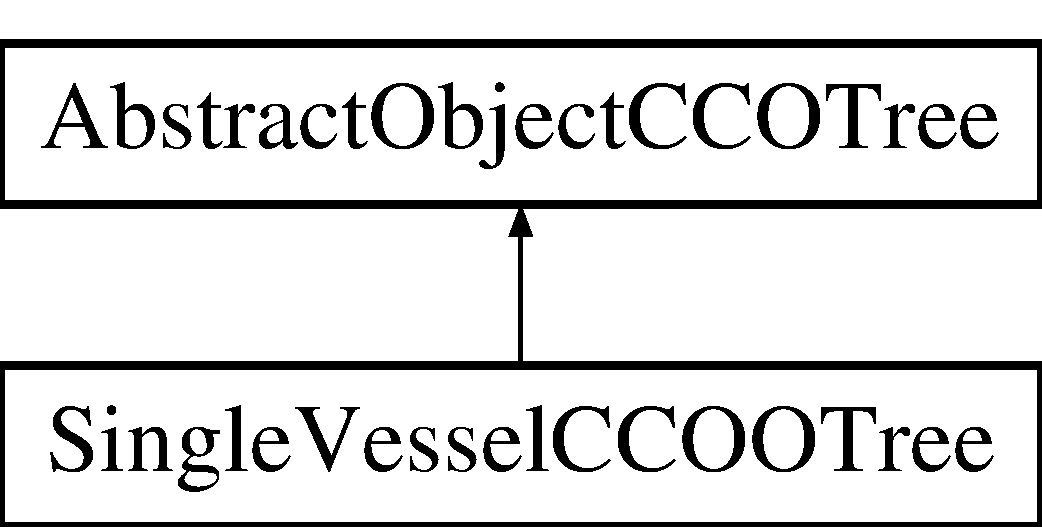
\includegraphics[height=2.000000cm]{d5/df4/class_abstract_object_c_c_o_tree}
\end{center}
\end{figure}
\subsection*{Public Member Functions}
\begin{DoxyCompactItemize}
\item 
\hyperlink{class_abstract_object_c_c_o_tree_ac6be6b54f61f0db2dc79f47c4d1a1a3c}{Abstract\+Object\+C\+C\+O\+Tree} (\hyperlink{class_generator_data}{Generator\+Data} $\ast$\hyperlink{class_abstract_object_c_c_o_tree_aca7aecbd89dadc46dd9dce14cfde31e1}{instance\+Data})
\item 
\hyperlink{class_abstract_object_c_c_o_tree_a65b56c1f0f3cde3aebeca800b252afb6}{Abstract\+Object\+C\+C\+O\+Tree} (\hyperlink{structpoint}{point} xi, double qi, \hyperlink{class_abstract_constraint_function}{Abstract\+Constraint\+Function}$<$ double, int $>$ $\ast$\hyperlink{class_abstract_object_c_c_o_tree_aad315b93744637e18153c4434dac067d}{gam}, \hyperlink{class_abstract_constraint_function}{Abstract\+Constraint\+Function}$<$ double, int $>$ $\ast$\hyperlink{class_abstract_object_c_c_o_tree_a62d3e1ff7e74a6236422273f58fc6012}{eps\+Lim}, \hyperlink{class_abstract_constraint_function}{Abstract\+Constraint\+Function}$<$ double, int $>$ $\ast$\hyperlink{class_abstract_object_c_c_o_tree_a92e6b6d1a2fac7331eee34fb28158828}{nu}, double \hyperlink{class_abstract_object_c_c_o_tree_a254b7d92f417613be6019031a0afb63d}{min\+Angle}, double \hyperlink{class_abstract_object_c_c_o_tree_ae7215e6237e4d04625a0c96be9f3578d}{ref\+Pressure}, \hyperlink{class_generator_data}{Generator\+Data} $\ast$\hyperlink{class_abstract_object_c_c_o_tree_aca7aecbd89dadc46dd9dce14cfde31e1}{instance\+Data})
\item 
virtual \hyperlink{class_abstract_object_c_c_o_tree_a4d8361714194b0dec0dbda97bec68d2b}{$\sim$\+Abstract\+Object\+C\+C\+O\+Tree} ()
\item 
virtual void \hyperlink{class_abstract_object_c_c_o_tree_a24a38d8d43726a9b4d61efaa2f0bf33c}{get\+Closest\+Tree\+Point} (\hyperlink{structpoint}{point} x\+New, \hyperlink{structpoint}{point} $\ast$x\+Bif, double $\ast$dist)=0
\item 
virtual vector$<$ \hyperlink{class_abstract_vascular_element}{Abstract\+Vascular\+Element} $\ast$ $>$ \hyperlink{class_abstract_object_c_c_o_tree_a7b370f8d39164e1f391a7cc2eb607302}{get\+Close\+Segments} (\hyperlink{structpoint}{point} x\+New, \hyperlink{class_abstract_domain}{Abstract\+Domain} $\ast$domain, int $\ast$n\+Found)=0
\item 
virtual void \hyperlink{class_abstract_object_c_c_o_tree_a8fa23ca2ea8b9933ce80c331cede89eb}{add\+Vessel} (\hyperlink{structpoint}{point} x\+Prox, \hyperlink{structpoint}{point} x\+Dist, \hyperlink{class_abstract_vascular_element}{Abstract\+Vascular\+Element} $\ast$parent, \hyperlink{class_abstract_vascular_element_a7d7b7863aae4952ba79a590ee65702ec}{Abstract\+Vascular\+Element\+::\+V\+E\+S\+S\+E\+L\+\_\+\+F\+U\+N\+C\+T\+I\+ON} vessel\+Function)=0
\item 
virtual int \hyperlink{class_abstract_object_c_c_o_tree_a7279cc7eaa7466bc86fa83508df4358a}{test\+Vessel} (\hyperlink{structpoint}{point} x\+New, \hyperlink{class_abstract_vascular_element}{Abstract\+Vascular\+Element} $\ast$parent, \hyperlink{class_abstract_domain}{Abstract\+Domain} $\ast$domain, vector$<$ \hyperlink{class_abstract_vascular_element}{Abstract\+Vascular\+Element} $\ast$ $>$ neighbors, double dlim, \hyperlink{structpoint}{point} $\ast$x\+Bif, double $\ast$cost)=0
\item 
void \hyperlink{class_abstract_object_c_c_o_tree_ae04ad6b8ba131dc1e9ddda324045548d}{compute\+Pressure} (\hyperlink{class_abstract_vascular_element}{Abstract\+Vascular\+Element} $\ast$\hyperlink{class_abstract_object_c_c_o_tree_ae1b17938ad34d92629915159c49bb89a}{root})
\item 
double \hyperlink{class_abstract_object_c_c_o_tree_abf94482b3937739dd83ec4c748e1adbf}{compute\+Tree\+Cost} (\hyperlink{class_abstract_vascular_element}{Abstract\+Vascular\+Element} $\ast$\hyperlink{class_abstract_object_c_c_o_tree_ae1b17938ad34d92629915159c49bb89a}{root})
\item 
virtual void \hyperlink{class_abstract_object_c_c_o_tree_a6815c1d167caf524cc81faecffed65e7}{print} ()=0
\item 
virtual void \hyperlink{class_abstract_object_c_c_o_tree_a11f4904c4aafdd748cc4b93f9b78116c}{save} (string filename)
\item 
virtual string \hyperlink{class_abstract_object_c_c_o_tree_a25cc167a1c8aae7edc8158683a668647}{get\+Tree\+Name} ()=0
\item 
vector$<$ vector$<$ double $>$ $>$ \hyperlink{class_abstract_object_c_c_o_tree_a1f90fe393e3bd7f6f4a6ae7195827f17}{get\+Vertices} ()
\item 
vector$<$ vector$<$ int $>$ $>$ \hyperlink{class_abstract_object_c_c_o_tree_a40659166aaf9843ddc6ac4c7ba7d9505}{get\+Connectivity} ()
\item 
void \hyperlink{class_abstract_object_c_c_o_tree_af8c442bdb65922511391f7f0e3b98b18}{print\+Vtk\+Tree} ()
\item 
long long int \hyperlink{class_abstract_object_c_c_o_tree_ae126ccaccbb13167161ddfadd4353c17}{get\+N\+Terminals} ()
\item 
long long int \hyperlink{class_abstract_object_c_c_o_tree_aeef8f145bcb5ebff39b74279f4f2350a}{get\+N\+Terminals} (\hyperlink{class_abstract_vascular_element_a9c7d6ae9fe8c220ddad143208b0a5a11}{Abstract\+Vascular\+Element\+::\+T\+E\+R\+M\+I\+N\+A\+L\+\_\+\+T\+Y\+PE} type)
\item 
\hyperlink{structpoint}{point} \hyperlink{class_abstract_object_c_c_o_tree_a81862bcbe6e223d216079b1522ad0db1}{get\+X\+Prox} ()
\item 
double \hyperlink{class_abstract_object_c_c_o_tree_a81336407d6138888b916f12d75e7ae74}{get\+Q\+Prox} ()
\item 
\hyperlink{class_abstract_constraint_function}{Abstract\+Constraint\+Function}$<$ double, int $>$ $\ast$ \hyperlink{class_abstract_object_c_c_o_tree_a08cb14298e5ab481a9540b5487db54b0}{get\+Eps\+Lim} ()
\item 
\hyperlink{class_abstract_constraint_function}{Abstract\+Constraint\+Function}$<$ double, int $>$ $\ast$ \hyperlink{class_abstract_object_c_c_o_tree_ad97518a157cf02e69ef931044251d349}{get\+Gam} ()
\item 
\hyperlink{class_abstract_constraint_function}{Abstract\+Constraint\+Function}$<$ double, int $>$ $\ast$ \hyperlink{class_abstract_object_c_c_o_tree_aa1ee6820dc34e0aa9f5797c86ed41ee4}{get\+Nu} ()
\item 
\hyperlink{class_abstract_vascular_element}{Abstract\+Vascular\+Element} $\ast$ \hyperlink{class_abstract_object_c_c_o_tree_a98a758f4b6fd1528e8105f46867e60c3}{get\+Root} ()
\item 
vtk\+Smart\+Pointer$<$ vtk\+Poly\+Data $>$ \hyperlink{class_abstract_object_c_c_o_tree_afb5faccc7f05d32bcfd6f97937b7fb6c}{get\+Vtk\+Tree} ()
\item 
vector$<$ \hyperlink{class_abstract_vascular_element}{Abstract\+Vascular\+Element} $\ast$ $>$ \& \hyperlink{class_abstract_object_c_c_o_tree_ad433934b1a05fe01176eafaa52556db3}{get\+Segments} ()
\item 
double \hyperlink{class_abstract_object_c_c_o_tree_a71e56a3920535ed6fddffdbffe53773d}{get\+Dp} () const 
\item 
double \hyperlink{class_abstract_object_c_c_o_tree_a9eb5c7f714caf875dedbe0181ebb376f}{get\+Min\+Angle} () const 
\item 
\hyperlink{class_generator_data}{Generator\+Data} $\ast$ \hyperlink{class_abstract_object_c_c_o_tree_a2088df2b807ea7cff5c03b28025e4891}{get\+Instance\+Data} ()
\item 
long long int \hyperlink{class_abstract_object_c_c_o_tree_a56872932997c02693841597baabfd541}{get\+Point\+Counter} () const 
\item 
int \hyperlink{class_abstract_object_c_c_o_tree_a898a98d082f14787fab5f33f8434145e}{get\+Current\+Stage} () const 
\item 
double \hyperlink{class_abstract_object_c_c_o_tree_a1003fc21c6c57a304a5c3c21e03874c4}{get\+Reserved\+Factor} () const 
\item 
void \hyperlink{class_abstract_object_c_c_o_tree_aad766c18effb679595d7c2fbae12006a}{set\+Eps\+Lim} (\hyperlink{class_abstract_constraint_function}{Abstract\+Constraint\+Function}$<$ double, int $>$ $\ast$\hyperlink{class_abstract_object_c_c_o_tree_a62d3e1ff7e74a6236422273f58fc6012}{eps\+Lim})
\item 
void \hyperlink{class_abstract_object_c_c_o_tree_a0d5c2d87afe1bff8f5e2e2bb25baccde}{set\+Gam} (\hyperlink{class_abstract_constraint_function}{Abstract\+Constraint\+Function}$<$ double, int $>$ $\ast$\hyperlink{class_abstract_object_c_c_o_tree_aad315b93744637e18153c4434dac067d}{gam})
\item 
void \hyperlink{class_abstract_object_c_c_o_tree_a368a31e807df983b8556d6caa65dfef9}{set\+Min\+Angle} (double \hyperlink{class_abstract_object_c_c_o_tree_a254b7d92f417613be6019031a0afb63d}{min\+Angle})
\item 
void \hyperlink{class_abstract_object_c_c_o_tree_a5c697dca9b49016e8dddc1af43cf0d20}{set\+Nu} (\hyperlink{class_abstract_constraint_function}{Abstract\+Constraint\+Function}$<$ double, int $>$ $\ast$\hyperlink{class_abstract_object_c_c_o_tree_a92e6b6d1a2fac7331eee34fb28158828}{nu})
\item 
void \hyperlink{class_abstract_object_c_c_o_tree_a53deb35aacf40244e396772bc151b3c3}{set\+Point\+Counter} (long long int \hyperlink{class_abstract_object_c_c_o_tree_a8d8512b976d31017c242e229dafebd0a}{point\+Counter})
\item 
void \hyperlink{class_abstract_object_c_c_o_tree_ab0422503ddc24447e752c73d20a51887}{set\+Instance\+Data} (\hyperlink{class_generator_data}{Generator\+Data} $\ast$\hyperlink{class_abstract_object_c_c_o_tree_aca7aecbd89dadc46dd9dce14cfde31e1}{instance\+Data})
\item 
void \hyperlink{class_abstract_object_c_c_o_tree_aa7e666d1d2736f69aae81e24481497db}{set\+Current\+Stage} (int \hyperlink{class_abstract_object_c_c_o_tree_a3597fe2e3dd70d3da743674eb91c2831}{current\+Stage})
\item 
void \hyperlink{class_abstract_object_c_c_o_tree_aa88bb0f5894cad8b52d6a93b57355b52}{set\+Reserved\+Factor} (double reserved\+Factor)
\end{DoxyCompactItemize}
\subsection*{Protected Member Functions}
\begin{DoxyCompactItemize}
\item 
void \hyperlink{class_abstract_object_c_c_o_tree_a0bcc6af551702ca4054682acc02d1566}{save\+Vessel} (\hyperlink{class_abstract_vascular_element}{Abstract\+Vascular\+Element} $\ast$current\+Vessel, ofstream $\ast$out\+File)
\item 
virtual void \hyperlink{class_abstract_object_c_c_o_tree_a401ce5c8e425dae5a8d72bdd007a3464}{save\+Tree} (ofstream $\ast$out\+File)
\item 
void \hyperlink{class_abstract_object_c_c_o_tree_ad91b5a57a3fb2593a705d50648769639}{update\+Segment\+Vtk\+Lines} ()
\item 
long long int \hyperlink{class_abstract_object_c_c_o_tree_ae7874b2b981525686500f1c6b23548b4}{count\+Terminals} (\hyperlink{class_abstract_vascular_element}{Abstract\+Vascular\+Element} $\ast$\hyperlink{class_abstract_object_c_c_o_tree_ae1b17938ad34d92629915159c49bb89a}{root})
\item 
long long int \hyperlink{class_abstract_object_c_c_o_tree_a7a3f13ee2c446f71d2f826f259c2fd7d}{count\+Terminals} (\hyperlink{class_abstract_vascular_element}{Abstract\+Vascular\+Element} $\ast$\hyperlink{class_abstract_object_c_c_o_tree_ae1b17938ad34d92629915159c49bb89a}{root}, \hyperlink{class_abstract_vascular_element_a9c7d6ae9fe8c220ddad143208b0a5a11}{Abstract\+Vascular\+Element\+::\+T\+E\+R\+M\+I\+N\+A\+L\+\_\+\+T\+Y\+PE} type)
\end{DoxyCompactItemize}
\subsection*{Protected Attributes}
\begin{DoxyCompactItemize}
\item 
\hyperlink{class_generator_data}{Generator\+Data} $\ast$ \hyperlink{class_abstract_object_c_c_o_tree_aca7aecbd89dadc46dd9dce14cfde31e1}{instance\+Data}
\item 
\hyperlink{structpoint}{point} \hyperlink{class_abstract_object_c_c_o_tree_a6b9a8b8d2ba28beba61fe94f9028767c}{x\+Perf}
\item 
double \hyperlink{class_abstract_object_c_c_o_tree_a95cecfb158b008159b0885e4f434046f}{q\+Prox}
\item 
double \hyperlink{class_abstract_object_c_c_o_tree_aa7724194ea9aaa23352a459feaa8c38f}{q\+Reserved\+Factor}
\item 
\hyperlink{class_abstract_constraint_function}{Abstract\+Constraint\+Function}$<$ double, int $>$ $\ast$ \hyperlink{class_abstract_object_c_c_o_tree_aad315b93744637e18153c4434dac067d}{gam}
\item 
\hyperlink{class_abstract_constraint_function}{Abstract\+Constraint\+Function}$<$ double, int $>$ $\ast$ \hyperlink{class_abstract_object_c_c_o_tree_a62d3e1ff7e74a6236422273f58fc6012}{eps\+Lim}
\item 
\hyperlink{class_abstract_constraint_function}{Abstract\+Constraint\+Function}$<$ double, int $>$ $\ast$ \hyperlink{class_abstract_object_c_c_o_tree_a92e6b6d1a2fac7331eee34fb28158828}{nu}
\item 
double \hyperlink{class_abstract_object_c_c_o_tree_a254b7d92f417613be6019031a0afb63d}{min\+Angle}
\item 
double \hyperlink{class_abstract_object_c_c_o_tree_ae7215e6237e4d04625a0c96be9f3578d}{ref\+Pressure}
\item 
\hyperlink{class_abstract_vascular_element}{Abstract\+Vascular\+Element} $\ast$ \hyperlink{class_abstract_object_c_c_o_tree_ae1b17938ad34d92629915159c49bb89a}{root}
\item 
double \hyperlink{class_abstract_object_c_c_o_tree_ad29145c32f075e9c9db3cf1bd2a97b28}{psi\+Factor}
\item 
double \hyperlink{class_abstract_object_c_c_o_tree_adfeb609a44be72e7894d09149ed40f3c}{dp}
\item 
long long \hyperlink{class_abstract_object_c_c_o_tree_ad6c998c6ee999126718ca75cf7eeea0e}{n\+Terms}
\item 
vtk\+Smart\+Pointer$<$ vtk\+Poly\+Data $>$ \hyperlink{class_abstract_object_c_c_o_tree_a241465d780d31882e94993abc0acb3af}{vtk\+Tree}
\item 
vtk\+Smart\+Pointer$<$ vtk\+Cell\+Locator $>$ \hyperlink{class_abstract_object_c_c_o_tree_ad46c9e54e0a3093cbd5968ee7f2fa71a}{vtk\+Tree\+Locator}
\item 
vector$<$ \hyperlink{class_abstract_vascular_element}{Abstract\+Vascular\+Element} $\ast$ $>$ \hyperlink{class_abstract_object_c_c_o_tree_a1a5790a267dd42e96d0dec9d60808be8}{elements}
\item 
long long int \hyperlink{class_abstract_object_c_c_o_tree_a8d8512b976d31017c242e229dafebd0a}{point\+Counter}
\item 
int \hyperlink{class_abstract_object_c_c_o_tree_a3597fe2e3dd70d3da743674eb91c2831}{current\+Stage}
\end{DoxyCompactItemize}


\subsection{Detailed Description}
Abstract tree with vessel structures represented by objects. Its slower than \hyperlink{class_abstract_structured_c_c_o_tree}{Abstract\+Structured\+C\+C\+O\+Tree} although has more functionality and is more customizable. 

\subsection{Constructor \& Destructor Documentation}
\index{Abstract\+Object\+C\+C\+O\+Tree@{Abstract\+Object\+C\+C\+O\+Tree}!Abstract\+Object\+C\+C\+O\+Tree@{Abstract\+Object\+C\+C\+O\+Tree}}
\index{Abstract\+Object\+C\+C\+O\+Tree@{Abstract\+Object\+C\+C\+O\+Tree}!Abstract\+Object\+C\+C\+O\+Tree@{Abstract\+Object\+C\+C\+O\+Tree}}
\subsubsection[{\texorpdfstring{Abstract\+Object\+C\+C\+O\+Tree(\+Generator\+Data $\ast$instance\+Data)}{AbstractObjectCCOTree(GeneratorData *instanceData)}}]{\setlength{\rightskip}{0pt plus 5cm}Abstract\+Object\+C\+C\+O\+Tree\+::\+Abstract\+Object\+C\+C\+O\+Tree (
\begin{DoxyParamCaption}
\item[{{\bf Generator\+Data} $\ast$}]{instance\+Data}
\end{DoxyParamCaption}
)}\hypertarget{class_abstract_object_c_c_o_tree_ac6be6b54f61f0db2dc79f47c4d1a1a3c}{}\label{class_abstract_object_c_c_o_tree_ac6be6b54f61f0db2dc79f47c4d1a1a3c}
Constructor for tree with no parameters, convenient to create a tree and load its parameters later. 
\begin{DoxyParams}{Parameters}
{\em instance\+Data} & Global parameters for instance behavior (amount of tries per bifurcation, point tries before d\+Lim reduction, etc.). \\
\hline
\end{DoxyParams}
\index{Abstract\+Object\+C\+C\+O\+Tree@{Abstract\+Object\+C\+C\+O\+Tree}!Abstract\+Object\+C\+C\+O\+Tree@{Abstract\+Object\+C\+C\+O\+Tree}}
\index{Abstract\+Object\+C\+C\+O\+Tree@{Abstract\+Object\+C\+C\+O\+Tree}!Abstract\+Object\+C\+C\+O\+Tree@{Abstract\+Object\+C\+C\+O\+Tree}}
\subsubsection[{\texorpdfstring{Abstract\+Object\+C\+C\+O\+Tree(point xi, double qi, Abstract\+Constraint\+Function$<$ double, int $>$ $\ast$gam, Abstract\+Constraint\+Function$<$ double, int $>$ $\ast$eps\+Lim, Abstract\+Constraint\+Function$<$ double, int $>$ $\ast$nu, double min\+Angle, double ref\+Pressure, Generator\+Data $\ast$instance\+Data)}{AbstractObjectCCOTree(point xi, double qi, AbstractConstraintFunction< double, int > *gam, AbstractConstraintFunction< double, int > *epsLim, AbstractConstraintFunction< double, int > *nu, double minAngle, double refPressure, GeneratorData *instanceData)}}]{\setlength{\rightskip}{0pt plus 5cm}Abstract\+Object\+C\+C\+O\+Tree\+::\+Abstract\+Object\+C\+C\+O\+Tree (
\begin{DoxyParamCaption}
\item[{{\bf point}}]{xi, }
\item[{double}]{qi, }
\item[{{\bf Abstract\+Constraint\+Function}$<$ double, int $>$ $\ast$}]{gam, }
\item[{{\bf Abstract\+Constraint\+Function}$<$ double, int $>$ $\ast$}]{eps\+Lim, }
\item[{{\bf Abstract\+Constraint\+Function}$<$ double, int $>$ $\ast$}]{nu, }
\item[{double}]{min\+Angle, }
\item[{double}]{ref\+Pressure, }
\item[{{\bf Generator\+Data} $\ast$}]{instance\+Data}
\end{DoxyParamCaption}
)}\hypertarget{class_abstract_object_c_c_o_tree_a65b56c1f0f3cde3aebeca800b252afb6}{}\label{class_abstract_object_c_c_o_tree_a65b56c1f0f3cde3aebeca800b252afb6}
Common constructor with all parameters necessary for tree generation. 
\begin{DoxyParams}{Parameters}
{\em xi} & Root entry point. \\
\hline
{\em qi} & Flow at {\ttfamily xi}. \\
\hline
{\em gam} & Function for the exponential coefficient of the Murray Law depending on the bifurcation level. \\
\hline
{\em eps\+Lim} & Function of the symmetry ratio (ratio between the radius of the smallest over the biggest sibling) depending on the bifurcation level. \\
\hline
{\em nu} & Blood viscosity depending on the bifurcation level. \\
\hline
{\em min\+Angle} & Lowest angle allowed at the new bifurcation. \\
\hline
{\em ref\+Pressure} & Distal reference pressure for the tree. \\
\hline
{\em instance\+Data} & Parameters for this stage generation. \\
\hline
\end{DoxyParams}
\index{Abstract\+Object\+C\+C\+O\+Tree@{Abstract\+Object\+C\+C\+O\+Tree}!````~Abstract\+Object\+C\+C\+O\+Tree@{$\sim$\+Abstract\+Object\+C\+C\+O\+Tree}}
\index{````~Abstract\+Object\+C\+C\+O\+Tree@{$\sim$\+Abstract\+Object\+C\+C\+O\+Tree}!Abstract\+Object\+C\+C\+O\+Tree@{Abstract\+Object\+C\+C\+O\+Tree}}
\subsubsection[{\texorpdfstring{$\sim$\+Abstract\+Object\+C\+C\+O\+Tree()}{~AbstractObjectCCOTree()}}]{\setlength{\rightskip}{0pt plus 5cm}Abstract\+Object\+C\+C\+O\+Tree\+::$\sim$\+Abstract\+Object\+C\+C\+O\+Tree (
\begin{DoxyParamCaption}
{}
\end{DoxyParamCaption}
)\hspace{0.3cm}{\ttfamily [virtual]}}\hypertarget{class_abstract_object_c_c_o_tree_a4d8361714194b0dec0dbda97bec68d2b}{}\label{class_abstract_object_c_c_o_tree_a4d8361714194b0dec0dbda97bec68d2b}
Common destructor. 

\subsection{Member Function Documentation}
\index{Abstract\+Object\+C\+C\+O\+Tree@{Abstract\+Object\+C\+C\+O\+Tree}!add\+Vessel@{add\+Vessel}}
\index{add\+Vessel@{add\+Vessel}!Abstract\+Object\+C\+C\+O\+Tree@{Abstract\+Object\+C\+C\+O\+Tree}}
\subsubsection[{\texorpdfstring{add\+Vessel(point x\+Prox, point x\+Dist, Abstract\+Vascular\+Element $\ast$parent, Abstract\+Vascular\+Element\+::\+V\+E\+S\+S\+E\+L\+\_\+\+F\+U\+N\+C\+T\+I\+O\+N vessel\+Function)=0}{addVessel(point xProx, point xDist, AbstractVascularElement *parent, AbstractVascularElement::VESSEL_FUNCTION vesselFunction)=0}}]{\setlength{\rightskip}{0pt plus 5cm}virtual void Abstract\+Object\+C\+C\+O\+Tree\+::add\+Vessel (
\begin{DoxyParamCaption}
\item[{{\bf point}}]{x\+Prox, }
\item[{{\bf point}}]{x\+Dist, }
\item[{{\bf Abstract\+Vascular\+Element} $\ast$}]{parent, }
\item[{{\bf Abstract\+Vascular\+Element\+::\+V\+E\+S\+S\+E\+L\+\_\+\+F\+U\+N\+C\+T\+I\+ON}}]{vessel\+Function}
\end{DoxyParamCaption}
)\hspace{0.3cm}{\ttfamily [pure virtual]}}\hypertarget{class_abstract_object_c_c_o_tree_a8fa23ca2ea8b9933ce80c331cede89eb}{}\label{class_abstract_object_c_c_o_tree_a8fa23ca2ea8b9933ce80c331cede89eb}
Adds a new vessel to the C\+CO tree. 
\begin{DoxyParams}{Parameters}
{\em x\+Prox} & and \\
\hline
{\em x\+Dist} & are the proximal and distal nodes of the new vessel and \\
\hline
{\em parent} & is the attachment parent vessel. \\
\hline
{\em x\+Prox} & Proximal point of the new vessel. \\
\hline
{\em x\+Dist} & Distal point of the new vessel. \\
\hline
{\em parent} & Parent to the new vessel. \\
\hline
\end{DoxyParams}


Implemented in \hyperlink{class_single_vessel_c_c_o_o_tree_ae9f08ba67c5a9a13b17313c9e86ccaa8}{Single\+Vessel\+C\+C\+O\+O\+Tree}.

\index{Abstract\+Object\+C\+C\+O\+Tree@{Abstract\+Object\+C\+C\+O\+Tree}!compute\+Pressure@{compute\+Pressure}}
\index{compute\+Pressure@{compute\+Pressure}!Abstract\+Object\+C\+C\+O\+Tree@{Abstract\+Object\+C\+C\+O\+Tree}}
\subsubsection[{\texorpdfstring{compute\+Pressure(\+Abstract\+Vascular\+Element $\ast$root)}{computePressure(AbstractVascularElement *root)}}]{\setlength{\rightskip}{0pt plus 5cm}void Abstract\+Object\+C\+C\+O\+Tree\+::compute\+Pressure (
\begin{DoxyParamCaption}
\item[{{\bf Abstract\+Vascular\+Element} $\ast$}]{root}
\end{DoxyParamCaption}
)}\hypertarget{class_abstract_object_c_c_o_tree_ae04ad6b8ba131dc1e9ddda324045548d}{}\label{class_abstract_object_c_c_o_tree_ae04ad6b8ba131dc1e9ddda324045548d}
Computes the pressure for the whole tree for a given reference pressure P\+\_\+r (default P\+\_\+r=0 Pa). 
\begin{DoxyParams}{Parameters}
{\em root} & Tree root. \\
\hline
\end{DoxyParams}
\index{Abstract\+Object\+C\+C\+O\+Tree@{Abstract\+Object\+C\+C\+O\+Tree}!compute\+Tree\+Cost@{compute\+Tree\+Cost}}
\index{compute\+Tree\+Cost@{compute\+Tree\+Cost}!Abstract\+Object\+C\+C\+O\+Tree@{Abstract\+Object\+C\+C\+O\+Tree}}
\subsubsection[{\texorpdfstring{compute\+Tree\+Cost(\+Abstract\+Vascular\+Element $\ast$root)}{computeTreeCost(AbstractVascularElement *root)}}]{\setlength{\rightskip}{0pt plus 5cm}double Abstract\+Object\+C\+C\+O\+Tree\+::compute\+Tree\+Cost (
\begin{DoxyParamCaption}
\item[{{\bf Abstract\+Vascular\+Element} $\ast$}]{root}
\end{DoxyParamCaption}
)}\hypertarget{class_abstract_object_c_c_o_tree_abf94482b3937739dd83ec4c748e1adbf}{}\label{class_abstract_object_c_c_o_tree_abf94482b3937739dd83ec4c748e1adbf}
Computes the total tree volume, if the geometric constraint is not satisfied, it returns I\+N\+F\+I\+N\+I\+TY. 
\begin{DoxyParams}{Parameters}
{\em root} & \\
\hline
\end{DoxyParams}
\begin{DoxyReturn}{Returns}
Total tree volume. 
\end{DoxyReturn}
\index{Abstract\+Object\+C\+C\+O\+Tree@{Abstract\+Object\+C\+C\+O\+Tree}!count\+Terminals@{count\+Terminals}}
\index{count\+Terminals@{count\+Terminals}!Abstract\+Object\+C\+C\+O\+Tree@{Abstract\+Object\+C\+C\+O\+Tree}}
\subsubsection[{\texorpdfstring{count\+Terminals(\+Abstract\+Vascular\+Element $\ast$root)}{countTerminals(AbstractVascularElement *root)}}]{\setlength{\rightskip}{0pt plus 5cm}long long int Abstract\+Object\+C\+C\+O\+Tree\+::count\+Terminals (
\begin{DoxyParamCaption}
\item[{{\bf Abstract\+Vascular\+Element} $\ast$}]{root}
\end{DoxyParamCaption}
)\hspace{0.3cm}{\ttfamily [protected]}}\hypertarget{class_abstract_object_c_c_o_tree_ae7874b2b981525686500f1c6b23548b4}{}\label{class_abstract_object_c_c_o_tree_ae7874b2b981525686500f1c6b23548b4}
Counts recursively all terminals of the subtree with {\ttfamily root} as root. 
\begin{DoxyParams}{Parameters}
{\em root} & Root of the subtree. \\
\hline
\end{DoxyParams}
\begin{DoxyReturn}{Returns}
Amount of terminals in the subtree. 
\end{DoxyReturn}
\index{Abstract\+Object\+C\+C\+O\+Tree@{Abstract\+Object\+C\+C\+O\+Tree}!count\+Terminals@{count\+Terminals}}
\index{count\+Terminals@{count\+Terminals}!Abstract\+Object\+C\+C\+O\+Tree@{Abstract\+Object\+C\+C\+O\+Tree}}
\subsubsection[{\texorpdfstring{count\+Terminals(\+Abstract\+Vascular\+Element $\ast$root, Abstract\+Vascular\+Element\+::\+T\+E\+R\+M\+I\+N\+A\+L\+\_\+\+T\+Y\+P\+E type)}{countTerminals(AbstractVascularElement *root, AbstractVascularElement::TERMINAL_TYPE type)}}]{\setlength{\rightskip}{0pt plus 5cm}long long int Abstract\+Object\+C\+C\+O\+Tree\+::count\+Terminals (
\begin{DoxyParamCaption}
\item[{{\bf Abstract\+Vascular\+Element} $\ast$}]{root, }
\item[{{\bf Abstract\+Vascular\+Element\+::\+T\+E\+R\+M\+I\+N\+A\+L\+\_\+\+T\+Y\+PE}}]{type}
\end{DoxyParamCaption}
)\hspace{0.3cm}{\ttfamily [protected]}}\hypertarget{class_abstract_object_c_c_o_tree_a7a3f13ee2c446f71d2f826f259c2fd7d}{}\label{class_abstract_object_c_c_o_tree_a7a3f13ee2c446f71d2f826f259c2fd7d}
Counts recursively the terminals with type {\ttfamily type} of the subtree with {\ttfamily root} as root. 
\begin{DoxyParams}{Parameters}
{\em root} & Root of the subtree. \\
\hline
\end{DoxyParams}
\begin{DoxyReturn}{Returns}
Amount of terminals in the subtree. 
\end{DoxyReturn}
\index{Abstract\+Object\+C\+C\+O\+Tree@{Abstract\+Object\+C\+C\+O\+Tree}!get\+Close\+Segments@{get\+Close\+Segments}}
\index{get\+Close\+Segments@{get\+Close\+Segments}!Abstract\+Object\+C\+C\+O\+Tree@{Abstract\+Object\+C\+C\+O\+Tree}}
\subsubsection[{\texorpdfstring{get\+Close\+Segments(point x\+New, Abstract\+Domain $\ast$domain, int $\ast$n\+Found)=0}{getCloseSegments(point xNew, AbstractDomain *domain, int *nFound)=0}}]{\setlength{\rightskip}{0pt plus 5cm}virtual vector$<${\bf Abstract\+Vascular\+Element} $\ast$$>$ Abstract\+Object\+C\+C\+O\+Tree\+::get\+Close\+Segments (
\begin{DoxyParamCaption}
\item[{{\bf point}}]{x\+New, }
\item[{{\bf Abstract\+Domain} $\ast$}]{domain, }
\item[{int $\ast$}]{n\+Found}
\end{DoxyParamCaption}
)\hspace{0.3cm}{\ttfamily [pure virtual]}}\hypertarget{class_abstract_object_c_c_o_tree_a7b370f8d39164e1f391a7cc2eb607302}{}\label{class_abstract_object_c_c_o_tree_a7b370f8d39164e1f391a7cc2eb607302}
Return the segments in a close neighborhood of {\ttfamily x\+New}. The neighborhood is computed based on the perfusion volume indicated by {\ttfamily domain}. 
\begin{DoxyParams}{Parameters}
{\em x\+New} & Center point of the neighborhood of interest. \\
\hline
{\em domain} & Domain of the segments. \\
\hline
{\em n\+Found} & Amount of segments in the neighborhood. \\
\hline
\end{DoxyParams}
\begin{DoxyReturn}{Returns}
Array of segments in the neighborhood of {\ttfamily x\+New}. 
\end{DoxyReturn}


Implemented in \hyperlink{class_single_vessel_c_c_o_o_tree_a2c33f20925efececc655c7b8d89c93ed}{Single\+Vessel\+C\+C\+O\+O\+Tree}.

\index{Abstract\+Object\+C\+C\+O\+Tree@{Abstract\+Object\+C\+C\+O\+Tree}!get\+Closest\+Tree\+Point@{get\+Closest\+Tree\+Point}}
\index{get\+Closest\+Tree\+Point@{get\+Closest\+Tree\+Point}!Abstract\+Object\+C\+C\+O\+Tree@{Abstract\+Object\+C\+C\+O\+Tree}}
\subsubsection[{\texorpdfstring{get\+Closest\+Tree\+Point(point x\+New, point $\ast$x\+Bif, double $\ast$dist)=0}{getClosestTreePoint(point xNew, point *xBif, double *dist)=0}}]{\setlength{\rightskip}{0pt plus 5cm}virtual void Abstract\+Object\+C\+C\+O\+Tree\+::get\+Closest\+Tree\+Point (
\begin{DoxyParamCaption}
\item[{{\bf point}}]{x\+New, }
\item[{{\bf point} $\ast$}]{x\+Bif, }
\item[{double $\ast$}]{dist}
\end{DoxyParamCaption}
)\hspace{0.3cm}{\ttfamily [pure virtual]}}\hypertarget{class_abstract_object_c_c_o_tree_a24a38d8d43726a9b4d61efaa2f0bf33c}{}\label{class_abstract_object_c_c_o_tree_a24a38d8d43726a9b4d61efaa2f0bf33c}
Returns the closest point in the C\+C\+O\+Tree with respect to {\ttfamily x\+New} point. 
\begin{DoxyParams}{Parameters}
{\em x\+New} & Point from which the minimum distance is computed. \\
\hline
{\em x\+Bif} & Closest point in the tree to {\ttfamily x\+New}. \\
\hline
{\em dist} & Minimum distance between {\ttfamily x\+New} and the tree. \\
\hline
\end{DoxyParams}


Implemented in \hyperlink{class_single_vessel_c_c_o_o_tree_aac665cdb3fa0687f579ef844ac47c5a7}{Single\+Vessel\+C\+C\+O\+O\+Tree}.

\index{Abstract\+Object\+C\+C\+O\+Tree@{Abstract\+Object\+C\+C\+O\+Tree}!get\+Connectivity@{get\+Connectivity}}
\index{get\+Connectivity@{get\+Connectivity}!Abstract\+Object\+C\+C\+O\+Tree@{Abstract\+Object\+C\+C\+O\+Tree}}
\subsubsection[{\texorpdfstring{get\+Connectivity()}{getConnectivity()}}]{\setlength{\rightskip}{0pt plus 5cm}vector$<$ vector$<$ int $>$ $>$ Abstract\+Object\+C\+C\+O\+Tree\+::get\+Connectivity (
\begin{DoxyParamCaption}
{}
\end{DoxyParamCaption}
)}\hypertarget{class_abstract_object_c_c_o_tree_a40659166aaf9843ddc6ac4c7ba7d9505}{}\label{class_abstract_object_c_c_o_tree_a40659166aaf9843ddc6ac4c7ba7d9505}
Returns a vector with one entry per line element of the tree. Each entry contains the identifiers of the points that constitutes the element. \begin{DoxyReturn}{Returns}

\end{DoxyReturn}
\index{Abstract\+Object\+C\+C\+O\+Tree@{Abstract\+Object\+C\+C\+O\+Tree}!get\+Current\+Stage@{get\+Current\+Stage}}
\index{get\+Current\+Stage@{get\+Current\+Stage}!Abstract\+Object\+C\+C\+O\+Tree@{Abstract\+Object\+C\+C\+O\+Tree}}
\subsubsection[{\texorpdfstring{get\+Current\+Stage() const }{getCurrentStage() const }}]{\setlength{\rightskip}{0pt plus 5cm}int Abstract\+Object\+C\+C\+O\+Tree\+::get\+Current\+Stage (
\begin{DoxyParamCaption}
{}
\end{DoxyParamCaption}
) const}\hypertarget{class_abstract_object_c_c_o_tree_a898a98d082f14787fab5f33f8434145e}{}\label{class_abstract_object_c_c_o_tree_a898a98d082f14787fab5f33f8434145e}
Getter of {\ttfamily current\+Stage}. \begin{DoxyReturn}{Returns}
{\ttfamily current\+Stage}. 
\end{DoxyReturn}
\index{Abstract\+Object\+C\+C\+O\+Tree@{Abstract\+Object\+C\+C\+O\+Tree}!get\+Dp@{get\+Dp}}
\index{get\+Dp@{get\+Dp}!Abstract\+Object\+C\+C\+O\+Tree@{Abstract\+Object\+C\+C\+O\+Tree}}
\subsubsection[{\texorpdfstring{get\+Dp() const }{getDp() const }}]{\setlength{\rightskip}{0pt plus 5cm}double Abstract\+Object\+C\+C\+O\+Tree\+::get\+Dp (
\begin{DoxyParamCaption}
{}
\end{DoxyParamCaption}
) const}\hypertarget{class_abstract_object_c_c_o_tree_a71e56a3920535ed6fddffdbffe53773d}{}\label{class_abstract_object_c_c_o_tree_a71e56a3920535ed6fddffdbffe53773d}
Getter of {\ttfamily dp}. \begin{DoxyReturn}{Returns}
{\ttfamily dp}. 
\end{DoxyReturn}
\index{Abstract\+Object\+C\+C\+O\+Tree@{Abstract\+Object\+C\+C\+O\+Tree}!get\+Eps\+Lim@{get\+Eps\+Lim}}
\index{get\+Eps\+Lim@{get\+Eps\+Lim}!Abstract\+Object\+C\+C\+O\+Tree@{Abstract\+Object\+C\+C\+O\+Tree}}
\subsubsection[{\texorpdfstring{get\+Eps\+Lim()}{getEpsLim()}}]{\setlength{\rightskip}{0pt plus 5cm}{\bf Abstract\+Constraint\+Function}$<$ double, int $>$ $\ast$ Abstract\+Object\+C\+C\+O\+Tree\+::get\+Eps\+Lim (
\begin{DoxyParamCaption}
{}
\end{DoxyParamCaption}
)}\hypertarget{class_abstract_object_c_c_o_tree_a08cb14298e5ab481a9540b5487db54b0}{}\label{class_abstract_object_c_c_o_tree_a08cb14298e5ab481a9540b5487db54b0}
Getter of {\ttfamily eps\+Lim}. \begin{DoxyReturn}{Returns}
{\ttfamily eps\+Lim}. 
\end{DoxyReturn}
\index{Abstract\+Object\+C\+C\+O\+Tree@{Abstract\+Object\+C\+C\+O\+Tree}!get\+Gam@{get\+Gam}}
\index{get\+Gam@{get\+Gam}!Abstract\+Object\+C\+C\+O\+Tree@{Abstract\+Object\+C\+C\+O\+Tree}}
\subsubsection[{\texorpdfstring{get\+Gam()}{getGam()}}]{\setlength{\rightskip}{0pt plus 5cm}{\bf Abstract\+Constraint\+Function}$<$ double, int $>$ $\ast$ Abstract\+Object\+C\+C\+O\+Tree\+::get\+Gam (
\begin{DoxyParamCaption}
{}
\end{DoxyParamCaption}
)}\hypertarget{class_abstract_object_c_c_o_tree_ad97518a157cf02e69ef931044251d349}{}\label{class_abstract_object_c_c_o_tree_ad97518a157cf02e69ef931044251d349}
Getter of {\ttfamily gam}. \begin{DoxyReturn}{Returns}
{\ttfamily gam}. 
\end{DoxyReturn}
\index{Abstract\+Object\+C\+C\+O\+Tree@{Abstract\+Object\+C\+C\+O\+Tree}!get\+Instance\+Data@{get\+Instance\+Data}}
\index{get\+Instance\+Data@{get\+Instance\+Data}!Abstract\+Object\+C\+C\+O\+Tree@{Abstract\+Object\+C\+C\+O\+Tree}}
\subsubsection[{\texorpdfstring{get\+Instance\+Data()}{getInstanceData()}}]{\setlength{\rightskip}{0pt plus 5cm}{\bf Generator\+Data} $\ast$ Abstract\+Object\+C\+C\+O\+Tree\+::get\+Instance\+Data (
\begin{DoxyParamCaption}
{}
\end{DoxyParamCaption}
)}\hypertarget{class_abstract_object_c_c_o_tree_a2088df2b807ea7cff5c03b28025e4891}{}\label{class_abstract_object_c_c_o_tree_a2088df2b807ea7cff5c03b28025e4891}
Getter of {\ttfamily instance\+Data}. \begin{DoxyReturn}{Returns}
{\ttfamily instance\+Data}. 
\end{DoxyReturn}
\index{Abstract\+Object\+C\+C\+O\+Tree@{Abstract\+Object\+C\+C\+O\+Tree}!get\+Min\+Angle@{get\+Min\+Angle}}
\index{get\+Min\+Angle@{get\+Min\+Angle}!Abstract\+Object\+C\+C\+O\+Tree@{Abstract\+Object\+C\+C\+O\+Tree}}
\subsubsection[{\texorpdfstring{get\+Min\+Angle() const }{getMinAngle() const }}]{\setlength{\rightskip}{0pt plus 5cm}double Abstract\+Object\+C\+C\+O\+Tree\+::get\+Min\+Angle (
\begin{DoxyParamCaption}
{}
\end{DoxyParamCaption}
) const}\hypertarget{class_abstract_object_c_c_o_tree_a9eb5c7f714caf875dedbe0181ebb376f}{}\label{class_abstract_object_c_c_o_tree_a9eb5c7f714caf875dedbe0181ebb376f}
Getter of {\ttfamily min\+Angle}. \begin{DoxyReturn}{Returns}
{\ttfamily min\+Angle}. 
\end{DoxyReturn}
\index{Abstract\+Object\+C\+C\+O\+Tree@{Abstract\+Object\+C\+C\+O\+Tree}!get\+N\+Terminals@{get\+N\+Terminals}}
\index{get\+N\+Terminals@{get\+N\+Terminals}!Abstract\+Object\+C\+C\+O\+Tree@{Abstract\+Object\+C\+C\+O\+Tree}}
\subsubsection[{\texorpdfstring{get\+N\+Terminals()}{getNTerminals()}}]{\setlength{\rightskip}{0pt plus 5cm}long long int Abstract\+Object\+C\+C\+O\+Tree\+::get\+N\+Terminals (
\begin{DoxyParamCaption}
{}
\end{DoxyParamCaption}
)}\hypertarget{class_abstract_object_c_c_o_tree_ae126ccaccbb13167161ddfadd4353c17}{}\label{class_abstract_object_c_c_o_tree_ae126ccaccbb13167161ddfadd4353c17}
Returns the amount of terminals in the current tree. \begin{DoxyReturn}{Returns}
Amount of tree terminals. 
\end{DoxyReturn}
\index{Abstract\+Object\+C\+C\+O\+Tree@{Abstract\+Object\+C\+C\+O\+Tree}!get\+N\+Terminals@{get\+N\+Terminals}}
\index{get\+N\+Terminals@{get\+N\+Terminals}!Abstract\+Object\+C\+C\+O\+Tree@{Abstract\+Object\+C\+C\+O\+Tree}}
\subsubsection[{\texorpdfstring{get\+N\+Terminals(\+Abstract\+Vascular\+Element\+::\+T\+E\+R\+M\+I\+N\+A\+L\+\_\+\+T\+Y\+P\+E type)}{getNTerminals(AbstractVascularElement::TERMINAL_TYPE type)}}]{\setlength{\rightskip}{0pt plus 5cm}long long int Abstract\+Object\+C\+C\+O\+Tree\+::get\+N\+Terminals (
\begin{DoxyParamCaption}
\item[{{\bf Abstract\+Vascular\+Element\+::\+T\+E\+R\+M\+I\+N\+A\+L\+\_\+\+T\+Y\+PE}}]{type}
\end{DoxyParamCaption}
)}\hypertarget{class_abstract_object_c_c_o_tree_aeef8f145bcb5ebff39b74279f4f2350a}{}\label{class_abstract_object_c_c_o_tree_aeef8f145bcb5ebff39b74279f4f2350a}
Returns the amount of terminals of a given terminal type. 
\begin{DoxyParams}{Parameters}
{\em type} & Terminal type. \\
\hline
\end{DoxyParams}
\begin{DoxyReturn}{Returns}
Amount of terminals of the given terminal type. 
\end{DoxyReturn}
\index{Abstract\+Object\+C\+C\+O\+Tree@{Abstract\+Object\+C\+C\+O\+Tree}!get\+Nu@{get\+Nu}}
\index{get\+Nu@{get\+Nu}!Abstract\+Object\+C\+C\+O\+Tree@{Abstract\+Object\+C\+C\+O\+Tree}}
\subsubsection[{\texorpdfstring{get\+Nu()}{getNu()}}]{\setlength{\rightskip}{0pt plus 5cm}{\bf Abstract\+Constraint\+Function}$<$ double, int $>$ $\ast$ Abstract\+Object\+C\+C\+O\+Tree\+::get\+Nu (
\begin{DoxyParamCaption}
{}
\end{DoxyParamCaption}
)}\hypertarget{class_abstract_object_c_c_o_tree_aa1ee6820dc34e0aa9f5797c86ed41ee4}{}\label{class_abstract_object_c_c_o_tree_aa1ee6820dc34e0aa9f5797c86ed41ee4}
Getter of {\ttfamily nu}. \begin{DoxyReturn}{Returns}
{\ttfamily nu}. 
\end{DoxyReturn}
\index{Abstract\+Object\+C\+C\+O\+Tree@{Abstract\+Object\+C\+C\+O\+Tree}!get\+Point\+Counter@{get\+Point\+Counter}}
\index{get\+Point\+Counter@{get\+Point\+Counter}!Abstract\+Object\+C\+C\+O\+Tree@{Abstract\+Object\+C\+C\+O\+Tree}}
\subsubsection[{\texorpdfstring{get\+Point\+Counter() const }{getPointCounter() const }}]{\setlength{\rightskip}{0pt plus 5cm}long long int Abstract\+Object\+C\+C\+O\+Tree\+::get\+Point\+Counter (
\begin{DoxyParamCaption}
{}
\end{DoxyParamCaption}
) const}\hypertarget{class_abstract_object_c_c_o_tree_a56872932997c02693841597baabfd541}{}\label{class_abstract_object_c_c_o_tree_a56872932997c02693841597baabfd541}
Getter of {\ttfamily point\+Counter}. \begin{DoxyReturn}{Returns}
{\ttfamily point\+Counter}. 
\end{DoxyReturn}
\index{Abstract\+Object\+C\+C\+O\+Tree@{Abstract\+Object\+C\+C\+O\+Tree}!get\+Q\+Prox@{get\+Q\+Prox}}
\index{get\+Q\+Prox@{get\+Q\+Prox}!Abstract\+Object\+C\+C\+O\+Tree@{Abstract\+Object\+C\+C\+O\+Tree}}
\subsubsection[{\texorpdfstring{get\+Q\+Prox()}{getQProx()}}]{\setlength{\rightskip}{0pt plus 5cm}double Abstract\+Object\+C\+C\+O\+Tree\+::get\+Q\+Prox (
\begin{DoxyParamCaption}
{}
\end{DoxyParamCaption}
)}\hypertarget{class_abstract_object_c_c_o_tree_a81336407d6138888b916f12d75e7ae74}{}\label{class_abstract_object_c_c_o_tree_a81336407d6138888b916f12d75e7ae74}
Getter of {\ttfamily q\+Prox}. \begin{DoxyReturn}{Returns}
{\ttfamily q\+Prox} 
\end{DoxyReturn}
\index{Abstract\+Object\+C\+C\+O\+Tree@{Abstract\+Object\+C\+C\+O\+Tree}!get\+Reserved\+Factor@{get\+Reserved\+Factor}}
\index{get\+Reserved\+Factor@{get\+Reserved\+Factor}!Abstract\+Object\+C\+C\+O\+Tree@{Abstract\+Object\+C\+C\+O\+Tree}}
\subsubsection[{\texorpdfstring{get\+Reserved\+Factor() const }{getReservedFactor() const }}]{\setlength{\rightskip}{0pt plus 5cm}double Abstract\+Object\+C\+C\+O\+Tree\+::get\+Reserved\+Factor (
\begin{DoxyParamCaption}
{}
\end{DoxyParamCaption}
) const}\hypertarget{class_abstract_object_c_c_o_tree_a1003fc21c6c57a304a5c3c21e03874c4}{}\label{class_abstract_object_c_c_o_tree_a1003fc21c6c57a304a5c3c21e03874c4}
Getter of {\ttfamily q\+Reserved\+Factor}. \begin{DoxyReturn}{Returns}
{\ttfamily q\+Reserved\+Factor}. 
\end{DoxyReturn}
\index{Abstract\+Object\+C\+C\+O\+Tree@{Abstract\+Object\+C\+C\+O\+Tree}!get\+Root@{get\+Root}}
\index{get\+Root@{get\+Root}!Abstract\+Object\+C\+C\+O\+Tree@{Abstract\+Object\+C\+C\+O\+Tree}}
\subsubsection[{\texorpdfstring{get\+Root()}{getRoot()}}]{\setlength{\rightskip}{0pt plus 5cm}{\bf Abstract\+Vascular\+Element} $\ast$ Abstract\+Object\+C\+C\+O\+Tree\+::get\+Root (
\begin{DoxyParamCaption}
{}
\end{DoxyParamCaption}
)}\hypertarget{class_abstract_object_c_c_o_tree_a98a758f4b6fd1528e8105f46867e60c3}{}\label{class_abstract_object_c_c_o_tree_a98a758f4b6fd1528e8105f46867e60c3}
Getter of {\ttfamily root}. \begin{DoxyReturn}{Returns}
{\ttfamily root}. 
\end{DoxyReturn}
\index{Abstract\+Object\+C\+C\+O\+Tree@{Abstract\+Object\+C\+C\+O\+Tree}!get\+Segments@{get\+Segments}}
\index{get\+Segments@{get\+Segments}!Abstract\+Object\+C\+C\+O\+Tree@{Abstract\+Object\+C\+C\+O\+Tree}}
\subsubsection[{\texorpdfstring{get\+Segments()}{getSegments()}}]{\setlength{\rightskip}{0pt plus 5cm}vector$<$ {\bf Abstract\+Vascular\+Element} $\ast$ $>$ \& Abstract\+Object\+C\+C\+O\+Tree\+::get\+Segments (
\begin{DoxyParamCaption}
{}
\end{DoxyParamCaption}
)}\hypertarget{class_abstract_object_c_c_o_tree_ad433934b1a05fe01176eafaa52556db3}{}\label{class_abstract_object_c_c_o_tree_ad433934b1a05fe01176eafaa52556db3}
Getter of {\ttfamily elements}. \begin{DoxyReturn}{Returns}
{\ttfamily elements}. 
\end{DoxyReturn}
\index{Abstract\+Object\+C\+C\+O\+Tree@{Abstract\+Object\+C\+C\+O\+Tree}!get\+Tree\+Name@{get\+Tree\+Name}}
\index{get\+Tree\+Name@{get\+Tree\+Name}!Abstract\+Object\+C\+C\+O\+Tree@{Abstract\+Object\+C\+C\+O\+Tree}}
\subsubsection[{\texorpdfstring{get\+Tree\+Name()=0}{getTreeName()=0}}]{\setlength{\rightskip}{0pt plus 5cm}virtual string Abstract\+Object\+C\+C\+O\+Tree\+::get\+Tree\+Name (
\begin{DoxyParamCaption}
{}
\end{DoxyParamCaption}
)\hspace{0.3cm}{\ttfamily [pure virtual]}}\hypertarget{class_abstract_object_c_c_o_tree_a25cc167a1c8aae7edc8158683a668647}{}\label{class_abstract_object_c_c_o_tree_a25cc167a1c8aae7edc8158683a668647}
Returns the name of the tree class that implements the Abstract\+C\+C\+O\+Tree. \begin{DoxyReturn}{Returns}
Tree class name. 
\end{DoxyReturn}


Implemented in \hyperlink{class_single_vessel_c_c_o_o_tree_a6aeccd994eeaa106d0c269313d7cf3dc}{Single\+Vessel\+C\+C\+O\+O\+Tree}.

\index{Abstract\+Object\+C\+C\+O\+Tree@{Abstract\+Object\+C\+C\+O\+Tree}!get\+Vertices@{get\+Vertices}}
\index{get\+Vertices@{get\+Vertices}!Abstract\+Object\+C\+C\+O\+Tree@{Abstract\+Object\+C\+C\+O\+Tree}}
\subsubsection[{\texorpdfstring{get\+Vertices()}{getVertices()}}]{\setlength{\rightskip}{0pt plus 5cm}vector$<$ vector$<$ double $>$ $>$ Abstract\+Object\+C\+C\+O\+Tree\+::get\+Vertices (
\begin{DoxyParamCaption}
{}
\end{DoxyParamCaption}
)}\hypertarget{class_abstract_object_c_c_o_tree_a1f90fe393e3bd7f6f4a6ae7195827f17}{}\label{class_abstract_object_c_c_o_tree_a1f90fe393e3bd7f6f4a6ae7195827f17}
Returns a vector with each point of the tree as entry. Each point is implemented as a vector of three doubles. \begin{DoxyReturn}{Returns}

\end{DoxyReturn}
\index{Abstract\+Object\+C\+C\+O\+Tree@{Abstract\+Object\+C\+C\+O\+Tree}!get\+Vtk\+Tree@{get\+Vtk\+Tree}}
\index{get\+Vtk\+Tree@{get\+Vtk\+Tree}!Abstract\+Object\+C\+C\+O\+Tree@{Abstract\+Object\+C\+C\+O\+Tree}}
\subsubsection[{\texorpdfstring{get\+Vtk\+Tree()}{getVtkTree()}}]{\setlength{\rightskip}{0pt plus 5cm}vtk\+Smart\+Pointer$<$ vtk\+Poly\+Data $>$ Abstract\+Object\+C\+C\+O\+Tree\+::get\+Vtk\+Tree (
\begin{DoxyParamCaption}
{}
\end{DoxyParamCaption}
)}\hypertarget{class_abstract_object_c_c_o_tree_afb5faccc7f05d32bcfd6f97937b7fb6c}{}\label{class_abstract_object_c_c_o_tree_afb5faccc7f05d32bcfd6f97937b7fb6c}
Getter of {\ttfamily vtk\+Tree}. \begin{DoxyReturn}{Returns}
{\ttfamily vtk\+Tree}. 
\end{DoxyReturn}
\index{Abstract\+Object\+C\+C\+O\+Tree@{Abstract\+Object\+C\+C\+O\+Tree}!get\+X\+Prox@{get\+X\+Prox}}
\index{get\+X\+Prox@{get\+X\+Prox}!Abstract\+Object\+C\+C\+O\+Tree@{Abstract\+Object\+C\+C\+O\+Tree}}
\subsubsection[{\texorpdfstring{get\+X\+Prox()}{getXProx()}}]{\setlength{\rightskip}{0pt plus 5cm}{\bf point} Abstract\+Object\+C\+C\+O\+Tree\+::get\+X\+Prox (
\begin{DoxyParamCaption}
{}
\end{DoxyParamCaption}
)}\hypertarget{class_abstract_object_c_c_o_tree_a81862bcbe6e223d216079b1522ad0db1}{}\label{class_abstract_object_c_c_o_tree_a81862bcbe6e223d216079b1522ad0db1}
Getter of {\ttfamily x\+Prox}. \begin{DoxyReturn}{Returns}
{\ttfamily x\+Prox} 
\end{DoxyReturn}
\index{Abstract\+Object\+C\+C\+O\+Tree@{Abstract\+Object\+C\+C\+O\+Tree}!print@{print}}
\index{print@{print}!Abstract\+Object\+C\+C\+O\+Tree@{Abstract\+Object\+C\+C\+O\+Tree}}
\subsubsection[{\texorpdfstring{print()=0}{print()=0}}]{\setlength{\rightskip}{0pt plus 5cm}virtual void Abstract\+Object\+C\+C\+O\+Tree\+::print (
\begin{DoxyParamCaption}
{}
\end{DoxyParamCaption}
)\hspace{0.3cm}{\ttfamily [pure virtual]}}\hypertarget{class_abstract_object_c_c_o_tree_a6815c1d167caf524cc81faecffed65e7}{}\label{class_abstract_object_c_c_o_tree_a6815c1d167caf524cc81faecffed65e7}
Prints the current tree vessel by vessel. 

Implemented in \hyperlink{class_single_vessel_c_c_o_o_tree_acc5c5d57cad07202170ecca7f65978cf}{Single\+Vessel\+C\+C\+O\+O\+Tree}.

\index{Abstract\+Object\+C\+C\+O\+Tree@{Abstract\+Object\+C\+C\+O\+Tree}!print\+Vtk\+Tree@{print\+Vtk\+Tree}}
\index{print\+Vtk\+Tree@{print\+Vtk\+Tree}!Abstract\+Object\+C\+C\+O\+Tree@{Abstract\+Object\+C\+C\+O\+Tree}}
\subsubsection[{\texorpdfstring{print\+Vtk\+Tree()}{printVtkTree()}}]{\setlength{\rightskip}{0pt plus 5cm}void Abstract\+Object\+C\+C\+O\+Tree\+::print\+Vtk\+Tree (
\begin{DoxyParamCaption}
{}
\end{DoxyParamCaption}
)}\hypertarget{class_abstract_object_c_c_o_tree_af8c442bdb65922511391f7f0e3b98b18}{}\label{class_abstract_object_c_c_o_tree_af8c442bdb65922511391f7f0e3b98b18}
Prints points and lines contained in the V\+TK tree structure. \index{Abstract\+Object\+C\+C\+O\+Tree@{Abstract\+Object\+C\+C\+O\+Tree}!save@{save}}
\index{save@{save}!Abstract\+Object\+C\+C\+O\+Tree@{Abstract\+Object\+C\+C\+O\+Tree}}
\subsubsection[{\texorpdfstring{save(string filename)}{save(string filename)}}]{\setlength{\rightskip}{0pt plus 5cm}void Abstract\+Object\+C\+C\+O\+Tree\+::save (
\begin{DoxyParamCaption}
\item[{string}]{filename}
\end{DoxyParamCaption}
)\hspace{0.3cm}{\ttfamily [virtual]}}\hypertarget{class_abstract_object_c_c_o_tree_a11f4904c4aafdd748cc4b93f9b78116c}{}\label{class_abstract_object_c_c_o_tree_a11f4904c4aafdd748cc4b93f9b78116c}
Saves the tree data with exception of the vtk objects. 
\begin{DoxyParams}{Parameters}
{\em filename} & File to save the tree data. \\
\hline
\end{DoxyParams}
\index{Abstract\+Object\+C\+C\+O\+Tree@{Abstract\+Object\+C\+C\+O\+Tree}!save\+Tree@{save\+Tree}}
\index{save\+Tree@{save\+Tree}!Abstract\+Object\+C\+C\+O\+Tree@{Abstract\+Object\+C\+C\+O\+Tree}}
\subsubsection[{\texorpdfstring{save\+Tree(ofstream $\ast$out\+File)}{saveTree(ofstream *outFile)}}]{\setlength{\rightskip}{0pt plus 5cm}void Abstract\+Object\+C\+C\+O\+Tree\+::save\+Tree (
\begin{DoxyParamCaption}
\item[{ofstream $\ast$}]{out\+File}
\end{DoxyParamCaption}
)\hspace{0.3cm}{\ttfamily [protected]}, {\ttfamily [virtual]}}\hypertarget{class_abstract_object_c_c_o_tree_a401ce5c8e425dae5a8d72bdd007a3464}{}\label{class_abstract_object_c_c_o_tree_a401ce5c8e425dae5a8d72bdd007a3464}
Writes a string with the tree attributes in a .cco file. 
\begin{DoxyParams}{Parameters}
{\em out\+File} & File writer for the .cco file. \\
\hline
\end{DoxyParams}


Reimplemented in \hyperlink{class_single_vessel_c_c_o_o_tree_a4f5ae33e49f3d7ba07e1f4a31ff3568e}{Single\+Vessel\+C\+C\+O\+O\+Tree}.

\index{Abstract\+Object\+C\+C\+O\+Tree@{Abstract\+Object\+C\+C\+O\+Tree}!save\+Vessel@{save\+Vessel}}
\index{save\+Vessel@{save\+Vessel}!Abstract\+Object\+C\+C\+O\+Tree@{Abstract\+Object\+C\+C\+O\+Tree}}
\subsubsection[{\texorpdfstring{save\+Vessel(\+Abstract\+Vascular\+Element $\ast$current\+Vessel, ofstream $\ast$out\+File)}{saveVessel(AbstractVascularElement *currentVessel, ofstream *outFile)}}]{\setlength{\rightskip}{0pt plus 5cm}void Abstract\+Object\+C\+C\+O\+Tree\+::save\+Vessel (
\begin{DoxyParamCaption}
\item[{{\bf Abstract\+Vascular\+Element} $\ast$}]{current\+Vessel, }
\item[{ofstream $\ast$}]{out\+File}
\end{DoxyParamCaption}
)\hspace{0.3cm}{\ttfamily [protected]}}\hypertarget{class_abstract_object_c_c_o_tree_a0bcc6af551702ca4054682acc02d1566}{}\label{class_abstract_object_c_c_o_tree_a0bcc6af551702ca4054682acc02d1566}
Writes a string with the vessel attributes in a .cco file. 
\begin{DoxyParams}{Parameters}
{\em current\+Vessel} & Vessel to be saved. \\
\hline
{\em out\+File} & File writer for the .cco file. \\
\hline
\end{DoxyParams}
\index{Abstract\+Object\+C\+C\+O\+Tree@{Abstract\+Object\+C\+C\+O\+Tree}!set\+Current\+Stage@{set\+Current\+Stage}}
\index{set\+Current\+Stage@{set\+Current\+Stage}!Abstract\+Object\+C\+C\+O\+Tree@{Abstract\+Object\+C\+C\+O\+Tree}}
\subsubsection[{\texorpdfstring{set\+Current\+Stage(int current\+Stage)}{setCurrentStage(int currentStage)}}]{\setlength{\rightskip}{0pt plus 5cm}void Abstract\+Object\+C\+C\+O\+Tree\+::set\+Current\+Stage (
\begin{DoxyParamCaption}
\item[{int}]{current\+Stage}
\end{DoxyParamCaption}
)}\hypertarget{class_abstract_object_c_c_o_tree_aa7e666d1d2736f69aae81e24481497db}{}\label{class_abstract_object_c_c_o_tree_aa7e666d1d2736f69aae81e24481497db}
Setter of {\ttfamily current\+Stage}. 
\begin{DoxyParams}{Parameters}
{\em current\+Stage.} & \\
\hline
\end{DoxyParams}
\index{Abstract\+Object\+C\+C\+O\+Tree@{Abstract\+Object\+C\+C\+O\+Tree}!set\+Eps\+Lim@{set\+Eps\+Lim}}
\index{set\+Eps\+Lim@{set\+Eps\+Lim}!Abstract\+Object\+C\+C\+O\+Tree@{Abstract\+Object\+C\+C\+O\+Tree}}
\subsubsection[{\texorpdfstring{set\+Eps\+Lim(\+Abstract\+Constraint\+Function$<$ double, int $>$ $\ast$eps\+Lim)}{setEpsLim(AbstractConstraintFunction< double, int > *epsLim)}}]{\setlength{\rightskip}{0pt plus 5cm}void Abstract\+Object\+C\+C\+O\+Tree\+::set\+Eps\+Lim (
\begin{DoxyParamCaption}
\item[{{\bf Abstract\+Constraint\+Function}$<$ double, int $>$ $\ast$}]{eps\+Lim}
\end{DoxyParamCaption}
)}\hypertarget{class_abstract_object_c_c_o_tree_aad766c18effb679595d7c2fbae12006a}{}\label{class_abstract_object_c_c_o_tree_aad766c18effb679595d7c2fbae12006a}
Setter of {\ttfamily eps\+Lim}. 
\begin{DoxyParams}{Parameters}
{\em eps\+Lim.} & \\
\hline
\end{DoxyParams}
\index{Abstract\+Object\+C\+C\+O\+Tree@{Abstract\+Object\+C\+C\+O\+Tree}!set\+Gam@{set\+Gam}}
\index{set\+Gam@{set\+Gam}!Abstract\+Object\+C\+C\+O\+Tree@{Abstract\+Object\+C\+C\+O\+Tree}}
\subsubsection[{\texorpdfstring{set\+Gam(\+Abstract\+Constraint\+Function$<$ double, int $>$ $\ast$gam)}{setGam(AbstractConstraintFunction< double, int > *gam)}}]{\setlength{\rightskip}{0pt plus 5cm}void Abstract\+Object\+C\+C\+O\+Tree\+::set\+Gam (
\begin{DoxyParamCaption}
\item[{{\bf Abstract\+Constraint\+Function}$<$ double, int $>$ $\ast$}]{gam}
\end{DoxyParamCaption}
)}\hypertarget{class_abstract_object_c_c_o_tree_a0d5c2d87afe1bff8f5e2e2bb25baccde}{}\label{class_abstract_object_c_c_o_tree_a0d5c2d87afe1bff8f5e2e2bb25baccde}
Setter of {\ttfamily gam}. 
\begin{DoxyParams}{Parameters}
{\em gam.} & \\
\hline
\end{DoxyParams}
\index{Abstract\+Object\+C\+C\+O\+Tree@{Abstract\+Object\+C\+C\+O\+Tree}!set\+Instance\+Data@{set\+Instance\+Data}}
\index{set\+Instance\+Data@{set\+Instance\+Data}!Abstract\+Object\+C\+C\+O\+Tree@{Abstract\+Object\+C\+C\+O\+Tree}}
\subsubsection[{\texorpdfstring{set\+Instance\+Data(\+Generator\+Data $\ast$instance\+Data)}{setInstanceData(GeneratorData *instanceData)}}]{\setlength{\rightskip}{0pt plus 5cm}void Abstract\+Object\+C\+C\+O\+Tree\+::set\+Instance\+Data (
\begin{DoxyParamCaption}
\item[{{\bf Generator\+Data} $\ast$}]{instance\+Data}
\end{DoxyParamCaption}
)}\hypertarget{class_abstract_object_c_c_o_tree_ab0422503ddc24447e752c73d20a51887}{}\label{class_abstract_object_c_c_o_tree_ab0422503ddc24447e752c73d20a51887}
Setter of {\ttfamily instance\+Data}. 
\begin{DoxyParams}{Parameters}
{\em instance\+Data.} & \\
\hline
\end{DoxyParams}
\index{Abstract\+Object\+C\+C\+O\+Tree@{Abstract\+Object\+C\+C\+O\+Tree}!set\+Min\+Angle@{set\+Min\+Angle}}
\index{set\+Min\+Angle@{set\+Min\+Angle}!Abstract\+Object\+C\+C\+O\+Tree@{Abstract\+Object\+C\+C\+O\+Tree}}
\subsubsection[{\texorpdfstring{set\+Min\+Angle(double min\+Angle)}{setMinAngle(double minAngle)}}]{\setlength{\rightskip}{0pt plus 5cm}void Abstract\+Object\+C\+C\+O\+Tree\+::set\+Min\+Angle (
\begin{DoxyParamCaption}
\item[{double}]{min\+Angle}
\end{DoxyParamCaption}
)}\hypertarget{class_abstract_object_c_c_o_tree_a368a31e807df983b8556d6caa65dfef9}{}\label{class_abstract_object_c_c_o_tree_a368a31e807df983b8556d6caa65dfef9}
Setter of {\ttfamily min\+Angle}. 
\begin{DoxyParams}{Parameters}
{\em min\+Angle.} & \\
\hline
\end{DoxyParams}
\index{Abstract\+Object\+C\+C\+O\+Tree@{Abstract\+Object\+C\+C\+O\+Tree}!set\+Nu@{set\+Nu}}
\index{set\+Nu@{set\+Nu}!Abstract\+Object\+C\+C\+O\+Tree@{Abstract\+Object\+C\+C\+O\+Tree}}
\subsubsection[{\texorpdfstring{set\+Nu(\+Abstract\+Constraint\+Function$<$ double, int $>$ $\ast$nu)}{setNu(AbstractConstraintFunction< double, int > *nu)}}]{\setlength{\rightskip}{0pt plus 5cm}void Abstract\+Object\+C\+C\+O\+Tree\+::set\+Nu (
\begin{DoxyParamCaption}
\item[{{\bf Abstract\+Constraint\+Function}$<$ double, int $>$ $\ast$}]{nu}
\end{DoxyParamCaption}
)}\hypertarget{class_abstract_object_c_c_o_tree_a5c697dca9b49016e8dddc1af43cf0d20}{}\label{class_abstract_object_c_c_o_tree_a5c697dca9b49016e8dddc1af43cf0d20}
Setter of {\ttfamily nu}. 
\begin{DoxyParams}{Parameters}
{\em nu.} & \\
\hline
\end{DoxyParams}
\index{Abstract\+Object\+C\+C\+O\+Tree@{Abstract\+Object\+C\+C\+O\+Tree}!set\+Point\+Counter@{set\+Point\+Counter}}
\index{set\+Point\+Counter@{set\+Point\+Counter}!Abstract\+Object\+C\+C\+O\+Tree@{Abstract\+Object\+C\+C\+O\+Tree}}
\subsubsection[{\texorpdfstring{set\+Point\+Counter(long long int point\+Counter)}{setPointCounter(long long int pointCounter)}}]{\setlength{\rightskip}{0pt plus 5cm}void Abstract\+Object\+C\+C\+O\+Tree\+::set\+Point\+Counter (
\begin{DoxyParamCaption}
\item[{long long int}]{point\+Counter}
\end{DoxyParamCaption}
)}\hypertarget{class_abstract_object_c_c_o_tree_a53deb35aacf40244e396772bc151b3c3}{}\label{class_abstract_object_c_c_o_tree_a53deb35aacf40244e396772bc151b3c3}
Setter of {\ttfamily point\+Counter}. 
\begin{DoxyParams}{Parameters}
{\em point\+Counter.} & \\
\hline
\end{DoxyParams}
\index{Abstract\+Object\+C\+C\+O\+Tree@{Abstract\+Object\+C\+C\+O\+Tree}!set\+Reserved\+Factor@{set\+Reserved\+Factor}}
\index{set\+Reserved\+Factor@{set\+Reserved\+Factor}!Abstract\+Object\+C\+C\+O\+Tree@{Abstract\+Object\+C\+C\+O\+Tree}}
\subsubsection[{\texorpdfstring{set\+Reserved\+Factor(double reserved\+Factor)}{setReservedFactor(double reservedFactor)}}]{\setlength{\rightskip}{0pt plus 5cm}void Abstract\+Object\+C\+C\+O\+Tree\+::set\+Reserved\+Factor (
\begin{DoxyParamCaption}
\item[{double}]{reserved\+Factor}
\end{DoxyParamCaption}
)}\hypertarget{class_abstract_object_c_c_o_tree_aa88bb0f5894cad8b52d6a93b57355b52}{}\label{class_abstract_object_c_c_o_tree_aa88bb0f5894cad8b52d6a93b57355b52}
Setter of {\ttfamily q\+Reserved\+Factor}. 
\begin{DoxyParams}{Parameters}
{\em q\+Reserved\+Factor.} & \\
\hline
\end{DoxyParams}
\index{Abstract\+Object\+C\+C\+O\+Tree@{Abstract\+Object\+C\+C\+O\+Tree}!test\+Vessel@{test\+Vessel}}
\index{test\+Vessel@{test\+Vessel}!Abstract\+Object\+C\+C\+O\+Tree@{Abstract\+Object\+C\+C\+O\+Tree}}
\subsubsection[{\texorpdfstring{test\+Vessel(point x\+New, Abstract\+Vascular\+Element $\ast$parent, Abstract\+Domain $\ast$domain, vector$<$ Abstract\+Vascular\+Element $\ast$ $>$ neighbors, double dlim, point $\ast$x\+Bif, double $\ast$cost)=0}{testVessel(point xNew, AbstractVascularElement *parent, AbstractDomain *domain, vector< AbstractVascularElement * > neighbors, double dlim, point *xBif, double *cost)=0}}]{\setlength{\rightskip}{0pt plus 5cm}virtual int Abstract\+Object\+C\+C\+O\+Tree\+::test\+Vessel (
\begin{DoxyParamCaption}
\item[{{\bf point}}]{x\+New, }
\item[{{\bf Abstract\+Vascular\+Element} $\ast$}]{parent, }
\item[{{\bf Abstract\+Domain} $\ast$}]{domain, }
\item[{vector$<$ {\bf Abstract\+Vascular\+Element} $\ast$ $>$}]{neighbors, }
\item[{double}]{dlim, }
\item[{{\bf point} $\ast$}]{x\+Bif, }
\item[{double $\ast$}]{cost}
\end{DoxyParamCaption}
)\hspace{0.3cm}{\ttfamily [pure virtual]}}\hypertarget{class_abstract_object_c_c_o_tree_a7279cc7eaa7466bc86fa83508df4358a}{}\label{class_abstract_object_c_c_o_tree_a7279cc7eaa7466bc86fa83508df4358a}
For a given spatial point {\ttfamily x\+New} test its connection with {\ttfamily parent} vessel. It must evaluate if the restrictions of geometry and symmetry are satisfied and also if it do not intersects with other vessel of this tree. It returns in {\ttfamily cost} the functional value with the inclusion of such vessel. 
\begin{DoxyParams}{Parameters}
{\em x\+New} & Distal point for the new vessel to test. \\
\hline
{\em parent} & Parent vessel to test the {\ttfamily x\+New} point connection. \\
\hline
{\em domain} & Tree domain. \\
\hline
{\em neighbors} & Close neighbors used for intersection test. \\
\hline
{\em dlim} & Not used in the current implementation. \\
\hline
{\em x\+Bif} & Proximal point for the new vessel that present the lower function cost. \\
\hline
{\em cost} & Functional cost variation for the best bifurcation position. \\
\hline
\end{DoxyParams}
\begin{DoxyReturn}{Returns}
If the connection of the tree with x\+New is possible. If not {\ttfamily cost} is I\+N\+F\+I\+N\+I\+TY. 
\end{DoxyReturn}


Implemented in \hyperlink{class_single_vessel_c_c_o_o_tree_a4efc4561ed2de4d186b16d5b3c006fc2}{Single\+Vessel\+C\+C\+O\+O\+Tree}.

\index{Abstract\+Object\+C\+C\+O\+Tree@{Abstract\+Object\+C\+C\+O\+Tree}!update\+Segment\+Vtk\+Lines@{update\+Segment\+Vtk\+Lines}}
\index{update\+Segment\+Vtk\+Lines@{update\+Segment\+Vtk\+Lines}!Abstract\+Object\+C\+C\+O\+Tree@{Abstract\+Object\+C\+C\+O\+Tree}}
\subsubsection[{\texorpdfstring{update\+Segment\+Vtk\+Lines()}{updateSegmentVtkLines()}}]{\setlength{\rightskip}{0pt plus 5cm}void Abstract\+Object\+C\+C\+O\+Tree\+::update\+Segment\+Vtk\+Lines (
\begin{DoxyParamCaption}
{}
\end{DoxyParamCaption}
)\hspace{0.3cm}{\ttfamily [protected]}}\hypertarget{class_abstract_object_c_c_o_tree_ad91b5a57a3fb2593a705d50648769639}{}\label{class_abstract_object_c_c_o_tree_ad91b5a57a3fb2593a705d50648769639}
Updates the {\ttfamily vtk\+Segment} field of each vessel in segments using their {\ttfamily vtk\+Segment\+Id} from the current {\ttfamily vtk\+Tree}. 

\subsection{Member Data Documentation}
\index{Abstract\+Object\+C\+C\+O\+Tree@{Abstract\+Object\+C\+C\+O\+Tree}!current\+Stage@{current\+Stage}}
\index{current\+Stage@{current\+Stage}!Abstract\+Object\+C\+C\+O\+Tree@{Abstract\+Object\+C\+C\+O\+Tree}}
\subsubsection[{\texorpdfstring{current\+Stage}{currentStage}}]{\setlength{\rightskip}{0pt plus 5cm}int Abstract\+Object\+C\+C\+O\+Tree\+::current\+Stage\hspace{0.3cm}{\ttfamily [protected]}}\hypertarget{class_abstract_object_c_c_o_tree_a3597fe2e3dd70d3da743674eb91c2831}{}\label{class_abstract_object_c_c_o_tree_a3597fe2e3dd70d3da743674eb91c2831}
Stage actually being build. \index{Abstract\+Object\+C\+C\+O\+Tree@{Abstract\+Object\+C\+C\+O\+Tree}!dp@{dp}}
\index{dp@{dp}!Abstract\+Object\+C\+C\+O\+Tree@{Abstract\+Object\+C\+C\+O\+Tree}}
\subsubsection[{\texorpdfstring{dp}{dp}}]{\setlength{\rightskip}{0pt plus 5cm}double Abstract\+Object\+C\+C\+O\+Tree\+::dp\hspace{0.3cm}{\ttfamily [protected]}}\hypertarget{class_abstract_object_c_c_o_tree_adfeb609a44be72e7894d09149ed40f3c}{}\label{class_abstract_object_c_c_o_tree_adfeb609a44be72e7894d09149ed40f3c}
Unused, pressure drop along the tree. \index{Abstract\+Object\+C\+C\+O\+Tree@{Abstract\+Object\+C\+C\+O\+Tree}!elements@{elements}}
\index{elements@{elements}!Abstract\+Object\+C\+C\+O\+Tree@{Abstract\+Object\+C\+C\+O\+Tree}}
\subsubsection[{\texorpdfstring{elements}{elements}}]{\setlength{\rightskip}{0pt plus 5cm}vector$<${\bf Abstract\+Vascular\+Element} $\ast$$>$ Abstract\+Object\+C\+C\+O\+Tree\+::elements\hspace{0.3cm}{\ttfamily [protected]}}\hypertarget{class_abstract_object_c_c_o_tree_a1a5790a267dd42e96d0dec9d60808be8}{}\label{class_abstract_object_c_c_o_tree_a1a5790a267dd42e96d0dec9d60808be8}
Vascular elements (vessels or set of vessels) of the tree. \index{Abstract\+Object\+C\+C\+O\+Tree@{Abstract\+Object\+C\+C\+O\+Tree}!eps\+Lim@{eps\+Lim}}
\index{eps\+Lim@{eps\+Lim}!Abstract\+Object\+C\+C\+O\+Tree@{Abstract\+Object\+C\+C\+O\+Tree}}
\subsubsection[{\texorpdfstring{eps\+Lim}{epsLim}}]{\setlength{\rightskip}{0pt plus 5cm}{\bf Abstract\+Constraint\+Function}$<$double, int$>$$\ast$ Abstract\+Object\+C\+C\+O\+Tree\+::eps\+Lim\hspace{0.3cm}{\ttfamily [protected]}}\hypertarget{class_abstract_object_c_c_o_tree_a62d3e1ff7e74a6236422273f58fc6012}{}\label{class_abstract_object_c_c_o_tree_a62d3e1ff7e74a6236422273f58fc6012}
Constraint for the symmetry between sibling vessels. \index{Abstract\+Object\+C\+C\+O\+Tree@{Abstract\+Object\+C\+C\+O\+Tree}!gam@{gam}}
\index{gam@{gam}!Abstract\+Object\+C\+C\+O\+Tree@{Abstract\+Object\+C\+C\+O\+Tree}}
\subsubsection[{\texorpdfstring{gam}{gam}}]{\setlength{\rightskip}{0pt plus 5cm}{\bf Abstract\+Constraint\+Function}$<$double, int$>$$\ast$ Abstract\+Object\+C\+C\+O\+Tree\+::gam\hspace{0.3cm}{\ttfamily [protected]}}\hypertarget{class_abstract_object_c_c_o_tree_aad315b93744637e18153c4434dac067d}{}\label{class_abstract_object_c_c_o_tree_aad315b93744637e18153c4434dac067d}
Constraint for the ratio between parent and child radius based on the Murray\textquotesingle{}s Law. \index{Abstract\+Object\+C\+C\+O\+Tree@{Abstract\+Object\+C\+C\+O\+Tree}!instance\+Data@{instance\+Data}}
\index{instance\+Data@{instance\+Data}!Abstract\+Object\+C\+C\+O\+Tree@{Abstract\+Object\+C\+C\+O\+Tree}}
\subsubsection[{\texorpdfstring{instance\+Data}{instanceData}}]{\setlength{\rightskip}{0pt plus 5cm}{\bf Generator\+Data}$\ast$ Abstract\+Object\+C\+C\+O\+Tree\+::instance\+Data\hspace{0.3cm}{\ttfamily [protected]}}\hypertarget{class_abstract_object_c_c_o_tree_aca7aecbd89dadc46dd9dce14cfde31e1}{}\label{class_abstract_object_c_c_o_tree_aca7aecbd89dadc46dd9dce14cfde31e1}
Wrapper with parameters associated to a tree generation process. \index{Abstract\+Object\+C\+C\+O\+Tree@{Abstract\+Object\+C\+C\+O\+Tree}!min\+Angle@{min\+Angle}}
\index{min\+Angle@{min\+Angle}!Abstract\+Object\+C\+C\+O\+Tree@{Abstract\+Object\+C\+C\+O\+Tree}}
\subsubsection[{\texorpdfstring{min\+Angle}{minAngle}}]{\setlength{\rightskip}{0pt plus 5cm}double Abstract\+Object\+C\+C\+O\+Tree\+::min\+Angle\hspace{0.3cm}{\ttfamily [protected]}}\hypertarget{class_abstract_object_c_c_o_tree_a254b7d92f417613be6019031a0afb63d}{}\label{class_abstract_object_c_c_o_tree_a254b7d92f417613be6019031a0afb63d}
Minimum angle allowed between a new vessel and the pre-\/existent parent at a new bifurcations. \index{Abstract\+Object\+C\+C\+O\+Tree@{Abstract\+Object\+C\+C\+O\+Tree}!n\+Terms@{n\+Terms}}
\index{n\+Terms@{n\+Terms}!Abstract\+Object\+C\+C\+O\+Tree@{Abstract\+Object\+C\+C\+O\+Tree}}
\subsubsection[{\texorpdfstring{n\+Terms}{nTerms}}]{\setlength{\rightskip}{0pt plus 5cm}long long Abstract\+Object\+C\+C\+O\+Tree\+::n\+Terms\hspace{0.3cm}{\ttfamily [protected]}}\hypertarget{class_abstract_object_c_c_o_tree_ad6c998c6ee999126718ca75cf7eeea0e}{}\label{class_abstract_object_c_c_o_tree_ad6c998c6ee999126718ca75cf7eeea0e}
Amount of terminals within the tree. \index{Abstract\+Object\+C\+C\+O\+Tree@{Abstract\+Object\+C\+C\+O\+Tree}!nu@{nu}}
\index{nu@{nu}!Abstract\+Object\+C\+C\+O\+Tree@{Abstract\+Object\+C\+C\+O\+Tree}}
\subsubsection[{\texorpdfstring{nu}{nu}}]{\setlength{\rightskip}{0pt plus 5cm}{\bf Abstract\+Constraint\+Function}$<$double, int$>$$\ast$ Abstract\+Object\+C\+C\+O\+Tree\+::nu\hspace{0.3cm}{\ttfamily [protected]}}\hypertarget{class_abstract_object_c_c_o_tree_a92e6b6d1a2fac7331eee34fb28158828}{}\label{class_abstract_object_c_c_o_tree_a92e6b6d1a2fac7331eee34fb28158828}
Constraint for the vessel viscosity. \index{Abstract\+Object\+C\+C\+O\+Tree@{Abstract\+Object\+C\+C\+O\+Tree}!point\+Counter@{point\+Counter}}
\index{point\+Counter@{point\+Counter}!Abstract\+Object\+C\+C\+O\+Tree@{Abstract\+Object\+C\+C\+O\+Tree}}
\subsubsection[{\texorpdfstring{point\+Counter}{pointCounter}}]{\setlength{\rightskip}{0pt plus 5cm}long long int Abstract\+Object\+C\+C\+O\+Tree\+::point\+Counter\hspace{0.3cm}{\ttfamily [protected]}}\hypertarget{class_abstract_object_c_c_o_tree_a8d8512b976d31017c242e229dafebd0a}{}\label{class_abstract_object_c_c_o_tree_a8d8512b976d31017c242e229dafebd0a}
Amount of points consumed since the beginning of the C\+CO generation. \index{Abstract\+Object\+C\+C\+O\+Tree@{Abstract\+Object\+C\+C\+O\+Tree}!psi\+Factor@{psi\+Factor}}
\index{psi\+Factor@{psi\+Factor}!Abstract\+Object\+C\+C\+O\+Tree@{Abstract\+Object\+C\+C\+O\+Tree}}
\subsubsection[{\texorpdfstring{psi\+Factor}{psiFactor}}]{\setlength{\rightskip}{0pt plus 5cm}double Abstract\+Object\+C\+C\+O\+Tree\+::psi\+Factor\hspace{0.3cm}{\ttfamily [protected]}}\hypertarget{class_abstract_object_c_c_o_tree_ad29145c32f075e9c9db3cf1bd2a97b28}{}\label{class_abstract_object_c_c_o_tree_ad29145c32f075e9c9db3cf1bd2a97b28}
Unused, factor used to estimate pressure in the tree. \index{Abstract\+Object\+C\+C\+O\+Tree@{Abstract\+Object\+C\+C\+O\+Tree}!q\+Prox@{q\+Prox}}
\index{q\+Prox@{q\+Prox}!Abstract\+Object\+C\+C\+O\+Tree@{Abstract\+Object\+C\+C\+O\+Tree}}
\subsubsection[{\texorpdfstring{q\+Prox}{qProx}}]{\setlength{\rightskip}{0pt plus 5cm}double Abstract\+Object\+C\+C\+O\+Tree\+::q\+Prox\hspace{0.3cm}{\ttfamily [protected]}}\hypertarget{class_abstract_object_c_c_o_tree_a95cecfb158b008159b0885e4f434046f}{}\label{class_abstract_object_c_c_o_tree_a95cecfb158b008159b0885e4f434046f}
Proximal flow of the tree. \index{Abstract\+Object\+C\+C\+O\+Tree@{Abstract\+Object\+C\+C\+O\+Tree}!q\+Reserved\+Factor@{q\+Reserved\+Factor}}
\index{q\+Reserved\+Factor@{q\+Reserved\+Factor}!Abstract\+Object\+C\+C\+O\+Tree@{Abstract\+Object\+C\+C\+O\+Tree}}
\subsubsection[{\texorpdfstring{q\+Reserved\+Factor}{qReservedFactor}}]{\setlength{\rightskip}{0pt plus 5cm}double Abstract\+Object\+C\+C\+O\+Tree\+::q\+Reserved\+Factor\hspace{0.3cm}{\ttfamily [protected]}}\hypertarget{class_abstract_object_c_c_o_tree_aa7724194ea9aaa23352a459feaa8c38f}{}\label{class_abstract_object_c_c_o_tree_aa7724194ea9aaa23352a459feaa8c38f}
Percentage of the flow reserved for R\+E\+S\+E\+R\+V\+ED terminals. \index{Abstract\+Object\+C\+C\+O\+Tree@{Abstract\+Object\+C\+C\+O\+Tree}!ref\+Pressure@{ref\+Pressure}}
\index{ref\+Pressure@{ref\+Pressure}!Abstract\+Object\+C\+C\+O\+Tree@{Abstract\+Object\+C\+C\+O\+Tree}}
\subsubsection[{\texorpdfstring{ref\+Pressure}{refPressure}}]{\setlength{\rightskip}{0pt plus 5cm}double Abstract\+Object\+C\+C\+O\+Tree\+::ref\+Pressure\hspace{0.3cm}{\ttfamily [protected]}}\hypertarget{class_abstract_object_c_c_o_tree_ae7215e6237e4d04625a0c96be9f3578d}{}\label{class_abstract_object_c_c_o_tree_ae7215e6237e4d04625a0c96be9f3578d}
Distal reference pressure of the tree. \index{Abstract\+Object\+C\+C\+O\+Tree@{Abstract\+Object\+C\+C\+O\+Tree}!root@{root}}
\index{root@{root}!Abstract\+Object\+C\+C\+O\+Tree@{Abstract\+Object\+C\+C\+O\+Tree}}
\subsubsection[{\texorpdfstring{root}{root}}]{\setlength{\rightskip}{0pt plus 5cm}{\bf Abstract\+Vascular\+Element}$\ast$ Abstract\+Object\+C\+C\+O\+Tree\+::root\hspace{0.3cm}{\ttfamily [protected]}}\hypertarget{class_abstract_object_c_c_o_tree_ae1b17938ad34d92629915159c49bb89a}{}\label{class_abstract_object_c_c_o_tree_ae1b17938ad34d92629915159c49bb89a}
Tree root. \index{Abstract\+Object\+C\+C\+O\+Tree@{Abstract\+Object\+C\+C\+O\+Tree}!vtk\+Tree@{vtk\+Tree}}
\index{vtk\+Tree@{vtk\+Tree}!Abstract\+Object\+C\+C\+O\+Tree@{Abstract\+Object\+C\+C\+O\+Tree}}
\subsubsection[{\texorpdfstring{vtk\+Tree}{vtkTree}}]{\setlength{\rightskip}{0pt plus 5cm}vtk\+Smart\+Pointer$<$vtk\+Poly\+Data$>$ Abstract\+Object\+C\+C\+O\+Tree\+::vtk\+Tree\hspace{0.3cm}{\ttfamily [protected]}}\hypertarget{class_abstract_object_c_c_o_tree_a241465d780d31882e94993abc0acb3af}{}\label{class_abstract_object_c_c_o_tree_a241465d780d31882e94993abc0acb3af}
V\+TK representation of the tree. \index{Abstract\+Object\+C\+C\+O\+Tree@{Abstract\+Object\+C\+C\+O\+Tree}!vtk\+Tree\+Locator@{vtk\+Tree\+Locator}}
\index{vtk\+Tree\+Locator@{vtk\+Tree\+Locator}!Abstract\+Object\+C\+C\+O\+Tree@{Abstract\+Object\+C\+C\+O\+Tree}}
\subsubsection[{\texorpdfstring{vtk\+Tree\+Locator}{vtkTreeLocator}}]{\setlength{\rightskip}{0pt plus 5cm}vtk\+Smart\+Pointer$<$vtk\+Cell\+Locator$>$ Abstract\+Object\+C\+C\+O\+Tree\+::vtk\+Tree\+Locator\hspace{0.3cm}{\ttfamily [protected]}}\hypertarget{class_abstract_object_c_c_o_tree_ad46c9e54e0a3093cbd5968ee7f2fa71a}{}\label{class_abstract_object_c_c_o_tree_ad46c9e54e0a3093cbd5968ee7f2fa71a}
V\+TK locator for the tree. \index{Abstract\+Object\+C\+C\+O\+Tree@{Abstract\+Object\+C\+C\+O\+Tree}!x\+Perf@{x\+Perf}}
\index{x\+Perf@{x\+Perf}!Abstract\+Object\+C\+C\+O\+Tree@{Abstract\+Object\+C\+C\+O\+Tree}}
\subsubsection[{\texorpdfstring{x\+Perf}{xPerf}}]{\setlength{\rightskip}{0pt plus 5cm}{\bf point} Abstract\+Object\+C\+C\+O\+Tree\+::x\+Perf\hspace{0.3cm}{\ttfamily [protected]}}\hypertarget{class_abstract_object_c_c_o_tree_a6b9a8b8d2ba28beba61fe94f9028767c}{}\label{class_abstract_object_c_c_o_tree_a6b9a8b8d2ba28beba61fe94f9028767c}
Position of the tree inlet. 

The documentation for this class was generated from the following files\+:\begin{DoxyCompactItemize}
\item 
structures/tree/Abstract\+Object\+C\+C\+O\+Tree.\+h\item 
structures/tree/Abstract\+Object\+C\+C\+O\+Tree.\+cpp\end{DoxyCompactItemize}

\hypertarget{class_abstract_saving_task}{}\section{Abstract\+Saving\+Task Class Reference}
\label{class_abstract_saving_task}\index{Abstract\+Saving\+Task@{Abstract\+Saving\+Task}}


{\ttfamily \#include $<$Abstract\+Saving\+Task.\+h$>$}

Inheritance diagram for Abstract\+Saving\+Task\+:\begin{figure}[H]
\begin{center}
\leavevmode
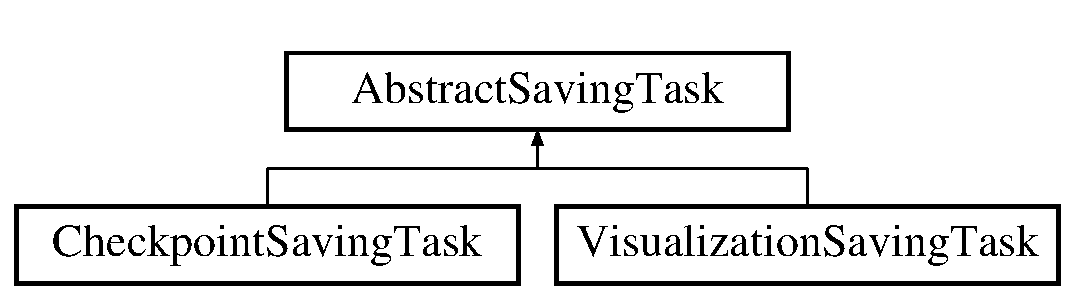
\includegraphics[height=2.000000cm]{d4/da2/class_abstract_saving_task}
\end{center}
\end{figure}
\subsection*{Public Member Functions}
\begin{DoxyCompactItemize}
\item 
virtual void {\bfseries execute} (long long int terminals)=0\hypertarget{class_abstract_saving_task_a77f5a339c32da02cfc87f9834cc15aee}{}\label{class_abstract_saving_task_a77f5a339c32da02cfc87f9834cc15aee}

\end{DoxyCompactItemize}


\subsection{Detailed Description}
Abstract class part of an executer design pattern. Each time a tree is saved a set of executers will write the tree content. Different executers provide specific persistance of the tree, such as the generation of C\+CO files or V\+TK, depending if is a checkpoint for further tree generation or just a visualisation temporal file. 

The documentation for this class was generated from the following files\+:\begin{DoxyCompactItemize}
\item 
io/task/Abstract\+Saving\+Task.\+h\item 
io/task/Abstract\+Saving\+Task.\+cpp\end{DoxyCompactItemize}

\hypertarget{class_abstract_stat_manipulator}{}\section{Abstract\+Stat\+Manipulator Class Reference}
\label{class_abstract_stat_manipulator}\index{Abstract\+Stat\+Manipulator@{Abstract\+Stat\+Manipulator}}
Inheritance diagram for Abstract\+Stat\+Manipulator\+:\begin{figure}[H]
\begin{center}
\leavevmode
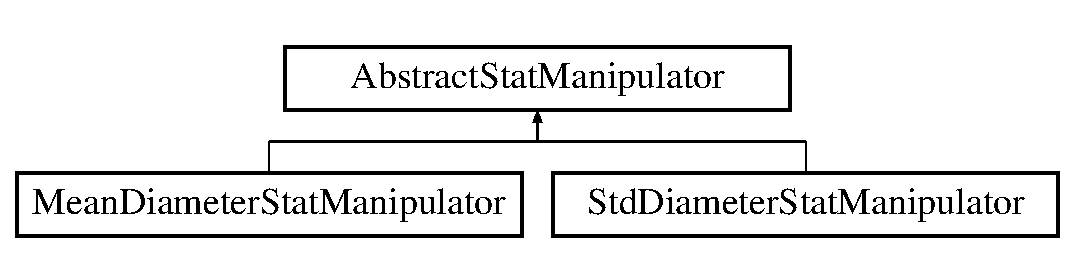
\includegraphics[height=2.000000cm]{class_abstract_stat_manipulator}
\end{center}
\end{figure}
\subsection*{Public Member Functions}
\begin{DoxyCompactItemize}
\item 
\mbox{\Hypertarget{class_abstract_stat_manipulator_aaea26f915b7a0a27c5439438506fd8b6}\label{class_abstract_stat_manipulator_aaea26f915b7a0a27c5439438506fd8b6}} 
virtual double {\bfseries compute} (vector$<$ \mbox{\hyperlink{structvessel}{vessel}} $\ast$$>$ vessels)=0
\end{DoxyCompactItemize}


The documentation for this class was generated from the following files\+:\begin{DoxyCompactItemize}
\item 
stats/Abstract\+Stat\+Manipulator.\+h\item 
stats/Abstract\+Stat\+Manipulator.\+cpp\end{DoxyCompactItemize}

\hypertarget{class_abstract_structured_c_c_o_tree}{}\section{Abstract\+Structured\+C\+C\+O\+Tree Class Reference}
\label{class_abstract_structured_c_c_o_tree}\index{Abstract\+Structured\+C\+C\+O\+Tree@{Abstract\+Structured\+C\+C\+O\+Tree}}


{\ttfamily \#include $<$Abstract\+Structured\+C\+C\+O\+Tree.\+h$>$}

Inheritance diagram for Abstract\+Structured\+C\+C\+O\+Tree\+:\begin{figure}[H]
\begin{center}
\leavevmode
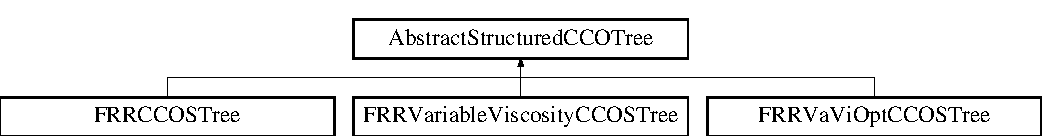
\includegraphics[height=1.821138cm]{df/dae/class_abstract_structured_c_c_o_tree}
\end{center}
\end{figure}
\subsection*{Public Member Functions}
\begin{DoxyCompactItemize}
\item 
\hyperlink{class_abstract_structured_c_c_o_tree_a0a7c83918e4ed64d8e7d371e1c90e4a1}{Abstract\+Structured\+C\+C\+O\+Tree} (\hyperlink{class_generator_data}{Generator\+Data} $\ast$\hyperlink{class_abstract_structured_c_c_o_tree_af1836d7ed2156f3cf9cc311edfdc49b1}{instance\+Data})
\item 
\hyperlink{class_abstract_structured_c_c_o_tree_aafb34c1fbc00f683908dc933ae333599}{Abstract\+Structured\+C\+C\+O\+Tree} (\hyperlink{structpoint}{point} xi, double qi, \hyperlink{class_abstract_constraint_function}{Abstract\+Constraint\+Function}$<$ double, int $>$ $\ast$gam, \hyperlink{class_abstract_constraint_function}{Abstract\+Constraint\+Function}$<$ double, int $>$ $\ast$eps\+Lim, \hyperlink{class_abstract_constraint_function}{Abstract\+Constraint\+Function}$<$ double, int $>$ $\ast$nu, double min\+Angle, double ref\+Pressure, \hyperlink{class_generator_data}{Generator\+Data} $\ast$\hyperlink{class_abstract_structured_c_c_o_tree_af1836d7ed2156f3cf9cc311edfdc49b1}{instance\+Data})
\item 
virtual \hyperlink{class_abstract_structured_c_c_o_tree_a0b1829c729e83d1e577ad8724e5298a7}{$\sim$\+Abstract\+Structured\+C\+C\+O\+Tree} ()
\item 
virtual void \hyperlink{class_abstract_structured_c_c_o_tree_a09cb70d5e23065273d87dd0c0434e1c5}{get\+Closest\+Tree\+Point} (\hyperlink{structpoint}{point} x\+New, \hyperlink{structpoint}{point} $\ast$x\+Bif, double $\ast$dist)=0
\item 
virtual vector$<$ \hyperlink{structvessel}{vessel} $\ast$ $>$ \hyperlink{class_abstract_structured_c_c_o_tree_a0371a4c9a5e8ddfd8b0cc8d811d60f04}{get\+Close\+Segments} (\hyperlink{structpoint}{point} x\+New, \hyperlink{class_abstract_domain}{Abstract\+Domain} $\ast$domain, int $\ast$n\+Found)=0
\item 
virtual void \hyperlink{class_abstract_structured_c_c_o_tree_af592741d1d89d62834e9d58a72cb40af}{add\+Vessel} (\hyperlink{structpoint}{point} x\+Prox, \hyperlink{structpoint}{point} x\+Dist, \hyperlink{structvessel}{vessel} $\ast$parent)=0
\item 
virtual int \hyperlink{class_abstract_structured_c_c_o_tree_ac566ae7f8357ce1f61f624d87a9daf86}{test\+Vessel} (\hyperlink{structpoint}{point} x\+New, \hyperlink{structvessel}{vessel} $\ast$parent, \hyperlink{class_abstract_domain}{Abstract\+Domain} $\ast$domain, vector$<$ \hyperlink{structvessel}{vessel} $\ast$ $>$ neighbors, double dlim, \hyperlink{structpoint}{point} $\ast$x\+Bif, double $\ast$cost)=0
\item 
void \hyperlink{class_abstract_structured_c_c_o_tree_ad9a13faaabbb462ded459e5a9591b1b4}{compute\+Pressure} (\hyperlink{structvessel}{vessel} $\ast$root)
\item 
virtual void \hyperlink{class_abstract_structured_c_c_o_tree_ab28e036b4d82004ab4bafa964d7f7c97}{print} ()=0
\item 
void \hyperlink{class_abstract_structured_c_c_o_tree_a4886ea6cee8ac3771a30727825ab1092}{store\+V\+TK} (string filename)
\item 
void \hyperlink{class_abstract_structured_c_c_o_tree_a0f1333161fd43de84314b827ac82f5f5}{store\+V\+TK} (string filename, unsigned int mode)
\item 
virtual void \hyperlink{class_abstract_structured_c_c_o_tree_ae948aa5785cca23860f98acd91315480}{save} (string filename)
\item 
virtual string \hyperlink{class_abstract_structured_c_c_o_tree_a32e56a263498bc04c3c552fc7de30554}{get\+Tree\+Name} ()=0
\item 
vector$<$ vector$<$ double $>$ $>$ \hyperlink{class_abstract_structured_c_c_o_tree_a9de1840215390c5a396809b430347cbd}{get\+Vertices} ()
\item 
vector$<$ vector$<$ int $>$ $>$ \hyperlink{class_abstract_structured_c_c_o_tree_a9b3f4467c0955b99278495050932b6e0}{get\+Connectivity} ()
\item 
void \hyperlink{class_abstract_structured_c_c_o_tree_a6be7092ab1cce8991b1b43fb527675cb}{print\+Vtk\+Tree} ()
\item 
long long int \hyperlink{class_abstract_structured_c_c_o_tree_a0ddb28f7cb449f1c529f8b1f80af2756}{get\+N\+Terminals} ()
\item 
\hyperlink{structpoint}{point} \hyperlink{class_abstract_structured_c_c_o_tree_a51900d064692213a11fab39ea1d880ef}{get\+X\+Prox} ()
\item 
double \hyperlink{class_abstract_structured_c_c_o_tree_a5235386424ce702fceca86bf2521dd7c}{get\+Q\+Prox} ()
\item 
\hyperlink{class_abstract_constraint_function}{Abstract\+Constraint\+Function}$<$ double, int $>$ $\ast$ \hyperlink{class_abstract_structured_c_c_o_tree_ad5e5bce5de7fb13c313d8031c214cf8f}{get\+Eps\+Lim} ()
\item 
\hyperlink{class_abstract_constraint_function}{Abstract\+Constraint\+Function}$<$ double, int $>$ $\ast$ \hyperlink{class_abstract_structured_c_c_o_tree_a57459e2a67c1254ecdf9f065e83e8c14}{get\+Gam} ()
\item 
\hyperlink{class_abstract_constraint_function}{Abstract\+Constraint\+Function}$<$ double, int $>$ $\ast$ \hyperlink{class_abstract_structured_c_c_o_tree_ad215df279dbc1eaf0f5128836c287819}{get\+Nu} ()
\item 
\hyperlink{structvessel}{vessel} $\ast$ \hyperlink{class_abstract_structured_c_c_o_tree_a8db5e5d1d1e0ebfc8c0a464ab59f916f}{get\+Root} ()
\item 
vtk\+Smart\+Pointer$<$ vtk\+Poly\+Data $>$ \hyperlink{class_abstract_structured_c_c_o_tree_a39f4b8a140cafb99d4fbf65b7d042d88}{get\+Vtk\+Tree} ()
\item 
const vector$<$ \hyperlink{structvessel}{vessel} $\ast$ $>$ \& \hyperlink{class_abstract_structured_c_c_o_tree_af06ce1d020f29716c42a57ea6c103ef1}{get\+Segments} () const 
\item 
double \hyperlink{class_abstract_structured_c_c_o_tree_a35151df888863067191f01d7aa88f0fd}{get\+Dp} () const 
\item 
double \hyperlink{class_abstract_structured_c_c_o_tree_aa4c2e32280c2df85be165b5f53175b9c}{get\+Min\+Angle} () const 
\item 
\hyperlink{class_generator_data}{Generator\+Data} $\ast$ \hyperlink{class_abstract_structured_c_c_o_tree_a343ffe5c45fe18d60b5fd78530dc24f4}{get\+Instance\+Data} ()
\item 
long long int \hyperlink{class_abstract_structured_c_c_o_tree_a7e46f512fe32e55e58d6a1c06dd8bccc}{get\+Point\+Counter} () const 
\item 
void \hyperlink{class_abstract_structured_c_c_o_tree_a1b92fc42f2efdc459d96b12776f54b8f}{set\+Eps\+Lim} (\hyperlink{class_abstract_constraint_function}{Abstract\+Constraint\+Function}$<$ double, int $>$ $\ast$eps\+Lim)
\item 
void \hyperlink{class_abstract_structured_c_c_o_tree_a479ac782dcb0132a178013ef7b113bbf}{set\+Gam} (\hyperlink{class_abstract_constraint_function}{Abstract\+Constraint\+Function}$<$ double, int $>$ $\ast$gam)
\item 
void \hyperlink{class_abstract_structured_c_c_o_tree_ad48f5dd124e15a246d21495e78f96412}{set\+Min\+Angle} (double min\+Angle)
\item 
void \hyperlink{class_abstract_structured_c_c_o_tree_a01f0e3090e61c48d760c25688228a5b2}{set\+Nu} (\hyperlink{class_abstract_constraint_function}{Abstract\+Constraint\+Function}$<$ double, int $>$ $\ast$nu)
\item 
void \hyperlink{class_abstract_structured_c_c_o_tree_a49368c8d7c34f941694cd5cd42a79922}{set\+Point\+Counter} (long long int point\+Counter)
\item 
void \hyperlink{class_abstract_structured_c_c_o_tree_ad19ef66f66f9fdfedfb3ecd47f32c9bd}{set\+Instance\+Data} (\hyperlink{class_generator_data}{Generator\+Data} $\ast$\hyperlink{class_abstract_structured_c_c_o_tree_af1836d7ed2156f3cf9cc311edfdc49b1}{instance\+Data})
\end{DoxyCompactItemize}
\subsection*{Protected Member Functions}
\begin{DoxyCompactItemize}
\item 
void \hyperlink{class_abstract_structured_c_c_o_tree_a02c0800be71a2da7ea0134cf9ced320a}{save\+Vessel} (\hyperlink{structvessel}{vessel} $\ast$current\+Vessel, ofstream $\ast$out\+File)
\item 
virtual void \hyperlink{class_abstract_structured_c_c_o_tree_a16fb849f7fa74189c6b74c60ce59e776}{save\+Tree} (ofstream $\ast$out\+File)
\item 
vector$<$ \hyperlink{structvessel}{vessel} $\ast$ $>$ \hyperlink{class_abstract_structured_c_c_o_tree_a1e8da693a2c1b559c83e77198dfb0305}{create\+V\+T\+K\+Index} ()
\item 
void \hyperlink{class_abstract_structured_c_c_o_tree_a167b0a813fb29104fd63c374e6180f0f}{generate\+V\+T\+Kstructures} (\hyperlink{structvessel}{vessel} $\ast$root)
\item 
void \hyperlink{class_abstract_structured_c_c_o_tree_ad79bddcfc045a3d558669f628ee323f5}{update\+Segment\+Vtk\+Lines} ()
\item 
long long int \hyperlink{class_abstract_structured_c_c_o_tree_a541110b1a550a8a521306caa25d11e45}{count\+Terminals} (\hyperlink{structvessel}{vessel} $\ast$root)
\item 
double \hyperlink{class_abstract_structured_c_c_o_tree_abfb3473aada3b001ec83c3f0ab3e7e03}{compute\+Tree\+Cost} (\hyperlink{structvessel}{vessel} $\ast$root, double parent\+Radius)
\end{DoxyCompactItemize}
\subsection*{Protected Attributes}
\begin{DoxyCompactItemize}
\item 
\hyperlink{class_generator_data}{Generator\+Data} $\ast$ \hyperlink{class_abstract_structured_c_c_o_tree_af1836d7ed2156f3cf9cc311edfdc49b1}{instance\+Data}
\item 
\hyperlink{structpoint}{point} {\bfseries x\+Perf}\hypertarget{class_abstract_structured_c_c_o_tree_a91bae86bcc7ea48856d8c2e4e7edb86b}{}\label{class_abstract_structured_c_c_o_tree_a91bae86bcc7ea48856d8c2e4e7edb86b}

\item 
double {\bfseries q\+Prox}\hypertarget{class_abstract_structured_c_c_o_tree_a11a4dfefc0d9e597f88c5a5fb90bde13}{}\label{class_abstract_structured_c_c_o_tree_a11a4dfefc0d9e597f88c5a5fb90bde13}

\item 
\hyperlink{class_abstract_constraint_function}{Abstract\+Constraint\+Function}$<$ double, int $>$ $\ast$ {\bfseries gam}\hypertarget{class_abstract_structured_c_c_o_tree_aade49db0f344bd2872f41455244667fa}{}\label{class_abstract_structured_c_c_o_tree_aade49db0f344bd2872f41455244667fa}

\item 
\hyperlink{class_abstract_constraint_function}{Abstract\+Constraint\+Function}$<$ double, int $>$ $\ast$ {\bfseries eps\+Lim}\hypertarget{class_abstract_structured_c_c_o_tree_a70cbbe2044e34b9ca4f77369bdfbf8c7}{}\label{class_abstract_structured_c_c_o_tree_a70cbbe2044e34b9ca4f77369bdfbf8c7}

\item 
\hyperlink{class_abstract_constraint_function}{Abstract\+Constraint\+Function}$<$ double, int $>$ $\ast$ {\bfseries nu}\hypertarget{class_abstract_structured_c_c_o_tree_a48e190d08356cb9a6d830d5231a8af40}{}\label{class_abstract_structured_c_c_o_tree_a48e190d08356cb9a6d830d5231a8af40}

\item 
double {\bfseries min\+Angle}\hypertarget{class_abstract_structured_c_c_o_tree_a73011b8853496a96d1be0578c5a21767}{}\label{class_abstract_structured_c_c_o_tree_a73011b8853496a96d1be0578c5a21767}

\item 
double {\bfseries ref\+Pressure}\hypertarget{class_abstract_structured_c_c_o_tree_a9caff71edb514f848fde54254c3a79dc}{}\label{class_abstract_structured_c_c_o_tree_a9caff71edb514f848fde54254c3a79dc}

\item 
\hyperlink{structvessel}{vessel} $\ast$ {\bfseries root}\hypertarget{class_abstract_structured_c_c_o_tree_acb2dfd906f3df9e57cdff7afcaa22073}{}\label{class_abstract_structured_c_c_o_tree_acb2dfd906f3df9e57cdff7afcaa22073}

\item 
double {\bfseries psi\+Factor}\hypertarget{class_abstract_structured_c_c_o_tree_a4cb13a700e00678a3fe08700294d68df}{}\label{class_abstract_structured_c_c_o_tree_a4cb13a700e00678a3fe08700294d68df}

\item 
double {\bfseries dp}\hypertarget{class_abstract_structured_c_c_o_tree_a9420e7bcfe82070a1c5776bdd3116d55}{}\label{class_abstract_structured_c_c_o_tree_a9420e7bcfe82070a1c5776bdd3116d55}

\item 
long long {\bfseries n\+Terms}\hypertarget{class_abstract_structured_c_c_o_tree_ab3069695ccaeffad30b4c2d495c55be6}{}\label{class_abstract_structured_c_c_o_tree_ab3069695ccaeffad30b4c2d495c55be6}

\item 
vtk\+Smart\+Pointer$<$ vtk\+Poly\+Data $>$ {\bfseries vtk\+Tree}\hypertarget{class_abstract_structured_c_c_o_tree_a9de62ed39b142c10f9bb781d31632763}{}\label{class_abstract_structured_c_c_o_tree_a9de62ed39b142c10f9bb781d31632763}

\item 
vtk\+Smart\+Pointer$<$ vtk\+Cell\+Locator $>$ {\bfseries vtk\+Tree\+Locator}\hypertarget{class_abstract_structured_c_c_o_tree_a0c25112aff221d43baea3a7e849c6a76}{}\label{class_abstract_structured_c_c_o_tree_a0c25112aff221d43baea3a7e849c6a76}

\item 
vector$<$ \hyperlink{structvessel}{vessel} $\ast$ $>$ {\bfseries segments}\hypertarget{class_abstract_structured_c_c_o_tree_a260ff9f6dfab06e63574655f95ed4ee3}{}\label{class_abstract_structured_c_c_o_tree_a260ff9f6dfab06e63574655f95ed4ee3}

\item 
long long int {\bfseries point\+Counter}\hypertarget{class_abstract_structured_c_c_o_tree_a715e34fae28f228a82a7dffdcf14c4b7}{}\label{class_abstract_structured_c_c_o_tree_a715e34fae28f228a82a7dffdcf14c4b7}

\end{DoxyCompactItemize}


\subsection{Detailed Description}
Generic C\+CO Tree structure and required methods. 

\subsection{Constructor \& Destructor Documentation}
\index{Abstract\+Structured\+C\+C\+O\+Tree@{Abstract\+Structured\+C\+C\+O\+Tree}!Abstract\+Structured\+C\+C\+O\+Tree@{Abstract\+Structured\+C\+C\+O\+Tree}}
\index{Abstract\+Structured\+C\+C\+O\+Tree@{Abstract\+Structured\+C\+C\+O\+Tree}!Abstract\+Structured\+C\+C\+O\+Tree@{Abstract\+Structured\+C\+C\+O\+Tree}}
\subsubsection[{\texorpdfstring{Abstract\+Structured\+C\+C\+O\+Tree(\+Generator\+Data $\ast$instance\+Data)}{AbstractStructuredCCOTree(GeneratorData *instanceData)}}]{\setlength{\rightskip}{0pt plus 5cm}Abstract\+Structured\+C\+C\+O\+Tree\+::\+Abstract\+Structured\+C\+C\+O\+Tree (
\begin{DoxyParamCaption}
\item[{{\bf Generator\+Data} $\ast$}]{instance\+Data}
\end{DoxyParamCaption}
)}\hypertarget{class_abstract_structured_c_c_o_tree_a0a7c83918e4ed64d8e7d371e1c90e4a1}{}\label{class_abstract_structured_c_c_o_tree_a0a7c83918e4ed64d8e7d371e1c90e4a1}
Constructor for tree with no parameters, convenient to create a tree and load its parameters later. 
\begin{DoxyParams}{Parameters}
{\em instance\+Data} & Global parameters for instance behavior (amount of tries per bifurcation, point tries before d\+Lim reduction, etc.). \\
\hline
\end{DoxyParams}
\index{Abstract\+Structured\+C\+C\+O\+Tree@{Abstract\+Structured\+C\+C\+O\+Tree}!Abstract\+Structured\+C\+C\+O\+Tree@{Abstract\+Structured\+C\+C\+O\+Tree}}
\index{Abstract\+Structured\+C\+C\+O\+Tree@{Abstract\+Structured\+C\+C\+O\+Tree}!Abstract\+Structured\+C\+C\+O\+Tree@{Abstract\+Structured\+C\+C\+O\+Tree}}
\subsubsection[{\texorpdfstring{Abstract\+Structured\+C\+C\+O\+Tree(point xi, double qi, Abstract\+Constraint\+Function$<$ double, int $>$ $\ast$gam, Abstract\+Constraint\+Function$<$ double, int $>$ $\ast$eps\+Lim, Abstract\+Constraint\+Function$<$ double, int $>$ $\ast$nu, double min\+Angle, double ref\+Pressure, Generator\+Data $\ast$instance\+Data)}{AbstractStructuredCCOTree(point xi, double qi, AbstractConstraintFunction< double, int > *gam, AbstractConstraintFunction< double, int > *epsLim, AbstractConstraintFunction< double, int > *nu, double minAngle, double refPressure, GeneratorData *instanceData)}}]{\setlength{\rightskip}{0pt plus 5cm}Abstract\+Structured\+C\+C\+O\+Tree\+::\+Abstract\+Structured\+C\+C\+O\+Tree (
\begin{DoxyParamCaption}
\item[{{\bf point}}]{xi, }
\item[{double}]{qi, }
\item[{{\bf Abstract\+Constraint\+Function}$<$ double, int $>$ $\ast$}]{gam, }
\item[{{\bf Abstract\+Constraint\+Function}$<$ double, int $>$ $\ast$}]{eps\+Lim, }
\item[{{\bf Abstract\+Constraint\+Function}$<$ double, int $>$ $\ast$}]{nu, }
\item[{double}]{min\+Angle, }
\item[{double}]{ref\+Pressure, }
\item[{{\bf Generator\+Data} $\ast$}]{instance\+Data}
\end{DoxyParamCaption}
)}\hypertarget{class_abstract_structured_c_c_o_tree_aafb34c1fbc00f683908dc933ae333599}{}\label{class_abstract_structured_c_c_o_tree_aafb34c1fbc00f683908dc933ae333599}
Common constructor with all parameters necessary for tree generation. 
\begin{DoxyParams}{Parameters}
{\em xi} & Root entry point. \\
\hline
{\em qi} & Flow at {\ttfamily xi}. \\
\hline
{\em gam} & Function for the exponential coefficient of the Murray Law depending on the bifurcation level. \\
\hline
{\em eps\+Lim} & Function of the symmetry ratio (ratio between the radius of the smallest over the biggest sibling) depending on the bifurcation level. \\
\hline
{\em nu} & Blood viscosity depending on the bifurcation level. \\
\hline
{\em min\+Angle} & Lowest angle allowed at the new bifurcation. \\
\hline
{\em ref\+Pressure} & Distal reference pressure for the tree. \\
\hline
{\em instance\+Data} & Parameters for this stage generation. \\
\hline
\end{DoxyParams}
\index{Abstract\+Structured\+C\+C\+O\+Tree@{Abstract\+Structured\+C\+C\+O\+Tree}!````~Abstract\+Structured\+C\+C\+O\+Tree@{$\sim$\+Abstract\+Structured\+C\+C\+O\+Tree}}
\index{````~Abstract\+Structured\+C\+C\+O\+Tree@{$\sim$\+Abstract\+Structured\+C\+C\+O\+Tree}!Abstract\+Structured\+C\+C\+O\+Tree@{Abstract\+Structured\+C\+C\+O\+Tree}}
\subsubsection[{\texorpdfstring{$\sim$\+Abstract\+Structured\+C\+C\+O\+Tree()}{~AbstractStructuredCCOTree()}}]{\setlength{\rightskip}{0pt plus 5cm}Abstract\+Structured\+C\+C\+O\+Tree\+::$\sim$\+Abstract\+Structured\+C\+C\+O\+Tree (
\begin{DoxyParamCaption}
{}
\end{DoxyParamCaption}
)\hspace{0.3cm}{\ttfamily [virtual]}}\hypertarget{class_abstract_structured_c_c_o_tree_a0b1829c729e83d1e577ad8724e5298a7}{}\label{class_abstract_structured_c_c_o_tree_a0b1829c729e83d1e577ad8724e5298a7}
Common destructor. 

\subsection{Member Function Documentation}
\index{Abstract\+Structured\+C\+C\+O\+Tree@{Abstract\+Structured\+C\+C\+O\+Tree}!add\+Vessel@{add\+Vessel}}
\index{add\+Vessel@{add\+Vessel}!Abstract\+Structured\+C\+C\+O\+Tree@{Abstract\+Structured\+C\+C\+O\+Tree}}
\subsubsection[{\texorpdfstring{add\+Vessel(point x\+Prox, point x\+Dist, vessel $\ast$parent)=0}{addVessel(point xProx, point xDist, vessel *parent)=0}}]{\setlength{\rightskip}{0pt plus 5cm}virtual void Abstract\+Structured\+C\+C\+O\+Tree\+::add\+Vessel (
\begin{DoxyParamCaption}
\item[{{\bf point}}]{x\+Prox, }
\item[{{\bf point}}]{x\+Dist, }
\item[{{\bf vessel} $\ast$}]{parent}
\end{DoxyParamCaption}
)\hspace{0.3cm}{\ttfamily [pure virtual]}}\hypertarget{class_abstract_structured_c_c_o_tree_af592741d1d89d62834e9d58a72cb40af}{}\label{class_abstract_structured_c_c_o_tree_af592741d1d89d62834e9d58a72cb40af}
Adds a new vessel to the C\+CO tree. 
\begin{DoxyParams}{Parameters}
{\em x\+Prox} & and \\
\hline
{\em x\+Dist} & are the proximal and distal nodes of the new vessel and \\
\hline
{\em parent} & is the attachment parent vessel. \\
\hline
{\em x\+Prox} & Proximal point of the new vessel. \\
\hline
{\em x\+Dist} & Distal point of the new vessel. \\
\hline
{\em parent} & Parent to the new vessel. \\
\hline
\end{DoxyParams}


Implemented in \hyperlink{class_f_r_r_va_vi_opt_c_c_o_s_tree_a95c4523a6c2ed20c16d83b62ec6b5873}{F\+R\+R\+Va\+Vi\+Opt\+C\+C\+O\+S\+Tree}, \hyperlink{class_f_r_r_variable_viscosity_c_c_o_s_tree_a494a10a964337b83827012bfc03af194}{F\+R\+R\+Variable\+Viscosity\+C\+C\+O\+S\+Tree}, and \hyperlink{class_f_r_r_c_c_o_s_tree_a91c2d539ccbd91c0f07a4366206e01da}{F\+R\+R\+C\+C\+O\+S\+Tree}.

\index{Abstract\+Structured\+C\+C\+O\+Tree@{Abstract\+Structured\+C\+C\+O\+Tree}!compute\+Pressure@{compute\+Pressure}}
\index{compute\+Pressure@{compute\+Pressure}!Abstract\+Structured\+C\+C\+O\+Tree@{Abstract\+Structured\+C\+C\+O\+Tree}}
\subsubsection[{\texorpdfstring{compute\+Pressure(vessel $\ast$root)}{computePressure(vessel *root)}}]{\setlength{\rightskip}{0pt plus 5cm}void Abstract\+Structured\+C\+C\+O\+Tree\+::compute\+Pressure (
\begin{DoxyParamCaption}
\item[{{\bf vessel} $\ast$}]{root}
\end{DoxyParamCaption}
)}\hypertarget{class_abstract_structured_c_c_o_tree_ad9a13faaabbb462ded459e5a9591b1b4}{}\label{class_abstract_structured_c_c_o_tree_ad9a13faaabbb462ded459e5a9591b1b4}
Computes the pressure for the whole tree for a given reference pressure P\+\_\+r (default P\+\_\+r=0 Pa). 
\begin{DoxyParams}{Parameters}
{\em root} & Tree root. \\
\hline
\end{DoxyParams}
\index{Abstract\+Structured\+C\+C\+O\+Tree@{Abstract\+Structured\+C\+C\+O\+Tree}!compute\+Tree\+Cost@{compute\+Tree\+Cost}}
\index{compute\+Tree\+Cost@{compute\+Tree\+Cost}!Abstract\+Structured\+C\+C\+O\+Tree@{Abstract\+Structured\+C\+C\+O\+Tree}}
\subsubsection[{\texorpdfstring{compute\+Tree\+Cost(vessel $\ast$root, double parent\+Radius)}{computeTreeCost(vessel *root, double parentRadius)}}]{\setlength{\rightskip}{0pt plus 5cm}double Abstract\+Structured\+C\+C\+O\+Tree\+::compute\+Tree\+Cost (
\begin{DoxyParamCaption}
\item[{{\bf vessel} $\ast$}]{root, }
\item[{double}]{parent\+Radius}
\end{DoxyParamCaption}
)\hspace{0.3cm}{\ttfamily [protected]}}\hypertarget{class_abstract_structured_c_c_o_tree_abfb3473aada3b001ec83c3f0ab3e7e03}{}\label{class_abstract_structured_c_c_o_tree_abfb3473aada3b001ec83c3f0ab3e7e03}
Computes the total tree volume, if the geometric constraint is not satisfied, it returns I\+N\+F\+I\+N\+I\+TY. 
\begin{DoxyParams}{Parameters}
{\em root} & \\
\hline
{\em parent\+Radius} & \\
\hline
\end{DoxyParams}
\begin{DoxyReturn}{Returns}
Total tree volume. 
\end{DoxyReturn}
\index{Abstract\+Structured\+C\+C\+O\+Tree@{Abstract\+Structured\+C\+C\+O\+Tree}!count\+Terminals@{count\+Terminals}}
\index{count\+Terminals@{count\+Terminals}!Abstract\+Structured\+C\+C\+O\+Tree@{Abstract\+Structured\+C\+C\+O\+Tree}}
\subsubsection[{\texorpdfstring{count\+Terminals(vessel $\ast$root)}{countTerminals(vessel *root)}}]{\setlength{\rightskip}{0pt plus 5cm}long long int Abstract\+Structured\+C\+C\+O\+Tree\+::count\+Terminals (
\begin{DoxyParamCaption}
\item[{{\bf vessel} $\ast$}]{root}
\end{DoxyParamCaption}
)\hspace{0.3cm}{\ttfamily [protected]}}\hypertarget{class_abstract_structured_c_c_o_tree_a541110b1a550a8a521306caa25d11e45}{}\label{class_abstract_structured_c_c_o_tree_a541110b1a550a8a521306caa25d11e45}
Counts recursively all terminals of the subtree with {\ttfamily root} as root. 
\begin{DoxyParams}{Parameters}
{\em root} & Root of the subtree. \\
\hline
\end{DoxyParams}
\begin{DoxyReturn}{Returns}
Amount of terminals in the subtree. 
\end{DoxyReturn}
\index{Abstract\+Structured\+C\+C\+O\+Tree@{Abstract\+Structured\+C\+C\+O\+Tree}!create\+V\+T\+K\+Index@{create\+V\+T\+K\+Index}}
\index{create\+V\+T\+K\+Index@{create\+V\+T\+K\+Index}!Abstract\+Structured\+C\+C\+O\+Tree@{Abstract\+Structured\+C\+C\+O\+Tree}}
\subsubsection[{\texorpdfstring{create\+V\+T\+K\+Index()}{createVTKIndex()}}]{\setlength{\rightskip}{0pt plus 5cm}vector$<$ {\bf vessel} $\ast$ $>$ Abstract\+Structured\+C\+C\+O\+Tree\+::create\+V\+T\+K\+Index (
\begin{DoxyParamCaption}
{}
\end{DoxyParamCaption}
)\hspace{0.3cm}{\ttfamily [protected]}}\hypertarget{class_abstract_structured_c_c_o_tree_a1e8da693a2c1b559c83e77198dfb0305}{}\label{class_abstract_structured_c_c_o_tree_a1e8da693a2c1b559c83e77198dfb0305}
Creates an ordered vector with all V\+TK identifiers of the vessels in the current tree. \begin{DoxyReturn}{Returns}
Vector with all V\+TK identifiers of the vessels in the current tree. 
\end{DoxyReturn}
\index{Abstract\+Structured\+C\+C\+O\+Tree@{Abstract\+Structured\+C\+C\+O\+Tree}!generate\+V\+T\+Kstructures@{generate\+V\+T\+Kstructures}}
\index{generate\+V\+T\+Kstructures@{generate\+V\+T\+Kstructures}!Abstract\+Structured\+C\+C\+O\+Tree@{Abstract\+Structured\+C\+C\+O\+Tree}}
\subsubsection[{\texorpdfstring{generate\+V\+T\+Kstructures(vessel $\ast$root)}{generateVTKstructures(vessel *root)}}]{\setlength{\rightskip}{0pt plus 5cm}void Abstract\+Structured\+C\+C\+O\+Tree\+::generate\+V\+T\+Kstructures (
\begin{DoxyParamCaption}
\item[{{\bf vessel} $\ast$}]{root}
\end{DoxyParamCaption}
)\hspace{0.3cm}{\ttfamily [protected]}}\hypertarget{class_abstract_structured_c_c_o_tree_a167b0a813fb29104fd63c374e6180f0f}{}\label{class_abstract_structured_c_c_o_tree_a167b0a813fb29104fd63c374e6180f0f}
Generates all V\+TK objects of the vessels loaded in the current tree. 
\begin{DoxyParams}{Parameters}
{\em root} & Root of the tree. \\
\hline
\end{DoxyParams}
\index{Abstract\+Structured\+C\+C\+O\+Tree@{Abstract\+Structured\+C\+C\+O\+Tree}!get\+Close\+Segments@{get\+Close\+Segments}}
\index{get\+Close\+Segments@{get\+Close\+Segments}!Abstract\+Structured\+C\+C\+O\+Tree@{Abstract\+Structured\+C\+C\+O\+Tree}}
\subsubsection[{\texorpdfstring{get\+Close\+Segments(point x\+New, Abstract\+Domain $\ast$domain, int $\ast$n\+Found)=0}{getCloseSegments(point xNew, AbstractDomain *domain, int *nFound)=0}}]{\setlength{\rightskip}{0pt plus 5cm}virtual vector$<${\bf vessel} $\ast$$>$ Abstract\+Structured\+C\+C\+O\+Tree\+::get\+Close\+Segments (
\begin{DoxyParamCaption}
\item[{{\bf point}}]{x\+New, }
\item[{{\bf Abstract\+Domain} $\ast$}]{domain, }
\item[{int $\ast$}]{n\+Found}
\end{DoxyParamCaption}
)\hspace{0.3cm}{\ttfamily [pure virtual]}}\hypertarget{class_abstract_structured_c_c_o_tree_a0371a4c9a5e8ddfd8b0cc8d811d60f04}{}\label{class_abstract_structured_c_c_o_tree_a0371a4c9a5e8ddfd8b0cc8d811d60f04}
Return the segments in a close neighborhood of {\ttfamily x\+New}. The neighborhood is computed based on the perfusion volume indicated by {\ttfamily domain}. 
\begin{DoxyParams}{Parameters}
{\em x\+New} & Center point of the neighborhood of interest. \\
\hline
{\em domain} & Domain of the segments. \\
\hline
{\em n\+Found} & Amount of segments in the neighborhood. \\
\hline
\end{DoxyParams}
\begin{DoxyReturn}{Returns}
Array of segments in the neighborhood of {\ttfamily x\+New}. 
\end{DoxyReturn}


Implemented in \hyperlink{class_f_r_r_va_vi_opt_c_c_o_s_tree_a88826c9f37705bcce03374d920eff19a}{F\+R\+R\+Va\+Vi\+Opt\+C\+C\+O\+S\+Tree}, \hyperlink{class_f_r_r_variable_viscosity_c_c_o_s_tree_a41e4e3406e5f78d50d5e597bad4950cd}{F\+R\+R\+Variable\+Viscosity\+C\+C\+O\+S\+Tree}, and \hyperlink{class_f_r_r_c_c_o_s_tree_a51eeb636beadda63f0496ca3385c60f1}{F\+R\+R\+C\+C\+O\+S\+Tree}.

\index{Abstract\+Structured\+C\+C\+O\+Tree@{Abstract\+Structured\+C\+C\+O\+Tree}!get\+Closest\+Tree\+Point@{get\+Closest\+Tree\+Point}}
\index{get\+Closest\+Tree\+Point@{get\+Closest\+Tree\+Point}!Abstract\+Structured\+C\+C\+O\+Tree@{Abstract\+Structured\+C\+C\+O\+Tree}}
\subsubsection[{\texorpdfstring{get\+Closest\+Tree\+Point(point x\+New, point $\ast$x\+Bif, double $\ast$dist)=0}{getClosestTreePoint(point xNew, point *xBif, double *dist)=0}}]{\setlength{\rightskip}{0pt plus 5cm}virtual void Abstract\+Structured\+C\+C\+O\+Tree\+::get\+Closest\+Tree\+Point (
\begin{DoxyParamCaption}
\item[{{\bf point}}]{x\+New, }
\item[{{\bf point} $\ast$}]{x\+Bif, }
\item[{double $\ast$}]{dist}
\end{DoxyParamCaption}
)\hspace{0.3cm}{\ttfamily [pure virtual]}}\hypertarget{class_abstract_structured_c_c_o_tree_a09cb70d5e23065273d87dd0c0434e1c5}{}\label{class_abstract_structured_c_c_o_tree_a09cb70d5e23065273d87dd0c0434e1c5}
Returns the closest point in the C\+C\+O\+Tree with respect to {\ttfamily x\+New} point. 
\begin{DoxyParams}{Parameters}
{\em x\+New} & Point from which the minimum distance is computed. \\
\hline
{\em x\+Bif} & Closest point in the tree to {\ttfamily x\+New}. \\
\hline
{\em dist} & Minimum distance between {\ttfamily x\+New} and the tree. \\
\hline
\end{DoxyParams}


Implemented in \hyperlink{class_f_r_r_va_vi_opt_c_c_o_s_tree_a8360ecbbf60ee0e52d4a83f40a3f0154}{F\+R\+R\+Va\+Vi\+Opt\+C\+C\+O\+S\+Tree}, \hyperlink{class_f_r_r_variable_viscosity_c_c_o_s_tree_a224c64cbf18976f660a730c5af0b73a0}{F\+R\+R\+Variable\+Viscosity\+C\+C\+O\+S\+Tree}, and \hyperlink{class_f_r_r_c_c_o_s_tree_a9114689c110d03da69c82bf2a833dcae}{F\+R\+R\+C\+C\+O\+S\+Tree}.

\index{Abstract\+Structured\+C\+C\+O\+Tree@{Abstract\+Structured\+C\+C\+O\+Tree}!get\+Connectivity@{get\+Connectivity}}
\index{get\+Connectivity@{get\+Connectivity}!Abstract\+Structured\+C\+C\+O\+Tree@{Abstract\+Structured\+C\+C\+O\+Tree}}
\subsubsection[{\texorpdfstring{get\+Connectivity()}{getConnectivity()}}]{\setlength{\rightskip}{0pt plus 5cm}vector$<$ vector$<$ int $>$ $>$ Abstract\+Structured\+C\+C\+O\+Tree\+::get\+Connectivity (
\begin{DoxyParamCaption}
{}
\end{DoxyParamCaption}
)}\hypertarget{class_abstract_structured_c_c_o_tree_a9b3f4467c0955b99278495050932b6e0}{}\label{class_abstract_structured_c_c_o_tree_a9b3f4467c0955b99278495050932b6e0}
Returns a vector with one entry per line element of the tree. Each entry contains the identifiers of the points that constitutes the element. \begin{DoxyReturn}{Returns}

\end{DoxyReturn}
\index{Abstract\+Structured\+C\+C\+O\+Tree@{Abstract\+Structured\+C\+C\+O\+Tree}!get\+Dp@{get\+Dp}}
\index{get\+Dp@{get\+Dp}!Abstract\+Structured\+C\+C\+O\+Tree@{Abstract\+Structured\+C\+C\+O\+Tree}}
\subsubsection[{\texorpdfstring{get\+Dp() const }{getDp() const }}]{\setlength{\rightskip}{0pt plus 5cm}double Abstract\+Structured\+C\+C\+O\+Tree\+::get\+Dp (
\begin{DoxyParamCaption}
{}
\end{DoxyParamCaption}
) const}\hypertarget{class_abstract_structured_c_c_o_tree_a35151df888863067191f01d7aa88f0fd}{}\label{class_abstract_structured_c_c_o_tree_a35151df888863067191f01d7aa88f0fd}
Getter of {\ttfamily dp}. \begin{DoxyReturn}{Returns}
{\ttfamily dp}. 
\end{DoxyReturn}
\index{Abstract\+Structured\+C\+C\+O\+Tree@{Abstract\+Structured\+C\+C\+O\+Tree}!get\+Eps\+Lim@{get\+Eps\+Lim}}
\index{get\+Eps\+Lim@{get\+Eps\+Lim}!Abstract\+Structured\+C\+C\+O\+Tree@{Abstract\+Structured\+C\+C\+O\+Tree}}
\subsubsection[{\texorpdfstring{get\+Eps\+Lim()}{getEpsLim()}}]{\setlength{\rightskip}{0pt plus 5cm}{\bf Abstract\+Constraint\+Function}$<$ double, int $>$ $\ast$ Abstract\+Structured\+C\+C\+O\+Tree\+::get\+Eps\+Lim (
\begin{DoxyParamCaption}
{}
\end{DoxyParamCaption}
)}\hypertarget{class_abstract_structured_c_c_o_tree_ad5e5bce5de7fb13c313d8031c214cf8f}{}\label{class_abstract_structured_c_c_o_tree_ad5e5bce5de7fb13c313d8031c214cf8f}
Getter of {\ttfamily eps\+Lim}. \begin{DoxyReturn}{Returns}
{\ttfamily eps\+Lim}. 
\end{DoxyReturn}
\index{Abstract\+Structured\+C\+C\+O\+Tree@{Abstract\+Structured\+C\+C\+O\+Tree}!get\+Gam@{get\+Gam}}
\index{get\+Gam@{get\+Gam}!Abstract\+Structured\+C\+C\+O\+Tree@{Abstract\+Structured\+C\+C\+O\+Tree}}
\subsubsection[{\texorpdfstring{get\+Gam()}{getGam()}}]{\setlength{\rightskip}{0pt plus 5cm}{\bf Abstract\+Constraint\+Function}$<$ double, int $>$ $\ast$ Abstract\+Structured\+C\+C\+O\+Tree\+::get\+Gam (
\begin{DoxyParamCaption}
{}
\end{DoxyParamCaption}
)}\hypertarget{class_abstract_structured_c_c_o_tree_a57459e2a67c1254ecdf9f065e83e8c14}{}\label{class_abstract_structured_c_c_o_tree_a57459e2a67c1254ecdf9f065e83e8c14}
Getter of {\ttfamily gam}. \begin{DoxyReturn}{Returns}
{\ttfamily gam}. 
\end{DoxyReturn}
\index{Abstract\+Structured\+C\+C\+O\+Tree@{Abstract\+Structured\+C\+C\+O\+Tree}!get\+Instance\+Data@{get\+Instance\+Data}}
\index{get\+Instance\+Data@{get\+Instance\+Data}!Abstract\+Structured\+C\+C\+O\+Tree@{Abstract\+Structured\+C\+C\+O\+Tree}}
\subsubsection[{\texorpdfstring{get\+Instance\+Data()}{getInstanceData()}}]{\setlength{\rightskip}{0pt plus 5cm}{\bf Generator\+Data} $\ast$ Abstract\+Structured\+C\+C\+O\+Tree\+::get\+Instance\+Data (
\begin{DoxyParamCaption}
{}
\end{DoxyParamCaption}
)}\hypertarget{class_abstract_structured_c_c_o_tree_a343ffe5c45fe18d60b5fd78530dc24f4}{}\label{class_abstract_structured_c_c_o_tree_a343ffe5c45fe18d60b5fd78530dc24f4}
Getter of {\ttfamily instance\+Data}. \begin{DoxyReturn}{Returns}
{\ttfamily instance\+Data}. 
\end{DoxyReturn}
\index{Abstract\+Structured\+C\+C\+O\+Tree@{Abstract\+Structured\+C\+C\+O\+Tree}!get\+Min\+Angle@{get\+Min\+Angle}}
\index{get\+Min\+Angle@{get\+Min\+Angle}!Abstract\+Structured\+C\+C\+O\+Tree@{Abstract\+Structured\+C\+C\+O\+Tree}}
\subsubsection[{\texorpdfstring{get\+Min\+Angle() const }{getMinAngle() const }}]{\setlength{\rightskip}{0pt plus 5cm}double Abstract\+Structured\+C\+C\+O\+Tree\+::get\+Min\+Angle (
\begin{DoxyParamCaption}
{}
\end{DoxyParamCaption}
) const}\hypertarget{class_abstract_structured_c_c_o_tree_aa4c2e32280c2df85be165b5f53175b9c}{}\label{class_abstract_structured_c_c_o_tree_aa4c2e32280c2df85be165b5f53175b9c}
Getter of {\ttfamily min\+Angle}. \begin{DoxyReturn}{Returns}
{\ttfamily min\+Angle}. 
\end{DoxyReturn}
\index{Abstract\+Structured\+C\+C\+O\+Tree@{Abstract\+Structured\+C\+C\+O\+Tree}!get\+N\+Terminals@{get\+N\+Terminals}}
\index{get\+N\+Terminals@{get\+N\+Terminals}!Abstract\+Structured\+C\+C\+O\+Tree@{Abstract\+Structured\+C\+C\+O\+Tree}}
\subsubsection[{\texorpdfstring{get\+N\+Terminals()}{getNTerminals()}}]{\setlength{\rightskip}{0pt plus 5cm}long long int Abstract\+Structured\+C\+C\+O\+Tree\+::get\+N\+Terminals (
\begin{DoxyParamCaption}
{}
\end{DoxyParamCaption}
)}\hypertarget{class_abstract_structured_c_c_o_tree_a0ddb28f7cb449f1c529f8b1f80af2756}{}\label{class_abstract_structured_c_c_o_tree_a0ddb28f7cb449f1c529f8b1f80af2756}
Returns the amount of terminals in the current tree. \begin{DoxyReturn}{Returns}
Amount of tree terminals. 
\end{DoxyReturn}
\index{Abstract\+Structured\+C\+C\+O\+Tree@{Abstract\+Structured\+C\+C\+O\+Tree}!get\+Nu@{get\+Nu}}
\index{get\+Nu@{get\+Nu}!Abstract\+Structured\+C\+C\+O\+Tree@{Abstract\+Structured\+C\+C\+O\+Tree}}
\subsubsection[{\texorpdfstring{get\+Nu()}{getNu()}}]{\setlength{\rightskip}{0pt plus 5cm}{\bf Abstract\+Constraint\+Function}$<$ double, int $>$ $\ast$ Abstract\+Structured\+C\+C\+O\+Tree\+::get\+Nu (
\begin{DoxyParamCaption}
{}
\end{DoxyParamCaption}
)}\hypertarget{class_abstract_structured_c_c_o_tree_ad215df279dbc1eaf0f5128836c287819}{}\label{class_abstract_structured_c_c_o_tree_ad215df279dbc1eaf0f5128836c287819}
Getter of {\ttfamily nu}. \begin{DoxyReturn}{Returns}
{\ttfamily nu}. 
\end{DoxyReturn}
\index{Abstract\+Structured\+C\+C\+O\+Tree@{Abstract\+Structured\+C\+C\+O\+Tree}!get\+Point\+Counter@{get\+Point\+Counter}}
\index{get\+Point\+Counter@{get\+Point\+Counter}!Abstract\+Structured\+C\+C\+O\+Tree@{Abstract\+Structured\+C\+C\+O\+Tree}}
\subsubsection[{\texorpdfstring{get\+Point\+Counter() const }{getPointCounter() const }}]{\setlength{\rightskip}{0pt plus 5cm}long long int Abstract\+Structured\+C\+C\+O\+Tree\+::get\+Point\+Counter (
\begin{DoxyParamCaption}
{}
\end{DoxyParamCaption}
) const}\hypertarget{class_abstract_structured_c_c_o_tree_a7e46f512fe32e55e58d6a1c06dd8bccc}{}\label{class_abstract_structured_c_c_o_tree_a7e46f512fe32e55e58d6a1c06dd8bccc}
Getter of {\ttfamily point\+Counter}. \begin{DoxyReturn}{Returns}
{\ttfamily point\+Counter}. 
\end{DoxyReturn}
\index{Abstract\+Structured\+C\+C\+O\+Tree@{Abstract\+Structured\+C\+C\+O\+Tree}!get\+Q\+Prox@{get\+Q\+Prox}}
\index{get\+Q\+Prox@{get\+Q\+Prox}!Abstract\+Structured\+C\+C\+O\+Tree@{Abstract\+Structured\+C\+C\+O\+Tree}}
\subsubsection[{\texorpdfstring{get\+Q\+Prox()}{getQProx()}}]{\setlength{\rightskip}{0pt plus 5cm}double Abstract\+Structured\+C\+C\+O\+Tree\+::get\+Q\+Prox (
\begin{DoxyParamCaption}
{}
\end{DoxyParamCaption}
)}\hypertarget{class_abstract_structured_c_c_o_tree_a5235386424ce702fceca86bf2521dd7c}{}\label{class_abstract_structured_c_c_o_tree_a5235386424ce702fceca86bf2521dd7c}
Getter of {\ttfamily q\+Prox}. \begin{DoxyReturn}{Returns}
{\ttfamily q\+Prox} 
\end{DoxyReturn}
\index{Abstract\+Structured\+C\+C\+O\+Tree@{Abstract\+Structured\+C\+C\+O\+Tree}!get\+Root@{get\+Root}}
\index{get\+Root@{get\+Root}!Abstract\+Structured\+C\+C\+O\+Tree@{Abstract\+Structured\+C\+C\+O\+Tree}}
\subsubsection[{\texorpdfstring{get\+Root()}{getRoot()}}]{\setlength{\rightskip}{0pt plus 5cm}{\bf vessel} $\ast$ Abstract\+Structured\+C\+C\+O\+Tree\+::get\+Root (
\begin{DoxyParamCaption}
{}
\end{DoxyParamCaption}
)}\hypertarget{class_abstract_structured_c_c_o_tree_a8db5e5d1d1e0ebfc8c0a464ab59f916f}{}\label{class_abstract_structured_c_c_o_tree_a8db5e5d1d1e0ebfc8c0a464ab59f916f}
Getter of {\ttfamily root}. \begin{DoxyReturn}{Returns}
{\ttfamily root}. 
\end{DoxyReturn}
\index{Abstract\+Structured\+C\+C\+O\+Tree@{Abstract\+Structured\+C\+C\+O\+Tree}!get\+Segments@{get\+Segments}}
\index{get\+Segments@{get\+Segments}!Abstract\+Structured\+C\+C\+O\+Tree@{Abstract\+Structured\+C\+C\+O\+Tree}}
\subsubsection[{\texorpdfstring{get\+Segments() const }{getSegments() const }}]{\setlength{\rightskip}{0pt plus 5cm}const vector$<$ {\bf vessel} $\ast$ $>$ \& Abstract\+Structured\+C\+C\+O\+Tree\+::get\+Segments (
\begin{DoxyParamCaption}
{}
\end{DoxyParamCaption}
) const}\hypertarget{class_abstract_structured_c_c_o_tree_af06ce1d020f29716c42a57ea6c103ef1}{}\label{class_abstract_structured_c_c_o_tree_af06ce1d020f29716c42a57ea6c103ef1}
Getter of {\ttfamily segments}. \begin{DoxyReturn}{Returns}
{\ttfamily segments}. 
\end{DoxyReturn}
\index{Abstract\+Structured\+C\+C\+O\+Tree@{Abstract\+Structured\+C\+C\+O\+Tree}!get\+Tree\+Name@{get\+Tree\+Name}}
\index{get\+Tree\+Name@{get\+Tree\+Name}!Abstract\+Structured\+C\+C\+O\+Tree@{Abstract\+Structured\+C\+C\+O\+Tree}}
\subsubsection[{\texorpdfstring{get\+Tree\+Name()=0}{getTreeName()=0}}]{\setlength{\rightskip}{0pt plus 5cm}virtual string Abstract\+Structured\+C\+C\+O\+Tree\+::get\+Tree\+Name (
\begin{DoxyParamCaption}
{}
\end{DoxyParamCaption}
)\hspace{0.3cm}{\ttfamily [pure virtual]}}\hypertarget{class_abstract_structured_c_c_o_tree_a32e56a263498bc04c3c552fc7de30554}{}\label{class_abstract_structured_c_c_o_tree_a32e56a263498bc04c3c552fc7de30554}
Returns the name of the tree class that implements the Abstract\+C\+C\+O\+Tree. \begin{DoxyReturn}{Returns}
Tree class name. 
\end{DoxyReturn}


Implemented in \hyperlink{class_f_r_r_variable_viscosity_c_c_o_s_tree_aac408960939d867d0a2014f4ced90d4d}{F\+R\+R\+Variable\+Viscosity\+C\+C\+O\+S\+Tree}, \hyperlink{class_f_r_r_va_vi_opt_c_c_o_s_tree_a3c7f7ca4242f71697c421298b3ab968b}{F\+R\+R\+Va\+Vi\+Opt\+C\+C\+O\+S\+Tree}, and \hyperlink{class_f_r_r_c_c_o_s_tree_a78ad923289d1747b82e5c52a1e79f1f4}{F\+R\+R\+C\+C\+O\+S\+Tree}.

\index{Abstract\+Structured\+C\+C\+O\+Tree@{Abstract\+Structured\+C\+C\+O\+Tree}!get\+Vertices@{get\+Vertices}}
\index{get\+Vertices@{get\+Vertices}!Abstract\+Structured\+C\+C\+O\+Tree@{Abstract\+Structured\+C\+C\+O\+Tree}}
\subsubsection[{\texorpdfstring{get\+Vertices()}{getVertices()}}]{\setlength{\rightskip}{0pt plus 5cm}vector$<$ vector$<$ double $>$ $>$ Abstract\+Structured\+C\+C\+O\+Tree\+::get\+Vertices (
\begin{DoxyParamCaption}
{}
\end{DoxyParamCaption}
)}\hypertarget{class_abstract_structured_c_c_o_tree_a9de1840215390c5a396809b430347cbd}{}\label{class_abstract_structured_c_c_o_tree_a9de1840215390c5a396809b430347cbd}
Returns a vector with each point of the tree as entry. Each point is implemented as a vector of three doubles. \begin{DoxyReturn}{Returns}

\end{DoxyReturn}
\index{Abstract\+Structured\+C\+C\+O\+Tree@{Abstract\+Structured\+C\+C\+O\+Tree}!get\+Vtk\+Tree@{get\+Vtk\+Tree}}
\index{get\+Vtk\+Tree@{get\+Vtk\+Tree}!Abstract\+Structured\+C\+C\+O\+Tree@{Abstract\+Structured\+C\+C\+O\+Tree}}
\subsubsection[{\texorpdfstring{get\+Vtk\+Tree()}{getVtkTree()}}]{\setlength{\rightskip}{0pt plus 5cm}vtk\+Smart\+Pointer$<$ vtk\+Poly\+Data $>$ Abstract\+Structured\+C\+C\+O\+Tree\+::get\+Vtk\+Tree (
\begin{DoxyParamCaption}
{}
\end{DoxyParamCaption}
)}\hypertarget{class_abstract_structured_c_c_o_tree_a39f4b8a140cafb99d4fbf65b7d042d88}{}\label{class_abstract_structured_c_c_o_tree_a39f4b8a140cafb99d4fbf65b7d042d88}
Getter of {\ttfamily vtk\+Tree}. \begin{DoxyReturn}{Returns}
{\ttfamily vtk\+Tree}. 
\end{DoxyReturn}
\index{Abstract\+Structured\+C\+C\+O\+Tree@{Abstract\+Structured\+C\+C\+O\+Tree}!get\+X\+Prox@{get\+X\+Prox}}
\index{get\+X\+Prox@{get\+X\+Prox}!Abstract\+Structured\+C\+C\+O\+Tree@{Abstract\+Structured\+C\+C\+O\+Tree}}
\subsubsection[{\texorpdfstring{get\+X\+Prox()}{getXProx()}}]{\setlength{\rightskip}{0pt plus 5cm}{\bf point} Abstract\+Structured\+C\+C\+O\+Tree\+::get\+X\+Prox (
\begin{DoxyParamCaption}
{}
\end{DoxyParamCaption}
)}\hypertarget{class_abstract_structured_c_c_o_tree_a51900d064692213a11fab39ea1d880ef}{}\label{class_abstract_structured_c_c_o_tree_a51900d064692213a11fab39ea1d880ef}
Getter of {\ttfamily x\+Prox}. \begin{DoxyReturn}{Returns}
{\ttfamily x\+Prox} 
\end{DoxyReturn}
\index{Abstract\+Structured\+C\+C\+O\+Tree@{Abstract\+Structured\+C\+C\+O\+Tree}!print@{print}}
\index{print@{print}!Abstract\+Structured\+C\+C\+O\+Tree@{Abstract\+Structured\+C\+C\+O\+Tree}}
\subsubsection[{\texorpdfstring{print()=0}{print()=0}}]{\setlength{\rightskip}{0pt plus 5cm}virtual void Abstract\+Structured\+C\+C\+O\+Tree\+::print (
\begin{DoxyParamCaption}
{}
\end{DoxyParamCaption}
)\hspace{0.3cm}{\ttfamily [pure virtual]}}\hypertarget{class_abstract_structured_c_c_o_tree_ab28e036b4d82004ab4bafa964d7f7c97}{}\label{class_abstract_structured_c_c_o_tree_ab28e036b4d82004ab4bafa964d7f7c97}
Prints the current tree vessel by vessel. 

Implemented in \hyperlink{class_f_r_r_va_vi_opt_c_c_o_s_tree_a3e332df98c4a3fc66455aea22d563cf8}{F\+R\+R\+Va\+Vi\+Opt\+C\+C\+O\+S\+Tree}, \hyperlink{class_f_r_r_variable_viscosity_c_c_o_s_tree_aec99594cf57192d80753147314483bc8}{F\+R\+R\+Variable\+Viscosity\+C\+C\+O\+S\+Tree}, and \hyperlink{class_f_r_r_c_c_o_s_tree_ae7f3b98fda3d82961e976f908c746852}{F\+R\+R\+C\+C\+O\+S\+Tree}.

\index{Abstract\+Structured\+C\+C\+O\+Tree@{Abstract\+Structured\+C\+C\+O\+Tree}!print\+Vtk\+Tree@{print\+Vtk\+Tree}}
\index{print\+Vtk\+Tree@{print\+Vtk\+Tree}!Abstract\+Structured\+C\+C\+O\+Tree@{Abstract\+Structured\+C\+C\+O\+Tree}}
\subsubsection[{\texorpdfstring{print\+Vtk\+Tree()}{printVtkTree()}}]{\setlength{\rightskip}{0pt plus 5cm}void Abstract\+Structured\+C\+C\+O\+Tree\+::print\+Vtk\+Tree (
\begin{DoxyParamCaption}
{}
\end{DoxyParamCaption}
)}\hypertarget{class_abstract_structured_c_c_o_tree_a6be7092ab1cce8991b1b43fb527675cb}{}\label{class_abstract_structured_c_c_o_tree_a6be7092ab1cce8991b1b43fb527675cb}
Prints points and lines contained in the V\+TK tree structure. \index{Abstract\+Structured\+C\+C\+O\+Tree@{Abstract\+Structured\+C\+C\+O\+Tree}!save@{save}}
\index{save@{save}!Abstract\+Structured\+C\+C\+O\+Tree@{Abstract\+Structured\+C\+C\+O\+Tree}}
\subsubsection[{\texorpdfstring{save(string filename)}{save(string filename)}}]{\setlength{\rightskip}{0pt plus 5cm}void Abstract\+Structured\+C\+C\+O\+Tree\+::save (
\begin{DoxyParamCaption}
\item[{string}]{filename}
\end{DoxyParamCaption}
)\hspace{0.3cm}{\ttfamily [virtual]}}\hypertarget{class_abstract_structured_c_c_o_tree_ae948aa5785cca23860f98acd91315480}{}\label{class_abstract_structured_c_c_o_tree_ae948aa5785cca23860f98acd91315480}
Saves the tree data with exception of the vtk objects. 
\begin{DoxyParams}{Parameters}
{\em filename} & File to save the tree data. \\
\hline
\end{DoxyParams}
\index{Abstract\+Structured\+C\+C\+O\+Tree@{Abstract\+Structured\+C\+C\+O\+Tree}!save\+Tree@{save\+Tree}}
\index{save\+Tree@{save\+Tree}!Abstract\+Structured\+C\+C\+O\+Tree@{Abstract\+Structured\+C\+C\+O\+Tree}}
\subsubsection[{\texorpdfstring{save\+Tree(ofstream $\ast$out\+File)}{saveTree(ofstream *outFile)}}]{\setlength{\rightskip}{0pt plus 5cm}void Abstract\+Structured\+C\+C\+O\+Tree\+::save\+Tree (
\begin{DoxyParamCaption}
\item[{ofstream $\ast$}]{out\+File}
\end{DoxyParamCaption}
)\hspace{0.3cm}{\ttfamily [protected]}, {\ttfamily [virtual]}}\hypertarget{class_abstract_structured_c_c_o_tree_a16fb849f7fa74189c6b74c60ce59e776}{}\label{class_abstract_structured_c_c_o_tree_a16fb849f7fa74189c6b74c60ce59e776}
Writes a string with the tree attributes in a .cco file. 
\begin{DoxyParams}{Parameters}
{\em out\+File} & File writer for the .cco file. \\
\hline
\end{DoxyParams}


Reimplemented in \hyperlink{class_f_r_r_variable_viscosity_c_c_o_s_tree_a545594bd2399bce109673929a46353ae}{F\+R\+R\+Variable\+Viscosity\+C\+C\+O\+S\+Tree}, \hyperlink{class_f_r_r_va_vi_opt_c_c_o_s_tree_af4d961db2a4b60ea9bafde5cbf6758c6}{F\+R\+R\+Va\+Vi\+Opt\+C\+C\+O\+S\+Tree}, and \hyperlink{class_f_r_r_c_c_o_s_tree_abd03a4c2e3080ad725a5d7a8f7c66e79}{F\+R\+R\+C\+C\+O\+S\+Tree}.

\index{Abstract\+Structured\+C\+C\+O\+Tree@{Abstract\+Structured\+C\+C\+O\+Tree}!save\+Vessel@{save\+Vessel}}
\index{save\+Vessel@{save\+Vessel}!Abstract\+Structured\+C\+C\+O\+Tree@{Abstract\+Structured\+C\+C\+O\+Tree}}
\subsubsection[{\texorpdfstring{save\+Vessel(vessel $\ast$current\+Vessel, ofstream $\ast$out\+File)}{saveVessel(vessel *currentVessel, ofstream *outFile)}}]{\setlength{\rightskip}{0pt plus 5cm}void Abstract\+Structured\+C\+C\+O\+Tree\+::save\+Vessel (
\begin{DoxyParamCaption}
\item[{{\bf vessel} $\ast$}]{current\+Vessel, }
\item[{ofstream $\ast$}]{out\+File}
\end{DoxyParamCaption}
)\hspace{0.3cm}{\ttfamily [protected]}}\hypertarget{class_abstract_structured_c_c_o_tree_a02c0800be71a2da7ea0134cf9ced320a}{}\label{class_abstract_structured_c_c_o_tree_a02c0800be71a2da7ea0134cf9ced320a}
Writes a string with the vessel attributes in a .cco file. 
\begin{DoxyParams}{Parameters}
{\em current\+Vessel} & Vessel to be saved. \\
\hline
{\em out\+File} & File writer for the .cco file. \\
\hline
\end{DoxyParams}
\index{Abstract\+Structured\+C\+C\+O\+Tree@{Abstract\+Structured\+C\+C\+O\+Tree}!set\+Eps\+Lim@{set\+Eps\+Lim}}
\index{set\+Eps\+Lim@{set\+Eps\+Lim}!Abstract\+Structured\+C\+C\+O\+Tree@{Abstract\+Structured\+C\+C\+O\+Tree}}
\subsubsection[{\texorpdfstring{set\+Eps\+Lim(\+Abstract\+Constraint\+Function$<$ double, int $>$ $\ast$eps\+Lim)}{setEpsLim(AbstractConstraintFunction< double, int > *epsLim)}}]{\setlength{\rightskip}{0pt plus 5cm}void Abstract\+Structured\+C\+C\+O\+Tree\+::set\+Eps\+Lim (
\begin{DoxyParamCaption}
\item[{{\bf Abstract\+Constraint\+Function}$<$ double, int $>$ $\ast$}]{eps\+Lim}
\end{DoxyParamCaption}
)}\hypertarget{class_abstract_structured_c_c_o_tree_a1b92fc42f2efdc459d96b12776f54b8f}{}\label{class_abstract_structured_c_c_o_tree_a1b92fc42f2efdc459d96b12776f54b8f}
Setter of {\ttfamily eps\+Lim}. 
\begin{DoxyParams}{Parameters}
{\em eps\+Lim.} & \\
\hline
\end{DoxyParams}
\index{Abstract\+Structured\+C\+C\+O\+Tree@{Abstract\+Structured\+C\+C\+O\+Tree}!set\+Gam@{set\+Gam}}
\index{set\+Gam@{set\+Gam}!Abstract\+Structured\+C\+C\+O\+Tree@{Abstract\+Structured\+C\+C\+O\+Tree}}
\subsubsection[{\texorpdfstring{set\+Gam(\+Abstract\+Constraint\+Function$<$ double, int $>$ $\ast$gam)}{setGam(AbstractConstraintFunction< double, int > *gam)}}]{\setlength{\rightskip}{0pt plus 5cm}void Abstract\+Structured\+C\+C\+O\+Tree\+::set\+Gam (
\begin{DoxyParamCaption}
\item[{{\bf Abstract\+Constraint\+Function}$<$ double, int $>$ $\ast$}]{gam}
\end{DoxyParamCaption}
)}\hypertarget{class_abstract_structured_c_c_o_tree_a479ac782dcb0132a178013ef7b113bbf}{}\label{class_abstract_structured_c_c_o_tree_a479ac782dcb0132a178013ef7b113bbf}
Setter of {\ttfamily gam}. 
\begin{DoxyParams}{Parameters}
{\em gam.} & \\
\hline
\end{DoxyParams}
\index{Abstract\+Structured\+C\+C\+O\+Tree@{Abstract\+Structured\+C\+C\+O\+Tree}!set\+Instance\+Data@{set\+Instance\+Data}}
\index{set\+Instance\+Data@{set\+Instance\+Data}!Abstract\+Structured\+C\+C\+O\+Tree@{Abstract\+Structured\+C\+C\+O\+Tree}}
\subsubsection[{\texorpdfstring{set\+Instance\+Data(\+Generator\+Data $\ast$instance\+Data)}{setInstanceData(GeneratorData *instanceData)}}]{\setlength{\rightskip}{0pt plus 5cm}void Abstract\+Structured\+C\+C\+O\+Tree\+::set\+Instance\+Data (
\begin{DoxyParamCaption}
\item[{{\bf Generator\+Data} $\ast$}]{instance\+Data}
\end{DoxyParamCaption}
)}\hypertarget{class_abstract_structured_c_c_o_tree_ad19ef66f66f9fdfedfb3ecd47f32c9bd}{}\label{class_abstract_structured_c_c_o_tree_ad19ef66f66f9fdfedfb3ecd47f32c9bd}
Setter of {\ttfamily instance\+Data}. 
\begin{DoxyParams}{Parameters}
{\em instance\+Data.} & \\
\hline
\end{DoxyParams}
\index{Abstract\+Structured\+C\+C\+O\+Tree@{Abstract\+Structured\+C\+C\+O\+Tree}!set\+Min\+Angle@{set\+Min\+Angle}}
\index{set\+Min\+Angle@{set\+Min\+Angle}!Abstract\+Structured\+C\+C\+O\+Tree@{Abstract\+Structured\+C\+C\+O\+Tree}}
\subsubsection[{\texorpdfstring{set\+Min\+Angle(double min\+Angle)}{setMinAngle(double minAngle)}}]{\setlength{\rightskip}{0pt plus 5cm}void Abstract\+Structured\+C\+C\+O\+Tree\+::set\+Min\+Angle (
\begin{DoxyParamCaption}
\item[{double}]{min\+Angle}
\end{DoxyParamCaption}
)}\hypertarget{class_abstract_structured_c_c_o_tree_ad48f5dd124e15a246d21495e78f96412}{}\label{class_abstract_structured_c_c_o_tree_ad48f5dd124e15a246d21495e78f96412}
Setter of {\ttfamily min\+Angle}. 
\begin{DoxyParams}{Parameters}
{\em min\+Angle.} & \\
\hline
\end{DoxyParams}
\index{Abstract\+Structured\+C\+C\+O\+Tree@{Abstract\+Structured\+C\+C\+O\+Tree}!set\+Nu@{set\+Nu}}
\index{set\+Nu@{set\+Nu}!Abstract\+Structured\+C\+C\+O\+Tree@{Abstract\+Structured\+C\+C\+O\+Tree}}
\subsubsection[{\texorpdfstring{set\+Nu(\+Abstract\+Constraint\+Function$<$ double, int $>$ $\ast$nu)}{setNu(AbstractConstraintFunction< double, int > *nu)}}]{\setlength{\rightskip}{0pt plus 5cm}void Abstract\+Structured\+C\+C\+O\+Tree\+::set\+Nu (
\begin{DoxyParamCaption}
\item[{{\bf Abstract\+Constraint\+Function}$<$ double, int $>$ $\ast$}]{nu}
\end{DoxyParamCaption}
)}\hypertarget{class_abstract_structured_c_c_o_tree_a01f0e3090e61c48d760c25688228a5b2}{}\label{class_abstract_structured_c_c_o_tree_a01f0e3090e61c48d760c25688228a5b2}
Setter of {\ttfamily nu}. 
\begin{DoxyParams}{Parameters}
{\em nu.} & \\
\hline
\end{DoxyParams}
\index{Abstract\+Structured\+C\+C\+O\+Tree@{Abstract\+Structured\+C\+C\+O\+Tree}!set\+Point\+Counter@{set\+Point\+Counter}}
\index{set\+Point\+Counter@{set\+Point\+Counter}!Abstract\+Structured\+C\+C\+O\+Tree@{Abstract\+Structured\+C\+C\+O\+Tree}}
\subsubsection[{\texorpdfstring{set\+Point\+Counter(long long int point\+Counter)}{setPointCounter(long long int pointCounter)}}]{\setlength{\rightskip}{0pt plus 5cm}void Abstract\+Structured\+C\+C\+O\+Tree\+::set\+Point\+Counter (
\begin{DoxyParamCaption}
\item[{long long int}]{point\+Counter}
\end{DoxyParamCaption}
)}\hypertarget{class_abstract_structured_c_c_o_tree_a49368c8d7c34f941694cd5cd42a79922}{}\label{class_abstract_structured_c_c_o_tree_a49368c8d7c34f941694cd5cd42a79922}
Setter of {\ttfamily point\+Counter}. 
\begin{DoxyParams}{Parameters}
{\em point\+Counter.} & \\
\hline
\end{DoxyParams}
\index{Abstract\+Structured\+C\+C\+O\+Tree@{Abstract\+Structured\+C\+C\+O\+Tree}!store\+V\+TK@{store\+V\+TK}}
\index{store\+V\+TK@{store\+V\+TK}!Abstract\+Structured\+C\+C\+O\+Tree@{Abstract\+Structured\+C\+C\+O\+Tree}}
\subsubsection[{\texorpdfstring{store\+V\+T\+K(string filename)}{storeVTK(string filename)}}]{\setlength{\rightskip}{0pt plus 5cm}void Abstract\+Structured\+C\+C\+O\+Tree\+::store\+V\+TK (
\begin{DoxyParamCaption}
\item[{string}]{filename}
\end{DoxyParamCaption}
)}\hypertarget{class_abstract_structured_c_c_o_tree_a4886ea6cee8ac3771a30727825ab1092}{}\label{class_abstract_structured_c_c_o_tree_a4886ea6cee8ac3771a30727825ab1092}
Save in {\ttfamily filename} the current C\+CO tree in V\+TK format appropriate to resume execution. 
\begin{DoxyParams}{Parameters}
{\em filename} & File name for V\+TP format. \\
\hline
\end{DoxyParams}
\index{Abstract\+Structured\+C\+C\+O\+Tree@{Abstract\+Structured\+C\+C\+O\+Tree}!store\+V\+TK@{store\+V\+TK}}
\index{store\+V\+TK@{store\+V\+TK}!Abstract\+Structured\+C\+C\+O\+Tree@{Abstract\+Structured\+C\+C\+O\+Tree}}
\subsubsection[{\texorpdfstring{store\+V\+T\+K(string filename, unsigned int mode)}{storeVTK(string filename, unsigned int mode)}}]{\setlength{\rightskip}{0pt plus 5cm}void Abstract\+Structured\+C\+C\+O\+Tree\+::store\+V\+TK (
\begin{DoxyParamCaption}
\item[{string}]{filename, }
\item[{unsigned int}]{mode}
\end{DoxyParamCaption}
)}\hypertarget{class_abstract_structured_c_c_o_tree_a0f1333161fd43de84314b827ac82f5f5}{}\label{class_abstract_structured_c_c_o_tree_a0f1333161fd43de84314b827ac82f5f5}
Save in {\ttfamily filename} the current C\+CO tree in V\+TK format appropriate for visualization purpose (can not resume execution with this V\+TK). 
\begin{DoxyParams}{Parameters}
{\em filename} & File name for V\+TP format. \\
\hline
{\em mode} & Establish some characteristics of the output file (e.\+g. the radius at the nodes instead at the cells). \\
\hline
\end{DoxyParams}
\index{Abstract\+Structured\+C\+C\+O\+Tree@{Abstract\+Structured\+C\+C\+O\+Tree}!test\+Vessel@{test\+Vessel}}
\index{test\+Vessel@{test\+Vessel}!Abstract\+Structured\+C\+C\+O\+Tree@{Abstract\+Structured\+C\+C\+O\+Tree}}
\subsubsection[{\texorpdfstring{test\+Vessel(point x\+New, vessel $\ast$parent, Abstract\+Domain $\ast$domain, vector$<$ vessel $\ast$ $>$ neighbors, double dlim, point $\ast$x\+Bif, double $\ast$cost)=0}{testVessel(point xNew, vessel *parent, AbstractDomain *domain, vector< vessel * > neighbors, double dlim, point *xBif, double *cost)=0}}]{\setlength{\rightskip}{0pt plus 5cm}virtual int Abstract\+Structured\+C\+C\+O\+Tree\+::test\+Vessel (
\begin{DoxyParamCaption}
\item[{{\bf point}}]{x\+New, }
\item[{{\bf vessel} $\ast$}]{parent, }
\item[{{\bf Abstract\+Domain} $\ast$}]{domain, }
\item[{vector$<$ {\bf vessel} $\ast$ $>$}]{neighbors, }
\item[{double}]{dlim, }
\item[{{\bf point} $\ast$}]{x\+Bif, }
\item[{double $\ast$}]{cost}
\end{DoxyParamCaption}
)\hspace{0.3cm}{\ttfamily [pure virtual]}}\hypertarget{class_abstract_structured_c_c_o_tree_ac566ae7f8357ce1f61f624d87a9daf86}{}\label{class_abstract_structured_c_c_o_tree_ac566ae7f8357ce1f61f624d87a9daf86}
For a given spatial point {\ttfamily x\+New} test its connection with {\ttfamily parent} vessel. It must evaluate if the restrictions of geometry and symmetry are satisfied and also if it do not intersects with other vessel of this tree. It returns in {\ttfamily cost} the functional value with the inclusion of such vessel. 
\begin{DoxyParams}{Parameters}
{\em x\+New} & Distal point for the new vessel to test. \\
\hline
{\em parent} & Parent vessel to test the {\ttfamily x\+New} point connection. \\
\hline
{\em domain} & Tree domain. \\
\hline
{\em neighbors} & Close neighbors used for intersection test. \\
\hline
{\em dlim} & Not used in the current implementation. \\
\hline
{\em x\+Bif} & Proximal point for the new vessel that present the lower function cost. \\
\hline
{\em cost} & Functional cost variation for the best bifurcation position. \\
\hline
\end{DoxyParams}
\begin{DoxyReturn}{Returns}
If the connection of the tree with x\+New is possible. If not {\ttfamily cost} is I\+N\+F\+I\+N\+I\+TY. 
\end{DoxyReturn}


Implemented in \hyperlink{class_f_r_r_va_vi_opt_c_c_o_s_tree_adb9397798ff7ca8cecbab33245e7fe2a}{F\+R\+R\+Va\+Vi\+Opt\+C\+C\+O\+S\+Tree}, \hyperlink{class_f_r_r_variable_viscosity_c_c_o_s_tree_a339a5849edafcc7d315472a3fbed7987}{F\+R\+R\+Variable\+Viscosity\+C\+C\+O\+S\+Tree}, and \hyperlink{class_f_r_r_c_c_o_s_tree_af1acf826014beab94a1a177b510cb7df}{F\+R\+R\+C\+C\+O\+S\+Tree}.

\index{Abstract\+Structured\+C\+C\+O\+Tree@{Abstract\+Structured\+C\+C\+O\+Tree}!update\+Segment\+Vtk\+Lines@{update\+Segment\+Vtk\+Lines}}
\index{update\+Segment\+Vtk\+Lines@{update\+Segment\+Vtk\+Lines}!Abstract\+Structured\+C\+C\+O\+Tree@{Abstract\+Structured\+C\+C\+O\+Tree}}
\subsubsection[{\texorpdfstring{update\+Segment\+Vtk\+Lines()}{updateSegmentVtkLines()}}]{\setlength{\rightskip}{0pt plus 5cm}void Abstract\+Structured\+C\+C\+O\+Tree\+::update\+Segment\+Vtk\+Lines (
\begin{DoxyParamCaption}
{}
\end{DoxyParamCaption}
)\hspace{0.3cm}{\ttfamily [protected]}}\hypertarget{class_abstract_structured_c_c_o_tree_ad79bddcfc045a3d558669f628ee323f5}{}\label{class_abstract_structured_c_c_o_tree_ad79bddcfc045a3d558669f628ee323f5}
Updates the {\ttfamily vtk\+Segment} field of each vessel in segments using their {\ttfamily vtk\+Segment\+Id} from the current {\ttfamily vtk\+Tree}. 

\subsection{Member Data Documentation}
\index{Abstract\+Structured\+C\+C\+O\+Tree@{Abstract\+Structured\+C\+C\+O\+Tree}!instance\+Data@{instance\+Data}}
\index{instance\+Data@{instance\+Data}!Abstract\+Structured\+C\+C\+O\+Tree@{Abstract\+Structured\+C\+C\+O\+Tree}}
\subsubsection[{\texorpdfstring{instance\+Data}{instanceData}}]{\setlength{\rightskip}{0pt plus 5cm}{\bf Generator\+Data}$\ast$ Abstract\+Structured\+C\+C\+O\+Tree\+::instance\+Data\hspace{0.3cm}{\ttfamily [protected]}}\hypertarget{class_abstract_structured_c_c_o_tree_af1836d7ed2156f3cf9cc311edfdc49b1}{}\label{class_abstract_structured_c_c_o_tree_af1836d7ed2156f3cf9cc311edfdc49b1}
Wrapper with parameters associated to a tree generation process. 

The documentation for this class was generated from the following files\+:\begin{DoxyCompactItemize}
\item 
structures/tree/Abstract\+Structured\+C\+C\+O\+Tree.\+h\item 
structures/tree/Abstract\+Structured\+C\+C\+O\+Tree.\+cpp\end{DoxyCompactItemize}

\hypertarget{class_abstract_vascular_element}{}\section{Abstract\+Vascular\+Element Class Reference}
\label{class_abstract_vascular_element}\index{Abstract\+Vascular\+Element@{Abstract\+Vascular\+Element}}


{\ttfamily \#include $<$Abstract\+Vascular\+Element.\+h$>$}

Inheritance diagram for Abstract\+Vascular\+Element\+:\begin{figure}[H]
\begin{center}
\leavevmode
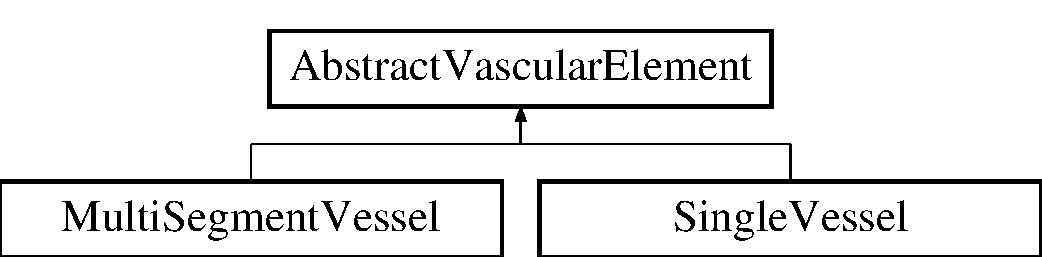
\includegraphics[height=2.000000cm]{d6/db2/class_abstract_vascular_element}
\end{center}
\end{figure}
\subsection*{Public Types}
\begin{DoxyCompactItemize}
\item 
enum \hyperlink{class_abstract_vascular_element_a9c7d6ae9fe8c220ddad143208b0a5a11}{T\+E\+R\+M\+I\+N\+A\+L\+\_\+\+T\+Y\+PE} \{ {\bfseries C\+O\+M\+M\+ON}, 
{\bfseries R\+E\+S\+E\+R\+V\+ED}
 \}
\item 
enum \hyperlink{class_abstract_vascular_element_a2f7b3a097b944cd0b056fee00b93c860}{B\+R\+A\+N\+C\+H\+I\+N\+G\+\_\+\+M\+O\+DE} \{ \\*
{\bfseries N\+O\+\_\+\+B\+R\+A\+N\+C\+H\+I\+NG}, 
{\bfseries R\+I\+G\+I\+D\+\_\+\+P\+A\+R\+E\+NT}, 
{\bfseries D\+E\+F\+O\+R\+M\+A\+B\+L\+E\+\_\+\+P\+A\+R\+E\+NT}, 
{\bfseries D\+I\+S\+T\+A\+L\+\_\+\+B\+R\+A\+N\+C\+H\+I\+NG}, 
\\*
{\bfseries O\+N\+L\+Y\+\_\+\+A\+T\+\_\+\+P\+A\+R\+E\+N\+T\+\_\+\+H\+O\+T\+S\+P\+O\+TS}
 \}
\item 
enum \hyperlink{class_abstract_vascular_element_a7d7b7863aae4952ba79a590ee65702ec}{V\+E\+S\+S\+E\+L\+\_\+\+F\+U\+N\+C\+T\+I\+ON} \{ {\bfseries D\+I\+S\+T\+R\+I\+B\+U\+T\+I\+ON}, 
{\bfseries P\+E\+R\+F\+O\+R\+A\+T\+OR}, 
{\bfseries T\+R\+A\+N\+S\+P\+O\+RT}
 \}
\end{DoxyCompactItemize}
\subsection*{Public Member Functions}
\begin{DoxyCompactItemize}
\item 
\hyperlink{class_abstract_vascular_element_af7280c0e7e9761f70a9dc556a51dd486}{Abstract\+Vascular\+Element} ()
\item 
virtual \hyperlink{class_abstract_vascular_element_ab5b056a128b4a72707070af67f5960ce}{$\sim$\+Abstract\+Vascular\+Element} ()
\item 
void \hyperlink{class_abstract_vascular_element_a9d5fd23d4e2cb02db821bc84ac3996e5}{set\+Branching\+Mode} (\hyperlink{class_abstract_vascular_element_a2f7b3a097b944cd0b056fee00b93c860}{B\+R\+A\+N\+C\+H\+I\+N\+G\+\_\+\+M\+O\+DE} mode)
\item 
virtual void \hyperlink{class_abstract_vascular_element_a0ec4dde7ce06f1d977d19b5a340eca52}{get\+Branching\+Points} (vector$<$ \hyperlink{structpoint}{point} $>$ $\ast$branching\+Points, \hyperlink{structpoint}{point} x\+New)=0
\item 
vector$<$ \hyperlink{class_single_vessel}{Single\+Vessel} $\ast$ $>$ \& \hyperlink{class_abstract_vascular_element_a07ae829d7cd20498629cb7b5bade2168}{get\+Vessels} ()
\item 
virtual \hyperlink{class_abstract_vascular_element}{Abstract\+Vascular\+Element} $\ast$ \hyperlink{class_abstract_vascular_element_aab59dfe7c6d4c846cb8f341727be8261}{get\+Parent} ()=0
\item 
virtual \hyperlink{class_single_vessel}{Single\+Vessel} $\ast$ \hyperlink{class_abstract_vascular_element_a4007ab14544d8fb5cacf5c610e9b0e5d}{get\+Parent\+Vessel\+To} (\hyperlink{structpoint}{point} xp)=0
\item 
virtual vector$<$ \hyperlink{class_abstract_vascular_element}{Abstract\+Vascular\+Element} $\ast$ $>$ \& \hyperlink{class_abstract_vascular_element_ae9cf2675f971fa470c74403c8b923f7d}{get\+Children} ()=0
\item 
void \hyperlink{class_abstract_vascular_element_a1ae7f338dcf49892e6be5dc77bae6359}{add\+Child} (\hyperlink{class_abstract_vascular_element}{Abstract\+Vascular\+Element} $\ast$new\+Child)
\item 
void \hyperlink{class_abstract_vascular_element_a1d2f7a213c823837e8a89adfff71ce0d}{remove\+Children} ()
\item 
virtual vector$<$ \hyperlink{class_single_vessel}{Single\+Vessel} $\ast$ $>$ $\ast$ \hyperlink{class_abstract_vascular_element_aac4f9650c704d920903c49270b18f717}{get\+Children\+Vessel\+To} (\hyperlink{structpoint}{point} xd)=0
\item 
virtual vector$<$ \hyperlink{class_single_vessel}{Single\+Vessel} $\ast$ $>$ $\ast$ \hyperlink{class_abstract_vascular_element_a7720067153a223d373c26e14155553e3}{get\+Vessels\+Connected\+To} (\hyperlink{structpoint}{point} p)=0
\item 
virtual long long int \hyperlink{class_abstract_vascular_element_a85d8d19d6f92a4e7cc95cc0f8f5a59c9}{get\+Terminals} ()=0
\item 
virtual long long int {\bfseries get\+Terminals} (\hyperlink{class_abstract_vascular_element_a9c7d6ae9fe8c220ddad143208b0a5a11}{T\+E\+R\+M\+I\+N\+A\+L\+\_\+\+T\+Y\+PE} type)=0\hypertarget{class_abstract_vascular_element_a78601a0007b77be084b381834a9e20e4}{}\label{class_abstract_vascular_element_a78601a0007b77be084b381834a9e20e4}

\item 
virtual double \hyperlink{class_abstract_vascular_element_ae4ecb632a94e89ac21f6523637bdb9cd}{get\+Volume} ()=0
\item 
virtual void \hyperlink{class_abstract_vascular_element_a258a830359614d0217e820293a9bdaa9}{update\+Pressure} ()=0
\item 
virtual double \hyperlink{class_abstract_vascular_element_a3880bed8d0a9223107bcee195bb89e51}{get\+Distal\+Radius} ()=0
\item 
virtual double \hyperlink{class_abstract_vascular_element_aa486370af563a9ea9bfcdcde8ee38426}{get\+Proximal\+Pressure} ()=0
\item 
virtual void \hyperlink{class_abstract_vascular_element_aff5f129b31f0c82aebf2d7387859914d}{save\+Vessel\+Data} (ofstream $\ast$tree\+File)=0
\item 
virtual void \hyperlink{class_abstract_vascular_element_a878c2826beb1a549c28659182760fbab}{save\+Vessel\+Connectivity} (ofstream $\ast$tree\+File)=0
\end{DoxyCompactItemize}
\subsection*{Public Attributes}
\begin{DoxyCompactItemize}
\item 
\hyperlink{class_abstract_vascular_element_a9c7d6ae9fe8c220ddad143208b0a5a11}{T\+E\+R\+M\+I\+N\+A\+L\+\_\+\+T\+Y\+PE} \hyperlink{class_abstract_vascular_element_a334fcc3576ed763aee815e8930251b94}{terminal\+Type}
\item 
double \hyperlink{class_abstract_vascular_element_a6137eb31a060a8806a44204b421d074f}{q\+Reserved\+Fraction}
\item 
int \hyperlink{class_abstract_vascular_element_a8a9351cffd2ca12dd531ab10fcd01b81}{stage}
\item 
\hyperlink{class_abstract_vascular_element}{Abstract\+Vascular\+Element} $\ast$ \hyperlink{class_abstract_vascular_element_aa43cbab70a108afebfdacd3e8a181b38}{parent}
\item 
vector$<$ \hyperlink{class_abstract_vascular_element}{Abstract\+Vascular\+Element} $\ast$ $>$ \hyperlink{class_abstract_vascular_element_a4f960c758678631f7a046b7becfe021b}{children}
\item 
\hyperlink{class_abstract_vascular_element_a2f7b3a097b944cd0b056fee00b93c860}{B\+R\+A\+N\+C\+H\+I\+N\+G\+\_\+\+M\+O\+DE} \hyperlink{class_abstract_vascular_element_a3bd09108bf46c95f5cf790e910744cd1}{branching\+Mode}
\item 
\hyperlink{class_abstract_vascular_element_a7d7b7863aae4952ba79a590ee65702ec}{V\+E\+S\+S\+E\+L\+\_\+\+F\+U\+N\+C\+T\+I\+ON} \hyperlink{class_abstract_vascular_element_a4d207777a63223377e3a8b69c50c2a08}{vessel\+Function}
\end{DoxyCompactItemize}
\subsection*{Protected Attributes}
\begin{DoxyCompactItemize}
\item 
vector$<$ \hyperlink{class_single_vessel}{Single\+Vessel} $\ast$ $>$ \hyperlink{class_abstract_vascular_element_ace778eb36210480ccfbaadfcd8c4802b}{vessels}
\end{DoxyCompactItemize}


\subsection{Detailed Description}
Abstract vascular element that can be composed by a set of vessels. 

\subsection{Member Enumeration Documentation}
\index{Abstract\+Vascular\+Element@{Abstract\+Vascular\+Element}!B\+R\+A\+N\+C\+H\+I\+N\+G\+\_\+\+M\+O\+DE@{B\+R\+A\+N\+C\+H\+I\+N\+G\+\_\+\+M\+O\+DE}}
\index{B\+R\+A\+N\+C\+H\+I\+N\+G\+\_\+\+M\+O\+DE@{B\+R\+A\+N\+C\+H\+I\+N\+G\+\_\+\+M\+O\+DE}!Abstract\+Vascular\+Element@{Abstract\+Vascular\+Element}}
\subsubsection[{\texorpdfstring{B\+R\+A\+N\+C\+H\+I\+N\+G\+\_\+\+M\+O\+DE}{BRANCHING_MODE}}]{\setlength{\rightskip}{0pt plus 5cm}enum {\bf Abstract\+Vascular\+Element\+::\+B\+R\+A\+N\+C\+H\+I\+N\+G\+\_\+\+M\+O\+DE}}\hypertarget{class_abstract_vascular_element_a2f7b3a097b944cd0b056fee00b93c860}{}\label{class_abstract_vascular_element_a2f7b3a097b944cd0b056fee00b93c860}
Indicates how and where this vessel can branch when it is parent. \index{Abstract\+Vascular\+Element@{Abstract\+Vascular\+Element}!T\+E\+R\+M\+I\+N\+A\+L\+\_\+\+T\+Y\+PE@{T\+E\+R\+M\+I\+N\+A\+L\+\_\+\+T\+Y\+PE}}
\index{T\+E\+R\+M\+I\+N\+A\+L\+\_\+\+T\+Y\+PE@{T\+E\+R\+M\+I\+N\+A\+L\+\_\+\+T\+Y\+PE}!Abstract\+Vascular\+Element@{Abstract\+Vascular\+Element}}
\subsubsection[{\texorpdfstring{T\+E\+R\+M\+I\+N\+A\+L\+\_\+\+T\+Y\+PE}{TERMINAL_TYPE}}]{\setlength{\rightskip}{0pt plus 5cm}enum {\bf Abstract\+Vascular\+Element\+::\+T\+E\+R\+M\+I\+N\+A\+L\+\_\+\+T\+Y\+PE}}\hypertarget{class_abstract_vascular_element_a9c7d6ae9fe8c220ddad143208b0a5a11}{}\label{class_abstract_vascular_element_a9c7d6ae9fe8c220ddad143208b0a5a11}
Indicates the behavior of the terminal for flow distribution. \index{Abstract\+Vascular\+Element@{Abstract\+Vascular\+Element}!V\+E\+S\+S\+E\+L\+\_\+\+F\+U\+N\+C\+T\+I\+ON@{V\+E\+S\+S\+E\+L\+\_\+\+F\+U\+N\+C\+T\+I\+ON}}
\index{V\+E\+S\+S\+E\+L\+\_\+\+F\+U\+N\+C\+T\+I\+ON@{V\+E\+S\+S\+E\+L\+\_\+\+F\+U\+N\+C\+T\+I\+ON}!Abstract\+Vascular\+Element@{Abstract\+Vascular\+Element}}
\subsubsection[{\texorpdfstring{V\+E\+S\+S\+E\+L\+\_\+\+F\+U\+N\+C\+T\+I\+ON}{VESSEL_FUNCTION}}]{\setlength{\rightskip}{0pt plus 5cm}enum {\bf Abstract\+Vascular\+Element\+::\+V\+E\+S\+S\+E\+L\+\_\+\+F\+U\+N\+C\+T\+I\+ON}}\hypertarget{class_abstract_vascular_element_a7d7b7863aae4952ba79a590ee65702ec}{}\label{class_abstract_vascular_element_a7d7b7863aae4952ba79a590ee65702ec}
Indicates the vessel function that constraints where it can bifurcates. Perforators may bifurcates while they are partially outside the domain, but its partition point must be inside the domain. Transport vessels bifurcates outside the domain and distribution vessels bifurcates inside the domain. 

\subsection{Constructor \& Destructor Documentation}
\index{Abstract\+Vascular\+Element@{Abstract\+Vascular\+Element}!Abstract\+Vascular\+Element@{Abstract\+Vascular\+Element}}
\index{Abstract\+Vascular\+Element@{Abstract\+Vascular\+Element}!Abstract\+Vascular\+Element@{Abstract\+Vascular\+Element}}
\subsubsection[{\texorpdfstring{Abstract\+Vascular\+Element()}{AbstractVascularElement()}}]{\setlength{\rightskip}{0pt plus 5cm}Abstract\+Vascular\+Element\+::\+Abstract\+Vascular\+Element (
\begin{DoxyParamCaption}
{}
\end{DoxyParamCaption}
)}\hypertarget{class_abstract_vascular_element_af7280c0e7e9761f70a9dc556a51dd486}{}\label{class_abstract_vascular_element_af7280c0e7e9761f70a9dc556a51dd486}
Common constructor. \index{Abstract\+Vascular\+Element@{Abstract\+Vascular\+Element}!````~Abstract\+Vascular\+Element@{$\sim$\+Abstract\+Vascular\+Element}}
\index{````~Abstract\+Vascular\+Element@{$\sim$\+Abstract\+Vascular\+Element}!Abstract\+Vascular\+Element@{Abstract\+Vascular\+Element}}
\subsubsection[{\texorpdfstring{$\sim$\+Abstract\+Vascular\+Element()}{~AbstractVascularElement()}}]{\setlength{\rightskip}{0pt plus 5cm}Abstract\+Vascular\+Element\+::$\sim$\+Abstract\+Vascular\+Element (
\begin{DoxyParamCaption}
{}
\end{DoxyParamCaption}
)\hspace{0.3cm}{\ttfamily [virtual]}}\hypertarget{class_abstract_vascular_element_ab5b056a128b4a72707070af67f5960ce}{}\label{class_abstract_vascular_element_ab5b056a128b4a72707070af67f5960ce}
Destructor constructor. 

\subsection{Member Function Documentation}
\index{Abstract\+Vascular\+Element@{Abstract\+Vascular\+Element}!add\+Child@{add\+Child}}
\index{add\+Child@{add\+Child}!Abstract\+Vascular\+Element@{Abstract\+Vascular\+Element}}
\subsubsection[{\texorpdfstring{add\+Child(\+Abstract\+Vascular\+Element $\ast$new\+Child)}{addChild(AbstractVascularElement *newChild)}}]{\setlength{\rightskip}{0pt plus 5cm}void Abstract\+Vascular\+Element\+::add\+Child (
\begin{DoxyParamCaption}
\item[{{\bf Abstract\+Vascular\+Element} $\ast$}]{new\+Child}
\end{DoxyParamCaption}
)}\hypertarget{class_abstract_vascular_element_a1ae7f338dcf49892e6be5dc77bae6359}{}\label{class_abstract_vascular_element_a1ae7f338dcf49892e6be5dc77bae6359}
Adds a new child to the children vector. 
\begin{DoxyParams}{Parameters}
{\em new\+Child} & New child to be inserted in the structure. \\
\hline
\end{DoxyParams}
\index{Abstract\+Vascular\+Element@{Abstract\+Vascular\+Element}!get\+Branching\+Points@{get\+Branching\+Points}}
\index{get\+Branching\+Points@{get\+Branching\+Points}!Abstract\+Vascular\+Element@{Abstract\+Vascular\+Element}}
\subsubsection[{\texorpdfstring{get\+Branching\+Points(vector$<$ point $>$ $\ast$branching\+Points, point x\+New)=0}{getBranchingPoints(vector< point > *branchingPoints, point xNew)=0}}]{\setlength{\rightskip}{0pt plus 5cm}virtual void Abstract\+Vascular\+Element\+::get\+Branching\+Points (
\begin{DoxyParamCaption}
\item[{vector$<$ {\bf point} $>$ $\ast$}]{branching\+Points, }
\item[{{\bf point}}]{x\+New}
\end{DoxyParamCaption}
)\hspace{0.3cm}{\ttfamily [pure virtual]}}\hypertarget{class_abstract_vascular_element_a0ec4dde7ce06f1d977d19b5a340eca52}{}\label{class_abstract_vascular_element_a0ec4dde7ce06f1d977d19b5a340eca52}
Fill {\ttfamily branching\+Points} with the potential points for branching in the current vessel, accorading to the {\ttfamily branching\+Mode}. 
\begin{DoxyParams}{Parameters}
{\em branching\+Points} & Vector filled with the possible branching points of this vessel. \\
\hline
\end{DoxyParams}


Implemented in \hyperlink{class_single_vessel_a6e397458482fd04bc3c1514eb518f05b}{Single\+Vessel}.

\index{Abstract\+Vascular\+Element@{Abstract\+Vascular\+Element}!get\+Children@{get\+Children}}
\index{get\+Children@{get\+Children}!Abstract\+Vascular\+Element@{Abstract\+Vascular\+Element}}
\subsubsection[{\texorpdfstring{get\+Children()=0}{getChildren()=0}}]{\setlength{\rightskip}{0pt plus 5cm}virtual vector$<${\bf Abstract\+Vascular\+Element} $\ast$$>$\& Abstract\+Vascular\+Element\+::get\+Children (
\begin{DoxyParamCaption}
{}
\end{DoxyParamCaption}
)\hspace{0.3cm}{\ttfamily [pure virtual]}}\hypertarget{class_abstract_vascular_element_ae9cf2675f971fa470c74403c8b923f7d}{}\label{class_abstract_vascular_element_ae9cf2675f971fa470c74403c8b923f7d}
Returns all the children vessels to this vascular element. \begin{DoxyReturn}{Returns}
Children vessels to this vascular element. 
\end{DoxyReturn}


Implemented in \hyperlink{class_single_vessel_a982d61ce4b6025bc07a4ccc95e1acc9f}{Single\+Vessel}, and \hyperlink{class_multi_segment_vessel_a1822f40db542ad537c16499ca47ae09d}{Multi\+Segment\+Vessel}.

\index{Abstract\+Vascular\+Element@{Abstract\+Vascular\+Element}!get\+Children\+Vessel\+To@{get\+Children\+Vessel\+To}}
\index{get\+Children\+Vessel\+To@{get\+Children\+Vessel\+To}!Abstract\+Vascular\+Element@{Abstract\+Vascular\+Element}}
\subsubsection[{\texorpdfstring{get\+Children\+Vessel\+To(point xd)=0}{getChildrenVesselTo(point xd)=0}}]{\setlength{\rightskip}{0pt plus 5cm}virtual vector$<${\bf Single\+Vessel}$\ast$$>$$\ast$ Abstract\+Vascular\+Element\+::get\+Children\+Vessel\+To (
\begin{DoxyParamCaption}
\item[{{\bf point}}]{xd}
\end{DoxyParamCaption}
)\hspace{0.3cm}{\ttfamily [pure virtual]}}\hypertarget{class_abstract_vascular_element_aac4f9650c704d920903c49270b18f717}{}\label{class_abstract_vascular_element_aac4f9650c704d920903c49270b18f717}
Returns all \hyperlink{class_single_vessel}{Single\+Vessel} that are children of this vascular element. 
\begin{DoxyParams}{Parameters}
{\em xd} & Point of children vessels attachment. \\
\hline
\end{DoxyParams}
\begin{DoxyReturn}{Returns}
\hyperlink{class_single_vessel}{Single\+Vessel} that is parent for this vascular element. 
\end{DoxyReturn}


Implemented in \hyperlink{class_single_vessel_a159e7d2d69cd3cae7b26f2ca374da817}{Single\+Vessel}, and \hyperlink{class_multi_segment_vessel_ad3220cc4fa66f851fd18b6126b250f1e}{Multi\+Segment\+Vessel}.

\index{Abstract\+Vascular\+Element@{Abstract\+Vascular\+Element}!get\+Distal\+Radius@{get\+Distal\+Radius}}
\index{get\+Distal\+Radius@{get\+Distal\+Radius}!Abstract\+Vascular\+Element@{Abstract\+Vascular\+Element}}
\subsubsection[{\texorpdfstring{get\+Distal\+Radius()=0}{getDistalRadius()=0}}]{\setlength{\rightskip}{0pt plus 5cm}virtual double Abstract\+Vascular\+Element\+::get\+Distal\+Radius (
\begin{DoxyParamCaption}
{}
\end{DoxyParamCaption}
)\hspace{0.3cm}{\ttfamily [pure virtual]}}\hypertarget{class_abstract_vascular_element_a3880bed8d0a9223107bcee195bb89e51}{}\label{class_abstract_vascular_element_a3880bed8d0a9223107bcee195bb89e51}
Returns the radius at the distal point of the vessel. \begin{DoxyReturn}{Returns}
Radius at the distal point of the vessel. 
\end{DoxyReturn}


Implemented in \hyperlink{class_single_vessel_a934c1d6b9a590621d53d78fedfed4c30}{Single\+Vessel}, and \hyperlink{class_multi_segment_vessel_ad0decc5c09f2ef4e58db122b4c511a65}{Multi\+Segment\+Vessel}.

\index{Abstract\+Vascular\+Element@{Abstract\+Vascular\+Element}!get\+Parent@{get\+Parent}}
\index{get\+Parent@{get\+Parent}!Abstract\+Vascular\+Element@{Abstract\+Vascular\+Element}}
\subsubsection[{\texorpdfstring{get\+Parent()=0}{getParent()=0}}]{\setlength{\rightskip}{0pt plus 5cm}virtual {\bf Abstract\+Vascular\+Element}$\ast$ Abstract\+Vascular\+Element\+::get\+Parent (
\begin{DoxyParamCaption}
{}
\end{DoxyParamCaption}
)\hspace{0.3cm}{\ttfamily [pure virtual]}}\hypertarget{class_abstract_vascular_element_aab59dfe7c6d4c846cb8f341727be8261}{}\label{class_abstract_vascular_element_aab59dfe7c6d4c846cb8f341727be8261}
Returns its parental \hyperlink{class_abstract_vascular_element}{Abstract\+Vascular\+Element}. \begin{DoxyReturn}{Returns}
\hyperlink{class_abstract_vascular_element}{Abstract\+Vascular\+Element} proximally attached. 
\end{DoxyReturn}


Implemented in \hyperlink{class_single_vessel_a7b905db74d4f733ea3cdb86ec961e9d1}{Single\+Vessel}, and \hyperlink{class_multi_segment_vessel_acd12912a043c6c28ede419ab2f65d77f}{Multi\+Segment\+Vessel}.

\index{Abstract\+Vascular\+Element@{Abstract\+Vascular\+Element}!get\+Parent\+Vessel\+To@{get\+Parent\+Vessel\+To}}
\index{get\+Parent\+Vessel\+To@{get\+Parent\+Vessel\+To}!Abstract\+Vascular\+Element@{Abstract\+Vascular\+Element}}
\subsubsection[{\texorpdfstring{get\+Parent\+Vessel\+To(point xp)=0}{getParentVesselTo(point xp)=0}}]{\setlength{\rightskip}{0pt plus 5cm}virtual {\bf Single\+Vessel}$\ast$ Abstract\+Vascular\+Element\+::get\+Parent\+Vessel\+To (
\begin{DoxyParamCaption}
\item[{{\bf point}}]{xp}
\end{DoxyParamCaption}
)\hspace{0.3cm}{\ttfamily [pure virtual]}}\hypertarget{class_abstract_vascular_element_a4007ab14544d8fb5cacf5c610e9b0e5d}{}\label{class_abstract_vascular_element_a4007ab14544d8fb5cacf5c610e9b0e5d}
Returns the \hyperlink{class_single_vessel}{Single\+Vessel} that is parent for this vascular element. 
\begin{DoxyParams}{Parameters}
{\em xp} & Point of parent vessel attachment. \\
\hline
\end{DoxyParams}
\begin{DoxyReturn}{Returns}
\hyperlink{class_single_vessel}{Single\+Vessel} that is parent for this vascular element. 
\end{DoxyReturn}


Implemented in \hyperlink{class_single_vessel_a25b7df0247aea7a482566de82c56ff3f}{Single\+Vessel}, and \hyperlink{class_multi_segment_vessel_a3c2b7f69de853adfb6434c4e5566bea6}{Multi\+Segment\+Vessel}.

\index{Abstract\+Vascular\+Element@{Abstract\+Vascular\+Element}!get\+Proximal\+Pressure@{get\+Proximal\+Pressure}}
\index{get\+Proximal\+Pressure@{get\+Proximal\+Pressure}!Abstract\+Vascular\+Element@{Abstract\+Vascular\+Element}}
\subsubsection[{\texorpdfstring{get\+Proximal\+Pressure()=0}{getProximalPressure()=0}}]{\setlength{\rightskip}{0pt plus 5cm}virtual double Abstract\+Vascular\+Element\+::get\+Proximal\+Pressure (
\begin{DoxyParamCaption}
{}
\end{DoxyParamCaption}
)\hspace{0.3cm}{\ttfamily [pure virtual]}}\hypertarget{class_abstract_vascular_element_aa486370af563a9ea9bfcdcde8ee38426}{}\label{class_abstract_vascular_element_aa486370af563a9ea9bfcdcde8ee38426}
Returns the pressure at the proximal point of the vessel. \begin{DoxyReturn}{Returns}
Pressure at the proximal point of the vessel. 
\end{DoxyReturn}


Implemented in \hyperlink{class_single_vessel_a439762c206fe749024ecc8c601d51738}{Single\+Vessel}, and \hyperlink{class_multi_segment_vessel_a8617911dd4618bc9d75a27c894f8b66d}{Multi\+Segment\+Vessel}.

\index{Abstract\+Vascular\+Element@{Abstract\+Vascular\+Element}!get\+Terminals@{get\+Terminals}}
\index{get\+Terminals@{get\+Terminals}!Abstract\+Vascular\+Element@{Abstract\+Vascular\+Element}}
\subsubsection[{\texorpdfstring{get\+Terminals()=0}{getTerminals()=0}}]{\setlength{\rightskip}{0pt plus 5cm}virtual long long int Abstract\+Vascular\+Element\+::get\+Terminals (
\begin{DoxyParamCaption}
{}
\end{DoxyParamCaption}
)\hspace{0.3cm}{\ttfamily [pure virtual]}}\hypertarget{class_abstract_vascular_element_a85d8d19d6f92a4e7cc95cc0f8f5a59c9}{}\label{class_abstract_vascular_element_a85d8d19d6f92a4e7cc95cc0f8f5a59c9}
Returns all the inner terminals in the current vascular element. \begin{DoxyReturn}{Returns}
Terminals in the current vascular element. 
\end{DoxyReturn}


Implemented in \hyperlink{class_single_vessel_a91a1cfd8cae1063b268cf1794859a245}{Single\+Vessel}, and \hyperlink{class_multi_segment_vessel_a5772718a4790089807df7b0f46f44c33}{Multi\+Segment\+Vessel}.

\index{Abstract\+Vascular\+Element@{Abstract\+Vascular\+Element}!get\+Vessels@{get\+Vessels}}
\index{get\+Vessels@{get\+Vessels}!Abstract\+Vascular\+Element@{Abstract\+Vascular\+Element}}
\subsubsection[{\texorpdfstring{get\+Vessels()}{getVessels()}}]{\setlength{\rightskip}{0pt plus 5cm}vector$<$ {\bf Single\+Vessel} $\ast$ $>$ \& Abstract\+Vascular\+Element\+::get\+Vessels (
\begin{DoxyParamCaption}
{}
\end{DoxyParamCaption}
)}\hypertarget{class_abstract_vascular_element_a07ae829d7cd20498629cb7b5bade2168}{}\label{class_abstract_vascular_element_a07ae829d7cd20498629cb7b5bade2168}
Returns all vessels in the vascular element. \begin{DoxyReturn}{Returns}
Set of all vessels in the vascular element. 
\end{DoxyReturn}
\index{Abstract\+Vascular\+Element@{Abstract\+Vascular\+Element}!get\+Vessels\+Connected\+To@{get\+Vessels\+Connected\+To}}
\index{get\+Vessels\+Connected\+To@{get\+Vessels\+Connected\+To}!Abstract\+Vascular\+Element@{Abstract\+Vascular\+Element}}
\subsubsection[{\texorpdfstring{get\+Vessels\+Connected\+To(point p)=0}{getVesselsConnectedTo(point p)=0}}]{\setlength{\rightskip}{0pt plus 5cm}virtual vector$<${\bf Single\+Vessel}$\ast$$>$$\ast$ Abstract\+Vascular\+Element\+::get\+Vessels\+Connected\+To (
\begin{DoxyParamCaption}
\item[{{\bf point}}]{p}
\end{DoxyParamCaption}
)\hspace{0.3cm}{\ttfamily [pure virtual]}}\hypertarget{class_abstract_vascular_element_a7720067153a223d373c26e14155553e3}{}\label{class_abstract_vascular_element_a7720067153a223d373c26e14155553e3}
Returns all vessels in this vascular structure connected to point {\ttfamily p}. 
\begin{DoxyParams}{Parameters}
{\em p} & Point at which all target vessels are connected to. \\
\hline
\end{DoxyParams}
\begin{DoxyReturn}{Returns}
Set of vessels connected to {\ttfamily p}. 
\end{DoxyReturn}


Implemented in \hyperlink{class_single_vessel_a42b2be50278e2c5ffe63d013b17e9713}{Single\+Vessel}, and \hyperlink{class_multi_segment_vessel_a7bf7eb14c3dbacf7e6fe6f9f00537d11}{Multi\+Segment\+Vessel}.

\index{Abstract\+Vascular\+Element@{Abstract\+Vascular\+Element}!get\+Volume@{get\+Volume}}
\index{get\+Volume@{get\+Volume}!Abstract\+Vascular\+Element@{Abstract\+Vascular\+Element}}
\subsubsection[{\texorpdfstring{get\+Volume()=0}{getVolume()=0}}]{\setlength{\rightskip}{0pt plus 5cm}virtual double Abstract\+Vascular\+Element\+::get\+Volume (
\begin{DoxyParamCaption}
{}
\end{DoxyParamCaption}
)\hspace{0.3cm}{\ttfamily [pure virtual]}}\hypertarget{class_abstract_vascular_element_ae4ecb632a94e89ac21f6523637bdb9cd}{}\label{class_abstract_vascular_element_ae4ecb632a94e89ac21f6523637bdb9cd}
Returns the functional cost contribution of this vascular element. If any constraint --e.\+g. geometric constrains-- are violated the function must return I\+N\+F\+I\+N\+I\+TY. \begin{DoxyReturn}{Returns}
Functional cost contribution. 
\end{DoxyReturn}


Implemented in \hyperlink{class_single_vessel_ac2cb07695080b9c7c6da65a2d52e0a51}{Single\+Vessel}, and \hyperlink{class_multi_segment_vessel_a1fdd2d4ed3fdd4e8cc62d4db6c390a27}{Multi\+Segment\+Vessel}.

\index{Abstract\+Vascular\+Element@{Abstract\+Vascular\+Element}!remove\+Children@{remove\+Children}}
\index{remove\+Children@{remove\+Children}!Abstract\+Vascular\+Element@{Abstract\+Vascular\+Element}}
\subsubsection[{\texorpdfstring{remove\+Children()}{removeChildren()}}]{\setlength{\rightskip}{0pt plus 5cm}void Abstract\+Vascular\+Element\+::remove\+Children (
\begin{DoxyParamCaption}
{}
\end{DoxyParamCaption}
)}\hypertarget{class_abstract_vascular_element_a1d2f7a213c823837e8a89adfff71ce0d}{}\label{class_abstract_vascular_element_a1d2f7a213c823837e8a89adfff71ce0d}
Remove all children. \index{Abstract\+Vascular\+Element@{Abstract\+Vascular\+Element}!save\+Vessel\+Connectivity@{save\+Vessel\+Connectivity}}
\index{save\+Vessel\+Connectivity@{save\+Vessel\+Connectivity}!Abstract\+Vascular\+Element@{Abstract\+Vascular\+Element}}
\subsubsection[{\texorpdfstring{save\+Vessel\+Connectivity(ofstream $\ast$tree\+File)=0}{saveVesselConnectivity(ofstream *treeFile)=0}}]{\setlength{\rightskip}{0pt plus 5cm}virtual void Abstract\+Vascular\+Element\+::save\+Vessel\+Connectivity (
\begin{DoxyParamCaption}
\item[{ofstream $\ast$}]{tree\+File}
\end{DoxyParamCaption}
)\hspace{0.3cm}{\ttfamily [pure virtual]}}\hypertarget{class_abstract_vascular_element_a878c2826beb1a549c28659182760fbab}{}\label{class_abstract_vascular_element_a878c2826beb1a549c28659182760fbab}
Writes connectivity of this vessel at the file associated to {\ttfamily tree\+File} stream. 
\begin{DoxyParams}{Parameters}
{\em tree\+File} & Output file stream. \\
\hline
\end{DoxyParams}


Implemented in \hyperlink{class_single_vessel_a84bfe24d24716e35cc1b811eea2a6ec8}{Single\+Vessel}, and \hyperlink{class_multi_segment_vessel_abf6e7a21a7b57f770723050515f1bd00}{Multi\+Segment\+Vessel}.

\index{Abstract\+Vascular\+Element@{Abstract\+Vascular\+Element}!save\+Vessel\+Data@{save\+Vessel\+Data}}
\index{save\+Vessel\+Data@{save\+Vessel\+Data}!Abstract\+Vascular\+Element@{Abstract\+Vascular\+Element}}
\subsubsection[{\texorpdfstring{save\+Vessel\+Data(ofstream $\ast$tree\+File)=0}{saveVesselData(ofstream *treeFile)=0}}]{\setlength{\rightskip}{0pt plus 5cm}virtual void Abstract\+Vascular\+Element\+::save\+Vessel\+Data (
\begin{DoxyParamCaption}
\item[{ofstream $\ast$}]{tree\+File}
\end{DoxyParamCaption}
)\hspace{0.3cm}{\ttfamily [pure virtual]}}\hypertarget{class_abstract_vascular_element_aff5f129b31f0c82aebf2d7387859914d}{}\label{class_abstract_vascular_element_aff5f129b31f0c82aebf2d7387859914d}
Writes the vessel data at the file associated to {\ttfamily tree\+File} stream. 
\begin{DoxyParams}{Parameters}
{\em tree\+File} & Output file stream. \\
\hline
\end{DoxyParams}


Implemented in \hyperlink{class_single_vessel_a11c4b9cfc4248dafda09d6a3ab8a60c7}{Single\+Vessel}, and \hyperlink{class_multi_segment_vessel_a870497c0529f2af9722f1a4a3d9d874d}{Multi\+Segment\+Vessel}.

\index{Abstract\+Vascular\+Element@{Abstract\+Vascular\+Element}!set\+Branching\+Mode@{set\+Branching\+Mode}}
\index{set\+Branching\+Mode@{set\+Branching\+Mode}!Abstract\+Vascular\+Element@{Abstract\+Vascular\+Element}}
\subsubsection[{\texorpdfstring{set\+Branching\+Mode(\+B\+R\+A\+N\+C\+H\+I\+N\+G\+\_\+\+M\+O\+D\+E mode)}{setBranchingMode(BRANCHING_MODE mode)}}]{\setlength{\rightskip}{0pt plus 5cm}void Abstract\+Vascular\+Element\+::set\+Branching\+Mode (
\begin{DoxyParamCaption}
\item[{{\bf B\+R\+A\+N\+C\+H\+I\+N\+G\+\_\+\+M\+O\+DE}}]{mode}
\end{DoxyParamCaption}
)}\hypertarget{class_abstract_vascular_element_a9d5fd23d4e2cb02db821bc84ac3996e5}{}\label{class_abstract_vascular_element_a9d5fd23d4e2cb02db821bc84ac3996e5}
Sets the branching mode for the current vessel. 
\begin{DoxyParams}{Parameters}
{\em mode} & Branching mode. \\
\hline
\end{DoxyParams}
\index{Abstract\+Vascular\+Element@{Abstract\+Vascular\+Element}!update\+Pressure@{update\+Pressure}}
\index{update\+Pressure@{update\+Pressure}!Abstract\+Vascular\+Element@{Abstract\+Vascular\+Element}}
\subsubsection[{\texorpdfstring{update\+Pressure()=0}{updatePressure()=0}}]{\setlength{\rightskip}{0pt plus 5cm}virtual void Abstract\+Vascular\+Element\+::update\+Pressure (
\begin{DoxyParamCaption}
{}
\end{DoxyParamCaption}
)\hspace{0.3cm}{\ttfamily [pure virtual]}}\hypertarget{class_abstract_vascular_element_a258a830359614d0217e820293a9bdaa9}{}\label{class_abstract_vascular_element_a258a830359614d0217e820293a9bdaa9}
Updates vascular element pressure from children to parent direction. 

Implemented in \hyperlink{class_single_vessel_adb7b986bc0da45d0720caf08989e00ce}{Single\+Vessel}, and \hyperlink{class_multi_segment_vessel_acd4b8dde6418dda9eaf3748e6ccbd0f1}{Multi\+Segment\+Vessel}.



\subsection{Member Data Documentation}
\index{Abstract\+Vascular\+Element@{Abstract\+Vascular\+Element}!branching\+Mode@{branching\+Mode}}
\index{branching\+Mode@{branching\+Mode}!Abstract\+Vascular\+Element@{Abstract\+Vascular\+Element}}
\subsubsection[{\texorpdfstring{branching\+Mode}{branchingMode}}]{\setlength{\rightskip}{0pt plus 5cm}{\bf B\+R\+A\+N\+C\+H\+I\+N\+G\+\_\+\+M\+O\+DE} Abstract\+Vascular\+Element\+::branching\+Mode}\hypertarget{class_abstract_vascular_element_a3bd09108bf46c95f5cf790e910744cd1}{}\label{class_abstract_vascular_element_a3bd09108bf46c95f5cf790e910744cd1}
Indicates the hotspots where the vessel can bifurcate. \index{Abstract\+Vascular\+Element@{Abstract\+Vascular\+Element}!children@{children}}
\index{children@{children}!Abstract\+Vascular\+Element@{Abstract\+Vascular\+Element}}
\subsubsection[{\texorpdfstring{children}{children}}]{\setlength{\rightskip}{0pt plus 5cm}vector$<${\bf Abstract\+Vascular\+Element} $\ast$$>$ Abstract\+Vascular\+Element\+::children}\hypertarget{class_abstract_vascular_element_a4f960c758678631f7a046b7becfe021b}{}\label{class_abstract_vascular_element_a4f960c758678631f7a046b7becfe021b}
The children vascular structures. \index{Abstract\+Vascular\+Element@{Abstract\+Vascular\+Element}!parent@{parent}}
\index{parent@{parent}!Abstract\+Vascular\+Element@{Abstract\+Vascular\+Element}}
\subsubsection[{\texorpdfstring{parent}{parent}}]{\setlength{\rightskip}{0pt plus 5cm}{\bf Abstract\+Vascular\+Element}$\ast$ Abstract\+Vascular\+Element\+::parent}\hypertarget{class_abstract_vascular_element_aa43cbab70a108afebfdacd3e8a181b38}{}\label{class_abstract_vascular_element_aa43cbab70a108afebfdacd3e8a181b38}
Parent vascular structure. \index{Abstract\+Vascular\+Element@{Abstract\+Vascular\+Element}!q\+Reserved\+Fraction@{q\+Reserved\+Fraction}}
\index{q\+Reserved\+Fraction@{q\+Reserved\+Fraction}!Abstract\+Vascular\+Element@{Abstract\+Vascular\+Element}}
\subsubsection[{\texorpdfstring{q\+Reserved\+Fraction}{qReservedFraction}}]{\setlength{\rightskip}{0pt plus 5cm}double Abstract\+Vascular\+Element\+::q\+Reserved\+Fraction}\hypertarget{class_abstract_vascular_element_a6137eb31a060a8806a44204b421d074f}{}\label{class_abstract_vascular_element_a6137eb31a060a8806a44204b421d074f}
Fraction of the q\+Reserved assigned to this vessel. \index{Abstract\+Vascular\+Element@{Abstract\+Vascular\+Element}!stage@{stage}}
\index{stage@{stage}!Abstract\+Vascular\+Element@{Abstract\+Vascular\+Element}}
\subsubsection[{\texorpdfstring{stage}{stage}}]{\setlength{\rightskip}{0pt plus 5cm}int Abstract\+Vascular\+Element\+::stage}\hypertarget{class_abstract_vascular_element_a8a9351cffd2ca12dd531ab10fcd01b81}{}\label{class_abstract_vascular_element_a8a9351cffd2ca12dd531ab10fcd01b81}
Parent vascular structure. \index{Abstract\+Vascular\+Element@{Abstract\+Vascular\+Element}!terminal\+Type@{terminal\+Type}}
\index{terminal\+Type@{terminal\+Type}!Abstract\+Vascular\+Element@{Abstract\+Vascular\+Element}}
\subsubsection[{\texorpdfstring{terminal\+Type}{terminalType}}]{\setlength{\rightskip}{0pt plus 5cm}{\bf T\+E\+R\+M\+I\+N\+A\+L\+\_\+\+T\+Y\+PE} Abstract\+Vascular\+Element\+::terminal\+Type}\hypertarget{class_abstract_vascular_element_a334fcc3576ed763aee815e8930251b94}{}\label{class_abstract_vascular_element_a334fcc3576ed763aee815e8930251b94}
Indicates the behavior of the terminal for flow distribution. \index{Abstract\+Vascular\+Element@{Abstract\+Vascular\+Element}!vessel\+Function@{vessel\+Function}}
\index{vessel\+Function@{vessel\+Function}!Abstract\+Vascular\+Element@{Abstract\+Vascular\+Element}}
\subsubsection[{\texorpdfstring{vessel\+Function}{vesselFunction}}]{\setlength{\rightskip}{0pt plus 5cm}{\bf V\+E\+S\+S\+E\+L\+\_\+\+F\+U\+N\+C\+T\+I\+ON} Abstract\+Vascular\+Element\+::vessel\+Function}\hypertarget{class_abstract_vascular_element_a4d207777a63223377e3a8b69c50c2a08}{}\label{class_abstract_vascular_element_a4d207777a63223377e3a8b69c50c2a08}
Type of vessel function for the current vessel. \index{Abstract\+Vascular\+Element@{Abstract\+Vascular\+Element}!vessels@{vessels}}
\index{vessels@{vessels}!Abstract\+Vascular\+Element@{Abstract\+Vascular\+Element}}
\subsubsection[{\texorpdfstring{vessels}{vessels}}]{\setlength{\rightskip}{0pt plus 5cm}vector$<${\bf Single\+Vessel} $\ast$$>$ Abstract\+Vascular\+Element\+::vessels\hspace{0.3cm}{\ttfamily [protected]}}\hypertarget{class_abstract_vascular_element_ace778eb36210480ccfbaadfcd8c4802b}{}\label{class_abstract_vascular_element_ace778eb36210480ccfbaadfcd8c4802b}
Vessels that constitute the current vascular element. 

The documentation for this class was generated from the following files\+:\begin{DoxyCompactItemize}
\item 
structures/vascular\+Elements/Abstract\+Vascular\+Element.\+h\item 
structures/vascular\+Elements/Abstract\+Vascular\+Element.\+cpp\end{DoxyCompactItemize}

\hypertarget{class_abstract_vessel_filter}{}\section{Abstract\+Vessel\+Filter Class Reference}
\label{class_abstract_vessel_filter}\index{Abstract\+Vessel\+Filter@{Abstract\+Vessel\+Filter}}
Inheritance diagram for Abstract\+Vessel\+Filter\+:\begin{figure}[H]
\begin{center}
\leavevmode
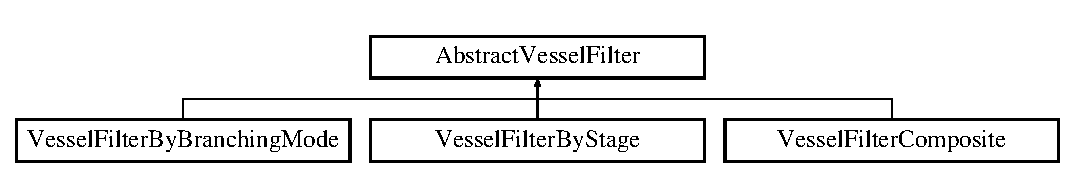
\includegraphics[height=1.944445cm]{d7/d7f/class_abstract_vessel_filter}
\end{center}
\end{figure}
\subsection*{Public Member Functions}
\begin{DoxyCompactItemize}
\item 
virtual vector$<$ \hyperlink{class_single_vessel}{Single\+Vessel} $\ast$ $>$ {\bfseries apply} (vector$<$ \hyperlink{class_single_vessel}{Single\+Vessel} $\ast$ $>$ vessels)=0\hypertarget{class_abstract_vessel_filter_ad73645d238d0eb0164897e8db7e211e7}{}\label{class_abstract_vessel_filter_ad73645d238d0eb0164897e8db7e211e7}

\end{DoxyCompactItemize}


The documentation for this class was generated from the following files\+:\begin{DoxyCompactItemize}
\item 
filters/Abstract\+Vessel\+Filter.\+h\item 
filters/Abstract\+Vessel\+Filter.\+cpp\end{DoxyCompactItemize}

\hypertarget{class_adim_sprouting_volumetric_cost_estimator}{}\section{Adim\+Sprouting\+Volumetric\+Cost\+Estimator Class Reference}
\label{class_adim_sprouting_volumetric_cost_estimator}\index{Adim\+Sprouting\+Volumetric\+Cost\+Estimator@{Adim\+Sprouting\+Volumetric\+Cost\+Estimator}}


{\ttfamily \#include $<$Adim\+Sprouting\+Volumetric\+Cost\+Estimator.\+h$>$}

Inheritance diagram for Adim\+Sprouting\+Volumetric\+Cost\+Estimator\+:\begin{figure}[H]
\begin{center}
\leavevmode
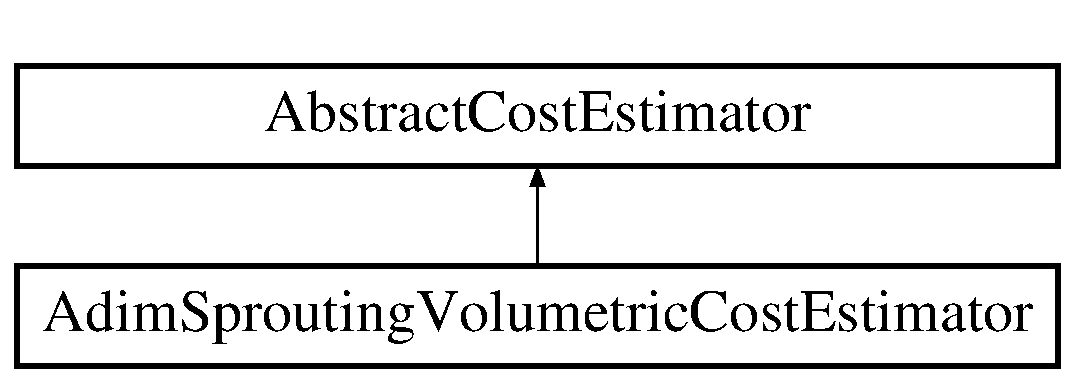
\includegraphics[height=2.000000cm]{dd/da2/class_adim_sprouting_volumetric_cost_estimator}
\end{center}
\end{figure}
\subsection*{Public Member Functions}
\begin{DoxyCompactItemize}
\item 
\hyperlink{class_adim_sprouting_volumetric_cost_estimator_a4c61439c00491a68093913ec96c0d41b}{Adim\+Sprouting\+Volumetric\+Cost\+Estimator} (double \hyperlink{class_adim_sprouting_volumetric_cost_estimator_a1d1ad71ae3bf8c56867108d30eba8091}{volume\+Factor}, double \hyperlink{class_adim_sprouting_volumetric_cost_estimator_ab8b8bfa47fa1e8283e9b1d9721d7cf29}{proteolytic\+Factor}, double \hyperlink{class_adim_sprouting_volumetric_cost_estimator_a1a4df5f80756f1559f76b8e980e48cf7}{diffusion\+Factor}, double \hyperlink{class_adim_sprouting_volumetric_cost_estimator_ac04ce5ad212cc71e3de3c3d3563217a2}{volume\+Ref}, double \hyperlink{class_adim_sprouting_volumetric_cost_estimator_a8d3cdcd6ecf322c066cd6042279af68c}{radius\+Ref})
\item 
virtual \hyperlink{class_adim_sprouting_volumetric_cost_estimator_a630e63baaff78716b56d5a35f393db93}{$\sim$\+Adim\+Sprouting\+Volumetric\+Cost\+Estimator} ()
\item 
\hyperlink{class_abstract_cost_estimator}{Abstract\+Cost\+Estimator} $\ast$ \hyperlink{class_adim_sprouting_volumetric_cost_estimator_acc28ad0a4add66222f87d9df84797524}{clone} ()
\item 
void \hyperlink{class_adim_sprouting_volumetric_cost_estimator_aa776aae78d397d422ff6b8041c07c412}{previous\+State} (\hyperlink{class_abstract_object_c_c_o_tree}{Abstract\+Object\+C\+C\+O\+Tree} $\ast$tree, \hyperlink{class_abstract_vascular_element}{Abstract\+Vascular\+Element} $\ast$parent, \hyperlink{structpoint}{point} i\+New, \hyperlink{structpoint}{point} i\+Test, double \hyperlink{class_adim_sprouting_volumetric_cost_estimator_a1b79ece84388a541810e55879ee99d8a}{d\+Lim})
\item 
double \hyperlink{class_adim_sprouting_volumetric_cost_estimator_a14757be74a1c73be8322dab990713936}{compute\+Cost} (\hyperlink{class_abstract_object_c_c_o_tree}{Abstract\+Object\+C\+C\+O\+Tree} $\ast$tree)
\end{DoxyCompactItemize}
\subsection*{Private Member Functions}
\begin{DoxyCompactItemize}
\item 
double \hyperlink{class_adim_sprouting_volumetric_cost_estimator_ac89ef88c033473f3dbc3209ae7fa79b1}{compute\+Tree\+Cost} (\hyperlink{class_abstract_vascular_element}{Abstract\+Vascular\+Element} $\ast$root)
\end{DoxyCompactItemize}
\subsection*{Private Attributes}
\begin{DoxyCompactItemize}
\item 
double \hyperlink{class_adim_sprouting_volumetric_cost_estimator_abcacf4498f7210da6ff4f04cca3ab176}{previous\+Volume}
\item 
double \hyperlink{class_adim_sprouting_volumetric_cost_estimator_ab8b8bfa47fa1e8283e9b1d9721d7cf29}{proteolytic\+Factor}
\item 
double \hyperlink{class_adim_sprouting_volumetric_cost_estimator_a1a4df5f80756f1559f76b8e980e48cf7}{diffusion\+Factor}
\item 
double \hyperlink{class_adim_sprouting_volumetric_cost_estimator_a1d1ad71ae3bf8c56867108d30eba8091}{volume\+Factor}
\item 
double \hyperlink{class_adim_sprouting_volumetric_cost_estimator_aab34b0032a1dd58352bce32596c6925c}{dist\+To\+Parent}
\item 
double \hyperlink{class_adim_sprouting_volumetric_cost_estimator_aecf10c7e6f390a23a1c6efdde6860a09}{parent\+Radius}
\item 
double \hyperlink{class_adim_sprouting_volumetric_cost_estimator_a1b79ece84388a541810e55879ee99d8a}{d\+Lim}
\item 
double \hyperlink{class_adim_sprouting_volumetric_cost_estimator_a04c0ad4a538a899e3b308a817348ce0f}{bif\+Level}
\item 
double \hyperlink{class_adim_sprouting_volumetric_cost_estimator_ac04ce5ad212cc71e3de3c3d3563217a2}{volume\+Ref}
\item 
double \hyperlink{class_adim_sprouting_volumetric_cost_estimator_a8d3cdcd6ecf322c066cd6042279af68c}{radius\+Ref}
\item 
double \hyperlink{class_adim_sprouting_volumetric_cost_estimator_a10b777646a17f717f48d81287f01863d}{length\+Ref}
\end{DoxyCompactItemize}


\subsection{Detailed Description}
Cost estimator that considers diffusion and vessel-\/wall degradation associated to sprouting angiogenesis and also weighs the variation of the tree volume. Wall degradation is assumed linear w.\+r.\+t. vessel radius (under the assumption that vessel thickness is linear with vessel radius) and media diffusion of biosignals is assumed to follow Fick\textquotesingle{}s 2nd law. 

\subsection{Constructor \& Destructor Documentation}
\index{Adim\+Sprouting\+Volumetric\+Cost\+Estimator@{Adim\+Sprouting\+Volumetric\+Cost\+Estimator}!Adim\+Sprouting\+Volumetric\+Cost\+Estimator@{Adim\+Sprouting\+Volumetric\+Cost\+Estimator}}
\index{Adim\+Sprouting\+Volumetric\+Cost\+Estimator@{Adim\+Sprouting\+Volumetric\+Cost\+Estimator}!Adim\+Sprouting\+Volumetric\+Cost\+Estimator@{Adim\+Sprouting\+Volumetric\+Cost\+Estimator}}
\subsubsection[{\texorpdfstring{Adim\+Sprouting\+Volumetric\+Cost\+Estimator(double volume\+Factor, double proteolytic\+Factor, double diffusion\+Factor, double volume\+Ref, double radius\+Ref)}{AdimSproutingVolumetricCostEstimator(double volumeFactor, double proteolyticFactor, double diffusionFactor, double volumeRef, double radiusRef)}}]{\setlength{\rightskip}{0pt plus 5cm}Adim\+Sprouting\+Volumetric\+Cost\+Estimator\+::\+Adim\+Sprouting\+Volumetric\+Cost\+Estimator (
\begin{DoxyParamCaption}
\item[{double}]{volume\+Factor, }
\item[{double}]{proteolytic\+Factor, }
\item[{double}]{diffusion\+Factor, }
\item[{double}]{volume\+Ref, }
\item[{double}]{radius\+Ref}
\end{DoxyParamCaption}
)}\hypertarget{class_adim_sprouting_volumetric_cost_estimator_a4c61439c00491a68093913ec96c0d41b}{}\label{class_adim_sprouting_volumetric_cost_estimator_a4c61439c00491a68093913ec96c0d41b}
Common constructor. \index{Adim\+Sprouting\+Volumetric\+Cost\+Estimator@{Adim\+Sprouting\+Volumetric\+Cost\+Estimator}!````~Adim\+Sprouting\+Volumetric\+Cost\+Estimator@{$\sim$\+Adim\+Sprouting\+Volumetric\+Cost\+Estimator}}
\index{````~Adim\+Sprouting\+Volumetric\+Cost\+Estimator@{$\sim$\+Adim\+Sprouting\+Volumetric\+Cost\+Estimator}!Adim\+Sprouting\+Volumetric\+Cost\+Estimator@{Adim\+Sprouting\+Volumetric\+Cost\+Estimator}}
\subsubsection[{\texorpdfstring{$\sim$\+Adim\+Sprouting\+Volumetric\+Cost\+Estimator()}{~AdimSproutingVolumetricCostEstimator()}}]{\setlength{\rightskip}{0pt plus 5cm}Adim\+Sprouting\+Volumetric\+Cost\+Estimator\+::$\sim$\+Adim\+Sprouting\+Volumetric\+Cost\+Estimator (
\begin{DoxyParamCaption}
{}
\end{DoxyParamCaption}
)\hspace{0.3cm}{\ttfamily [virtual]}}\hypertarget{class_adim_sprouting_volumetric_cost_estimator_a630e63baaff78716b56d5a35f393db93}{}\label{class_adim_sprouting_volumetric_cost_estimator_a630e63baaff78716b56d5a35f393db93}
Common destructor. 

\subsection{Member Function Documentation}
\index{Adim\+Sprouting\+Volumetric\+Cost\+Estimator@{Adim\+Sprouting\+Volumetric\+Cost\+Estimator}!clone@{clone}}
\index{clone@{clone}!Adim\+Sprouting\+Volumetric\+Cost\+Estimator@{Adim\+Sprouting\+Volumetric\+Cost\+Estimator}}
\subsubsection[{\texorpdfstring{clone()}{clone()}}]{\setlength{\rightskip}{0pt plus 5cm}{\bf Abstract\+Cost\+Estimator} $\ast$ Adim\+Sprouting\+Volumetric\+Cost\+Estimator\+::clone (
\begin{DoxyParamCaption}
{}
\end{DoxyParamCaption}
)\hspace{0.3cm}{\ttfamily [virtual]}}\hypertarget{class_adim_sprouting_volumetric_cost_estimator_acc28ad0a4add66222f87d9df84797524}{}\label{class_adim_sprouting_volumetric_cost_estimator_acc28ad0a4add66222f87d9df84797524}
Clones the current estimator instance. \begin{DoxyReturn}{Returns}
Cloned instance. 
\end{DoxyReturn}


Implements \hyperlink{class_abstract_cost_estimator_a928e53418b17eb68c443e2a68fe5cbcf}{Abstract\+Cost\+Estimator}.

\index{Adim\+Sprouting\+Volumetric\+Cost\+Estimator@{Adim\+Sprouting\+Volumetric\+Cost\+Estimator}!compute\+Cost@{compute\+Cost}}
\index{compute\+Cost@{compute\+Cost}!Adim\+Sprouting\+Volumetric\+Cost\+Estimator@{Adim\+Sprouting\+Volumetric\+Cost\+Estimator}}
\subsubsection[{\texorpdfstring{compute\+Cost(\+Abstract\+Object\+C\+C\+O\+Tree $\ast$tree)}{computeCost(AbstractObjectCCOTree *tree)}}]{\setlength{\rightskip}{0pt plus 5cm}double Adim\+Sprouting\+Volumetric\+Cost\+Estimator\+::compute\+Cost (
\begin{DoxyParamCaption}
\item[{{\bf Abstract\+Object\+C\+C\+O\+Tree} $\ast$}]{tree}
\end{DoxyParamCaption}
)\hspace{0.3cm}{\ttfamily [virtual]}}\hypertarget{class_adim_sprouting_volumetric_cost_estimator_a14757be74a1c73be8322dab990713936}{}\label{class_adim_sprouting_volumetric_cost_estimator_a14757be74a1c73be8322dab990713936}
Computes the functional cost of the given tree. 
\begin{DoxyParams}{Parameters}
{\em root} & Root of the tree at the current step. \\
\hline
\end{DoxyParams}
\begin{DoxyReturn}{Returns}
Cost of the given tree. 
\end{DoxyReturn}


Implements \hyperlink{class_abstract_cost_estimator_a2be0c6cc4aa6a73110c75ad903af428e}{Abstract\+Cost\+Estimator}.

\index{Adim\+Sprouting\+Volumetric\+Cost\+Estimator@{Adim\+Sprouting\+Volumetric\+Cost\+Estimator}!compute\+Tree\+Cost@{compute\+Tree\+Cost}}
\index{compute\+Tree\+Cost@{compute\+Tree\+Cost}!Adim\+Sprouting\+Volumetric\+Cost\+Estimator@{Adim\+Sprouting\+Volumetric\+Cost\+Estimator}}
\subsubsection[{\texorpdfstring{compute\+Tree\+Cost(\+Abstract\+Vascular\+Element $\ast$root)}{computeTreeCost(AbstractVascularElement *root)}}]{\setlength{\rightskip}{0pt plus 5cm}double Adim\+Sprouting\+Volumetric\+Cost\+Estimator\+::compute\+Tree\+Cost (
\begin{DoxyParamCaption}
\item[{{\bf Abstract\+Vascular\+Element} $\ast$}]{root}
\end{DoxyParamCaption}
)\hspace{0.3cm}{\ttfamily [private]}}\hypertarget{class_adim_sprouting_volumetric_cost_estimator_ac89ef88c033473f3dbc3209ae7fa79b1}{}\label{class_adim_sprouting_volumetric_cost_estimator_ac89ef88c033473f3dbc3209ae7fa79b1}
Computes the volume for the tree with root {\ttfamily root}. 
\begin{DoxyParams}{Parameters}
{\em root} & Root of the tree. \\
\hline
\end{DoxyParams}
\begin{DoxyReturn}{Returns}
Volume of the tree. 
\end{DoxyReturn}
\index{Adim\+Sprouting\+Volumetric\+Cost\+Estimator@{Adim\+Sprouting\+Volumetric\+Cost\+Estimator}!previous\+State@{previous\+State}}
\index{previous\+State@{previous\+State}!Adim\+Sprouting\+Volumetric\+Cost\+Estimator@{Adim\+Sprouting\+Volumetric\+Cost\+Estimator}}
\subsubsection[{\texorpdfstring{previous\+State(\+Abstract\+Object\+C\+C\+O\+Tree $\ast$tree, Abstract\+Vascular\+Element $\ast$parent, point i\+New, point i\+Test, double d\+Lim)}{previousState(AbstractObjectCCOTree *tree, AbstractVascularElement *parent, point iNew, point iTest, double dLim)}}]{\setlength{\rightskip}{0pt plus 5cm}void Adim\+Sprouting\+Volumetric\+Cost\+Estimator\+::previous\+State (
\begin{DoxyParamCaption}
\item[{{\bf Abstract\+Object\+C\+C\+O\+Tree} $\ast$}]{tree, }
\item[{{\bf Abstract\+Vascular\+Element} $\ast$}]{parent, }
\item[{{\bf point}}]{i\+New, }
\item[{{\bf point}}]{i\+Test, }
\item[{double}]{d\+Lim}
\end{DoxyParamCaption}
)\hspace{0.3cm}{\ttfamily [virtual]}}\hypertarget{class_adim_sprouting_volumetric_cost_estimator_aa776aae78d397d422ff6b8041c07c412}{}\label{class_adim_sprouting_volumetric_cost_estimator_aa776aae78d397d422ff6b8041c07c412}
Extracts information of the tree at the previous step. 
\begin{DoxyParams}{Parameters}
{\em root} & Root of the tree at the previous step. \\
\hline
{\em parent} & Vascular element where the new vessel will be connected. \\
\hline
{\em i\+New} & Distal position of the new vessel. \\
\hline
{\em i\+Test} & Proximal position of the new vessel. \\
\hline
{\em d\+Lim} & Minimum radius distance from the new vessel to the tree. \\
\hline
\end{DoxyParams}


Implements \hyperlink{class_abstract_cost_estimator_a8a806c3e4537c6d4acc428b029fd60de}{Abstract\+Cost\+Estimator}.



\subsection{Member Data Documentation}
\index{Adim\+Sprouting\+Volumetric\+Cost\+Estimator@{Adim\+Sprouting\+Volumetric\+Cost\+Estimator}!bif\+Level@{bif\+Level}}
\index{bif\+Level@{bif\+Level}!Adim\+Sprouting\+Volumetric\+Cost\+Estimator@{Adim\+Sprouting\+Volumetric\+Cost\+Estimator}}
\subsubsection[{\texorpdfstring{bif\+Level}{bifLevel}}]{\setlength{\rightskip}{0pt plus 5cm}double Adim\+Sprouting\+Volumetric\+Cost\+Estimator\+::bif\+Level\hspace{0.3cm}{\ttfamily [private]}}\hypertarget{class_adim_sprouting_volumetric_cost_estimator_a04c0ad4a538a899e3b308a817348ce0f}{}\label{class_adim_sprouting_volumetric_cost_estimator_a04c0ad4a538a899e3b308a817348ce0f}
Level of bifurcation. \index{Adim\+Sprouting\+Volumetric\+Cost\+Estimator@{Adim\+Sprouting\+Volumetric\+Cost\+Estimator}!diffusion\+Factor@{diffusion\+Factor}}
\index{diffusion\+Factor@{diffusion\+Factor}!Adim\+Sprouting\+Volumetric\+Cost\+Estimator@{Adim\+Sprouting\+Volumetric\+Cost\+Estimator}}
\subsubsection[{\texorpdfstring{diffusion\+Factor}{diffusionFactor}}]{\setlength{\rightskip}{0pt plus 5cm}double Adim\+Sprouting\+Volumetric\+Cost\+Estimator\+::diffusion\+Factor\hspace{0.3cm}{\ttfamily [private]}}\hypertarget{class_adim_sprouting_volumetric_cost_estimator_a1a4df5f80756f1559f76b8e980e48cf7}{}\label{class_adim_sprouting_volumetric_cost_estimator_a1a4df5f80756f1559f76b8e980e48cf7}
Factor of media diffusion of angiogenic growth factors. \index{Adim\+Sprouting\+Volumetric\+Cost\+Estimator@{Adim\+Sprouting\+Volumetric\+Cost\+Estimator}!dist\+To\+Parent@{dist\+To\+Parent}}
\index{dist\+To\+Parent@{dist\+To\+Parent}!Adim\+Sprouting\+Volumetric\+Cost\+Estimator@{Adim\+Sprouting\+Volumetric\+Cost\+Estimator}}
\subsubsection[{\texorpdfstring{dist\+To\+Parent}{distToParent}}]{\setlength{\rightskip}{0pt plus 5cm}double Adim\+Sprouting\+Volumetric\+Cost\+Estimator\+::dist\+To\+Parent\hspace{0.3cm}{\ttfamily [private]}}\hypertarget{class_adim_sprouting_volumetric_cost_estimator_aab34b0032a1dd58352bce32596c6925c}{}\label{class_adim_sprouting_volumetric_cost_estimator_aab34b0032a1dd58352bce32596c6925c}
Distance between sprouting source and candidate parent vessel. \index{Adim\+Sprouting\+Volumetric\+Cost\+Estimator@{Adim\+Sprouting\+Volumetric\+Cost\+Estimator}!d\+Lim@{d\+Lim}}
\index{d\+Lim@{d\+Lim}!Adim\+Sprouting\+Volumetric\+Cost\+Estimator@{Adim\+Sprouting\+Volumetric\+Cost\+Estimator}}
\subsubsection[{\texorpdfstring{d\+Lim}{dLim}}]{\setlength{\rightskip}{0pt plus 5cm}double Adim\+Sprouting\+Volumetric\+Cost\+Estimator\+::d\+Lim\hspace{0.3cm}{\ttfamily [private]}}\hypertarget{class_adim_sprouting_volumetric_cost_estimator_a1b79ece84388a541810e55879ee99d8a}{}\label{class_adim_sprouting_volumetric_cost_estimator_a1b79ece84388a541810e55879ee99d8a}
Minimum radius distance from the new vessel to the tree. \index{Adim\+Sprouting\+Volumetric\+Cost\+Estimator@{Adim\+Sprouting\+Volumetric\+Cost\+Estimator}!length\+Ref@{length\+Ref}}
\index{length\+Ref@{length\+Ref}!Adim\+Sprouting\+Volumetric\+Cost\+Estimator@{Adim\+Sprouting\+Volumetric\+Cost\+Estimator}}
\subsubsection[{\texorpdfstring{length\+Ref}{lengthRef}}]{\setlength{\rightskip}{0pt plus 5cm}double Adim\+Sprouting\+Volumetric\+Cost\+Estimator\+::length\+Ref\hspace{0.3cm}{\ttfamily [private]}}\hypertarget{class_adim_sprouting_volumetric_cost_estimator_a10b777646a17f717f48d81287f01863d}{}\label{class_adim_sprouting_volumetric_cost_estimator_a10b777646a17f717f48d81287f01863d}
Equivalent radius associated to {\ttfamily v\+Ref} \index{Adim\+Sprouting\+Volumetric\+Cost\+Estimator@{Adim\+Sprouting\+Volumetric\+Cost\+Estimator}!parent\+Radius@{parent\+Radius}}
\index{parent\+Radius@{parent\+Radius}!Adim\+Sprouting\+Volumetric\+Cost\+Estimator@{Adim\+Sprouting\+Volumetric\+Cost\+Estimator}}
\subsubsection[{\texorpdfstring{parent\+Radius}{parentRadius}}]{\setlength{\rightskip}{0pt plus 5cm}double Adim\+Sprouting\+Volumetric\+Cost\+Estimator\+::parent\+Radius\hspace{0.3cm}{\ttfamily [private]}}\hypertarget{class_adim_sprouting_volumetric_cost_estimator_aecf10c7e6f390a23a1c6efdde6860a09}{}\label{class_adim_sprouting_volumetric_cost_estimator_aecf10c7e6f390a23a1c6efdde6860a09}
Radius of the candidate parent vessel. \index{Adim\+Sprouting\+Volumetric\+Cost\+Estimator@{Adim\+Sprouting\+Volumetric\+Cost\+Estimator}!previous\+Volume@{previous\+Volume}}
\index{previous\+Volume@{previous\+Volume}!Adim\+Sprouting\+Volumetric\+Cost\+Estimator@{Adim\+Sprouting\+Volumetric\+Cost\+Estimator}}
\subsubsection[{\texorpdfstring{previous\+Volume}{previousVolume}}]{\setlength{\rightskip}{0pt plus 5cm}double Adim\+Sprouting\+Volumetric\+Cost\+Estimator\+::previous\+Volume\hspace{0.3cm}{\ttfamily [private]}}\hypertarget{class_adim_sprouting_volumetric_cost_estimator_abcacf4498f7210da6ff4f04cca3ab176}{}\label{class_adim_sprouting_volumetric_cost_estimator_abcacf4498f7210da6ff4f04cca3ab176}
Volume at the previous step. \index{Adim\+Sprouting\+Volumetric\+Cost\+Estimator@{Adim\+Sprouting\+Volumetric\+Cost\+Estimator}!proteolytic\+Factor@{proteolytic\+Factor}}
\index{proteolytic\+Factor@{proteolytic\+Factor}!Adim\+Sprouting\+Volumetric\+Cost\+Estimator@{Adim\+Sprouting\+Volumetric\+Cost\+Estimator}}
\subsubsection[{\texorpdfstring{proteolytic\+Factor}{proteolyticFactor}}]{\setlength{\rightskip}{0pt plus 5cm}double Adim\+Sprouting\+Volumetric\+Cost\+Estimator\+::proteolytic\+Factor\hspace{0.3cm}{\ttfamily [private]}}\hypertarget{class_adim_sprouting_volumetric_cost_estimator_ab8b8bfa47fa1e8283e9b1d9721d7cf29}{}\label{class_adim_sprouting_volumetric_cost_estimator_ab8b8bfa47fa1e8283e9b1d9721d7cf29}
Vessel wall proteolytic degradation factor. \index{Adim\+Sprouting\+Volumetric\+Cost\+Estimator@{Adim\+Sprouting\+Volumetric\+Cost\+Estimator}!radius\+Ref@{radius\+Ref}}
\index{radius\+Ref@{radius\+Ref}!Adim\+Sprouting\+Volumetric\+Cost\+Estimator@{Adim\+Sprouting\+Volumetric\+Cost\+Estimator}}
\subsubsection[{\texorpdfstring{radius\+Ref}{radiusRef}}]{\setlength{\rightskip}{0pt plus 5cm}double Adim\+Sprouting\+Volumetric\+Cost\+Estimator\+::radius\+Ref\hspace{0.3cm}{\ttfamily [private]}}\hypertarget{class_adim_sprouting_volumetric_cost_estimator_a8d3cdcd6ecf322c066cd6042279af68c}{}\label{class_adim_sprouting_volumetric_cost_estimator_a8d3cdcd6ecf322c066cd6042279af68c}
Root radius of the vascular tree \index{Adim\+Sprouting\+Volumetric\+Cost\+Estimator@{Adim\+Sprouting\+Volumetric\+Cost\+Estimator}!volume\+Factor@{volume\+Factor}}
\index{volume\+Factor@{volume\+Factor}!Adim\+Sprouting\+Volumetric\+Cost\+Estimator@{Adim\+Sprouting\+Volumetric\+Cost\+Estimator}}
\subsubsection[{\texorpdfstring{volume\+Factor}{volumeFactor}}]{\setlength{\rightskip}{0pt plus 5cm}double Adim\+Sprouting\+Volumetric\+Cost\+Estimator\+::volume\+Factor\hspace{0.3cm}{\ttfamily [private]}}\hypertarget{class_adim_sprouting_volumetric_cost_estimator_a1d1ad71ae3bf8c56867108d30eba8091}{}\label{class_adim_sprouting_volumetric_cost_estimator_a1d1ad71ae3bf8c56867108d30eba8091}
Weigh for tree volume. \index{Adim\+Sprouting\+Volumetric\+Cost\+Estimator@{Adim\+Sprouting\+Volumetric\+Cost\+Estimator}!volume\+Ref@{volume\+Ref}}
\index{volume\+Ref@{volume\+Ref}!Adim\+Sprouting\+Volumetric\+Cost\+Estimator@{Adim\+Sprouting\+Volumetric\+Cost\+Estimator}}
\subsubsection[{\texorpdfstring{volume\+Ref}{volumeRef}}]{\setlength{\rightskip}{0pt plus 5cm}double Adim\+Sprouting\+Volumetric\+Cost\+Estimator\+::volume\+Ref\hspace{0.3cm}{\ttfamily [private]}}\hypertarget{class_adim_sprouting_volumetric_cost_estimator_ac04ce5ad212cc71e3de3c3d3563217a2}{}\label{class_adim_sprouting_volumetric_cost_estimator_ac04ce5ad212cc71e3de3c3d3563217a2}
Volume of the vascularized domain 

The documentation for this class was generated from the following files\+:\begin{DoxyCompactItemize}
\item 
structures/tree/Adim\+Sprouting\+Volumetric\+Cost\+Estimator.\+h\item 
structures/tree/Adim\+Sprouting\+Volumetric\+Cost\+Estimator.\+cpp\end{DoxyCompactItemize}

\hypertarget{class_checkpoint_saving_task}{}\section{Checkpoint\+Saving\+Task Class Reference}
\label{class_checkpoint_saving_task}\index{Checkpoint\+Saving\+Task@{Checkpoint\+Saving\+Task}}


{\ttfamily \#include $<$Checkpoint\+Saving\+Task.\+h$>$}

Inheritance diagram for Checkpoint\+Saving\+Task\+:\begin{figure}[H]
\begin{center}
\leavevmode
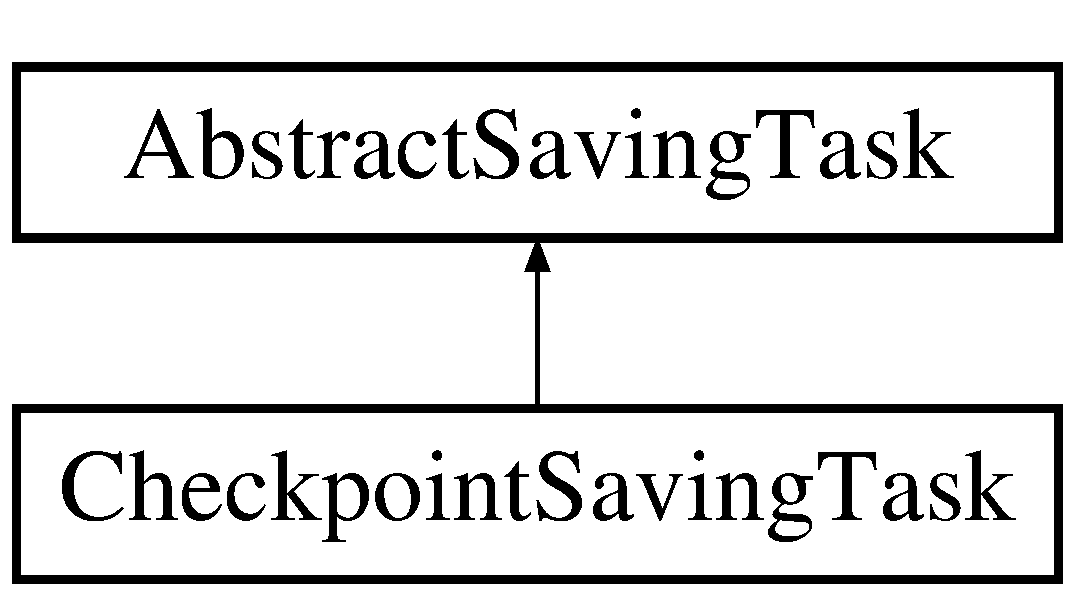
\includegraphics[height=2.000000cm]{d8/d08/class_checkpoint_saving_task}
\end{center}
\end{figure}
\subsection*{Public Member Functions}
\begin{DoxyCompactItemize}
\item 
\hyperlink{class_checkpoint_saving_task_aecde19cadd1ba092b96944eca86684f1}{Checkpoint\+Saving\+Task} (string path, string prefix, \hyperlink{class_single_vessel_c_c_o_o_tree}{Single\+Vessel\+C\+C\+O\+O\+Tree} $\ast$tree)
\item 
void \hyperlink{class_checkpoint_saving_task_a9c2ed33439fab8564b26e5b3396a8008}{execute} (long long int terminals)
\end{DoxyCompactItemize}
\subsection*{Private Attributes}
\begin{DoxyCompactItemize}
\item 
\hyperlink{class_single_vessel_c_c_o_o_tree}{Single\+Vessel\+C\+C\+O\+O\+Tree} $\ast$ {\bfseries tree}\hypertarget{class_checkpoint_saving_task_a174c080cabea9e68e3a7e1f5123fe252}{}\label{class_checkpoint_saving_task_a174c080cabea9e68e3a7e1f5123fe252}

\item 
string {\bfseries path}\hypertarget{class_checkpoint_saving_task_af927d8fde7306da51808d46cd4c685f0}{}\label{class_checkpoint_saving_task_af927d8fde7306da51808d46cd4c685f0}

\item 
string {\bfseries prefix}\hypertarget{class_checkpoint_saving_task_a73faeac9133baf2de1a951e1ceb177f9}{}\label{class_checkpoint_saving_task_a73faeac9133baf2de1a951e1ceb177f9}

\end{DoxyCompactItemize}


\subsection{Detailed Description}
Saves a \hyperlink{class_single_vessel_c_c_o_o_tree}{Single\+Vessel\+C\+C\+O\+O\+Tree} structure in .cco format. Does not save d\+Lim value, thus resume a generation process may differ from the original execution. 

\subsection{Constructor \& Destructor Documentation}
\index{Checkpoint\+Saving\+Task@{Checkpoint\+Saving\+Task}!Checkpoint\+Saving\+Task@{Checkpoint\+Saving\+Task}}
\index{Checkpoint\+Saving\+Task@{Checkpoint\+Saving\+Task}!Checkpoint\+Saving\+Task@{Checkpoint\+Saving\+Task}}
\subsubsection[{\texorpdfstring{Checkpoint\+Saving\+Task(string path, string prefix, Single\+Vessel\+C\+C\+O\+O\+Tree $\ast$tree)}{CheckpointSavingTask(string path, string prefix, SingleVesselCCOOTree *tree)}}]{\setlength{\rightskip}{0pt plus 5cm}Checkpoint\+Saving\+Task\+::\+Checkpoint\+Saving\+Task (
\begin{DoxyParamCaption}
\item[{string}]{path, }
\item[{string}]{prefix, }
\item[{{\bf Single\+Vessel\+C\+C\+O\+O\+Tree} $\ast$}]{tree}
\end{DoxyParamCaption}
)}\hypertarget{class_checkpoint_saving_task_aecde19cadd1ba092b96944eca86684f1}{}\label{class_checkpoint_saving_task_aecde19cadd1ba092b96944eca86684f1}
Saves the {\ttfamily tree} in the given path. 
\begin{DoxyParams}{Parameters}
{\em path} & Output directory. \\
\hline
{\em prefix} & Prefix for the generated files. \\
\hline
{\em tree} & Tree to be stored in the generated files. \\
\hline
\end{DoxyParams}


\subsection{Member Function Documentation}
\index{Checkpoint\+Saving\+Task@{Checkpoint\+Saving\+Task}!execute@{execute}}
\index{execute@{execute}!Checkpoint\+Saving\+Task@{Checkpoint\+Saving\+Task}}
\subsubsection[{\texorpdfstring{execute(long long int terminals)}{execute(long long int terminals)}}]{\setlength{\rightskip}{0pt plus 5cm}void Checkpoint\+Saving\+Task\+::execute (
\begin{DoxyParamCaption}
\item[{long long int}]{terminals}
\end{DoxyParamCaption}
)\hspace{0.3cm}{\ttfamily [virtual]}}\hypertarget{class_checkpoint_saving_task_a9c2ed33439fab8564b26e5b3396a8008}{}\label{class_checkpoint_saving_task_a9c2ed33439fab8564b26e5b3396a8008}
Saves the tree in its current state in a .cco format. 

Implements \hyperlink{class_abstract_saving_task}{Abstract\+Saving\+Task}.



The documentation for this class was generated from the following files\+:\begin{DoxyCompactItemize}
\item 
io/task/Checkpoint\+Saving\+Task.\+h\item 
io/task/Checkpoint\+Saving\+Task.\+cpp\end{DoxyCompactItemize}

\hypertarget{class_composite_distribution_generator}{}\section{Composite\+Distribution\+Generator Class Reference}
\label{class_composite_distribution_generator}\index{Composite\+Distribution\+Generator@{Composite\+Distribution\+Generator}}


{\ttfamily \#include $<$Composite\+Distribution\+Generator.\+h$>$}

Inheritance diagram for Composite\+Distribution\+Generator\+:\begin{figure}[H]
\begin{center}
\leavevmode
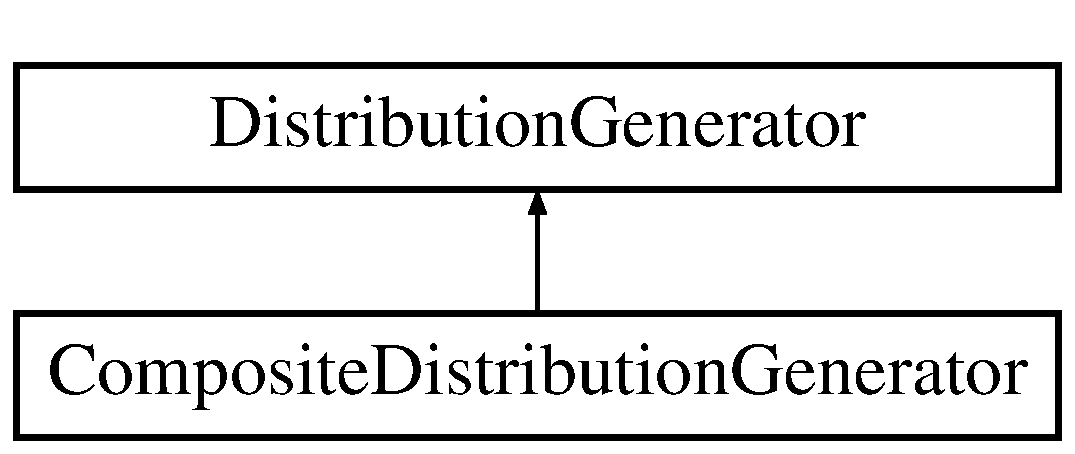
\includegraphics[height=2.000000cm]{d0/df2/class_composite_distribution_generator}
\end{center}
\end{figure}
\subsection*{Public Member Functions}
\begin{DoxyCompactItemize}
\item 
\hyperlink{class_composite_distribution_generator_afdeeb68400f21cb63d4f8fe194ed7e7f}{Composite\+Distribution\+Generator} (vector$<$ \hyperlink{class_distribution_generator}{Distribution\+Generator} $\ast$ $>$ \hyperlink{class_composite_distribution_generator_a9f89632c997c30324e4652ea8bc6d761}{distributions})
\item 
virtual \hyperlink{class_composite_distribution_generator_afdb870d99c1a6fee740abdcc9f4e1c8e}{$\sim$\+Composite\+Distribution\+Generator} ()
\item 
virtual void \hyperlink{class_composite_distribution_generator_a799c7a57b895245c81a9492ddff63384}{initialize} (int seed, double $\ast$\hyperlink{class_distribution_generator_abbb670b1d48a4820559097b85bf6ee2d}{bounding\+Box})
\item 
vector$<$ \hyperlink{structpoint}{point} $>$ \hyperlink{class_composite_distribution_generator_ac5aaadd082a0df0bda42cc8768ecc8d2}{get\+N\+Points} (int n)
\end{DoxyCompactItemize}
\subsection*{Private Attributes}
\begin{DoxyCompactItemize}
\item 
vector$<$ \hyperlink{class_distribution_generator}{Distribution\+Generator} $\ast$ $>$ \hyperlink{class_composite_distribution_generator_a9f89632c997c30324e4652ea8bc6d761}{distributions}
\end{DoxyCompactItemize}
\subsection*{Additional Inherited Members}


\subsection{Detailed Description}
Generate points as the union of several generators. 

\subsection{Constructor \& Destructor Documentation}
\index{Composite\+Distribution\+Generator@{Composite\+Distribution\+Generator}!Composite\+Distribution\+Generator@{Composite\+Distribution\+Generator}}
\index{Composite\+Distribution\+Generator@{Composite\+Distribution\+Generator}!Composite\+Distribution\+Generator@{Composite\+Distribution\+Generator}}
\subsubsection[{\texorpdfstring{Composite\+Distribution\+Generator(vector$<$ Distribution\+Generator $\ast$ $>$ distributions)}{CompositeDistributionGenerator(vector< DistributionGenerator * > distributions)}}]{\setlength{\rightskip}{0pt plus 5cm}Composite\+Distribution\+Generator\+::\+Composite\+Distribution\+Generator (
\begin{DoxyParamCaption}
\item[{vector$<$ {\bf Distribution\+Generator} $\ast$ $>$}]{distributions}
\end{DoxyParamCaption}
)}\hypertarget{class_composite_distribution_generator_afdeeb68400f21cb63d4f8fe194ed7e7f}{}\label{class_composite_distribution_generator_afdeeb68400f21cb63d4f8fe194ed7e7f}
Constructor. 
\begin{DoxyParams}{Parameters}
{\em distributions} & \\
\hline
\end{DoxyParams}
\index{Composite\+Distribution\+Generator@{Composite\+Distribution\+Generator}!````~Composite\+Distribution\+Generator@{$\sim$\+Composite\+Distribution\+Generator}}
\index{````~Composite\+Distribution\+Generator@{$\sim$\+Composite\+Distribution\+Generator}!Composite\+Distribution\+Generator@{Composite\+Distribution\+Generator}}
\subsubsection[{\texorpdfstring{$\sim$\+Composite\+Distribution\+Generator()}{~CompositeDistributionGenerator()}}]{\setlength{\rightskip}{0pt plus 5cm}Composite\+Distribution\+Generator\+::$\sim$\+Composite\+Distribution\+Generator (
\begin{DoxyParamCaption}
{}
\end{DoxyParamCaption}
)\hspace{0.3cm}{\ttfamily [virtual]}}\hypertarget{class_composite_distribution_generator_afdb870d99c1a6fee740abdcc9f4e1c8e}{}\label{class_composite_distribution_generator_afdb870d99c1a6fee740abdcc9f4e1c8e}
Destructor. 

\subsection{Member Function Documentation}
\index{Composite\+Distribution\+Generator@{Composite\+Distribution\+Generator}!get\+N\+Points@{get\+N\+Points}}
\index{get\+N\+Points@{get\+N\+Points}!Composite\+Distribution\+Generator@{Composite\+Distribution\+Generator}}
\subsubsection[{\texorpdfstring{get\+N\+Points(int n)}{getNPoints(int n)}}]{\setlength{\rightskip}{0pt plus 5cm}vector$<$ {\bf point} $>$ Composite\+Distribution\+Generator\+::get\+N\+Points (
\begin{DoxyParamCaption}
\item[{int}]{n}
\end{DoxyParamCaption}
)\hspace{0.3cm}{\ttfamily [virtual]}}\hypertarget{class_composite_distribution_generator_ac5aaadd082a0df0bda42cc8768ecc8d2}{}\label{class_composite_distribution_generator_ac5aaadd082a0df0bda42cc8768ecc8d2}
Return a vector of {\ttfamily n} points of the distribution. 
\begin{DoxyParams}{Parameters}
{\em n} & Amount of output points. \\
\hline
\end{DoxyParams}
\begin{DoxyReturn}{Returns}
Vector of distribution points. 
\end{DoxyReturn}


Implements \hyperlink{class_distribution_generator_a777dcdfd3dee93cfcbcc00969f42ca29}{Distribution\+Generator}.

\index{Composite\+Distribution\+Generator@{Composite\+Distribution\+Generator}!initialize@{initialize}}
\index{initialize@{initialize}!Composite\+Distribution\+Generator@{Composite\+Distribution\+Generator}}
\subsubsection[{\texorpdfstring{initialize(int seed, double $\ast$bounding\+Box)}{initialize(int seed, double *boundingBox)}}]{\setlength{\rightskip}{0pt plus 5cm}void Composite\+Distribution\+Generator\+::initialize (
\begin{DoxyParamCaption}
\item[{int}]{seed, }
\item[{double $\ast$}]{bounding\+Box}
\end{DoxyParamCaption}
)\hspace{0.3cm}{\ttfamily [virtual]}}\hypertarget{class_composite_distribution_generator_a799c7a57b895245c81a9492ddff63384}{}\label{class_composite_distribution_generator_a799c7a57b895245c81a9492ddff63384}
Initializer of the generator. Execute it before any getter call is performed. 

Reimplemented from \hyperlink{class_distribution_generator_ae4fa2d599942539e4b1971b0a8d5f8ba}{Distribution\+Generator}.



\subsection{Member Data Documentation}
\index{Composite\+Distribution\+Generator@{Composite\+Distribution\+Generator}!distributions@{distributions}}
\index{distributions@{distributions}!Composite\+Distribution\+Generator@{Composite\+Distribution\+Generator}}
\subsubsection[{\texorpdfstring{distributions}{distributions}}]{\setlength{\rightskip}{0pt plus 5cm}vector$<${\bf Distribution\+Generator} $\ast$$>$ Composite\+Distribution\+Generator\+::distributions\hspace{0.3cm}{\ttfamily [private]}}\hypertarget{class_composite_distribution_generator_a9f89632c997c30324e4652ea8bc6d761}{}\label{class_composite_distribution_generator_a9f89632c997c30324e4652ea8bc6d761}
Generators 

The documentation for this class was generated from the following files\+:\begin{DoxyCompactItemize}
\item 
structures/domain/Composite\+Distribution\+Generator.\+h\item 
structures/domain/Composite\+Distribution\+Generator.\+cpp\end{DoxyCompactItemize}

\hypertarget{class_constant_constraint_function}{}\section{Constant\+Constraint\+Function$<$ T, S $>$ Class Template Reference}
\label{class_constant_constraint_function}\index{Constant\+Constraint\+Function$<$ T, S $>$@{Constant\+Constraint\+Function$<$ T, S $>$}}
Inheritance diagram for Constant\+Constraint\+Function$<$ T, S $>$\+:\begin{figure}[H]
\begin{center}
\leavevmode
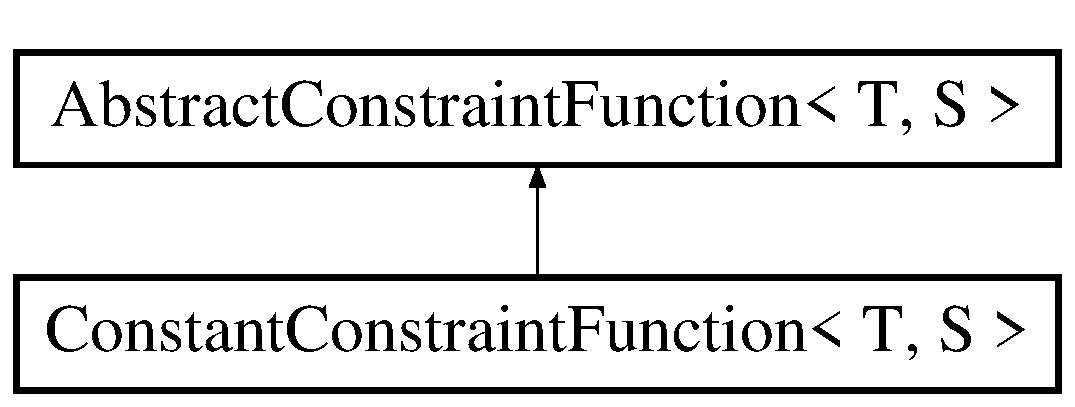
\includegraphics[height=2.000000cm]{d6/d3a/class_constant_constraint_function}
\end{center}
\end{figure}
\subsection*{Public Member Functions}
\begin{DoxyCompactItemize}
\item 
{\bfseries Constant\+Constraint\+Function} (T \hyperlink{class_constant_constraint_function_a9f5066596e6c190c36e7cd9cae09f235}{value})\hypertarget{class_constant_constraint_function_a11f6dcfea30a0d7658fcfb3b2e0d8799}{}\label{class_constant_constraint_function_a11f6dcfea30a0d7658fcfb3b2e0d8799}

\item 
T {\bfseries get\+Value} (S tree\+Condition)\hypertarget{class_constant_constraint_function_a5c6d270fb9c853586247b154d52469cc}{}\label{class_constant_constraint_function_a5c6d270fb9c853586247b154d52469cc}

\end{DoxyCompactItemize}
\subsection*{Private Attributes}
\begin{DoxyCompactItemize}
\item 
T \hyperlink{class_constant_constraint_function_a9f5066596e6c190c36e7cd9cae09f235}{value}
\end{DoxyCompactItemize}


\subsection{Member Data Documentation}
\index{Constant\+Constraint\+Function@{Constant\+Constraint\+Function}!value@{value}}
\index{value@{value}!Constant\+Constraint\+Function@{Constant\+Constraint\+Function}}
\subsubsection[{\texorpdfstring{value}{value}}]{\setlength{\rightskip}{0pt plus 5cm}template$<$class T , class S $>$ T {\bf Constant\+Constraint\+Function}$<$ T, S $>$\+::value\hspace{0.3cm}{\ttfamily [private]}}\hypertarget{class_constant_constraint_function_a9f5066596e6c190c36e7cd9cae09f235}{}\label{class_constant_constraint_function_a9f5066596e6c190c36e7cd9cae09f235}
Constant value. 

The documentation for this class was generated from the following file\+:\begin{DoxyCompactItemize}
\item 
constrains/Constant\+Constraint\+Function.\+h\end{DoxyCompactItemize}

\hypertarget{class_constant_piecewise_constraint_function}{}\section{Constant\+Piecewise\+Constraint\+Function$<$ T, S $>$ Class Template Reference}
\label{class_constant_piecewise_constraint_function}\index{Constant\+Piecewise\+Constraint\+Function$<$ T, S $>$@{Constant\+Piecewise\+Constraint\+Function$<$ T, S $>$}}


{\ttfamily \#include $<$Constant\+Piecewise\+Constraint\+Function.\+h$>$}

Inheritance diagram for Constant\+Piecewise\+Constraint\+Function$<$ T, S $>$\+:\begin{figure}[H]
\begin{center}
\leavevmode
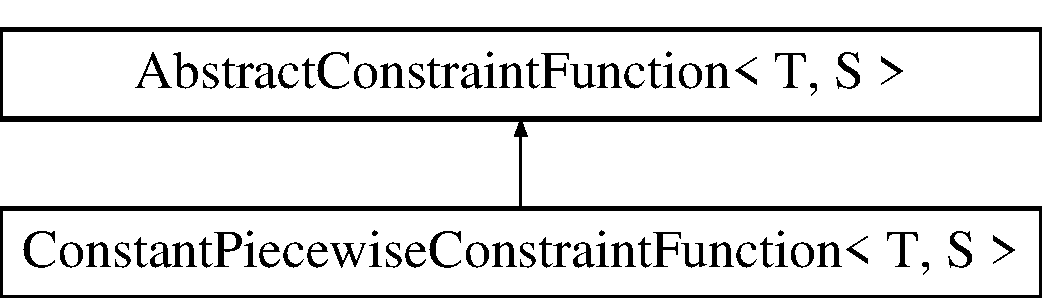
\includegraphics[height=2.000000cm]{d4/d89/class_constant_piecewise_constraint_function}
\end{center}
\end{figure}
\subsection*{Public Member Functions}
\begin{DoxyCompactItemize}
\item 
\hyperlink{class_constant_piecewise_constraint_function_a5f8ebd7b7b8794976f4ddf3a448cd9a6}{Constant\+Piecewise\+Constraint\+Function} (vector$<$ T $>$ \hyperlink{class_constant_piecewise_constraint_function_ae26530a2cd1a3ce9150b68fb16d5423e}{values}, vector$<$ S $>$ \hyperlink{class_constant_piecewise_constraint_function_af28fe38d8c5c4a9a805c8a46d35cd4b2}{conditions})
\item 
virtual \hyperlink{class_constant_piecewise_constraint_function_ab44f248af12827ce5cf528ccf163c2f7}{$\sim$\+Constant\+Piecewise\+Constraint\+Function} ()
\item 
T \hyperlink{class_constant_piecewise_constraint_function_ae44b78e86336e8a45ebac2344d5de8ce}{get\+Value} (S tree\+Condition)
\end{DoxyCompactItemize}
\subsection*{Private Attributes}
\begin{DoxyCompactItemize}
\item 
vector$<$ T $>$ \hyperlink{class_constant_piecewise_constraint_function_ae26530a2cd1a3ce9150b68fb16d5423e}{values}
\item 
vector$<$ S $>$ \hyperlink{class_constant_piecewise_constraint_function_af28fe38d8c5c4a9a805c8a46d35cd4b2}{conditions}
\end{DoxyCompactItemize}


\subsection{Detailed Description}
\subsubsection*{template$<$class T, class S$>$\\*
class Constant\+Piecewise\+Constraint\+Function$<$ T, S $>$}

Constraint piecewise function with different constant values for each condition. 

\subsection{Constructor \& Destructor Documentation}
\index{Constant\+Piecewise\+Constraint\+Function@{Constant\+Piecewise\+Constraint\+Function}!Constant\+Piecewise\+Constraint\+Function@{Constant\+Piecewise\+Constraint\+Function}}
\index{Constant\+Piecewise\+Constraint\+Function@{Constant\+Piecewise\+Constraint\+Function}!Constant\+Piecewise\+Constraint\+Function@{Constant\+Piecewise\+Constraint\+Function}}
\subsubsection[{\texorpdfstring{Constant\+Piecewise\+Constraint\+Function(vector$<$ T $>$ values, vector$<$ S $>$ conditions)}{ConstantPiecewiseConstraintFunction(vector< T > values, vector< S > conditions)}}]{\setlength{\rightskip}{0pt plus 5cm}template$<$class T , class S $>$ {\bf Constant\+Piecewise\+Constraint\+Function}$<$ T, S $>$\+::{\bf Constant\+Piecewise\+Constraint\+Function} (
\begin{DoxyParamCaption}
\item[{vector$<$ T $>$}]{values, }
\item[{vector$<$ S $>$}]{conditions}
\end{DoxyParamCaption}
)}\hypertarget{class_constant_piecewise_constraint_function_a5f8ebd7b7b8794976f4ddf3a448cd9a6}{}\label{class_constant_piecewise_constraint_function_a5f8ebd7b7b8794976f4ddf3a448cd9a6}
Constructor. 
\begin{DoxyParams}{Parameters}
{\em values} & Piecewise constant values for each function piece. \\
\hline
{\em conditions} & Lower bound condition for each function piece. \\
\hline
\end{DoxyParams}
\index{Constant\+Piecewise\+Constraint\+Function@{Constant\+Piecewise\+Constraint\+Function}!````~Constant\+Piecewise\+Constraint\+Function@{$\sim$\+Constant\+Piecewise\+Constraint\+Function}}
\index{````~Constant\+Piecewise\+Constraint\+Function@{$\sim$\+Constant\+Piecewise\+Constraint\+Function}!Constant\+Piecewise\+Constraint\+Function@{Constant\+Piecewise\+Constraint\+Function}}
\subsubsection[{\texorpdfstring{$\sim$\+Constant\+Piecewise\+Constraint\+Function()}{~ConstantPiecewiseConstraintFunction()}}]{\setlength{\rightskip}{0pt plus 5cm}template$<$class T , class S $>$ {\bf Constant\+Piecewise\+Constraint\+Function}$<$ T, S $>$\+::$\sim${\bf Constant\+Piecewise\+Constraint\+Function} (
\begin{DoxyParamCaption}
{}
\end{DoxyParamCaption}
)\hspace{0.3cm}{\ttfamily [virtual]}}\hypertarget{class_constant_piecewise_constraint_function_ab44f248af12827ce5cf528ccf163c2f7}{}\label{class_constant_piecewise_constraint_function_ab44f248af12827ce5cf528ccf163c2f7}
Destructor. 

\subsection{Member Function Documentation}
\index{Constant\+Piecewise\+Constraint\+Function@{Constant\+Piecewise\+Constraint\+Function}!get\+Value@{get\+Value}}
\index{get\+Value@{get\+Value}!Constant\+Piecewise\+Constraint\+Function@{Constant\+Piecewise\+Constraint\+Function}}
\subsubsection[{\texorpdfstring{get\+Value(\+S tree\+Condition)}{getValue(S treeCondition)}}]{\setlength{\rightskip}{0pt plus 5cm}template$<$class T , class S $>$ T {\bf Constant\+Piecewise\+Constraint\+Function}$<$ T, S $>$\+::get\+Value (
\begin{DoxyParamCaption}
\item[{S}]{tree\+Condition}
\end{DoxyParamCaption}
)\hspace{0.3cm}{\ttfamily [virtual]}}\hypertarget{class_constant_piecewise_constraint_function_ae44b78e86336e8a45ebac2344d5de8ce}{}\label{class_constant_piecewise_constraint_function_ae44b78e86336e8a45ebac2344d5de8ce}
Estimator based on the condition {\ttfamily tree\+Condition}. 
\begin{DoxyParams}{Parameters}
{\em tree\+Condition} & Condition value. \\
\hline
\end{DoxyParams}
\begin{DoxyReturn}{Returns}
Constraint function value. 
\end{DoxyReturn}


Implements \hyperlink{class_abstract_constraint_function}{Abstract\+Constraint\+Function$<$ T, S $>$}.



\subsection{Member Data Documentation}
\index{Constant\+Piecewise\+Constraint\+Function@{Constant\+Piecewise\+Constraint\+Function}!conditions@{conditions}}
\index{conditions@{conditions}!Constant\+Piecewise\+Constraint\+Function@{Constant\+Piecewise\+Constraint\+Function}}
\subsubsection[{\texorpdfstring{conditions}{conditions}}]{\setlength{\rightskip}{0pt plus 5cm}template$<$class T , class S $>$ vector$<$S$>$ {\bf Constant\+Piecewise\+Constraint\+Function}$<$ T, S $>$\+::conditions\hspace{0.3cm}{\ttfamily [private]}}\hypertarget{class_constant_piecewise_constraint_function_af28fe38d8c5c4a9a805c8a46d35cd4b2}{}\label{class_constant_piecewise_constraint_function_af28fe38d8c5c4a9a805c8a46d35cd4b2}
Lower bound condition for each function piece. The upper bounds are the next lower bound. S must define the operator $>$=. \index{Constant\+Piecewise\+Constraint\+Function@{Constant\+Piecewise\+Constraint\+Function}!values@{values}}
\index{values@{values}!Constant\+Piecewise\+Constraint\+Function@{Constant\+Piecewise\+Constraint\+Function}}
\subsubsection[{\texorpdfstring{values}{values}}]{\setlength{\rightskip}{0pt plus 5cm}template$<$class T , class S $>$ vector$<$T$>$ {\bf Constant\+Piecewise\+Constraint\+Function}$<$ T, S $>$\+::values\hspace{0.3cm}{\ttfamily [private]}}\hypertarget{class_constant_piecewise_constraint_function_ae26530a2cd1a3ce9150b68fb16d5423e}{}\label{class_constant_piecewise_constraint_function_ae26530a2cd1a3ce9150b68fb16d5423e}
Piecewise constant values for each function piece. 

The documentation for this class was generated from the following file\+:\begin{DoxyCompactItemize}
\item 
constrains/Constant\+Piecewise\+Constraint\+Function.\+h\end{DoxyCompactItemize}

\hypertarget{class_cylinder_creator}{}\section{Cylinder\+Creator Class Reference}
\label{class_cylinder_creator}\index{Cylinder\+Creator@{Cylinder\+Creator}}


{\ttfamily \#include $<$Cylinder\+Creator.\+h$>$}

Inheritance diagram for Cylinder\+Creator\+:\begin{figure}[H]
\begin{center}
\leavevmode
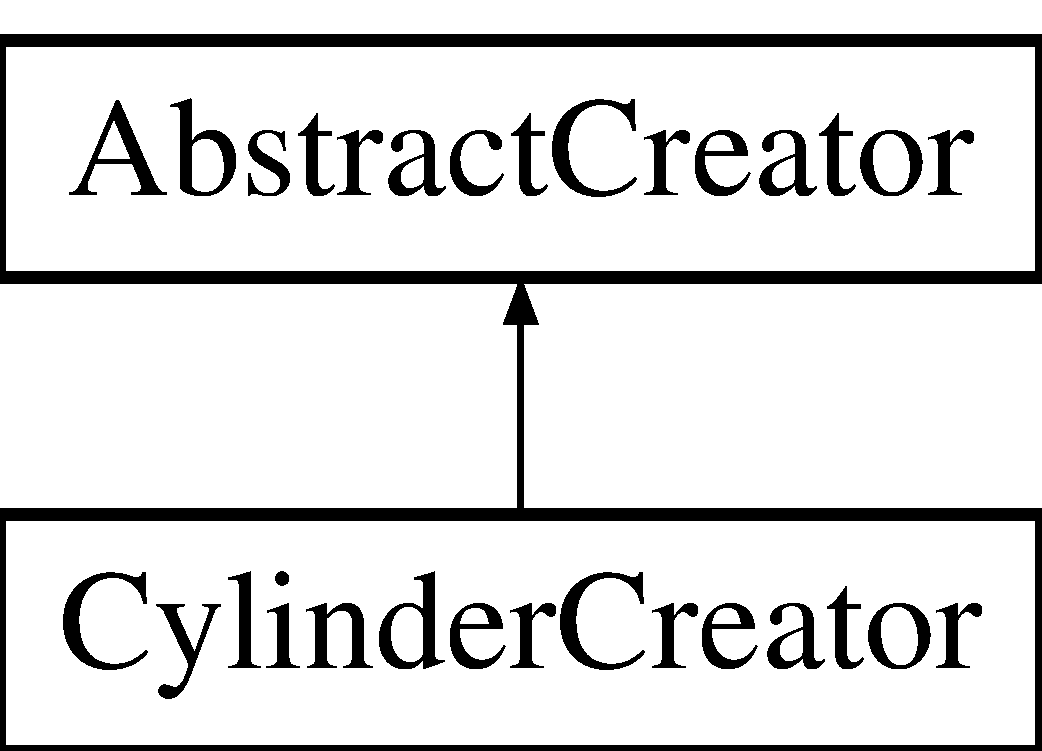
\includegraphics[height=2.000000cm]{d0/d29/class_cylinder_creator}
\end{center}
\end{figure}
\subsection*{Public Member Functions}
\begin{DoxyCompactItemize}
\item 
\hyperlink{class_cylinder_creator_a3bd3c0c293bbc17c02cc5512c96695c5}{Cylinder\+Creator} (vector$<$ double $>$ \hyperlink{class_cylinder_creator_a78f2d1a2db1e3915e182fc102ad4ac96}{center}, double \hyperlink{class_cylinder_creator_a3558e3005e9567532b04a8f1d32ff4a4}{radius}, double \hyperlink{class_cylinder_creator_acd2b5826bf983377bb0f013c01e7329f}{height}, int \hyperlink{class_cylinder_creator_a9bb62db1072cadf1cce2962c7b954b9b}{resolution})
\item 
virtual \hyperlink{class_cylinder_creator_aa7b5874b41e919104682ca0e925f897a}{$\sim$\+Cylinder\+Creator} ()
\item 
void \hyperlink{class_cylinder_creator_ae4da1cf60c40253ab7f677d8d708eefe}{create} (string filename)
\end{DoxyCompactItemize}
\subsection*{Private Attributes}
\begin{DoxyCompactItemize}
\item 
vector$<$ double $>$ \hyperlink{class_cylinder_creator_a78f2d1a2db1e3915e182fc102ad4ac96}{center}
\item 
double \hyperlink{class_cylinder_creator_a3558e3005e9567532b04a8f1d32ff4a4}{radius}
\item 
double \hyperlink{class_cylinder_creator_acd2b5826bf983377bb0f013c01e7329f}{height}
\item 
int \hyperlink{class_cylinder_creator_a9bb62db1072cadf1cce2962c7b954b9b}{resolution}
\end{DoxyCompactItemize}


\subsection{Detailed Description}
Creates a V\+TP file containing a cylinder. 

\subsection{Constructor \& Destructor Documentation}
\index{Cylinder\+Creator@{Cylinder\+Creator}!Cylinder\+Creator@{Cylinder\+Creator}}
\index{Cylinder\+Creator@{Cylinder\+Creator}!Cylinder\+Creator@{Cylinder\+Creator}}
\subsubsection[{\texorpdfstring{Cylinder\+Creator(vector$<$ double $>$ center, double radius, double height, int resolution)}{CylinderCreator(vector< double > center, double radius, double height, int resolution)}}]{\setlength{\rightskip}{0pt plus 5cm}Cylinder\+Creator\+::\+Cylinder\+Creator (
\begin{DoxyParamCaption}
\item[{vector$<$ double $>$}]{center, }
\item[{double}]{radius, }
\item[{double}]{height, }
\item[{int}]{resolution}
\end{DoxyParamCaption}
)}\hypertarget{class_cylinder_creator_a3bd3c0c293bbc17c02cc5512c96695c5}{}\label{class_cylinder_creator_a3bd3c0c293bbc17c02cc5512c96695c5}
Initialize the inner variables of the object. 
\begin{DoxyParams}{Parameters}
{\em center} & 3D point denoting the center of the sphere. \\
\hline
{\em radius} & Radius of the cylinder base. \\
\hline
{\em height} & Height of the cylinder. \\
\hline
{\em resolution} & Circumferential resolution. \\
\hline
\end{DoxyParams}
\index{Cylinder\+Creator@{Cylinder\+Creator}!````~Cylinder\+Creator@{$\sim$\+Cylinder\+Creator}}
\index{````~Cylinder\+Creator@{$\sim$\+Cylinder\+Creator}!Cylinder\+Creator@{Cylinder\+Creator}}
\subsubsection[{\texorpdfstring{$\sim$\+Cylinder\+Creator()}{~CylinderCreator()}}]{\setlength{\rightskip}{0pt plus 5cm}Cylinder\+Creator\+::$\sim$\+Cylinder\+Creator (
\begin{DoxyParamCaption}
{}
\end{DoxyParamCaption}
)\hspace{0.3cm}{\ttfamily [virtual]}}\hypertarget{class_cylinder_creator_aa7b5874b41e919104682ca0e925f897a}{}\label{class_cylinder_creator_aa7b5874b41e919104682ca0e925f897a}
Standard destructor. 

\subsection{Member Function Documentation}
\index{Cylinder\+Creator@{Cylinder\+Creator}!create@{create}}
\index{create@{create}!Cylinder\+Creator@{Cylinder\+Creator}}
\subsubsection[{\texorpdfstring{create(string filename)}{create(string filename)}}]{\setlength{\rightskip}{0pt plus 5cm}void Cylinder\+Creator\+::create (
\begin{DoxyParamCaption}
\item[{string}]{filename}
\end{DoxyParamCaption}
)\hspace{0.3cm}{\ttfamily [virtual]}}\hypertarget{class_cylinder_creator_ae4da1cf60c40253ab7f677d8d708eefe}{}\label{class_cylinder_creator_ae4da1cf60c40253ab7f677d8d708eefe}
Persist the object in a file with V\+TP format. 
\begin{DoxyParams}{Parameters}
{\em filename} & Save file for the current object. \\
\hline
\end{DoxyParams}


Implements \hyperlink{class_abstract_creator_a1991e446444ffea2b85216b64f2dcf9e}{Abstract\+Creator}.



\subsection{Member Data Documentation}
\index{Cylinder\+Creator@{Cylinder\+Creator}!center@{center}}
\index{center@{center}!Cylinder\+Creator@{Cylinder\+Creator}}
\subsubsection[{\texorpdfstring{center}{center}}]{\setlength{\rightskip}{0pt plus 5cm}vector$<$double$>$ Cylinder\+Creator\+::center\hspace{0.3cm}{\ttfamily [private]}}\hypertarget{class_cylinder_creator_a78f2d1a2db1e3915e182fc102ad4ac96}{}\label{class_cylinder_creator_a78f2d1a2db1e3915e182fc102ad4ac96}
3D point denoting the center of the sphere. \index{Cylinder\+Creator@{Cylinder\+Creator}!height@{height}}
\index{height@{height}!Cylinder\+Creator@{Cylinder\+Creator}}
\subsubsection[{\texorpdfstring{height}{height}}]{\setlength{\rightskip}{0pt plus 5cm}double Cylinder\+Creator\+::height\hspace{0.3cm}{\ttfamily [private]}}\hypertarget{class_cylinder_creator_acd2b5826bf983377bb0f013c01e7329f}{}\label{class_cylinder_creator_acd2b5826bf983377bb0f013c01e7329f}
Height of the cylinder. \index{Cylinder\+Creator@{Cylinder\+Creator}!radius@{radius}}
\index{radius@{radius}!Cylinder\+Creator@{Cylinder\+Creator}}
\subsubsection[{\texorpdfstring{radius}{radius}}]{\setlength{\rightskip}{0pt plus 5cm}double Cylinder\+Creator\+::radius\hspace{0.3cm}{\ttfamily [private]}}\hypertarget{class_cylinder_creator_a3558e3005e9567532b04a8f1d32ff4a4}{}\label{class_cylinder_creator_a3558e3005e9567532b04a8f1d32ff4a4}
Radius of the cylinder base. \index{Cylinder\+Creator@{Cylinder\+Creator}!resolution@{resolution}}
\index{resolution@{resolution}!Cylinder\+Creator@{Cylinder\+Creator}}
\subsubsection[{\texorpdfstring{resolution}{resolution}}]{\setlength{\rightskip}{0pt plus 5cm}int Cylinder\+Creator\+::resolution\hspace{0.3cm}{\ttfamily [private]}}\hypertarget{class_cylinder_creator_a9bb62db1072cadf1cce2962c7b954b9b}{}\label{class_cylinder_creator_a9bb62db1072cadf1cce2962c7b954b9b}
Circumferential resolution. 

The documentation for this class was generated from the following files\+:\begin{DoxyCompactItemize}
\item 
creators/Cylinder\+Creator.\+h\item 
creators/Cylinder\+Creator.\+cpp\end{DoxyCompactItemize}

\hypertarget{class_distribution_generator}{}\section{Distribution\+Generator Class Reference}
\label{class_distribution_generator}\index{Distribution\+Generator@{Distribution\+Generator}}


{\ttfamily \#include $<$Distribution\+Generator.\+h$>$}

Inheritance diagram for Distribution\+Generator\+:\begin{figure}[H]
\begin{center}
\leavevmode
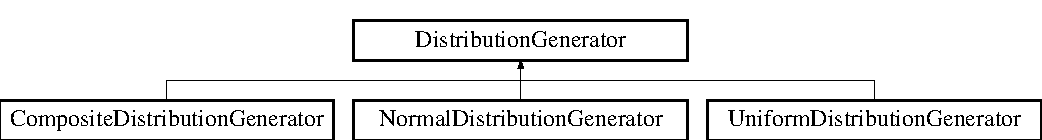
\includegraphics[height=2.000000cm]{dc/dc8/class_distribution_generator}
\end{center}
\end{figure}
\subsection*{Public Member Functions}
\begin{DoxyCompactItemize}
\item 
\hyperlink{class_distribution_generator_a9ade678342c897fddf74da6a453cfa7b}{Distribution\+Generator} ()
\item 
virtual \hyperlink{class_distribution_generator_ada1c1b4e9024716e3041ee7836deff65}{$\sim$\+Distribution\+Generator} ()
\item 
virtual void \hyperlink{class_distribution_generator_ae4fa2d599942539e4b1971b0a8d5f8ba}{initialize} (int seed, double $\ast$\hyperlink{class_distribution_generator_abbb670b1d48a4820559097b85bf6ee2d}{bounding\+Box})
\item 
virtual vector$<$ \hyperlink{structpoint}{point} $>$ \hyperlink{class_distribution_generator_a777dcdfd3dee93cfcbcc00969f42ca29}{get\+N\+Points} (int n)=0
\end{DoxyCompactItemize}
\subsection*{Protected Attributes}
\begin{DoxyCompactItemize}
\item 
double $\ast$ \hyperlink{class_distribution_generator_abbb670b1d48a4820559097b85bf6ee2d}{bounding\+Box}
\item 
mt19937 \hyperlink{class_distribution_generator_a875697de8d5c0a4d18e473e483a9646c}{generator}
\end{DoxyCompactItemize}


\subsection{Detailed Description}
Abstract generator of points. 

\subsection{Constructor \& Destructor Documentation}
\index{Distribution\+Generator@{Distribution\+Generator}!Distribution\+Generator@{Distribution\+Generator}}
\index{Distribution\+Generator@{Distribution\+Generator}!Distribution\+Generator@{Distribution\+Generator}}
\subsubsection[{\texorpdfstring{Distribution\+Generator()}{DistributionGenerator()}}]{\setlength{\rightskip}{0pt plus 5cm}Distribution\+Generator\+::\+Distribution\+Generator (
\begin{DoxyParamCaption}
{}
\end{DoxyParamCaption}
)}\hypertarget{class_distribution_generator_a9ade678342c897fddf74da6a453cfa7b}{}\label{class_distribution_generator_a9ade678342c897fddf74da6a453cfa7b}
Constructor \index{Distribution\+Generator@{Distribution\+Generator}!````~Distribution\+Generator@{$\sim$\+Distribution\+Generator}}
\index{````~Distribution\+Generator@{$\sim$\+Distribution\+Generator}!Distribution\+Generator@{Distribution\+Generator}}
\subsubsection[{\texorpdfstring{$\sim$\+Distribution\+Generator()}{~DistributionGenerator()}}]{\setlength{\rightskip}{0pt plus 5cm}Distribution\+Generator\+::$\sim$\+Distribution\+Generator (
\begin{DoxyParamCaption}
{}
\end{DoxyParamCaption}
)\hspace{0.3cm}{\ttfamily [virtual]}}\hypertarget{class_distribution_generator_ada1c1b4e9024716e3041ee7836deff65}{}\label{class_distribution_generator_ada1c1b4e9024716e3041ee7836deff65}
Destructor 

\subsection{Member Function Documentation}
\index{Distribution\+Generator@{Distribution\+Generator}!get\+N\+Points@{get\+N\+Points}}
\index{get\+N\+Points@{get\+N\+Points}!Distribution\+Generator@{Distribution\+Generator}}
\subsubsection[{\texorpdfstring{get\+N\+Points(int n)=0}{getNPoints(int n)=0}}]{\setlength{\rightskip}{0pt plus 5cm}virtual vector$<${\bf point}$>$ Distribution\+Generator\+::get\+N\+Points (
\begin{DoxyParamCaption}
\item[{int}]{n}
\end{DoxyParamCaption}
)\hspace{0.3cm}{\ttfamily [pure virtual]}}\hypertarget{class_distribution_generator_a777dcdfd3dee93cfcbcc00969f42ca29}{}\label{class_distribution_generator_a777dcdfd3dee93cfcbcc00969f42ca29}
Return a vector of {\ttfamily n} points of the distribution. 
\begin{DoxyParams}{Parameters}
{\em n} & Amount of output points. \\
\hline
\end{DoxyParams}
\begin{DoxyReturn}{Returns}
Vector of distribution points. 
\end{DoxyReturn}


Implemented in \hyperlink{class_uniform_distribution_generator_a3628de975c16748b69b5838e4b02ea41}{Uniform\+Distribution\+Generator}.

\index{Distribution\+Generator@{Distribution\+Generator}!initialize@{initialize}}
\index{initialize@{initialize}!Distribution\+Generator@{Distribution\+Generator}}
\subsubsection[{\texorpdfstring{initialize(int seed, double $\ast$bounding\+Box)}{initialize(int seed, double *boundingBox)}}]{\setlength{\rightskip}{0pt plus 5cm}void Distribution\+Generator\+::initialize (
\begin{DoxyParamCaption}
\item[{int}]{seed, }
\item[{double $\ast$}]{bounding\+Box}
\end{DoxyParamCaption}
)\hspace{0.3cm}{\ttfamily [virtual]}}\hypertarget{class_distribution_generator_ae4fa2d599942539e4b1971b0a8d5f8ba}{}\label{class_distribution_generator_ae4fa2d599942539e4b1971b0a8d5f8ba}
Initializer of the generator. Execute it before any getter call is performed. 

Reimplemented in \hyperlink{class_uniform_distribution_generator_a9f40ba5dca7db03833f00a846218ae68}{Uniform\+Distribution\+Generator}.



\subsection{Member Data Documentation}
\index{Distribution\+Generator@{Distribution\+Generator}!bounding\+Box@{bounding\+Box}}
\index{bounding\+Box@{bounding\+Box}!Distribution\+Generator@{Distribution\+Generator}}
\subsubsection[{\texorpdfstring{bounding\+Box}{boundingBox}}]{\setlength{\rightskip}{0pt plus 5cm}double$\ast$ Distribution\+Generator\+::bounding\+Box\hspace{0.3cm}{\ttfamily [protected]}}\hypertarget{class_distribution_generator_abbb670b1d48a4820559097b85bf6ee2d}{}\label{class_distribution_generator_abbb670b1d48a4820559097b85bf6ee2d}
Bounding box of the domain where the points will be generated. \index{Distribution\+Generator@{Distribution\+Generator}!generator@{generator}}
\index{generator@{generator}!Distribution\+Generator@{Distribution\+Generator}}
\subsubsection[{\texorpdfstring{generator}{generator}}]{\setlength{\rightskip}{0pt plus 5cm}mt19937 Distribution\+Generator\+::generator\hspace{0.3cm}{\ttfamily [protected]}}\hypertarget{class_distribution_generator_a875697de8d5c0a4d18e473e483a9646c}{}\label{class_distribution_generator_a875697de8d5c0a4d18e473e483a9646c}
Random generator. 

The documentation for this class was generated from the following files\+:\begin{DoxyCompactItemize}
\item 
structures/domain/Distribution\+Generator.\+h\item 
structures/domain/Distribution\+Generator.\+cpp\end{DoxyCompactItemize}

\hypertarget{class_domain_n_v_r}{}\section{Domain\+N\+VR Class Reference}
\label{class_domain_n_v_r}\index{Domain\+N\+VR@{Domain\+N\+VR}}


{\ttfamily \#include $<$Domain\+N\+V\+R.\+h$>$}

Inheritance diagram for Domain\+N\+VR\+:\begin{figure}[H]
\begin{center}
\leavevmode
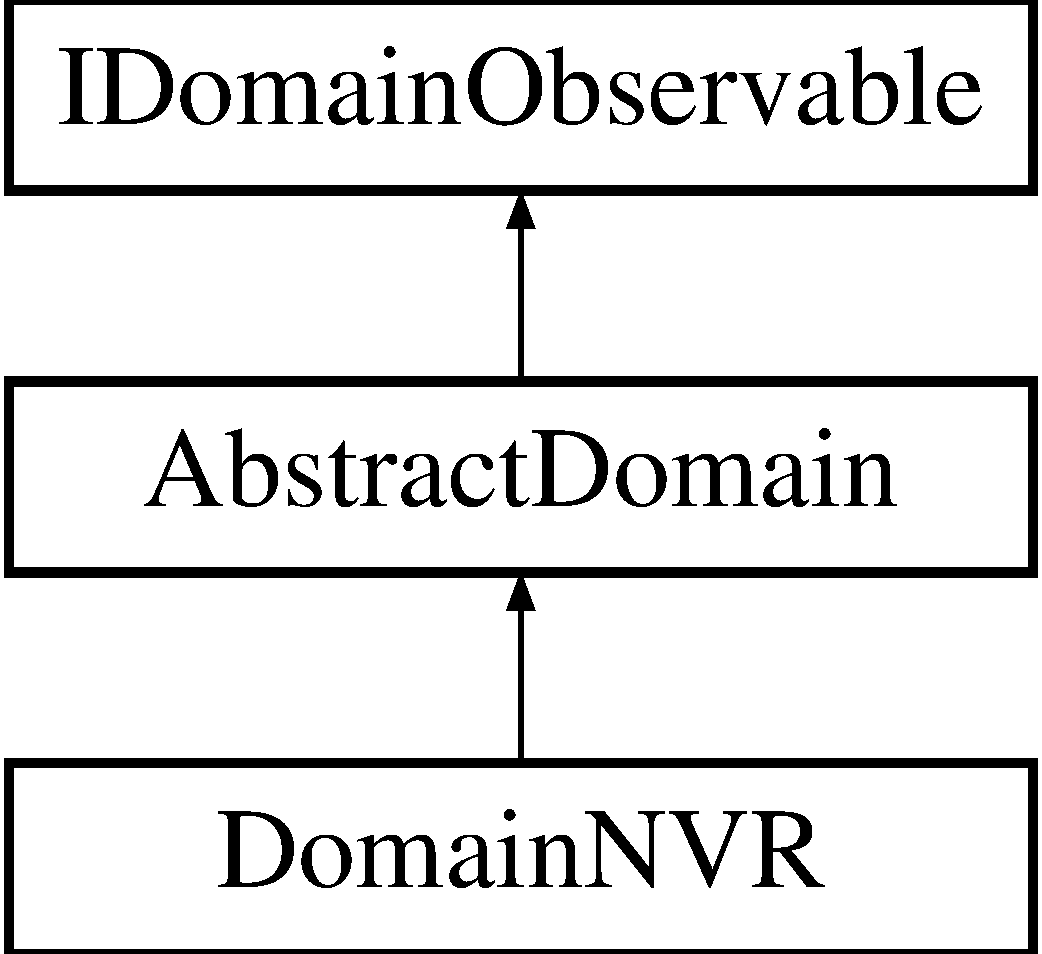
\includegraphics[height=3.000000cm]{d0/d25/class_domain_n_v_r}
\end{center}
\end{figure}
\subsection*{Public Member Functions}
\begin{DoxyCompactItemize}
\item 
\hyperlink{class_domain_n_v_r_a431e9b827836f231d6acc002332eb6a1}{Domain\+N\+VR} (string filename\+Hull, vector$<$ string $>$ filename\+Non\+Vascular\+Regions, \hyperlink{class_generator_data}{Generator\+Data} $\ast$\hyperlink{class_abstract_domain_aa37fbabc2bfa92c574f7db7544016b53}{instance\+Data})
\item 
\hyperlink{class_domain_n_v_r_af24a5b01a05b7e07c7cb0ba401dbb209}{Domain\+N\+VR} (string filename\+Hull, vector$<$ string $>$ filename\+Non\+Vascular\+Regions, int \hyperlink{class_domain_n_v_r_aa8a3d85f1a554c27e0ca399924576822}{n\+Draw}, \hyperlink{class_generator_data}{Generator\+Data} $\ast$\hyperlink{class_abstract_domain_aa37fbabc2bfa92c574f7db7544016b53}{instance\+Data})
\item 
\hyperlink{class_domain_n_v_r_abf32bdc762f1baacd89e14daf3e65bd7}{Domain\+N\+VR} (string filename\+Hull, vector$<$ string $>$ filename\+Non\+Vascular\+Regions, int \hyperlink{class_domain_n_v_r_aa8a3d85f1a554c27e0ca399924576822}{n\+Draw}, int \hyperlink{class_domain_n_v_r_aaf470f5f729cb3fc68d5449c52eccde5}{seed}, \hyperlink{class_generator_data}{Generator\+Data} $\ast$\hyperlink{class_abstract_domain_aa37fbabc2bfa92c574f7db7544016b53}{instance\+Data})
\item 
int \hyperlink{class_domain_n_v_r_a46b7a56ffdb8f8e0cfcd2a5761571394}{is\+Segment\+Inside} (\hyperlink{structpoint}{point} xs, \hyperlink{structpoint}{point} xf)
\item 
double \hyperlink{class_domain_n_v_r_a590ea752ce83767038de90138faf8a21}{get\+Characteristic\+Length} ()
\item 
double \hyperlink{class_domain_n_v_r_a5e67e5367a9f22ab0243e06d92abccab}{get\+D\+Lim} (long long int n\+Vessels, double factor)
\item 
double $\ast$ \hyperlink{class_domain_n_v_r_a5d97b6894250d8034c5e0679266f9fb1}{get\+Local\+Neighborhood} (\hyperlink{structpoint}{point} p, long long int n\+Vessels)
\item 
double \hyperlink{class_domain_n_v_r_aae7b6782c1caab8cf5246c802be410cc}{get\+Size} ()
\item 
virtual \hyperlink{structpoint}{point} \hyperlink{class_domain_n_v_r_a88c76433bc3e8a1c1d60d4e7643f46d0}{get\+Random\+Point} ()
\item 
vtk\+Smart\+Pointer$<$ vtk\+O\+B\+B\+Tree $>$ \& \hyperlink{class_domain_n_v_r_a504fa4fb67064bdf3b1507a1d7372d41}{get\+Locator} ()
\item 
int \hyperlink{class_domain_n_v_r_a3fead46c8720529bc3faaae5b817ccb7}{get\+Draw} ()
\item 
deque$<$ \hyperlink{structpoint}{point} $>$ \& \hyperlink{class_domain_n_v_r_a2b303bccf9a1db72e3bae866d7947f2d}{get\+Random\+Inner\+Points} ()
\item 
vtk\+Smart\+Pointer$<$ vtk\+Poly\+Data $>$ \& \hyperlink{class_domain_n_v_r_a50591c2d4b9e055821cc53416bf4263c}{get\+Vtk\+Geometry} ()
\end{DoxyCompactItemize}
\subsection*{Protected Member Functions}
\begin{DoxyCompactItemize}
\item 
void {\bfseries generate\+Random\+Points} ()\hypertarget{class_domain_n_v_r_a7bcd43488a6810609d6004653d36566f}{}\label{class_domain_n_v_r_a7bcd43488a6810609d6004653d36566f}

\item 
void {\bfseries remove\+Random\+Outer\+Points} ()\hypertarget{class_domain_n_v_r_aae7ebe5baaefe6824097127c8d91bb2c}{}\label{class_domain_n_v_r_aae7ebe5baaefe6824097127c8d91bb2c}

\end{DoxyCompactItemize}
\subsection*{Protected Attributes}
\begin{DoxyCompactItemize}
\item 
deque$<$ \hyperlink{structpoint}{point} $>$ {\bfseries random\+Inner\+Points}\hypertarget{class_domain_n_v_r_a8fbb161c35df4d674c42fcf0baa76284}{}\label{class_domain_n_v_r_a8fbb161c35df4d674c42fcf0baa76284}

\end{DoxyCompactItemize}
\subsection*{Private Attributes}
\begin{DoxyCompactItemize}
\item 
vtk\+Smart\+Pointer$<$ vtk\+Poly\+Data $>$ \hyperlink{class_domain_n_v_r_a4870df18eb5b742c6a76ad9ba04533a2}{vtk\+Geometry}
\item 
vector$<$ vtk\+Smart\+Pointer$<$ vtk\+Poly\+Data $>$ $>$ \hyperlink{class_domain_n_v_r_aff487471a8d4fc7b0a5cfeeb119f8471}{vtk\+Hollow\+Regions}
\item 
vtk\+Smart\+Pointer$<$ vtk\+O\+B\+B\+Tree $>$ \hyperlink{class_domain_n_v_r_a3352f4af5dcc9c78cf2a56fd720da497}{locator}
\item 
vector$<$ vtk\+Smart\+Pointer$<$ vtk\+O\+B\+B\+Tree $>$ $>$ \hyperlink{class_domain_n_v_r_a8848ec8d5e22bb9d03bd946087f0fa00}{hollow\+Locators}
\item 
double \hyperlink{class_domain_n_v_r_a7806401ba6d4de5d8e39d0f468f23ff2}{characteristic\+Length}
\item 
int \hyperlink{class_domain_n_v_r_aa8a3d85f1a554c27e0ca399924576822}{n\+Draw}
\item 
int \hyperlink{class_domain_n_v_r_aaf470f5f729cb3fc68d5449c52eccde5}{seed} = -\/1
\item 
mt19937 \hyperlink{class_domain_n_v_r_a0b5be1fa94ce69a9af453274122b8387}{generator}
\end{DoxyCompactItemize}


\subsection{Detailed Description}
Domain with non-\/vascularized regions. 

\subsection{Constructor \& Destructor Documentation}
\index{Domain\+N\+VR@{Domain\+N\+VR}!Domain\+N\+VR@{Domain\+N\+VR}}
\index{Domain\+N\+VR@{Domain\+N\+VR}!Domain\+N\+VR@{Domain\+N\+VR}}
\subsubsection[{\texorpdfstring{Domain\+N\+V\+R(string filename\+Hull, vector$<$ string $>$ filename\+Non\+Vascular\+Regions, Generator\+Data $\ast$instance\+Data)}{DomainNVR(string filenameHull, vector< string > filenameNonVascularRegions, GeneratorData *instanceData)}}]{\setlength{\rightskip}{0pt plus 5cm}Domain\+N\+V\+R\+::\+Domain\+N\+VR (
\begin{DoxyParamCaption}
\item[{string}]{filename\+Hull, }
\item[{vector$<$ string $>$}]{filename\+Non\+Vascular\+Regions, }
\item[{{\bf Generator\+Data} $\ast$}]{instance\+Data}
\end{DoxyParamCaption}
)}\hypertarget{class_domain_n_v_r_a431e9b827836f231d6acc002332eb6a1}{}\label{class_domain_n_v_r_a431e9b827836f231d6acc002332eb6a1}
Constructs a domain shaped by {\ttfamily filename\+Hull} with non vascularized regions contained in {\ttfamily filename\+Non\+Vascular\+Regions}. 
\begin{DoxyParams}{Parameters}
{\em filename\+Hull} & Domain description. \\
\hline
{\em filename\+Non\+Vascular\+Regions} & Non-\/vascularized regions descriptions. \\
\hline
\end{DoxyParams}
\index{Domain\+N\+VR@{Domain\+N\+VR}!Domain\+N\+VR@{Domain\+N\+VR}}
\index{Domain\+N\+VR@{Domain\+N\+VR}!Domain\+N\+VR@{Domain\+N\+VR}}
\subsubsection[{\texorpdfstring{Domain\+N\+V\+R(string filename\+Hull, vector$<$ string $>$ filename\+Non\+Vascular\+Regions, int n\+Draw, Generator\+Data $\ast$instance\+Data)}{DomainNVR(string filenameHull, vector< string > filenameNonVascularRegions, int nDraw, GeneratorData *instanceData)}}]{\setlength{\rightskip}{0pt plus 5cm}Domain\+N\+V\+R\+::\+Domain\+N\+VR (
\begin{DoxyParamCaption}
\item[{string}]{filename\+Hull, }
\item[{vector$<$ string $>$}]{filename\+Non\+Vascular\+Regions, }
\item[{int}]{n\+Draw, }
\item[{{\bf Generator\+Data} $\ast$}]{instance\+Data}
\end{DoxyParamCaption}
)}\hypertarget{class_domain_n_v_r_af24a5b01a05b7e07c7cb0ba401dbb209}{}\label{class_domain_n_v_r_af24a5b01a05b7e07c7cb0ba401dbb209}
Constructs a domain shaped by {\ttfamily filename\+Hull} with non vascularized regions contained in {\ttfamily filename\+Non\+Vascular\+Regions} which generates batches of {\ttfamily n\+Draw} random points each time that the domain is with no more points. 
\begin{DoxyParams}{Parameters}
{\em filename\+Hull} & Domain description. \\
\hline
{\em filename\+Non\+Vascular\+Regions} & Non-\/vascularized regions descriptions. \\
\hline
{\em n\+Draw} & Random points generated at each batch. \\
\hline
\end{DoxyParams}
\index{Domain\+N\+VR@{Domain\+N\+VR}!Domain\+N\+VR@{Domain\+N\+VR}}
\index{Domain\+N\+VR@{Domain\+N\+VR}!Domain\+N\+VR@{Domain\+N\+VR}}
\subsubsection[{\texorpdfstring{Domain\+N\+V\+R(string filename\+Hull, vector$<$ string $>$ filename\+Non\+Vascular\+Regions, int n\+Draw, int seed, Generator\+Data $\ast$instance\+Data)}{DomainNVR(string filenameHull, vector< string > filenameNonVascularRegions, int nDraw, int seed, GeneratorData *instanceData)}}]{\setlength{\rightskip}{0pt plus 5cm}Domain\+N\+V\+R\+::\+Domain\+N\+VR (
\begin{DoxyParamCaption}
\item[{string}]{filename\+Hull, }
\item[{vector$<$ string $>$}]{filename\+Non\+Vascular\+Regions, }
\item[{int}]{n\+Draw, }
\item[{int}]{seed, }
\item[{{\bf Generator\+Data} $\ast$}]{instance\+Data}
\end{DoxyParamCaption}
)}\hypertarget{class_domain_n_v_r_abf32bdc762f1baacd89e14daf3e65bd7}{}\label{class_domain_n_v_r_abf32bdc762f1baacd89e14daf3e65bd7}
Constructs a domain shaped by {\ttfamily filename\+Hull} with non vascularized regions contained in {\ttfamily filename\+Non\+Vascular\+Regions} which generates batches of {\ttfamily n\+Draw} random points each time that the domain is with no more points. 
\begin{DoxyParams}{Parameters}
{\em filename\+Hull} & Domain description. \\
\hline
{\em filename\+Non\+Vascular\+Regions} & Non-\/vascularized regions descriptions. \\
\hline
{\em n\+Draw} & Random points generated at each batch. \\
\hline
{\em seed} & Seed for random points generator. \\
\hline
\end{DoxyParams}


\subsection{Member Function Documentation}
\index{Domain\+N\+VR@{Domain\+N\+VR}!get\+Characteristic\+Length@{get\+Characteristic\+Length}}
\index{get\+Characteristic\+Length@{get\+Characteristic\+Length}!Domain\+N\+VR@{Domain\+N\+VR}}
\subsubsection[{\texorpdfstring{get\+Characteristic\+Length()}{getCharacteristicLength()}}]{\setlength{\rightskip}{0pt plus 5cm}double Domain\+N\+V\+R\+::get\+Characteristic\+Length (
\begin{DoxyParamCaption}
{}
\end{DoxyParamCaption}
)\hspace{0.3cm}{\ttfamily [virtual]}}\hypertarget{class_domain_n_v_r_a590ea752ce83767038de90138faf8a21}{}\label{class_domain_n_v_r_a590ea752ce83767038de90138faf8a21}
Estimates a characteristic length for the current domain. This length is useful to estimate the perfusion volume of the domain. \begin{DoxyReturn}{Returns}
Chracteristic length. 
\end{DoxyReturn}


Implements \hyperlink{class_abstract_domain_a90ca3dff64bab2428da8ced24e16f4c3}{Abstract\+Domain}.

\index{Domain\+N\+VR@{Domain\+N\+VR}!get\+D\+Lim@{get\+D\+Lim}}
\index{get\+D\+Lim@{get\+D\+Lim}!Domain\+N\+VR@{Domain\+N\+VR}}
\subsubsection[{\texorpdfstring{get\+D\+Lim(long long int n\+Vessels, double factor)}{getDLim(long long int nVessels, double factor)}}]{\setlength{\rightskip}{0pt plus 5cm}double Domain\+N\+V\+R\+::get\+D\+Lim (
\begin{DoxyParamCaption}
\item[{long long int}]{n\+Vessels, }
\item[{double}]{factor}
\end{DoxyParamCaption}
)\hspace{0.3cm}{\ttfamily [virtual]}}\hypertarget{class_domain_n_v_r_a5e67e5367a9f22ab0243e06d92abccab}{}\label{class_domain_n_v_r_a5e67e5367a9f22ab0243e06d92abccab}
Minimum distance between a new vessel terminal and the tree based on the current terminal perfusion. This is lower bound criteria for the vessel length and also aids toward a spatially homogeneous terminal distribution. 
\begin{DoxyParams}{Parameters}
{\em n\+Vessels} & Quantity of terminals in the current tree. \\
\hline
{\em factor} & Factor used to scale a perfusion measure in order to estimate the D\+Lim value. \\
\hline
\end{DoxyParams}
\begin{DoxyReturn}{Returns}
D\+Lim value. 
\end{DoxyReturn}


Implements \hyperlink{class_abstract_domain_ac9f39c12182608eb704c051e5d1cbc55}{Abstract\+Domain}.

\index{Domain\+N\+VR@{Domain\+N\+VR}!get\+Draw@{get\+Draw}}
\index{get\+Draw@{get\+Draw}!Domain\+N\+VR@{Domain\+N\+VR}}
\subsubsection[{\texorpdfstring{get\+Draw()}{getDraw()}}]{\setlength{\rightskip}{0pt plus 5cm}int Domain\+N\+V\+R\+::get\+Draw (
\begin{DoxyParamCaption}
{}
\end{DoxyParamCaption}
)}\hypertarget{class_domain_n_v_r_a3fead46c8720529bc3faaae5b817ccb7}{}\label{class_domain_n_v_r_a3fead46c8720529bc3faaae5b817ccb7}
Returns the number of random points created in each batch of random generations. \begin{DoxyReturn}{Returns}
Number of random points created in each batch of random generations. 
\end{DoxyReturn}
\index{Domain\+N\+VR@{Domain\+N\+VR}!get\+Local\+Neighborhood@{get\+Local\+Neighborhood}}
\index{get\+Local\+Neighborhood@{get\+Local\+Neighborhood}!Domain\+N\+VR@{Domain\+N\+VR}}
\subsubsection[{\texorpdfstring{get\+Local\+Neighborhood(point p, long long int n\+Vessels)}{getLocalNeighborhood(point p, long long int nVessels)}}]{\setlength{\rightskip}{0pt plus 5cm}double $\ast$ Domain\+N\+V\+R\+::get\+Local\+Neighborhood (
\begin{DoxyParamCaption}
\item[{{\bf point}}]{p, }
\item[{long long int}]{n\+Vessels}
\end{DoxyParamCaption}
)\hspace{0.3cm}{\ttfamily [virtual]}}\hypertarget{class_domain_n_v_r_a5d97b6894250d8034c5e0679266f9fb1}{}\label{class_domain_n_v_r_a5d97b6894250d8034c5e0679266f9fb1}
Returns the local neighbors to the {\ttfamily p} point locus. The amount of neighbors is estimated based on the current terminal perfusion. 
\begin{DoxyParams}{Parameters}
{\em p} & Central point of the neighborhood. \\
\hline
{\em n\+Vessels} & Amount of terminals in the tree. \\
\hline
\end{DoxyParams}
\begin{DoxyReturn}{Returns}
Array of neighbor vessels. 
\end{DoxyReturn}


Implements \hyperlink{class_abstract_domain_aee2b549d19062b261429f8a442fb4714}{Abstract\+Domain}.

\index{Domain\+N\+VR@{Domain\+N\+VR}!get\+Locator@{get\+Locator}}
\index{get\+Locator@{get\+Locator}!Domain\+N\+VR@{Domain\+N\+VR}}
\subsubsection[{\texorpdfstring{get\+Locator()}{getLocator()}}]{\setlength{\rightskip}{0pt plus 5cm}vtk\+Smart\+Pointer$<$ vtk\+O\+B\+B\+Tree $>$ \& Domain\+N\+V\+R\+::get\+Locator (
\begin{DoxyParamCaption}
{}
\end{DoxyParamCaption}
)}\hypertarget{class_domain_n_v_r_a504fa4fb67064bdf3b1507a1d7372d41}{}\label{class_domain_n_v_r_a504fa4fb67064bdf3b1507a1d7372d41}
Returns the locator used to test inside segments. \begin{DoxyReturn}{Returns}
Locator used to test inside segments. 
\end{DoxyReturn}
\index{Domain\+N\+VR@{Domain\+N\+VR}!get\+Random\+Inner\+Points@{get\+Random\+Inner\+Points}}
\index{get\+Random\+Inner\+Points@{get\+Random\+Inner\+Points}!Domain\+N\+VR@{Domain\+N\+VR}}
\subsubsection[{\texorpdfstring{get\+Random\+Inner\+Points()}{getRandomInnerPoints()}}]{\setlength{\rightskip}{0pt plus 5cm}deque$<$ {\bf point} $>$ \& Domain\+N\+V\+R\+::get\+Random\+Inner\+Points (
\begin{DoxyParamCaption}
{}
\end{DoxyParamCaption}
)\hspace{0.3cm}{\ttfamily [virtual]}}\hypertarget{class_domain_n_v_r_a2b303bccf9a1db72e3bae866d7947f2d}{}\label{class_domain_n_v_r_a2b303bccf9a1db72e3bae866d7947f2d}
Return a set of inner domain points. \begin{DoxyReturn}{Returns}
Set of inner domain points. 
\end{DoxyReturn}


Implements \hyperlink{class_abstract_domain_a73d2c0e7c670b007bb5dbbdab5ad6b1b}{Abstract\+Domain}.

\index{Domain\+N\+VR@{Domain\+N\+VR}!get\+Random\+Point@{get\+Random\+Point}}
\index{get\+Random\+Point@{get\+Random\+Point}!Domain\+N\+VR@{Domain\+N\+VR}}
\subsubsection[{\texorpdfstring{get\+Random\+Point()}{getRandomPoint()}}]{\setlength{\rightskip}{0pt plus 5cm}{\bf point} Domain\+N\+V\+R\+::get\+Random\+Point (
\begin{DoxyParamCaption}
{}
\end{DoxyParamCaption}
)\hspace{0.3cm}{\ttfamily [virtual]}}\hypertarget{class_domain_n_v_r_a88c76433bc3e8a1c1d60d4e7643f46d0}{}\label{class_domain_n_v_r_a88c76433bc3e8a1c1d60d4e7643f46d0}
Return a random point inside the domain. \begin{DoxyReturn}{Returns}
Point inside the domain. 
\end{DoxyReturn}


Implements \hyperlink{class_abstract_domain_ae31a5b26d1dc628abe24da7a4d375415}{Abstract\+Domain}.

\index{Domain\+N\+VR@{Domain\+N\+VR}!get\+Size@{get\+Size}}
\index{get\+Size@{get\+Size}!Domain\+N\+VR@{Domain\+N\+VR}}
\subsubsection[{\texorpdfstring{get\+Size()}{getSize()}}]{\setlength{\rightskip}{0pt plus 5cm}double Domain\+N\+V\+R\+::get\+Size (
\begin{DoxyParamCaption}
{}
\end{DoxyParamCaption}
)\hspace{0.3cm}{\ttfamily [virtual]}}\hypertarget{class_domain_n_v_r_aae7b6782c1caab8cf5246c802be410cc}{}\label{class_domain_n_v_r_aae7b6782c1caab8cf5246c802be410cc}
Computes the size of the domain. \begin{DoxyReturn}{Returns}
Size of the domain. 
\end{DoxyReturn}


Implements \hyperlink{class_abstract_domain_a049564d82f2c177c39834dfc8da143dc}{Abstract\+Domain}.

\index{Domain\+N\+VR@{Domain\+N\+VR}!get\+Vtk\+Geometry@{get\+Vtk\+Geometry}}
\index{get\+Vtk\+Geometry@{get\+Vtk\+Geometry}!Domain\+N\+VR@{Domain\+N\+VR}}
\subsubsection[{\texorpdfstring{get\+Vtk\+Geometry()}{getVtkGeometry()}}]{\setlength{\rightskip}{0pt plus 5cm}vtk\+Smart\+Pointer$<$ vtk\+Poly\+Data $>$ \& Domain\+N\+V\+R\+::get\+Vtk\+Geometry (
\begin{DoxyParamCaption}
{}
\end{DoxyParamCaption}
)\hspace{0.3cm}{\ttfamily [virtual]}}\hypertarget{class_domain_n_v_r_a50591c2d4b9e055821cc53416bf4263c}{}\label{class_domain_n_v_r_a50591c2d4b9e055821cc53416bf4263c}
Returns the vtk\+Polydata with the domain representation. \begin{DoxyReturn}{Returns}
vtk\+Polydata with the domain representation. 
\end{DoxyReturn}


Implements \hyperlink{class_abstract_domain_abb1e386d2899cb6b725509259a836cd0}{Abstract\+Domain}.

\index{Domain\+N\+VR@{Domain\+N\+VR}!is\+Segment\+Inside@{is\+Segment\+Inside}}
\index{is\+Segment\+Inside@{is\+Segment\+Inside}!Domain\+N\+VR@{Domain\+N\+VR}}
\subsubsection[{\texorpdfstring{is\+Segment\+Inside(point xs, point xf)}{isSegmentInside(point xs, point xf)}}]{\setlength{\rightskip}{0pt plus 5cm}int Domain\+N\+V\+R\+::is\+Segment\+Inside (
\begin{DoxyParamCaption}
\item[{{\bf point}}]{xs, }
\item[{{\bf point}}]{xf}
\end{DoxyParamCaption}
)\hspace{0.3cm}{\ttfamily [virtual]}}\hypertarget{class_domain_n_v_r_a46b7a56ffdb8f8e0cfcd2a5761571394}{}\label{class_domain_n_v_r_a46b7a56ffdb8f8e0cfcd2a5761571394}
Returns if the segment defined by the vertexes {\ttfamily xs} and {\ttfamily xf} is inside the current domain. 
\begin{DoxyParams}{Parameters}
{\em xs} & Start point of the segment. \\
\hline
{\em xf} & End point of the segment. \\
\hline
\end{DoxyParams}
\begin{DoxyReturn}{Returns}
1 if the segment defined by the vertexes {\ttfamily xs} and {\ttfamily xf} is inside the current domain otherwise 0. 
\end{DoxyReturn}


Implements \hyperlink{class_abstract_domain_a8544eef21fb6700ecc02e9cd50884efd}{Abstract\+Domain}.



\subsection{Member Data Documentation}
\index{Domain\+N\+VR@{Domain\+N\+VR}!characteristic\+Length@{characteristic\+Length}}
\index{characteristic\+Length@{characteristic\+Length}!Domain\+N\+VR@{Domain\+N\+VR}}
\subsubsection[{\texorpdfstring{characteristic\+Length}{characteristicLength}}]{\setlength{\rightskip}{0pt plus 5cm}double Domain\+N\+V\+R\+::characteristic\+Length\hspace{0.3cm}{\ttfamily [private]}}\hypertarget{class_domain_n_v_r_a7806401ba6d4de5d8e39d0f468f23ff2}{}\label{class_domain_n_v_r_a7806401ba6d4de5d8e39d0f468f23ff2}
Characteristic length for the domain. \index{Domain\+N\+VR@{Domain\+N\+VR}!generator@{generator}}
\index{generator@{generator}!Domain\+N\+VR@{Domain\+N\+VR}}
\subsubsection[{\texorpdfstring{generator}{generator}}]{\setlength{\rightskip}{0pt plus 5cm}mt19937 Domain\+N\+V\+R\+::generator\hspace{0.3cm}{\ttfamily [private]}}\hypertarget{class_domain_n_v_r_a0b5be1fa94ce69a9af453274122b8387}{}\label{class_domain_n_v_r_a0b5be1fa94ce69a9af453274122b8387}
Random generator. \index{Domain\+N\+VR@{Domain\+N\+VR}!hollow\+Locators@{hollow\+Locators}}
\index{hollow\+Locators@{hollow\+Locators}!Domain\+N\+VR@{Domain\+N\+VR}}
\subsubsection[{\texorpdfstring{hollow\+Locators}{hollowLocators}}]{\setlength{\rightskip}{0pt plus 5cm}vector$<$vtk\+Smart\+Pointer$<$vtk\+O\+B\+B\+Tree$>$ $>$ Domain\+N\+V\+R\+::hollow\+Locators\hspace{0.3cm}{\ttfamily [private]}}\hypertarget{class_domain_n_v_r_a8848ec8d5e22bb9d03bd946087f0fa00}{}\label{class_domain_n_v_r_a8848ec8d5e22bb9d03bd946087f0fa00}
Cell locator responsible to determine if a segment is inside a non-\/vascularized region. \index{Domain\+N\+VR@{Domain\+N\+VR}!locator@{locator}}
\index{locator@{locator}!Domain\+N\+VR@{Domain\+N\+VR}}
\subsubsection[{\texorpdfstring{locator}{locator}}]{\setlength{\rightskip}{0pt plus 5cm}vtk\+Smart\+Pointer$<$vtk\+O\+B\+B\+Tree$>$ Domain\+N\+V\+R\+::locator\hspace{0.3cm}{\ttfamily [private]}}\hypertarget{class_domain_n_v_r_a3352f4af5dcc9c78cf2a56fd720da497}{}\label{class_domain_n_v_r_a3352f4af5dcc9c78cf2a56fd720da497}
Cell locator responsible to determine if a segment is inside the domain. \index{Domain\+N\+VR@{Domain\+N\+VR}!n\+Draw@{n\+Draw}}
\index{n\+Draw@{n\+Draw}!Domain\+N\+VR@{Domain\+N\+VR}}
\subsubsection[{\texorpdfstring{n\+Draw}{nDraw}}]{\setlength{\rightskip}{0pt plus 5cm}int Domain\+N\+V\+R\+::n\+Draw\hspace{0.3cm}{\ttfamily [private]}}\hypertarget{class_domain_n_v_r_aa8a3d85f1a554c27e0ca399924576822}{}\label{class_domain_n_v_r_aa8a3d85f1a554c27e0ca399924576822}
Amount of points randomly generated when no more points are available. \index{Domain\+N\+VR@{Domain\+N\+VR}!seed@{seed}}
\index{seed@{seed}!Domain\+N\+VR@{Domain\+N\+VR}}
\subsubsection[{\texorpdfstring{seed}{seed}}]{\setlength{\rightskip}{0pt plus 5cm}int Domain\+N\+V\+R\+::seed = -\/1\hspace{0.3cm}{\ttfamily [private]}}\hypertarget{class_domain_n_v_r_aaf470f5f729cb3fc68d5449c52eccde5}{}\label{class_domain_n_v_r_aaf470f5f729cb3fc68d5449c52eccde5}
Random instance seed. \index{Domain\+N\+VR@{Domain\+N\+VR}!vtk\+Geometry@{vtk\+Geometry}}
\index{vtk\+Geometry@{vtk\+Geometry}!Domain\+N\+VR@{Domain\+N\+VR}}
\subsubsection[{\texorpdfstring{vtk\+Geometry}{vtkGeometry}}]{\setlength{\rightskip}{0pt plus 5cm}vtk\+Smart\+Pointer$<$vtk\+Poly\+Data$>$ Domain\+N\+V\+R\+::vtk\+Geometry\hspace{0.3cm}{\ttfamily [private]}}\hypertarget{class_domain_n_v_r_a4870df18eb5b742c6a76ad9ba04533a2}{}\label{class_domain_n_v_r_a4870df18eb5b742c6a76ad9ba04533a2}
vtk\+Polydata description of the domain. \index{Domain\+N\+VR@{Domain\+N\+VR}!vtk\+Hollow\+Regions@{vtk\+Hollow\+Regions}}
\index{vtk\+Hollow\+Regions@{vtk\+Hollow\+Regions}!Domain\+N\+VR@{Domain\+N\+VR}}
\subsubsection[{\texorpdfstring{vtk\+Hollow\+Regions}{vtkHollowRegions}}]{\setlength{\rightskip}{0pt plus 5cm}vector$<$vtk\+Smart\+Pointer$<$vtk\+Poly\+Data$>$ $>$ Domain\+N\+V\+R\+::vtk\+Hollow\+Regions\hspace{0.3cm}{\ttfamily [private]}}\hypertarget{class_domain_n_v_r_aff487471a8d4fc7b0a5cfeeb119f8471}{}\label{class_domain_n_v_r_aff487471a8d4fc7b0a5cfeeb119f8471}
Non-\/vascularized subdomains represented by vtk\+Polydata. 

The documentation for this class was generated from the following files\+:\begin{DoxyCompactItemize}
\item 
structures/domain/Domain\+N\+V\+R.\+h\item 
structures/domain/Domain\+N\+V\+R.\+cpp\end{DoxyCompactItemize}

\hypertarget{class_dummy_domain}{}\section{Dummy\+Domain Class Reference}
\label{class_dummy_domain}\index{Dummy\+Domain@{Dummy\+Domain}}


{\ttfamily \#include $<$Dummy\+Domain.\+h$>$}

Inheritance diagram for Dummy\+Domain\+:\begin{figure}[H]
\begin{center}
\leavevmode
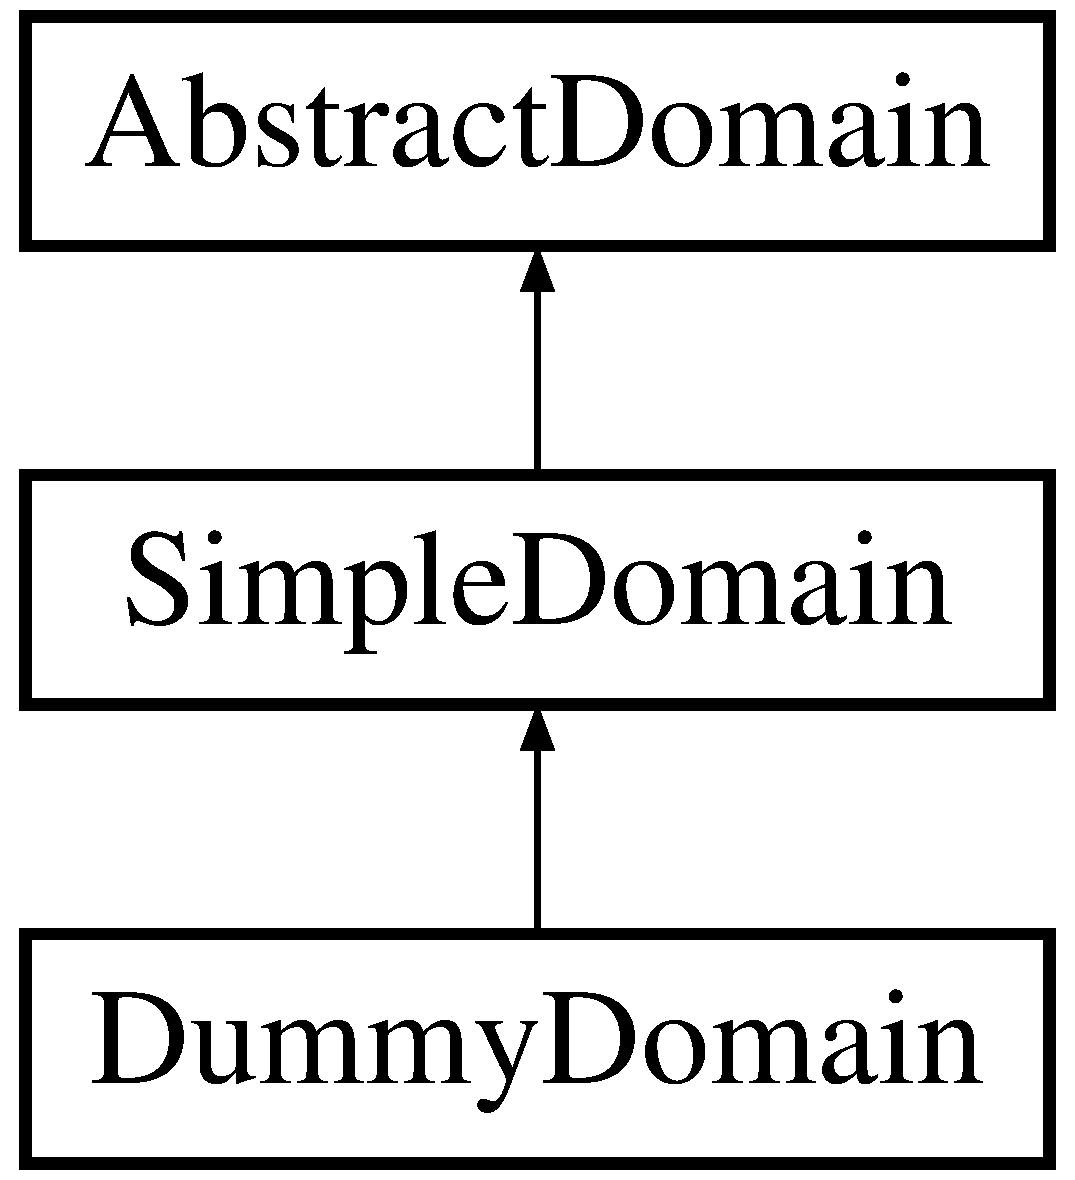
\includegraphics[height=3.000000cm]{class_dummy_domain}
\end{center}
\end{figure}
\subsection*{Public Member Functions}
\begin{DoxyCompactItemize}
\item 
\mbox{\hyperlink{class_dummy_domain_a19d6dde5b2f9be766cf2b838fac1f3bb}{Dummy\+Domain}} (string filename, vector$<$ \mbox{\hyperlink{structpoint}{point}} $>$ points)
\item 
virtual \mbox{\hyperlink{structpoint}{point}} \mbox{\hyperlink{class_dummy_domain_a72074e5e3e53028ec4b73bffee1ba229}{get\+Random\+Point}} ()
\end{DoxyCompactItemize}
\subsection*{Additional Inherited Members}


\subsection{Detailed Description}
Creates a Domain that does not generate random points, instead it loads them from the constructor call. 

\subsection{Constructor \& Destructor Documentation}
\mbox{\Hypertarget{class_dummy_domain_a19d6dde5b2f9be766cf2b838fac1f3bb}\label{class_dummy_domain_a19d6dde5b2f9be766cf2b838fac1f3bb}} 
\index{Dummy\+Domain@{Dummy\+Domain}!Dummy\+Domain@{Dummy\+Domain}}
\index{Dummy\+Domain@{Dummy\+Domain}!Dummy\+Domain@{Dummy\+Domain}}
\subsubsection{\texorpdfstring{Dummy\+Domain()}{DummyDomain()}}
{\footnotesize\ttfamily Dummy\+Domain\+::\+Dummy\+Domain (\begin{DoxyParamCaption}\item[{string}]{filename,  }\item[{vector$<$ \mbox{\hyperlink{structpoint}{point}} $>$}]{points }\end{DoxyParamCaption})}

Creates a domain with the geometry of the file
\begin{DoxyParams}{Parameters}
{\em filename} & with the fixed random points\\
\hline
{\em points.} & \\
\hline
{\em filename} & V\+TP file containing the geometry for the domain. \\
\hline
{\em points} & Points used for the tree generation. \\
\hline
\end{DoxyParams}


\subsection{Member Function Documentation}
\mbox{\Hypertarget{class_dummy_domain_a72074e5e3e53028ec4b73bffee1ba229}\label{class_dummy_domain_a72074e5e3e53028ec4b73bffee1ba229}} 
\index{Dummy\+Domain@{Dummy\+Domain}!get\+Random\+Point@{get\+Random\+Point}}
\index{get\+Random\+Point@{get\+Random\+Point}!Dummy\+Domain@{Dummy\+Domain}}
\subsubsection{\texorpdfstring{get\+Random\+Point()}{getRandomPoint()}}
{\footnotesize\ttfamily \mbox{\hyperlink{structpoint}{point}} Dummy\+Domain\+::get\+Random\+Point (\begin{DoxyParamCaption}{ }\end{DoxyParamCaption})\hspace{0.3cm}{\ttfamily [virtual]}}

Returns the first random point and removes it from the domain. \begin{DoxyReturn}{Returns}

\end{DoxyReturn}


Reimplemented from \mbox{\hyperlink{class_simple_domain}{Simple\+Domain}}.



The documentation for this class was generated from the following files\+:\begin{DoxyCompactItemize}
\item 
structures/domain/Dummy\+Domain.\+h\item 
structures/domain/Dummy\+Domain.\+cpp\end{DoxyCompactItemize}

\hypertarget{class_fixed_perfusion_radius_tree_generator}{}\section{Fixed\+Perfusion\+Radius\+Tree\+Generator Class Reference}
\label{class_fixed_perfusion_radius_tree_generator}\index{Fixed\+Perfusion\+Radius\+Tree\+Generator@{Fixed\+Perfusion\+Radius\+Tree\+Generator}}


{\ttfamily \#include $<$Fixed\+Perfusion\+Radius\+Tree\+Generator.\+h$>$}

Inheritance diagram for Fixed\+Perfusion\+Radius\+Tree\+Generator\+:\begin{figure}[H]
\begin{center}
\leavevmode
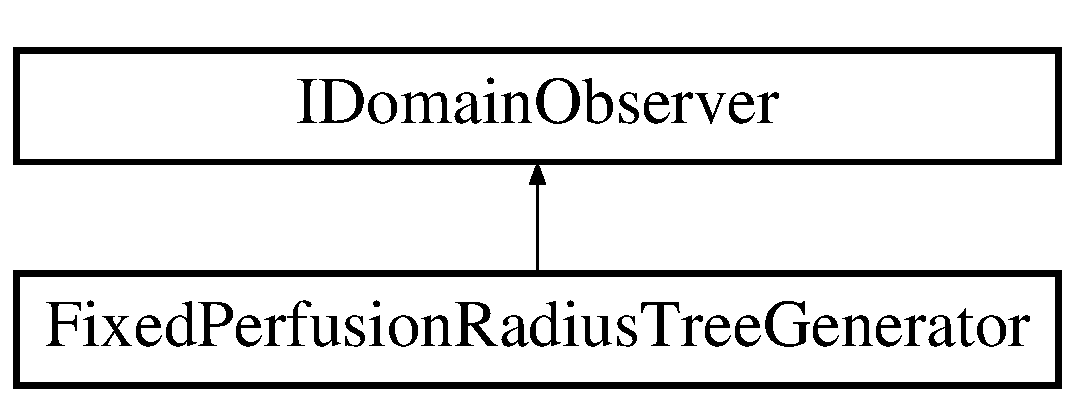
\includegraphics[height=2.000000cm]{d4/dce/class_fixed_perfusion_radius_tree_generator}
\end{center}
\end{figure}
\subsection*{Public Member Functions}
\begin{DoxyCompactItemize}
\item 
\hyperlink{class_fixed_perfusion_radius_tree_generator_a970125bd4e62f257d646c0ef3e0e7db6}{Fixed\+Perfusion\+Radius\+Tree\+Generator} (\hyperlink{class_abstract_domain}{Abstract\+Domain} $\ast$\hyperlink{class_fixed_perfusion_radius_tree_generator_a3f613d457aa40ecbec9c61b0fd559764}{domain}, \hyperlink{structpoint}{point} xi, double root\+Radii, double qi, long long int n\+Term, \hyperlink{class_abstract_constraint_function}{Abstract\+Constraint\+Function}$<$ double, int $>$ $\ast$gam, \hyperlink{class_abstract_constraint_function}{Abstract\+Constraint\+Function}$<$ double, int $>$ $\ast$eps\+Lim, \hyperlink{class_abstract_constraint_function}{Abstract\+Constraint\+Function}$<$ double, int $>$ $\ast$nu, double min\+Angle, double ref\+Pressure)
\item 
\hyperlink{class_fixed_perfusion_radius_tree_generator_a00a16101933078dfdcf037ef149348d9}{Fixed\+Perfusion\+Radius\+Tree\+Generator} (\hyperlink{class_abstract_domain}{Abstract\+Domain} $\ast$\hyperlink{class_fixed_perfusion_radius_tree_generator_a3f613d457aa40ecbec9c61b0fd559764}{domain}, \hyperlink{structpoint}{point} xi, double root\+Radii, double qi, long long int n\+Term, \hyperlink{class_abstract_constraint_function}{Abstract\+Constraint\+Function}$<$ double, int $>$ $\ast$gam, \hyperlink{class_abstract_constraint_function}{Abstract\+Constraint\+Function}$<$ double, int $>$ $\ast$eps\+Lim, \hyperlink{class_abstract_constraint_function}{Abstract\+Constraint\+Function}$<$ double, int $>$ $\ast$nu, double min\+Angle, double ref\+Pressure, double viscosity\+Tolerance, int optimized)
\item 
\hyperlink{class_fixed_perfusion_radius_tree_generator_a415ddd819e62f818b91bc40612ba1a7f}{Fixed\+Perfusion\+Radius\+Tree\+Generator} (\hyperlink{class_abstract_domain}{Abstract\+Domain} $\ast$\hyperlink{class_fixed_perfusion_radius_tree_generator_a3f613d457aa40ecbec9c61b0fd559764}{domain}, \hyperlink{class_abstract_structured_c_c_o_tree}{Abstract\+Structured\+C\+C\+O\+Tree} $\ast$\hyperlink{class_fixed_perfusion_radius_tree_generator_a79a3059e0c4555a2008829d5a51803dd}{tree}, long long int n\+Term, \hyperlink{class_abstract_constraint_function}{Abstract\+Constraint\+Function}$<$ double, int $>$ $\ast$gam, \hyperlink{class_abstract_constraint_function}{Abstract\+Constraint\+Function}$<$ double, int $>$ $\ast$eps\+Lim, \hyperlink{class_abstract_constraint_function}{Abstract\+Constraint\+Function}$<$ double, int $>$ $\ast$nu)
\item 
\hyperlink{class_abstract_structured_c_c_o_tree}{Abstract\+Structured\+C\+C\+O\+Tree} $\ast$ \hyperlink{class_fixed_perfusion_radius_tree_generator_abfe5fdcf60f2a7b2b900ae493a882ea4}{generate} ()
\item 
\hyperlink{class_abstract_structured_c_c_o_tree}{Abstract\+Structured\+C\+C\+O\+Tree} $\ast$ \hyperlink{class_fixed_perfusion_radius_tree_generator_a9feeb40ddba160de4499f435b129dc83}{resume} ()
\item 
\hyperlink{class_abstract_domain}{Abstract\+Domain} $\ast$ \hyperlink{class_fixed_perfusion_radius_tree_generator_ab5f60bf11b980a83faccdd3a667c6bf0}{get\+Domain} ()
\item 
vector$<$ \hyperlink{class_abstract_structured_c_c_o_tree}{Abstract\+Structured\+C\+C\+O\+Tree} $\ast$ $>$ \hyperlink{class_fixed_perfusion_radius_tree_generator_a5964f771575677452fbae6c21a7470e6}{get\+Trees} ()
\item 
void \hyperlink{class_fixed_perfusion_radius_tree_generator_a6aee969aaac8fc014accbb360d4fd306}{enable\+Configuration\+File} (string filename)
\item 
void \hyperlink{class_fixed_perfusion_radius_tree_generator_add5bd06f4fe8a15529084f6d78e71b44}{observable\+Modified} (\hyperlink{class_i_domain_observable}{I\+Domain\+Observable} $\ast$observable\+Instance)
\end{DoxyCompactItemize}
\subsection*{Protected Member Functions}
\begin{DoxyCompactItemize}
\item 
int \hyperlink{class_fixed_perfusion_radius_tree_generator_ae7a7f4b87282f81b141377032a537e08}{is\+Valid\+Root\+Segment} (\hyperlink{structpoint}{point} x\+New, int i\+Try)
\item 
int \hyperlink{class_fixed_perfusion_radius_tree_generator_a306a08e5b09ced0a19fcfae49c7e7399}{is\+Valid\+Segment} (\hyperlink{structpoint}{point} x\+New, int i\+Try)
\item 
void \hyperlink{class_fixed_perfusion_radius_tree_generator_a091f126a38dd910df10b81d7c8dee4b9}{generates\+Configuration\+File} (ios\+::openmode mode)
\item 
void \hyperlink{class_fixed_perfusion_radius_tree_generator_af82dbe3c22454f0b1e09be7e77ac8118}{mark\+Timestamp\+On\+Configuration\+File} (string label)
\item 
void \hyperlink{class_fixed_perfusion_radius_tree_generator_aa705213dee8c0e4679cae60d05510ffc}{close\+Configuration\+File} ()
\end{DoxyCompactItemize}
\subsection*{Protected Attributes}
\begin{DoxyCompactItemize}
\item 
ofstream \hyperlink{class_fixed_perfusion_radius_tree_generator_acccbb50a7aa221b58e80e47515650a5a}{conf\+File}
\item 
chrono\+::steady\+\_\+clock\+::time\+\_\+point \hyperlink{class_fixed_perfusion_radius_tree_generator_ab1945f73c7d8ac571c34b68792d5d317}{beginning\+Time}
\end{DoxyCompactItemize}
\subsection*{Private Attributes}
\begin{DoxyCompactItemize}
\item 
\hyperlink{class_generator_data}{Generator\+Data} $\ast$ \hyperlink{class_fixed_perfusion_radius_tree_generator_a00f2d253632c5188a13576d614586d02}{instance\+Data}
\item 
\hyperlink{class_generator_data_monitor}{Generator\+Data\+Monitor} $\ast$ \hyperlink{class_fixed_perfusion_radius_tree_generator_a431e0e44437bc9cbee263ab316c8ed60}{data\+Monitor}
\item 
long long int \hyperlink{class_fixed_perfusion_radius_tree_generator_a7f47f9518335cd88504f2575d75a6935}{n\+Terminals}
\item 
double \hyperlink{class_fixed_perfusion_radius_tree_generator_ae14a2fd89b3e87d51d8d304abab238be}{d\+Lim}
\item 
\hyperlink{class_abstract_domain}{Abstract\+Domain} $\ast$ \hyperlink{class_fixed_perfusion_radius_tree_generator_a3f613d457aa40ecbec9c61b0fd559764}{domain}
\item 
\hyperlink{class_abstract_structured_c_c_o_tree}{Abstract\+Structured\+C\+C\+O\+Tree} $\ast$ \hyperlink{class_fixed_perfusion_radius_tree_generator_a79a3059e0c4555a2008829d5a51803dd}{tree}
\item 
int \hyperlink{class_fixed_perfusion_radius_tree_generator_aa4e8b9db77041b6981d1747835faaafe}{is\+Generating\+Conf\+File}
\item 
string \hyperlink{class_fixed_perfusion_radius_tree_generator_a429c60ad818d28d0a50167beaecf60b9}{conf\+Filename}
\end{DoxyCompactItemize}


\subsection{Detailed Description}
Generator for a single fixed perfusion tree. 

\subsection{Constructor \& Destructor Documentation}
\index{Fixed\+Perfusion\+Radius\+Tree\+Generator@{Fixed\+Perfusion\+Radius\+Tree\+Generator}!Fixed\+Perfusion\+Radius\+Tree\+Generator@{Fixed\+Perfusion\+Radius\+Tree\+Generator}}
\index{Fixed\+Perfusion\+Radius\+Tree\+Generator@{Fixed\+Perfusion\+Radius\+Tree\+Generator}!Fixed\+Perfusion\+Radius\+Tree\+Generator@{Fixed\+Perfusion\+Radius\+Tree\+Generator}}
\subsubsection[{\texorpdfstring{Fixed\+Perfusion\+Radius\+Tree\+Generator(\+Abstract\+Domain $\ast$domain, point xi, double root\+Radii, double qi, long long int n\+Term, Abstract\+Constraint\+Function$<$ double, int $>$ $\ast$gam, Abstract\+Constraint\+Function$<$ double, int $>$ $\ast$eps\+Lim, Abstract\+Constraint\+Function$<$ double, int $>$ $\ast$nu, double min\+Angle, double ref\+Pressure)}{FixedPerfusionRadiusTreeGenerator(AbstractDomain *domain, point xi, double rootRadii, double qi, long long int nTerm, AbstractConstraintFunction< double, int > *gam, AbstractConstraintFunction< double, int > *epsLim, AbstractConstraintFunction< double, int > *nu, double minAngle, double refPressure)}}]{\setlength{\rightskip}{0pt plus 5cm}Fixed\+Perfusion\+Radius\+Tree\+Generator\+::\+Fixed\+Perfusion\+Radius\+Tree\+Generator (
\begin{DoxyParamCaption}
\item[{{\bf Abstract\+Domain} $\ast$}]{domain, }
\item[{{\bf point}}]{xi, }
\item[{double}]{root\+Radii, }
\item[{double}]{qi, }
\item[{long long int}]{n\+Term, }
\item[{{\bf Abstract\+Constraint\+Function}$<$ double, int $>$ $\ast$}]{gam, }
\item[{{\bf Abstract\+Constraint\+Function}$<$ double, int $>$ $\ast$}]{eps\+Lim, }
\item[{{\bf Abstract\+Constraint\+Function}$<$ double, int $>$ $\ast$}]{nu, }
\item[{double}]{min\+Angle, }
\item[{double}]{ref\+Pressure}
\end{DoxyParamCaption}
)}\hypertarget{class_fixed_perfusion_radius_tree_generator_a970125bd4e62f257d646c0ef3e0e7db6}{}\label{class_fixed_perfusion_radius_tree_generator_a970125bd4e62f257d646c0ef3e0e7db6}
Constructor for non-\/optimized and constant viscosity tree. 
\begin{DoxyParams}{Parameters}
{\em domain} & Perfusion domain. \\
\hline
{\em xi} & Root proximal position. \\
\hline
{\em root\+Radii} & Root radius. \\
\hline
{\em qi} & Inflow for the perfusion domain. \\
\hline
{\em n\+Term} & Total number of tree terminals. \\
\hline
{\em gam} & Murray\textquotesingle{}s power law function. \\
\hline
{\em eps\+Lim} & Symmetry constraint function. \\
\hline
{\em nu} & Viscosity function. \\
\hline
{\em min\+Angle} & Minimum allowed bifurcation angle. \\
\hline
\end{DoxyParams}
\index{Fixed\+Perfusion\+Radius\+Tree\+Generator@{Fixed\+Perfusion\+Radius\+Tree\+Generator}!Fixed\+Perfusion\+Radius\+Tree\+Generator@{Fixed\+Perfusion\+Radius\+Tree\+Generator}}
\index{Fixed\+Perfusion\+Radius\+Tree\+Generator@{Fixed\+Perfusion\+Radius\+Tree\+Generator}!Fixed\+Perfusion\+Radius\+Tree\+Generator@{Fixed\+Perfusion\+Radius\+Tree\+Generator}}
\subsubsection[{\texorpdfstring{Fixed\+Perfusion\+Radius\+Tree\+Generator(\+Abstract\+Domain $\ast$domain, point xi, double root\+Radii, double qi, long long int n\+Term, Abstract\+Constraint\+Function$<$ double, int $>$ $\ast$gam, Abstract\+Constraint\+Function$<$ double, int $>$ $\ast$eps\+Lim, Abstract\+Constraint\+Function$<$ double, int $>$ $\ast$nu, double min\+Angle, double ref\+Pressure, double viscosity\+Tolerance, int optimized)}{FixedPerfusionRadiusTreeGenerator(AbstractDomain *domain, point xi, double rootRadii, double qi, long long int nTerm, AbstractConstraintFunction< double, int > *gam, AbstractConstraintFunction< double, int > *epsLim, AbstractConstraintFunction< double, int > *nu, double minAngle, double refPressure, double viscosityTolerance, int optimized)}}]{\setlength{\rightskip}{0pt plus 5cm}Fixed\+Perfusion\+Radius\+Tree\+Generator\+::\+Fixed\+Perfusion\+Radius\+Tree\+Generator (
\begin{DoxyParamCaption}
\item[{{\bf Abstract\+Domain} $\ast$}]{domain, }
\item[{{\bf point}}]{xi, }
\item[{double}]{root\+Radii, }
\item[{double}]{qi, }
\item[{long long int}]{n\+Term, }
\item[{{\bf Abstract\+Constraint\+Function}$<$ double, int $>$ $\ast$}]{gam, }
\item[{{\bf Abstract\+Constraint\+Function}$<$ double, int $>$ $\ast$}]{eps\+Lim, }
\item[{{\bf Abstract\+Constraint\+Function}$<$ double, int $>$ $\ast$}]{nu, }
\item[{double}]{min\+Angle, }
\item[{double}]{ref\+Pressure, }
\item[{double}]{viscosity\+Tolerance, }
\item[{int}]{optimized}
\end{DoxyParamCaption}
)}\hypertarget{class_fixed_perfusion_radius_tree_generator_a00a16101933078dfdcf037ef149348d9}{}\label{class_fixed_perfusion_radius_tree_generator_a00a16101933078dfdcf037ef149348d9}
Constructor for tree with Fahraeus-\/\+Lindquist viscosity model. 
\begin{DoxyParams}{Parameters}
{\em domain} & Perfusion domain. \\
\hline
{\em xi} & Root proximal position. \\
\hline
{\em root\+Radii} & Root radius. \\
\hline
{\em qi} & Inflow for the perfusion domain. \\
\hline
{\em n\+Term} & Total number of tree terminals. \\
\hline
{\em gam} & Murray\textquotesingle{}s power law function. \\
\hline
{\em eps\+Lim} & Symmetry constraint function. \\
\hline
{\em nu} & Viscosity function. \\
\hline
{\em min\+Angle} & Minimum allowed bifurcation angle. \\
\hline
{\em viscosity\+Tolerance} & Convergence tolerance for the absolute beta variation in the viscosity iterative scheme. \\
\hline
{\em optimized} & If it is optimized with partial tree scaling. \\
\hline
\end{DoxyParams}
\index{Fixed\+Perfusion\+Radius\+Tree\+Generator@{Fixed\+Perfusion\+Radius\+Tree\+Generator}!Fixed\+Perfusion\+Radius\+Tree\+Generator@{Fixed\+Perfusion\+Radius\+Tree\+Generator}}
\index{Fixed\+Perfusion\+Radius\+Tree\+Generator@{Fixed\+Perfusion\+Radius\+Tree\+Generator}!Fixed\+Perfusion\+Radius\+Tree\+Generator@{Fixed\+Perfusion\+Radius\+Tree\+Generator}}
\subsubsection[{\texorpdfstring{Fixed\+Perfusion\+Radius\+Tree\+Generator(\+Abstract\+Domain $\ast$domain, Abstract\+Structured\+C\+C\+O\+Tree $\ast$tree, long long int n\+Term, Abstract\+Constraint\+Function$<$ double, int $>$ $\ast$gam, Abstract\+Constraint\+Function$<$ double, int $>$ $\ast$eps\+Lim, Abstract\+Constraint\+Function$<$ double, int $>$ $\ast$nu)}{FixedPerfusionRadiusTreeGenerator(AbstractDomain *domain, AbstractStructuredCCOTree *tree, long long int nTerm, AbstractConstraintFunction< double, int > *gam, AbstractConstraintFunction< double, int > *epsLim, AbstractConstraintFunction< double, int > *nu)}}]{\setlength{\rightskip}{0pt plus 5cm}Fixed\+Perfusion\+Radius\+Tree\+Generator\+::\+Fixed\+Perfusion\+Radius\+Tree\+Generator (
\begin{DoxyParamCaption}
\item[{{\bf Abstract\+Domain} $\ast$}]{domain, }
\item[{{\bf Abstract\+Structured\+C\+C\+O\+Tree} $\ast$}]{tree, }
\item[{long long int}]{n\+Term, }
\item[{{\bf Abstract\+Constraint\+Function}$<$ double, int $>$ $\ast$}]{gam, }
\item[{{\bf Abstract\+Constraint\+Function}$<$ double, int $>$ $\ast$}]{eps\+Lim, }
\item[{{\bf Abstract\+Constraint\+Function}$<$ double, int $>$ $\ast$}]{nu}
\end{DoxyParamCaption}
)}\hypertarget{class_fixed_perfusion_radius_tree_generator_a415ddd819e62f818b91bc40612ba1a7f}{}\label{class_fixed_perfusion_radius_tree_generator_a415ddd819e62f818b91bc40612ba1a7f}
Constructor to resume from a pre-\/existent tree. 
\begin{DoxyParams}{Parameters}
{\em domain} & Perfusion domain. \\
\hline
{\em tree} & Pre-\/existent tree. \\
\hline
{\em n\+Term} & Total number of tree terminals. \\
\hline
{\em gam} & Murray\textquotesingle{}s power law function. \\
\hline
{\em eps\+Lim} & Symmetry constraint function. \\
\hline
{\em nu} & Viscosity function. \\
\hline
\end{DoxyParams}


\subsection{Member Function Documentation}
\index{Fixed\+Perfusion\+Radius\+Tree\+Generator@{Fixed\+Perfusion\+Radius\+Tree\+Generator}!close\+Configuration\+File@{close\+Configuration\+File}}
\index{close\+Configuration\+File@{close\+Configuration\+File}!Fixed\+Perfusion\+Radius\+Tree\+Generator@{Fixed\+Perfusion\+Radius\+Tree\+Generator}}
\subsubsection[{\texorpdfstring{close\+Configuration\+File()}{closeConfigurationFile()}}]{\setlength{\rightskip}{0pt plus 5cm}void Fixed\+Perfusion\+Radius\+Tree\+Generator\+::close\+Configuration\+File (
\begin{DoxyParamCaption}
{}
\end{DoxyParamCaption}
)\hspace{0.3cm}{\ttfamily [protected]}}\hypertarget{class_fixed_perfusion_radius_tree_generator_aa705213dee8c0e4679cae60d05510ffc}{}\label{class_fixed_perfusion_radius_tree_generator_aa705213dee8c0e4679cae60d05510ffc}
Closes the configuration file for the current tree generation. \index{Fixed\+Perfusion\+Radius\+Tree\+Generator@{Fixed\+Perfusion\+Radius\+Tree\+Generator}!enable\+Configuration\+File@{enable\+Configuration\+File}}
\index{enable\+Configuration\+File@{enable\+Configuration\+File}!Fixed\+Perfusion\+Radius\+Tree\+Generator@{Fixed\+Perfusion\+Radius\+Tree\+Generator}}
\subsubsection[{\texorpdfstring{enable\+Configuration\+File(string filename)}{enableConfigurationFile(string filename)}}]{\setlength{\rightskip}{0pt plus 5cm}void Fixed\+Perfusion\+Radius\+Tree\+Generator\+::enable\+Configuration\+File (
\begin{DoxyParamCaption}
\item[{string}]{filename}
\end{DoxyParamCaption}
)}\hypertarget{class_fixed_perfusion_radius_tree_generator_a6aee969aaac8fc014accbb360d4fd306}{}\label{class_fixed_perfusion_radius_tree_generator_a6aee969aaac8fc014accbb360d4fd306}
Enables the configuration file generation capabilities. 
\begin{DoxyParams}{Parameters}
{\em filename} & File name where the generator stores the configuration data. \\
\hline
\end{DoxyParams}
\index{Fixed\+Perfusion\+Radius\+Tree\+Generator@{Fixed\+Perfusion\+Radius\+Tree\+Generator}!generate@{generate}}
\index{generate@{generate}!Fixed\+Perfusion\+Radius\+Tree\+Generator@{Fixed\+Perfusion\+Radius\+Tree\+Generator}}
\subsubsection[{\texorpdfstring{generate()}{generate()}}]{\setlength{\rightskip}{0pt plus 5cm}{\bf Abstract\+Structured\+C\+C\+O\+Tree} $\ast$ Fixed\+Perfusion\+Radius\+Tree\+Generator\+::generate (
\begin{DoxyParamCaption}
{}
\end{DoxyParamCaption}
)}\hypertarget{class_fixed_perfusion_radius_tree_generator_abfe5fdcf60f2a7b2b900ae493a882ea4}{}\label{class_fixed_perfusion_radius_tree_generator_abfe5fdcf60f2a7b2b900ae493a882ea4}
Generates the specified tree. \begin{DoxyReturn}{Returns}
Perfusion tree. 
\end{DoxyReturn}
\index{Fixed\+Perfusion\+Radius\+Tree\+Generator@{Fixed\+Perfusion\+Radius\+Tree\+Generator}!generates\+Configuration\+File@{generates\+Configuration\+File}}
\index{generates\+Configuration\+File@{generates\+Configuration\+File}!Fixed\+Perfusion\+Radius\+Tree\+Generator@{Fixed\+Perfusion\+Radius\+Tree\+Generator}}
\subsubsection[{\texorpdfstring{generates\+Configuration\+File(ios\+::openmode mode)}{generatesConfigurationFile(ios::openmode mode)}}]{\setlength{\rightskip}{0pt plus 5cm}void Fixed\+Perfusion\+Radius\+Tree\+Generator\+::generates\+Configuration\+File (
\begin{DoxyParamCaption}
\item[{ios\+::openmode}]{mode}
\end{DoxyParamCaption}
)\hspace{0.3cm}{\ttfamily [protected]}}\hypertarget{class_fixed_perfusion_radius_tree_generator_a091f126a38dd910df10b81d7c8dee4b9}{}\label{class_fixed_perfusion_radius_tree_generator_a091f126a38dd910df10b81d7c8dee4b9}
Generates the configuration file for the current tree generation. 
\begin{DoxyParams}{Parameters}
{\em mode} & Is the openmode used for the generated file (ios\+::out for generation, ios\+::app for resume). \\
\hline
\end{DoxyParams}
\index{Fixed\+Perfusion\+Radius\+Tree\+Generator@{Fixed\+Perfusion\+Radius\+Tree\+Generator}!get\+Domain@{get\+Domain}}
\index{get\+Domain@{get\+Domain}!Fixed\+Perfusion\+Radius\+Tree\+Generator@{Fixed\+Perfusion\+Radius\+Tree\+Generator}}
\subsubsection[{\texorpdfstring{get\+Domain()}{getDomain()}}]{\setlength{\rightskip}{0pt plus 5cm}{\bf Abstract\+Domain} $\ast$ Fixed\+Perfusion\+Radius\+Tree\+Generator\+::get\+Domain (
\begin{DoxyParamCaption}
{}
\end{DoxyParamCaption}
)}\hypertarget{class_fixed_perfusion_radius_tree_generator_ab5f60bf11b980a83faccdd3a667c6bf0}{}\label{class_fixed_perfusion_radius_tree_generator_ab5f60bf11b980a83faccdd3a667c6bf0}
Returns the perfusion domain. \begin{DoxyReturn}{Returns}
Perfusion domain. 
\end{DoxyReturn}
\index{Fixed\+Perfusion\+Radius\+Tree\+Generator@{Fixed\+Perfusion\+Radius\+Tree\+Generator}!get\+Trees@{get\+Trees}}
\index{get\+Trees@{get\+Trees}!Fixed\+Perfusion\+Radius\+Tree\+Generator@{Fixed\+Perfusion\+Radius\+Tree\+Generator}}
\subsubsection[{\texorpdfstring{get\+Trees()}{getTrees()}}]{\setlength{\rightskip}{0pt plus 5cm}vector$<$ {\bf Abstract\+Structured\+C\+C\+O\+Tree} $\ast$ $>$ Fixed\+Perfusion\+Radius\+Tree\+Generator\+::get\+Trees (
\begin{DoxyParamCaption}
{}
\end{DoxyParamCaption}
)}\hypertarget{class_fixed_perfusion_radius_tree_generator_a5964f771575677452fbae6c21a7470e6}{}\label{class_fixed_perfusion_radius_tree_generator_a5964f771575677452fbae6c21a7470e6}
Returns the generated tree. \begin{DoxyReturn}{Returns}
Generated tree. 
\end{DoxyReturn}
\index{Fixed\+Perfusion\+Radius\+Tree\+Generator@{Fixed\+Perfusion\+Radius\+Tree\+Generator}!is\+Valid\+Root\+Segment@{is\+Valid\+Root\+Segment}}
\index{is\+Valid\+Root\+Segment@{is\+Valid\+Root\+Segment}!Fixed\+Perfusion\+Radius\+Tree\+Generator@{Fixed\+Perfusion\+Radius\+Tree\+Generator}}
\subsubsection[{\texorpdfstring{is\+Valid\+Root\+Segment(point x\+New, int i\+Try)}{isValidRootSegment(point xNew, int iTry)}}]{\setlength{\rightskip}{0pt plus 5cm}int Fixed\+Perfusion\+Radius\+Tree\+Generator\+::is\+Valid\+Root\+Segment (
\begin{DoxyParamCaption}
\item[{{\bf point}}]{x\+New, }
\item[{int}]{i\+Try}
\end{DoxyParamCaption}
)\hspace{0.3cm}{\ttfamily [protected]}}\hypertarget{class_fixed_perfusion_radius_tree_generator_ae7a7f4b87282f81b141377032a537e08}{}\label{class_fixed_perfusion_radius_tree_generator_ae7a7f4b87282f81b141377032a537e08}
Returns if the length of the segment defined by x\+Prox and x\+New is higher than d\+Lim (distance criterion). 
\begin{DoxyParams}{Parameters}
{\em x\+New} & Proposed distal point. \\
\hline
{\em i\+Try} & Number of trial. \\
\hline
\end{DoxyParams}
\begin{DoxyReturn}{Returns}
If the root segment is valid. 
\end{DoxyReturn}
\index{Fixed\+Perfusion\+Radius\+Tree\+Generator@{Fixed\+Perfusion\+Radius\+Tree\+Generator}!is\+Valid\+Segment@{is\+Valid\+Segment}}
\index{is\+Valid\+Segment@{is\+Valid\+Segment}!Fixed\+Perfusion\+Radius\+Tree\+Generator@{Fixed\+Perfusion\+Radius\+Tree\+Generator}}
\subsubsection[{\texorpdfstring{is\+Valid\+Segment(point x\+New, int i\+Try)}{isValidSegment(point xNew, int iTry)}}]{\setlength{\rightskip}{0pt plus 5cm}int Fixed\+Perfusion\+Radius\+Tree\+Generator\+::is\+Valid\+Segment (
\begin{DoxyParamCaption}
\item[{{\bf point}}]{x\+New, }
\item[{int}]{i\+Try}
\end{DoxyParamCaption}
)\hspace{0.3cm}{\ttfamily [protected]}}\hypertarget{class_fixed_perfusion_radius_tree_generator_a306a08e5b09ced0a19fcfae49c7e7399}{}\label{class_fixed_perfusion_radius_tree_generator_a306a08e5b09ced0a19fcfae49c7e7399}
Returns if the closest point to the whole try is greater than d\+Lim (distance criterion for a new segment). 
\begin{DoxyParams}{Parameters}
{\em x\+New} & Proposed distal point. \\
\hline
{\em i\+Try} & Number of trial. \\
\hline
\end{DoxyParams}
\begin{DoxyReturn}{Returns}
If the segment is valid. 
\end{DoxyReturn}
\index{Fixed\+Perfusion\+Radius\+Tree\+Generator@{Fixed\+Perfusion\+Radius\+Tree\+Generator}!mark\+Timestamp\+On\+Configuration\+File@{mark\+Timestamp\+On\+Configuration\+File}}
\index{mark\+Timestamp\+On\+Configuration\+File@{mark\+Timestamp\+On\+Configuration\+File}!Fixed\+Perfusion\+Radius\+Tree\+Generator@{Fixed\+Perfusion\+Radius\+Tree\+Generator}}
\subsubsection[{\texorpdfstring{mark\+Timestamp\+On\+Configuration\+File(string label)}{markTimestampOnConfigurationFile(string label)}}]{\setlength{\rightskip}{0pt plus 5cm}void Fixed\+Perfusion\+Radius\+Tree\+Generator\+::mark\+Timestamp\+On\+Configuration\+File (
\begin{DoxyParamCaption}
\item[{string}]{label}
\end{DoxyParamCaption}
)\hspace{0.3cm}{\ttfamily [protected]}}\hypertarget{class_fixed_perfusion_radius_tree_generator_af82dbe3c22454f0b1e09be7e77ac8118}{}\label{class_fixed_perfusion_radius_tree_generator_af82dbe3c22454f0b1e09be7e77ac8118}
Saves the timestamp for event {\ttfamily label}. \index{Fixed\+Perfusion\+Radius\+Tree\+Generator@{Fixed\+Perfusion\+Radius\+Tree\+Generator}!observable\+Modified@{observable\+Modified}}
\index{observable\+Modified@{observable\+Modified}!Fixed\+Perfusion\+Radius\+Tree\+Generator@{Fixed\+Perfusion\+Radius\+Tree\+Generator}}
\subsubsection[{\texorpdfstring{observable\+Modified(\+I\+Domain\+Observable $\ast$observable\+Instance)}{observableModified(IDomainObservable *observableInstance)}}]{\setlength{\rightskip}{0pt plus 5cm}void Fixed\+Perfusion\+Radius\+Tree\+Generator\+::observable\+Modified (
\begin{DoxyParamCaption}
\item[{{\bf I\+Domain\+Observable} $\ast$}]{observable\+Instance}
\end{DoxyParamCaption}
)\hspace{0.3cm}{\ttfamily [virtual]}}\hypertarget{class_fixed_perfusion_radius_tree_generator_add5bd06f4fe8a15529084f6d78e71b44}{}\label{class_fixed_perfusion_radius_tree_generator_add5bd06f4fe8a15529084f6d78e71b44}
Updates internal data from this instance after the domain has been modified. 
\begin{DoxyParams}{Parameters}
{\em observable\+Instance} & Domain instance modified. \\
\hline
\end{DoxyParams}


Implements \hyperlink{class_i_domain_observer_aee18640c20a6feaa16e4bf3bdde887a3}{I\+Domain\+Observer}.

\index{Fixed\+Perfusion\+Radius\+Tree\+Generator@{Fixed\+Perfusion\+Radius\+Tree\+Generator}!resume@{resume}}
\index{resume@{resume}!Fixed\+Perfusion\+Radius\+Tree\+Generator@{Fixed\+Perfusion\+Radius\+Tree\+Generator}}
\subsubsection[{\texorpdfstring{resume()}{resume()}}]{\setlength{\rightskip}{0pt plus 5cm}{\bf Abstract\+Structured\+C\+C\+O\+Tree} $\ast$ Fixed\+Perfusion\+Radius\+Tree\+Generator\+::resume (
\begin{DoxyParamCaption}
{}
\end{DoxyParamCaption}
)}\hypertarget{class_fixed_perfusion_radius_tree_generator_a9feeb40ddba160de4499f435b129dc83}{}\label{class_fixed_perfusion_radius_tree_generator_a9feeb40ddba160de4499f435b129dc83}
Resumes the tree generation. \begin{DoxyReturn}{Returns}
Perfusion tree. 
\end{DoxyReturn}


\subsection{Member Data Documentation}
\index{Fixed\+Perfusion\+Radius\+Tree\+Generator@{Fixed\+Perfusion\+Radius\+Tree\+Generator}!beginning\+Time@{beginning\+Time}}
\index{beginning\+Time@{beginning\+Time}!Fixed\+Perfusion\+Radius\+Tree\+Generator@{Fixed\+Perfusion\+Radius\+Tree\+Generator}}
\subsubsection[{\texorpdfstring{beginning\+Time}{beginningTime}}]{\setlength{\rightskip}{0pt plus 5cm}chrono\+::steady\+\_\+clock\+::time\+\_\+point Fixed\+Perfusion\+Radius\+Tree\+Generator\+::beginning\+Time\hspace{0.3cm}{\ttfamily [protected]}}\hypertarget{class_fixed_perfusion_radius_tree_generator_ab1945f73c7d8ac571c34b68792d5d317}{}\label{class_fixed_perfusion_radius_tree_generator_ab1945f73c7d8ac571c34b68792d5d317}
Initial timestamp of the generation process. \index{Fixed\+Perfusion\+Radius\+Tree\+Generator@{Fixed\+Perfusion\+Radius\+Tree\+Generator}!conf\+File@{conf\+File}}
\index{conf\+File@{conf\+File}!Fixed\+Perfusion\+Radius\+Tree\+Generator@{Fixed\+Perfusion\+Radius\+Tree\+Generator}}
\subsubsection[{\texorpdfstring{conf\+File}{confFile}}]{\setlength{\rightskip}{0pt plus 5cm}ofstream Fixed\+Perfusion\+Radius\+Tree\+Generator\+::conf\+File\hspace{0.3cm}{\ttfamily [protected]}}\hypertarget{class_fixed_perfusion_radius_tree_generator_acccbb50a7aa221b58e80e47515650a5a}{}\label{class_fixed_perfusion_radius_tree_generator_acccbb50a7aa221b58e80e47515650a5a}
Configuration file stream. \index{Fixed\+Perfusion\+Radius\+Tree\+Generator@{Fixed\+Perfusion\+Radius\+Tree\+Generator}!conf\+Filename@{conf\+Filename}}
\index{conf\+Filename@{conf\+Filename}!Fixed\+Perfusion\+Radius\+Tree\+Generator@{Fixed\+Perfusion\+Radius\+Tree\+Generator}}
\subsubsection[{\texorpdfstring{conf\+Filename}{confFilename}}]{\setlength{\rightskip}{0pt plus 5cm}string Fixed\+Perfusion\+Radius\+Tree\+Generator\+::conf\+Filename\hspace{0.3cm}{\ttfamily [private]}}\hypertarget{class_fixed_perfusion_radius_tree_generator_a429c60ad818d28d0a50167beaecf60b9}{}\label{class_fixed_perfusion_radius_tree_generator_a429c60ad818d28d0a50167beaecf60b9}
File name for the configuration file. \index{Fixed\+Perfusion\+Radius\+Tree\+Generator@{Fixed\+Perfusion\+Radius\+Tree\+Generator}!data\+Monitor@{data\+Monitor}}
\index{data\+Monitor@{data\+Monitor}!Fixed\+Perfusion\+Radius\+Tree\+Generator@{Fixed\+Perfusion\+Radius\+Tree\+Generator}}
\subsubsection[{\texorpdfstring{data\+Monitor}{dataMonitor}}]{\setlength{\rightskip}{0pt plus 5cm}{\bf Generator\+Data\+Monitor}$\ast$ Fixed\+Perfusion\+Radius\+Tree\+Generator\+::data\+Monitor\hspace{0.3cm}{\ttfamily [private]}}\hypertarget{class_fixed_perfusion_radius_tree_generator_a431e0e44437bc9cbee263ab316c8ed60}{}\label{class_fixed_perfusion_radius_tree_generator_a431e0e44437bc9cbee263ab316c8ed60}
Monitor of the {\ttfamily instance\+Data} . \index{Fixed\+Perfusion\+Radius\+Tree\+Generator@{Fixed\+Perfusion\+Radius\+Tree\+Generator}!d\+Lim@{d\+Lim}}
\index{d\+Lim@{d\+Lim}!Fixed\+Perfusion\+Radius\+Tree\+Generator@{Fixed\+Perfusion\+Radius\+Tree\+Generator}}
\subsubsection[{\texorpdfstring{d\+Lim}{dLim}}]{\setlength{\rightskip}{0pt plus 5cm}double Fixed\+Perfusion\+Radius\+Tree\+Generator\+::d\+Lim\hspace{0.3cm}{\ttfamily [private]}}\hypertarget{class_fixed_perfusion_radius_tree_generator_ae14a2fd89b3e87d51d8d304abab238be}{}\label{class_fixed_perfusion_radius_tree_generator_ae14a2fd89b3e87d51d8d304abab238be}
Perfusion volume. \index{Fixed\+Perfusion\+Radius\+Tree\+Generator@{Fixed\+Perfusion\+Radius\+Tree\+Generator}!domain@{domain}}
\index{domain@{domain}!Fixed\+Perfusion\+Radius\+Tree\+Generator@{Fixed\+Perfusion\+Radius\+Tree\+Generator}}
\subsubsection[{\texorpdfstring{domain}{domain}}]{\setlength{\rightskip}{0pt plus 5cm}{\bf Abstract\+Domain}$\ast$ Fixed\+Perfusion\+Radius\+Tree\+Generator\+::domain\hspace{0.3cm}{\ttfamily [private]}}\hypertarget{class_fixed_perfusion_radius_tree_generator_a3f613d457aa40ecbec9c61b0fd559764}{}\label{class_fixed_perfusion_radius_tree_generator_a3f613d457aa40ecbec9c61b0fd559764}
Perfusion domain. \index{Fixed\+Perfusion\+Radius\+Tree\+Generator@{Fixed\+Perfusion\+Radius\+Tree\+Generator}!instance\+Data@{instance\+Data}}
\index{instance\+Data@{instance\+Data}!Fixed\+Perfusion\+Radius\+Tree\+Generator@{Fixed\+Perfusion\+Radius\+Tree\+Generator}}
\subsubsection[{\texorpdfstring{instance\+Data}{instanceData}}]{\setlength{\rightskip}{0pt plus 5cm}{\bf Generator\+Data}$\ast$ Fixed\+Perfusion\+Radius\+Tree\+Generator\+::instance\+Data\hspace{0.3cm}{\ttfamily [private]}}\hypertarget{class_fixed_perfusion_radius_tree_generator_a00f2d253632c5188a13576d614586d02}{}\label{class_fixed_perfusion_radius_tree_generator_a00f2d253632c5188a13576d614586d02}
Wrapper with parameters associated to a tree generation process. \index{Fixed\+Perfusion\+Radius\+Tree\+Generator@{Fixed\+Perfusion\+Radius\+Tree\+Generator}!is\+Generating\+Conf\+File@{is\+Generating\+Conf\+File}}
\index{is\+Generating\+Conf\+File@{is\+Generating\+Conf\+File}!Fixed\+Perfusion\+Radius\+Tree\+Generator@{Fixed\+Perfusion\+Radius\+Tree\+Generator}}
\subsubsection[{\texorpdfstring{is\+Generating\+Conf\+File}{isGeneratingConfFile}}]{\setlength{\rightskip}{0pt plus 5cm}int Fixed\+Perfusion\+Radius\+Tree\+Generator\+::is\+Generating\+Conf\+File\hspace{0.3cm}{\ttfamily [private]}}\hypertarget{class_fixed_perfusion_radius_tree_generator_aa4e8b9db77041b6981d1747835faaafe}{}\label{class_fixed_perfusion_radius_tree_generator_aa4e8b9db77041b6981d1747835faaafe}
If the current generation saves the configuration used. \index{Fixed\+Perfusion\+Radius\+Tree\+Generator@{Fixed\+Perfusion\+Radius\+Tree\+Generator}!n\+Terminals@{n\+Terminals}}
\index{n\+Terminals@{n\+Terminals}!Fixed\+Perfusion\+Radius\+Tree\+Generator@{Fixed\+Perfusion\+Radius\+Tree\+Generator}}
\subsubsection[{\texorpdfstring{n\+Terminals}{nTerminals}}]{\setlength{\rightskip}{0pt plus 5cm}long long int Fixed\+Perfusion\+Radius\+Tree\+Generator\+::n\+Terminals\hspace{0.3cm}{\ttfamily [private]}}\hypertarget{class_fixed_perfusion_radius_tree_generator_a7f47f9518335cd88504f2575d75a6935}{}\label{class_fixed_perfusion_radius_tree_generator_a7f47f9518335cd88504f2575d75a6935}
Amount of terminals in the trees. \index{Fixed\+Perfusion\+Radius\+Tree\+Generator@{Fixed\+Perfusion\+Radius\+Tree\+Generator}!tree@{tree}}
\index{tree@{tree}!Fixed\+Perfusion\+Radius\+Tree\+Generator@{Fixed\+Perfusion\+Radius\+Tree\+Generator}}
\subsubsection[{\texorpdfstring{tree}{tree}}]{\setlength{\rightskip}{0pt plus 5cm}{\bf Abstract\+Structured\+C\+C\+O\+Tree}$\ast$ Fixed\+Perfusion\+Radius\+Tree\+Generator\+::tree\hspace{0.3cm}{\ttfamily [private]}}\hypertarget{class_fixed_perfusion_radius_tree_generator_a79a3059e0c4555a2008829d5a51803dd}{}\label{class_fixed_perfusion_radius_tree_generator_a79a3059e0c4555a2008829d5a51803dd}
Generated trees. 

The documentation for this class was generated from the following files\+:\begin{DoxyCompactItemize}
\item 
core/Fixed\+Perfusion\+Radius\+Tree\+Generator.\+h\item 
core/Fixed\+Perfusion\+Radius\+Tree\+Generator.\+cpp\end{DoxyCompactItemize}

\hypertarget{class_f_r_r_c_c_o_s_tree}{}\section{F\+R\+R\+C\+C\+O\+S\+Tree Class Reference}
\label{class_f_r_r_c_c_o_s_tree}\index{F\+R\+R\+C\+C\+O\+S\+Tree@{F\+R\+R\+C\+C\+O\+S\+Tree}}


{\ttfamily \#include $<$F\+R\+R\+C\+C\+O\+S\+Tree.\+h$>$}

Inheritance diagram for F\+R\+R\+C\+C\+O\+S\+Tree\+:\begin{figure}[H]
\begin{center}
\leavevmode
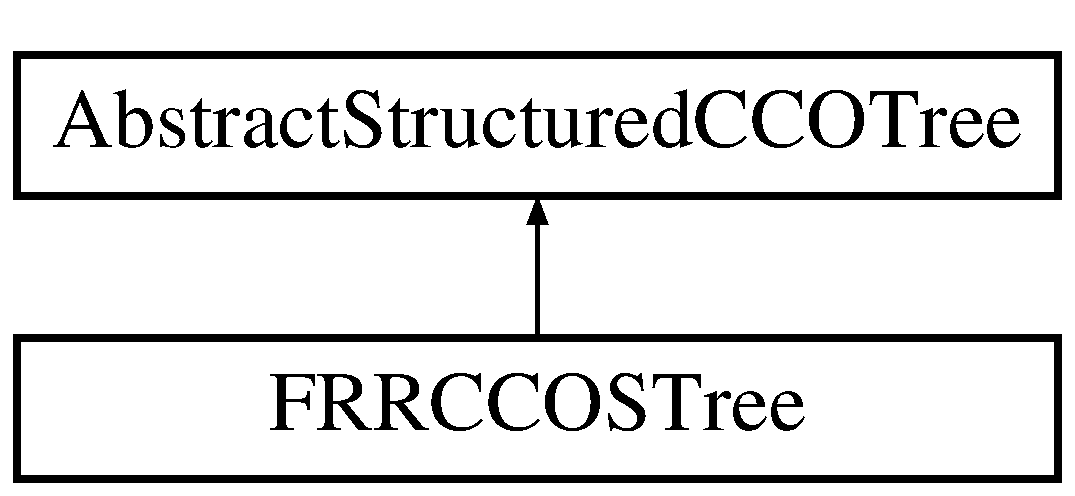
\includegraphics[height=2.000000cm]{db/d75/class_f_r_r_c_c_o_s_tree}
\end{center}
\end{figure}
\subsection*{Public Member Functions}
\begin{DoxyCompactItemize}
\item 
\hyperlink{class_f_r_r_c_c_o_s_tree_a522d48ce9c84769ff85366b9879881ec}{F\+R\+R\+C\+C\+O\+S\+Tree} (\hyperlink{structpoint}{point} xi, double \hyperlink{class_f_r_r_c_c_o_s_tree_a7cbf3091db38b3b573b84be820890bba}{root\+Radius}, double qi, \hyperlink{class_abstract_constraint_function}{Abstract\+Constraint\+Function}$<$ double, int $>$ $\ast$gam, \hyperlink{class_abstract_constraint_function}{Abstract\+Constraint\+Function}$<$ double, int $>$ $\ast$eps\+Lim, \hyperlink{class_abstract_constraint_function}{Abstract\+Constraint\+Function}$<$ double, int $>$ $\ast$nu, double min\+Angle, double ref\+Pressure, \hyperlink{class_generator_data}{Generator\+Data} $\ast$\hyperlink{class_abstract_structured_c_c_o_tree_af1836d7ed2156f3cf9cc311edfdc49b1}{instance\+Data})
\item 
\hyperlink{class_f_r_r_c_c_o_s_tree_a02bbf3ca159fe90abd0a48b9a6fc3ff3}{$\sim$\+F\+R\+R\+C\+C\+O\+S\+Tree} ()
\item 
\hyperlink{class_f_r_r_c_c_o_s_tree}{F\+R\+R\+C\+C\+O\+S\+Tree} $\ast$ \hyperlink{class_f_r_r_c_c_o_s_tree_a5c656f32e41e33023a2b92d82167efb4}{clone} ()
\item 
void \hyperlink{class_f_r_r_c_c_o_s_tree_a9114689c110d03da69c82bf2a833dcae}{get\+Closest\+Tree\+Point} (\hyperlink{structpoint}{point} x\+New, \hyperlink{structpoint}{point} $\ast$x\+Bif, double $\ast$dist)
\item 
vector$<$ \hyperlink{structvessel}{vessel} $\ast$ $>$ \hyperlink{class_f_r_r_c_c_o_s_tree_a51eeb636beadda63f0496ca3385c60f1}{get\+Close\+Segments} (\hyperlink{structpoint}{point} x\+New, \hyperlink{class_abstract_domain}{Abstract\+Domain} $\ast$domain, int $\ast$n\+Found)
\item 
void \hyperlink{class_f_r_r_c_c_o_s_tree_a91c2d539ccbd91c0f07a4366206e01da}{add\+Vessel} (\hyperlink{structpoint}{point} x\+Prox, \hyperlink{structpoint}{point} x\+Dist, \hyperlink{structvessel}{vessel} $\ast$parent)
\item 
int \hyperlink{class_f_r_r_c_c_o_s_tree_af1acf826014beab94a1a177b510cb7df}{test\+Vessel} (\hyperlink{structpoint}{point} x\+New, \hyperlink{structvessel}{vessel} $\ast$parent, \hyperlink{class_abstract_domain}{Abstract\+Domain} $\ast$domain, vector$<$ \hyperlink{structvessel}{vessel} $\ast$ $>$ neighbors, double dlim, \hyperlink{structpoint}{point} $\ast$x\+Bif, double $\ast$cost)
\item 
void \hyperlink{class_f_r_r_c_c_o_s_tree_ae7f3b98fda3d82961e976f908c746852}{print} ()
\item 
string \hyperlink{class_f_r_r_c_c_o_s_tree_a78ad923289d1747b82e5c52a1e79f1f4}{get\+Tree\+Name} ()
\item 
double \hyperlink{class_f_r_r_c_c_o_s_tree_a34f5b4c8888e2254a1f8931d0134874d}{get\+Root\+Radius} ()
\end{DoxyCompactItemize}
\subsection*{Protected Member Functions}
\begin{DoxyCompactItemize}
\item 
void \hyperlink{class_f_r_r_c_c_o_s_tree_abd03a4c2e3080ad725a5d7a8f7c66e79}{save\+Tree} (ofstream $\ast$out\+File)
\end{DoxyCompactItemize}
\subsection*{Private Member Functions}
\begin{DoxyCompactItemize}
\item 
\hyperlink{structvessel}{vessel} $\ast$ \hyperlink{class_f_r_r_c_c_o_s_tree_aef5d8d11c6a6c054a8bfd9d8f75542ef}{clone\+Tree} (\hyperlink{structvessel}{vessel} $\ast$root, vector$<$ \hyperlink{structvessel}{vessel} $\ast$ $>$ $\ast$segments)
\item 
double \hyperlink{class_f_r_r_c_c_o_s_tree_a2e14dce4de0c9a04fe659bf7ba09935d}{evaluate} (\hyperlink{structpoint}{point} x\+New, \hyperlink{structpoint}{point} x\+Test, \hyperlink{structvessel}{vessel} $\ast$parent)
\item 
void \hyperlink{class_f_r_r_c_c_o_s_tree_ac874d76d1061662b2893b62d491e65cb}{update\+Tree} (\hyperlink{structvessel}{vessel} $\ast$root, \hyperlink{class_f_r_r_c_c_o_s_tree}{F\+R\+R\+C\+C\+O\+S\+Tree} $\ast$tree)
\item 
int \hyperlink{class_f_r_r_c_c_o_s_tree_acf03af1cd54ab2359de1cbefc437db95}{is\+Symmetrically\+Valid} (double beta1, double beta2, int n\+Level)
\item 
int \hyperlink{class_f_r_r_c_c_o_s_tree_a94b12ec6e8a68179b9cd646ab49a3ed9}{are\+Valid\+Angles} (\hyperlink{structpoint}{point} x\+Bif, \hyperlink{structpoint}{point} x\+New, \hyperlink{structvessel}{vessel} $\ast$parent)
\item 
int \hyperlink{class_f_r_r_c_c_o_s_tree_a6826a8f9cc486d98b659509f21e911c2}{is\+Overlapped} (\hyperlink{structpoint}{point} x\+Bif, \hyperlink{structpoint}{point} x\+New, \hyperlink{structvessel}{vessel} $\ast$parent, double d\+Lim)
\item 
int \hyperlink{class_f_r_r_c_c_o_s_tree_a17370e9ea2a973df943ce220b3a799a1}{is\+Intersecting\+Vessels} (\hyperlink{structpoint}{point} p1, \hyperlink{structpoint}{point} p2, \hyperlink{structvessel}{vessel} $\ast$parent, vector$<$ \hyperlink{structvessel}{vessel} $\ast$ $>$ neighbors)
\end{DoxyCompactItemize}
\subsection*{Private Attributes}
\begin{DoxyCompactItemize}
\item 
double \hyperlink{class_f_r_r_c_c_o_s_tree_a7cbf3091db38b3b573b84be820890bba}{root\+Radius}
\end{DoxyCompactItemize}
\subsection*{Additional Inherited Members}


\subsection{Detailed Description}
Models a single C\+CO tree which contains the vessel\textquotesingle{}s data and connectivity. The implementation corresponds to the algorithm 3 of Queiroz Ph.\+D. Thesis. Current implementation is endowed with Open\+MP parallelism. Specifications\+:
\begin{DoxyItemize}
\item Fixed domain;
\item Given flow Q;
\item Given pressure gradient;
\item Given N terminals;
\item Constant/variable symmetry per tree level;
\item Constant/variable Murray coefficient per tree level;
\item Constant/variable viscosity per tree level. 
\end{DoxyItemize}

\subsection{Constructor \& Destructor Documentation}
\index{F\+R\+R\+C\+C\+O\+S\+Tree@{F\+R\+R\+C\+C\+O\+S\+Tree}!F\+R\+R\+C\+C\+O\+S\+Tree@{F\+R\+R\+C\+C\+O\+S\+Tree}}
\index{F\+R\+R\+C\+C\+O\+S\+Tree@{F\+R\+R\+C\+C\+O\+S\+Tree}!F\+R\+R\+C\+C\+O\+S\+Tree@{F\+R\+R\+C\+C\+O\+S\+Tree}}
\subsubsection[{\texorpdfstring{F\+R\+R\+C\+C\+O\+S\+Tree(point xi, double root\+Radius, double qi, Abstract\+Constraint\+Function$<$ double, int $>$ $\ast$gam, Abstract\+Constraint\+Function$<$ double, int $>$ $\ast$eps\+Lim, Abstract\+Constraint\+Function$<$ double, int $>$ $\ast$nu, double min\+Angle, double ref\+Pressure, Generator\+Data $\ast$instance\+Data)}{FRRCCOSTree(point xi, double rootRadius, double qi, AbstractConstraintFunction< double, int > *gam, AbstractConstraintFunction< double, int > *epsLim, AbstractConstraintFunction< double, int > *nu, double minAngle, double refPressure, GeneratorData *instanceData)}}]{\setlength{\rightskip}{0pt plus 5cm}F\+R\+R\+C\+C\+O\+S\+Tree\+::\+F\+R\+R\+C\+C\+O\+S\+Tree (
\begin{DoxyParamCaption}
\item[{{\bf point}}]{xi, }
\item[{double}]{root\+Radius, }
\item[{double}]{qi, }
\item[{{\bf Abstract\+Constraint\+Function}$<$ double, int $>$ $\ast$}]{gam, }
\item[{{\bf Abstract\+Constraint\+Function}$<$ double, int $>$ $\ast$}]{eps\+Lim, }
\item[{{\bf Abstract\+Constraint\+Function}$<$ double, int $>$ $\ast$}]{nu, }
\item[{double}]{min\+Angle, }
\item[{double}]{ref\+Pressure, }
\item[{{\bf Generator\+Data} $\ast$}]{instance\+Data}
\end{DoxyParamCaption}
)}\hypertarget{class_f_r_r_c_c_o_s_tree_a522d48ce9c84769ff85366b9879881ec}{}\label{class_f_r_r_c_c_o_s_tree_a522d48ce9c84769ff85366b9879881ec}
Common tree creator. 
\begin{DoxyParams}{Parameters}
{\em xi} & Root point. \\
\hline
{\em root\+Radius} & Root radius. \\
\hline
{\em qi} & Flow at the root. \\
\hline
{\em gam} & Murray law function. \\
\hline
{\em eps\+Lim} & Sibling vessels ratio function. \\
\hline
{\em nu} & Viscosity function with respect to the tree level. \\
\hline
{\em min\+Angle} & Minimum angle allowed. \\
\hline
\end{DoxyParams}
\index{F\+R\+R\+C\+C\+O\+S\+Tree@{F\+R\+R\+C\+C\+O\+S\+Tree}!````~F\+R\+R\+C\+C\+O\+S\+Tree@{$\sim$\+F\+R\+R\+C\+C\+O\+S\+Tree}}
\index{````~F\+R\+R\+C\+C\+O\+S\+Tree@{$\sim$\+F\+R\+R\+C\+C\+O\+S\+Tree}!F\+R\+R\+C\+C\+O\+S\+Tree@{F\+R\+R\+C\+C\+O\+S\+Tree}}
\subsubsection[{\texorpdfstring{$\sim$\+F\+R\+R\+C\+C\+O\+S\+Tree()}{~FRRCCOSTree()}}]{\setlength{\rightskip}{0pt plus 5cm}F\+R\+R\+C\+C\+O\+S\+Tree\+::$\sim$\+F\+R\+R\+C\+C\+O\+S\+Tree (
\begin{DoxyParamCaption}
{}
\end{DoxyParamCaption}
)}\hypertarget{class_f_r_r_c_c_o_s_tree_a02bbf3ca159fe90abd0a48b9a6fc3ff3}{}\label{class_f_r_r_c_c_o_s_tree_a02bbf3ca159fe90abd0a48b9a6fc3ff3}
Common destructor. 

\subsection{Member Function Documentation}
\index{F\+R\+R\+C\+C\+O\+S\+Tree@{F\+R\+R\+C\+C\+O\+S\+Tree}!add\+Vessel@{add\+Vessel}}
\index{add\+Vessel@{add\+Vessel}!F\+R\+R\+C\+C\+O\+S\+Tree@{F\+R\+R\+C\+C\+O\+S\+Tree}}
\subsubsection[{\texorpdfstring{add\+Vessel(point x\+Prox, point x\+Dist, vessel $\ast$parent)}{addVessel(point xProx, point xDist, vessel *parent)}}]{\setlength{\rightskip}{0pt plus 5cm}void F\+R\+R\+C\+C\+O\+S\+Tree\+::add\+Vessel (
\begin{DoxyParamCaption}
\item[{{\bf point}}]{x\+Prox, }
\item[{{\bf point}}]{x\+Dist, }
\item[{{\bf vessel} $\ast$}]{parent}
\end{DoxyParamCaption}
)\hspace{0.3cm}{\ttfamily [virtual]}}\hypertarget{class_f_r_r_c_c_o_s_tree_a91c2d539ccbd91c0f07a4366206e01da}{}\label{class_f_r_r_c_c_o_s_tree_a91c2d539ccbd91c0f07a4366206e01da}
Adds a new vessel to the C\+CO tree. 
\begin{DoxyParams}{Parameters}
{\em x\+Prox} & and \\
\hline
{\em x\+Dist} & are the proximal and distal nodes of the new vessel and \\
\hline
{\em parent} & is the attachment parent vessel. \\
\hline
{\em x\+Prox} & Proximal point of the new vessel. \\
\hline
{\em x\+Dist} & Distal point of the new vessel. \\
\hline
{\em parent} & Parent to the new vessel. \\
\hline
\end{DoxyParams}


Implements \hyperlink{class_abstract_structured_c_c_o_tree_af592741d1d89d62834e9d58a72cb40af}{Abstract\+Structured\+C\+C\+O\+Tree}.

\index{F\+R\+R\+C\+C\+O\+S\+Tree@{F\+R\+R\+C\+C\+O\+S\+Tree}!are\+Valid\+Angles@{are\+Valid\+Angles}}
\index{are\+Valid\+Angles@{are\+Valid\+Angles}!F\+R\+R\+C\+C\+O\+S\+Tree@{F\+R\+R\+C\+C\+O\+S\+Tree}}
\subsubsection[{\texorpdfstring{are\+Valid\+Angles(point x\+Bif, point x\+New, vessel $\ast$parent)}{areValidAngles(point xBif, point xNew, vessel *parent)}}]{\setlength{\rightskip}{0pt plus 5cm}int F\+R\+R\+C\+C\+O\+S\+Tree\+::are\+Valid\+Angles (
\begin{DoxyParamCaption}
\item[{{\bf point}}]{x\+Bif, }
\item[{{\bf point}}]{x\+New, }
\item[{{\bf vessel} $\ast$}]{parent}
\end{DoxyParamCaption}
)\hspace{0.3cm}{\ttfamily [private]}}\hypertarget{class_f_r_r_c_c_o_s_tree_a94b12ec6e8a68179b9cd646ab49a3ed9}{}\label{class_f_r_r_c_c_o_s_tree_a94b12ec6e8a68179b9cd646ab49a3ed9}
Checks if the angles of the parent vessel and the new vessel do not violate the minimum angle constraint. 
\begin{DoxyParams}{Parameters}
{\em x\+Bif} & Bifurcation point between the new vessel and the distal part of the parent vessel (i\+Con). \\
\hline
{\em x\+New} & Distal point of the new vessel. \\
\hline
{\em parent} & Parent vessel. \\
\hline
\end{DoxyParams}
\begin{DoxyReturn}{Returns}
If the angles are higher than the minimum allowed. 
\end{DoxyReturn}
\index{F\+R\+R\+C\+C\+O\+S\+Tree@{F\+R\+R\+C\+C\+O\+S\+Tree}!clone@{clone}}
\index{clone@{clone}!F\+R\+R\+C\+C\+O\+S\+Tree@{F\+R\+R\+C\+C\+O\+S\+Tree}}
\subsubsection[{\texorpdfstring{clone()}{clone()}}]{\setlength{\rightskip}{0pt plus 5cm}{\bf F\+R\+R\+C\+C\+O\+S\+Tree} $\ast$ F\+R\+R\+C\+C\+O\+S\+Tree\+::clone (
\begin{DoxyParamCaption}
{}
\end{DoxyParamCaption}
)}\hypertarget{class_f_r_r_c_c_o_s_tree_a5c656f32e41e33023a2b92d82167efb4}{}\label{class_f_r_r_c_c_o_s_tree_a5c656f32e41e33023a2b92d82167efb4}
Creates a copy from the tree without the vtk structures (neither from the tree nor from the vessels). \begin{DoxyReturn}{Returns}
Copy from the tree 
\end{DoxyReturn}
\index{F\+R\+R\+C\+C\+O\+S\+Tree@{F\+R\+R\+C\+C\+O\+S\+Tree}!clone\+Tree@{clone\+Tree}}
\index{clone\+Tree@{clone\+Tree}!F\+R\+R\+C\+C\+O\+S\+Tree@{F\+R\+R\+C\+C\+O\+S\+Tree}}
\subsubsection[{\texorpdfstring{clone\+Tree(vessel $\ast$root, vector$<$ vessel $\ast$ $>$ $\ast$segments)}{cloneTree(vessel *root, vector< vessel * > *segments)}}]{\setlength{\rightskip}{0pt plus 5cm}{\bf vessel} $\ast$ F\+R\+R\+C\+C\+O\+S\+Tree\+::clone\+Tree (
\begin{DoxyParamCaption}
\item[{{\bf vessel} $\ast$}]{root, }
\item[{vector$<$ {\bf vessel} $\ast$ $>$ $\ast$}]{segments}
\end{DoxyParamCaption}
)\hspace{0.3cm}{\ttfamily [private]}}\hypertarget{class_f_r_r_c_c_o_s_tree_aef5d8d11c6a6c054a8bfd9d8f75542ef}{}\label{class_f_r_r_c_c_o_s_tree_aef5d8d11c6a6c054a8bfd9d8f75542ef}
Clones the current tree. 
\begin{DoxyParams}{Parameters}
{\em root} & Root of the tree to clone. \\
\hline
{\em segments} & Segments of the tree. \\
\hline
\end{DoxyParams}
\begin{DoxyReturn}{Returns}
Cloned subtree. 
\end{DoxyReturn}
\index{F\+R\+R\+C\+C\+O\+S\+Tree@{F\+R\+R\+C\+C\+O\+S\+Tree}!evaluate@{evaluate}}
\index{evaluate@{evaluate}!F\+R\+R\+C\+C\+O\+S\+Tree@{F\+R\+R\+C\+C\+O\+S\+Tree}}
\subsubsection[{\texorpdfstring{evaluate(point x\+New, point x\+Test, vessel $\ast$parent)}{evaluate(point xNew, point xTest, vessel *parent)}}]{\setlength{\rightskip}{0pt plus 5cm}double F\+R\+R\+C\+C\+O\+S\+Tree\+::evaluate (
\begin{DoxyParamCaption}
\item[{{\bf point}}]{x\+New, }
\item[{{\bf point}}]{x\+Test, }
\item[{{\bf vessel} $\ast$}]{parent}
\end{DoxyParamCaption}
)\hspace{0.3cm}{\ttfamily [private]}}\hypertarget{class_f_r_r_c_c_o_s_tree_a2e14dce4de0c9a04fe659bf7ba09935d}{}\label{class_f_r_r_c_c_o_s_tree_a2e14dce4de0c9a04fe659bf7ba09935d}
Returns the updated functional cost due to the new segment inclusion. 
\begin{DoxyParams}{Parameters}
{\em x\+New} & Proximal point of the new vessel. \\
\hline
{\em x\+Test} & Distal point of the new vessel. \\
\hline
{\em parent} & Parent to the new vessel. \\
\hline
\end{DoxyParams}
\index{F\+R\+R\+C\+C\+O\+S\+Tree@{F\+R\+R\+C\+C\+O\+S\+Tree}!get\+Close\+Segments@{get\+Close\+Segments}}
\index{get\+Close\+Segments@{get\+Close\+Segments}!F\+R\+R\+C\+C\+O\+S\+Tree@{F\+R\+R\+C\+C\+O\+S\+Tree}}
\subsubsection[{\texorpdfstring{get\+Close\+Segments(point x\+New, Abstract\+Domain $\ast$domain, int $\ast$n\+Found)}{getCloseSegments(point xNew, AbstractDomain *domain, int *nFound)}}]{\setlength{\rightskip}{0pt plus 5cm}vector$<$ {\bf vessel} $\ast$ $>$ F\+R\+R\+C\+C\+O\+S\+Tree\+::get\+Close\+Segments (
\begin{DoxyParamCaption}
\item[{{\bf point}}]{x\+New, }
\item[{{\bf Abstract\+Domain} $\ast$}]{domain, }
\item[{int $\ast$}]{n\+Found}
\end{DoxyParamCaption}
)\hspace{0.3cm}{\ttfamily [virtual]}}\hypertarget{class_f_r_r_c_c_o_s_tree_a51eeb636beadda63f0496ca3385c60f1}{}\label{class_f_r_r_c_c_o_s_tree_a51eeb636beadda63f0496ca3385c60f1}
Return the segments in a close neighborhood of {\ttfamily x\+New}. The neighborhood is computed based on the perfusion volume indicated by {\ttfamily domain}. 
\begin{DoxyParams}{Parameters}
{\em x\+New} & Center point of the neighborhood of interest. \\
\hline
{\em domain} & Domain of the segments. \\
\hline
{\em n\+Found} & Amount of segments in the neighborhood. \\
\hline
\end{DoxyParams}
\begin{DoxyReturn}{Returns}
Array of segments in the neighborhood of {\ttfamily x\+New}. 
\end{DoxyReturn}


Implements \hyperlink{class_abstract_structured_c_c_o_tree_a0371a4c9a5e8ddfd8b0cc8d811d60f04}{Abstract\+Structured\+C\+C\+O\+Tree}.

\index{F\+R\+R\+C\+C\+O\+S\+Tree@{F\+R\+R\+C\+C\+O\+S\+Tree}!get\+Closest\+Tree\+Point@{get\+Closest\+Tree\+Point}}
\index{get\+Closest\+Tree\+Point@{get\+Closest\+Tree\+Point}!F\+R\+R\+C\+C\+O\+S\+Tree@{F\+R\+R\+C\+C\+O\+S\+Tree}}
\subsubsection[{\texorpdfstring{get\+Closest\+Tree\+Point(point x\+New, point $\ast$x\+Bif, double $\ast$dist)}{getClosestTreePoint(point xNew, point *xBif, double *dist)}}]{\setlength{\rightskip}{0pt plus 5cm}void F\+R\+R\+C\+C\+O\+S\+Tree\+::get\+Closest\+Tree\+Point (
\begin{DoxyParamCaption}
\item[{{\bf point}}]{x\+New, }
\item[{{\bf point} $\ast$}]{x\+Bif, }
\item[{double $\ast$}]{dist}
\end{DoxyParamCaption}
)\hspace{0.3cm}{\ttfamily [virtual]}}\hypertarget{class_f_r_r_c_c_o_s_tree_a9114689c110d03da69c82bf2a833dcae}{}\label{class_f_r_r_c_c_o_s_tree_a9114689c110d03da69c82bf2a833dcae}
Returns the closest point in the C\+C\+O\+Tree with respect to {\ttfamily x\+New} point. 
\begin{DoxyParams}{Parameters}
{\em x\+New} & Point from which the minimum distance is computed. \\
\hline
{\em x\+Bif} & Closest point in the tree to {\ttfamily x\+New}. \\
\hline
{\em dist} & Minimum distance between {\ttfamily x\+New} and the tree. \\
\hline
\end{DoxyParams}


Implements \hyperlink{class_abstract_structured_c_c_o_tree_a09cb70d5e23065273d87dd0c0434e1c5}{Abstract\+Structured\+C\+C\+O\+Tree}.

\index{F\+R\+R\+C\+C\+O\+S\+Tree@{F\+R\+R\+C\+C\+O\+S\+Tree}!get\+Root\+Radius@{get\+Root\+Radius}}
\index{get\+Root\+Radius@{get\+Root\+Radius}!F\+R\+R\+C\+C\+O\+S\+Tree@{F\+R\+R\+C\+C\+O\+S\+Tree}}
\subsubsection[{\texorpdfstring{get\+Root\+Radius()}{getRootRadius()}}]{\setlength{\rightskip}{0pt plus 5cm}double F\+R\+R\+C\+C\+O\+S\+Tree\+::get\+Root\+Radius (
\begin{DoxyParamCaption}
{}
\end{DoxyParamCaption}
)}\hypertarget{class_f_r_r_c_c_o_s_tree_a34f5b4c8888e2254a1f8931d0134874d}{}\label{class_f_r_r_c_c_o_s_tree_a34f5b4c8888e2254a1f8931d0134874d}
Returns the root radius. \begin{DoxyReturn}{Returns}
Root radius. 
\end{DoxyReturn}
\index{F\+R\+R\+C\+C\+O\+S\+Tree@{F\+R\+R\+C\+C\+O\+S\+Tree}!get\+Tree\+Name@{get\+Tree\+Name}}
\index{get\+Tree\+Name@{get\+Tree\+Name}!F\+R\+R\+C\+C\+O\+S\+Tree@{F\+R\+R\+C\+C\+O\+S\+Tree}}
\subsubsection[{\texorpdfstring{get\+Tree\+Name()}{getTreeName()}}]{\setlength{\rightskip}{0pt plus 5cm}string F\+R\+R\+C\+C\+O\+S\+Tree\+::get\+Tree\+Name (
\begin{DoxyParamCaption}
{}
\end{DoxyParamCaption}
)\hspace{0.3cm}{\ttfamily [virtual]}}\hypertarget{class_f_r_r_c_c_o_s_tree_a78ad923289d1747b82e5c52a1e79f1f4}{}\label{class_f_r_r_c_c_o_s_tree_a78ad923289d1747b82e5c52a1e79f1f4}
Returns the class name identifier. \begin{DoxyReturn}{Returns}
Class name. 
\end{DoxyReturn}


Implements \hyperlink{class_abstract_structured_c_c_o_tree_a32e56a263498bc04c3c552fc7de30554}{Abstract\+Structured\+C\+C\+O\+Tree}.

\index{F\+R\+R\+C\+C\+O\+S\+Tree@{F\+R\+R\+C\+C\+O\+S\+Tree}!is\+Intersecting\+Vessels@{is\+Intersecting\+Vessels}}
\index{is\+Intersecting\+Vessels@{is\+Intersecting\+Vessels}!F\+R\+R\+C\+C\+O\+S\+Tree@{F\+R\+R\+C\+C\+O\+S\+Tree}}
\subsubsection[{\texorpdfstring{is\+Intersecting\+Vessels(point p1, point p2, vessel $\ast$parent, vector$<$ vessel $\ast$ $>$ neighbors)}{isIntersectingVessels(point p1, point p2, vessel *parent, vector< vessel * > neighbors)}}]{\setlength{\rightskip}{0pt plus 5cm}int F\+R\+R\+C\+C\+O\+S\+Tree\+::is\+Intersecting\+Vessels (
\begin{DoxyParamCaption}
\item[{{\bf point}}]{p1, }
\item[{{\bf point}}]{p2, }
\item[{{\bf vessel} $\ast$}]{parent, }
\item[{vector$<$ {\bf vessel} $\ast$ $>$}]{neighbors}
\end{DoxyParamCaption}
)\hspace{0.3cm}{\ttfamily [private]}}\hypertarget{class_f_r_r_c_c_o_s_tree_a17370e9ea2a973df943ce220b3a799a1}{}\label{class_f_r_r_c_c_o_s_tree_a17370e9ea2a973df943ce220b3a799a1}
It returns if the segment 
\begin{DoxyParams}{Parameters}
{\em p1} & -\/ \\
\hline
{\em p2} & intersects any vessel of the tree beside parent. \\
\hline
{\em p1} & Extreme point 1 of the line. \\
\hline
{\em p2} & Extreme point 2 of the line. \\
\hline
{\em parent} & Vessel excluded from the checking. \\
\hline
{\em boundary\+Tol} & Factor of line contraction at the extremes to avoid false intersections due to contact with anastomose. \\
\hline
\end{DoxyParams}
\begin{DoxyReturn}{Returns}
If the segment intersects any segment of the tree. 
\end{DoxyReturn}
\index{F\+R\+R\+C\+C\+O\+S\+Tree@{F\+R\+R\+C\+C\+O\+S\+Tree}!is\+Overlapped@{is\+Overlapped}}
\index{is\+Overlapped@{is\+Overlapped}!F\+R\+R\+C\+C\+O\+S\+Tree@{F\+R\+R\+C\+C\+O\+S\+Tree}}
\subsubsection[{\texorpdfstring{is\+Overlapped(point x\+Bif, point x\+New, vessel $\ast$parent, double d\+Lim)}{isOverlapped(point xBif, point xNew, vessel *parent, double dLim)}}]{\setlength{\rightskip}{0pt plus 5cm}int F\+R\+R\+C\+C\+O\+S\+Tree\+::is\+Overlapped (
\begin{DoxyParamCaption}
\item[{{\bf point}}]{x\+Bif, }
\item[{{\bf point}}]{x\+New, }
\item[{{\bf vessel} $\ast$}]{parent, }
\item[{double}]{d\+Lim}
\end{DoxyParamCaption}
)\hspace{0.3cm}{\ttfamily [private]}}\hypertarget{class_f_r_r_c_c_o_s_tree_a6826a8f9cc486d98b659509f21e911c2}{}\label{class_f_r_r_c_c_o_s_tree_a6826a8f9cc486d98b659509f21e911c2}
Determines if the segment x\+Bif-\/x\+New is closer than d\+Lim to any other segment of the tree (without being its parent vessel). Not used. 
\begin{DoxyParams}{Parameters}
{\em x\+Bif} & Proximal point for the new segment. \\
\hline
{\em x\+New} & Distal point for the new segment. \\
\hline
{\em parent} & Parent vessel of the new segment. \\
\hline
{\em d\+Lim} & Perfusion volume for each terminal at the current state of the tree. \\
\hline
\end{DoxyParams}
\begin{DoxyReturn}{Returns}
If the middle point of the segment is sufficiently distant from the tree. 
\end{DoxyReturn}
\index{F\+R\+R\+C\+C\+O\+S\+Tree@{F\+R\+R\+C\+C\+O\+S\+Tree}!is\+Symmetrically\+Valid@{is\+Symmetrically\+Valid}}
\index{is\+Symmetrically\+Valid@{is\+Symmetrically\+Valid}!F\+R\+R\+C\+C\+O\+S\+Tree@{F\+R\+R\+C\+C\+O\+S\+Tree}}
\subsubsection[{\texorpdfstring{is\+Symmetrically\+Valid(double beta1, double beta2, int n\+Level)}{isSymmetricallyValid(double beta1, double beta2, int nLevel)}}]{\setlength{\rightskip}{0pt plus 5cm}int F\+R\+R\+C\+C\+O\+S\+Tree\+::is\+Symmetrically\+Valid (
\begin{DoxyParamCaption}
\item[{double}]{beta1, }
\item[{double}]{beta2, }
\item[{int}]{n\+Level}
\end{DoxyParamCaption}
)\hspace{0.3cm}{\ttfamily [private]}}\hypertarget{class_f_r_r_c_c_o_s_tree_acf03af1cd54ab2359de1cbefc437db95}{}\label{class_f_r_r_c_c_o_s_tree_acf03af1cd54ab2359de1cbefc437db95}
For a giving pair of beta between sibling of a parent vessel, it analyze the symmetry constrain given by eps\+Lim function.


\begin{DoxyParams}{Parameters}
{\em beta1} & Beta for the 1st sibling. \\
\hline
{\em beta2} & Beta for the 2nd sibling. \\
\hline
{\em n\+Level} & Tree level of the bifurcation. \\
\hline
\end{DoxyParams}
\begin{DoxyReturn}{Returns}
If the simmetry constrain is satisfied. 
\end{DoxyReturn}
\index{F\+R\+R\+C\+C\+O\+S\+Tree@{F\+R\+R\+C\+C\+O\+S\+Tree}!print@{print}}
\index{print@{print}!F\+R\+R\+C\+C\+O\+S\+Tree@{F\+R\+R\+C\+C\+O\+S\+Tree}}
\subsubsection[{\texorpdfstring{print()}{print()}}]{\setlength{\rightskip}{0pt plus 5cm}void F\+R\+R\+C\+C\+O\+S\+Tree\+::print (
\begin{DoxyParamCaption}
{}
\end{DoxyParamCaption}
)\hspace{0.3cm}{\ttfamily [virtual]}}\hypertarget{class_f_r_r_c_c_o_s_tree_ae7f3b98fda3d82961e976f908c746852}{}\label{class_f_r_r_c_c_o_s_tree_ae7f3b98fda3d82961e976f908c746852}
Prints the current tree node by node. 

Implements \hyperlink{class_abstract_structured_c_c_o_tree_ab28e036b4d82004ab4bafa964d7f7c97}{Abstract\+Structured\+C\+C\+O\+Tree}.

\index{F\+R\+R\+C\+C\+O\+S\+Tree@{F\+R\+R\+C\+C\+O\+S\+Tree}!save\+Tree@{save\+Tree}}
\index{save\+Tree@{save\+Tree}!F\+R\+R\+C\+C\+O\+S\+Tree@{F\+R\+R\+C\+C\+O\+S\+Tree}}
\subsubsection[{\texorpdfstring{save\+Tree(ofstream $\ast$out\+File)}{saveTree(ofstream *outFile)}}]{\setlength{\rightskip}{0pt plus 5cm}void F\+R\+R\+C\+C\+O\+S\+Tree\+::save\+Tree (
\begin{DoxyParamCaption}
\item[{ofstream $\ast$}]{out\+File}
\end{DoxyParamCaption}
)\hspace{0.3cm}{\ttfamily [protected]}, {\ttfamily [virtual]}}\hypertarget{class_f_r_r_c_c_o_s_tree_abd03a4c2e3080ad725a5d7a8f7c66e79}{}\label{class_f_r_r_c_c_o_s_tree_abd03a4c2e3080ad725a5d7a8f7c66e79}
Returns a string with the tree atributes to create the .cco file. 
\begin{DoxyParams}{Parameters}
{\em out\+File} & File writer for the .cco file. \\
\hline
\end{DoxyParams}


Reimplemented from \hyperlink{class_abstract_structured_c_c_o_tree_a16fb849f7fa74189c6b74c60ce59e776}{Abstract\+Structured\+C\+C\+O\+Tree}.

\index{F\+R\+R\+C\+C\+O\+S\+Tree@{F\+R\+R\+C\+C\+O\+S\+Tree}!test\+Vessel@{test\+Vessel}}
\index{test\+Vessel@{test\+Vessel}!F\+R\+R\+C\+C\+O\+S\+Tree@{F\+R\+R\+C\+C\+O\+S\+Tree}}
\subsubsection[{\texorpdfstring{test\+Vessel(point x\+New, vessel $\ast$parent, Abstract\+Domain $\ast$domain, vector$<$ vessel $\ast$ $>$ neighbors, double dlim, point $\ast$x\+Bif, double $\ast$cost)}{testVessel(point xNew, vessel *parent, AbstractDomain *domain, vector< vessel * > neighbors, double dlim, point *xBif, double *cost)}}]{\setlength{\rightskip}{0pt plus 5cm}int F\+R\+R\+C\+C\+O\+S\+Tree\+::test\+Vessel (
\begin{DoxyParamCaption}
\item[{{\bf point}}]{x\+New, }
\item[{{\bf vessel} $\ast$}]{parent, }
\item[{{\bf Abstract\+Domain} $\ast$}]{domain, }
\item[{vector$<$ {\bf vessel} $\ast$ $>$}]{neighbors, }
\item[{double}]{d\+Lim, }
\item[{{\bf point} $\ast$}]{x\+Bif, }
\item[{double $\ast$}]{cost}
\end{DoxyParamCaption}
)\hspace{0.3cm}{\ttfamily [virtual]}}\hypertarget{class_f_r_r_c_c_o_s_tree_af1acf826014beab94a1a177b510cb7df}{}\label{class_f_r_r_c_c_o_s_tree_af1acf826014beab94a1a177b510cb7df}
For a given spatial point {\ttfamily x\+New} test its connection with {\ttfamily parent} vessel. It must evaluate if the restrictions of geometry and symmetry are satisfied and also if it do not intersects with other vessel of this tree. It returns in {\ttfamily cost} the functional value with the inclusion of such vessel. 
\begin{DoxyParams}{Parameters}
{\em x\+New} & Distal point for the new vessel to test. \\
\hline
{\em parent} & Parent vessel to test the {\ttfamily x\+New} point connection. \\
\hline
{\em domain} & Tree domain. \\
\hline
{\em neighbors} & Close neighbors used for intersection test. \\
\hline
{\em dlim} & Not used in the current implementation. \\
\hline
{\em x\+Bif} & Proximal point for the new vessel that present the lower function cost. \\
\hline
{\em cost} & Functional cost variation for the best bifurcation position. \\
\hline
\end{DoxyParams}
\begin{DoxyReturn}{Returns}
If the connection of the tree with x\+New is possible. If not {\ttfamily cost} is I\+N\+F\+I\+N\+I\+TY.
\end{DoxyReturn}
Tests N\+\_\+\+B\+I\+F\+\_\+\+T\+R\+I\+ES $\ast$ (N\+\_\+\+B\+I\+F\+\_\+\+T\+R\+I\+E\+S+1)/2 -\/ 3 possible positions for the bifurcation site in the triangle delineated by the triplet (x\+New, parent-\/$>$x\+Prox, parent-\/$>$x\+Dist). It returns the bifurcation site x\+Bif which corresponds to the minimum cost in terms of volumetric area of the tree. If all bifurcations are invalid, cost will be D\+B\+L\+\_\+\+M\+AX. 

Implements \hyperlink{class_abstract_structured_c_c_o_tree_ac566ae7f8357ce1f61f624d87a9daf86}{Abstract\+Structured\+C\+C\+O\+Tree}.

\index{F\+R\+R\+C\+C\+O\+S\+Tree@{F\+R\+R\+C\+C\+O\+S\+Tree}!update\+Tree@{update\+Tree}}
\index{update\+Tree@{update\+Tree}!F\+R\+R\+C\+C\+O\+S\+Tree@{F\+R\+R\+C\+C\+O\+S\+Tree}}
\subsubsection[{\texorpdfstring{update\+Tree(vessel $\ast$root, F\+R\+R\+C\+C\+O\+S\+Tree $\ast$tree)}{updateTree(vessel *root, FRRCCOSTree *tree)}}]{\setlength{\rightskip}{0pt plus 5cm}void F\+R\+R\+C\+C\+O\+S\+Tree\+::update\+Tree (
\begin{DoxyParamCaption}
\item[{{\bf vessel} $\ast$}]{root, }
\item[{{\bf F\+R\+R\+C\+C\+O\+S\+Tree} $\ast$}]{tree}
\end{DoxyParamCaption}
)\hspace{0.3cm}{\ttfamily [private]}}\hypertarget{class_f_r_r_c_c_o_s_tree_ac874d76d1061662b2893b62d491e65cb}{}\label{class_f_r_r_c_c_o_s_tree_ac874d76d1061662b2893b62d491e65cb}
Updates the tree values for the current topology in only one tree \char`\"{}in order\char`\"{} swept (O(\+N)). As the recursion deepens, the level number is computed for each element. As the recursion is returning, it computes the flow and resistance for the current node and the radius ratio for its childs. 
\begin{DoxyParams}{Parameters}
{\em root} & Root vessel for the tree to update. \\
\hline
{\em tree} & Tree to update. \\
\hline
\end{DoxyParams}


\subsection{Member Data Documentation}
\index{F\+R\+R\+C\+C\+O\+S\+Tree@{F\+R\+R\+C\+C\+O\+S\+Tree}!root\+Radius@{root\+Radius}}
\index{root\+Radius@{root\+Radius}!F\+R\+R\+C\+C\+O\+S\+Tree@{F\+R\+R\+C\+C\+O\+S\+Tree}}
\subsubsection[{\texorpdfstring{root\+Radius}{rootRadius}}]{\setlength{\rightskip}{0pt plus 5cm}double F\+R\+R\+C\+C\+O\+S\+Tree\+::root\+Radius\hspace{0.3cm}{\ttfamily [private]}}\hypertarget{class_f_r_r_c_c_o_s_tree_a7cbf3091db38b3b573b84be820890bba}{}\label{class_f_r_r_c_c_o_s_tree_a7cbf3091db38b3b573b84be820890bba}
Root radius. 

The documentation for this class was generated from the following files\+:\begin{DoxyCompactItemize}
\item 
structures/tree/F\+R\+R\+C\+C\+O\+S\+Tree.\+h\item 
structures/tree/F\+R\+R\+C\+C\+O\+S\+Tree.\+cpp\end{DoxyCompactItemize}

\hypertarget{class_f_r_r_s_tree_generator}{}\section{F\+R\+R\+S\+Tree\+Generator Class Reference}
\label{class_f_r_r_s_tree_generator}\index{F\+R\+R\+S\+Tree\+Generator@{F\+R\+R\+S\+Tree\+Generator}}


{\ttfamily \#include $<$F\+R\+R\+S\+Tree\+Generator.\+h$>$}

Inheritance diagram for F\+R\+R\+S\+Tree\+Generator\+:\begin{figure}[H]
\begin{center}
\leavevmode
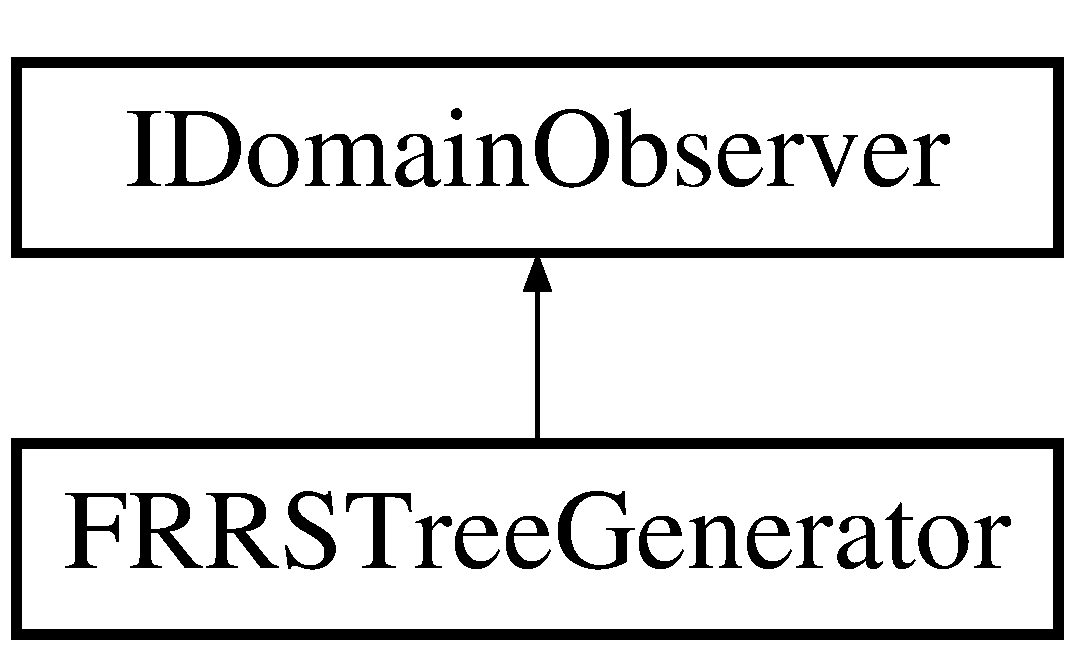
\includegraphics[height=2.000000cm]{d6/d46/class_f_r_r_s_tree_generator}
\end{center}
\end{figure}
\subsection*{Public Member Functions}
\begin{DoxyCompactItemize}
\item 
\hyperlink{class_f_r_r_s_tree_generator_a4089df88fb5f79d6484a300ea1e9f23e}{F\+R\+R\+S\+Tree\+Generator} (\hyperlink{class_abstract_domain}{Abstract\+Domain} $\ast$\hyperlink{class_f_r_r_s_tree_generator_a0322f396324a87545b29a7abce226ba6}{domain}, \hyperlink{structpoint}{point} xi, double root\+Radii, double qi, long long int n\+Term, \hyperlink{class_abstract_constraint_function}{Abstract\+Constraint\+Function}$<$ double, int $>$ $\ast$gam, \hyperlink{class_abstract_constraint_function}{Abstract\+Constraint\+Function}$<$ double, int $>$ $\ast$eps\+Lim, \hyperlink{class_abstract_constraint_function}{Abstract\+Constraint\+Function}$<$ double, int $>$ $\ast$nu, double min\+Angle, double ref\+Pressure)
\item 
\hyperlink{class_f_r_r_s_tree_generator_a147392a75aa6c3e6a51ee0fc56065064}{F\+R\+R\+S\+Tree\+Generator} (\hyperlink{class_abstract_domain}{Abstract\+Domain} $\ast$\hyperlink{class_f_r_r_s_tree_generator_a0322f396324a87545b29a7abce226ba6}{domain}, \hyperlink{structpoint}{point} xi, double root\+Radii, double qi, long long int n\+Term, \hyperlink{class_abstract_constraint_function}{Abstract\+Constraint\+Function}$<$ double, int $>$ $\ast$gam, \hyperlink{class_abstract_constraint_function}{Abstract\+Constraint\+Function}$<$ double, int $>$ $\ast$eps\+Lim, \hyperlink{class_abstract_constraint_function}{Abstract\+Constraint\+Function}$<$ double, int $>$ $\ast$nu, double min\+Angle, double ref\+Pressure, double viscosity\+Tolerance, int optimized)
\item 
\hyperlink{class_f_r_r_s_tree_generator_aa736ce95767783ce3a652e588ea3ffbd}{F\+R\+R\+S\+Tree\+Generator} (\hyperlink{class_abstract_domain}{Abstract\+Domain} $\ast$\hyperlink{class_f_r_r_s_tree_generator_a0322f396324a87545b29a7abce226ba6}{domain}, \hyperlink{class_abstract_structured_c_c_o_tree}{Abstract\+Structured\+C\+C\+O\+Tree} $\ast$\hyperlink{class_f_r_r_s_tree_generator_a9ff03e7c286d96e19d2fa658d167f519}{tree}, long long int n\+Term, \hyperlink{class_abstract_constraint_function}{Abstract\+Constraint\+Function}$<$ double, int $>$ $\ast$gam, \hyperlink{class_abstract_constraint_function}{Abstract\+Constraint\+Function}$<$ double, int $>$ $\ast$eps\+Lim, \hyperlink{class_abstract_constraint_function}{Abstract\+Constraint\+Function}$<$ double, int $>$ $\ast$nu)
\item 
\hyperlink{class_abstract_structured_c_c_o_tree}{Abstract\+Structured\+C\+C\+O\+Tree} $\ast$ \hyperlink{class_f_r_r_s_tree_generator_a71695ffb49be21c57db23e6b7ed2f4ae}{generate} ()
\item 
\hyperlink{class_abstract_structured_c_c_o_tree}{Abstract\+Structured\+C\+C\+O\+Tree} $\ast$ \hyperlink{class_f_r_r_s_tree_generator_a498307f5cb3df4f5309d779bfad1b28e}{resume} ()
\item 
\hyperlink{class_abstract_domain}{Abstract\+Domain} $\ast$ \hyperlink{class_f_r_r_s_tree_generator_aed57fb5d92cd7b2be51ab3ab743a8710}{get\+Domain} ()
\item 
vector$<$ \hyperlink{class_abstract_structured_c_c_o_tree}{Abstract\+Structured\+C\+C\+O\+Tree} $\ast$ $>$ \hyperlink{class_f_r_r_s_tree_generator_af1814afb75ece4844ca2f72b4c996982}{get\+Trees} ()
\item 
void \hyperlink{class_f_r_r_s_tree_generator_a2b3e562bed19939788a3e09f5255ca50}{enable\+Configuration\+File} (string filename)
\item 
void \hyperlink{class_f_r_r_s_tree_generator_a4cde56db66ba928599c0ce263246c61e}{observable\+Modified} (\hyperlink{class_i_domain_observable}{I\+Domain\+Observable} $\ast$observable\+Instance)
\end{DoxyCompactItemize}
\subsection*{Protected Member Functions}
\begin{DoxyCompactItemize}
\item 
int \hyperlink{class_f_r_r_s_tree_generator_a89b17a72238007d528969bac0660d82f}{is\+Valid\+Root\+Segment} (\hyperlink{structpoint}{point} x\+New, int i\+Try)
\item 
int \hyperlink{class_f_r_r_s_tree_generator_aa6d8355cbe2c7df48655d2b4613523fb}{is\+Valid\+Segment} (\hyperlink{structpoint}{point} x\+New, int i\+Try)
\item 
void \hyperlink{class_f_r_r_s_tree_generator_a1ecd8b31064344d19020732ca75e303f}{generates\+Configuration\+File} (ios\+::openmode mode)
\item 
void \hyperlink{class_f_r_r_s_tree_generator_affae083955045dfeafcd4bacc5d3a813}{mark\+Timestamp\+On\+Configuration\+File} (string label)
\item 
void \hyperlink{class_f_r_r_s_tree_generator_a2e27ffe1a6579085ed55de3a4a5d9251}{close\+Configuration\+File} ()
\end{DoxyCompactItemize}
\subsection*{Protected Attributes}
\begin{DoxyCompactItemize}
\item 
ofstream \hyperlink{class_f_r_r_s_tree_generator_abf91a61b2c3bfe74aa0d133796fc0aae}{conf\+File}
\item 
chrono\+::steady\+\_\+clock\+::time\+\_\+point \hyperlink{class_f_r_r_s_tree_generator_a3ee12afb75c0da076ff9f7a6a2755760}{beginning\+Time}
\end{DoxyCompactItemize}
\subsection*{Private Attributes}
\begin{DoxyCompactItemize}
\item 
\hyperlink{class_generator_data}{Generator\+Data} $\ast$ \hyperlink{class_f_r_r_s_tree_generator_a7e68f9ebd5171fbdc79d8ebac7ccc61c}{instance\+Data}
\item 
\hyperlink{class_generator_data_monitor}{Generator\+Data\+Monitor} $\ast$ \hyperlink{class_f_r_r_s_tree_generator_a8a6b326c69ca8feeee284ecdf741df00}{data\+Monitor}
\item 
long long int \hyperlink{class_f_r_r_s_tree_generator_a90d76e26de1b890e167ac570286b7615}{n\+Terminals}
\item 
double \hyperlink{class_f_r_r_s_tree_generator_afd3e174612083f26557c69374a4aabd9}{d\+Lim}
\item 
\hyperlink{class_abstract_domain}{Abstract\+Domain} $\ast$ \hyperlink{class_f_r_r_s_tree_generator_a0322f396324a87545b29a7abce226ba6}{domain}
\item 
\hyperlink{class_abstract_structured_c_c_o_tree}{Abstract\+Structured\+C\+C\+O\+Tree} $\ast$ \hyperlink{class_f_r_r_s_tree_generator_a9ff03e7c286d96e19d2fa658d167f519}{tree}
\item 
int \hyperlink{class_f_r_r_s_tree_generator_a6fc7001478ea0ce3c7ea4df930239221}{is\+Generating\+Conf\+File}
\item 
string \hyperlink{class_f_r_r_s_tree_generator_a5223ff3d634e30abe72a9156f364fce2}{conf\+Filename}
\end{DoxyCompactItemize}


\subsection{Detailed Description}
Generator for a single fixed perfusion tree. 

\subsection{Constructor \& Destructor Documentation}
\index{F\+R\+R\+S\+Tree\+Generator@{F\+R\+R\+S\+Tree\+Generator}!F\+R\+R\+S\+Tree\+Generator@{F\+R\+R\+S\+Tree\+Generator}}
\index{F\+R\+R\+S\+Tree\+Generator@{F\+R\+R\+S\+Tree\+Generator}!F\+R\+R\+S\+Tree\+Generator@{F\+R\+R\+S\+Tree\+Generator}}
\subsubsection[{\texorpdfstring{F\+R\+R\+S\+Tree\+Generator(\+Abstract\+Domain $\ast$domain, point xi, double root\+Radii, double qi, long long int n\+Term, Abstract\+Constraint\+Function$<$ double, int $>$ $\ast$gam, Abstract\+Constraint\+Function$<$ double, int $>$ $\ast$eps\+Lim, Abstract\+Constraint\+Function$<$ double, int $>$ $\ast$nu, double min\+Angle, double ref\+Pressure)}{FRRSTreeGenerator(AbstractDomain *domain, point xi, double rootRadii, double qi, long long int nTerm, AbstractConstraintFunction< double, int > *gam, AbstractConstraintFunction< double, int > *epsLim, AbstractConstraintFunction< double, int > *nu, double minAngle, double refPressure)}}]{\setlength{\rightskip}{0pt plus 5cm}F\+R\+R\+S\+Tree\+Generator\+::\+F\+R\+R\+S\+Tree\+Generator (
\begin{DoxyParamCaption}
\item[{{\bf Abstract\+Domain} $\ast$}]{domain, }
\item[{{\bf point}}]{xi, }
\item[{double}]{root\+Radii, }
\item[{double}]{qi, }
\item[{long long int}]{n\+Term, }
\item[{{\bf Abstract\+Constraint\+Function}$<$ double, int $>$ $\ast$}]{gam, }
\item[{{\bf Abstract\+Constraint\+Function}$<$ double, int $>$ $\ast$}]{eps\+Lim, }
\item[{{\bf Abstract\+Constraint\+Function}$<$ double, int $>$ $\ast$}]{nu, }
\item[{double}]{min\+Angle, }
\item[{double}]{ref\+Pressure}
\end{DoxyParamCaption}
)}\hypertarget{class_f_r_r_s_tree_generator_a4089df88fb5f79d6484a300ea1e9f23e}{}\label{class_f_r_r_s_tree_generator_a4089df88fb5f79d6484a300ea1e9f23e}
Constructor for non-\/optimized and constant viscosity tree. 
\begin{DoxyParams}{Parameters}
{\em domain} & Perfusion domain. \\
\hline
{\em xi} & Root proximal position. \\
\hline
{\em root\+Radii} & Root radius. \\
\hline
{\em qi} & Inflow for the perfusion domain. \\
\hline
{\em n\+Term} & Total number of tree terminals. \\
\hline
{\em gam} & Murray\textquotesingle{}s power law function. \\
\hline
{\em eps\+Lim} & Symmetry constraint function. \\
\hline
{\em nu} & Viscosity function. \\
\hline
{\em min\+Angle} & Minimum allowed bifurcation angle. \\
\hline
\end{DoxyParams}
\index{F\+R\+R\+S\+Tree\+Generator@{F\+R\+R\+S\+Tree\+Generator}!F\+R\+R\+S\+Tree\+Generator@{F\+R\+R\+S\+Tree\+Generator}}
\index{F\+R\+R\+S\+Tree\+Generator@{F\+R\+R\+S\+Tree\+Generator}!F\+R\+R\+S\+Tree\+Generator@{F\+R\+R\+S\+Tree\+Generator}}
\subsubsection[{\texorpdfstring{F\+R\+R\+S\+Tree\+Generator(\+Abstract\+Domain $\ast$domain, point xi, double root\+Radii, double qi, long long int n\+Term, Abstract\+Constraint\+Function$<$ double, int $>$ $\ast$gam, Abstract\+Constraint\+Function$<$ double, int $>$ $\ast$eps\+Lim, Abstract\+Constraint\+Function$<$ double, int $>$ $\ast$nu, double min\+Angle, double ref\+Pressure, double viscosity\+Tolerance, int optimized)}{FRRSTreeGenerator(AbstractDomain *domain, point xi, double rootRadii, double qi, long long int nTerm, AbstractConstraintFunction< double, int > *gam, AbstractConstraintFunction< double, int > *epsLim, AbstractConstraintFunction< double, int > *nu, double minAngle, double refPressure, double viscosityTolerance, int optimized)}}]{\setlength{\rightskip}{0pt plus 5cm}F\+R\+R\+S\+Tree\+Generator\+::\+F\+R\+R\+S\+Tree\+Generator (
\begin{DoxyParamCaption}
\item[{{\bf Abstract\+Domain} $\ast$}]{domain, }
\item[{{\bf point}}]{xi, }
\item[{double}]{root\+Radii, }
\item[{double}]{qi, }
\item[{long long int}]{n\+Term, }
\item[{{\bf Abstract\+Constraint\+Function}$<$ double, int $>$ $\ast$}]{gam, }
\item[{{\bf Abstract\+Constraint\+Function}$<$ double, int $>$ $\ast$}]{eps\+Lim, }
\item[{{\bf Abstract\+Constraint\+Function}$<$ double, int $>$ $\ast$}]{nu, }
\item[{double}]{min\+Angle, }
\item[{double}]{ref\+Pressure, }
\item[{double}]{viscosity\+Tolerance, }
\item[{int}]{optimized}
\end{DoxyParamCaption}
)}\hypertarget{class_f_r_r_s_tree_generator_a147392a75aa6c3e6a51ee0fc56065064}{}\label{class_f_r_r_s_tree_generator_a147392a75aa6c3e6a51ee0fc56065064}
Constructor for tree with Fahraeus-\/\+Lindquist viscosity model. 
\begin{DoxyParams}{Parameters}
{\em domain} & Perfusion domain. \\
\hline
{\em xi} & Root proximal position. \\
\hline
{\em root\+Radii} & Root radius. \\
\hline
{\em qi} & Inflow for the perfusion domain. \\
\hline
{\em n\+Term} & Total number of tree terminals. \\
\hline
{\em gam} & Murray\textquotesingle{}s power law function. \\
\hline
{\em eps\+Lim} & Symmetry constraint function. \\
\hline
{\em nu} & Viscosity function. \\
\hline
{\em min\+Angle} & Minimum allowed bifurcation angle. \\
\hline
{\em viscosity\+Tolerance} & Convergence tolerance for the absolute beta variation in the viscosity iterative scheme. \\
\hline
{\em optimized} & If it is optimized with partial tree scaling. \\
\hline
\end{DoxyParams}
\index{F\+R\+R\+S\+Tree\+Generator@{F\+R\+R\+S\+Tree\+Generator}!F\+R\+R\+S\+Tree\+Generator@{F\+R\+R\+S\+Tree\+Generator}}
\index{F\+R\+R\+S\+Tree\+Generator@{F\+R\+R\+S\+Tree\+Generator}!F\+R\+R\+S\+Tree\+Generator@{F\+R\+R\+S\+Tree\+Generator}}
\subsubsection[{\texorpdfstring{F\+R\+R\+S\+Tree\+Generator(\+Abstract\+Domain $\ast$domain, Abstract\+Structured\+C\+C\+O\+Tree $\ast$tree, long long int n\+Term, Abstract\+Constraint\+Function$<$ double, int $>$ $\ast$gam, Abstract\+Constraint\+Function$<$ double, int $>$ $\ast$eps\+Lim, Abstract\+Constraint\+Function$<$ double, int $>$ $\ast$nu)}{FRRSTreeGenerator(AbstractDomain *domain, AbstractStructuredCCOTree *tree, long long int nTerm, AbstractConstraintFunction< double, int > *gam, AbstractConstraintFunction< double, int > *epsLim, AbstractConstraintFunction< double, int > *nu)}}]{\setlength{\rightskip}{0pt plus 5cm}F\+R\+R\+S\+Tree\+Generator\+::\+F\+R\+R\+S\+Tree\+Generator (
\begin{DoxyParamCaption}
\item[{{\bf Abstract\+Domain} $\ast$}]{domain, }
\item[{{\bf Abstract\+Structured\+C\+C\+O\+Tree} $\ast$}]{tree, }
\item[{long long int}]{n\+Term, }
\item[{{\bf Abstract\+Constraint\+Function}$<$ double, int $>$ $\ast$}]{gam, }
\item[{{\bf Abstract\+Constraint\+Function}$<$ double, int $>$ $\ast$}]{eps\+Lim, }
\item[{{\bf Abstract\+Constraint\+Function}$<$ double, int $>$ $\ast$}]{nu}
\end{DoxyParamCaption}
)}\hypertarget{class_f_r_r_s_tree_generator_aa736ce95767783ce3a652e588ea3ffbd}{}\label{class_f_r_r_s_tree_generator_aa736ce95767783ce3a652e588ea3ffbd}
Constructor to resume from a pre-\/existent tree. 
\begin{DoxyParams}{Parameters}
{\em domain} & Perfusion domain. \\
\hline
{\em tree} & Pre-\/existent tree. \\
\hline
{\em n\+Term} & Total number of tree terminals. \\
\hline
{\em gam} & Murray\textquotesingle{}s power law function. \\
\hline
{\em eps\+Lim} & Symmetry constraint function. \\
\hline
{\em nu} & Viscosity function. \\
\hline
\end{DoxyParams}


\subsection{Member Function Documentation}
\index{F\+R\+R\+S\+Tree\+Generator@{F\+R\+R\+S\+Tree\+Generator}!close\+Configuration\+File@{close\+Configuration\+File}}
\index{close\+Configuration\+File@{close\+Configuration\+File}!F\+R\+R\+S\+Tree\+Generator@{F\+R\+R\+S\+Tree\+Generator}}
\subsubsection[{\texorpdfstring{close\+Configuration\+File()}{closeConfigurationFile()}}]{\setlength{\rightskip}{0pt plus 5cm}void F\+R\+R\+S\+Tree\+Generator\+::close\+Configuration\+File (
\begin{DoxyParamCaption}
{}
\end{DoxyParamCaption}
)\hspace{0.3cm}{\ttfamily [protected]}}\hypertarget{class_f_r_r_s_tree_generator_a2e27ffe1a6579085ed55de3a4a5d9251}{}\label{class_f_r_r_s_tree_generator_a2e27ffe1a6579085ed55de3a4a5d9251}
Closes the configuration file for the current tree generation. \index{F\+R\+R\+S\+Tree\+Generator@{F\+R\+R\+S\+Tree\+Generator}!enable\+Configuration\+File@{enable\+Configuration\+File}}
\index{enable\+Configuration\+File@{enable\+Configuration\+File}!F\+R\+R\+S\+Tree\+Generator@{F\+R\+R\+S\+Tree\+Generator}}
\subsubsection[{\texorpdfstring{enable\+Configuration\+File(string filename)}{enableConfigurationFile(string filename)}}]{\setlength{\rightskip}{0pt plus 5cm}void F\+R\+R\+S\+Tree\+Generator\+::enable\+Configuration\+File (
\begin{DoxyParamCaption}
\item[{string}]{filename}
\end{DoxyParamCaption}
)}\hypertarget{class_f_r_r_s_tree_generator_a2b3e562bed19939788a3e09f5255ca50}{}\label{class_f_r_r_s_tree_generator_a2b3e562bed19939788a3e09f5255ca50}
Enables the configuration file generation capabilities. 
\begin{DoxyParams}{Parameters}
{\em filename} & File name where the generator stores the configuration data. \\
\hline
\end{DoxyParams}
\index{F\+R\+R\+S\+Tree\+Generator@{F\+R\+R\+S\+Tree\+Generator}!generate@{generate}}
\index{generate@{generate}!F\+R\+R\+S\+Tree\+Generator@{F\+R\+R\+S\+Tree\+Generator}}
\subsubsection[{\texorpdfstring{generate()}{generate()}}]{\setlength{\rightskip}{0pt plus 5cm}{\bf Abstract\+Structured\+C\+C\+O\+Tree} $\ast$ F\+R\+R\+S\+Tree\+Generator\+::generate (
\begin{DoxyParamCaption}
{}
\end{DoxyParamCaption}
)}\hypertarget{class_f_r_r_s_tree_generator_a71695ffb49be21c57db23e6b7ed2f4ae}{}\label{class_f_r_r_s_tree_generator_a71695ffb49be21c57db23e6b7ed2f4ae}
Generates the specified tree. \begin{DoxyReturn}{Returns}
Perfusion tree. 
\end{DoxyReturn}
\index{F\+R\+R\+S\+Tree\+Generator@{F\+R\+R\+S\+Tree\+Generator}!generates\+Configuration\+File@{generates\+Configuration\+File}}
\index{generates\+Configuration\+File@{generates\+Configuration\+File}!F\+R\+R\+S\+Tree\+Generator@{F\+R\+R\+S\+Tree\+Generator}}
\subsubsection[{\texorpdfstring{generates\+Configuration\+File(ios\+::openmode mode)}{generatesConfigurationFile(ios::openmode mode)}}]{\setlength{\rightskip}{0pt plus 5cm}void F\+R\+R\+S\+Tree\+Generator\+::generates\+Configuration\+File (
\begin{DoxyParamCaption}
\item[{ios\+::openmode}]{mode}
\end{DoxyParamCaption}
)\hspace{0.3cm}{\ttfamily [protected]}}\hypertarget{class_f_r_r_s_tree_generator_a1ecd8b31064344d19020732ca75e303f}{}\label{class_f_r_r_s_tree_generator_a1ecd8b31064344d19020732ca75e303f}
Generates the configuration file for the current tree generation. 
\begin{DoxyParams}{Parameters}
{\em mode} & Is the openmode used for the generated file (ios\+::out for generation, ios\+::app for resume). \\
\hline
\end{DoxyParams}
\index{F\+R\+R\+S\+Tree\+Generator@{F\+R\+R\+S\+Tree\+Generator}!get\+Domain@{get\+Domain}}
\index{get\+Domain@{get\+Domain}!F\+R\+R\+S\+Tree\+Generator@{F\+R\+R\+S\+Tree\+Generator}}
\subsubsection[{\texorpdfstring{get\+Domain()}{getDomain()}}]{\setlength{\rightskip}{0pt plus 5cm}{\bf Abstract\+Domain} $\ast$ F\+R\+R\+S\+Tree\+Generator\+::get\+Domain (
\begin{DoxyParamCaption}
{}
\end{DoxyParamCaption}
)}\hypertarget{class_f_r_r_s_tree_generator_aed57fb5d92cd7b2be51ab3ab743a8710}{}\label{class_f_r_r_s_tree_generator_aed57fb5d92cd7b2be51ab3ab743a8710}
Returns the perfusion domain. \begin{DoxyReturn}{Returns}
Perfusion domain. 
\end{DoxyReturn}
\index{F\+R\+R\+S\+Tree\+Generator@{F\+R\+R\+S\+Tree\+Generator}!get\+Trees@{get\+Trees}}
\index{get\+Trees@{get\+Trees}!F\+R\+R\+S\+Tree\+Generator@{F\+R\+R\+S\+Tree\+Generator}}
\subsubsection[{\texorpdfstring{get\+Trees()}{getTrees()}}]{\setlength{\rightskip}{0pt plus 5cm}vector$<$ {\bf Abstract\+Structured\+C\+C\+O\+Tree} $\ast$ $>$ F\+R\+R\+S\+Tree\+Generator\+::get\+Trees (
\begin{DoxyParamCaption}
{}
\end{DoxyParamCaption}
)}\hypertarget{class_f_r_r_s_tree_generator_af1814afb75ece4844ca2f72b4c996982}{}\label{class_f_r_r_s_tree_generator_af1814afb75ece4844ca2f72b4c996982}
Returns the generated tree. \begin{DoxyReturn}{Returns}
Generated tree. 
\end{DoxyReturn}
\index{F\+R\+R\+S\+Tree\+Generator@{F\+R\+R\+S\+Tree\+Generator}!is\+Valid\+Root\+Segment@{is\+Valid\+Root\+Segment}}
\index{is\+Valid\+Root\+Segment@{is\+Valid\+Root\+Segment}!F\+R\+R\+S\+Tree\+Generator@{F\+R\+R\+S\+Tree\+Generator}}
\subsubsection[{\texorpdfstring{is\+Valid\+Root\+Segment(point x\+New, int i\+Try)}{isValidRootSegment(point xNew, int iTry)}}]{\setlength{\rightskip}{0pt plus 5cm}int F\+R\+R\+S\+Tree\+Generator\+::is\+Valid\+Root\+Segment (
\begin{DoxyParamCaption}
\item[{{\bf point}}]{x\+New, }
\item[{int}]{i\+Try}
\end{DoxyParamCaption}
)\hspace{0.3cm}{\ttfamily [protected]}}\hypertarget{class_f_r_r_s_tree_generator_a89b17a72238007d528969bac0660d82f}{}\label{class_f_r_r_s_tree_generator_a89b17a72238007d528969bac0660d82f}
Returns if the length of the segment defined by x\+Prox and x\+New is higher than d\+Lim (distance criterion). 
\begin{DoxyParams}{Parameters}
{\em x\+New} & Proposed distal point. \\
\hline
{\em i\+Try} & Number of trial. \\
\hline
\end{DoxyParams}
\begin{DoxyReturn}{Returns}
If the root segment is valid. 
\end{DoxyReturn}
\index{F\+R\+R\+S\+Tree\+Generator@{F\+R\+R\+S\+Tree\+Generator}!is\+Valid\+Segment@{is\+Valid\+Segment}}
\index{is\+Valid\+Segment@{is\+Valid\+Segment}!F\+R\+R\+S\+Tree\+Generator@{F\+R\+R\+S\+Tree\+Generator}}
\subsubsection[{\texorpdfstring{is\+Valid\+Segment(point x\+New, int i\+Try)}{isValidSegment(point xNew, int iTry)}}]{\setlength{\rightskip}{0pt plus 5cm}int F\+R\+R\+S\+Tree\+Generator\+::is\+Valid\+Segment (
\begin{DoxyParamCaption}
\item[{{\bf point}}]{x\+New, }
\item[{int}]{i\+Try}
\end{DoxyParamCaption}
)\hspace{0.3cm}{\ttfamily [protected]}}\hypertarget{class_f_r_r_s_tree_generator_aa6d8355cbe2c7df48655d2b4613523fb}{}\label{class_f_r_r_s_tree_generator_aa6d8355cbe2c7df48655d2b4613523fb}
Returns if the closest point to the whole try is greater than d\+Lim (distance criterion for a new segment). 
\begin{DoxyParams}{Parameters}
{\em x\+New} & Proposed distal point. \\
\hline
{\em i\+Try} & Number of trial. \\
\hline
\end{DoxyParams}
\begin{DoxyReturn}{Returns}
If the segment is valid. 
\end{DoxyReturn}
\index{F\+R\+R\+S\+Tree\+Generator@{F\+R\+R\+S\+Tree\+Generator}!mark\+Timestamp\+On\+Configuration\+File@{mark\+Timestamp\+On\+Configuration\+File}}
\index{mark\+Timestamp\+On\+Configuration\+File@{mark\+Timestamp\+On\+Configuration\+File}!F\+R\+R\+S\+Tree\+Generator@{F\+R\+R\+S\+Tree\+Generator}}
\subsubsection[{\texorpdfstring{mark\+Timestamp\+On\+Configuration\+File(string label)}{markTimestampOnConfigurationFile(string label)}}]{\setlength{\rightskip}{0pt plus 5cm}void F\+R\+R\+S\+Tree\+Generator\+::mark\+Timestamp\+On\+Configuration\+File (
\begin{DoxyParamCaption}
\item[{string}]{label}
\end{DoxyParamCaption}
)\hspace{0.3cm}{\ttfamily [protected]}}\hypertarget{class_f_r_r_s_tree_generator_affae083955045dfeafcd4bacc5d3a813}{}\label{class_f_r_r_s_tree_generator_affae083955045dfeafcd4bacc5d3a813}
Saves the timestamp for event {\ttfamily label}. \index{F\+R\+R\+S\+Tree\+Generator@{F\+R\+R\+S\+Tree\+Generator}!observable\+Modified@{observable\+Modified}}
\index{observable\+Modified@{observable\+Modified}!F\+R\+R\+S\+Tree\+Generator@{F\+R\+R\+S\+Tree\+Generator}}
\subsubsection[{\texorpdfstring{observable\+Modified(\+I\+Domain\+Observable $\ast$observable\+Instance)}{observableModified(IDomainObservable *observableInstance)}}]{\setlength{\rightskip}{0pt plus 5cm}void F\+R\+R\+S\+Tree\+Generator\+::observable\+Modified (
\begin{DoxyParamCaption}
\item[{{\bf I\+Domain\+Observable} $\ast$}]{observable\+Instance}
\end{DoxyParamCaption}
)\hspace{0.3cm}{\ttfamily [virtual]}}\hypertarget{class_f_r_r_s_tree_generator_a4cde56db66ba928599c0ce263246c61e}{}\label{class_f_r_r_s_tree_generator_a4cde56db66ba928599c0ce263246c61e}
Updates internal data from this instance after the domain has been modified. 
\begin{DoxyParams}{Parameters}
{\em observable\+Instance} & Domain instance modified. \\
\hline
\end{DoxyParams}


Implements \hyperlink{class_i_domain_observer_aee18640c20a6feaa16e4bf3bdde887a3}{I\+Domain\+Observer}.

\index{F\+R\+R\+S\+Tree\+Generator@{F\+R\+R\+S\+Tree\+Generator}!resume@{resume}}
\index{resume@{resume}!F\+R\+R\+S\+Tree\+Generator@{F\+R\+R\+S\+Tree\+Generator}}
\subsubsection[{\texorpdfstring{resume()}{resume()}}]{\setlength{\rightskip}{0pt plus 5cm}{\bf Abstract\+Structured\+C\+C\+O\+Tree} $\ast$ F\+R\+R\+S\+Tree\+Generator\+::resume (
\begin{DoxyParamCaption}
{}
\end{DoxyParamCaption}
)}\hypertarget{class_f_r_r_s_tree_generator_a498307f5cb3df4f5309d779bfad1b28e}{}\label{class_f_r_r_s_tree_generator_a498307f5cb3df4f5309d779bfad1b28e}
Resumes the tree generation. \begin{DoxyReturn}{Returns}
Perfusion tree. 
\end{DoxyReturn}


\subsection{Member Data Documentation}
\index{F\+R\+R\+S\+Tree\+Generator@{F\+R\+R\+S\+Tree\+Generator}!beginning\+Time@{beginning\+Time}}
\index{beginning\+Time@{beginning\+Time}!F\+R\+R\+S\+Tree\+Generator@{F\+R\+R\+S\+Tree\+Generator}}
\subsubsection[{\texorpdfstring{beginning\+Time}{beginningTime}}]{\setlength{\rightskip}{0pt plus 5cm}chrono\+::steady\+\_\+clock\+::time\+\_\+point F\+R\+R\+S\+Tree\+Generator\+::beginning\+Time\hspace{0.3cm}{\ttfamily [protected]}}\hypertarget{class_f_r_r_s_tree_generator_a3ee12afb75c0da076ff9f7a6a2755760}{}\label{class_f_r_r_s_tree_generator_a3ee12afb75c0da076ff9f7a6a2755760}
Initial timestamp of the generation process. \index{F\+R\+R\+S\+Tree\+Generator@{F\+R\+R\+S\+Tree\+Generator}!conf\+File@{conf\+File}}
\index{conf\+File@{conf\+File}!F\+R\+R\+S\+Tree\+Generator@{F\+R\+R\+S\+Tree\+Generator}}
\subsubsection[{\texorpdfstring{conf\+File}{confFile}}]{\setlength{\rightskip}{0pt plus 5cm}ofstream F\+R\+R\+S\+Tree\+Generator\+::conf\+File\hspace{0.3cm}{\ttfamily [protected]}}\hypertarget{class_f_r_r_s_tree_generator_abf91a61b2c3bfe74aa0d133796fc0aae}{}\label{class_f_r_r_s_tree_generator_abf91a61b2c3bfe74aa0d133796fc0aae}
Configuration file stream. \index{F\+R\+R\+S\+Tree\+Generator@{F\+R\+R\+S\+Tree\+Generator}!conf\+Filename@{conf\+Filename}}
\index{conf\+Filename@{conf\+Filename}!F\+R\+R\+S\+Tree\+Generator@{F\+R\+R\+S\+Tree\+Generator}}
\subsubsection[{\texorpdfstring{conf\+Filename}{confFilename}}]{\setlength{\rightskip}{0pt plus 5cm}string F\+R\+R\+S\+Tree\+Generator\+::conf\+Filename\hspace{0.3cm}{\ttfamily [private]}}\hypertarget{class_f_r_r_s_tree_generator_a5223ff3d634e30abe72a9156f364fce2}{}\label{class_f_r_r_s_tree_generator_a5223ff3d634e30abe72a9156f364fce2}
File name for the configuration file. \index{F\+R\+R\+S\+Tree\+Generator@{F\+R\+R\+S\+Tree\+Generator}!data\+Monitor@{data\+Monitor}}
\index{data\+Monitor@{data\+Monitor}!F\+R\+R\+S\+Tree\+Generator@{F\+R\+R\+S\+Tree\+Generator}}
\subsubsection[{\texorpdfstring{data\+Monitor}{dataMonitor}}]{\setlength{\rightskip}{0pt plus 5cm}{\bf Generator\+Data\+Monitor}$\ast$ F\+R\+R\+S\+Tree\+Generator\+::data\+Monitor\hspace{0.3cm}{\ttfamily [private]}}\hypertarget{class_f_r_r_s_tree_generator_a8a6b326c69ca8feeee284ecdf741df00}{}\label{class_f_r_r_s_tree_generator_a8a6b326c69ca8feeee284ecdf741df00}
Monitor of the {\ttfamily instance\+Data} . \index{F\+R\+R\+S\+Tree\+Generator@{F\+R\+R\+S\+Tree\+Generator}!d\+Lim@{d\+Lim}}
\index{d\+Lim@{d\+Lim}!F\+R\+R\+S\+Tree\+Generator@{F\+R\+R\+S\+Tree\+Generator}}
\subsubsection[{\texorpdfstring{d\+Lim}{dLim}}]{\setlength{\rightskip}{0pt plus 5cm}double F\+R\+R\+S\+Tree\+Generator\+::d\+Lim\hspace{0.3cm}{\ttfamily [private]}}\hypertarget{class_f_r_r_s_tree_generator_afd3e174612083f26557c69374a4aabd9}{}\label{class_f_r_r_s_tree_generator_afd3e174612083f26557c69374a4aabd9}
Perfusion volume. \index{F\+R\+R\+S\+Tree\+Generator@{F\+R\+R\+S\+Tree\+Generator}!domain@{domain}}
\index{domain@{domain}!F\+R\+R\+S\+Tree\+Generator@{F\+R\+R\+S\+Tree\+Generator}}
\subsubsection[{\texorpdfstring{domain}{domain}}]{\setlength{\rightskip}{0pt plus 5cm}{\bf Abstract\+Domain}$\ast$ F\+R\+R\+S\+Tree\+Generator\+::domain\hspace{0.3cm}{\ttfamily [private]}}\hypertarget{class_f_r_r_s_tree_generator_a0322f396324a87545b29a7abce226ba6}{}\label{class_f_r_r_s_tree_generator_a0322f396324a87545b29a7abce226ba6}
Perfusion domain. \index{F\+R\+R\+S\+Tree\+Generator@{F\+R\+R\+S\+Tree\+Generator}!instance\+Data@{instance\+Data}}
\index{instance\+Data@{instance\+Data}!F\+R\+R\+S\+Tree\+Generator@{F\+R\+R\+S\+Tree\+Generator}}
\subsubsection[{\texorpdfstring{instance\+Data}{instanceData}}]{\setlength{\rightskip}{0pt plus 5cm}{\bf Generator\+Data}$\ast$ F\+R\+R\+S\+Tree\+Generator\+::instance\+Data\hspace{0.3cm}{\ttfamily [private]}}\hypertarget{class_f_r_r_s_tree_generator_a7e68f9ebd5171fbdc79d8ebac7ccc61c}{}\label{class_f_r_r_s_tree_generator_a7e68f9ebd5171fbdc79d8ebac7ccc61c}
Wrapper with parameters associated to a tree generation process. \index{F\+R\+R\+S\+Tree\+Generator@{F\+R\+R\+S\+Tree\+Generator}!is\+Generating\+Conf\+File@{is\+Generating\+Conf\+File}}
\index{is\+Generating\+Conf\+File@{is\+Generating\+Conf\+File}!F\+R\+R\+S\+Tree\+Generator@{F\+R\+R\+S\+Tree\+Generator}}
\subsubsection[{\texorpdfstring{is\+Generating\+Conf\+File}{isGeneratingConfFile}}]{\setlength{\rightskip}{0pt plus 5cm}int F\+R\+R\+S\+Tree\+Generator\+::is\+Generating\+Conf\+File\hspace{0.3cm}{\ttfamily [private]}}\hypertarget{class_f_r_r_s_tree_generator_a6fc7001478ea0ce3c7ea4df930239221}{}\label{class_f_r_r_s_tree_generator_a6fc7001478ea0ce3c7ea4df930239221}
If the current generation saves the configuration used. \index{F\+R\+R\+S\+Tree\+Generator@{F\+R\+R\+S\+Tree\+Generator}!n\+Terminals@{n\+Terminals}}
\index{n\+Terminals@{n\+Terminals}!F\+R\+R\+S\+Tree\+Generator@{F\+R\+R\+S\+Tree\+Generator}}
\subsubsection[{\texorpdfstring{n\+Terminals}{nTerminals}}]{\setlength{\rightskip}{0pt plus 5cm}long long int F\+R\+R\+S\+Tree\+Generator\+::n\+Terminals\hspace{0.3cm}{\ttfamily [private]}}\hypertarget{class_f_r_r_s_tree_generator_a90d76e26de1b890e167ac570286b7615}{}\label{class_f_r_r_s_tree_generator_a90d76e26de1b890e167ac570286b7615}
Amount of terminals in the trees. \index{F\+R\+R\+S\+Tree\+Generator@{F\+R\+R\+S\+Tree\+Generator}!tree@{tree}}
\index{tree@{tree}!F\+R\+R\+S\+Tree\+Generator@{F\+R\+R\+S\+Tree\+Generator}}
\subsubsection[{\texorpdfstring{tree}{tree}}]{\setlength{\rightskip}{0pt plus 5cm}{\bf Abstract\+Structured\+C\+C\+O\+Tree}$\ast$ F\+R\+R\+S\+Tree\+Generator\+::tree\hspace{0.3cm}{\ttfamily [private]}}\hypertarget{class_f_r_r_s_tree_generator_a9ff03e7c286d96e19d2fa658d167f519}{}\label{class_f_r_r_s_tree_generator_a9ff03e7c286d96e19d2fa658d167f519}
Generated trees. 

The documentation for this class was generated from the following files\+:\begin{DoxyCompactItemize}
\item 
core/F\+R\+R\+S\+Tree\+Generator.\+h\item 
core/F\+R\+R\+S\+Tree\+Generator.\+cpp\end{DoxyCompactItemize}

\hypertarget{class_f_r_r_variable_viscosity_c_c_o_s_tree}{}\section{F\+R\+R\+Variable\+Viscosity\+C\+C\+O\+S\+Tree Class Reference}
\label{class_f_r_r_variable_viscosity_c_c_o_s_tree}\index{F\+R\+R\+Variable\+Viscosity\+C\+C\+O\+S\+Tree@{F\+R\+R\+Variable\+Viscosity\+C\+C\+O\+S\+Tree}}


{\ttfamily \#include $<$F\+R\+R\+Variable\+Viscosity\+C\+C\+O\+S\+Tree.\+h$>$}

Inheritance diagram for F\+R\+R\+Variable\+Viscosity\+C\+C\+O\+S\+Tree\+:\begin{figure}[H]
\begin{center}
\leavevmode
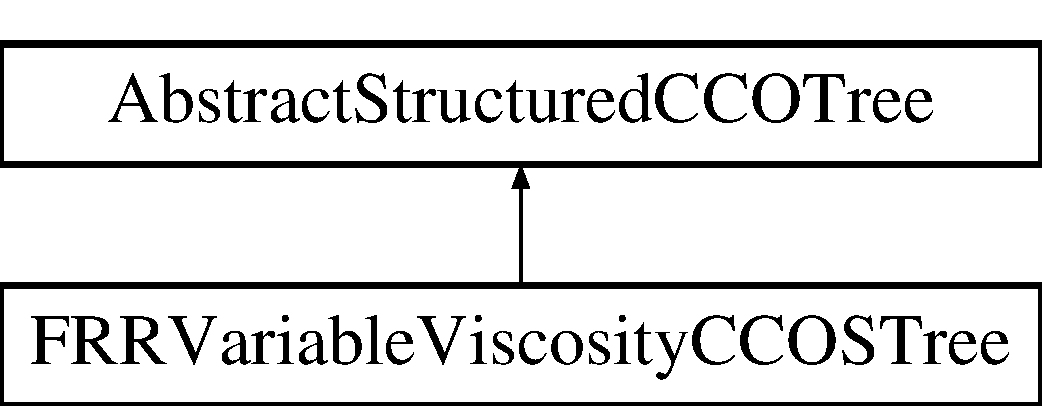
\includegraphics[height=2.000000cm]{da/df3/class_f_r_r_variable_viscosity_c_c_o_s_tree}
\end{center}
\end{figure}
\subsection*{Public Member Functions}
\begin{DoxyCompactItemize}
\item 
\hyperlink{class_f_r_r_variable_viscosity_c_c_o_s_tree_a112b1f39ea3592953d942d543f0b01fc}{F\+R\+R\+Variable\+Viscosity\+C\+C\+O\+S\+Tree} (\hyperlink{structpoint}{point} xi, double \hyperlink{class_f_r_r_variable_viscosity_c_c_o_s_tree_a15338c59c6dbecaeaeab80577a22c877}{root\+Radius}, double qi, \hyperlink{class_abstract_constraint_function}{Abstract\+Constraint\+Function}$<$ double, int $>$ $\ast$gam, \hyperlink{class_abstract_constraint_function}{Abstract\+Constraint\+Function}$<$ double, int $>$ $\ast$eps\+Lim, \hyperlink{class_abstract_constraint_function}{Abstract\+Constraint\+Function}$<$ double, int $>$ $\ast$nu, double min\+Angle, double ref\+Pressure, double resistance\+Variation\+Tolerance, \hyperlink{class_generator_data}{Generator\+Data} $\ast$\hyperlink{class_abstract_structured_c_c_o_tree_af1836d7ed2156f3cf9cc311edfdc49b1}{instance\+Data})
\item 
\hyperlink{class_f_r_r_variable_viscosity_c_c_o_s_tree_a2a51aa3ff3987afce48759ea27f2fa28}{$\sim$\+F\+R\+R\+Variable\+Viscosity\+C\+C\+O\+S\+Tree} ()
\item 
\hyperlink{class_f_r_r_variable_viscosity_c_c_o_s_tree}{F\+R\+R\+Variable\+Viscosity\+C\+C\+O\+S\+Tree} $\ast$ \hyperlink{class_f_r_r_variable_viscosity_c_c_o_s_tree_ab443fe67f0da340099405a8bdb42dfb6}{clone} ()
\item 
void \hyperlink{class_f_r_r_variable_viscosity_c_c_o_s_tree_a224c64cbf18976f660a730c5af0b73a0}{get\+Closest\+Tree\+Point} (\hyperlink{structpoint}{point} x\+New, \hyperlink{structpoint}{point} $\ast$x\+Bif, double $\ast$dist)
\item 
vector$<$ \hyperlink{structvessel}{vessel} $\ast$ $>$ \hyperlink{class_f_r_r_variable_viscosity_c_c_o_s_tree_a41e4e3406e5f78d50d5e597bad4950cd}{get\+Close\+Segments} (\hyperlink{structpoint}{point} x\+New, \hyperlink{class_abstract_domain}{Abstract\+Domain} $\ast$domain, int $\ast$n\+Found)
\item 
void \hyperlink{class_f_r_r_variable_viscosity_c_c_o_s_tree_a494a10a964337b83827012bfc03af194}{add\+Vessel} (\hyperlink{structpoint}{point} x\+Prox, \hyperlink{structpoint}{point} x\+Dist, \hyperlink{structvessel}{vessel} $\ast$parent)
\item 
int \hyperlink{class_f_r_r_variable_viscosity_c_c_o_s_tree_a339a5849edafcc7d315472a3fbed7987}{test\+Vessel} (\hyperlink{structpoint}{point} x\+New, \hyperlink{structvessel}{vessel} $\ast$parent, \hyperlink{class_abstract_domain}{Abstract\+Domain} $\ast$domain, vector$<$ \hyperlink{structvessel}{vessel} $\ast$ $>$ neighbors, double dlim, \hyperlink{structpoint}{point} $\ast$x\+Bif, double $\ast$cost)
\item 
void \hyperlink{class_f_r_r_variable_viscosity_c_c_o_s_tree_aec99594cf57192d80753147314483bc8}{print} ()
\item 
void \hyperlink{class_f_r_r_variable_viscosity_c_c_o_s_tree_abaa13c9055261bef97b112898e6106a2}{store\+V\+TK} (string filename)
\item 
string \hyperlink{class_f_r_r_variable_viscosity_c_c_o_s_tree_aac408960939d867d0a2014f4ced90d4d}{get\+Tree\+Name} ()
\item 
double \hyperlink{class_f_r_r_variable_viscosity_c_c_o_s_tree_a13cac292b851708de4900320582b4b14}{get\+Root\+Radius} ()
\end{DoxyCompactItemize}
\subsection*{Protected Member Functions}
\begin{DoxyCompactItemize}
\item 
void \hyperlink{class_f_r_r_variable_viscosity_c_c_o_s_tree_a545594bd2399bce109673929a46353ae}{save\+Tree} (ofstream $\ast$out\+File)
\end{DoxyCompactItemize}
\subsection*{Private Member Functions}
\begin{DoxyCompactItemize}
\item 
\hyperlink{structvessel}{vessel} $\ast$ \hyperlink{class_f_r_r_variable_viscosity_c_c_o_s_tree_ad3e31410f4bedfed9583ec2a4327a6f0}{clone\+Tree} (\hyperlink{structvessel}{vessel} $\ast$root, vector$<$ \hyperlink{structvessel}{vessel} $\ast$ $>$ $\ast$segments)
\item 
double \hyperlink{class_f_r_r_variable_viscosity_c_c_o_s_tree_aeb393ac0c5c6f613cdb74d2ebf810fd5}{evaluate} (\hyperlink{structpoint}{point} x\+New, \hyperlink{structpoint}{point} x\+Test, \hyperlink{structvessel}{vessel} $\ast$parent)
\item 
void \hyperlink{class_f_r_r_variable_viscosity_c_c_o_s_tree_a3570db190328db4b36c9dc0f11dd0acc}{update\+Tree} (\hyperlink{structvessel}{vessel} $\ast$root, \hyperlink{class_f_r_r_variable_viscosity_c_c_o_s_tree}{F\+R\+R\+Variable\+Viscosity\+C\+C\+O\+S\+Tree} $\ast$tree)
\item 
int \hyperlink{class_f_r_r_variable_viscosity_c_c_o_s_tree_a1842b7aeefcc3a4b897a31e97b50e5f8}{is\+Symmetrically\+Valid} (double beta1, double beta2, int n\+Level)
\item 
int \hyperlink{class_f_r_r_variable_viscosity_c_c_o_s_tree_a280e60fa0cf8ba69d6ba63915dbc5bc5}{are\+Valid\+Angles} (\hyperlink{structpoint}{point} x\+Bif, \hyperlink{structpoint}{point} x\+New, \hyperlink{structvessel}{vessel} $\ast$parent)
\item 
int \hyperlink{class_f_r_r_variable_viscosity_c_c_o_s_tree_aef4130378e6cd56cd25b2a08666ba16c}{is\+Overlapped} (\hyperlink{structpoint}{point} x\+Bif, \hyperlink{structpoint}{point} x\+New, \hyperlink{structvessel}{vessel} $\ast$parent, double d\+Lim)
\item 
int \hyperlink{class_f_r_r_variable_viscosity_c_c_o_s_tree_adff03d00f1bf103347494c34723942dc}{is\+Intersecting\+Vessels} (\hyperlink{structpoint}{point} p1, \hyperlink{structpoint}{point} p2, \hyperlink{structvessel}{vessel} $\ast$parent, vector$<$ \hyperlink{structvessel}{vessel} $\ast$ $>$ neighbors)
\item 
void \hyperlink{class_f_r_r_variable_viscosity_c_c_o_s_tree_a645828c1f6f7e4911b00bfde716ca2a6}{update\+Tree\+Viscosities\+Resistance} (\hyperlink{structvessel}{vessel} $\ast$root, double parent\+Radius, double $\ast$max\+Resistance\+Variation)
\item 
void \hyperlink{class_f_r_r_variable_viscosity_c_c_o_s_tree_a4128f3bd829768ad3088b0c47e7424df}{update\+Tree\+Viscosities\+Beta} (\hyperlink{structvessel}{vessel} $\ast$root, double parent\+Radius, double $\ast$max\+Beta\+Variation)
\item 
double \hyperlink{class_f_r_r_variable_viscosity_c_c_o_s_tree_a1982d2342edab65e9796931f6dc95ca0}{get\+Nu\+FL} (double radius)
\end{DoxyCompactItemize}
\subsection*{Private Attributes}
\begin{DoxyCompactItemize}
\item 
double \hyperlink{class_f_r_r_variable_viscosity_c_c_o_s_tree_a15338c59c6dbecaeaeab80577a22c877}{root\+Radius}
\item 
double \hyperlink{class_f_r_r_variable_viscosity_c_c_o_s_tree_a8cea4a5abcffd37cb053fce38cee03cf}{variation\+Tolerance}
\end{DoxyCompactItemize}
\subsection*{Additional Inherited Members}


\subsection{Detailed Description}
Models a single C\+CO tree which contains the vessel\textquotesingle{}s data and connectivity. It is a variation of the algorithm 5 of Queiroz Ph.\+D. Thesis endowed with H\+PC capabilities such as parallel vessel testing. Current implementation is in Open\+MP although vessel testing should be executing in M\+PI and bifurcation testing in Open\+MP for best results. Specifications\+:
\begin{DoxyItemize}
\item Fixed domain;
\item Given flow Q;
\item Given pressure gradient;
\item Given N terminals;
\item Constant/variable symmetry per tree level;
\item Constant/variable Murray coefficient per tree level;
\item Variable viscosity according to Fahraeus-\/\+Lindquist model. 
\end{DoxyItemize}

\subsection{Constructor \& Destructor Documentation}
\index{F\+R\+R\+Variable\+Viscosity\+C\+C\+O\+S\+Tree@{F\+R\+R\+Variable\+Viscosity\+C\+C\+O\+S\+Tree}!F\+R\+R\+Variable\+Viscosity\+C\+C\+O\+S\+Tree@{F\+R\+R\+Variable\+Viscosity\+C\+C\+O\+S\+Tree}}
\index{F\+R\+R\+Variable\+Viscosity\+C\+C\+O\+S\+Tree@{F\+R\+R\+Variable\+Viscosity\+C\+C\+O\+S\+Tree}!F\+R\+R\+Variable\+Viscosity\+C\+C\+O\+S\+Tree@{F\+R\+R\+Variable\+Viscosity\+C\+C\+O\+S\+Tree}}
\subsubsection[{\texorpdfstring{F\+R\+R\+Variable\+Viscosity\+C\+C\+O\+S\+Tree(point xi, double root\+Radius, double qi, Abstract\+Constraint\+Function$<$ double, int $>$ $\ast$gam, Abstract\+Constraint\+Function$<$ double, int $>$ $\ast$eps\+Lim, Abstract\+Constraint\+Function$<$ double, int $>$ $\ast$nu, double min\+Angle, double ref\+Pressure, double resistance\+Variation\+Tolerance, Generator\+Data $\ast$instance\+Data)}{FRRVariableViscosityCCOSTree(point xi, double rootRadius, double qi, AbstractConstraintFunction< double, int > *gam, AbstractConstraintFunction< double, int > *epsLim, AbstractConstraintFunction< double, int > *nu, double minAngle, double refPressure, double resistanceVariationTolerance, GeneratorData *instanceData)}}]{\setlength{\rightskip}{0pt plus 5cm}F\+R\+R\+Variable\+Viscosity\+C\+C\+O\+S\+Tree\+::\+F\+R\+R\+Variable\+Viscosity\+C\+C\+O\+S\+Tree (
\begin{DoxyParamCaption}
\item[{{\bf point}}]{xi, }
\item[{double}]{root\+Radius, }
\item[{double}]{qi, }
\item[{{\bf Abstract\+Constraint\+Function}$<$ double, int $>$ $\ast$}]{gam, }
\item[{{\bf Abstract\+Constraint\+Function}$<$ double, int $>$ $\ast$}]{eps\+Lim, }
\item[{{\bf Abstract\+Constraint\+Function}$<$ double, int $>$ $\ast$}]{nu, }
\item[{double}]{min\+Angle, }
\item[{double}]{ref\+Pressure, }
\item[{double}]{resistance\+Variation\+Tolerance, }
\item[{{\bf Generator\+Data} $\ast$}]{instance\+Data}
\end{DoxyParamCaption}
)}\hypertarget{class_f_r_r_variable_viscosity_c_c_o_s_tree_a112b1f39ea3592953d942d543f0b01fc}{}\label{class_f_r_r_variable_viscosity_c_c_o_s_tree_a112b1f39ea3592953d942d543f0b01fc}
Common tree creator. 
\begin{DoxyParams}{Parameters}
{\em xi} & Root point. \\
\hline
{\em root\+Radius} & Root radius. \\
\hline
{\em qi} & Flow at the root. \\
\hline
{\em gam} & Murray law function. \\
\hline
{\em eps\+Lim} & Sibling vessels ratio function. \\
\hline
{\em nu} & Viscosity function with respect to the tree level. \\
\hline
{\em min\+Angle} & Minimum angle allowed. \\
\hline
{\em resistance\+Variation\+Tolerance} & Convergence tolerance for the iterative viscosity scheme. \\
\hline
\end{DoxyParams}
\index{F\+R\+R\+Variable\+Viscosity\+C\+C\+O\+S\+Tree@{F\+R\+R\+Variable\+Viscosity\+C\+C\+O\+S\+Tree}!````~F\+R\+R\+Variable\+Viscosity\+C\+C\+O\+S\+Tree@{$\sim$\+F\+R\+R\+Variable\+Viscosity\+C\+C\+O\+S\+Tree}}
\index{````~F\+R\+R\+Variable\+Viscosity\+C\+C\+O\+S\+Tree@{$\sim$\+F\+R\+R\+Variable\+Viscosity\+C\+C\+O\+S\+Tree}!F\+R\+R\+Variable\+Viscosity\+C\+C\+O\+S\+Tree@{F\+R\+R\+Variable\+Viscosity\+C\+C\+O\+S\+Tree}}
\subsubsection[{\texorpdfstring{$\sim$\+F\+R\+R\+Variable\+Viscosity\+C\+C\+O\+S\+Tree()}{~FRRVariableViscosityCCOSTree()}}]{\setlength{\rightskip}{0pt plus 5cm}F\+R\+R\+Variable\+Viscosity\+C\+C\+O\+S\+Tree\+::$\sim$\+F\+R\+R\+Variable\+Viscosity\+C\+C\+O\+S\+Tree (
\begin{DoxyParamCaption}
{}
\end{DoxyParamCaption}
)}\hypertarget{class_f_r_r_variable_viscosity_c_c_o_s_tree_a2a51aa3ff3987afce48759ea27f2fa28}{}\label{class_f_r_r_variable_viscosity_c_c_o_s_tree_a2a51aa3ff3987afce48759ea27f2fa28}
Common destructor. 

\subsection{Member Function Documentation}
\index{F\+R\+R\+Variable\+Viscosity\+C\+C\+O\+S\+Tree@{F\+R\+R\+Variable\+Viscosity\+C\+C\+O\+S\+Tree}!add\+Vessel@{add\+Vessel}}
\index{add\+Vessel@{add\+Vessel}!F\+R\+R\+Variable\+Viscosity\+C\+C\+O\+S\+Tree@{F\+R\+R\+Variable\+Viscosity\+C\+C\+O\+S\+Tree}}
\subsubsection[{\texorpdfstring{add\+Vessel(point x\+Prox, point x\+Dist, vessel $\ast$parent)}{addVessel(point xProx, point xDist, vessel *parent)}}]{\setlength{\rightskip}{0pt plus 5cm}void F\+R\+R\+Variable\+Viscosity\+C\+C\+O\+S\+Tree\+::add\+Vessel (
\begin{DoxyParamCaption}
\item[{{\bf point}}]{x\+Prox, }
\item[{{\bf point}}]{x\+Dist, }
\item[{{\bf vessel} $\ast$}]{parent}
\end{DoxyParamCaption}
)\hspace{0.3cm}{\ttfamily [virtual]}}\hypertarget{class_f_r_r_variable_viscosity_c_c_o_s_tree_a494a10a964337b83827012bfc03af194}{}\label{class_f_r_r_variable_viscosity_c_c_o_s_tree_a494a10a964337b83827012bfc03af194}
Adds a new vessel to the C\+CO tree. 
\begin{DoxyParams}{Parameters}
{\em x\+Prox} & and \\
\hline
{\em x\+Dist} & are the proximal and distal nodes of the new vessel and \\
\hline
{\em parent} & is the attachment parent vessel. \\
\hline
{\em x\+Prox} & Proximal point of the new vessel. \\
\hline
{\em x\+Dist} & Distal point of the new vessel. \\
\hline
{\em parent} & Parent to the new vessel. \\
\hline
\end{DoxyParams}


Implements \hyperlink{class_abstract_structured_c_c_o_tree_af592741d1d89d62834e9d58a72cb40af}{Abstract\+Structured\+C\+C\+O\+Tree}.

\index{F\+R\+R\+Variable\+Viscosity\+C\+C\+O\+S\+Tree@{F\+R\+R\+Variable\+Viscosity\+C\+C\+O\+S\+Tree}!are\+Valid\+Angles@{are\+Valid\+Angles}}
\index{are\+Valid\+Angles@{are\+Valid\+Angles}!F\+R\+R\+Variable\+Viscosity\+C\+C\+O\+S\+Tree@{F\+R\+R\+Variable\+Viscosity\+C\+C\+O\+S\+Tree}}
\subsubsection[{\texorpdfstring{are\+Valid\+Angles(point x\+Bif, point x\+New, vessel $\ast$parent)}{areValidAngles(point xBif, point xNew, vessel *parent)}}]{\setlength{\rightskip}{0pt plus 5cm}int F\+R\+R\+Variable\+Viscosity\+C\+C\+O\+S\+Tree\+::are\+Valid\+Angles (
\begin{DoxyParamCaption}
\item[{{\bf point}}]{x\+Bif, }
\item[{{\bf point}}]{x\+New, }
\item[{{\bf vessel} $\ast$}]{parent}
\end{DoxyParamCaption}
)\hspace{0.3cm}{\ttfamily [private]}}\hypertarget{class_f_r_r_variable_viscosity_c_c_o_s_tree_a280e60fa0cf8ba69d6ba63915dbc5bc5}{}\label{class_f_r_r_variable_viscosity_c_c_o_s_tree_a280e60fa0cf8ba69d6ba63915dbc5bc5}
Checks if the angles of the parent vessel and the new vessel do not violate the minimum angle constraint. 
\begin{DoxyParams}{Parameters}
{\em x\+Bif} & Bifurcation point between the new vessel and the distal part of the parent vessel (i\+Con). \\
\hline
{\em x\+New} & Distal point of the new vessel. \\
\hline
{\em parent} & Parent vessel. \\
\hline
\end{DoxyParams}
\begin{DoxyReturn}{Returns}
If the angles are higher than the minimum allowed. 
\end{DoxyReturn}
\index{F\+R\+R\+Variable\+Viscosity\+C\+C\+O\+S\+Tree@{F\+R\+R\+Variable\+Viscosity\+C\+C\+O\+S\+Tree}!clone@{clone}}
\index{clone@{clone}!F\+R\+R\+Variable\+Viscosity\+C\+C\+O\+S\+Tree@{F\+R\+R\+Variable\+Viscosity\+C\+C\+O\+S\+Tree}}
\subsubsection[{\texorpdfstring{clone()}{clone()}}]{\setlength{\rightskip}{0pt plus 5cm}{\bf F\+R\+R\+Variable\+Viscosity\+C\+C\+O\+S\+Tree} $\ast$ F\+R\+R\+Variable\+Viscosity\+C\+C\+O\+S\+Tree\+::clone (
\begin{DoxyParamCaption}
{}
\end{DoxyParamCaption}
)}\hypertarget{class_f_r_r_variable_viscosity_c_c_o_s_tree_ab443fe67f0da340099405a8bdb42dfb6}{}\label{class_f_r_r_variable_viscosity_c_c_o_s_tree_ab443fe67f0da340099405a8bdb42dfb6}
Creates a copy from the tree without the vtk structures (neither from the tree nor from the vessels). \begin{DoxyReturn}{Returns}
Copy from the tree 
\end{DoxyReturn}
\index{F\+R\+R\+Variable\+Viscosity\+C\+C\+O\+S\+Tree@{F\+R\+R\+Variable\+Viscosity\+C\+C\+O\+S\+Tree}!clone\+Tree@{clone\+Tree}}
\index{clone\+Tree@{clone\+Tree}!F\+R\+R\+Variable\+Viscosity\+C\+C\+O\+S\+Tree@{F\+R\+R\+Variable\+Viscosity\+C\+C\+O\+S\+Tree}}
\subsubsection[{\texorpdfstring{clone\+Tree(vessel $\ast$root, vector$<$ vessel $\ast$ $>$ $\ast$segments)}{cloneTree(vessel *root, vector< vessel * > *segments)}}]{\setlength{\rightskip}{0pt plus 5cm}{\bf vessel} $\ast$ F\+R\+R\+Variable\+Viscosity\+C\+C\+O\+S\+Tree\+::clone\+Tree (
\begin{DoxyParamCaption}
\item[{{\bf vessel} $\ast$}]{root, }
\item[{vector$<$ {\bf vessel} $\ast$ $>$ $\ast$}]{segments}
\end{DoxyParamCaption}
)\hspace{0.3cm}{\ttfamily [private]}}\hypertarget{class_f_r_r_variable_viscosity_c_c_o_s_tree_ad3e31410f4bedfed9583ec2a4327a6f0}{}\label{class_f_r_r_variable_viscosity_c_c_o_s_tree_ad3e31410f4bedfed9583ec2a4327a6f0}
Clones the subtree with parent vessel {\ttfamily root} recursively. 
\begin{DoxyParams}{Parameters}
{\em root} & Root of the tree to clone. \\
\hline
{\em segments} & Segments of the tree. \\
\hline
\end{DoxyParams}
\begin{DoxyReturn}{Returns}
Cloned subtree. 
\end{DoxyReturn}
\index{F\+R\+R\+Variable\+Viscosity\+C\+C\+O\+S\+Tree@{F\+R\+R\+Variable\+Viscosity\+C\+C\+O\+S\+Tree}!evaluate@{evaluate}}
\index{evaluate@{evaluate}!F\+R\+R\+Variable\+Viscosity\+C\+C\+O\+S\+Tree@{F\+R\+R\+Variable\+Viscosity\+C\+C\+O\+S\+Tree}}
\subsubsection[{\texorpdfstring{evaluate(point x\+New, point x\+Test, vessel $\ast$parent)}{evaluate(point xNew, point xTest, vessel *parent)}}]{\setlength{\rightskip}{0pt plus 5cm}double F\+R\+R\+Variable\+Viscosity\+C\+C\+O\+S\+Tree\+::evaluate (
\begin{DoxyParamCaption}
\item[{{\bf point}}]{x\+New, }
\item[{{\bf point}}]{x\+Test, }
\item[{{\bf vessel} $\ast$}]{parent}
\end{DoxyParamCaption}
)\hspace{0.3cm}{\ttfamily [private]}}\hypertarget{class_f_r_r_variable_viscosity_c_c_o_s_tree_aeb393ac0c5c6f613cdb74d2ebf810fd5}{}\label{class_f_r_r_variable_viscosity_c_c_o_s_tree_aeb393ac0c5c6f613cdb74d2ebf810fd5}
Returns the functional value due to the new segment inclusion. 
\begin{DoxyParams}{Parameters}
{\em x\+New} & Proximal point of the new vessel. \\
\hline
{\em x\+Test} & Distal point of the new vessel. \\
\hline
{\em parent} & Parent to the new vessel. \\
\hline
\end{DoxyParams}
\index{F\+R\+R\+Variable\+Viscosity\+C\+C\+O\+S\+Tree@{F\+R\+R\+Variable\+Viscosity\+C\+C\+O\+S\+Tree}!get\+Close\+Segments@{get\+Close\+Segments}}
\index{get\+Close\+Segments@{get\+Close\+Segments}!F\+R\+R\+Variable\+Viscosity\+C\+C\+O\+S\+Tree@{F\+R\+R\+Variable\+Viscosity\+C\+C\+O\+S\+Tree}}
\subsubsection[{\texorpdfstring{get\+Close\+Segments(point x\+New, Abstract\+Domain $\ast$domain, int $\ast$n\+Found)}{getCloseSegments(point xNew, AbstractDomain *domain, int *nFound)}}]{\setlength{\rightskip}{0pt plus 5cm}vector$<$ {\bf vessel} $\ast$ $>$ F\+R\+R\+Variable\+Viscosity\+C\+C\+O\+S\+Tree\+::get\+Close\+Segments (
\begin{DoxyParamCaption}
\item[{{\bf point}}]{x\+New, }
\item[{{\bf Abstract\+Domain} $\ast$}]{domain, }
\item[{int $\ast$}]{n\+Found}
\end{DoxyParamCaption}
)\hspace{0.3cm}{\ttfamily [virtual]}}\hypertarget{class_f_r_r_variable_viscosity_c_c_o_s_tree_a41e4e3406e5f78d50d5e597bad4950cd}{}\label{class_f_r_r_variable_viscosity_c_c_o_s_tree_a41e4e3406e5f78d50d5e597bad4950cd}
Return the segments in a close neighborhood of {\ttfamily x\+New}. The neighborhood is computed based on the perfusion volume indicated by {\ttfamily domain}. 
\begin{DoxyParams}{Parameters}
{\em x\+New} & Center point of the neighborhood of interest. \\
\hline
{\em domain} & Domain of the segments. \\
\hline
{\em n\+Found} & Amount of segments in the neighborhood. \\
\hline
\end{DoxyParams}
\begin{DoxyReturn}{Returns}
Array of segments in the neighborhood of {\ttfamily x\+New}. 
\end{DoxyReturn}


Implements \hyperlink{class_abstract_structured_c_c_o_tree_a0371a4c9a5e8ddfd8b0cc8d811d60f04}{Abstract\+Structured\+C\+C\+O\+Tree}.

\index{F\+R\+R\+Variable\+Viscosity\+C\+C\+O\+S\+Tree@{F\+R\+R\+Variable\+Viscosity\+C\+C\+O\+S\+Tree}!get\+Closest\+Tree\+Point@{get\+Closest\+Tree\+Point}}
\index{get\+Closest\+Tree\+Point@{get\+Closest\+Tree\+Point}!F\+R\+R\+Variable\+Viscosity\+C\+C\+O\+S\+Tree@{F\+R\+R\+Variable\+Viscosity\+C\+C\+O\+S\+Tree}}
\subsubsection[{\texorpdfstring{get\+Closest\+Tree\+Point(point x\+New, point $\ast$x\+Bif, double $\ast$dist)}{getClosestTreePoint(point xNew, point *xBif, double *dist)}}]{\setlength{\rightskip}{0pt plus 5cm}void F\+R\+R\+Variable\+Viscosity\+C\+C\+O\+S\+Tree\+::get\+Closest\+Tree\+Point (
\begin{DoxyParamCaption}
\item[{{\bf point}}]{x\+New, }
\item[{{\bf point} $\ast$}]{x\+Bif, }
\item[{double $\ast$}]{dist}
\end{DoxyParamCaption}
)\hspace{0.3cm}{\ttfamily [virtual]}}\hypertarget{class_f_r_r_variable_viscosity_c_c_o_s_tree_a224c64cbf18976f660a730c5af0b73a0}{}\label{class_f_r_r_variable_viscosity_c_c_o_s_tree_a224c64cbf18976f660a730c5af0b73a0}
Returns the closest point in the C\+C\+O\+Tree with respect to {\ttfamily x\+New} point. 
\begin{DoxyParams}{Parameters}
{\em x\+New} & Point from which the minimum distance is computed. \\
\hline
{\em x\+Bif} & Closest point in the tree to {\ttfamily x\+New}. \\
\hline
{\em dist} & Minimum distance between {\ttfamily x\+New} and the tree. \\
\hline
\end{DoxyParams}


Implements \hyperlink{class_abstract_structured_c_c_o_tree_a09cb70d5e23065273d87dd0c0434e1c5}{Abstract\+Structured\+C\+C\+O\+Tree}.

\index{F\+R\+R\+Variable\+Viscosity\+C\+C\+O\+S\+Tree@{F\+R\+R\+Variable\+Viscosity\+C\+C\+O\+S\+Tree}!get\+Nu\+FL@{get\+Nu\+FL}}
\index{get\+Nu\+FL@{get\+Nu\+FL}!F\+R\+R\+Variable\+Viscosity\+C\+C\+O\+S\+Tree@{F\+R\+R\+Variable\+Viscosity\+C\+C\+O\+S\+Tree}}
\subsubsection[{\texorpdfstring{get\+Nu\+F\+L(double radius)}{getNuFL(double radius)}}]{\setlength{\rightskip}{0pt plus 5cm}double F\+R\+R\+Variable\+Viscosity\+C\+C\+O\+S\+Tree\+::get\+Nu\+FL (
\begin{DoxyParamCaption}
\item[{double}]{radius}
\end{DoxyParamCaption}
)\hspace{0.3cm}{\ttfamily [inline]}, {\ttfamily [private]}}\hypertarget{class_f_r_r_variable_viscosity_c_c_o_s_tree_a1982d2342edab65e9796931f6dc95ca0}{}\label{class_f_r_r_variable_viscosity_c_c_o_s_tree_a1982d2342edab65e9796931f6dc95ca0}
Returns the viscosity estimated with the Fahraeus-\/\+Lindquist model. 
\begin{DoxyParams}{Parameters}
{\em radius} & \\
\hline
\end{DoxyParams}
\begin{DoxyReturn}{Returns}
Viscosity value. 
\end{DoxyReturn}
\index{F\+R\+R\+Variable\+Viscosity\+C\+C\+O\+S\+Tree@{F\+R\+R\+Variable\+Viscosity\+C\+C\+O\+S\+Tree}!get\+Root\+Radius@{get\+Root\+Radius}}
\index{get\+Root\+Radius@{get\+Root\+Radius}!F\+R\+R\+Variable\+Viscosity\+C\+C\+O\+S\+Tree@{F\+R\+R\+Variable\+Viscosity\+C\+C\+O\+S\+Tree}}
\subsubsection[{\texorpdfstring{get\+Root\+Radius()}{getRootRadius()}}]{\setlength{\rightskip}{0pt plus 5cm}double F\+R\+R\+Variable\+Viscosity\+C\+C\+O\+S\+Tree\+::get\+Root\+Radius (
\begin{DoxyParamCaption}
{}
\end{DoxyParamCaption}
)}\hypertarget{class_f_r_r_variable_viscosity_c_c_o_s_tree_a13cac292b851708de4900320582b4b14}{}\label{class_f_r_r_variable_viscosity_c_c_o_s_tree_a13cac292b851708de4900320582b4b14}
Returns the root radius. \begin{DoxyReturn}{Returns}
Root radius. 
\end{DoxyReturn}
\index{F\+R\+R\+Variable\+Viscosity\+C\+C\+O\+S\+Tree@{F\+R\+R\+Variable\+Viscosity\+C\+C\+O\+S\+Tree}!get\+Tree\+Name@{get\+Tree\+Name}}
\index{get\+Tree\+Name@{get\+Tree\+Name}!F\+R\+R\+Variable\+Viscosity\+C\+C\+O\+S\+Tree@{F\+R\+R\+Variable\+Viscosity\+C\+C\+O\+S\+Tree}}
\subsubsection[{\texorpdfstring{get\+Tree\+Name()}{getTreeName()}}]{\setlength{\rightskip}{0pt plus 5cm}string F\+R\+R\+Variable\+Viscosity\+C\+C\+O\+S\+Tree\+::get\+Tree\+Name (
\begin{DoxyParamCaption}
{}
\end{DoxyParamCaption}
)\hspace{0.3cm}{\ttfamily [virtual]}}\hypertarget{class_f_r_r_variable_viscosity_c_c_o_s_tree_aac408960939d867d0a2014f4ced90d4d}{}\label{class_f_r_r_variable_viscosity_c_c_o_s_tree_aac408960939d867d0a2014f4ced90d4d}
Returns the class name identifier. \begin{DoxyReturn}{Returns}
Class name. 
\end{DoxyReturn}


Implements \hyperlink{class_abstract_structured_c_c_o_tree_a32e56a263498bc04c3c552fc7de30554}{Abstract\+Structured\+C\+C\+O\+Tree}.

\index{F\+R\+R\+Variable\+Viscosity\+C\+C\+O\+S\+Tree@{F\+R\+R\+Variable\+Viscosity\+C\+C\+O\+S\+Tree}!is\+Intersecting\+Vessels@{is\+Intersecting\+Vessels}}
\index{is\+Intersecting\+Vessels@{is\+Intersecting\+Vessels}!F\+R\+R\+Variable\+Viscosity\+C\+C\+O\+S\+Tree@{F\+R\+R\+Variable\+Viscosity\+C\+C\+O\+S\+Tree}}
\subsubsection[{\texorpdfstring{is\+Intersecting\+Vessels(point p1, point p2, vessel $\ast$parent, vector$<$ vessel $\ast$ $>$ neighbors)}{isIntersectingVessels(point p1, point p2, vessel *parent, vector< vessel * > neighbors)}}]{\setlength{\rightskip}{0pt plus 5cm}int F\+R\+R\+Variable\+Viscosity\+C\+C\+O\+S\+Tree\+::is\+Intersecting\+Vessels (
\begin{DoxyParamCaption}
\item[{{\bf point}}]{p1, }
\item[{{\bf point}}]{p2, }
\item[{{\bf vessel} $\ast$}]{parent, }
\item[{vector$<$ {\bf vessel} $\ast$ $>$}]{neighbors}
\end{DoxyParamCaption}
)\hspace{0.3cm}{\ttfamily [private]}}\hypertarget{class_f_r_r_variable_viscosity_c_c_o_s_tree_adff03d00f1bf103347494c34723942dc}{}\label{class_f_r_r_variable_viscosity_c_c_o_s_tree_adff03d00f1bf103347494c34723942dc}
It returns if the line 
\begin{DoxyParams}{Parameters}
{\em p1} & -\/ \\
\hline
{\em p2} & intersects any vessel of the tree beside parent. \\
\hline
{\em p1} & Extreme point 1 of the line. \\
\hline
{\em p2} & Extreme point 2 of the line. \\
\hline
{\em parent} & Vessel excluded from the checking. \\
\hline
{\em boundary\+Tol} & Factor of line contraction at the extremes to avoid false intersections due to contact with anastomose. \\
\hline
\end{DoxyParams}
\begin{DoxyReturn}{Returns}
If the segment intersects any segment of the tree. 
\end{DoxyReturn}
\index{F\+R\+R\+Variable\+Viscosity\+C\+C\+O\+S\+Tree@{F\+R\+R\+Variable\+Viscosity\+C\+C\+O\+S\+Tree}!is\+Overlapped@{is\+Overlapped}}
\index{is\+Overlapped@{is\+Overlapped}!F\+R\+R\+Variable\+Viscosity\+C\+C\+O\+S\+Tree@{F\+R\+R\+Variable\+Viscosity\+C\+C\+O\+S\+Tree}}
\subsubsection[{\texorpdfstring{is\+Overlapped(point x\+Bif, point x\+New, vessel $\ast$parent, double d\+Lim)}{isOverlapped(point xBif, point xNew, vessel *parent, double dLim)}}]{\setlength{\rightskip}{0pt plus 5cm}int F\+R\+R\+Variable\+Viscosity\+C\+C\+O\+S\+Tree\+::is\+Overlapped (
\begin{DoxyParamCaption}
\item[{{\bf point}}]{x\+Bif, }
\item[{{\bf point}}]{x\+New, }
\item[{{\bf vessel} $\ast$}]{parent, }
\item[{double}]{d\+Lim}
\end{DoxyParamCaption}
)\hspace{0.3cm}{\ttfamily [private]}}\hypertarget{class_f_r_r_variable_viscosity_c_c_o_s_tree_aef4130378e6cd56cd25b2a08666ba16c}{}\label{class_f_r_r_variable_viscosity_c_c_o_s_tree_aef4130378e6cd56cd25b2a08666ba16c}
Determines if the segment x\+Bif-\/x\+New is closer than d\+Lim to any other segment of the tree (without being its parent vessel). Not used. 
\begin{DoxyParams}{Parameters}
{\em x\+Bif} & Proximal point for the new segment. \\
\hline
{\em x\+New} & Distal point for the new segment. \\
\hline
{\em parent} & Parent vessel of the new segment. \\
\hline
{\em d\+Lim} & Perfusion volume for each terminal at the current state of the tree. \\
\hline
\end{DoxyParams}
\begin{DoxyReturn}{Returns}
If the middle point of the segment is sufficiently distant from the tree. 
\end{DoxyReturn}
\index{F\+R\+R\+Variable\+Viscosity\+C\+C\+O\+S\+Tree@{F\+R\+R\+Variable\+Viscosity\+C\+C\+O\+S\+Tree}!is\+Symmetrically\+Valid@{is\+Symmetrically\+Valid}}
\index{is\+Symmetrically\+Valid@{is\+Symmetrically\+Valid}!F\+R\+R\+Variable\+Viscosity\+C\+C\+O\+S\+Tree@{F\+R\+R\+Variable\+Viscosity\+C\+C\+O\+S\+Tree}}
\subsubsection[{\texorpdfstring{is\+Symmetrically\+Valid(double beta1, double beta2, int n\+Level)}{isSymmetricallyValid(double beta1, double beta2, int nLevel)}}]{\setlength{\rightskip}{0pt plus 5cm}int F\+R\+R\+Variable\+Viscosity\+C\+C\+O\+S\+Tree\+::is\+Symmetrically\+Valid (
\begin{DoxyParamCaption}
\item[{double}]{beta1, }
\item[{double}]{beta2, }
\item[{int}]{n\+Level}
\end{DoxyParamCaption}
)\hspace{0.3cm}{\ttfamily [private]}}\hypertarget{class_f_r_r_variable_viscosity_c_c_o_s_tree_a1842b7aeefcc3a4b897a31e97b50e5f8}{}\label{class_f_r_r_variable_viscosity_c_c_o_s_tree_a1842b7aeefcc3a4b897a31e97b50e5f8}
For a giving pair of beta between sibling of a parent vessel, it analyze the symmetry constrain given by eps\+Lim function.


\begin{DoxyParams}{Parameters}
{\em beta1} & Beta for the 1st sibling. \\
\hline
{\em beta2} & Beta for the 2nd sibling. \\
\hline
{\em n\+Level} & Tree level of the bifurcation. \\
\hline
\end{DoxyParams}
\begin{DoxyReturn}{Returns}
If the simmetry constrain is satisfied. 
\end{DoxyReturn}
\index{F\+R\+R\+Variable\+Viscosity\+C\+C\+O\+S\+Tree@{F\+R\+R\+Variable\+Viscosity\+C\+C\+O\+S\+Tree}!print@{print}}
\index{print@{print}!F\+R\+R\+Variable\+Viscosity\+C\+C\+O\+S\+Tree@{F\+R\+R\+Variable\+Viscosity\+C\+C\+O\+S\+Tree}}
\subsubsection[{\texorpdfstring{print()}{print()}}]{\setlength{\rightskip}{0pt plus 5cm}void F\+R\+R\+Variable\+Viscosity\+C\+C\+O\+S\+Tree\+::print (
\begin{DoxyParamCaption}
{}
\end{DoxyParamCaption}
)\hspace{0.3cm}{\ttfamily [virtual]}}\hypertarget{class_f_r_r_variable_viscosity_c_c_o_s_tree_aec99594cf57192d80753147314483bc8}{}\label{class_f_r_r_variable_viscosity_c_c_o_s_tree_aec99594cf57192d80753147314483bc8}
Prints the current tree node by node. 

Implements \hyperlink{class_abstract_structured_c_c_o_tree_ab28e036b4d82004ab4bafa964d7f7c97}{Abstract\+Structured\+C\+C\+O\+Tree}.

\index{F\+R\+R\+Variable\+Viscosity\+C\+C\+O\+S\+Tree@{F\+R\+R\+Variable\+Viscosity\+C\+C\+O\+S\+Tree}!save\+Tree@{save\+Tree}}
\index{save\+Tree@{save\+Tree}!F\+R\+R\+Variable\+Viscosity\+C\+C\+O\+S\+Tree@{F\+R\+R\+Variable\+Viscosity\+C\+C\+O\+S\+Tree}}
\subsubsection[{\texorpdfstring{save\+Tree(ofstream $\ast$out\+File)}{saveTree(ofstream *outFile)}}]{\setlength{\rightskip}{0pt plus 5cm}void F\+R\+R\+Variable\+Viscosity\+C\+C\+O\+S\+Tree\+::save\+Tree (
\begin{DoxyParamCaption}
\item[{ofstream $\ast$}]{out\+File}
\end{DoxyParamCaption}
)\hspace{0.3cm}{\ttfamily [protected]}, {\ttfamily [virtual]}}\hypertarget{class_f_r_r_variable_viscosity_c_c_o_s_tree_a545594bd2399bce109673929a46353ae}{}\label{class_f_r_r_variable_viscosity_c_c_o_s_tree_a545594bd2399bce109673929a46353ae}
Returns a string with the tree atributes to create the .cco file. 
\begin{DoxyParams}{Parameters}
{\em out\+File} & File writer for the .cco file. \\
\hline
\end{DoxyParams}


Reimplemented from \hyperlink{class_abstract_structured_c_c_o_tree_a16fb849f7fa74189c6b74c60ce59e776}{Abstract\+Structured\+C\+C\+O\+Tree}.

\index{F\+R\+R\+Variable\+Viscosity\+C\+C\+O\+S\+Tree@{F\+R\+R\+Variable\+Viscosity\+C\+C\+O\+S\+Tree}!store\+V\+TK@{store\+V\+TK}}
\index{store\+V\+TK@{store\+V\+TK}!F\+R\+R\+Variable\+Viscosity\+C\+C\+O\+S\+Tree@{F\+R\+R\+Variable\+Viscosity\+C\+C\+O\+S\+Tree}}
\subsubsection[{\texorpdfstring{store\+V\+T\+K(string filename)}{storeVTK(string filename)}}]{\setlength{\rightskip}{0pt plus 5cm}void F\+R\+R\+Variable\+Viscosity\+C\+C\+O\+S\+Tree\+::store\+V\+TK (
\begin{DoxyParamCaption}
\item[{string}]{filename}
\end{DoxyParamCaption}
)}\hypertarget{class_f_r_r_variable_viscosity_c_c_o_s_tree_abaa13c9055261bef97b112898e6106a2}{}\label{class_f_r_r_variable_viscosity_c_c_o_s_tree_abaa13c9055261bef97b112898e6106a2}
Save in {\ttfamily filename} the current C\+CO tree in V\+TK format. 
\begin{DoxyParams}{Parameters}
{\em filename} & File name for V\+TP format. \\
\hline
\end{DoxyParams}
\index{F\+R\+R\+Variable\+Viscosity\+C\+C\+O\+S\+Tree@{F\+R\+R\+Variable\+Viscosity\+C\+C\+O\+S\+Tree}!test\+Vessel@{test\+Vessel}}
\index{test\+Vessel@{test\+Vessel}!F\+R\+R\+Variable\+Viscosity\+C\+C\+O\+S\+Tree@{F\+R\+R\+Variable\+Viscosity\+C\+C\+O\+S\+Tree}}
\subsubsection[{\texorpdfstring{test\+Vessel(point x\+New, vessel $\ast$parent, Abstract\+Domain $\ast$domain, vector$<$ vessel $\ast$ $>$ neighbors, double dlim, point $\ast$x\+Bif, double $\ast$cost)}{testVessel(point xNew, vessel *parent, AbstractDomain *domain, vector< vessel * > neighbors, double dlim, point *xBif, double *cost)}}]{\setlength{\rightskip}{0pt plus 5cm}int F\+R\+R\+Variable\+Viscosity\+C\+C\+O\+S\+Tree\+::test\+Vessel (
\begin{DoxyParamCaption}
\item[{{\bf point}}]{x\+New, }
\item[{{\bf vessel} $\ast$}]{parent, }
\item[{{\bf Abstract\+Domain} $\ast$}]{domain, }
\item[{vector$<$ {\bf vessel} $\ast$ $>$}]{neighbors, }
\item[{double}]{dlim, }
\item[{{\bf point} $\ast$}]{x\+Bif, }
\item[{double $\ast$}]{cost}
\end{DoxyParamCaption}
)\hspace{0.3cm}{\ttfamily [virtual]}}\hypertarget{class_f_r_r_variable_viscosity_c_c_o_s_tree_a339a5849edafcc7d315472a3fbed7987}{}\label{class_f_r_r_variable_viscosity_c_c_o_s_tree_a339a5849edafcc7d315472a3fbed7987}
For a given spatial point {\ttfamily x\+New} test its connection with {\ttfamily parent} vessel. It must evaluate if the restrictions of geometry and symmetry are satisfied and also if it do not intersects with other vessel of this tree. It returns in {\ttfamily cost} the functional value with the inclusion of such vessel. 
\begin{DoxyParams}{Parameters}
{\em x\+New} & Distal point for the new vessel to test. \\
\hline
{\em parent} & Parent vessel to test the {\ttfamily x\+New} point connection. \\
\hline
{\em domain} & Tree domain. \\
\hline
{\em neighbors} & Close neighbors used for intersection test. \\
\hline
{\em dlim} & Not used in the current implementation. \\
\hline
{\em x\+Bif} & Proximal point for the new vessel that present the lower function cost. \\
\hline
{\em cost} & Functional cost variation for the best bifurcation position. \\
\hline
\end{DoxyParams}
\begin{DoxyReturn}{Returns}
If the connection of the tree with x\+New is possible. If not {\ttfamily cost} is I\+N\+F\+I\+N\+I\+TY. 
\end{DoxyReturn}


Implements \hyperlink{class_abstract_structured_c_c_o_tree_ac566ae7f8357ce1f61f624d87a9daf86}{Abstract\+Structured\+C\+C\+O\+Tree}.

\index{F\+R\+R\+Variable\+Viscosity\+C\+C\+O\+S\+Tree@{F\+R\+R\+Variable\+Viscosity\+C\+C\+O\+S\+Tree}!update\+Tree@{update\+Tree}}
\index{update\+Tree@{update\+Tree}!F\+R\+R\+Variable\+Viscosity\+C\+C\+O\+S\+Tree@{F\+R\+R\+Variable\+Viscosity\+C\+C\+O\+S\+Tree}}
\subsubsection[{\texorpdfstring{update\+Tree(vessel $\ast$root, F\+R\+R\+Variable\+Viscosity\+C\+C\+O\+S\+Tree $\ast$tree)}{updateTree(vessel *root, FRRVariableViscosityCCOSTree *tree)}}]{\setlength{\rightskip}{0pt plus 5cm}void F\+R\+R\+Variable\+Viscosity\+C\+C\+O\+S\+Tree\+::update\+Tree (
\begin{DoxyParamCaption}
\item[{{\bf vessel} $\ast$}]{root, }
\item[{{\bf F\+R\+R\+Variable\+Viscosity\+C\+C\+O\+S\+Tree} $\ast$}]{tree}
\end{DoxyParamCaption}
)\hspace{0.3cm}{\ttfamily [private]}}\hypertarget{class_f_r_r_variable_viscosity_c_c_o_s_tree_a3570db190328db4b36c9dc0f11dd0acc}{}\label{class_f_r_r_variable_viscosity_c_c_o_s_tree_a3570db190328db4b36c9dc0f11dd0acc}
Updates the tree values for the current topology in only one tree \char`\"{}in order\char`\"{} swept (O(\+N)). As the recursion deepens, the level number is computed for each element. As the recursion is returning, it computes the flow and resistance for the current node and the radius ratio for its childs. 
\begin{DoxyParams}{Parameters}
{\em root} & Root vessel for the tree to update. \\
\hline
{\em tree} & Tree to update. \\
\hline
\end{DoxyParams}
\index{F\+R\+R\+Variable\+Viscosity\+C\+C\+O\+S\+Tree@{F\+R\+R\+Variable\+Viscosity\+C\+C\+O\+S\+Tree}!update\+Tree\+Viscosities\+Beta@{update\+Tree\+Viscosities\+Beta}}
\index{update\+Tree\+Viscosities\+Beta@{update\+Tree\+Viscosities\+Beta}!F\+R\+R\+Variable\+Viscosity\+C\+C\+O\+S\+Tree@{F\+R\+R\+Variable\+Viscosity\+C\+C\+O\+S\+Tree}}
\subsubsection[{\texorpdfstring{update\+Tree\+Viscosities\+Beta(vessel $\ast$root, double parent\+Radius, double $\ast$max\+Beta\+Variation)}{updateTreeViscositiesBeta(vessel *root, double parentRadius, double *maxBetaVariation)}}]{\setlength{\rightskip}{0pt plus 5cm}void F\+R\+R\+Variable\+Viscosity\+C\+C\+O\+S\+Tree\+::update\+Tree\+Viscosities\+Beta (
\begin{DoxyParamCaption}
\item[{{\bf vessel} $\ast$}]{root, }
\item[{double}]{parent\+Radius, }
\item[{double $\ast$}]{max\+Beta\+Variation}
\end{DoxyParamCaption}
)\hspace{0.3cm}{\ttfamily [private]}}\hypertarget{class_f_r_r_variable_viscosity_c_c_o_s_tree_a4128f3bd829768ad3088b0c47e7424df}{}\label{class_f_r_r_variable_viscosity_c_c_o_s_tree_a4128f3bd829768ad3088b0c47e7424df}
Updates the tree beta values for the current vessel diameters. 
\begin{DoxyParams}{Parameters}
{\em root} & Tree root. \\
\hline
{\em parent\+Radius} & 1.\+0 if root is actually the tree root, or parent radius of root otherwise. \\
\hline
{\em max\+Beta\+Variation} & The maximum variation of the beta value due to the update. \\
\hline
\end{DoxyParams}
\index{F\+R\+R\+Variable\+Viscosity\+C\+C\+O\+S\+Tree@{F\+R\+R\+Variable\+Viscosity\+C\+C\+O\+S\+Tree}!update\+Tree\+Viscosities\+Resistance@{update\+Tree\+Viscosities\+Resistance}}
\index{update\+Tree\+Viscosities\+Resistance@{update\+Tree\+Viscosities\+Resistance}!F\+R\+R\+Variable\+Viscosity\+C\+C\+O\+S\+Tree@{F\+R\+R\+Variable\+Viscosity\+C\+C\+O\+S\+Tree}}
\subsubsection[{\texorpdfstring{update\+Tree\+Viscosities\+Resistance(vessel $\ast$root, double parent\+Radius, double $\ast$max\+Resistance\+Variation)}{updateTreeViscositiesResistance(vessel *root, double parentRadius, double *maxResistanceVariation)}}]{\setlength{\rightskip}{0pt plus 5cm}void F\+R\+R\+Variable\+Viscosity\+C\+C\+O\+S\+Tree\+::update\+Tree\+Viscosities\+Resistance (
\begin{DoxyParamCaption}
\item[{{\bf vessel} $\ast$}]{root, }
\item[{double}]{parent\+Radius, }
\item[{double $\ast$}]{max\+Resistance\+Variation}
\end{DoxyParamCaption}
)\hspace{0.3cm}{\ttfamily [private]}}\hypertarget{class_f_r_r_variable_viscosity_c_c_o_s_tree_a645828c1f6f7e4911b00bfde716ca2a6}{}\label{class_f_r_r_variable_viscosity_c_c_o_s_tree_a645828c1f6f7e4911b00bfde716ca2a6}
Updates the tree resistance values for the current vessel diameters. 
\begin{DoxyParams}{Parameters}
{\em root} & Tree root. \\
\hline
{\em parent\+Radius} & 1.\+0 if root is actually the tree root, or parent radius of root otherwise. \\
\hline
{\em max\+Resistance\+Variation} & The maximum variation of the resistance due to the update. \\
\hline
\end{DoxyParams}


\subsection{Member Data Documentation}
\index{F\+R\+R\+Variable\+Viscosity\+C\+C\+O\+S\+Tree@{F\+R\+R\+Variable\+Viscosity\+C\+C\+O\+S\+Tree}!root\+Radius@{root\+Radius}}
\index{root\+Radius@{root\+Radius}!F\+R\+R\+Variable\+Viscosity\+C\+C\+O\+S\+Tree@{F\+R\+R\+Variable\+Viscosity\+C\+C\+O\+S\+Tree}}
\subsubsection[{\texorpdfstring{root\+Radius}{rootRadius}}]{\setlength{\rightskip}{0pt plus 5cm}double F\+R\+R\+Variable\+Viscosity\+C\+C\+O\+S\+Tree\+::root\+Radius\hspace{0.3cm}{\ttfamily [private]}}\hypertarget{class_f_r_r_variable_viscosity_c_c_o_s_tree_a15338c59c6dbecaeaeab80577a22c877}{}\label{class_f_r_r_variable_viscosity_c_c_o_s_tree_a15338c59c6dbecaeaeab80577a22c877}
Root radius. \index{F\+R\+R\+Variable\+Viscosity\+C\+C\+O\+S\+Tree@{F\+R\+R\+Variable\+Viscosity\+C\+C\+O\+S\+Tree}!variation\+Tolerance@{variation\+Tolerance}}
\index{variation\+Tolerance@{variation\+Tolerance}!F\+R\+R\+Variable\+Viscosity\+C\+C\+O\+S\+Tree@{F\+R\+R\+Variable\+Viscosity\+C\+C\+O\+S\+Tree}}
\subsubsection[{\texorpdfstring{variation\+Tolerance}{variationTolerance}}]{\setlength{\rightskip}{0pt plus 5cm}double F\+R\+R\+Variable\+Viscosity\+C\+C\+O\+S\+Tree\+::variation\+Tolerance\hspace{0.3cm}{\ttfamily [private]}}\hypertarget{class_f_r_r_variable_viscosity_c_c_o_s_tree_a8cea4a5abcffd37cb053fce38cee03cf}{}\label{class_f_r_r_variable_viscosity_c_c_o_s_tree_a8cea4a5abcffd37cb053fce38cee03cf}
Convergence tolerance. 

The documentation for this class was generated from the following files\+:\begin{DoxyCompactItemize}
\item 
structures/tree/F\+R\+R\+Variable\+Viscosity\+C\+C\+O\+S\+Tree.\+h\item 
structures/tree/F\+R\+R\+Variable\+Viscosity\+C\+C\+O\+S\+Tree.\+cpp\end{DoxyCompactItemize}

\hypertarget{class_f_r_r_va_vi_opt_c_c_o_s_tree}{}\section{F\+R\+R\+Va\+Vi\+Opt\+C\+C\+O\+S\+Tree Class Reference}
\label{class_f_r_r_va_vi_opt_c_c_o_s_tree}\index{F\+R\+R\+Va\+Vi\+Opt\+C\+C\+O\+S\+Tree@{F\+R\+R\+Va\+Vi\+Opt\+C\+C\+O\+S\+Tree}}


{\ttfamily \#include $<$F\+R\+R\+Va\+Vi\+Opt\+C\+C\+O\+S\+Tree.\+h$>$}

Inheritance diagram for F\+R\+R\+Va\+Vi\+Opt\+C\+C\+O\+S\+Tree\+:\begin{figure}[H]
\begin{center}
\leavevmode
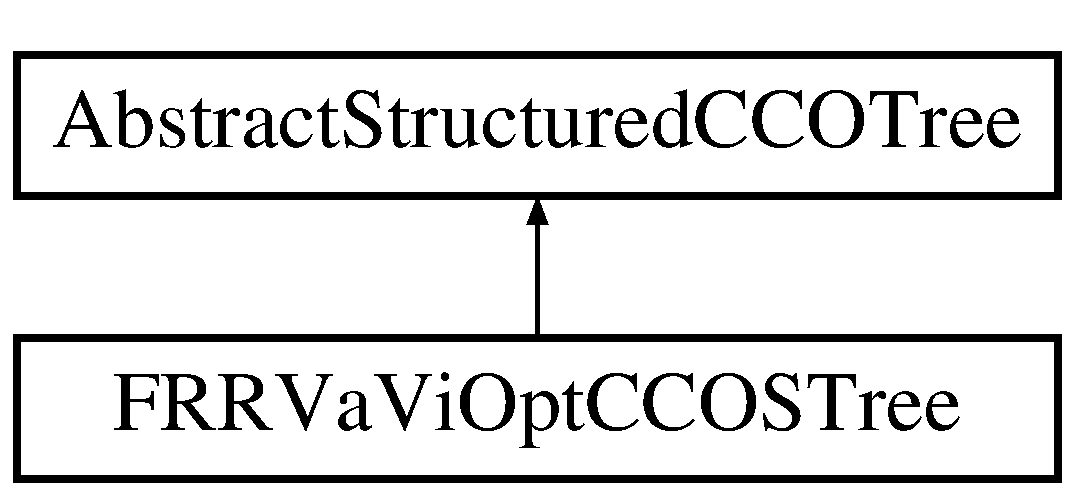
\includegraphics[height=2.000000cm]{d9/dde/class_f_r_r_va_vi_opt_c_c_o_s_tree}
\end{center}
\end{figure}
\subsection*{Public Member Functions}
\begin{DoxyCompactItemize}
\item 
\hyperlink{class_f_r_r_va_vi_opt_c_c_o_s_tree_ae9de8306c3492b1b59df21e1aa39a2ec}{F\+R\+R\+Va\+Vi\+Opt\+C\+C\+O\+S\+Tree} (\hyperlink{structpoint}{point} xi, double \hyperlink{class_f_r_r_va_vi_opt_c_c_o_s_tree_a459526bb36610ba6131cdfd788f9025b}{root\+Radius}, double qi, \hyperlink{class_abstract_constraint_function}{Abstract\+Constraint\+Function}$<$ double, int $>$ $\ast$gam, \hyperlink{class_abstract_constraint_function}{Abstract\+Constraint\+Function}$<$ double, int $>$ $\ast$eps\+Lim, \hyperlink{class_abstract_constraint_function}{Abstract\+Constraint\+Function}$<$ double, int $>$ $\ast$nu, double min\+Angle, double ref\+Pressure, double resistance\+Variation\+Tolerance, \hyperlink{class_generator_data}{Generator\+Data} $\ast$\hyperlink{class_abstract_structured_c_c_o_tree_af1836d7ed2156f3cf9cc311edfdc49b1}{instance\+Data})
\item 
\hyperlink{class_f_r_r_va_vi_opt_c_c_o_s_tree_acb93586a162c23493347db65deae06df}{F\+R\+R\+Va\+Vi\+Opt\+C\+C\+O\+S\+Tree} (string filename\+C\+CO, string filename\+V\+TK, \hyperlink{class_generator_data}{Generator\+Data} $\ast$\hyperlink{class_abstract_structured_c_c_o_tree_af1836d7ed2156f3cf9cc311edfdc49b1}{instance\+Data})
\item 
\hyperlink{class_f_r_r_va_vi_opt_c_c_o_s_tree_a50692a5fade1f64055872e81705198e5}{$\sim$\+F\+R\+R\+Va\+Vi\+Opt\+C\+C\+O\+S\+Tree} ()
\item 
\hyperlink{class_f_r_r_va_vi_opt_c_c_o_s_tree}{F\+R\+R\+Va\+Vi\+Opt\+C\+C\+O\+S\+Tree} $\ast$ \hyperlink{class_f_r_r_va_vi_opt_c_c_o_s_tree_acddc90c3f029e2c3f359e4529aa0fc3b}{clone} ()
\item 
void \hyperlink{class_f_r_r_va_vi_opt_c_c_o_s_tree_a8360ecbbf60ee0e52d4a83f40a3f0154}{get\+Closest\+Tree\+Point} (\hyperlink{structpoint}{point} x\+New, \hyperlink{structpoint}{point} $\ast$x\+Bif, double $\ast$dist)
\item 
vector$<$ \hyperlink{structvessel}{vessel} $\ast$ $>$ \hyperlink{class_f_r_r_va_vi_opt_c_c_o_s_tree_a88826c9f37705bcce03374d920eff19a}{get\+Close\+Segments} (\hyperlink{structpoint}{point} x\+New, \hyperlink{class_abstract_domain}{Abstract\+Domain} $\ast$domain, int $\ast$n\+Found)
\item 
void \hyperlink{class_f_r_r_va_vi_opt_c_c_o_s_tree_a95c4523a6c2ed20c16d83b62ec6b5873}{add\+Vessel} (\hyperlink{structpoint}{point} x\+Prox, \hyperlink{structpoint}{point} x\+Dist, \hyperlink{structvessel}{vessel} $\ast$parent)
\item 
int \hyperlink{class_f_r_r_va_vi_opt_c_c_o_s_tree_adb9397798ff7ca8cecbab33245e7fe2a}{test\+Vessel} (\hyperlink{structpoint}{point} x\+New, \hyperlink{structvessel}{vessel} $\ast$parent, \hyperlink{class_abstract_domain}{Abstract\+Domain} $\ast$domain, vector$<$ \hyperlink{structvessel}{vessel} $\ast$ $>$ neighbors, double dlim, \hyperlink{structpoint}{point} $\ast$x\+Bif, double $\ast$cost)
\item 
void \hyperlink{class_f_r_r_va_vi_opt_c_c_o_s_tree_a3e332df98c4a3fc66455aea22d563cf8}{print} ()
\item 
string \hyperlink{class_f_r_r_va_vi_opt_c_c_o_s_tree_a3c7f7ca4242f71697c421298b3ab968b}{get\+Tree\+Name} ()
\item 
double \hyperlink{class_f_r_r_va_vi_opt_c_c_o_s_tree_ae86b6d6890262180b555166853190dd1}{get\+Root\+Radius} ()
\end{DoxyCompactItemize}
\subsection*{Protected Member Functions}
\begin{DoxyCompactItemize}
\item 
void \hyperlink{class_f_r_r_va_vi_opt_c_c_o_s_tree_af4d961db2a4b60ea9bafde5cbf6758c6}{save\+Tree} (ofstream $\ast$out\+File)
\end{DoxyCompactItemize}
\subsection*{Private Member Functions}
\begin{DoxyCompactItemize}
\item 
\hyperlink{class_f_r_r_va_vi_opt_c_c_o_s_tree}{F\+R\+R\+Va\+Vi\+Opt\+C\+C\+O\+S\+Tree} $\ast$ \hyperlink{class_f_r_r_va_vi_opt_c_c_o_s_tree_af632401d7f152f10e1bcbb0d712a7b74}{clone\+Up\+To} (int levels, \hyperlink{structvessel}{vessel} $\ast$parent)
\item 
\hyperlink{structvessel}{vessel} $\ast$ \hyperlink{class_f_r_r_va_vi_opt_c_c_o_s_tree_ac0e29742975e8046b571d6d18dbd6aa3}{clone\+Tree} (\hyperlink{structvessel}{vessel} $\ast$root, vector$<$ \hyperlink{structvessel}{vessel} $\ast$ $>$ $\ast$segments)
\item 
double \hyperlink{class_f_r_r_va_vi_opt_c_c_o_s_tree_ad2e4435cea4b58085a9c7fc391490e8c}{evaluate} (\hyperlink{structpoint}{point} x\+New, \hyperlink{structpoint}{point} x\+Test, \hyperlink{structvessel}{vessel} $\ast$parent)
\item 
void \hyperlink{class_f_r_r_va_vi_opt_c_c_o_s_tree_a5f6953a55f1539ac4899e9a2e4f2ad7f}{update\+Tree} (\hyperlink{structvessel}{vessel} $\ast$root, \hyperlink{class_f_r_r_va_vi_opt_c_c_o_s_tree}{F\+R\+R\+Va\+Vi\+Opt\+C\+C\+O\+S\+Tree} $\ast$tree)
\item 
int \hyperlink{class_f_r_r_va_vi_opt_c_c_o_s_tree_a1988a62d4a8f82c547e241dc80a14fba}{is\+Symmetrically\+Valid} (double beta1, double beta2, int n\+Level)
\item 
int \hyperlink{class_f_r_r_va_vi_opt_c_c_o_s_tree_a55d5c516893c2ac1875be023548e568b}{are\+Valid\+Angles} (\hyperlink{structpoint}{point} x\+Bif, \hyperlink{structpoint}{point} x\+New, \hyperlink{structvessel}{vessel} $\ast$parent)
\item 
int \hyperlink{class_f_r_r_va_vi_opt_c_c_o_s_tree_a92eb08cc90eab3a24397efce436ebaec}{is\+Overlapped} (\hyperlink{structpoint}{point} x\+Bif, \hyperlink{structpoint}{point} x\+New, \hyperlink{structvessel}{vessel} $\ast$parent, double d\+Lim)
\item 
int \hyperlink{class_f_r_r_va_vi_opt_c_c_o_s_tree_acfbd6fe1356a89831bfc1cc137473455}{is\+Intersecting\+Vessels} (\hyperlink{structpoint}{point} p1, \hyperlink{structpoint}{point} p2, \hyperlink{structvessel}{vessel} $\ast$parent, vector$<$ \hyperlink{structvessel}{vessel} $\ast$ $>$ neighbors)
\item 
void \hyperlink{class_f_r_r_va_vi_opt_c_c_o_s_tree_ac07772412c7554ae527a756ec652a44f}{update\+Tree\+Viscosities\+Resistance} (\hyperlink{structvessel}{vessel} $\ast$root, double parent\+Radius, double $\ast$max\+Resistance\+Variation)
\item 
void \hyperlink{class_f_r_r_va_vi_opt_c_c_o_s_tree_acd9ceb8141bb7df82101a33ae5180b63}{update\+Tree\+Viscosities\+Beta} (\hyperlink{structvessel}{vessel} $\ast$root, double parent\+Radius, double $\ast$max\+Beta\+Variation)
\item 
double \hyperlink{class_f_r_r_va_vi_opt_c_c_o_s_tree_a05093832a77a583f373747ac4787808d}{get\+Nu\+FL} (double radius)
\end{DoxyCompactItemize}
\subsection*{Private Attributes}
\begin{DoxyCompactItemize}
\item 
double \hyperlink{class_f_r_r_va_vi_opt_c_c_o_s_tree_a459526bb36610ba6131cdfd788f9025b}{root\+Radius}
\item 
double \hyperlink{class_f_r_r_va_vi_opt_c_c_o_s_tree_a3652da4e84bd04dcde60101b06f2cc08}{variation\+Tolerance}
\end{DoxyCompactItemize}
\subsection*{Additional Inherited Members}


\subsection{Detailed Description}
Models a single C\+CO tree which contains the vessel\textquotesingle{}s data and connectivity. It is a variation of the algorithm 5 of Queiroz Ph.\+D. Thesis endowed with H\+PC capabilities such as parallel vessel testing and partial tree functional estimation. Current implementation is in Open\+MP although vessel testing should be executing in M\+PI and bifurcation testing in Open\+MP for best results. Specifications\+:
\begin{DoxyItemize}
\item Fixed domain;
\item Given flow Q;
\item Given pressure gradient;
\item Given N terminals;
\item Constant/variable symmetry per tree level;
\item Constant/variable Murray coefficient per tree level;
\item Variable viscosity according to Fahraeus-\/\+Lindquist model. 
\end{DoxyItemize}

\subsection{Constructor \& Destructor Documentation}
\index{F\+R\+R\+Va\+Vi\+Opt\+C\+C\+O\+S\+Tree@{F\+R\+R\+Va\+Vi\+Opt\+C\+C\+O\+S\+Tree}!F\+R\+R\+Va\+Vi\+Opt\+C\+C\+O\+S\+Tree@{F\+R\+R\+Va\+Vi\+Opt\+C\+C\+O\+S\+Tree}}
\index{F\+R\+R\+Va\+Vi\+Opt\+C\+C\+O\+S\+Tree@{F\+R\+R\+Va\+Vi\+Opt\+C\+C\+O\+S\+Tree}!F\+R\+R\+Va\+Vi\+Opt\+C\+C\+O\+S\+Tree@{F\+R\+R\+Va\+Vi\+Opt\+C\+C\+O\+S\+Tree}}
\subsubsection[{\texorpdfstring{F\+R\+R\+Va\+Vi\+Opt\+C\+C\+O\+S\+Tree(point xi, double root\+Radius, double qi, Abstract\+Constraint\+Function$<$ double, int $>$ $\ast$gam, Abstract\+Constraint\+Function$<$ double, int $>$ $\ast$eps\+Lim, Abstract\+Constraint\+Function$<$ double, int $>$ $\ast$nu, double min\+Angle, double ref\+Pressure, double resistance\+Variation\+Tolerance, Generator\+Data $\ast$instance\+Data)}{FRRVaViOptCCOSTree(point xi, double rootRadius, double qi, AbstractConstraintFunction< double, int > *gam, AbstractConstraintFunction< double, int > *epsLim, AbstractConstraintFunction< double, int > *nu, double minAngle, double refPressure, double resistanceVariationTolerance, GeneratorData *instanceData)}}]{\setlength{\rightskip}{0pt plus 5cm}F\+R\+R\+Va\+Vi\+Opt\+C\+C\+O\+S\+Tree\+::\+F\+R\+R\+Va\+Vi\+Opt\+C\+C\+O\+S\+Tree (
\begin{DoxyParamCaption}
\item[{{\bf point}}]{xi, }
\item[{double}]{root\+Radius, }
\item[{double}]{qi, }
\item[{{\bf Abstract\+Constraint\+Function}$<$ double, int $>$ $\ast$}]{gam, }
\item[{{\bf Abstract\+Constraint\+Function}$<$ double, int $>$ $\ast$}]{eps\+Lim, }
\item[{{\bf Abstract\+Constraint\+Function}$<$ double, int $>$ $\ast$}]{nu, }
\item[{double}]{min\+Angle, }
\item[{double}]{ref\+Pressure, }
\item[{double}]{resistance\+Variation\+Tolerance, }
\item[{{\bf Generator\+Data} $\ast$}]{instance\+Data}
\end{DoxyParamCaption}
)}\hypertarget{class_f_r_r_va_vi_opt_c_c_o_s_tree_ae9de8306c3492b1b59df21e1aa39a2ec}{}\label{class_f_r_r_va_vi_opt_c_c_o_s_tree_ae9de8306c3492b1b59df21e1aa39a2ec}
Common tree creator. 
\begin{DoxyParams}{Parameters}
{\em xi} & Root point. \\
\hline
{\em root\+Radius} & Root radius. \\
\hline
{\em qi} & Flow at the root. \\
\hline
{\em gam} & Murray law function. \\
\hline
{\em eps\+Lim} & Sibling vessels ratio function. \\
\hline
{\em nu} & Viscosity function with respect to the tree level. \\
\hline
{\em min\+Angle} & Minimum angle allowed. \\
\hline
{\em resistance\+Variation\+Tolerance} & Convergence tolerance for the iterative viscosity scheme. \\
\hline
\end{DoxyParams}
\index{F\+R\+R\+Va\+Vi\+Opt\+C\+C\+O\+S\+Tree@{F\+R\+R\+Va\+Vi\+Opt\+C\+C\+O\+S\+Tree}!F\+R\+R\+Va\+Vi\+Opt\+C\+C\+O\+S\+Tree@{F\+R\+R\+Va\+Vi\+Opt\+C\+C\+O\+S\+Tree}}
\index{F\+R\+R\+Va\+Vi\+Opt\+C\+C\+O\+S\+Tree@{F\+R\+R\+Va\+Vi\+Opt\+C\+C\+O\+S\+Tree}!F\+R\+R\+Va\+Vi\+Opt\+C\+C\+O\+S\+Tree@{F\+R\+R\+Va\+Vi\+Opt\+C\+C\+O\+S\+Tree}}
\subsubsection[{\texorpdfstring{F\+R\+R\+Va\+Vi\+Opt\+C\+C\+O\+S\+Tree(string filename\+C\+C\+O, string filename\+V\+T\+K, Generator\+Data $\ast$instance\+Data)}{FRRVaViOptCCOSTree(string filenameCCO, string filenameVTK, GeneratorData *instanceData)}}]{\setlength{\rightskip}{0pt plus 5cm}F\+R\+R\+Va\+Vi\+Opt\+C\+C\+O\+S\+Tree\+::\+F\+R\+R\+Va\+Vi\+Opt\+C\+C\+O\+S\+Tree (
\begin{DoxyParamCaption}
\item[{string}]{filename\+C\+CO, }
\item[{string}]{filename\+V\+TK, }
\item[{{\bf Generator\+Data} $\ast$}]{instance\+Data}
\end{DoxyParamCaption}
)}\hypertarget{class_f_r_r_va_vi_opt_c_c_o_s_tree_acb93586a162c23493347db65deae06df}{}\label{class_f_r_r_va_vi_opt_c_c_o_s_tree_acb93586a162c23493347db65deae06df}
Creates a new tree from the .cco file {\ttfamily filename}. The obtained tree has not vtk\+Line objects of the vessels. 
\begin{DoxyParams}{Parameters}
{\em filename\+C\+CO} & Path to the .cco file. \\
\hline
{\em filename\+V\+TK} & Path to the .vtk file. \\
\hline
\end{DoxyParams}
\index{F\+R\+R\+Va\+Vi\+Opt\+C\+C\+O\+S\+Tree@{F\+R\+R\+Va\+Vi\+Opt\+C\+C\+O\+S\+Tree}!````~F\+R\+R\+Va\+Vi\+Opt\+C\+C\+O\+S\+Tree@{$\sim$\+F\+R\+R\+Va\+Vi\+Opt\+C\+C\+O\+S\+Tree}}
\index{````~F\+R\+R\+Va\+Vi\+Opt\+C\+C\+O\+S\+Tree@{$\sim$\+F\+R\+R\+Va\+Vi\+Opt\+C\+C\+O\+S\+Tree}!F\+R\+R\+Va\+Vi\+Opt\+C\+C\+O\+S\+Tree@{F\+R\+R\+Va\+Vi\+Opt\+C\+C\+O\+S\+Tree}}
\subsubsection[{\texorpdfstring{$\sim$\+F\+R\+R\+Va\+Vi\+Opt\+C\+C\+O\+S\+Tree()}{~FRRVaViOptCCOSTree()}}]{\setlength{\rightskip}{0pt plus 5cm}F\+R\+R\+Va\+Vi\+Opt\+C\+C\+O\+S\+Tree\+::$\sim$\+F\+R\+R\+Va\+Vi\+Opt\+C\+C\+O\+S\+Tree (
\begin{DoxyParamCaption}
{}
\end{DoxyParamCaption}
)}\hypertarget{class_f_r_r_va_vi_opt_c_c_o_s_tree_a50692a5fade1f64055872e81705198e5}{}\label{class_f_r_r_va_vi_opt_c_c_o_s_tree_a50692a5fade1f64055872e81705198e5}
Common destructor. 

\subsection{Member Function Documentation}
\index{F\+R\+R\+Va\+Vi\+Opt\+C\+C\+O\+S\+Tree@{F\+R\+R\+Va\+Vi\+Opt\+C\+C\+O\+S\+Tree}!add\+Vessel@{add\+Vessel}}
\index{add\+Vessel@{add\+Vessel}!F\+R\+R\+Va\+Vi\+Opt\+C\+C\+O\+S\+Tree@{F\+R\+R\+Va\+Vi\+Opt\+C\+C\+O\+S\+Tree}}
\subsubsection[{\texorpdfstring{add\+Vessel(point x\+Prox, point x\+Dist, vessel $\ast$parent)}{addVessel(point xProx, point xDist, vessel *parent)}}]{\setlength{\rightskip}{0pt plus 5cm}void F\+R\+R\+Va\+Vi\+Opt\+C\+C\+O\+S\+Tree\+::add\+Vessel (
\begin{DoxyParamCaption}
\item[{{\bf point}}]{x\+Prox, }
\item[{{\bf point}}]{x\+Dist, }
\item[{{\bf vessel} $\ast$}]{parent}
\end{DoxyParamCaption}
)\hspace{0.3cm}{\ttfamily [virtual]}}\hypertarget{class_f_r_r_va_vi_opt_c_c_o_s_tree_a95c4523a6c2ed20c16d83b62ec6b5873}{}\label{class_f_r_r_va_vi_opt_c_c_o_s_tree_a95c4523a6c2ed20c16d83b62ec6b5873}
Adds a new vessel to the C\+CO tree. 
\begin{DoxyParams}{Parameters}
{\em x\+Prox} & and \\
\hline
{\em x\+Dist} & are the proximal and distal nodes of the new vessel and \\
\hline
{\em parent} & is the attachment parent vessel. \\
\hline
{\em x\+Prox} & Proximal point of the new vessel. \\
\hline
{\em x\+Dist} & Distal point of the new vessel. \\
\hline
{\em parent} & Parent to the new vessel. \\
\hline
\end{DoxyParams}


Implements \hyperlink{class_abstract_structured_c_c_o_tree_af592741d1d89d62834e9d58a72cb40af}{Abstract\+Structured\+C\+C\+O\+Tree}.

\index{F\+R\+R\+Va\+Vi\+Opt\+C\+C\+O\+S\+Tree@{F\+R\+R\+Va\+Vi\+Opt\+C\+C\+O\+S\+Tree}!are\+Valid\+Angles@{are\+Valid\+Angles}}
\index{are\+Valid\+Angles@{are\+Valid\+Angles}!F\+R\+R\+Va\+Vi\+Opt\+C\+C\+O\+S\+Tree@{F\+R\+R\+Va\+Vi\+Opt\+C\+C\+O\+S\+Tree}}
\subsubsection[{\texorpdfstring{are\+Valid\+Angles(point x\+Bif, point x\+New, vessel $\ast$parent)}{areValidAngles(point xBif, point xNew, vessel *parent)}}]{\setlength{\rightskip}{0pt plus 5cm}int F\+R\+R\+Va\+Vi\+Opt\+C\+C\+O\+S\+Tree\+::are\+Valid\+Angles (
\begin{DoxyParamCaption}
\item[{{\bf point}}]{x\+Bif, }
\item[{{\bf point}}]{x\+New, }
\item[{{\bf vessel} $\ast$}]{parent}
\end{DoxyParamCaption}
)\hspace{0.3cm}{\ttfamily [private]}}\hypertarget{class_f_r_r_va_vi_opt_c_c_o_s_tree_a55d5c516893c2ac1875be023548e568b}{}\label{class_f_r_r_va_vi_opt_c_c_o_s_tree_a55d5c516893c2ac1875be023548e568b}
Checks if the angles of the parent vessel and the new vessel do not violate the minimum angle constraint. 
\begin{DoxyParams}{Parameters}
{\em x\+Bif} & Bifurcation point between the new vessel and the distal part of the parent vessel (i\+Con). \\
\hline
{\em x\+New} & Distal point of the new vessel. \\
\hline
{\em parent} & Parent vessel. \\
\hline
\end{DoxyParams}
\begin{DoxyReturn}{Returns}
If the angles are higher than the minimum allowed. 
\end{DoxyReturn}
\index{F\+R\+R\+Va\+Vi\+Opt\+C\+C\+O\+S\+Tree@{F\+R\+R\+Va\+Vi\+Opt\+C\+C\+O\+S\+Tree}!clone@{clone}}
\index{clone@{clone}!F\+R\+R\+Va\+Vi\+Opt\+C\+C\+O\+S\+Tree@{F\+R\+R\+Va\+Vi\+Opt\+C\+C\+O\+S\+Tree}}
\subsubsection[{\texorpdfstring{clone()}{clone()}}]{\setlength{\rightskip}{0pt plus 5cm}{\bf F\+R\+R\+Va\+Vi\+Opt\+C\+C\+O\+S\+Tree} $\ast$ F\+R\+R\+Va\+Vi\+Opt\+C\+C\+O\+S\+Tree\+::clone (
\begin{DoxyParamCaption}
{}
\end{DoxyParamCaption}
)}\hypertarget{class_f_r_r_va_vi_opt_c_c_o_s_tree_acddc90c3f029e2c3f359e4529aa0fc3b}{}\label{class_f_r_r_va_vi_opt_c_c_o_s_tree_acddc90c3f029e2c3f359e4529aa0fc3b}
Creates a copy from the tree without the vtk structures (neither from the tree nor from the vessels). \begin{DoxyReturn}{Returns}
Copy from the tree 
\end{DoxyReturn}
\index{F\+R\+R\+Va\+Vi\+Opt\+C\+C\+O\+S\+Tree@{F\+R\+R\+Va\+Vi\+Opt\+C\+C\+O\+S\+Tree}!clone\+Tree@{clone\+Tree}}
\index{clone\+Tree@{clone\+Tree}!F\+R\+R\+Va\+Vi\+Opt\+C\+C\+O\+S\+Tree@{F\+R\+R\+Va\+Vi\+Opt\+C\+C\+O\+S\+Tree}}
\subsubsection[{\texorpdfstring{clone\+Tree(vessel $\ast$root, vector$<$ vessel $\ast$ $>$ $\ast$segments)}{cloneTree(vessel *root, vector< vessel * > *segments)}}]{\setlength{\rightskip}{0pt plus 5cm}{\bf vessel} $\ast$ F\+R\+R\+Va\+Vi\+Opt\+C\+C\+O\+S\+Tree\+::clone\+Tree (
\begin{DoxyParamCaption}
\item[{{\bf vessel} $\ast$}]{root, }
\item[{vector$<$ {\bf vessel} $\ast$ $>$ $\ast$}]{segments}
\end{DoxyParamCaption}
)\hspace{0.3cm}{\ttfamily [private]}}\hypertarget{class_f_r_r_va_vi_opt_c_c_o_s_tree_ac0e29742975e8046b571d6d18dbd6aa3}{}\label{class_f_r_r_va_vi_opt_c_c_o_s_tree_ac0e29742975e8046b571d6d18dbd6aa3}
Clones the subtree with parent vessel {\ttfamily root} recursively. 
\begin{DoxyParams}{Parameters}
{\em root} & Root of the tree to clone. \\
\hline
{\em segments} & Segments of the tree. \\
\hline
\end{DoxyParams}
\begin{DoxyReturn}{Returns}
Cloned subtree. 
\end{DoxyReturn}
\index{F\+R\+R\+Va\+Vi\+Opt\+C\+C\+O\+S\+Tree@{F\+R\+R\+Va\+Vi\+Opt\+C\+C\+O\+S\+Tree}!clone\+Up\+To@{clone\+Up\+To}}
\index{clone\+Up\+To@{clone\+Up\+To}!F\+R\+R\+Va\+Vi\+Opt\+C\+C\+O\+S\+Tree@{F\+R\+R\+Va\+Vi\+Opt\+C\+C\+O\+S\+Tree}}
\subsubsection[{\texorpdfstring{clone\+Up\+To(int levels, vessel $\ast$parent)}{cloneUpTo(int levels, vessel *parent)}}]{\setlength{\rightskip}{0pt plus 5cm}{\bf F\+R\+R\+Va\+Vi\+Opt\+C\+C\+O\+S\+Tree} $\ast$ F\+R\+R\+Va\+Vi\+Opt\+C\+C\+O\+S\+Tree\+::clone\+Up\+To (
\begin{DoxyParamCaption}
\item[{int}]{levels, }
\item[{{\bf vessel} $\ast$}]{parent}
\end{DoxyParamCaption}
)\hspace{0.3cm}{\ttfamily [private]}}\hypertarget{class_f_r_r_va_vi_opt_c_c_o_s_tree_af632401d7f152f10e1bcbb0d712a7b74}{}\label{class_f_r_r_va_vi_opt_c_c_o_s_tree_af632401d7f152f10e1bcbb0d712a7b74}
Clones the subtree with parent vessel {\ttfamily levels} . 
\begin{DoxyParams}{Parameters}
{\em root} & Root of the tree to clone. \\
\hline
{\em segments} & Segments of the tree. \\
\hline
\end{DoxyParams}
\begin{DoxyReturn}{Returns}
Cloned subtree. 
\end{DoxyReturn}
\index{F\+R\+R\+Va\+Vi\+Opt\+C\+C\+O\+S\+Tree@{F\+R\+R\+Va\+Vi\+Opt\+C\+C\+O\+S\+Tree}!evaluate@{evaluate}}
\index{evaluate@{evaluate}!F\+R\+R\+Va\+Vi\+Opt\+C\+C\+O\+S\+Tree@{F\+R\+R\+Va\+Vi\+Opt\+C\+C\+O\+S\+Tree}}
\subsubsection[{\texorpdfstring{evaluate(point x\+New, point x\+Test, vessel $\ast$parent)}{evaluate(point xNew, point xTest, vessel *parent)}}]{\setlength{\rightskip}{0pt plus 5cm}double F\+R\+R\+Va\+Vi\+Opt\+C\+C\+O\+S\+Tree\+::evaluate (
\begin{DoxyParamCaption}
\item[{{\bf point}}]{x\+New, }
\item[{{\bf point}}]{x\+Test, }
\item[{{\bf vessel} $\ast$}]{parent}
\end{DoxyParamCaption}
)\hspace{0.3cm}{\ttfamily [private]}}\hypertarget{class_f_r_r_va_vi_opt_c_c_o_s_tree_ad2e4435cea4b58085a9c7fc391490e8c}{}\label{class_f_r_r_va_vi_opt_c_c_o_s_tree_ad2e4435cea4b58085a9c7fc391490e8c}
Returns a partial variation of the cost functional due to the new segment inclusion. 
\begin{DoxyParams}{Parameters}
{\em x\+New} & Proximal point of the new vessel. \\
\hline
{\em x\+Test} & Distal point of the new vessel. \\
\hline
{\em parent} & Parent to the new vessel. \\
\hline
\end{DoxyParams}
\index{F\+R\+R\+Va\+Vi\+Opt\+C\+C\+O\+S\+Tree@{F\+R\+R\+Va\+Vi\+Opt\+C\+C\+O\+S\+Tree}!get\+Close\+Segments@{get\+Close\+Segments}}
\index{get\+Close\+Segments@{get\+Close\+Segments}!F\+R\+R\+Va\+Vi\+Opt\+C\+C\+O\+S\+Tree@{F\+R\+R\+Va\+Vi\+Opt\+C\+C\+O\+S\+Tree}}
\subsubsection[{\texorpdfstring{get\+Close\+Segments(point x\+New, Abstract\+Domain $\ast$domain, int $\ast$n\+Found)}{getCloseSegments(point xNew, AbstractDomain *domain, int *nFound)}}]{\setlength{\rightskip}{0pt plus 5cm}vector$<$ {\bf vessel} $\ast$ $>$ F\+R\+R\+Va\+Vi\+Opt\+C\+C\+O\+S\+Tree\+::get\+Close\+Segments (
\begin{DoxyParamCaption}
\item[{{\bf point}}]{x\+New, }
\item[{{\bf Abstract\+Domain} $\ast$}]{domain, }
\item[{int $\ast$}]{n\+Found}
\end{DoxyParamCaption}
)\hspace{0.3cm}{\ttfamily [virtual]}}\hypertarget{class_f_r_r_va_vi_opt_c_c_o_s_tree_a88826c9f37705bcce03374d920eff19a}{}\label{class_f_r_r_va_vi_opt_c_c_o_s_tree_a88826c9f37705bcce03374d920eff19a}
Return the segments in a close neighborhood of {\ttfamily x\+New}. The neighborhood is computed based on the perfusion volume indicated by {\ttfamily domain}. 
\begin{DoxyParams}{Parameters}
{\em x\+New} & Center point of the neighborhood of interest. \\
\hline
{\em domain} & Domain of the segments. \\
\hline
{\em n\+Found} & Amount of segments in the neighborhood. \\
\hline
\end{DoxyParams}
\begin{DoxyReturn}{Returns}
Array of segments in the neighborhood of {\ttfamily x\+New}. 
\end{DoxyReturn}


Implements \hyperlink{class_abstract_structured_c_c_o_tree_a0371a4c9a5e8ddfd8b0cc8d811d60f04}{Abstract\+Structured\+C\+C\+O\+Tree}.

\index{F\+R\+R\+Va\+Vi\+Opt\+C\+C\+O\+S\+Tree@{F\+R\+R\+Va\+Vi\+Opt\+C\+C\+O\+S\+Tree}!get\+Closest\+Tree\+Point@{get\+Closest\+Tree\+Point}}
\index{get\+Closest\+Tree\+Point@{get\+Closest\+Tree\+Point}!F\+R\+R\+Va\+Vi\+Opt\+C\+C\+O\+S\+Tree@{F\+R\+R\+Va\+Vi\+Opt\+C\+C\+O\+S\+Tree}}
\subsubsection[{\texorpdfstring{get\+Closest\+Tree\+Point(point x\+New, point $\ast$x\+Bif, double $\ast$dist)}{getClosestTreePoint(point xNew, point *xBif, double *dist)}}]{\setlength{\rightskip}{0pt plus 5cm}void F\+R\+R\+Va\+Vi\+Opt\+C\+C\+O\+S\+Tree\+::get\+Closest\+Tree\+Point (
\begin{DoxyParamCaption}
\item[{{\bf point}}]{x\+New, }
\item[{{\bf point} $\ast$}]{x\+Bif, }
\item[{double $\ast$}]{dist}
\end{DoxyParamCaption}
)\hspace{0.3cm}{\ttfamily [virtual]}}\hypertarget{class_f_r_r_va_vi_opt_c_c_o_s_tree_a8360ecbbf60ee0e52d4a83f40a3f0154}{}\label{class_f_r_r_va_vi_opt_c_c_o_s_tree_a8360ecbbf60ee0e52d4a83f40a3f0154}
Returns the closest point in the C\+C\+O\+Tree with respect to {\ttfamily x\+New} point. 
\begin{DoxyParams}{Parameters}
{\em x\+New} & Point from which the minimum distance is computed. \\
\hline
{\em x\+Bif} & Closest point in the tree to {\ttfamily x\+New}. \\
\hline
{\em dist} & Minimum distance between {\ttfamily x\+New} and the tree. \\
\hline
\end{DoxyParams}


Implements \hyperlink{class_abstract_structured_c_c_o_tree_a09cb70d5e23065273d87dd0c0434e1c5}{Abstract\+Structured\+C\+C\+O\+Tree}.

\index{F\+R\+R\+Va\+Vi\+Opt\+C\+C\+O\+S\+Tree@{F\+R\+R\+Va\+Vi\+Opt\+C\+C\+O\+S\+Tree}!get\+Nu\+FL@{get\+Nu\+FL}}
\index{get\+Nu\+FL@{get\+Nu\+FL}!F\+R\+R\+Va\+Vi\+Opt\+C\+C\+O\+S\+Tree@{F\+R\+R\+Va\+Vi\+Opt\+C\+C\+O\+S\+Tree}}
\subsubsection[{\texorpdfstring{get\+Nu\+F\+L(double radius)}{getNuFL(double radius)}}]{\setlength{\rightskip}{0pt plus 5cm}double F\+R\+R\+Va\+Vi\+Opt\+C\+C\+O\+S\+Tree\+::get\+Nu\+FL (
\begin{DoxyParamCaption}
\item[{double}]{radius}
\end{DoxyParamCaption}
)\hspace{0.3cm}{\ttfamily [inline]}, {\ttfamily [private]}}\hypertarget{class_f_r_r_va_vi_opt_c_c_o_s_tree_a05093832a77a583f373747ac4787808d}{}\label{class_f_r_r_va_vi_opt_c_c_o_s_tree_a05093832a77a583f373747ac4787808d}
Returns the viscosity estimated with the Fahraeus-\/\+Lindquist model. 
\begin{DoxyParams}{Parameters}
{\em radius} & \\
\hline
\end{DoxyParams}
\begin{DoxyReturn}{Returns}
Viscosity value. 
\end{DoxyReturn}
\index{F\+R\+R\+Va\+Vi\+Opt\+C\+C\+O\+S\+Tree@{F\+R\+R\+Va\+Vi\+Opt\+C\+C\+O\+S\+Tree}!get\+Root\+Radius@{get\+Root\+Radius}}
\index{get\+Root\+Radius@{get\+Root\+Radius}!F\+R\+R\+Va\+Vi\+Opt\+C\+C\+O\+S\+Tree@{F\+R\+R\+Va\+Vi\+Opt\+C\+C\+O\+S\+Tree}}
\subsubsection[{\texorpdfstring{get\+Root\+Radius()}{getRootRadius()}}]{\setlength{\rightskip}{0pt plus 5cm}double F\+R\+R\+Va\+Vi\+Opt\+C\+C\+O\+S\+Tree\+::get\+Root\+Radius (
\begin{DoxyParamCaption}
{}
\end{DoxyParamCaption}
)}\hypertarget{class_f_r_r_va_vi_opt_c_c_o_s_tree_ae86b6d6890262180b555166853190dd1}{}\label{class_f_r_r_va_vi_opt_c_c_o_s_tree_ae86b6d6890262180b555166853190dd1}
Returns the root radius. \begin{DoxyReturn}{Returns}
Root radius. 
\end{DoxyReturn}
\index{F\+R\+R\+Va\+Vi\+Opt\+C\+C\+O\+S\+Tree@{F\+R\+R\+Va\+Vi\+Opt\+C\+C\+O\+S\+Tree}!get\+Tree\+Name@{get\+Tree\+Name}}
\index{get\+Tree\+Name@{get\+Tree\+Name}!F\+R\+R\+Va\+Vi\+Opt\+C\+C\+O\+S\+Tree@{F\+R\+R\+Va\+Vi\+Opt\+C\+C\+O\+S\+Tree}}
\subsubsection[{\texorpdfstring{get\+Tree\+Name()}{getTreeName()}}]{\setlength{\rightskip}{0pt plus 5cm}string F\+R\+R\+Va\+Vi\+Opt\+C\+C\+O\+S\+Tree\+::get\+Tree\+Name (
\begin{DoxyParamCaption}
{}
\end{DoxyParamCaption}
)\hspace{0.3cm}{\ttfamily [virtual]}}\hypertarget{class_f_r_r_va_vi_opt_c_c_o_s_tree_a3c7f7ca4242f71697c421298b3ab968b}{}\label{class_f_r_r_va_vi_opt_c_c_o_s_tree_a3c7f7ca4242f71697c421298b3ab968b}
Returns the class name identifier. \begin{DoxyReturn}{Returns}
Class name. 
\end{DoxyReturn}


Implements \hyperlink{class_abstract_structured_c_c_o_tree_a32e56a263498bc04c3c552fc7de30554}{Abstract\+Structured\+C\+C\+O\+Tree}.

\index{F\+R\+R\+Va\+Vi\+Opt\+C\+C\+O\+S\+Tree@{F\+R\+R\+Va\+Vi\+Opt\+C\+C\+O\+S\+Tree}!is\+Intersecting\+Vessels@{is\+Intersecting\+Vessels}}
\index{is\+Intersecting\+Vessels@{is\+Intersecting\+Vessels}!F\+R\+R\+Va\+Vi\+Opt\+C\+C\+O\+S\+Tree@{F\+R\+R\+Va\+Vi\+Opt\+C\+C\+O\+S\+Tree}}
\subsubsection[{\texorpdfstring{is\+Intersecting\+Vessels(point p1, point p2, vessel $\ast$parent, vector$<$ vessel $\ast$ $>$ neighbors)}{isIntersectingVessels(point p1, point p2, vessel *parent, vector< vessel * > neighbors)}}]{\setlength{\rightskip}{0pt plus 5cm}int F\+R\+R\+Va\+Vi\+Opt\+C\+C\+O\+S\+Tree\+::is\+Intersecting\+Vessels (
\begin{DoxyParamCaption}
\item[{{\bf point}}]{p1, }
\item[{{\bf point}}]{p2, }
\item[{{\bf vessel} $\ast$}]{parent, }
\item[{vector$<$ {\bf vessel} $\ast$ $>$}]{neighbors}
\end{DoxyParamCaption}
)\hspace{0.3cm}{\ttfamily [private]}}\hypertarget{class_f_r_r_va_vi_opt_c_c_o_s_tree_acfbd6fe1356a89831bfc1cc137473455}{}\label{class_f_r_r_va_vi_opt_c_c_o_s_tree_acfbd6fe1356a89831bfc1cc137473455}
It returns if the line 
\begin{DoxyParams}{Parameters}
{\em p1} & -\/ \\
\hline
{\em p2} & intersects any vessel of the tree beside parent. \\
\hline
{\em p1} & Extreme point 1 of the line. \\
\hline
{\em p2} & Extreme point 2 of the line. \\
\hline
{\em parent} & Vessel excluded from the checking. \\
\hline
{\em boundary\+Tol} & Factor of line contraction at the extremes to avoid false intersections due to contact with anastomose. \\
\hline
\end{DoxyParams}
\begin{DoxyReturn}{Returns}
If the segment intersects any segment of the tree. 
\end{DoxyReturn}
\index{F\+R\+R\+Va\+Vi\+Opt\+C\+C\+O\+S\+Tree@{F\+R\+R\+Va\+Vi\+Opt\+C\+C\+O\+S\+Tree}!is\+Overlapped@{is\+Overlapped}}
\index{is\+Overlapped@{is\+Overlapped}!F\+R\+R\+Va\+Vi\+Opt\+C\+C\+O\+S\+Tree@{F\+R\+R\+Va\+Vi\+Opt\+C\+C\+O\+S\+Tree}}
\subsubsection[{\texorpdfstring{is\+Overlapped(point x\+Bif, point x\+New, vessel $\ast$parent, double d\+Lim)}{isOverlapped(point xBif, point xNew, vessel *parent, double dLim)}}]{\setlength{\rightskip}{0pt plus 5cm}int F\+R\+R\+Va\+Vi\+Opt\+C\+C\+O\+S\+Tree\+::is\+Overlapped (
\begin{DoxyParamCaption}
\item[{{\bf point}}]{x\+Bif, }
\item[{{\bf point}}]{x\+New, }
\item[{{\bf vessel} $\ast$}]{parent, }
\item[{double}]{d\+Lim}
\end{DoxyParamCaption}
)\hspace{0.3cm}{\ttfamily [private]}}\hypertarget{class_f_r_r_va_vi_opt_c_c_o_s_tree_a92eb08cc90eab3a24397efce436ebaec}{}\label{class_f_r_r_va_vi_opt_c_c_o_s_tree_a92eb08cc90eab3a24397efce436ebaec}
Determines if the segment x\+Bif-\/x\+New is closer than d\+Lim to any other segment of the tree (without being its parent vessel). Not used. 
\begin{DoxyParams}{Parameters}
{\em x\+Bif} & Proximal point for the new segment. \\
\hline
{\em x\+New} & Distal point for the new segment. \\
\hline
{\em parent} & Parent vessel of the new segment. \\
\hline
{\em d\+Lim} & Perfusion volume for each terminal at the current state of the tree. \\
\hline
\end{DoxyParams}
\begin{DoxyReturn}{Returns}
If the middle point of the segment is sufficiently distant from the tree. 
\end{DoxyReturn}
\index{F\+R\+R\+Va\+Vi\+Opt\+C\+C\+O\+S\+Tree@{F\+R\+R\+Va\+Vi\+Opt\+C\+C\+O\+S\+Tree}!is\+Symmetrically\+Valid@{is\+Symmetrically\+Valid}}
\index{is\+Symmetrically\+Valid@{is\+Symmetrically\+Valid}!F\+R\+R\+Va\+Vi\+Opt\+C\+C\+O\+S\+Tree@{F\+R\+R\+Va\+Vi\+Opt\+C\+C\+O\+S\+Tree}}
\subsubsection[{\texorpdfstring{is\+Symmetrically\+Valid(double beta1, double beta2, int n\+Level)}{isSymmetricallyValid(double beta1, double beta2, int nLevel)}}]{\setlength{\rightskip}{0pt plus 5cm}int F\+R\+R\+Va\+Vi\+Opt\+C\+C\+O\+S\+Tree\+::is\+Symmetrically\+Valid (
\begin{DoxyParamCaption}
\item[{double}]{beta1, }
\item[{double}]{beta2, }
\item[{int}]{n\+Level}
\end{DoxyParamCaption}
)\hspace{0.3cm}{\ttfamily [private]}}\hypertarget{class_f_r_r_va_vi_opt_c_c_o_s_tree_a1988a62d4a8f82c547e241dc80a14fba}{}\label{class_f_r_r_va_vi_opt_c_c_o_s_tree_a1988a62d4a8f82c547e241dc80a14fba}
For a giving pair of beta between sibling of a parent vessel, it analyze the symmetry constrain given by eps\+Lim function.


\begin{DoxyParams}{Parameters}
{\em beta1} & Beta for the 1st sibling. \\
\hline
{\em beta2} & Beta for the 2nd sibling. \\
\hline
{\em n\+Level} & Tree level of the bifurcation. \\
\hline
\end{DoxyParams}
\begin{DoxyReturn}{Returns}
If the simmetry constrain is satisfied. 
\end{DoxyReturn}
\index{F\+R\+R\+Va\+Vi\+Opt\+C\+C\+O\+S\+Tree@{F\+R\+R\+Va\+Vi\+Opt\+C\+C\+O\+S\+Tree}!print@{print}}
\index{print@{print}!F\+R\+R\+Va\+Vi\+Opt\+C\+C\+O\+S\+Tree@{F\+R\+R\+Va\+Vi\+Opt\+C\+C\+O\+S\+Tree}}
\subsubsection[{\texorpdfstring{print()}{print()}}]{\setlength{\rightskip}{0pt plus 5cm}void F\+R\+R\+Va\+Vi\+Opt\+C\+C\+O\+S\+Tree\+::print (
\begin{DoxyParamCaption}
{}
\end{DoxyParamCaption}
)\hspace{0.3cm}{\ttfamily [virtual]}}\hypertarget{class_f_r_r_va_vi_opt_c_c_o_s_tree_a3e332df98c4a3fc66455aea22d563cf8}{}\label{class_f_r_r_va_vi_opt_c_c_o_s_tree_a3e332df98c4a3fc66455aea22d563cf8}
Prints the current tree node by node. 

Implements \hyperlink{class_abstract_structured_c_c_o_tree_ab28e036b4d82004ab4bafa964d7f7c97}{Abstract\+Structured\+C\+C\+O\+Tree}.

\index{F\+R\+R\+Va\+Vi\+Opt\+C\+C\+O\+S\+Tree@{F\+R\+R\+Va\+Vi\+Opt\+C\+C\+O\+S\+Tree}!save\+Tree@{save\+Tree}}
\index{save\+Tree@{save\+Tree}!F\+R\+R\+Va\+Vi\+Opt\+C\+C\+O\+S\+Tree@{F\+R\+R\+Va\+Vi\+Opt\+C\+C\+O\+S\+Tree}}
\subsubsection[{\texorpdfstring{save\+Tree(ofstream $\ast$out\+File)}{saveTree(ofstream *outFile)}}]{\setlength{\rightskip}{0pt plus 5cm}void F\+R\+R\+Va\+Vi\+Opt\+C\+C\+O\+S\+Tree\+::save\+Tree (
\begin{DoxyParamCaption}
\item[{ofstream $\ast$}]{out\+File}
\end{DoxyParamCaption}
)\hspace{0.3cm}{\ttfamily [protected]}, {\ttfamily [virtual]}}\hypertarget{class_f_r_r_va_vi_opt_c_c_o_s_tree_af4d961db2a4b60ea9bafde5cbf6758c6}{}\label{class_f_r_r_va_vi_opt_c_c_o_s_tree_af4d961db2a4b60ea9bafde5cbf6758c6}
Returns a string with the tree atributes to create the .cco file. 
\begin{DoxyParams}{Parameters}
{\em out\+File} & File writer for the .cco file. \\
\hline
\end{DoxyParams}


Reimplemented from \hyperlink{class_abstract_structured_c_c_o_tree_a16fb849f7fa74189c6b74c60ce59e776}{Abstract\+Structured\+C\+C\+O\+Tree}.

\index{F\+R\+R\+Va\+Vi\+Opt\+C\+C\+O\+S\+Tree@{F\+R\+R\+Va\+Vi\+Opt\+C\+C\+O\+S\+Tree}!test\+Vessel@{test\+Vessel}}
\index{test\+Vessel@{test\+Vessel}!F\+R\+R\+Va\+Vi\+Opt\+C\+C\+O\+S\+Tree@{F\+R\+R\+Va\+Vi\+Opt\+C\+C\+O\+S\+Tree}}
\subsubsection[{\texorpdfstring{test\+Vessel(point x\+New, vessel $\ast$parent, Abstract\+Domain $\ast$domain, vector$<$ vessel $\ast$ $>$ neighbors, double dlim, point $\ast$x\+Bif, double $\ast$cost)}{testVessel(point xNew, vessel *parent, AbstractDomain *domain, vector< vessel * > neighbors, double dlim, point *xBif, double *cost)}}]{\setlength{\rightskip}{0pt plus 5cm}int F\+R\+R\+Va\+Vi\+Opt\+C\+C\+O\+S\+Tree\+::test\+Vessel (
\begin{DoxyParamCaption}
\item[{{\bf point}}]{x\+New, }
\item[{{\bf vessel} $\ast$}]{parent, }
\item[{{\bf Abstract\+Domain} $\ast$}]{domain, }
\item[{vector$<$ {\bf vessel} $\ast$ $>$}]{neighbors, }
\item[{double}]{dlim, }
\item[{{\bf point} $\ast$}]{x\+Bif, }
\item[{double $\ast$}]{cost}
\end{DoxyParamCaption}
)\hspace{0.3cm}{\ttfamily [virtual]}}\hypertarget{class_f_r_r_va_vi_opt_c_c_o_s_tree_adb9397798ff7ca8cecbab33245e7fe2a}{}\label{class_f_r_r_va_vi_opt_c_c_o_s_tree_adb9397798ff7ca8cecbab33245e7fe2a}
For a given spatial point {\ttfamily x\+New} test its connection with {\ttfamily parent} vessel. It must evaluate if the restrictions of geometry and symmetry are satisfied and also if it do not intersects with other vessel of this tree. It returns in {\ttfamily cost} the functional variation by the inclusion of such vessel. 
\begin{DoxyParams}{Parameters}
{\em x\+New} & Distal point for the new vessel to test. \\
\hline
{\em parent} & Parent vessel to test the {\ttfamily x\+New} point connection. \\
\hline
{\em domain} & Tree domain. \\
\hline
{\em neighbors} & Close neighbors used for intersection test. \\
\hline
{\em dlim} & Not used in the current implementation. \\
\hline
{\em x\+Bif} & Proximal point for the new vessel that present the lower function cost. \\
\hline
{\em cost} & Functional cost variation for the best bifurcation position. \\
\hline
\end{DoxyParams}
\begin{DoxyReturn}{Returns}
If the connection of the tree with x\+New is possible. If not {\ttfamily cost} is I\+N\+F\+I\+N\+I\+TY. 
\end{DoxyReturn}


Implements \hyperlink{class_abstract_structured_c_c_o_tree_ac566ae7f8357ce1f61f624d87a9daf86}{Abstract\+Structured\+C\+C\+O\+Tree}.

\index{F\+R\+R\+Va\+Vi\+Opt\+C\+C\+O\+S\+Tree@{F\+R\+R\+Va\+Vi\+Opt\+C\+C\+O\+S\+Tree}!update\+Tree@{update\+Tree}}
\index{update\+Tree@{update\+Tree}!F\+R\+R\+Va\+Vi\+Opt\+C\+C\+O\+S\+Tree@{F\+R\+R\+Va\+Vi\+Opt\+C\+C\+O\+S\+Tree}}
\subsubsection[{\texorpdfstring{update\+Tree(vessel $\ast$root, F\+R\+R\+Va\+Vi\+Opt\+C\+C\+O\+S\+Tree $\ast$tree)}{updateTree(vessel *root, FRRVaViOptCCOSTree *tree)}}]{\setlength{\rightskip}{0pt plus 5cm}void F\+R\+R\+Va\+Vi\+Opt\+C\+C\+O\+S\+Tree\+::update\+Tree (
\begin{DoxyParamCaption}
\item[{{\bf vessel} $\ast$}]{root, }
\item[{{\bf F\+R\+R\+Va\+Vi\+Opt\+C\+C\+O\+S\+Tree} $\ast$}]{tree}
\end{DoxyParamCaption}
)\hspace{0.3cm}{\ttfamily [private]}}\hypertarget{class_f_r_r_va_vi_opt_c_c_o_s_tree_a5f6953a55f1539ac4899e9a2e4f2ad7f}{}\label{class_f_r_r_va_vi_opt_c_c_o_s_tree_a5f6953a55f1539ac4899e9a2e4f2ad7f}
Updates the tree values for the current topology in only one tree \char`\"{}in order\char`\"{} swept (O(\+N)). As the recursion deepens, the level number is computed for each element. As the recursion is returning, it computes the flow and resistance for the current node and the radius ratio for its childs. 
\begin{DoxyParams}{Parameters}
{\em root} & Root vessel for the tree to update. \\
\hline
{\em tree} & Tree to update. \\
\hline
\end{DoxyParams}
\index{F\+R\+R\+Va\+Vi\+Opt\+C\+C\+O\+S\+Tree@{F\+R\+R\+Va\+Vi\+Opt\+C\+C\+O\+S\+Tree}!update\+Tree\+Viscosities\+Beta@{update\+Tree\+Viscosities\+Beta}}
\index{update\+Tree\+Viscosities\+Beta@{update\+Tree\+Viscosities\+Beta}!F\+R\+R\+Va\+Vi\+Opt\+C\+C\+O\+S\+Tree@{F\+R\+R\+Va\+Vi\+Opt\+C\+C\+O\+S\+Tree}}
\subsubsection[{\texorpdfstring{update\+Tree\+Viscosities\+Beta(vessel $\ast$root, double parent\+Radius, double $\ast$max\+Beta\+Variation)}{updateTreeViscositiesBeta(vessel *root, double parentRadius, double *maxBetaVariation)}}]{\setlength{\rightskip}{0pt plus 5cm}void F\+R\+R\+Va\+Vi\+Opt\+C\+C\+O\+S\+Tree\+::update\+Tree\+Viscosities\+Beta (
\begin{DoxyParamCaption}
\item[{{\bf vessel} $\ast$}]{root, }
\item[{double}]{parent\+Radius, }
\item[{double $\ast$}]{max\+Beta\+Variation}
\end{DoxyParamCaption}
)\hspace{0.3cm}{\ttfamily [private]}}\hypertarget{class_f_r_r_va_vi_opt_c_c_o_s_tree_acd9ceb8141bb7df82101a33ae5180b63}{}\label{class_f_r_r_va_vi_opt_c_c_o_s_tree_acd9ceb8141bb7df82101a33ae5180b63}
Updates the tree beta values for the current vessel diameters. 
\begin{DoxyParams}{Parameters}
{\em root} & Tree root. \\
\hline
{\em parent\+Radius} & 1.\+0 if root is actually the tree root, or parent radius of root otherwise. \\
\hline
{\em max\+Beta\+Variation} & The maximum variation of the beta value due to the update. \\
\hline
\end{DoxyParams}
\index{F\+R\+R\+Va\+Vi\+Opt\+C\+C\+O\+S\+Tree@{F\+R\+R\+Va\+Vi\+Opt\+C\+C\+O\+S\+Tree}!update\+Tree\+Viscosities\+Resistance@{update\+Tree\+Viscosities\+Resistance}}
\index{update\+Tree\+Viscosities\+Resistance@{update\+Tree\+Viscosities\+Resistance}!F\+R\+R\+Va\+Vi\+Opt\+C\+C\+O\+S\+Tree@{F\+R\+R\+Va\+Vi\+Opt\+C\+C\+O\+S\+Tree}}
\subsubsection[{\texorpdfstring{update\+Tree\+Viscosities\+Resistance(vessel $\ast$root, double parent\+Radius, double $\ast$max\+Resistance\+Variation)}{updateTreeViscositiesResistance(vessel *root, double parentRadius, double *maxResistanceVariation)}}]{\setlength{\rightskip}{0pt plus 5cm}void F\+R\+R\+Va\+Vi\+Opt\+C\+C\+O\+S\+Tree\+::update\+Tree\+Viscosities\+Resistance (
\begin{DoxyParamCaption}
\item[{{\bf vessel} $\ast$}]{root, }
\item[{double}]{parent\+Radius, }
\item[{double $\ast$}]{max\+Resistance\+Variation}
\end{DoxyParamCaption}
)\hspace{0.3cm}{\ttfamily [private]}}\hypertarget{class_f_r_r_va_vi_opt_c_c_o_s_tree_ac07772412c7554ae527a756ec652a44f}{}\label{class_f_r_r_va_vi_opt_c_c_o_s_tree_ac07772412c7554ae527a756ec652a44f}
Updates the tree resistance values for the current vessel diameters. 
\begin{DoxyParams}{Parameters}
{\em root} & Tree root. \\
\hline
{\em parent\+Radius} & 1.\+0 if root is actually the tree root, or parent radius of root otherwise. \\
\hline
{\em max\+Resistance\+Variation} & The maximum variation of the resistance due to the update. \\
\hline
\end{DoxyParams}


\subsection{Member Data Documentation}
\index{F\+R\+R\+Va\+Vi\+Opt\+C\+C\+O\+S\+Tree@{F\+R\+R\+Va\+Vi\+Opt\+C\+C\+O\+S\+Tree}!root\+Radius@{root\+Radius}}
\index{root\+Radius@{root\+Radius}!F\+R\+R\+Va\+Vi\+Opt\+C\+C\+O\+S\+Tree@{F\+R\+R\+Va\+Vi\+Opt\+C\+C\+O\+S\+Tree}}
\subsubsection[{\texorpdfstring{root\+Radius}{rootRadius}}]{\setlength{\rightskip}{0pt plus 5cm}double F\+R\+R\+Va\+Vi\+Opt\+C\+C\+O\+S\+Tree\+::root\+Radius\hspace{0.3cm}{\ttfamily [private]}}\hypertarget{class_f_r_r_va_vi_opt_c_c_o_s_tree_a459526bb36610ba6131cdfd788f9025b}{}\label{class_f_r_r_va_vi_opt_c_c_o_s_tree_a459526bb36610ba6131cdfd788f9025b}
Root radius. \index{F\+R\+R\+Va\+Vi\+Opt\+C\+C\+O\+S\+Tree@{F\+R\+R\+Va\+Vi\+Opt\+C\+C\+O\+S\+Tree}!variation\+Tolerance@{variation\+Tolerance}}
\index{variation\+Tolerance@{variation\+Tolerance}!F\+R\+R\+Va\+Vi\+Opt\+C\+C\+O\+S\+Tree@{F\+R\+R\+Va\+Vi\+Opt\+C\+C\+O\+S\+Tree}}
\subsubsection[{\texorpdfstring{variation\+Tolerance}{variationTolerance}}]{\setlength{\rightskip}{0pt plus 5cm}double F\+R\+R\+Va\+Vi\+Opt\+C\+C\+O\+S\+Tree\+::variation\+Tolerance\hspace{0.3cm}{\ttfamily [private]}}\hypertarget{class_f_r_r_va_vi_opt_c_c_o_s_tree_a3652da4e84bd04dcde60101b06f2cc08}{}\label{class_f_r_r_va_vi_opt_c_c_o_s_tree_a3652da4e84bd04dcde60101b06f2cc08}
Convergence tolerance. 

The documentation for this class was generated from the following files\+:\begin{DoxyCompactItemize}
\item 
structures/tree/F\+R\+R\+Va\+Vi\+Opt\+C\+C\+O\+S\+Tree.\+h\item 
structures/tree/F\+R\+R\+Va\+Vi\+Opt\+C\+C\+O\+S\+Tree.\+cpp\end{DoxyCompactItemize}

\hypertarget{class_generator_data}{}\section{Generator\+Data Class Reference}
\label{class_generator_data}\index{Generator\+Data@{Generator\+Data}}


{\ttfamily \#include $<$Generator\+Data.\+h$>$}

\subsection*{Public Member Functions}
\begin{DoxyCompactItemize}
\item 
\hyperlink{class_generator_data_a2139ba478921f17df9746651bdccb8c4}{Generator\+Data} ()
\item 
\hyperlink{class_generator_data_ac742af7a1f2b46c18cb9edc59ae7192b}{Generator\+Data} (int \hyperlink{class_generator_data_a124d5f0d59bdcd90fcd69b640d9af05f}{n\+Level\+Test}, int \hyperlink{class_generator_data_a0f4cff730a9b1fb2b237fc4610da2ff0}{n\+Terminal\+Trial}, double \hyperlink{class_generator_data_ace303215d8d8fc30af68e3c578806d80}{d\+Lim\+Reduction\+Factor}, double \hyperlink{class_generator_data_acc6d373f481e41d082eb6f63786804e3}{perfusion\+Area\+Factor}, double \hyperlink{class_generator_data_aa7461e75da07157a1fafbc30a12dce03}{close\+Neighborhood\+Factor}, double \hyperlink{class_generator_data_a9241df122476b5e2449ce4542e5b0e68}{mid\+Point\+Dlim\+Factor}, int \hyperlink{class_generator_data_a3c848d7e7f5f26fdefe582709ca14eb4}{n\+Bifurcation\+Test})
\item 
\hyperlink{class_generator_data_a56f2a003ea63fe1dc900b95a635762f2}{Generator\+Data} (int \hyperlink{class_generator_data_a124d5f0d59bdcd90fcd69b640d9af05f}{n\+Level\+Test}, int \hyperlink{class_generator_data_a0f4cff730a9b1fb2b237fc4610da2ff0}{n\+Terminal\+Trial}, double \hyperlink{class_generator_data_ace303215d8d8fc30af68e3c578806d80}{d\+Lim\+Reduction\+Factor}, double \hyperlink{class_generator_data_acc6d373f481e41d082eb6f63786804e3}{perfusion\+Area\+Factor}, double \hyperlink{class_generator_data_aa7461e75da07157a1fafbc30a12dce03}{close\+Neighborhood\+Factor}, double \hyperlink{class_generator_data_a9241df122476b5e2449ce4542e5b0e68}{mid\+Point\+Dlim\+Factor}, int \hyperlink{class_generator_data_a3c848d7e7f5f26fdefe582709ca14eb4}{n\+Bifurcation\+Test}, int \hyperlink{class_generator_data_aaba3940733d99f383a09279694885dfd}{vessel\+Function})
\item 
\hyperlink{class_generator_data_a7b870a54a8a221130cc544a724a33b4c}{Generator\+Data} (int \hyperlink{class_generator_data_a124d5f0d59bdcd90fcd69b640d9af05f}{n\+Level\+Test}, int \hyperlink{class_generator_data_a0f4cff730a9b1fb2b237fc4610da2ff0}{n\+Terminal\+Trial}, double \hyperlink{class_generator_data_ace303215d8d8fc30af68e3c578806d80}{d\+Lim\+Reduction\+Factor}, double \hyperlink{class_generator_data_acc6d373f481e41d082eb6f63786804e3}{perfusion\+Area\+Factor}, double \hyperlink{class_generator_data_aa7461e75da07157a1fafbc30a12dce03}{close\+Neighborhood\+Factor}, double \hyperlink{class_generator_data_a9241df122476b5e2449ce4542e5b0e68}{mid\+Point\+Dlim\+Factor}, int \hyperlink{class_generator_data_a3c848d7e7f5f26fdefe582709ca14eb4}{n\+Bifurcation\+Test}, int \hyperlink{class_generator_data_aaba3940733d99f383a09279694885dfd}{vessel\+Function}, bool reset\+D\+Lim)
\item 
\hyperlink{class_generator_data_ac3184eea860d48d914c954e613be7c00}{Generator\+Data} (int \hyperlink{class_generator_data_a124d5f0d59bdcd90fcd69b640d9af05f}{n\+Level\+Test}, int \hyperlink{class_generator_data_a0f4cff730a9b1fb2b237fc4610da2ff0}{n\+Terminal\+Trial}, double \hyperlink{class_generator_data_ace303215d8d8fc30af68e3c578806d80}{d\+Lim\+Reduction\+Factor}, double \hyperlink{class_generator_data_acc6d373f481e41d082eb6f63786804e3}{perfusion\+Area\+Factor}, double \hyperlink{class_generator_data_aa7461e75da07157a1fafbc30a12dce03}{close\+Neighborhood\+Factor}, double \hyperlink{class_generator_data_a9241df122476b5e2449ce4542e5b0e68}{mid\+Point\+Dlim\+Factor}, int \hyperlink{class_generator_data_a3c848d7e7f5f26fdefe582709ca14eb4}{n\+Bifurcation\+Test}, int \hyperlink{class_generator_data_aaba3940733d99f383a09279694885dfd}{vessel\+Function}, bool reset\+D\+Lim, \hyperlink{class_abstract_cost_estimator}{Abstract\+Cost\+Estimator} $\ast$\hyperlink{class_generator_data_ae53d997a63beead78dfa9991776114d0}{cost\+Estimator})
\end{DoxyCompactItemize}
\subsection*{Public Attributes}
\begin{DoxyCompactItemize}
\item 
int \hyperlink{class_generator_data_a124d5f0d59bdcd90fcd69b640d9af05f}{n\+Level\+Test}
\item 
int \hyperlink{class_generator_data_a0f4cff730a9b1fb2b237fc4610da2ff0}{n\+Terminal\+Trial}
\item 
double \hyperlink{class_generator_data_ace303215d8d8fc30af68e3c578806d80}{d\+Lim\+Reduction\+Factor}
\item 
double \hyperlink{class_generator_data_acebada3bce68b5fe40de8f043cee6885}{d\+Lim\+Correction\+Factor}
\item 
double \hyperlink{class_generator_data_acc6d373f481e41d082eb6f63786804e3}{perfusion\+Area\+Factor}
\item 
double \hyperlink{class_generator_data_aa7461e75da07157a1fafbc30a12dce03}{close\+Neighborhood\+Factor}
\item 
double \hyperlink{class_generator_data_a9241df122476b5e2449ce4542e5b0e68}{mid\+Point\+Dlim\+Factor}
\item 
int \hyperlink{class_generator_data_a3c848d7e7f5f26fdefe582709ca14eb4}{n\+Bifurcation\+Test}
\item 
int \hyperlink{class_generator_data_aaba3940733d99f383a09279694885dfd}{vessel\+Function}
\item 
bool \hyperlink{class_generator_data_ac246df2ff7ec145d0c33e3cfe105c82b}{resets\+D\+Lim}
\item 
\hyperlink{class_abstract_cost_estimator}{Abstract\+Cost\+Estimator} $\ast$ \hyperlink{class_generator_data_ae53d997a63beead78dfa9991776114d0}{cost\+Estimator}
\end{DoxyCompactItemize}


\subsection{Detailed Description}
Class that acts as a wrapper of the parameters associated to a tree generation process. 

\subsection{Constructor \& Destructor Documentation}
\index{Generator\+Data@{Generator\+Data}!Generator\+Data@{Generator\+Data}}
\index{Generator\+Data@{Generator\+Data}!Generator\+Data@{Generator\+Data}}
\subsubsection[{\texorpdfstring{Generator\+Data()}{GeneratorData()}}]{\setlength{\rightskip}{0pt plus 5cm}Generator\+Data\+::\+Generator\+Data (
\begin{DoxyParamCaption}
{}
\end{DoxyParamCaption}
)}\hypertarget{class_generator_data_a2139ba478921f17df9746651bdccb8c4}{}\label{class_generator_data_a2139ba478921f17df9746651bdccb8c4}
Constructor with default parameters. \index{Generator\+Data@{Generator\+Data}!Generator\+Data@{Generator\+Data}}
\index{Generator\+Data@{Generator\+Data}!Generator\+Data@{Generator\+Data}}
\subsubsection[{\texorpdfstring{Generator\+Data(int n\+Level\+Test, int n\+Terminal\+Trial, double d\+Lim\+Reduction\+Factor, double perfusion\+Area\+Factor, double close\+Neighborhood\+Factor, double mid\+Point\+Dlim\+Factor, int n\+Bifurcation\+Test)}{GeneratorData(int nLevelTest, int nTerminalTrial, double dLimReductionFactor, double perfusionAreaFactor, double closeNeighborhoodFactor, double midPointDlimFactor, int nBifurcationTest)}}]{\setlength{\rightskip}{0pt plus 5cm}Generator\+Data\+::\+Generator\+Data (
\begin{DoxyParamCaption}
\item[{int}]{n\+Level\+Test, }
\item[{int}]{n\+Terminal\+Trial, }
\item[{double}]{d\+Lim\+Reduction\+Factor, }
\item[{double}]{perfusion\+Area\+Factor, }
\item[{double}]{close\+Neighborhood\+Factor, }
\item[{double}]{mid\+Point\+Dlim\+Factor, }
\item[{int}]{n\+Bifurcation\+Test}
\end{DoxyParamCaption}
)}\hypertarget{class_generator_data_ac742af7a1f2b46c18cb9edc59ae7192b}{}\label{class_generator_data_ac742af7a1f2b46c18cb9edc59ae7192b}
Constructor with user parameters. 
\begin{DoxyParams}{Parameters}
{\em n\+Level\+Test} & Levels for tree scaling for each new segment test. \\
\hline
{\em n\+Terminal\+Trial} & Number of trials before diminish dlim. \\
\hline
{\em d\+Lim\+Reduction\+Factor} & Factor by which the Dlim constraint diminish after N failed trials. \\
\hline
{\em perfusion\+Area\+Factor} & Factor that scales the perfusion area by which Dlim is computed. \\
\hline
{\em close\+Neighborhood\+Factor} & Factor that increase the neighborhood to search nearest neighbors. \\
\hline
{\em mid\+Point\+Dlim\+Factor} & Factor to scale the d\+Lim to the middle point of the new vessel to avoid close neighbors. \\
\hline
{\em n\+Bifurcation\+Test} & Number of bifurcation sites tested in the optimization process. \\
\hline
\end{DoxyParams}
\index{Generator\+Data@{Generator\+Data}!Generator\+Data@{Generator\+Data}}
\index{Generator\+Data@{Generator\+Data}!Generator\+Data@{Generator\+Data}}
\subsubsection[{\texorpdfstring{Generator\+Data(int n\+Level\+Test, int n\+Terminal\+Trial, double d\+Lim\+Reduction\+Factor, double perfusion\+Area\+Factor, double close\+Neighborhood\+Factor, double mid\+Point\+Dlim\+Factor, int n\+Bifurcation\+Test, int vessel\+Function)}{GeneratorData(int nLevelTest, int nTerminalTrial, double dLimReductionFactor, double perfusionAreaFactor, double closeNeighborhoodFactor, double midPointDlimFactor, int nBifurcationTest, int vesselFunction)}}]{\setlength{\rightskip}{0pt plus 5cm}Generator\+Data\+::\+Generator\+Data (
\begin{DoxyParamCaption}
\item[{int}]{n\+Level\+Test, }
\item[{int}]{n\+Terminal\+Trial, }
\item[{double}]{d\+Lim\+Reduction\+Factor, }
\item[{double}]{perfusion\+Area\+Factor, }
\item[{double}]{close\+Neighborhood\+Factor, }
\item[{double}]{mid\+Point\+Dlim\+Factor, }
\item[{int}]{n\+Bifurcation\+Test, }
\item[{int}]{vessel\+Function}
\end{DoxyParamCaption}
)}\hypertarget{class_generator_data_a56f2a003ea63fe1dc900b95a635762f2}{}\label{class_generator_data_a56f2a003ea63fe1dc900b95a635762f2}
Constructor with user parameters. 
\begin{DoxyParams}{Parameters}
{\em n\+Level\+Test} & Levels for tree scaling for each new segment test. \\
\hline
{\em n\+Terminal\+Trial} & Number of trials before diminish dlim. \\
\hline
{\em d\+Lim\+Reduction\+Factor} & Factor by which the Dlim constraint diminish after N failed trials. \\
\hline
{\em perfusion\+Area\+Factor} & Factor that scales the perfusion area by which Dlim is computed. \\
\hline
{\em close\+Neighborhood\+Factor} & Factor that increase the neighborhood to search nearest neighbors. \\
\hline
{\em mid\+Point\+Dlim\+Factor} & Factor to scale the d\+Lim to the middle point of the new vessel to avoid close neighbors. \\
\hline
{\em n\+Bifurcation\+Test} & Number of bifurcation sites tested in the optimization process. \\
\hline
{\em vessel\+Function} & Functionality of the generated vessels. \\
\hline
\end{DoxyParams}
\index{Generator\+Data@{Generator\+Data}!Generator\+Data@{Generator\+Data}}
\index{Generator\+Data@{Generator\+Data}!Generator\+Data@{Generator\+Data}}
\subsubsection[{\texorpdfstring{Generator\+Data(int n\+Level\+Test, int n\+Terminal\+Trial, double d\+Lim\+Reduction\+Factor, double perfusion\+Area\+Factor, double close\+Neighborhood\+Factor, double mid\+Point\+Dlim\+Factor, int n\+Bifurcation\+Test, int vessel\+Function, bool reset\+D\+Lim)}{GeneratorData(int nLevelTest, int nTerminalTrial, double dLimReductionFactor, double perfusionAreaFactor, double closeNeighborhoodFactor, double midPointDlimFactor, int nBifurcationTest, int vesselFunction, bool resetDLim)}}]{\setlength{\rightskip}{0pt plus 5cm}Generator\+Data\+::\+Generator\+Data (
\begin{DoxyParamCaption}
\item[{int}]{n\+Level\+Test, }
\item[{int}]{n\+Terminal\+Trial, }
\item[{double}]{d\+Lim\+Reduction\+Factor, }
\item[{double}]{perfusion\+Area\+Factor, }
\item[{double}]{close\+Neighborhood\+Factor, }
\item[{double}]{mid\+Point\+Dlim\+Factor, }
\item[{int}]{n\+Bifurcation\+Test, }
\item[{int}]{vessel\+Function, }
\item[{bool}]{reset\+D\+Lim}
\end{DoxyParamCaption}
)}\hypertarget{class_generator_data_a7b870a54a8a221130cc544a724a33b4c}{}\label{class_generator_data_a7b870a54a8a221130cc544a724a33b4c}
Constructor with user parameters. 
\begin{DoxyParams}{Parameters}
{\em n\+Level\+Test} & Levels for tree scaling for each new segment test. \\
\hline
{\em n\+Terminal\+Trial} & Number of trials before diminish dlim. \\
\hline
{\em d\+Lim\+Reduction\+Factor} & Factor by which the Dlim constraint diminish after N failed trials. \\
\hline
{\em perfusion\+Area\+Factor} & Factor that scales the perfusion area by which Dlim is computed. \\
\hline
{\em close\+Neighborhood\+Factor} & Factor that increase the neighborhood to search nearest neighbors. \\
\hline
{\em mid\+Point\+Dlim\+Factor} & Factor to scale the d\+Lim to the middle point of the new vessel to avoid close neighbors. \\
\hline
{\em n\+Bifurcation\+Test} & Number of bifurcation sites tested in the optimization process. \\
\hline
{\em vessel\+Function} & Functionality of the generated vessels. \\
\hline
{\em reset\+D\+Lim} & Indicates if d\+Lim\+Correction\+Factor must be resetted to 1 when the stage begins. \\
\hline
\end{DoxyParams}
\index{Generator\+Data@{Generator\+Data}!Generator\+Data@{Generator\+Data}}
\index{Generator\+Data@{Generator\+Data}!Generator\+Data@{Generator\+Data}}
\subsubsection[{\texorpdfstring{Generator\+Data(int n\+Level\+Test, int n\+Terminal\+Trial, double d\+Lim\+Reduction\+Factor, double perfusion\+Area\+Factor, double close\+Neighborhood\+Factor, double mid\+Point\+Dlim\+Factor, int n\+Bifurcation\+Test, int vessel\+Function, bool reset\+D\+Lim, Abstract\+Cost\+Estimator $\ast$cost\+Estimator)}{GeneratorData(int nLevelTest, int nTerminalTrial, double dLimReductionFactor, double perfusionAreaFactor, double closeNeighborhoodFactor, double midPointDlimFactor, int nBifurcationTest, int vesselFunction, bool resetDLim, AbstractCostEstimator *costEstimator)}}]{\setlength{\rightskip}{0pt plus 5cm}Generator\+Data\+::\+Generator\+Data (
\begin{DoxyParamCaption}
\item[{int}]{n\+Level\+Test, }
\item[{int}]{n\+Terminal\+Trial, }
\item[{double}]{d\+Lim\+Reduction\+Factor, }
\item[{double}]{perfusion\+Area\+Factor, }
\item[{double}]{close\+Neighborhood\+Factor, }
\item[{double}]{mid\+Point\+Dlim\+Factor, }
\item[{int}]{n\+Bifurcation\+Test, }
\item[{int}]{vessel\+Function, }
\item[{bool}]{reset\+D\+Lim, }
\item[{{\bf Abstract\+Cost\+Estimator} $\ast$}]{cost\+Estimator}
\end{DoxyParamCaption}
)}\hypertarget{class_generator_data_ac3184eea860d48d914c954e613be7c00}{}\label{class_generator_data_ac3184eea860d48d914c954e613be7c00}
Constructor with user parameters. 
\begin{DoxyParams}{Parameters}
{\em n\+Level\+Test} & Levels for tree scaling for each new segment test. \\
\hline
{\em n\+Terminal\+Trial} & Number of trials before diminish dlim. \\
\hline
{\em d\+Lim\+Reduction\+Factor} & Factor by which the Dlim constraint diminish after N failed trials. \\
\hline
{\em perfusion\+Area\+Factor} & Factor that scales the perfusion area by which Dlim is computed. \\
\hline
{\em close\+Neighborhood\+Factor} & Factor that increase the neighborhood to search nearest neighbors. \\
\hline
{\em mid\+Point\+Dlim\+Factor} & Factor to scale the d\+Lim to the middle point of the new vessel to avoid close neighbors. \\
\hline
{\em n\+Bifurcation\+Test} & Number of bifurcation sites tested in the optimization process. \\
\hline
{\em vessel\+Function} & Functionality of the generated vessels. \\
\hline
{\em reset\+D\+Lim} & Indicates if d\+Lim\+Correction\+Factor must be resetted to 1 when the stage begins. \\
\hline
{\em cost\+Estimator} & Cost estimator used to compute the functional at the current stage. \\
\hline
\end{DoxyParams}


\subsection{Member Data Documentation}
\index{Generator\+Data@{Generator\+Data}!close\+Neighborhood\+Factor@{close\+Neighborhood\+Factor}}
\index{close\+Neighborhood\+Factor@{close\+Neighborhood\+Factor}!Generator\+Data@{Generator\+Data}}
\subsubsection[{\texorpdfstring{close\+Neighborhood\+Factor}{closeNeighborhoodFactor}}]{\setlength{\rightskip}{0pt plus 5cm}double Generator\+Data\+::close\+Neighborhood\+Factor}\hypertarget{class_generator_data_aa7461e75da07157a1fafbc30a12dce03}{}\label{class_generator_data_aa7461e75da07157a1fafbc30a12dce03}
Factor that increase the neighborhood to search nearest neighbors. \index{Generator\+Data@{Generator\+Data}!cost\+Estimator@{cost\+Estimator}}
\index{cost\+Estimator@{cost\+Estimator}!Generator\+Data@{Generator\+Data}}
\subsubsection[{\texorpdfstring{cost\+Estimator}{costEstimator}}]{\setlength{\rightskip}{0pt plus 5cm}{\bf Abstract\+Cost\+Estimator}$\ast$ Generator\+Data\+::cost\+Estimator}\hypertarget{class_generator_data_ae53d997a63beead78dfa9991776114d0}{}\label{class_generator_data_ae53d997a63beead78dfa9991776114d0}
Cost estimator for the given stage. \index{Generator\+Data@{Generator\+Data}!d\+Lim\+Correction\+Factor@{d\+Lim\+Correction\+Factor}}
\index{d\+Lim\+Correction\+Factor@{d\+Lim\+Correction\+Factor}!Generator\+Data@{Generator\+Data}}
\subsubsection[{\texorpdfstring{d\+Lim\+Correction\+Factor}{dLimCorrectionFactor}}]{\setlength{\rightskip}{0pt plus 5cm}double Generator\+Data\+::d\+Lim\+Correction\+Factor}\hypertarget{class_generator_data_acebada3bce68b5fe40de8f043cee6885}{}\label{class_generator_data_acebada3bce68b5fe40de8f043cee6885}
Factor by which the Dlim constraint diminish at the first trial for each terminal estimation. \index{Generator\+Data@{Generator\+Data}!d\+Lim\+Reduction\+Factor@{d\+Lim\+Reduction\+Factor}}
\index{d\+Lim\+Reduction\+Factor@{d\+Lim\+Reduction\+Factor}!Generator\+Data@{Generator\+Data}}
\subsubsection[{\texorpdfstring{d\+Lim\+Reduction\+Factor}{dLimReductionFactor}}]{\setlength{\rightskip}{0pt plus 5cm}double Generator\+Data\+::d\+Lim\+Reduction\+Factor}\hypertarget{class_generator_data_ace303215d8d8fc30af68e3c578806d80}{}\label{class_generator_data_ace303215d8d8fc30af68e3c578806d80}
Factor by which the Dlim constraint diminish after N failed trials. \index{Generator\+Data@{Generator\+Data}!mid\+Point\+Dlim\+Factor@{mid\+Point\+Dlim\+Factor}}
\index{mid\+Point\+Dlim\+Factor@{mid\+Point\+Dlim\+Factor}!Generator\+Data@{Generator\+Data}}
\subsubsection[{\texorpdfstring{mid\+Point\+Dlim\+Factor}{midPointDlimFactor}}]{\setlength{\rightskip}{0pt plus 5cm}double Generator\+Data\+::mid\+Point\+Dlim\+Factor}\hypertarget{class_generator_data_a9241df122476b5e2449ce4542e5b0e68}{}\label{class_generator_data_a9241df122476b5e2449ce4542e5b0e68}
Factor to scale the d\+Lim to the middle point of the new vessel to avoid close neighbors. \index{Generator\+Data@{Generator\+Data}!n\+Bifurcation\+Test@{n\+Bifurcation\+Test}}
\index{n\+Bifurcation\+Test@{n\+Bifurcation\+Test}!Generator\+Data@{Generator\+Data}}
\subsubsection[{\texorpdfstring{n\+Bifurcation\+Test}{nBifurcationTest}}]{\setlength{\rightskip}{0pt plus 5cm}int Generator\+Data\+::n\+Bifurcation\+Test}\hypertarget{class_generator_data_a3c848d7e7f5f26fdefe582709ca14eb4}{}\label{class_generator_data_a3c848d7e7f5f26fdefe582709ca14eb4}
Number of bifurcation sites tested in the optimization process is given by {\ttfamily n\+Bifurcation\+Test} $\ast$ ( {\ttfamily n\+Bifurcation\+Test} -\/ 1 ). (default 8) \index{Generator\+Data@{Generator\+Data}!n\+Level\+Test@{n\+Level\+Test}}
\index{n\+Level\+Test@{n\+Level\+Test}!Generator\+Data@{Generator\+Data}}
\subsubsection[{\texorpdfstring{n\+Level\+Test}{nLevelTest}}]{\setlength{\rightskip}{0pt plus 5cm}int Generator\+Data\+::n\+Level\+Test}\hypertarget{class_generator_data_a124d5f0d59bdcd90fcd69b640d9af05f}{}\label{class_generator_data_a124d5f0d59bdcd90fcd69b640d9af05f}
Levels for tree scaling for each new segment test. \index{Generator\+Data@{Generator\+Data}!n\+Terminal\+Trial@{n\+Terminal\+Trial}}
\index{n\+Terminal\+Trial@{n\+Terminal\+Trial}!Generator\+Data@{Generator\+Data}}
\subsubsection[{\texorpdfstring{n\+Terminal\+Trial}{nTerminalTrial}}]{\setlength{\rightskip}{0pt plus 5cm}int Generator\+Data\+::n\+Terminal\+Trial}\hypertarget{class_generator_data_a0f4cff730a9b1fb2b237fc4610da2ff0}{}\label{class_generator_data_a0f4cff730a9b1fb2b237fc4610da2ff0}
Number of trials before diminish dlim. \index{Generator\+Data@{Generator\+Data}!perfusion\+Area\+Factor@{perfusion\+Area\+Factor}}
\index{perfusion\+Area\+Factor@{perfusion\+Area\+Factor}!Generator\+Data@{Generator\+Data}}
\subsubsection[{\texorpdfstring{perfusion\+Area\+Factor}{perfusionAreaFactor}}]{\setlength{\rightskip}{0pt plus 5cm}double Generator\+Data\+::perfusion\+Area\+Factor}\hypertarget{class_generator_data_acc6d373f481e41d082eb6f63786804e3}{}\label{class_generator_data_acc6d373f481e41d082eb6f63786804e3}
Factor that scales the perfusion area by which Dlim is computed. \index{Generator\+Data@{Generator\+Data}!resets\+D\+Lim@{resets\+D\+Lim}}
\index{resets\+D\+Lim@{resets\+D\+Lim}!Generator\+Data@{Generator\+Data}}
\subsubsection[{\texorpdfstring{resets\+D\+Lim}{resetsDLim}}]{\setlength{\rightskip}{0pt plus 5cm}bool Generator\+Data\+::resets\+D\+Lim}\hypertarget{class_generator_data_ac246df2ff7ec145d0c33e3cfe105c82b}{}\label{class_generator_data_ac246df2ff7ec145d0c33e3cfe105c82b}
Indicates if d\+Lim\+Correction\+Factor must be resetted to 1 when the stage begins. \index{Generator\+Data@{Generator\+Data}!vessel\+Function@{vessel\+Function}}
\index{vessel\+Function@{vessel\+Function}!Generator\+Data@{Generator\+Data}}
\subsubsection[{\texorpdfstring{vessel\+Function}{vesselFunction}}]{\setlength{\rightskip}{0pt plus 5cm}int Generator\+Data\+::vessel\+Function}\hypertarget{class_generator_data_aaba3940733d99f383a09279694885dfd}{}\label{class_generator_data_aaba3940733d99f383a09279694885dfd}
Functionality of the vessel generated, important for Object trees. 

The documentation for this class was generated from the following files\+:\begin{DoxyCompactItemize}
\item 
core/Generator\+Data.\+h\item 
core/Generator\+Data.\+cpp\end{DoxyCompactItemize}

\hypertarget{class_generator_data_monitor}{}\section{Generator\+Data\+Monitor Class Reference}
\label{class_generator_data_monitor}\index{Generator\+Data\+Monitor@{Generator\+Data\+Monitor}}


{\ttfamily \#include $<$Generator\+Data\+Monitor.\+h$>$}

\subsection*{Public Member Functions}
\begin{DoxyCompactItemize}
\item 
\hyperlink{class_generator_data_monitor_ad01741c9881ff6b0454de5767c862f8f}{Generator\+Data\+Monitor} (\hyperlink{class_abstract_domain}{Abstract\+Domain} $\ast$\hyperlink{class_generator_data_monitor_adb19db594dbfa2e5b5339c69a303e3ad}{domain})
\item 
void \hyperlink{class_generator_data_monitor_a1a7d8a72fed598adccbc9b7334e02884}{add\+D\+Lim\+Value} (double value, int n\+Vessel)
\item 
void \hyperlink{class_generator_data_monitor_a916af64c1cf8f44e24680e9e8313a11c}{set\+D\+Lim\+Observations} (int n\+Obs)
\item 
void \hyperlink{class_generator_data_monitor_a13afe7e8254e0ba2251ea5474102d693}{update} ()
\item 
void \hyperlink{class_generator_data_monitor_ac9c1f1e87e9dfe9248b326ac17a6cf3b}{reset} ()
\end{DoxyCompactItemize}
\subsection*{Private Attributes}
\begin{DoxyCompactItemize}
\item 
deque$<$ double $>$ \hyperlink{class_generator_data_monitor_a75372d1fc417bca41eb53895132cfc8c}{d\+Lim\+Ocurrencies}
\item 
int \hyperlink{class_generator_data_monitor_aa6d072da586a1f39d63cb3b5ce293d5a}{d\+Lim\+Observations}
\item 
\hyperlink{class_abstract_domain}{Abstract\+Domain} $\ast$ \hyperlink{class_generator_data_monitor_adb19db594dbfa2e5b5339c69a303e3ad}{domain}
\end{DoxyCompactItemize}


\subsection{Detailed Description}
Monitors the \hyperlink{class_generator_data}{Generator\+Data} in order to adjust parameters or take other actions. 

\subsection{Constructor \& Destructor Documentation}
\index{Generator\+Data\+Monitor@{Generator\+Data\+Monitor}!Generator\+Data\+Monitor@{Generator\+Data\+Monitor}}
\index{Generator\+Data\+Monitor@{Generator\+Data\+Monitor}!Generator\+Data\+Monitor@{Generator\+Data\+Monitor}}
\subsubsection[{\texorpdfstring{Generator\+Data\+Monitor(\+Abstract\+Domain $\ast$domain)}{GeneratorDataMonitor(AbstractDomain *domain)}}]{\setlength{\rightskip}{0pt plus 5cm}Generator\+Data\+Monitor\+::\+Generator\+Data\+Monitor (
\begin{DoxyParamCaption}
\item[{{\bf Abstract\+Domain} $\ast$}]{domain}
\end{DoxyParamCaption}
)}\hypertarget{class_generator_data_monitor_ad01741c9881ff6b0454de5767c862f8f}{}\label{class_generator_data_monitor_ad01741c9881ff6b0454de5767c862f8f}
Constructor. 

\subsection{Member Function Documentation}
\index{Generator\+Data\+Monitor@{Generator\+Data\+Monitor}!add\+D\+Lim\+Value@{add\+D\+Lim\+Value}}
\index{add\+D\+Lim\+Value@{add\+D\+Lim\+Value}!Generator\+Data\+Monitor@{Generator\+Data\+Monitor}}
\subsubsection[{\texorpdfstring{add\+D\+Lim\+Value(double value, int n\+Vessel)}{addDLimValue(double value, int nVessel)}}]{\setlength{\rightskip}{0pt plus 5cm}void Generator\+Data\+Monitor\+::add\+D\+Lim\+Value (
\begin{DoxyParamCaption}
\item[{double}]{value, }
\item[{int}]{n\+Vessel}
\end{DoxyParamCaption}
)}\hypertarget{class_generator_data_monitor_a1a7d8a72fed598adccbc9b7334e02884}{}\label{class_generator_data_monitor_a1a7d8a72fed598adccbc9b7334e02884}
Adds a new ocurrence of d\+Lim. 
\begin{DoxyParams}{Parameters}
{\em value} & New ocurrence of d\+Lim. \\
\hline
{\em n\+Vessels} & Amount of terminals in the domain. \\
\hline
\end{DoxyParams}
\index{Generator\+Data\+Monitor@{Generator\+Data\+Monitor}!reset@{reset}}
\index{reset@{reset}!Generator\+Data\+Monitor@{Generator\+Data\+Monitor}}
\subsubsection[{\texorpdfstring{reset()}{reset()}}]{\setlength{\rightskip}{0pt plus 5cm}void Generator\+Data\+Monitor\+::reset (
\begin{DoxyParamCaption}
{}
\end{DoxyParamCaption}
)}\hypertarget{class_generator_data_monitor_ac9c1f1e87e9dfe9248b326ac17a6cf3b}{}\label{class_generator_data_monitor_ac9c1f1e87e9dfe9248b326ac17a6cf3b}
Resets the recorded history of the parameters. \index{Generator\+Data\+Monitor@{Generator\+Data\+Monitor}!set\+D\+Lim\+Observations@{set\+D\+Lim\+Observations}}
\index{set\+D\+Lim\+Observations@{set\+D\+Lim\+Observations}!Generator\+Data\+Monitor@{Generator\+Data\+Monitor}}
\subsubsection[{\texorpdfstring{set\+D\+Lim\+Observations(int n\+Obs)}{setDLimObservations(int nObs)}}]{\setlength{\rightskip}{0pt plus 5cm}void Generator\+Data\+Monitor\+::set\+D\+Lim\+Observations (
\begin{DoxyParamCaption}
\item[{int}]{n\+Obs}
\end{DoxyParamCaption}
)}\hypertarget{class_generator_data_monitor_a916af64c1cf8f44e24680e9e8313a11c}{}\label{class_generator_data_monitor_a916af64c1cf8f44e24680e9e8313a11c}
Sets the amount of observations of d\+Lim values that are stored in {\ttfamily d\+Lim\+Ocurrencies}. 
\begin{DoxyParams}{Parameters}
{\em n\+Obs} & Amount of observations of d\+Lim values that are stored in {\ttfamily d\+Lim\+Ocurrencies}. \\
\hline
\end{DoxyParams}
\index{Generator\+Data\+Monitor@{Generator\+Data\+Monitor}!update@{update}}
\index{update@{update}!Generator\+Data\+Monitor@{Generator\+Data\+Monitor}}
\subsubsection[{\texorpdfstring{update()}{update()}}]{\setlength{\rightskip}{0pt plus 5cm}void Generator\+Data\+Monitor\+::update (
\begin{DoxyParamCaption}
{}
\end{DoxyParamCaption}
)}\hypertarget{class_generator_data_monitor_a13afe7e8254e0ba2251ea5474102d693}{}\label{class_generator_data_monitor_a13afe7e8254e0ba2251ea5474102d693}
Perform adjustments over \hyperlink{class_generator_data}{Generator\+Data} based on the recorded history of the parameters. 

\subsection{Member Data Documentation}
\index{Generator\+Data\+Monitor@{Generator\+Data\+Monitor}!d\+Lim\+Observations@{d\+Lim\+Observations}}
\index{d\+Lim\+Observations@{d\+Lim\+Observations}!Generator\+Data\+Monitor@{Generator\+Data\+Monitor}}
\subsubsection[{\texorpdfstring{d\+Lim\+Observations}{dLimObservations}}]{\setlength{\rightskip}{0pt plus 5cm}int Generator\+Data\+Monitor\+::d\+Lim\+Observations\hspace{0.3cm}{\ttfamily [private]}}\hypertarget{class_generator_data_monitor_aa6d072da586a1f39d63cb3b5ce293d5a}{}\label{class_generator_data_monitor_aa6d072da586a1f39d63cb3b5ce293d5a}
Amount of observations stored for the d\+Lim value. \index{Generator\+Data\+Monitor@{Generator\+Data\+Monitor}!d\+Lim\+Ocurrencies@{d\+Lim\+Ocurrencies}}
\index{d\+Lim\+Ocurrencies@{d\+Lim\+Ocurrencies}!Generator\+Data\+Monitor@{Generator\+Data\+Monitor}}
\subsubsection[{\texorpdfstring{d\+Lim\+Ocurrencies}{dLimOcurrencies}}]{\setlength{\rightskip}{0pt plus 5cm}deque$<$double$>$ Generator\+Data\+Monitor\+::d\+Lim\+Ocurrencies\hspace{0.3cm}{\ttfamily [private]}}\hypertarget{class_generator_data_monitor_a75372d1fc417bca41eb53895132cfc8c}{}\label{class_generator_data_monitor_a75372d1fc417bca41eb53895132cfc8c}
Deque of the last {\ttfamily observations} ocurrences of Dlim values. \index{Generator\+Data\+Monitor@{Generator\+Data\+Monitor}!domain@{domain}}
\index{domain@{domain}!Generator\+Data\+Monitor@{Generator\+Data\+Monitor}}
\subsubsection[{\texorpdfstring{domain}{domain}}]{\setlength{\rightskip}{0pt plus 5cm}{\bf Abstract\+Domain}$\ast$ Generator\+Data\+Monitor\+::domain\hspace{0.3cm}{\ttfamily [private]}}\hypertarget{class_generator_data_monitor_adb19db594dbfa2e5b5339c69a303e3ad}{}\label{class_generator_data_monitor_adb19db594dbfa2e5b5339c69a303e3ad}
Perfusion domain. 

The documentation for this class was generated from the following files\+:\begin{DoxyCompactItemize}
\item 
core/Generator\+Data\+Monitor.\+h\item 
core/Generator\+Data\+Monitor.\+cpp\end{DoxyCompactItemize}

\hypertarget{class_i_domain_observable}{}\section{I\+Domain\+Observable Class Reference}
\label{class_i_domain_observable}\index{I\+Domain\+Observable@{I\+Domain\+Observable}}


{\ttfamily \#include $<$I\+Domain\+Observable.\+h$>$}

Inheritance diagram for I\+Domain\+Observable\+:\begin{figure}[H]
\begin{center}
\leavevmode
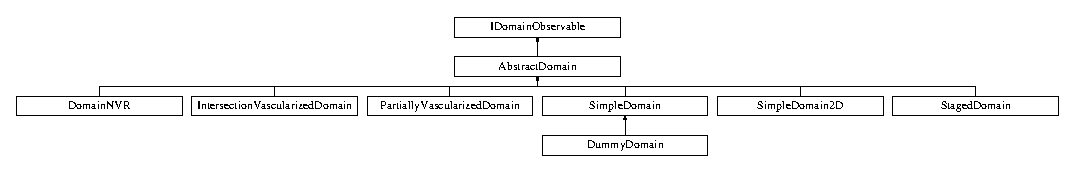
\includegraphics[height=1.857380cm]{d7/dc0/class_i_domain_observable}
\end{center}
\end{figure}
\subsection*{Public Member Functions}
\begin{DoxyCompactItemize}
\item 
\hyperlink{class_i_domain_observable_a4cd5c27295964fdc8acbe37898dd03b6}{I\+Domain\+Observable} ()
\item 
void \hyperlink{class_i_domain_observable_abe01724459dac9d6d72e5acbd676010b}{register\+Observer} (\hyperlink{class_i_domain_observer}{I\+Domain\+Observer} $\ast$observer)
\item 
void \hyperlink{class_i_domain_observable_a4ec3241ab4a686dd015518e0339db0f0}{notify\+Observers} ()
\end{DoxyCompactItemize}
\subsection*{Private Attributes}
\begin{DoxyCompactItemize}
\item 
vector$<$ \hyperlink{class_i_domain_observer}{I\+Domain\+Observer} $\ast$ $>$ \hyperlink{class_i_domain_observable_a0deaa551133a5b200a1127701440403d}{observers}
\end{DoxyCompactItemize}


\subsection{Detailed Description}
Observable class coplaint to observer/observable pattern. 

\subsection{Constructor \& Destructor Documentation}
\index{I\+Domain\+Observable@{I\+Domain\+Observable}!I\+Domain\+Observable@{I\+Domain\+Observable}}
\index{I\+Domain\+Observable@{I\+Domain\+Observable}!I\+Domain\+Observable@{I\+Domain\+Observable}}
\subsubsection[{\texorpdfstring{I\+Domain\+Observable()}{IDomainObservable()}}]{\setlength{\rightskip}{0pt plus 5cm}I\+Domain\+Observable\+::\+I\+Domain\+Observable (
\begin{DoxyParamCaption}
{}
\end{DoxyParamCaption}
)}\hypertarget{class_i_domain_observable_a4cd5c27295964fdc8acbe37898dd03b6}{}\label{class_i_domain_observable_a4cd5c27295964fdc8acbe37898dd03b6}
Constructor. 

\subsection{Member Function Documentation}
\index{I\+Domain\+Observable@{I\+Domain\+Observable}!notify\+Observers@{notify\+Observers}}
\index{notify\+Observers@{notify\+Observers}!I\+Domain\+Observable@{I\+Domain\+Observable}}
\subsubsection[{\texorpdfstring{notify\+Observers()}{notifyObservers()}}]{\setlength{\rightskip}{0pt plus 5cm}void I\+Domain\+Observable\+::notify\+Observers (
\begin{DoxyParamCaption}
{}
\end{DoxyParamCaption}
)}\hypertarget{class_i_domain_observable_a4ec3241ab4a686dd015518e0339db0f0}{}\label{class_i_domain_observable_a4ec3241ab4a686dd015518e0339db0f0}
Notify to all registrated observer executing the notified. \index{I\+Domain\+Observable@{I\+Domain\+Observable}!register\+Observer@{register\+Observer}}
\index{register\+Observer@{register\+Observer}!I\+Domain\+Observable@{I\+Domain\+Observable}}
\subsubsection[{\texorpdfstring{register\+Observer(\+I\+Domain\+Observer $\ast$observer)}{registerObserver(IDomainObserver *observer)}}]{\setlength{\rightskip}{0pt plus 5cm}void I\+Domain\+Observable\+::register\+Observer (
\begin{DoxyParamCaption}
\item[{{\bf I\+Domain\+Observer} $\ast$}]{observer}
\end{DoxyParamCaption}
)}\hypertarget{class_i_domain_observable_abe01724459dac9d6d72e5acbd676010b}{}\label{class_i_domain_observable_abe01724459dac9d6d72e5acbd676010b}
Registrate a new observer in order to notify each time that the observable class is updated. 
\begin{DoxyParams}{Parameters}
{\em observer} & Observer class type \hyperlink{class_i_domain_observer}{I\+Domain\+Observer}. \\
\hline
\end{DoxyParams}


\subsection{Member Data Documentation}
\index{I\+Domain\+Observable@{I\+Domain\+Observable}!observers@{observers}}
\index{observers@{observers}!I\+Domain\+Observable@{I\+Domain\+Observable}}
\subsubsection[{\texorpdfstring{observers}{observers}}]{\setlength{\rightskip}{0pt plus 5cm}vector$<${\bf I\+Domain\+Observer} $\ast$$>$ I\+Domain\+Observable\+::observers\hspace{0.3cm}{\ttfamily [private]}}\hypertarget{class_i_domain_observable_a0deaa551133a5b200a1127701440403d}{}\label{class_i_domain_observable_a0deaa551133a5b200a1127701440403d}
List of observer objects. 

The documentation for this class was generated from the following files\+:\begin{DoxyCompactItemize}
\item 
structures/domain/I\+Domain\+Observable.\+h\item 
structures/domain/I\+Domain\+Observable.\+cpp\end{DoxyCompactItemize}

\hypertarget{class_i_domain_observer}{}\section{I\+Domain\+Observer Class Reference}
\label{class_i_domain_observer}\index{I\+Domain\+Observer@{I\+Domain\+Observer}}


{\ttfamily \#include $<$I\+Domain\+Observer.\+h$>$}

Inheritance diagram for I\+Domain\+Observer\+:\begin{figure}[H]
\begin{center}
\leavevmode
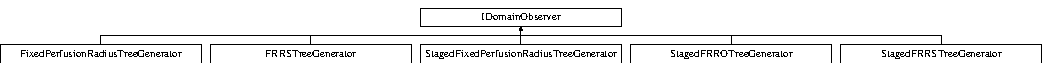
\includegraphics[height=0.845283cm]{d7/dc1/class_i_domain_observer}
\end{center}
\end{figure}
\subsection*{Public Member Functions}
\begin{DoxyCompactItemize}
\item 
\hyperlink{class_i_domain_observer_aeb993d11e1f33c0f22ad49bfee98253e}{I\+Domain\+Observer} ()
\item 
virtual void \hyperlink{class_i_domain_observer_aee18640c20a6feaa16e4bf3bdde887a3}{observable\+Modified} (\hyperlink{class_i_domain_observable}{I\+Domain\+Observable} $\ast$observable\+Instance)=0
\end{DoxyCompactItemize}


\subsection{Detailed Description}
Class that implements the observer end of an observer/observable pattern. Observable object will call observable\+Modified when its state changes. An observer object must register in the observable object in order to be called. 

\subsection{Constructor \& Destructor Documentation}
\index{I\+Domain\+Observer@{I\+Domain\+Observer}!I\+Domain\+Observer@{I\+Domain\+Observer}}
\index{I\+Domain\+Observer@{I\+Domain\+Observer}!I\+Domain\+Observer@{I\+Domain\+Observer}}
\subsubsection[{\texorpdfstring{I\+Domain\+Observer()}{IDomainObserver()}}]{\setlength{\rightskip}{0pt plus 5cm}I\+Domain\+Observer\+::\+I\+Domain\+Observer (
\begin{DoxyParamCaption}
{}
\end{DoxyParamCaption}
)}\hypertarget{class_i_domain_observer_aeb993d11e1f33c0f22ad49bfee98253e}{}\label{class_i_domain_observer_aeb993d11e1f33c0f22ad49bfee98253e}
Constructor 

\subsection{Member Function Documentation}
\index{I\+Domain\+Observer@{I\+Domain\+Observer}!observable\+Modified@{observable\+Modified}}
\index{observable\+Modified@{observable\+Modified}!I\+Domain\+Observer@{I\+Domain\+Observer}}
\subsubsection[{\texorpdfstring{observable\+Modified(\+I\+Domain\+Observable $\ast$observable\+Instance)=0}{observableModified(IDomainObservable *observableInstance)=0}}]{\setlength{\rightskip}{0pt plus 5cm}virtual void I\+Domain\+Observer\+::observable\+Modified (
\begin{DoxyParamCaption}
\item[{{\bf I\+Domain\+Observable} $\ast$}]{observable\+Instance}
\end{DoxyParamCaption}
)\hspace{0.3cm}{\ttfamily [pure virtual]}}\hypertarget{class_i_domain_observer_aee18640c20a6feaa16e4bf3bdde887a3}{}\label{class_i_domain_observer_aee18640c20a6feaa16e4bf3bdde887a3}
Method executed when {\ttfamily modified\+Domain} has changed. 
\begin{DoxyParams}{Parameters}
{\em observable\+Instance} & Observable domain. \\
\hline
\end{DoxyParams}


Implemented in \hyperlink{class_staged_fixed_perfusion_radius_tree_generator_a344e071b8da2eea979efdbdeb650a2a6}{Staged\+Fixed\+Perfusion\+Radius\+Tree\+Generator}, \hyperlink{class_staged_f_r_r_s_tree_generator_a6f7629b00510e27edddced056e6fa1a1}{Staged\+F\+R\+R\+S\+Tree\+Generator}, \hyperlink{class_fixed_perfusion_radius_tree_generator_add5bd06f4fe8a15529084f6d78e71b44}{Fixed\+Perfusion\+Radius\+Tree\+Generator}, \hyperlink{class_f_r_r_s_tree_generator_a4cde56db66ba928599c0ce263246c61e}{F\+R\+R\+S\+Tree\+Generator}, and \hyperlink{class_staged_f_r_r_o_tree_generator_a01a80f2720de4fe42b47dd9eb98a25bd}{Staged\+F\+R\+R\+O\+Tree\+Generator}.



The documentation for this class was generated from the following files\+:\begin{DoxyCompactItemize}
\item 
structures/domain/I\+Domain\+Observer.\+h\item 
structures/domain/I\+Domain\+Observer.\+cpp\end{DoxyCompactItemize}

\hypertarget{class_intersection_vascularized_domain}{}\section{Intersection\+Vascularized\+Domain Class Reference}
\label{class_intersection_vascularized_domain}\index{Intersection\+Vascularized\+Domain@{Intersection\+Vascularized\+Domain}}


{\ttfamily \#include $<$Intersection\+Vascularized\+Domain.\+h$>$}

Inheritance diagram for Intersection\+Vascularized\+Domain\+:\begin{figure}[H]
\begin{center}
\leavevmode
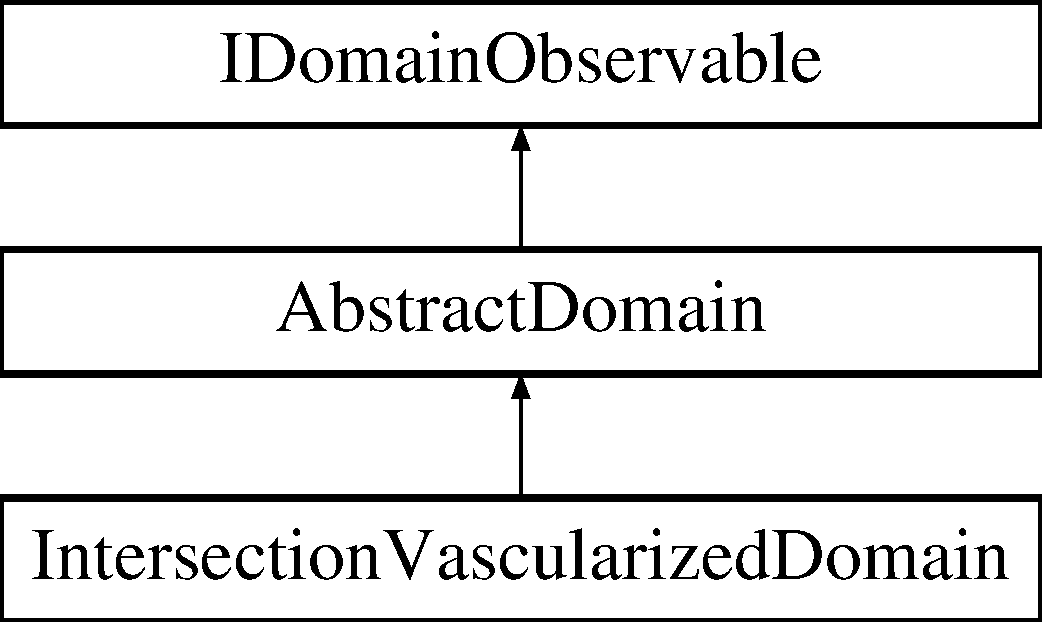
\includegraphics[height=3.000000cm]{d0/d59/class_intersection_vascularized_domain}
\end{center}
\end{figure}
\subsection*{Public Member Functions}
\begin{DoxyCompactItemize}
\item 
\hyperlink{class_intersection_vascularized_domain_ad5eb56a0c6f7197af3d1263f7625bbc5}{Intersection\+Vascularized\+Domain} (vector$<$ string $>$ filename\+Vascular\+Regions, \hyperlink{class_generator_data}{Generator\+Data} $\ast$\hyperlink{class_abstract_domain_aa37fbabc2bfa92c574f7db7544016b53}{instance\+Data})
\item 
\hyperlink{class_intersection_vascularized_domain_a5bd62b749b6f25562b7170e3bfb8f6d7}{Intersection\+Vascularized\+Domain} (vector$<$ string $>$ filename\+Vascular\+Regions, int \hyperlink{class_intersection_vascularized_domain_a98a16d98d16b37b13593d7a2aee872f3}{n\+Draw}, \hyperlink{class_generator_data}{Generator\+Data} $\ast$\hyperlink{class_abstract_domain_aa37fbabc2bfa92c574f7db7544016b53}{instance\+Data})
\item 
\hyperlink{class_intersection_vascularized_domain_a5b6f8a4f0c2a4eac2ba76dc3345a0994}{Intersection\+Vascularized\+Domain} (vector$<$ string $>$ filename\+Vascular\+Regions, int \hyperlink{class_intersection_vascularized_domain_a98a16d98d16b37b13593d7a2aee872f3}{n\+Draw}, int \hyperlink{class_intersection_vascularized_domain_abe078f4d223d21554d6f6709d5db47b0}{seed}, \hyperlink{class_generator_data}{Generator\+Data} $\ast$\hyperlink{class_abstract_domain_aa37fbabc2bfa92c574f7db7544016b53}{instance\+Data})
\item 
int \hyperlink{class_intersection_vascularized_domain_accd160eb77fede65322d67293177e54f}{is\+Segment\+Inside} (\hyperlink{structpoint}{point} xs, \hyperlink{structpoint}{point} xf)
\item 
double \hyperlink{class_intersection_vascularized_domain_a6ded581a637a098d2ddfec6ae6801132}{get\+Characteristic\+Length} ()
\item 
double \hyperlink{class_intersection_vascularized_domain_a24e31c45b099a27ea3d13b1923ea5340}{get\+D\+Lim} (long long int n\+Vessels, double factor)
\item 
double $\ast$ \hyperlink{class_intersection_vascularized_domain_a4b35793edb3ec9847e8be75d81dfbd9d}{get\+Local\+Neighborhood} (\hyperlink{structpoint}{point} p, long long int n\+Vessels)
\item 
double \hyperlink{class_intersection_vascularized_domain_a4c4dc6ce4711752e7d082346499d70b5}{get\+Size} ()
\item 
virtual \hyperlink{structpoint}{point} \hyperlink{class_intersection_vascularized_domain_a39e0fd3443fed3fecf4ecc799e39baa2}{get\+Random\+Point} ()
\item 
vtk\+Smart\+Pointer$<$ vtk\+O\+B\+B\+Tree $>$ \& \hyperlink{class_intersection_vascularized_domain_a1188cff5b710e8281a9cecf998532a20}{get\+Locator} ()
\item 
int \hyperlink{class_intersection_vascularized_domain_a451cea01fadfed6f9a1118755c36f16b}{get\+Draw} ()
\item 
deque$<$ \hyperlink{structpoint}{point} $>$ \& \hyperlink{class_intersection_vascularized_domain_afa0103c0c3ed989e1b67e50d14684321}{get\+Random\+Inner\+Points} ()
\item 
vtk\+Smart\+Pointer$<$ vtk\+Poly\+Data $>$ \& \hyperlink{class_intersection_vascularized_domain_aacdc4a4263423e8c8dd992ba4f00f826}{get\+Vtk\+Geometry} ()
\end{DoxyCompactItemize}
\subsection*{Protected Member Functions}
\begin{DoxyCompactItemize}
\item 
void {\bfseries generate\+Random\+Points} ()\hypertarget{class_intersection_vascularized_domain_a9f49c20ae3e45f5c3a45d95c7a83f564}{}\label{class_intersection_vascularized_domain_a9f49c20ae3e45f5c3a45d95c7a83f564}

\item 
void {\bfseries remove\+Random\+Outer\+Points} ()\hypertarget{class_intersection_vascularized_domain_a835ac8aeef4b5c2731ca8b0f2c36e727}{}\label{class_intersection_vascularized_domain_a835ac8aeef4b5c2731ca8b0f2c36e727}

\end{DoxyCompactItemize}
\subsection*{Protected Attributes}
\begin{DoxyCompactItemize}
\item 
deque$<$ \hyperlink{structpoint}{point} $>$ {\bfseries random\+Inner\+Points}\hypertarget{class_intersection_vascularized_domain_afdb89cfb5da3abb20351ece21dc500d0}{}\label{class_intersection_vascularized_domain_afdb89cfb5da3abb20351ece21dc500d0}

\end{DoxyCompactItemize}
\subsection*{Private Attributes}
\begin{DoxyCompactItemize}
\item 
vector$<$ vtk\+Smart\+Pointer$<$ vtk\+Poly\+Data $>$ $>$ \hyperlink{class_intersection_vascularized_domain_a0cfc67dad7db0d7c95b50eb6992c8339}{vtk\+Vascularized\+Regions}
\item 
vector$<$ vtk\+Smart\+Pointer$<$ vtk\+O\+B\+B\+Tree $>$ $>$ \hyperlink{class_intersection_vascularized_domain_aedf9a331b6785010abad7111b447a418}{sublocators}
\item 
double $\ast$ \hyperlink{class_intersection_vascularized_domain_a09393f0750ed293a45953f3a080cd7d6}{bounding\+Box}
\item 
double \hyperlink{class_intersection_vascularized_domain_a6cd023b45323ac979b45ff56597ad621}{characteristic\+Length}
\item 
int \hyperlink{class_intersection_vascularized_domain_a98a16d98d16b37b13593d7a2aee872f3}{n\+Draw}
\item 
int \hyperlink{class_intersection_vascularized_domain_abe078f4d223d21554d6f6709d5db47b0}{seed} = -\/1
\item 
mt19937 \hyperlink{class_intersection_vascularized_domain_a6245d7a96b0c7e453080ccde826ea654}{generator}
\end{DoxyCompactItemize}


\subsection{Detailed Description}
This domain vascularises just the intersection between all vascularised regions. 

\subsection{Constructor \& Destructor Documentation}
\index{Intersection\+Vascularized\+Domain@{Intersection\+Vascularized\+Domain}!Intersection\+Vascularized\+Domain@{Intersection\+Vascularized\+Domain}}
\index{Intersection\+Vascularized\+Domain@{Intersection\+Vascularized\+Domain}!Intersection\+Vascularized\+Domain@{Intersection\+Vascularized\+Domain}}
\subsubsection[{\texorpdfstring{Intersection\+Vascularized\+Domain(vector$<$ string $>$ filename\+Vascular\+Regions, Generator\+Data $\ast$instance\+Data)}{IntersectionVascularizedDomain(vector< string > filenameVascularRegions, GeneratorData *instanceData)}}]{\setlength{\rightskip}{0pt plus 5cm}Intersection\+Vascularized\+Domain\+::\+Intersection\+Vascularized\+Domain (
\begin{DoxyParamCaption}
\item[{vector$<$ string $>$}]{filename\+Vascular\+Regions, }
\item[{{\bf Generator\+Data} $\ast$}]{instance\+Data}
\end{DoxyParamCaption}
)}\hypertarget{class_intersection_vascularized_domain_ad5eb56a0c6f7197af3d1263f7625bbc5}{}\label{class_intersection_vascularized_domain_ad5eb56a0c6f7197af3d1263f7625bbc5}
Constructs a domain shaped by {\ttfamily filename\+Hull} (transport domain) with vascularized and non-\/vascularized regions contained in {\ttfamily filename\+Vascular\+Regions} and {\ttfamily filename\+Non\+Vascular\+Regions} respectively. 
\begin{DoxyParams}{Parameters}
{\em filename\+Hull} & Domain description. \\
\hline
{\em filename\+Vascular\+Regions} & Vascularized regions descriptions. \\
\hline
{\em filename\+Non\+Vascular\+Regions} & Non-\/vascularized regions descriptions. \\
\hline
\end{DoxyParams}
\index{Intersection\+Vascularized\+Domain@{Intersection\+Vascularized\+Domain}!Intersection\+Vascularized\+Domain@{Intersection\+Vascularized\+Domain}}
\index{Intersection\+Vascularized\+Domain@{Intersection\+Vascularized\+Domain}!Intersection\+Vascularized\+Domain@{Intersection\+Vascularized\+Domain}}
\subsubsection[{\texorpdfstring{Intersection\+Vascularized\+Domain(vector$<$ string $>$ filename\+Vascular\+Regions, int n\+Draw, Generator\+Data $\ast$instance\+Data)}{IntersectionVascularizedDomain(vector< string > filenameVascularRegions, int nDraw, GeneratorData *instanceData)}}]{\setlength{\rightskip}{0pt plus 5cm}Intersection\+Vascularized\+Domain\+::\+Intersection\+Vascularized\+Domain (
\begin{DoxyParamCaption}
\item[{vector$<$ string $>$}]{filename\+Vascular\+Regions, }
\item[{int}]{n\+Draw, }
\item[{{\bf Generator\+Data} $\ast$}]{instance\+Data}
\end{DoxyParamCaption}
)}\hypertarget{class_intersection_vascularized_domain_a5bd62b749b6f25562b7170e3bfb8f6d7}{}\label{class_intersection_vascularized_domain_a5bd62b749b6f25562b7170e3bfb8f6d7}
Constructs a domain shaped by {\ttfamily filename\+Hull} (transport domain) with vascularized and non-\/vascularized regions contained in {\ttfamily filename\+Vascular\+Regions} and {\ttfamily filename\+Non\+Vascular\+Regions} respectively. Also, itgenerates batches of {\ttfamily n\+Draw} random points each time that the domain is with no more points. 
\begin{DoxyParams}{Parameters}
{\em filename\+Vascular\+Regions} & Vascularized regions descriptions. \\
\hline
{\em n\+Draw} & Random points generated at each batch. \\
\hline
\end{DoxyParams}
\index{Intersection\+Vascularized\+Domain@{Intersection\+Vascularized\+Domain}!Intersection\+Vascularized\+Domain@{Intersection\+Vascularized\+Domain}}
\index{Intersection\+Vascularized\+Domain@{Intersection\+Vascularized\+Domain}!Intersection\+Vascularized\+Domain@{Intersection\+Vascularized\+Domain}}
\subsubsection[{\texorpdfstring{Intersection\+Vascularized\+Domain(vector$<$ string $>$ filename\+Vascular\+Regions, int n\+Draw, int seed, Generator\+Data $\ast$instance\+Data)}{IntersectionVascularizedDomain(vector< string > filenameVascularRegions, int nDraw, int seed, GeneratorData *instanceData)}}]{\setlength{\rightskip}{0pt plus 5cm}Intersection\+Vascularized\+Domain\+::\+Intersection\+Vascularized\+Domain (
\begin{DoxyParamCaption}
\item[{vector$<$ string $>$}]{filename\+Vascular\+Regions, }
\item[{int}]{n\+Draw, }
\item[{int}]{seed, }
\item[{{\bf Generator\+Data} $\ast$}]{instance\+Data}
\end{DoxyParamCaption}
)}\hypertarget{class_intersection_vascularized_domain_a5b6f8a4f0c2a4eac2ba76dc3345a0994}{}\label{class_intersection_vascularized_domain_a5b6f8a4f0c2a4eac2ba76dc3345a0994}
Constructs a domain shaped by {\ttfamily filename\+Hull} (transport domain) with vascularized and non-\/vascularized regions contained in {\ttfamily filename\+Vascular\+Regions} and {\ttfamily filename\+Non\+Vascular\+Regions} respectively. Also, itgenerates batches of {\ttfamily n\+Draw} random points each time that the domain is with no more points. 
\begin{DoxyParams}{Parameters}
{\em filename\+Vascular\+Regions} & Vascularized regions descriptions. \\
\hline
{\em n\+Draw} & Random points generated at each batch. \\
\hline
{\em seed} & Seed for random points generation. \\
\hline
\end{DoxyParams}


\subsection{Member Function Documentation}
\index{Intersection\+Vascularized\+Domain@{Intersection\+Vascularized\+Domain}!get\+Characteristic\+Length@{get\+Characteristic\+Length}}
\index{get\+Characteristic\+Length@{get\+Characteristic\+Length}!Intersection\+Vascularized\+Domain@{Intersection\+Vascularized\+Domain}}
\subsubsection[{\texorpdfstring{get\+Characteristic\+Length()}{getCharacteristicLength()}}]{\setlength{\rightskip}{0pt plus 5cm}double Intersection\+Vascularized\+Domain\+::get\+Characteristic\+Length (
\begin{DoxyParamCaption}
{}
\end{DoxyParamCaption}
)\hspace{0.3cm}{\ttfamily [virtual]}}\hypertarget{class_intersection_vascularized_domain_a6ded581a637a098d2ddfec6ae6801132}{}\label{class_intersection_vascularized_domain_a6ded581a637a098d2ddfec6ae6801132}
Estimates a characteristic length for the current domain. This length is useful to estimate the perfusion volume of the domain. \begin{DoxyReturn}{Returns}
Chracteristic length. 
\end{DoxyReturn}


Implements \hyperlink{class_abstract_domain_a90ca3dff64bab2428da8ced24e16f4c3}{Abstract\+Domain}.

\index{Intersection\+Vascularized\+Domain@{Intersection\+Vascularized\+Domain}!get\+D\+Lim@{get\+D\+Lim}}
\index{get\+D\+Lim@{get\+D\+Lim}!Intersection\+Vascularized\+Domain@{Intersection\+Vascularized\+Domain}}
\subsubsection[{\texorpdfstring{get\+D\+Lim(long long int n\+Vessels, double factor)}{getDLim(long long int nVessels, double factor)}}]{\setlength{\rightskip}{0pt plus 5cm}double Intersection\+Vascularized\+Domain\+::get\+D\+Lim (
\begin{DoxyParamCaption}
\item[{long long int}]{n\+Vessels, }
\item[{double}]{factor}
\end{DoxyParamCaption}
)\hspace{0.3cm}{\ttfamily [virtual]}}\hypertarget{class_intersection_vascularized_domain_a24e31c45b099a27ea3d13b1923ea5340}{}\label{class_intersection_vascularized_domain_a24e31c45b099a27ea3d13b1923ea5340}
Minimum distance between a new vessel terminal and the tree based on the current terminal perfusion. This is lower bound criteria for the vessel length and also aids toward a spatially homogeneous terminal distribution. 
\begin{DoxyParams}{Parameters}
{\em n\+Vessels} & Quantity of terminals in the current tree. \\
\hline
{\em factor} & Factor used to scale a perfusion measure in order to estimate the D\+Lim value. \\
\hline
\end{DoxyParams}
\begin{DoxyReturn}{Returns}
D\+Lim value. 
\end{DoxyReturn}


Implements \hyperlink{class_abstract_domain_ac9f39c12182608eb704c051e5d1cbc55}{Abstract\+Domain}.

\index{Intersection\+Vascularized\+Domain@{Intersection\+Vascularized\+Domain}!get\+Draw@{get\+Draw}}
\index{get\+Draw@{get\+Draw}!Intersection\+Vascularized\+Domain@{Intersection\+Vascularized\+Domain}}
\subsubsection[{\texorpdfstring{get\+Draw()}{getDraw()}}]{\setlength{\rightskip}{0pt plus 5cm}int Intersection\+Vascularized\+Domain\+::get\+Draw (
\begin{DoxyParamCaption}
{}
\end{DoxyParamCaption}
)}\hypertarget{class_intersection_vascularized_domain_a451cea01fadfed6f9a1118755c36f16b}{}\label{class_intersection_vascularized_domain_a451cea01fadfed6f9a1118755c36f16b}
Returns the number of random points created in each batch of random generations. \begin{DoxyReturn}{Returns}
Number of random points created in each batch of random generations. 
\end{DoxyReturn}
\index{Intersection\+Vascularized\+Domain@{Intersection\+Vascularized\+Domain}!get\+Local\+Neighborhood@{get\+Local\+Neighborhood}}
\index{get\+Local\+Neighborhood@{get\+Local\+Neighborhood}!Intersection\+Vascularized\+Domain@{Intersection\+Vascularized\+Domain}}
\subsubsection[{\texorpdfstring{get\+Local\+Neighborhood(point p, long long int n\+Vessels)}{getLocalNeighborhood(point p, long long int nVessels)}}]{\setlength{\rightskip}{0pt plus 5cm}double $\ast$ Intersection\+Vascularized\+Domain\+::get\+Local\+Neighborhood (
\begin{DoxyParamCaption}
\item[{{\bf point}}]{p, }
\item[{long long int}]{n\+Vessels}
\end{DoxyParamCaption}
)\hspace{0.3cm}{\ttfamily [virtual]}}\hypertarget{class_intersection_vascularized_domain_a4b35793edb3ec9847e8be75d81dfbd9d}{}\label{class_intersection_vascularized_domain_a4b35793edb3ec9847e8be75d81dfbd9d}
Returns the local neighbors to the {\ttfamily p} point locus. The amount of neighbors is estimated based on the current terminal perfusion. 
\begin{DoxyParams}{Parameters}
{\em p} & Central point of the neighborhood. \\
\hline
{\em n\+Vessels} & Amount of terminals in the tree. \\
\hline
\end{DoxyParams}
\begin{DoxyReturn}{Returns}
Array of neighbor vessels. 
\end{DoxyReturn}


Implements \hyperlink{class_abstract_domain_aee2b549d19062b261429f8a442fb4714}{Abstract\+Domain}.

\index{Intersection\+Vascularized\+Domain@{Intersection\+Vascularized\+Domain}!get\+Locator@{get\+Locator}}
\index{get\+Locator@{get\+Locator}!Intersection\+Vascularized\+Domain@{Intersection\+Vascularized\+Domain}}
\subsubsection[{\texorpdfstring{get\+Locator()}{getLocator()}}]{\setlength{\rightskip}{0pt plus 5cm}vtk\+Smart\+Pointer$<$ vtk\+O\+B\+B\+Tree $>$ \& Intersection\+Vascularized\+Domain\+::get\+Locator (
\begin{DoxyParamCaption}
{}
\end{DoxyParamCaption}
)}\hypertarget{class_intersection_vascularized_domain_a1188cff5b710e8281a9cecf998532a20}{}\label{class_intersection_vascularized_domain_a1188cff5b710e8281a9cecf998532a20}
Returns the locator used to test inside segments. \begin{DoxyReturn}{Returns}
Locator used to test inside segments. 
\end{DoxyReturn}
\index{Intersection\+Vascularized\+Domain@{Intersection\+Vascularized\+Domain}!get\+Random\+Inner\+Points@{get\+Random\+Inner\+Points}}
\index{get\+Random\+Inner\+Points@{get\+Random\+Inner\+Points}!Intersection\+Vascularized\+Domain@{Intersection\+Vascularized\+Domain}}
\subsubsection[{\texorpdfstring{get\+Random\+Inner\+Points()}{getRandomInnerPoints()}}]{\setlength{\rightskip}{0pt plus 5cm}deque$<$ {\bf point} $>$ \& Intersection\+Vascularized\+Domain\+::get\+Random\+Inner\+Points (
\begin{DoxyParamCaption}
{}
\end{DoxyParamCaption}
)\hspace{0.3cm}{\ttfamily [virtual]}}\hypertarget{class_intersection_vascularized_domain_afa0103c0c3ed989e1b67e50d14684321}{}\label{class_intersection_vascularized_domain_afa0103c0c3ed989e1b67e50d14684321}
Return a set of inner domain points. \begin{DoxyReturn}{Returns}
Set of inner domain points. 
\end{DoxyReturn}


Implements \hyperlink{class_abstract_domain_a73d2c0e7c670b007bb5dbbdab5ad6b1b}{Abstract\+Domain}.

\index{Intersection\+Vascularized\+Domain@{Intersection\+Vascularized\+Domain}!get\+Random\+Point@{get\+Random\+Point}}
\index{get\+Random\+Point@{get\+Random\+Point}!Intersection\+Vascularized\+Domain@{Intersection\+Vascularized\+Domain}}
\subsubsection[{\texorpdfstring{get\+Random\+Point()}{getRandomPoint()}}]{\setlength{\rightskip}{0pt plus 5cm}{\bf point} Intersection\+Vascularized\+Domain\+::get\+Random\+Point (
\begin{DoxyParamCaption}
{}
\end{DoxyParamCaption}
)\hspace{0.3cm}{\ttfamily [virtual]}}\hypertarget{class_intersection_vascularized_domain_a39e0fd3443fed3fecf4ecc799e39baa2}{}\label{class_intersection_vascularized_domain_a39e0fd3443fed3fecf4ecc799e39baa2}
Return a random point inside the domain. \begin{DoxyReturn}{Returns}
Point inside the domain. 
\end{DoxyReturn}


Implements \hyperlink{class_abstract_domain_ae31a5b26d1dc628abe24da7a4d375415}{Abstract\+Domain}.

\index{Intersection\+Vascularized\+Domain@{Intersection\+Vascularized\+Domain}!get\+Size@{get\+Size}}
\index{get\+Size@{get\+Size}!Intersection\+Vascularized\+Domain@{Intersection\+Vascularized\+Domain}}
\subsubsection[{\texorpdfstring{get\+Size()}{getSize()}}]{\setlength{\rightskip}{0pt plus 5cm}double Intersection\+Vascularized\+Domain\+::get\+Size (
\begin{DoxyParamCaption}
{}
\end{DoxyParamCaption}
)\hspace{0.3cm}{\ttfamily [virtual]}}\hypertarget{class_intersection_vascularized_domain_a4c4dc6ce4711752e7d082346499d70b5}{}\label{class_intersection_vascularized_domain_a4c4dc6ce4711752e7d082346499d70b5}
Computes the size of the domain. \begin{DoxyReturn}{Returns}
Size of the domain. 
\end{DoxyReturn}


Implements \hyperlink{class_abstract_domain_a049564d82f2c177c39834dfc8da143dc}{Abstract\+Domain}.

\index{Intersection\+Vascularized\+Domain@{Intersection\+Vascularized\+Domain}!get\+Vtk\+Geometry@{get\+Vtk\+Geometry}}
\index{get\+Vtk\+Geometry@{get\+Vtk\+Geometry}!Intersection\+Vascularized\+Domain@{Intersection\+Vascularized\+Domain}}
\subsubsection[{\texorpdfstring{get\+Vtk\+Geometry()}{getVtkGeometry()}}]{\setlength{\rightskip}{0pt plus 5cm}vtk\+Smart\+Pointer$<$ vtk\+Poly\+Data $>$ \& Intersection\+Vascularized\+Domain\+::get\+Vtk\+Geometry (
\begin{DoxyParamCaption}
{}
\end{DoxyParamCaption}
)\hspace{0.3cm}{\ttfamily [virtual]}}\hypertarget{class_intersection_vascularized_domain_aacdc4a4263423e8c8dd992ba4f00f826}{}\label{class_intersection_vascularized_domain_aacdc4a4263423e8c8dd992ba4f00f826}
Returns the vtk\+Polydata with the domain representation. \begin{DoxyReturn}{Returns}
vtk\+Polydata with the domain representation. 
\end{DoxyReturn}


Implements \hyperlink{class_abstract_domain_abb1e386d2899cb6b725509259a836cd0}{Abstract\+Domain}.

\index{Intersection\+Vascularized\+Domain@{Intersection\+Vascularized\+Domain}!is\+Segment\+Inside@{is\+Segment\+Inside}}
\index{is\+Segment\+Inside@{is\+Segment\+Inside}!Intersection\+Vascularized\+Domain@{Intersection\+Vascularized\+Domain}}
\subsubsection[{\texorpdfstring{is\+Segment\+Inside(point xs, point xf)}{isSegmentInside(point xs, point xf)}}]{\setlength{\rightskip}{0pt plus 5cm}int Intersection\+Vascularized\+Domain\+::is\+Segment\+Inside (
\begin{DoxyParamCaption}
\item[{{\bf point}}]{xs, }
\item[{{\bf point}}]{xf}
\end{DoxyParamCaption}
)\hspace{0.3cm}{\ttfamily [virtual]}}\hypertarget{class_intersection_vascularized_domain_accd160eb77fede65322d67293177e54f}{}\label{class_intersection_vascularized_domain_accd160eb77fede65322d67293177e54f}
Returns if the segment defined by the vertexes {\ttfamily xs} and {\ttfamily xf} is inside the current transport domain without intersecting non-\/vascularized regions. 
\begin{DoxyParams}{Parameters}
{\em xs} & Start point of the segment. \\
\hline
{\em xf} & End point of the segment. \\
\hline
\end{DoxyParams}
\begin{DoxyReturn}{Returns}
1 if the segment defined by the vertexes {\ttfamily xs} and {\ttfamily xf} is inside the current domain otherwise 0. 
\end{DoxyReturn}


Implements \hyperlink{class_abstract_domain_a8544eef21fb6700ecc02e9cd50884efd}{Abstract\+Domain}.



\subsection{Member Data Documentation}
\index{Intersection\+Vascularized\+Domain@{Intersection\+Vascularized\+Domain}!bounding\+Box@{bounding\+Box}}
\index{bounding\+Box@{bounding\+Box}!Intersection\+Vascularized\+Domain@{Intersection\+Vascularized\+Domain}}
\subsubsection[{\texorpdfstring{bounding\+Box}{boundingBox}}]{\setlength{\rightskip}{0pt plus 5cm}double$\ast$ Intersection\+Vascularized\+Domain\+::bounding\+Box\hspace{0.3cm}{\ttfamily [private]}}\hypertarget{class_intersection_vascularized_domain_a09393f0750ed293a45953f3a080cd7d6}{}\label{class_intersection_vascularized_domain_a09393f0750ed293a45953f3a080cd7d6}
Bounding box of the domain \index{Intersection\+Vascularized\+Domain@{Intersection\+Vascularized\+Domain}!characteristic\+Length@{characteristic\+Length}}
\index{characteristic\+Length@{characteristic\+Length}!Intersection\+Vascularized\+Domain@{Intersection\+Vascularized\+Domain}}
\subsubsection[{\texorpdfstring{characteristic\+Length}{characteristicLength}}]{\setlength{\rightskip}{0pt plus 5cm}double Intersection\+Vascularized\+Domain\+::characteristic\+Length\hspace{0.3cm}{\ttfamily [private]}}\hypertarget{class_intersection_vascularized_domain_a6cd023b45323ac979b45ff56597ad621}{}\label{class_intersection_vascularized_domain_a6cd023b45323ac979b45ff56597ad621}
Characteristic length for the domain. \index{Intersection\+Vascularized\+Domain@{Intersection\+Vascularized\+Domain}!generator@{generator}}
\index{generator@{generator}!Intersection\+Vascularized\+Domain@{Intersection\+Vascularized\+Domain}}
\subsubsection[{\texorpdfstring{generator}{generator}}]{\setlength{\rightskip}{0pt plus 5cm}mt19937 Intersection\+Vascularized\+Domain\+::generator\hspace{0.3cm}{\ttfamily [private]}}\hypertarget{class_intersection_vascularized_domain_a6245d7a96b0c7e453080ccde826ea654}{}\label{class_intersection_vascularized_domain_a6245d7a96b0c7e453080ccde826ea654}
Random generator. \index{Intersection\+Vascularized\+Domain@{Intersection\+Vascularized\+Domain}!n\+Draw@{n\+Draw}}
\index{n\+Draw@{n\+Draw}!Intersection\+Vascularized\+Domain@{Intersection\+Vascularized\+Domain}}
\subsubsection[{\texorpdfstring{n\+Draw}{nDraw}}]{\setlength{\rightskip}{0pt plus 5cm}int Intersection\+Vascularized\+Domain\+::n\+Draw\hspace{0.3cm}{\ttfamily [private]}}\hypertarget{class_intersection_vascularized_domain_a98a16d98d16b37b13593d7a2aee872f3}{}\label{class_intersection_vascularized_domain_a98a16d98d16b37b13593d7a2aee872f3}
Amount of points randomly generated when no more points are available. \index{Intersection\+Vascularized\+Domain@{Intersection\+Vascularized\+Domain}!seed@{seed}}
\index{seed@{seed}!Intersection\+Vascularized\+Domain@{Intersection\+Vascularized\+Domain}}
\subsubsection[{\texorpdfstring{seed}{seed}}]{\setlength{\rightskip}{0pt plus 5cm}int Intersection\+Vascularized\+Domain\+::seed = -\/1\hspace{0.3cm}{\ttfamily [private]}}\hypertarget{class_intersection_vascularized_domain_abe078f4d223d21554d6f6709d5db47b0}{}\label{class_intersection_vascularized_domain_abe078f4d223d21554d6f6709d5db47b0}
Random instance seed. \index{Intersection\+Vascularized\+Domain@{Intersection\+Vascularized\+Domain}!sublocators@{sublocators}}
\index{sublocators@{sublocators}!Intersection\+Vascularized\+Domain@{Intersection\+Vascularized\+Domain}}
\subsubsection[{\texorpdfstring{sublocators}{sublocators}}]{\setlength{\rightskip}{0pt plus 5cm}vector$<$vtk\+Smart\+Pointer$<$vtk\+O\+B\+B\+Tree$>$ $>$ Intersection\+Vascularized\+Domain\+::sublocators\hspace{0.3cm}{\ttfamily [private]}}\hypertarget{class_intersection_vascularized_domain_aedf9a331b6785010abad7111b447a418}{}\label{class_intersection_vascularized_domain_aedf9a331b6785010abad7111b447a418}
Cell locators responsible to determine if a segment is inside of each domain. \index{Intersection\+Vascularized\+Domain@{Intersection\+Vascularized\+Domain}!vtk\+Vascularized\+Regions@{vtk\+Vascularized\+Regions}}
\index{vtk\+Vascularized\+Regions@{vtk\+Vascularized\+Regions}!Intersection\+Vascularized\+Domain@{Intersection\+Vascularized\+Domain}}
\subsubsection[{\texorpdfstring{vtk\+Vascularized\+Regions}{vtkVascularizedRegions}}]{\setlength{\rightskip}{0pt plus 5cm}vector$<$vtk\+Smart\+Pointer$<$vtk\+Poly\+Data$>$ $>$ Intersection\+Vascularized\+Domain\+::vtk\+Vascularized\+Regions\hspace{0.3cm}{\ttfamily [private]}}\hypertarget{class_intersection_vascularized_domain_a0cfc67dad7db0d7c95b50eb6992c8339}{}\label{class_intersection_vascularized_domain_a0cfc67dad7db0d7c95b50eb6992c8339}
Vascularized subdomains represented by vtk\+Polydata. 

The documentation for this class was generated from the following files\+:\begin{DoxyCompactItemize}
\item 
structures/domain/Intersection\+Vascularized\+Domain.\+h\item 
structures/domain/Intersection\+Vascularized\+Domain.\+cpp\end{DoxyCompactItemize}

\hypertarget{class_mean_stat_manipulator}{}\section{Mean\+Stat\+Manipulator Class Reference}
\label{class_mean_stat_manipulator}\index{Mean\+Stat\+Manipulator@{Mean\+Stat\+Manipulator}}


{\ttfamily \#include $<$Mean\+Stat\+Manipulator.\+h$>$}

Inheritance diagram for Mean\+Stat\+Manipulator\+:\begin{figure}[H]
\begin{center}
\leavevmode
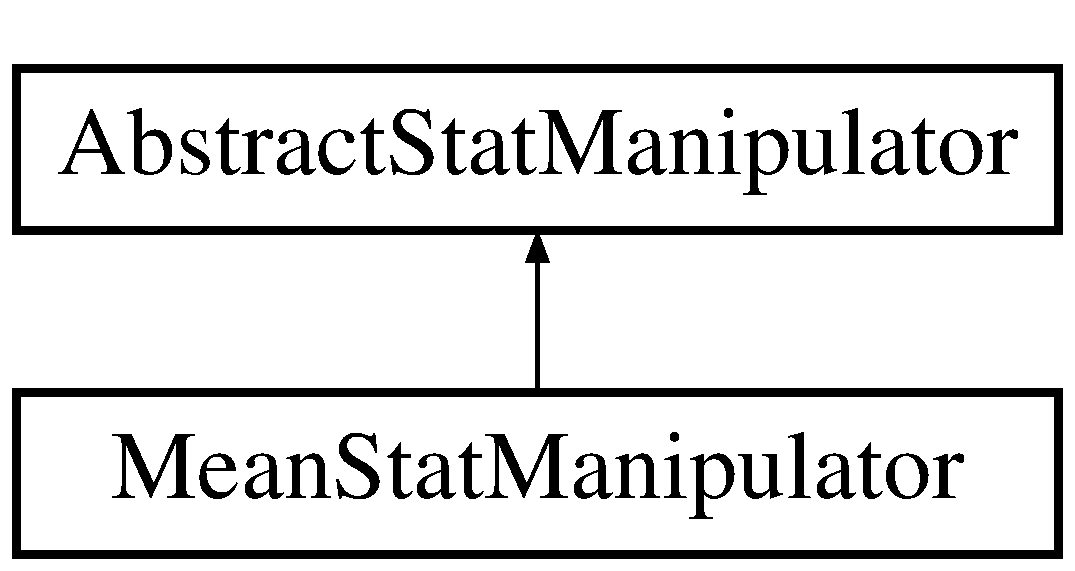
\includegraphics[height=2.000000cm]{d1/d8b/class_mean_stat_manipulator}
\end{center}
\end{figure}
\subsection*{Public Member Functions}
\begin{DoxyCompactItemize}
\item 
\hyperlink{class_mean_stat_manipulator_a9be1ad0a1ca9755c249ec11ca7f3f061}{Mean\+Stat\+Manipulator} ()
\item 
double \hyperlink{class_mean_stat_manipulator_ac5bfefb995b01bf06e39a694be3c0595}{compute} (vector$<$ \hyperlink{structvessel}{vessel} $\ast$ $>$ vessels, \hyperlink{class_vessel_handler_a6cc775e9a5bcbe69ef381f56b52982e7}{Vessel\+Handler\+::\+A\+T\+T\+R\+I\+B\+U\+TE} att)
\end{DoxyCompactItemize}
\subsection*{Additional Inherited Members}


\subsection{Detailed Description}
Computes the mean of a specific attribute for an array of vessels. 

\subsection{Constructor \& Destructor Documentation}
\index{Mean\+Stat\+Manipulator@{Mean\+Stat\+Manipulator}!Mean\+Stat\+Manipulator@{Mean\+Stat\+Manipulator}}
\index{Mean\+Stat\+Manipulator@{Mean\+Stat\+Manipulator}!Mean\+Stat\+Manipulator@{Mean\+Stat\+Manipulator}}
\subsubsection[{\texorpdfstring{Mean\+Stat\+Manipulator()}{MeanStatManipulator()}}]{\setlength{\rightskip}{0pt plus 5cm}Mean\+Stat\+Manipulator\+::\+Mean\+Stat\+Manipulator (
\begin{DoxyParamCaption}
{}
\end{DoxyParamCaption}
)}\hypertarget{class_mean_stat_manipulator_a9be1ad0a1ca9755c249ec11ca7f3f061}{}\label{class_mean_stat_manipulator_a9be1ad0a1ca9755c249ec11ca7f3f061}
Dummy constructor. 

\subsection{Member Function Documentation}
\index{Mean\+Stat\+Manipulator@{Mean\+Stat\+Manipulator}!compute@{compute}}
\index{compute@{compute}!Mean\+Stat\+Manipulator@{Mean\+Stat\+Manipulator}}
\subsubsection[{\texorpdfstring{compute(vector$<$ vessel $\ast$ $>$ vessels, Vessel\+Handler\+::\+A\+T\+T\+R\+I\+B\+U\+T\+E att)}{compute(vector< vessel * > vessels, VesselHandler::ATTRIBUTE att)}}]{\setlength{\rightskip}{0pt plus 5cm}double Mean\+Stat\+Manipulator\+::compute (
\begin{DoxyParamCaption}
\item[{vector$<$ {\bf vessel} $\ast$ $>$}]{vessels, }
\item[{{\bf Vessel\+Handler\+::\+A\+T\+T\+R\+I\+B\+U\+TE}}]{att}
\end{DoxyParamCaption}
)\hspace{0.3cm}{\ttfamily [virtual]}}\hypertarget{class_mean_stat_manipulator_ac5bfefb995b01bf06e39a694be3c0595}{}\label{class_mean_stat_manipulator_ac5bfefb995b01bf06e39a694be3c0595}
Computes the mean of the attribute of interest among all {\ttfamily vessels}. 
\begin{DoxyParams}{Parameters}
{\em vessels} & Array of vessels from which the statistical function is computed. \\
\hline
\end{DoxyParams}
\begin{DoxyReturn}{Returns}
Mean value. 
\end{DoxyReturn}


Implements \hyperlink{class_abstract_stat_manipulator_a8ae1dd190a2c85ff4e219a48f92763b7}{Abstract\+Stat\+Manipulator}.



The documentation for this class was generated from the following files\+:\begin{DoxyCompactItemize}
\item 
stats/Mean\+Stat\+Manipulator.\+h\item 
stats/Mean\+Stat\+Manipulator.\+cpp\end{DoxyCompactItemize}

\hypertarget{class_memory_monitor}{}\section{Memory\+Monitor Class Reference}
\label{class_memory_monitor}\index{Memory\+Monitor@{Memory\+Monitor}}


{\ttfamily \#include $<$Memory\+Monitor.\+h$>$}

\subsection*{Public Types}
\begin{DoxyCompactItemize}
\item 
enum \hyperlink{class_memory_monitor_aab7a81fc67c4acdf0d3c4ffefe3ef740}{U\+N\+I\+TS} \{ {\bfseries B\+Y\+TE}, 
{\bfseries K\+I\+L\+O\+B\+Y\+TE}, 
{\bfseries M\+E\+G\+A\+B\+Y\+TE}, 
{\bfseries G\+I\+G\+A\+B\+Y\+TE}
 \}
\end{DoxyCompactItemize}
\subsection*{Public Member Functions}
\begin{DoxyCompactItemize}
\item 
\hyperlink{class_memory_monitor_a03d307d8b56faf99571de9836a74fecf}{Memory\+Monitor} (\hyperlink{class_memory_monitor_aab7a81fc67c4acdf0d3c4ffefe3ef740}{U\+N\+I\+TS} unit)
\item 
long long \hyperlink{class_memory_monitor_ad5661e725b77131a188fb766987321a1}{get\+Process\+Memory\+Consumption} ()
\item 
long long \hyperlink{class_memory_monitor_a2b9ef8cb8113acdded0d6c3170e47cd2}{get\+System\+Memory\+Consumption} ()
\end{DoxyCompactItemize}
\subsection*{Private Member Functions}
\begin{DoxyCompactItemize}
\item 
int {\bfseries parse\+Line} (char $\ast$line)\hypertarget{class_memory_monitor_a3ed92d5612089f555f11e6a49e6f0e7c}{}\label{class_memory_monitor_a3ed92d5612089f555f11e6a49e6f0e7c}

\item 
long long {\bfseries get\+Value} ()\hypertarget{class_memory_monitor_a3311171846147b7c2d4bf2e2253b6db9}{}\label{class_memory_monitor_a3311171846147b7c2d4bf2e2253b6db9}

\end{DoxyCompactItemize}
\subsection*{Private Attributes}
\begin{DoxyCompactItemize}
\item 
double \hyperlink{class_memory_monitor_af9a6afbcc1408ffacbe85747ae9cea48}{unit\+Factor}
\end{DoxyCompactItemize}


\subsection{Detailed Description}
Class that report system memory usage. 

\subsection{Member Enumeration Documentation}
\index{Memory\+Monitor@{Memory\+Monitor}!U\+N\+I\+TS@{U\+N\+I\+TS}}
\index{U\+N\+I\+TS@{U\+N\+I\+TS}!Memory\+Monitor@{Memory\+Monitor}}
\subsubsection[{\texorpdfstring{U\+N\+I\+TS}{UNITS}}]{\setlength{\rightskip}{0pt plus 5cm}enum {\bf Memory\+Monitor\+::\+U\+N\+I\+TS}}\hypertarget{class_memory_monitor_aab7a81fc67c4acdf0d3c4ffefe3ef740}{}\label{class_memory_monitor_aab7a81fc67c4acdf0d3c4ffefe3ef740}
Unit used as output. 

\subsection{Constructor \& Destructor Documentation}
\index{Memory\+Monitor@{Memory\+Monitor}!Memory\+Monitor@{Memory\+Monitor}}
\index{Memory\+Monitor@{Memory\+Monitor}!Memory\+Monitor@{Memory\+Monitor}}
\subsubsection[{\texorpdfstring{Memory\+Monitor(\+U\+N\+I\+T\+S unit)}{MemoryMonitor(UNITS unit)}}]{\setlength{\rightskip}{0pt plus 5cm}Memory\+Monitor\+::\+Memory\+Monitor (
\begin{DoxyParamCaption}
\item[{{\bf U\+N\+I\+TS}}]{unit}
\end{DoxyParamCaption}
)}\hypertarget{class_memory_monitor_a03d307d8b56faf99571de9836a74fecf}{}\label{class_memory_monitor_a03d307d8b56faf99571de9836a74fecf}
Constructor. 
\begin{DoxyParams}{Parameters}
{\em unit} & Unit used as output. \\
\hline
\end{DoxyParams}


\subsection{Member Function Documentation}
\index{Memory\+Monitor@{Memory\+Monitor}!get\+Process\+Memory\+Consumption@{get\+Process\+Memory\+Consumption}}
\index{get\+Process\+Memory\+Consumption@{get\+Process\+Memory\+Consumption}!Memory\+Monitor@{Memory\+Monitor}}
\subsubsection[{\texorpdfstring{get\+Process\+Memory\+Consumption()}{getProcessMemoryConsumption()}}]{\setlength{\rightskip}{0pt plus 5cm}long long Memory\+Monitor\+::get\+Process\+Memory\+Consumption (
\begin{DoxyParamCaption}
{}
\end{DoxyParamCaption}
)}\hypertarget{class_memory_monitor_ad5661e725b77131a188fb766987321a1}{}\label{class_memory_monitor_ad5661e725b77131a188fb766987321a1}
Returns the R\+AM memory consumed by the current process. \index{Memory\+Monitor@{Memory\+Monitor}!get\+System\+Memory\+Consumption@{get\+System\+Memory\+Consumption}}
\index{get\+System\+Memory\+Consumption@{get\+System\+Memory\+Consumption}!Memory\+Monitor@{Memory\+Monitor}}
\subsubsection[{\texorpdfstring{get\+System\+Memory\+Consumption()}{getSystemMemoryConsumption()}}]{\setlength{\rightskip}{0pt plus 5cm}long long Memory\+Monitor\+::get\+System\+Memory\+Consumption (
\begin{DoxyParamCaption}
{}
\end{DoxyParamCaption}
)}\hypertarget{class_memory_monitor_a2b9ef8cb8113acdded0d6c3170e47cd2}{}\label{class_memory_monitor_a2b9ef8cb8113acdded0d6c3170e47cd2}
Returns the R\+AM memory consumed by the whole system. 

\subsection{Member Data Documentation}
\index{Memory\+Monitor@{Memory\+Monitor}!unit\+Factor@{unit\+Factor}}
\index{unit\+Factor@{unit\+Factor}!Memory\+Monitor@{Memory\+Monitor}}
\subsubsection[{\texorpdfstring{unit\+Factor}{unitFactor}}]{\setlength{\rightskip}{0pt plus 5cm}double Memory\+Monitor\+::unit\+Factor\hspace{0.3cm}{\ttfamily [private]}}\hypertarget{class_memory_monitor_af9a6afbcc1408ffacbe85747ae9cea48}{}\label{class_memory_monitor_af9a6afbcc1408ffacbe85747ae9cea48}
Unit conversion factor. 

The documentation for this class was generated from the following files\+:\begin{DoxyCompactItemize}
\item 
utils/Memory\+Monitor.\+h\item 
utils/Memory\+Monitor.\+cpp\end{DoxyCompactItemize}

\hypertarget{class_multi_segment_vessel}{}\section{Multi\+Segment\+Vessel Class Reference}
\label{class_multi_segment_vessel}\index{Multi\+Segment\+Vessel@{Multi\+Segment\+Vessel}}


{\ttfamily \#include $<$Multi\+Segment\+Vessel.\+h$>$}

Inheritance diagram for Multi\+Segment\+Vessel\+:\begin{figure}[H]
\begin{center}
\leavevmode
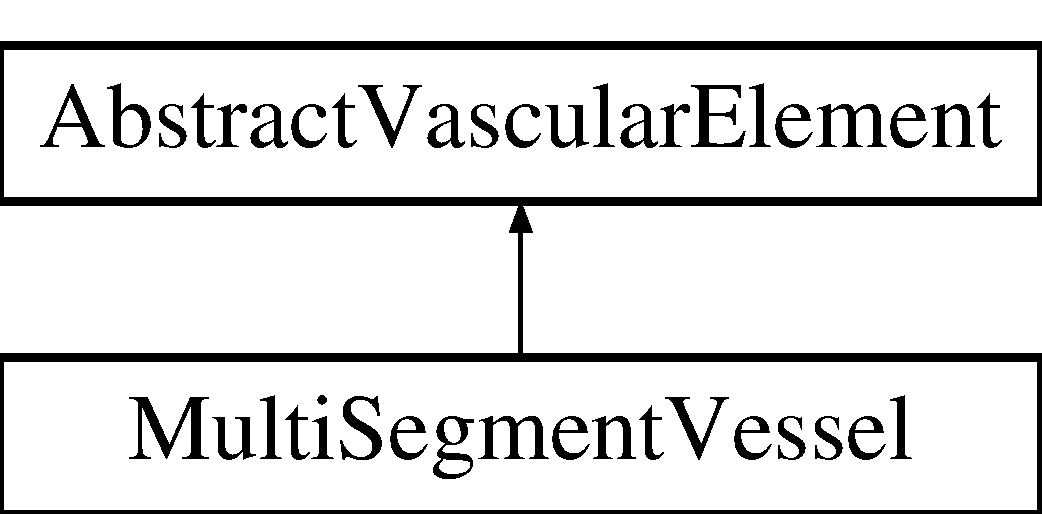
\includegraphics[height=2.000000cm]{d3/dac/class_multi_segment_vessel}
\end{center}
\end{figure}
\subsection*{Public Member Functions}
\begin{DoxyCompactItemize}
\item 
\hyperlink{class_multi_segment_vessel_aaebf85494977935ae1e0c48caf89b798}{Multi\+Segment\+Vessel} (vector$<$ \hyperlink{class_single_vessel}{Single\+Vessel} $\ast$ $>$ inner\+Segments)
\item 
\hyperlink{class_abstract_vascular_element}{Abstract\+Vascular\+Element} $\ast$ \hyperlink{class_multi_segment_vessel_acd12912a043c6c28ede419ab2f65d77f}{get\+Parent} ()
\item 
\hyperlink{class_single_vessel}{Single\+Vessel} $\ast$ \hyperlink{class_multi_segment_vessel_a3c2b7f69de853adfb6434c4e5566bea6}{get\+Parent\+Vessel\+To} (\hyperlink{structpoint}{point} xp)
\item 
vector$<$ \hyperlink{class_abstract_vascular_element}{Abstract\+Vascular\+Element} $\ast$ $>$ \& \hyperlink{class_multi_segment_vessel_a1822f40db542ad537c16499ca47ae09d}{get\+Children} ()
\item 
vector$<$ \hyperlink{class_single_vessel}{Single\+Vessel} $\ast$ $>$ $\ast$ \hyperlink{class_multi_segment_vessel_ad3220cc4fa66f851fd18b6126b250f1e}{get\+Children\+Vessel\+To} (\hyperlink{structpoint}{point} xd)
\item 
vector$<$ \hyperlink{class_single_vessel}{Single\+Vessel} $\ast$ $>$ $\ast$ \hyperlink{class_multi_segment_vessel_a7bf7eb14c3dbacf7e6fe6f9f00537d11}{get\+Vessels\+Connected\+To} (\hyperlink{structpoint}{point} p)
\item 
long long int \hyperlink{class_multi_segment_vessel_a5772718a4790089807df7b0f46f44c33}{get\+Terminals} ()
\item 
double \hyperlink{class_multi_segment_vessel_a1fdd2d4ed3fdd4e8cc62d4db6c390a27}{get\+Volume} ()
\item 
void \hyperlink{class_multi_segment_vessel_acd4b8dde6418dda9eaf3748e6ccbd0f1}{update\+Pressure} ()
\item 
double \hyperlink{class_multi_segment_vessel_ad0decc5c09f2ef4e58db122b4c511a65}{get\+Distal\+Radius} ()
\item 
double \hyperlink{class_multi_segment_vessel_a8617911dd4618bc9d75a27c894f8b66d}{get\+Proximal\+Pressure} ()
\item 
void \hyperlink{class_multi_segment_vessel_a870497c0529f2af9722f1a4a3d9d874d}{save\+Vessel\+Data} (ofstream $\ast$tree\+File)
\item 
void \hyperlink{class_multi_segment_vessel_abf6e7a21a7b57f770723050515f1bd00}{save\+Vessel\+Connectivity} (ofstream $\ast$tree\+File)
\end{DoxyCompactItemize}
\subsection*{Public Attributes}
\begin{DoxyCompactItemize}
\item 
\hyperlink{class_abstract_vascular_element_a2f7b3a097b944cd0b056fee00b93c860}{B\+R\+A\+N\+C\+H\+I\+N\+G\+\_\+\+M\+O\+DE} \hyperlink{class_multi_segment_vessel_a238ef13a0d4d9f9fb6e4bf2979386cb9}{branching\+Mode}
\item 
double \hyperlink{class_multi_segment_vessel_a512959b16b5fd0e2122a920eafe7cf0f}{length}
\item 
double \hyperlink{class_multi_segment_vessel_a31fbf5ebdd353727814fc4ec83600e6a}{local\+Resistance}
\item 
double \hyperlink{class_multi_segment_vessel_af4b7aed9f6b921d4b33ceea99c813952}{tree\+Volume}
\end{DoxyCompactItemize}
\subsection*{Additional Inherited Members}


\subsection{Detailed Description}
Vessel composed by a set of \hyperlink{class_single_vessel}{Single\+Vessel} structures in serie with only bifurcations at its ends. 

\subsection{Constructor \& Destructor Documentation}
\index{Multi\+Segment\+Vessel@{Multi\+Segment\+Vessel}!Multi\+Segment\+Vessel@{Multi\+Segment\+Vessel}}
\index{Multi\+Segment\+Vessel@{Multi\+Segment\+Vessel}!Multi\+Segment\+Vessel@{Multi\+Segment\+Vessel}}
\subsubsection[{\texorpdfstring{Multi\+Segment\+Vessel(vector$<$ Single\+Vessel $\ast$ $>$ inner\+Segments)}{MultiSegmentVessel(vector< SingleVessel * > innerSegments)}}]{\setlength{\rightskip}{0pt plus 5cm}Multi\+Segment\+Vessel\+::\+Multi\+Segment\+Vessel (
\begin{DoxyParamCaption}
\item[{vector$<$ {\bf Single\+Vessel} $\ast$ $>$}]{inner\+Segments}
\end{DoxyParamCaption}
)}\hypertarget{class_multi_segment_vessel_aaebf85494977935ae1e0c48caf89b798}{}\label{class_multi_segment_vessel_aaebf85494977935ae1e0c48caf89b798}
Creates a \hyperlink{class_multi_segment_vessel}{Multi\+Segment\+Vessel} from a vector of contiguous vessels ordered from proximal to distal position. 
\begin{DoxyParams}{Parameters}
{\em inner\+Segments} & \\
\hline
\end{DoxyParams}


\subsection{Member Function Documentation}
\index{Multi\+Segment\+Vessel@{Multi\+Segment\+Vessel}!get\+Children@{get\+Children}}
\index{get\+Children@{get\+Children}!Multi\+Segment\+Vessel@{Multi\+Segment\+Vessel}}
\subsubsection[{\texorpdfstring{get\+Children()}{getChildren()}}]{\setlength{\rightskip}{0pt plus 5cm}vector$<$ {\bf Abstract\+Vascular\+Element} $\ast$ $>$ \& Multi\+Segment\+Vessel\+::get\+Children (
\begin{DoxyParamCaption}
{}
\end{DoxyParamCaption}
)\hspace{0.3cm}{\ttfamily [virtual]}}\hypertarget{class_multi_segment_vessel_a1822f40db542ad537c16499ca47ae09d}{}\label{class_multi_segment_vessel_a1822f40db542ad537c16499ca47ae09d}
Returns all the children vessels to this vascular element. \begin{DoxyReturn}{Returns}
Children vessels to this vascular element. 
\end{DoxyReturn}


Implements \hyperlink{class_abstract_vascular_element_ae9cf2675f971fa470c74403c8b923f7d}{Abstract\+Vascular\+Element}.

\index{Multi\+Segment\+Vessel@{Multi\+Segment\+Vessel}!get\+Children\+Vessel\+To@{get\+Children\+Vessel\+To}}
\index{get\+Children\+Vessel\+To@{get\+Children\+Vessel\+To}!Multi\+Segment\+Vessel@{Multi\+Segment\+Vessel}}
\subsubsection[{\texorpdfstring{get\+Children\+Vessel\+To(point xd)}{getChildrenVesselTo(point xd)}}]{\setlength{\rightskip}{0pt plus 5cm}vector$<$ {\bf Single\+Vessel} $\ast$ $>$ $\ast$ Multi\+Segment\+Vessel\+::get\+Children\+Vessel\+To (
\begin{DoxyParamCaption}
\item[{{\bf point}}]{xd}
\end{DoxyParamCaption}
)\hspace{0.3cm}{\ttfamily [virtual]}}\hypertarget{class_multi_segment_vessel_ad3220cc4fa66f851fd18b6126b250f1e}{}\label{class_multi_segment_vessel_ad3220cc4fa66f851fd18b6126b250f1e}
Returns all \hyperlink{class_single_vessel}{Single\+Vessel} that are children of this vascular element. 
\begin{DoxyParams}{Parameters}
{\em xd} & Point of children vessels attachment. \\
\hline
\end{DoxyParams}
\begin{DoxyReturn}{Returns}
\hyperlink{class_single_vessel}{Single\+Vessel} that is parent for this vascular element. 
\end{DoxyReturn}


Implements \hyperlink{class_abstract_vascular_element_aac4f9650c704d920903c49270b18f717}{Abstract\+Vascular\+Element}.

\index{Multi\+Segment\+Vessel@{Multi\+Segment\+Vessel}!get\+Distal\+Radius@{get\+Distal\+Radius}}
\index{get\+Distal\+Radius@{get\+Distal\+Radius}!Multi\+Segment\+Vessel@{Multi\+Segment\+Vessel}}
\subsubsection[{\texorpdfstring{get\+Distal\+Radius()}{getDistalRadius()}}]{\setlength{\rightskip}{0pt plus 5cm}double Multi\+Segment\+Vessel\+::get\+Distal\+Radius (
\begin{DoxyParamCaption}
{}
\end{DoxyParamCaption}
)\hspace{0.3cm}{\ttfamily [virtual]}}\hypertarget{class_multi_segment_vessel_ad0decc5c09f2ef4e58db122b4c511a65}{}\label{class_multi_segment_vessel_ad0decc5c09f2ef4e58db122b4c511a65}
Returns the radius at the distal point of the vessel. \begin{DoxyReturn}{Returns}
Radius at the distal point of the vessel. 
\end{DoxyReturn}


Implements \hyperlink{class_abstract_vascular_element_a3880bed8d0a9223107bcee195bb89e51}{Abstract\+Vascular\+Element}.

\index{Multi\+Segment\+Vessel@{Multi\+Segment\+Vessel}!get\+Parent@{get\+Parent}}
\index{get\+Parent@{get\+Parent}!Multi\+Segment\+Vessel@{Multi\+Segment\+Vessel}}
\subsubsection[{\texorpdfstring{get\+Parent()}{getParent()}}]{\setlength{\rightskip}{0pt plus 5cm}{\bf Abstract\+Vascular\+Element} $\ast$ Multi\+Segment\+Vessel\+::get\+Parent (
\begin{DoxyParamCaption}
{}
\end{DoxyParamCaption}
)\hspace{0.3cm}{\ttfamily [virtual]}}\hypertarget{class_multi_segment_vessel_acd12912a043c6c28ede419ab2f65d77f}{}\label{class_multi_segment_vessel_acd12912a043c6c28ede419ab2f65d77f}
Returns its parental \hyperlink{class_abstract_vascular_element}{Abstract\+Vascular\+Element}. \begin{DoxyReturn}{Returns}
\hyperlink{class_abstract_vascular_element}{Abstract\+Vascular\+Element} proximally attached. 
\end{DoxyReturn}


Implements \hyperlink{class_abstract_vascular_element_aab59dfe7c6d4c846cb8f341727be8261}{Abstract\+Vascular\+Element}.

\index{Multi\+Segment\+Vessel@{Multi\+Segment\+Vessel}!get\+Parent\+Vessel\+To@{get\+Parent\+Vessel\+To}}
\index{get\+Parent\+Vessel\+To@{get\+Parent\+Vessel\+To}!Multi\+Segment\+Vessel@{Multi\+Segment\+Vessel}}
\subsubsection[{\texorpdfstring{get\+Parent\+Vessel\+To(point xp)}{getParentVesselTo(point xp)}}]{\setlength{\rightskip}{0pt plus 5cm}{\bf Single\+Vessel} $\ast$ Multi\+Segment\+Vessel\+::get\+Parent\+Vessel\+To (
\begin{DoxyParamCaption}
\item[{{\bf point}}]{xp}
\end{DoxyParamCaption}
)\hspace{0.3cm}{\ttfamily [virtual]}}\hypertarget{class_multi_segment_vessel_a3c2b7f69de853adfb6434c4e5566bea6}{}\label{class_multi_segment_vessel_a3c2b7f69de853adfb6434c4e5566bea6}
Returns the \hyperlink{class_single_vessel}{Single\+Vessel} that is parent for this vascular element. 
\begin{DoxyParams}{Parameters}
{\em xp} & Point of parent vessel attachment. \\
\hline
\end{DoxyParams}
\begin{DoxyReturn}{Returns}
\hyperlink{class_single_vessel}{Single\+Vessel} that is parent for this vascular element. 
\end{DoxyReturn}


Implements \hyperlink{class_abstract_vascular_element_a4007ab14544d8fb5cacf5c610e9b0e5d}{Abstract\+Vascular\+Element}.

\index{Multi\+Segment\+Vessel@{Multi\+Segment\+Vessel}!get\+Proximal\+Pressure@{get\+Proximal\+Pressure}}
\index{get\+Proximal\+Pressure@{get\+Proximal\+Pressure}!Multi\+Segment\+Vessel@{Multi\+Segment\+Vessel}}
\subsubsection[{\texorpdfstring{get\+Proximal\+Pressure()}{getProximalPressure()}}]{\setlength{\rightskip}{0pt plus 5cm}double Multi\+Segment\+Vessel\+::get\+Proximal\+Pressure (
\begin{DoxyParamCaption}
{}
\end{DoxyParamCaption}
)\hspace{0.3cm}{\ttfamily [virtual]}}\hypertarget{class_multi_segment_vessel_a8617911dd4618bc9d75a27c894f8b66d}{}\label{class_multi_segment_vessel_a8617911dd4618bc9d75a27c894f8b66d}
Returns the pressure at the proximal point of the vessel. \begin{DoxyReturn}{Returns}
Pressure at the proximal point of the vessel. 
\end{DoxyReturn}


Implements \hyperlink{class_abstract_vascular_element_aa486370af563a9ea9bfcdcde8ee38426}{Abstract\+Vascular\+Element}.

\index{Multi\+Segment\+Vessel@{Multi\+Segment\+Vessel}!get\+Terminals@{get\+Terminals}}
\index{get\+Terminals@{get\+Terminals}!Multi\+Segment\+Vessel@{Multi\+Segment\+Vessel}}
\subsubsection[{\texorpdfstring{get\+Terminals()}{getTerminals()}}]{\setlength{\rightskip}{0pt plus 5cm}long long int Multi\+Segment\+Vessel\+::get\+Terminals (
\begin{DoxyParamCaption}
{}
\end{DoxyParamCaption}
)\hspace{0.3cm}{\ttfamily [virtual]}}\hypertarget{class_multi_segment_vessel_a5772718a4790089807df7b0f46f44c33}{}\label{class_multi_segment_vessel_a5772718a4790089807df7b0f46f44c33}
Returns all the inner terminals in the current vascular element. \begin{DoxyReturn}{Returns}
Terminals in the current vascular element. 
\end{DoxyReturn}


Implements \hyperlink{class_abstract_vascular_element_a85d8d19d6f92a4e7cc95cc0f8f5a59c9}{Abstract\+Vascular\+Element}.

\index{Multi\+Segment\+Vessel@{Multi\+Segment\+Vessel}!get\+Vessels\+Connected\+To@{get\+Vessels\+Connected\+To}}
\index{get\+Vessels\+Connected\+To@{get\+Vessels\+Connected\+To}!Multi\+Segment\+Vessel@{Multi\+Segment\+Vessel}}
\subsubsection[{\texorpdfstring{get\+Vessels\+Connected\+To(point p)}{getVesselsConnectedTo(point p)}}]{\setlength{\rightskip}{0pt plus 5cm}vector$<$ {\bf Single\+Vessel} $\ast$ $>$ $\ast$ Multi\+Segment\+Vessel\+::get\+Vessels\+Connected\+To (
\begin{DoxyParamCaption}
\item[{{\bf point}}]{p}
\end{DoxyParamCaption}
)\hspace{0.3cm}{\ttfamily [virtual]}}\hypertarget{class_multi_segment_vessel_a7bf7eb14c3dbacf7e6fe6f9f00537d11}{}\label{class_multi_segment_vessel_a7bf7eb14c3dbacf7e6fe6f9f00537d11}
Returns all vessels in this vascular structure connected to point {\ttfamily p}. 
\begin{DoxyParams}{Parameters}
{\em p} & Point at which all target vessels are connected to. \\
\hline
\end{DoxyParams}
\begin{DoxyReturn}{Returns}
Set of vessels connected to {\ttfamily p}. 
\end{DoxyReturn}


Implements \hyperlink{class_abstract_vascular_element_a7720067153a223d373c26e14155553e3}{Abstract\+Vascular\+Element}.

\index{Multi\+Segment\+Vessel@{Multi\+Segment\+Vessel}!get\+Volume@{get\+Volume}}
\index{get\+Volume@{get\+Volume}!Multi\+Segment\+Vessel@{Multi\+Segment\+Vessel}}
\subsubsection[{\texorpdfstring{get\+Volume()}{getVolume()}}]{\setlength{\rightskip}{0pt plus 5cm}double Multi\+Segment\+Vessel\+::get\+Volume (
\begin{DoxyParamCaption}
{}
\end{DoxyParamCaption}
)\hspace{0.3cm}{\ttfamily [virtual]}}\hypertarget{class_multi_segment_vessel_a1fdd2d4ed3fdd4e8cc62d4db6c390a27}{}\label{class_multi_segment_vessel_a1fdd2d4ed3fdd4e8cc62d4db6c390a27}
Returns the functional cost contribution of this vascular element. If any constraint --e.\+g. geometric constrains-- are violated the function must return I\+N\+F\+I\+N\+I\+TY. \begin{DoxyReturn}{Returns}
Functional cost contribution. 
\end{DoxyReturn}


Implements \hyperlink{class_abstract_vascular_element_ae4ecb632a94e89ac21f6523637bdb9cd}{Abstract\+Vascular\+Element}.

\index{Multi\+Segment\+Vessel@{Multi\+Segment\+Vessel}!save\+Vessel\+Connectivity@{save\+Vessel\+Connectivity}}
\index{save\+Vessel\+Connectivity@{save\+Vessel\+Connectivity}!Multi\+Segment\+Vessel@{Multi\+Segment\+Vessel}}
\subsubsection[{\texorpdfstring{save\+Vessel\+Connectivity(ofstream $\ast$tree\+File)}{saveVesselConnectivity(ofstream *treeFile)}}]{\setlength{\rightskip}{0pt plus 5cm}void Multi\+Segment\+Vessel\+::save\+Vessel\+Connectivity (
\begin{DoxyParamCaption}
\item[{ofstream $\ast$}]{tree\+File}
\end{DoxyParamCaption}
)\hspace{0.3cm}{\ttfamily [virtual]}}\hypertarget{class_multi_segment_vessel_abf6e7a21a7b57f770723050515f1bd00}{}\label{class_multi_segment_vessel_abf6e7a21a7b57f770723050515f1bd00}
Writes connectivity of this vessel at the file associated to {\ttfamily tree\+File} stream. 
\begin{DoxyParams}{Parameters}
{\em tree\+File} & Output file stream. \\
\hline
\end{DoxyParams}


Implements \hyperlink{class_abstract_vascular_element_a878c2826beb1a549c28659182760fbab}{Abstract\+Vascular\+Element}.

\index{Multi\+Segment\+Vessel@{Multi\+Segment\+Vessel}!save\+Vessel\+Data@{save\+Vessel\+Data}}
\index{save\+Vessel\+Data@{save\+Vessel\+Data}!Multi\+Segment\+Vessel@{Multi\+Segment\+Vessel}}
\subsubsection[{\texorpdfstring{save\+Vessel\+Data(ofstream $\ast$tree\+File)}{saveVesselData(ofstream *treeFile)}}]{\setlength{\rightskip}{0pt plus 5cm}void Multi\+Segment\+Vessel\+::save\+Vessel\+Data (
\begin{DoxyParamCaption}
\item[{ofstream $\ast$}]{tree\+File}
\end{DoxyParamCaption}
)\hspace{0.3cm}{\ttfamily [virtual]}}\hypertarget{class_multi_segment_vessel_a870497c0529f2af9722f1a4a3d9d874d}{}\label{class_multi_segment_vessel_a870497c0529f2af9722f1a4a3d9d874d}
Writes the vessel data at the file associated to {\ttfamily tree\+File} stream. 
\begin{DoxyParams}{Parameters}
{\em tree\+File} & Output file stream. \\
\hline
\end{DoxyParams}


Implements \hyperlink{class_abstract_vascular_element_aff5f129b31f0c82aebf2d7387859914d}{Abstract\+Vascular\+Element}.

\index{Multi\+Segment\+Vessel@{Multi\+Segment\+Vessel}!update\+Pressure@{update\+Pressure}}
\index{update\+Pressure@{update\+Pressure}!Multi\+Segment\+Vessel@{Multi\+Segment\+Vessel}}
\subsubsection[{\texorpdfstring{update\+Pressure()}{updatePressure()}}]{\setlength{\rightskip}{0pt plus 5cm}void Multi\+Segment\+Vessel\+::update\+Pressure (
\begin{DoxyParamCaption}
{}
\end{DoxyParamCaption}
)\hspace{0.3cm}{\ttfamily [virtual]}}\hypertarget{class_multi_segment_vessel_acd4b8dde6418dda9eaf3748e6ccbd0f1}{}\label{class_multi_segment_vessel_acd4b8dde6418dda9eaf3748e6ccbd0f1}
Updates vascular element pressure from children to parent direction. 

Implements \hyperlink{class_abstract_vascular_element_a258a830359614d0217e820293a9bdaa9}{Abstract\+Vascular\+Element}.



\subsection{Member Data Documentation}
\index{Multi\+Segment\+Vessel@{Multi\+Segment\+Vessel}!branching\+Mode@{branching\+Mode}}
\index{branching\+Mode@{branching\+Mode}!Multi\+Segment\+Vessel@{Multi\+Segment\+Vessel}}
\subsubsection[{\texorpdfstring{branching\+Mode}{branchingMode}}]{\setlength{\rightskip}{0pt plus 5cm}{\bf B\+R\+A\+N\+C\+H\+I\+N\+G\+\_\+\+M\+O\+DE} Multi\+Segment\+Vessel\+::branching\+Mode}\hypertarget{class_multi_segment_vessel_a238ef13a0d4d9f9fb6e4bf2979386cb9}{}\label{class_multi_segment_vessel_a238ef13a0d4d9f9fb6e4bf2979386cb9}
Indicates the hotspots where the vessel can bifurcate. \index{Multi\+Segment\+Vessel@{Multi\+Segment\+Vessel}!length@{length}}
\index{length@{length}!Multi\+Segment\+Vessel@{Multi\+Segment\+Vessel}}
\subsubsection[{\texorpdfstring{length}{length}}]{\setlength{\rightskip}{0pt plus 5cm}double Multi\+Segment\+Vessel\+::length}\hypertarget{class_multi_segment_vessel_a512959b16b5fd0e2122a920eafe7cf0f}{}\label{class_multi_segment_vessel_a512959b16b5fd0e2122a920eafe7cf0f}
Distance between x\+Prox and x\+Dist. \index{Multi\+Segment\+Vessel@{Multi\+Segment\+Vessel}!local\+Resistance@{local\+Resistance}}
\index{local\+Resistance@{local\+Resistance}!Multi\+Segment\+Vessel@{Multi\+Segment\+Vessel}}
\subsubsection[{\texorpdfstring{local\+Resistance}{localResistance}}]{\setlength{\rightskip}{0pt plus 5cm}double Multi\+Segment\+Vessel\+::local\+Resistance}\hypertarget{class_multi_segment_vessel_a31fbf5ebdd353727814fc4ec83600e6a}{}\label{class_multi_segment_vessel_a31fbf5ebdd353727814fc4ec83600e6a}
Reduced fluid-\/dynamic resistance. \index{Multi\+Segment\+Vessel@{Multi\+Segment\+Vessel}!tree\+Volume@{tree\+Volume}}
\index{tree\+Volume@{tree\+Volume}!Multi\+Segment\+Vessel@{Multi\+Segment\+Vessel}}
\subsubsection[{\texorpdfstring{tree\+Volume}{treeVolume}}]{\setlength{\rightskip}{0pt plus 5cm}double Multi\+Segment\+Vessel\+::tree\+Volume}\hypertarget{class_multi_segment_vessel_af4b7aed9f6b921d4b33ceea99c813952}{}\label{class_multi_segment_vessel_af4b7aed9f6b921d4b33ceea99c813952}
Volume of this down tree branch. 

The documentation for this class was generated from the following files\+:\begin{DoxyCompactItemize}
\item 
structures/vascular\+Elements/Multi\+Segment\+Vessel.\+h\item 
structures/vascular\+Elements/Multi\+Segment\+Vessel.\+cpp\end{DoxyCompactItemize}

\hypertarget{class_normal_distribution_generator}{}\section{Normal\+Distribution\+Generator Class Reference}
\label{class_normal_distribution_generator}\index{Normal\+Distribution\+Generator@{Normal\+Distribution\+Generator}}
Inheritance diagram for Normal\+Distribution\+Generator\+:\begin{figure}[H]
\begin{center}
\leavevmode
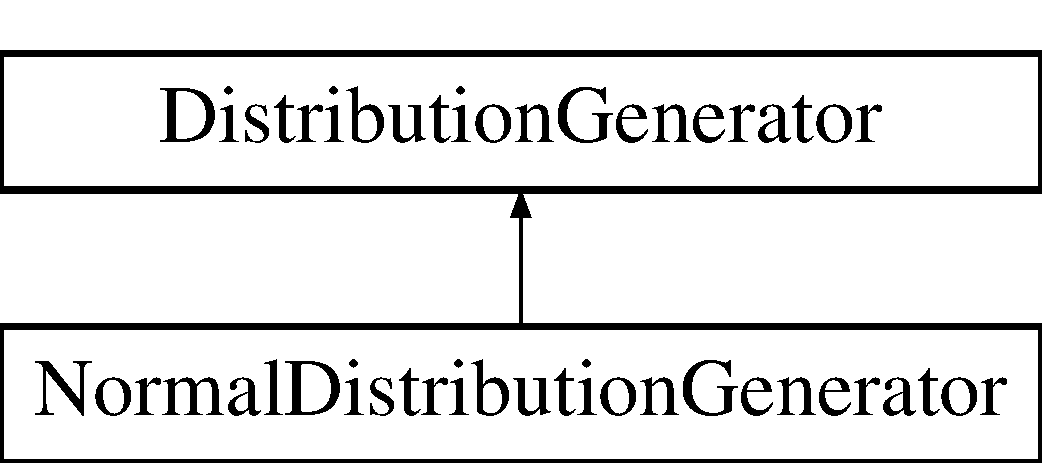
\includegraphics[height=2.000000cm]{df/d2c/class_normal_distribution_generator}
\end{center}
\end{figure}
\subsection*{Additional Inherited Members}


The documentation for this class was generated from the following files\+:\begin{DoxyCompactItemize}
\item 
structures/domain/Normal\+Distribution\+Generator.\+h\item 
structures/domain/Normal\+Distribution\+Generator.\+cpp\end{DoxyCompactItemize}

\hypertarget{class_parallelepiped_creator}{}\section{Parallelepiped\+Creator Class Reference}
\label{class_parallelepiped_creator}\index{Parallelepiped\+Creator@{Parallelepiped\+Creator}}


{\ttfamily \#include $<$Parallelepiped\+Creator.\+h$>$}

Inheritance diagram for Parallelepiped\+Creator\+:\begin{figure}[H]
\begin{center}
\leavevmode
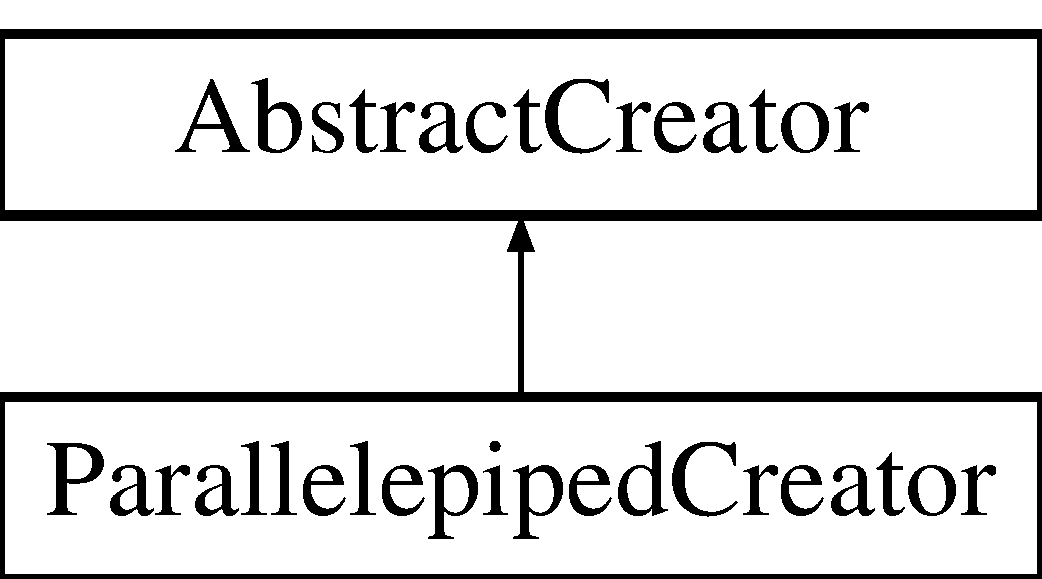
\includegraphics[height=2.000000cm]{dd/def/class_parallelepiped_creator}
\end{center}
\end{figure}
\subsection*{Public Member Functions}
\begin{DoxyCompactItemize}
\item 
\hyperlink{class_parallelepiped_creator_a90c756a533fe6590d1ea2cd236c4762f}{Parallelepiped\+Creator} (double $\ast$\hyperlink{class_parallelepiped_creator_afbbe8ed8aca059a07b2198e4e6ced522}{lb}, double $\ast$\hyperlink{class_parallelepiped_creator_a2120f519681200f2b431439b2e022e1b}{ub})
\item 
virtual \hyperlink{class_parallelepiped_creator_a1e41ac467a6423c499401dd2e7663be7}{$\sim$\+Parallelepiped\+Creator} ()
\item 
void \hyperlink{class_parallelepiped_creator_a12a54b7a1d66ac413c30327751d8ad47}{create} (string filename)
\end{DoxyCompactItemize}
\subsection*{Private Attributes}
\begin{DoxyCompactItemize}
\item 
double $\ast$ \hyperlink{class_parallelepiped_creator_afbbe8ed8aca059a07b2198e4e6ced522}{lb}
\item 
double $\ast$ \hyperlink{class_parallelepiped_creator_a2120f519681200f2b431439b2e022e1b}{ub}
\end{DoxyCompactItemize}


\subsection{Detailed Description}
Creates a V\+TP file containing a parallelepiped. 

\subsection{Constructor \& Destructor Documentation}
\index{Parallelepiped\+Creator@{Parallelepiped\+Creator}!Parallelepiped\+Creator@{Parallelepiped\+Creator}}
\index{Parallelepiped\+Creator@{Parallelepiped\+Creator}!Parallelepiped\+Creator@{Parallelepiped\+Creator}}
\subsubsection[{\texorpdfstring{Parallelepiped\+Creator(double $\ast$lb, double $\ast$ub)}{ParallelepipedCreator(double *lb, double *ub)}}]{\setlength{\rightskip}{0pt plus 5cm}Parallelepiped\+Creator\+::\+Parallelepiped\+Creator (
\begin{DoxyParamCaption}
\item[{double $\ast$}]{lb, }
\item[{double $\ast$}]{ub}
\end{DoxyParamCaption}
)}\hypertarget{class_parallelepiped_creator_a90c756a533fe6590d1ea2cd236c4762f}{}\label{class_parallelepiped_creator_a90c756a533fe6590d1ea2cd236c4762f}
Initialize the inner variables of the object. Vertexes {\ttfamily lb} and {\ttfamily ub} must be opposite vertexes of the parallelepiped. 
\begin{DoxyParams}{Parameters}
{\em lb} & Vertex v1. \\
\hline
{\em ub} & Vertex v2. \\
\hline
\end{DoxyParams}
\index{Parallelepiped\+Creator@{Parallelepiped\+Creator}!````~Parallelepiped\+Creator@{$\sim$\+Parallelepiped\+Creator}}
\index{````~Parallelepiped\+Creator@{$\sim$\+Parallelepiped\+Creator}!Parallelepiped\+Creator@{Parallelepiped\+Creator}}
\subsubsection[{\texorpdfstring{$\sim$\+Parallelepiped\+Creator()}{~ParallelepipedCreator()}}]{\setlength{\rightskip}{0pt plus 5cm}Parallelepiped\+Creator\+::$\sim$\+Parallelepiped\+Creator (
\begin{DoxyParamCaption}
{}
\end{DoxyParamCaption}
)\hspace{0.3cm}{\ttfamily [virtual]}}\hypertarget{class_parallelepiped_creator_a1e41ac467a6423c499401dd2e7663be7}{}\label{class_parallelepiped_creator_a1e41ac467a6423c499401dd2e7663be7}
Standard destructor. 

\subsection{Member Function Documentation}
\index{Parallelepiped\+Creator@{Parallelepiped\+Creator}!create@{create}}
\index{create@{create}!Parallelepiped\+Creator@{Parallelepiped\+Creator}}
\subsubsection[{\texorpdfstring{create(string filename)}{create(string filename)}}]{\setlength{\rightskip}{0pt plus 5cm}void Parallelepiped\+Creator\+::create (
\begin{DoxyParamCaption}
\item[{string}]{filename}
\end{DoxyParamCaption}
)\hspace{0.3cm}{\ttfamily [virtual]}}\hypertarget{class_parallelepiped_creator_a12a54b7a1d66ac413c30327751d8ad47}{}\label{class_parallelepiped_creator_a12a54b7a1d66ac413c30327751d8ad47}
Persist the object in a file with V\+TP format. 
\begin{DoxyParams}{Parameters}
{\em filename} & Save file for the current object. \\
\hline
\end{DoxyParams}


Implements \hyperlink{class_abstract_creator_a1991e446444ffea2b85216b64f2dcf9e}{Abstract\+Creator}.



\subsection{Member Data Documentation}
\index{Parallelepiped\+Creator@{Parallelepiped\+Creator}!lb@{lb}}
\index{lb@{lb}!Parallelepiped\+Creator@{Parallelepiped\+Creator}}
\subsubsection[{\texorpdfstring{lb}{lb}}]{\setlength{\rightskip}{0pt plus 5cm}double$\ast$ Parallelepiped\+Creator\+::lb\hspace{0.3cm}{\ttfamily [private]}}\hypertarget{class_parallelepiped_creator_afbbe8ed8aca059a07b2198e4e6ced522}{}\label{class_parallelepiped_creator_afbbe8ed8aca059a07b2198e4e6ced522}
Vertex 1 \index{Parallelepiped\+Creator@{Parallelepiped\+Creator}!ub@{ub}}
\index{ub@{ub}!Parallelepiped\+Creator@{Parallelepiped\+Creator}}
\subsubsection[{\texorpdfstring{ub}{ub}}]{\setlength{\rightskip}{0pt plus 5cm}double$\ast$ Parallelepiped\+Creator\+::ub\hspace{0.3cm}{\ttfamily [private]}}\hypertarget{class_parallelepiped_creator_a2120f519681200f2b431439b2e022e1b}{}\label{class_parallelepiped_creator_a2120f519681200f2b431439b2e022e1b}
Vertex 2 

The documentation for this class was generated from the following files\+:\begin{DoxyCompactItemize}
\item 
creators/Parallelepiped\+Creator.\+h\item 
creators/Parallelepiped\+Creator.\+cpp\end{DoxyCompactItemize}

\hypertarget{class_partially_vascularized_domain}{}\section{Partially\+Vascularized\+Domain Class Reference}
\label{class_partially_vascularized_domain}\index{Partially\+Vascularized\+Domain@{Partially\+Vascularized\+Domain}}


{\ttfamily \#include $<$Partially\+Vascularized\+Domain.\+h$>$}

Inheritance diagram for Partially\+Vascularized\+Domain\+:\begin{figure}[H]
\begin{center}
\leavevmode
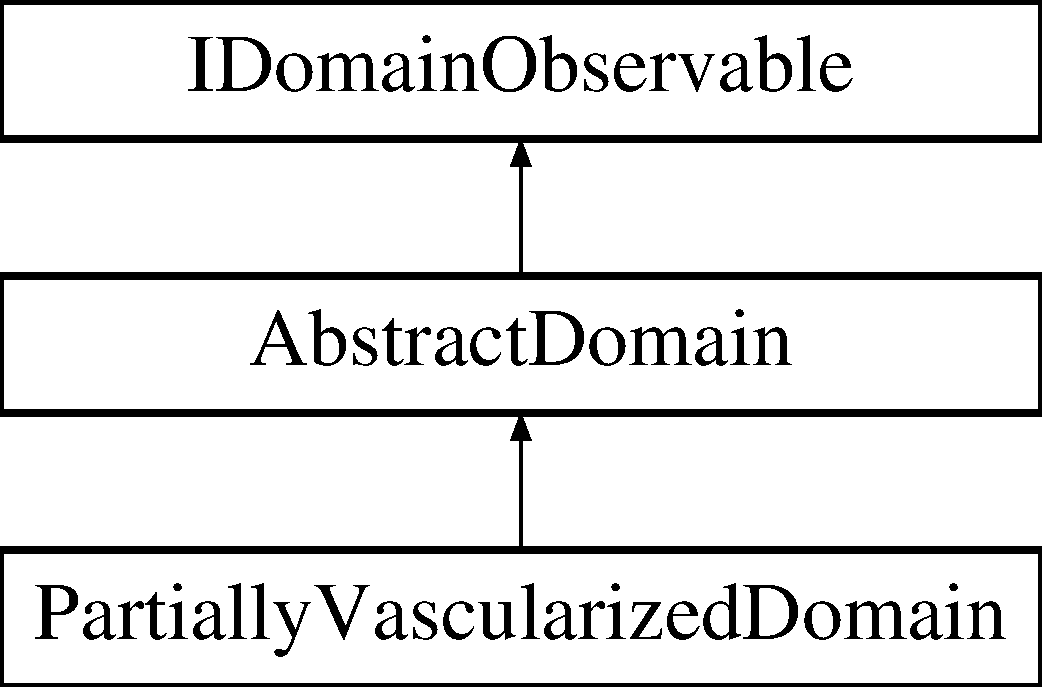
\includegraphics[height=3.000000cm]{d0/d32/class_partially_vascularized_domain}
\end{center}
\end{figure}
\subsection*{Public Member Functions}
\begin{DoxyCompactItemize}
\item 
\hyperlink{class_partially_vascularized_domain_a98e6ef8e987c36fda10852347433ac3e}{Partially\+Vascularized\+Domain} (string filename\+Hull, vector$<$ string $>$ filename\+Vascular\+Regions, vector$<$ string $>$ filename\+Non\+Vascular\+Regions, \hyperlink{class_generator_data}{Generator\+Data} $\ast$\hyperlink{class_abstract_domain_aa37fbabc2bfa92c574f7db7544016b53}{instance\+Data})
\item 
\hyperlink{class_partially_vascularized_domain_a8da1612c7f4a4599659b9683e1f6da0f}{Partially\+Vascularized\+Domain} (string filename\+Hull, vector$<$ string $>$ filename\+Vascular\+Regions, vector$<$ string $>$ filename\+Non\+Vascular\+Regions, int \hyperlink{class_partially_vascularized_domain_ae88320ec5cef5465ad2c74ce201d5131}{n\+Draw}, \hyperlink{class_generator_data}{Generator\+Data} $\ast$\hyperlink{class_abstract_domain_aa37fbabc2bfa92c574f7db7544016b53}{instance\+Data})
\item 
\hyperlink{class_partially_vascularized_domain_a430194cae85988ff828b8d5deb46e7bc}{Partially\+Vascularized\+Domain} (string filename\+Hull, vector$<$ string $>$ filename\+Vascular\+Regions, vector$<$ string $>$ filename\+Non\+Vascular\+Regions, int \hyperlink{class_partially_vascularized_domain_ae88320ec5cef5465ad2c74ce201d5131}{n\+Draw}, int \hyperlink{class_partially_vascularized_domain_a443b5b60ce756ea5bfb05c628ed4af0d}{seed}, \hyperlink{class_generator_data}{Generator\+Data} $\ast$\hyperlink{class_abstract_domain_aa37fbabc2bfa92c574f7db7544016b53}{instance\+Data})
\item 
int \hyperlink{class_partially_vascularized_domain_a485e0e573369f76ef59477fc5ac8ea9b}{is\+Segment\+Inside} (\hyperlink{structpoint}{point} xs, \hyperlink{structpoint}{point} xf)
\item 
double \hyperlink{class_partially_vascularized_domain_a1ec0827e05801a1a3219cbd4e87ac64c}{get\+Characteristic\+Length} ()
\item 
double \hyperlink{class_partially_vascularized_domain_a7cfa7a304d236b933311f8ac5149662e}{get\+D\+Lim} (long long int n\+Vessels, double factor)
\item 
double $\ast$ \hyperlink{class_partially_vascularized_domain_a379893eff3b1612932f4689a478e73ee}{get\+Local\+Neighborhood} (\hyperlink{structpoint}{point} p, long long int n\+Vessels)
\item 
double \hyperlink{class_partially_vascularized_domain_a88c04b73a8ffd9e8ddbc4a1c118a1795}{get\+Size} ()
\item 
virtual \hyperlink{structpoint}{point} \hyperlink{class_partially_vascularized_domain_a817dcd8122892b14ed112135aa4a1fe0}{get\+Random\+Point} ()
\item 
vtk\+Smart\+Pointer$<$ vtk\+O\+B\+B\+Tree $>$ \& \hyperlink{class_partially_vascularized_domain_aaa408e316948645dd383abfdd327c733}{get\+Locator} ()
\item 
int \hyperlink{class_partially_vascularized_domain_aefb222fe10e4691e965b3a2035e0b119}{get\+Draw} ()
\item 
deque$<$ \hyperlink{structpoint}{point} $>$ \& \hyperlink{class_partially_vascularized_domain_abbfb8f486b00e62117b564874a454395}{get\+Random\+Inner\+Points} ()
\item 
vtk\+Smart\+Pointer$<$ vtk\+Poly\+Data $>$ \& \hyperlink{class_partially_vascularized_domain_aa2acdedb98eb9cd168b9ab4cfa38c485}{get\+Vtk\+Geometry} ()
\end{DoxyCompactItemize}
\subsection*{Protected Member Functions}
\begin{DoxyCompactItemize}
\item 
void {\bfseries generate\+Random\+Points} ()\hypertarget{class_partially_vascularized_domain_a2cd16ecba9744376ed887ac5c384f8d6}{}\label{class_partially_vascularized_domain_a2cd16ecba9744376ed887ac5c384f8d6}

\item 
void {\bfseries remove\+Random\+Outer\+Points} ()\hypertarget{class_partially_vascularized_domain_af607ad95d6ee6f3642d53cef956c22d2}{}\label{class_partially_vascularized_domain_af607ad95d6ee6f3642d53cef956c22d2}

\end{DoxyCompactItemize}
\subsection*{Protected Attributes}
\begin{DoxyCompactItemize}
\item 
deque$<$ \hyperlink{structpoint}{point} $>$ {\bfseries random\+Inner\+Points}\hypertarget{class_partially_vascularized_domain_abe9eaae7ebdf88e4bb1f9389d697c5c3}{}\label{class_partially_vascularized_domain_abe9eaae7ebdf88e4bb1f9389d697c5c3}

\end{DoxyCompactItemize}
\subsection*{Private Attributes}
\begin{DoxyCompactItemize}
\item 
vtk\+Smart\+Pointer$<$ vtk\+Poly\+Data $>$ \hyperlink{class_partially_vascularized_domain_af4d0cd0bc35113adccb312f4b07dcd72}{vtk\+Transport\+Region}
\item 
vector$<$ vtk\+Smart\+Pointer$<$ vtk\+Poly\+Data $>$ $>$ \hyperlink{class_partially_vascularized_domain_aeacff4635f73c185d8a83a3a824b49cb}{vtk\+Vascularized\+Regions}
\item 
vector$<$ vtk\+Smart\+Pointer$<$ vtk\+Poly\+Data $>$ $>$ \hyperlink{class_partially_vascularized_domain_a725b3a41a8c28011def02f193121b99b}{vtk\+Hollow\+Regions}
\item 
vtk\+Smart\+Pointer$<$ vtk\+O\+B\+B\+Tree $>$ \hyperlink{class_partially_vascularized_domain_a3e4d13820b8ed9beea9bf9d3bfc807a2}{locator}
\item 
vector$<$ vtk\+Smart\+Pointer$<$ vtk\+O\+B\+B\+Tree $>$ $>$ \hyperlink{class_partially_vascularized_domain_abce195c2c0bd9f52cf932560539aec57}{hollow\+Locators}
\item 
double \hyperlink{class_partially_vascularized_domain_ac79741173831cc9628ccf7ad193f2812}{characteristic\+Length}
\item 
int \hyperlink{class_partially_vascularized_domain_ae88320ec5cef5465ad2c74ce201d5131}{n\+Draw}
\item 
int \hyperlink{class_partially_vascularized_domain_a443b5b60ce756ea5bfb05c628ed4af0d}{seed} = -\/1
\item 
mt19937 \hyperlink{class_partially_vascularized_domain_a78f13fd2210c58eae813d057b580c3cc}{generator}
\end{DoxyCompactItemize}


\subsection{Detailed Description}
This domain features three different type of volumes\+: (i) transport volume; (ii) vascularized volumes; (iii) non-\/vascularized volumes. A transport volume allows that existent vessels within it, create terminals to vascularized volumes. Thus, its space may prone anastomose from existent arteries to vascularized regions, but no terminals can be created in it. A vascularized volume allowed the anastomose in its existent vessels and the creation of terminals within it. Lastly, non-\/vascularized volumes do not allowed vessels to enter exit nor generate terminals. It is mandatory that vascularized regions be within the transport volume. 

\subsection{Constructor \& Destructor Documentation}
\index{Partially\+Vascularized\+Domain@{Partially\+Vascularized\+Domain}!Partially\+Vascularized\+Domain@{Partially\+Vascularized\+Domain}}
\index{Partially\+Vascularized\+Domain@{Partially\+Vascularized\+Domain}!Partially\+Vascularized\+Domain@{Partially\+Vascularized\+Domain}}
\subsubsection[{\texorpdfstring{Partially\+Vascularized\+Domain(string filename\+Hull, vector$<$ string $>$ filename\+Vascular\+Regions, vector$<$ string $>$ filename\+Non\+Vascular\+Regions, Generator\+Data $\ast$instance\+Data)}{PartiallyVascularizedDomain(string filenameHull, vector< string > filenameVascularRegions, vector< string > filenameNonVascularRegions, GeneratorData *instanceData)}}]{\setlength{\rightskip}{0pt plus 5cm}Partially\+Vascularized\+Domain\+::\+Partially\+Vascularized\+Domain (
\begin{DoxyParamCaption}
\item[{string}]{filename\+Hull, }
\item[{vector$<$ string $>$}]{filename\+Vascular\+Regions, }
\item[{vector$<$ string $>$}]{filename\+Non\+Vascular\+Regions, }
\item[{{\bf Generator\+Data} $\ast$}]{instance\+Data}
\end{DoxyParamCaption}
)}\hypertarget{class_partially_vascularized_domain_a98e6ef8e987c36fda10852347433ac3e}{}\label{class_partially_vascularized_domain_a98e6ef8e987c36fda10852347433ac3e}
Constructs a domain shaped by {\ttfamily filename\+Hull} (transport domain) with vascularized and non-\/vascularized regions contained in {\ttfamily filename\+Vascular\+Regions} and {\ttfamily filename\+Non\+Vascular\+Regions} respectively. 
\begin{DoxyParams}{Parameters}
{\em filename\+Hull} & Domain description. \\
\hline
{\em filename\+Vascular\+Regions} & Vascularized regions descriptions. \\
\hline
{\em filename\+Non\+Vascular\+Regions} & Non-\/vascularized regions descriptions. \\
\hline
\end{DoxyParams}
\index{Partially\+Vascularized\+Domain@{Partially\+Vascularized\+Domain}!Partially\+Vascularized\+Domain@{Partially\+Vascularized\+Domain}}
\index{Partially\+Vascularized\+Domain@{Partially\+Vascularized\+Domain}!Partially\+Vascularized\+Domain@{Partially\+Vascularized\+Domain}}
\subsubsection[{\texorpdfstring{Partially\+Vascularized\+Domain(string filename\+Hull, vector$<$ string $>$ filename\+Vascular\+Regions, vector$<$ string $>$ filename\+Non\+Vascular\+Regions, int n\+Draw, Generator\+Data $\ast$instance\+Data)}{PartiallyVascularizedDomain(string filenameHull, vector< string > filenameVascularRegions, vector< string > filenameNonVascularRegions, int nDraw, GeneratorData *instanceData)}}]{\setlength{\rightskip}{0pt plus 5cm}Partially\+Vascularized\+Domain\+::\+Partially\+Vascularized\+Domain (
\begin{DoxyParamCaption}
\item[{string}]{filename\+Hull, }
\item[{vector$<$ string $>$}]{filename\+Vascular\+Regions, }
\item[{vector$<$ string $>$}]{filename\+Non\+Vascular\+Regions, }
\item[{int}]{n\+Draw, }
\item[{{\bf Generator\+Data} $\ast$}]{instance\+Data}
\end{DoxyParamCaption}
)}\hypertarget{class_partially_vascularized_domain_a8da1612c7f4a4599659b9683e1f6da0f}{}\label{class_partially_vascularized_domain_a8da1612c7f4a4599659b9683e1f6da0f}
Constructs a domain shaped by {\ttfamily filename\+Hull} (transport domain) with vascularized and non-\/vascularized regions contained in {\ttfamily filename\+Vascular\+Regions} and {\ttfamily filename\+Non\+Vascular\+Regions} respectively. Also, itgenerates batches of {\ttfamily n\+Draw} random points each time that the domain is with no more points. 
\begin{DoxyParams}{Parameters}
{\em filename\+Hull} & Domain description. \\
\hline
{\em filename\+Vascular\+Regions} & Vascularized regions descriptions. \\
\hline
{\em filename\+Non\+Vascular\+Regions} & Non-\/vascularized regions descriptions. \\
\hline
{\em n\+Draw} & Random points generated at each batch. \\
\hline
\end{DoxyParams}
\index{Partially\+Vascularized\+Domain@{Partially\+Vascularized\+Domain}!Partially\+Vascularized\+Domain@{Partially\+Vascularized\+Domain}}
\index{Partially\+Vascularized\+Domain@{Partially\+Vascularized\+Domain}!Partially\+Vascularized\+Domain@{Partially\+Vascularized\+Domain}}
\subsubsection[{\texorpdfstring{Partially\+Vascularized\+Domain(string filename\+Hull, vector$<$ string $>$ filename\+Vascular\+Regions, vector$<$ string $>$ filename\+Non\+Vascular\+Regions, int n\+Draw, int seed, Generator\+Data $\ast$instance\+Data)}{PartiallyVascularizedDomain(string filenameHull, vector< string > filenameVascularRegions, vector< string > filenameNonVascularRegions, int nDraw, int seed, GeneratorData *instanceData)}}]{\setlength{\rightskip}{0pt plus 5cm}Partially\+Vascularized\+Domain\+::\+Partially\+Vascularized\+Domain (
\begin{DoxyParamCaption}
\item[{string}]{filename\+Hull, }
\item[{vector$<$ string $>$}]{filename\+Vascular\+Regions, }
\item[{vector$<$ string $>$}]{filename\+Non\+Vascular\+Regions, }
\item[{int}]{n\+Draw, }
\item[{int}]{seed, }
\item[{{\bf Generator\+Data} $\ast$}]{instance\+Data}
\end{DoxyParamCaption}
)}\hypertarget{class_partially_vascularized_domain_a430194cae85988ff828b8d5deb46e7bc}{}\label{class_partially_vascularized_domain_a430194cae85988ff828b8d5deb46e7bc}
Constructs a domain shaped by {\ttfamily filename\+Hull} (transport domain) with vascularized and non-\/vascularized regions contained in {\ttfamily filename\+Vascular\+Regions} and {\ttfamily filename\+Non\+Vascular\+Regions} respectively. Also, itgenerates batches of {\ttfamily n\+Draw} random points each time that the domain is with no more points. 
\begin{DoxyParams}{Parameters}
{\em filename\+Hull} & Domain description. \\
\hline
{\em filename\+Vascular\+Regions} & Vascularized regions descriptions. \\
\hline
{\em filename\+Non\+Vascular\+Regions} & Non-\/vascularized regions descriptions. \\
\hline
{\em n\+Draw} & Random points generated at each batch. \\
\hline
{\em seed} & Seed for random points generation. \\
\hline
\end{DoxyParams}


\subsection{Member Function Documentation}
\index{Partially\+Vascularized\+Domain@{Partially\+Vascularized\+Domain}!get\+Characteristic\+Length@{get\+Characteristic\+Length}}
\index{get\+Characteristic\+Length@{get\+Characteristic\+Length}!Partially\+Vascularized\+Domain@{Partially\+Vascularized\+Domain}}
\subsubsection[{\texorpdfstring{get\+Characteristic\+Length()}{getCharacteristicLength()}}]{\setlength{\rightskip}{0pt plus 5cm}double Partially\+Vascularized\+Domain\+::get\+Characteristic\+Length (
\begin{DoxyParamCaption}
{}
\end{DoxyParamCaption}
)\hspace{0.3cm}{\ttfamily [virtual]}}\hypertarget{class_partially_vascularized_domain_a1ec0827e05801a1a3219cbd4e87ac64c}{}\label{class_partially_vascularized_domain_a1ec0827e05801a1a3219cbd4e87ac64c}
Estimates a characteristic length for the current domain. This length is useful to estimate the perfusion volume of the domain. \begin{DoxyReturn}{Returns}
Chracteristic length. 
\end{DoxyReturn}


Implements \hyperlink{class_abstract_domain_a90ca3dff64bab2428da8ced24e16f4c3}{Abstract\+Domain}.

\index{Partially\+Vascularized\+Domain@{Partially\+Vascularized\+Domain}!get\+D\+Lim@{get\+D\+Lim}}
\index{get\+D\+Lim@{get\+D\+Lim}!Partially\+Vascularized\+Domain@{Partially\+Vascularized\+Domain}}
\subsubsection[{\texorpdfstring{get\+D\+Lim(long long int n\+Vessels, double factor)}{getDLim(long long int nVessels, double factor)}}]{\setlength{\rightskip}{0pt plus 5cm}double Partially\+Vascularized\+Domain\+::get\+D\+Lim (
\begin{DoxyParamCaption}
\item[{long long int}]{n\+Vessels, }
\item[{double}]{factor}
\end{DoxyParamCaption}
)\hspace{0.3cm}{\ttfamily [virtual]}}\hypertarget{class_partially_vascularized_domain_a7cfa7a304d236b933311f8ac5149662e}{}\label{class_partially_vascularized_domain_a7cfa7a304d236b933311f8ac5149662e}
Minimum distance between a new vessel terminal and the tree based on the current terminal perfusion. This is lower bound criteria for the vessel length and also aids toward a spatially homogeneous terminal distribution. 
\begin{DoxyParams}{Parameters}
{\em n\+Vessels} & Quantity of terminals in the current tree. \\
\hline
{\em factor} & Factor used to scale a perfusion measure in order to estimate the D\+Lim value. \\
\hline
\end{DoxyParams}
\begin{DoxyReturn}{Returns}
D\+Lim value. 
\end{DoxyReturn}


Implements \hyperlink{class_abstract_domain_ac9f39c12182608eb704c051e5d1cbc55}{Abstract\+Domain}.

\index{Partially\+Vascularized\+Domain@{Partially\+Vascularized\+Domain}!get\+Draw@{get\+Draw}}
\index{get\+Draw@{get\+Draw}!Partially\+Vascularized\+Domain@{Partially\+Vascularized\+Domain}}
\subsubsection[{\texorpdfstring{get\+Draw()}{getDraw()}}]{\setlength{\rightskip}{0pt plus 5cm}int Partially\+Vascularized\+Domain\+::get\+Draw (
\begin{DoxyParamCaption}
{}
\end{DoxyParamCaption}
)}\hypertarget{class_partially_vascularized_domain_aefb222fe10e4691e965b3a2035e0b119}{}\label{class_partially_vascularized_domain_aefb222fe10e4691e965b3a2035e0b119}
Returns the number of random points created in each batch of random generations. \begin{DoxyReturn}{Returns}
Number of random points created in each batch of random generations. 
\end{DoxyReturn}
\index{Partially\+Vascularized\+Domain@{Partially\+Vascularized\+Domain}!get\+Local\+Neighborhood@{get\+Local\+Neighborhood}}
\index{get\+Local\+Neighborhood@{get\+Local\+Neighborhood}!Partially\+Vascularized\+Domain@{Partially\+Vascularized\+Domain}}
\subsubsection[{\texorpdfstring{get\+Local\+Neighborhood(point p, long long int n\+Vessels)}{getLocalNeighborhood(point p, long long int nVessels)}}]{\setlength{\rightskip}{0pt plus 5cm}double $\ast$ Partially\+Vascularized\+Domain\+::get\+Local\+Neighborhood (
\begin{DoxyParamCaption}
\item[{{\bf point}}]{p, }
\item[{long long int}]{n\+Vessels}
\end{DoxyParamCaption}
)\hspace{0.3cm}{\ttfamily [virtual]}}\hypertarget{class_partially_vascularized_domain_a379893eff3b1612932f4689a478e73ee}{}\label{class_partially_vascularized_domain_a379893eff3b1612932f4689a478e73ee}
Returns the local neighbors to the {\ttfamily p} point locus. The amount of neighbors is estimated based on the current terminal perfusion. 
\begin{DoxyParams}{Parameters}
{\em p} & Central point of the neighborhood. \\
\hline
{\em n\+Vessels} & Amount of terminals in the tree. \\
\hline
\end{DoxyParams}
\begin{DoxyReturn}{Returns}
Array of neighbor vessels. 
\end{DoxyReturn}


Implements \hyperlink{class_abstract_domain_aee2b549d19062b261429f8a442fb4714}{Abstract\+Domain}.

\index{Partially\+Vascularized\+Domain@{Partially\+Vascularized\+Domain}!get\+Locator@{get\+Locator}}
\index{get\+Locator@{get\+Locator}!Partially\+Vascularized\+Domain@{Partially\+Vascularized\+Domain}}
\subsubsection[{\texorpdfstring{get\+Locator()}{getLocator()}}]{\setlength{\rightskip}{0pt plus 5cm}vtk\+Smart\+Pointer$<$ vtk\+O\+B\+B\+Tree $>$ \& Partially\+Vascularized\+Domain\+::get\+Locator (
\begin{DoxyParamCaption}
{}
\end{DoxyParamCaption}
)}\hypertarget{class_partially_vascularized_domain_aaa408e316948645dd383abfdd327c733}{}\label{class_partially_vascularized_domain_aaa408e316948645dd383abfdd327c733}
Returns the locator used to test inside segments. \begin{DoxyReturn}{Returns}
Locator used to test inside segments. 
\end{DoxyReturn}
\index{Partially\+Vascularized\+Domain@{Partially\+Vascularized\+Domain}!get\+Random\+Inner\+Points@{get\+Random\+Inner\+Points}}
\index{get\+Random\+Inner\+Points@{get\+Random\+Inner\+Points}!Partially\+Vascularized\+Domain@{Partially\+Vascularized\+Domain}}
\subsubsection[{\texorpdfstring{get\+Random\+Inner\+Points()}{getRandomInnerPoints()}}]{\setlength{\rightskip}{0pt plus 5cm}deque$<$ {\bf point} $>$ \& Partially\+Vascularized\+Domain\+::get\+Random\+Inner\+Points (
\begin{DoxyParamCaption}
{}
\end{DoxyParamCaption}
)\hspace{0.3cm}{\ttfamily [virtual]}}\hypertarget{class_partially_vascularized_domain_abbfb8f486b00e62117b564874a454395}{}\label{class_partially_vascularized_domain_abbfb8f486b00e62117b564874a454395}
Return a set of inner domain points. \begin{DoxyReturn}{Returns}
Set of inner domain points. 
\end{DoxyReturn}


Implements \hyperlink{class_abstract_domain_a73d2c0e7c670b007bb5dbbdab5ad6b1b}{Abstract\+Domain}.

\index{Partially\+Vascularized\+Domain@{Partially\+Vascularized\+Domain}!get\+Random\+Point@{get\+Random\+Point}}
\index{get\+Random\+Point@{get\+Random\+Point}!Partially\+Vascularized\+Domain@{Partially\+Vascularized\+Domain}}
\subsubsection[{\texorpdfstring{get\+Random\+Point()}{getRandomPoint()}}]{\setlength{\rightskip}{0pt plus 5cm}{\bf point} Partially\+Vascularized\+Domain\+::get\+Random\+Point (
\begin{DoxyParamCaption}
{}
\end{DoxyParamCaption}
)\hspace{0.3cm}{\ttfamily [virtual]}}\hypertarget{class_partially_vascularized_domain_a817dcd8122892b14ed112135aa4a1fe0}{}\label{class_partially_vascularized_domain_a817dcd8122892b14ed112135aa4a1fe0}
Return a random point inside the domain. \begin{DoxyReturn}{Returns}
Point inside the domain. 
\end{DoxyReturn}


Implements \hyperlink{class_abstract_domain_ae31a5b26d1dc628abe24da7a4d375415}{Abstract\+Domain}.

\index{Partially\+Vascularized\+Domain@{Partially\+Vascularized\+Domain}!get\+Size@{get\+Size}}
\index{get\+Size@{get\+Size}!Partially\+Vascularized\+Domain@{Partially\+Vascularized\+Domain}}
\subsubsection[{\texorpdfstring{get\+Size()}{getSize()}}]{\setlength{\rightskip}{0pt plus 5cm}double Partially\+Vascularized\+Domain\+::get\+Size (
\begin{DoxyParamCaption}
{}
\end{DoxyParamCaption}
)\hspace{0.3cm}{\ttfamily [virtual]}}\hypertarget{class_partially_vascularized_domain_a88c04b73a8ffd9e8ddbc4a1c118a1795}{}\label{class_partially_vascularized_domain_a88c04b73a8ffd9e8ddbc4a1c118a1795}
Computes the size of the domain. \begin{DoxyReturn}{Returns}
Size of the domain. 
\end{DoxyReturn}


Implements \hyperlink{class_abstract_domain_a049564d82f2c177c39834dfc8da143dc}{Abstract\+Domain}.

\index{Partially\+Vascularized\+Domain@{Partially\+Vascularized\+Domain}!get\+Vtk\+Geometry@{get\+Vtk\+Geometry}}
\index{get\+Vtk\+Geometry@{get\+Vtk\+Geometry}!Partially\+Vascularized\+Domain@{Partially\+Vascularized\+Domain}}
\subsubsection[{\texorpdfstring{get\+Vtk\+Geometry()}{getVtkGeometry()}}]{\setlength{\rightskip}{0pt plus 5cm}vtk\+Smart\+Pointer$<$ vtk\+Poly\+Data $>$ \& Partially\+Vascularized\+Domain\+::get\+Vtk\+Geometry (
\begin{DoxyParamCaption}
{}
\end{DoxyParamCaption}
)\hspace{0.3cm}{\ttfamily [virtual]}}\hypertarget{class_partially_vascularized_domain_aa2acdedb98eb9cd168b9ab4cfa38c485}{}\label{class_partially_vascularized_domain_aa2acdedb98eb9cd168b9ab4cfa38c485}
Returns the vtk\+Polydata with the domain representation. \begin{DoxyReturn}{Returns}
vtk\+Polydata with the domain representation. 
\end{DoxyReturn}


Implements \hyperlink{class_abstract_domain_abb1e386d2899cb6b725509259a836cd0}{Abstract\+Domain}.

\index{Partially\+Vascularized\+Domain@{Partially\+Vascularized\+Domain}!is\+Segment\+Inside@{is\+Segment\+Inside}}
\index{is\+Segment\+Inside@{is\+Segment\+Inside}!Partially\+Vascularized\+Domain@{Partially\+Vascularized\+Domain}}
\subsubsection[{\texorpdfstring{is\+Segment\+Inside(point xs, point xf)}{isSegmentInside(point xs, point xf)}}]{\setlength{\rightskip}{0pt plus 5cm}int Partially\+Vascularized\+Domain\+::is\+Segment\+Inside (
\begin{DoxyParamCaption}
\item[{{\bf point}}]{xs, }
\item[{{\bf point}}]{xf}
\end{DoxyParamCaption}
)\hspace{0.3cm}{\ttfamily [virtual]}}\hypertarget{class_partially_vascularized_domain_a485e0e573369f76ef59477fc5ac8ea9b}{}\label{class_partially_vascularized_domain_a485e0e573369f76ef59477fc5ac8ea9b}
Returns if the segment defined by the vertexes {\ttfamily xs} and {\ttfamily xf} is inside the current transport domain without intersecting non-\/vascularized regions. 
\begin{DoxyParams}{Parameters}
{\em xs} & Start point of the segment. \\
\hline
{\em xf} & End point of the segment. \\
\hline
\end{DoxyParams}
\begin{DoxyReturn}{Returns}
1 if the segment defined by the vertexes {\ttfamily xs} and {\ttfamily xf} is inside the current domain otherwise 0. 
\end{DoxyReturn}


Implements \hyperlink{class_abstract_domain_a8544eef21fb6700ecc02e9cd50884efd}{Abstract\+Domain}.



\subsection{Member Data Documentation}
\index{Partially\+Vascularized\+Domain@{Partially\+Vascularized\+Domain}!characteristic\+Length@{characteristic\+Length}}
\index{characteristic\+Length@{characteristic\+Length}!Partially\+Vascularized\+Domain@{Partially\+Vascularized\+Domain}}
\subsubsection[{\texorpdfstring{characteristic\+Length}{characteristicLength}}]{\setlength{\rightskip}{0pt plus 5cm}double Partially\+Vascularized\+Domain\+::characteristic\+Length\hspace{0.3cm}{\ttfamily [private]}}\hypertarget{class_partially_vascularized_domain_ac79741173831cc9628ccf7ad193f2812}{}\label{class_partially_vascularized_domain_ac79741173831cc9628ccf7ad193f2812}
Characteristic length for the domain. \index{Partially\+Vascularized\+Domain@{Partially\+Vascularized\+Domain}!generator@{generator}}
\index{generator@{generator}!Partially\+Vascularized\+Domain@{Partially\+Vascularized\+Domain}}
\subsubsection[{\texorpdfstring{generator}{generator}}]{\setlength{\rightskip}{0pt plus 5cm}mt19937 Partially\+Vascularized\+Domain\+::generator\hspace{0.3cm}{\ttfamily [private]}}\hypertarget{class_partially_vascularized_domain_a78f13fd2210c58eae813d057b580c3cc}{}\label{class_partially_vascularized_domain_a78f13fd2210c58eae813d057b580c3cc}
Random generator. \index{Partially\+Vascularized\+Domain@{Partially\+Vascularized\+Domain}!hollow\+Locators@{hollow\+Locators}}
\index{hollow\+Locators@{hollow\+Locators}!Partially\+Vascularized\+Domain@{Partially\+Vascularized\+Domain}}
\subsubsection[{\texorpdfstring{hollow\+Locators}{hollowLocators}}]{\setlength{\rightskip}{0pt plus 5cm}vector$<$vtk\+Smart\+Pointer$<$vtk\+O\+B\+B\+Tree$>$ $>$ Partially\+Vascularized\+Domain\+::hollow\+Locators\hspace{0.3cm}{\ttfamily [private]}}\hypertarget{class_partially_vascularized_domain_abce195c2c0bd9f52cf932560539aec57}{}\label{class_partially_vascularized_domain_abce195c2c0bd9f52cf932560539aec57}
Cell locator responsible to determine if a segment is inside a non-\/vascularized region. \index{Partially\+Vascularized\+Domain@{Partially\+Vascularized\+Domain}!locator@{locator}}
\index{locator@{locator}!Partially\+Vascularized\+Domain@{Partially\+Vascularized\+Domain}}
\subsubsection[{\texorpdfstring{locator}{locator}}]{\setlength{\rightskip}{0pt plus 5cm}vtk\+Smart\+Pointer$<$vtk\+O\+B\+B\+Tree$>$ Partially\+Vascularized\+Domain\+::locator\hspace{0.3cm}{\ttfamily [private]}}\hypertarget{class_partially_vascularized_domain_a3e4d13820b8ed9beea9bf9d3bfc807a2}{}\label{class_partially_vascularized_domain_a3e4d13820b8ed9beea9bf9d3bfc807a2}
Cell locator responsible to determine if a segment is inside the domain. \index{Partially\+Vascularized\+Domain@{Partially\+Vascularized\+Domain}!n\+Draw@{n\+Draw}}
\index{n\+Draw@{n\+Draw}!Partially\+Vascularized\+Domain@{Partially\+Vascularized\+Domain}}
\subsubsection[{\texorpdfstring{n\+Draw}{nDraw}}]{\setlength{\rightskip}{0pt plus 5cm}int Partially\+Vascularized\+Domain\+::n\+Draw\hspace{0.3cm}{\ttfamily [private]}}\hypertarget{class_partially_vascularized_domain_ae88320ec5cef5465ad2c74ce201d5131}{}\label{class_partially_vascularized_domain_ae88320ec5cef5465ad2c74ce201d5131}
Amount of points randomly generated when no more points are available. \index{Partially\+Vascularized\+Domain@{Partially\+Vascularized\+Domain}!seed@{seed}}
\index{seed@{seed}!Partially\+Vascularized\+Domain@{Partially\+Vascularized\+Domain}}
\subsubsection[{\texorpdfstring{seed}{seed}}]{\setlength{\rightskip}{0pt plus 5cm}int Partially\+Vascularized\+Domain\+::seed = -\/1\hspace{0.3cm}{\ttfamily [private]}}\hypertarget{class_partially_vascularized_domain_a443b5b60ce756ea5bfb05c628ed4af0d}{}\label{class_partially_vascularized_domain_a443b5b60ce756ea5bfb05c628ed4af0d}
Random instance seed. \index{Partially\+Vascularized\+Domain@{Partially\+Vascularized\+Domain}!vtk\+Hollow\+Regions@{vtk\+Hollow\+Regions}}
\index{vtk\+Hollow\+Regions@{vtk\+Hollow\+Regions}!Partially\+Vascularized\+Domain@{Partially\+Vascularized\+Domain}}
\subsubsection[{\texorpdfstring{vtk\+Hollow\+Regions}{vtkHollowRegions}}]{\setlength{\rightskip}{0pt plus 5cm}vector$<$vtk\+Smart\+Pointer$<$vtk\+Poly\+Data$>$ $>$ Partially\+Vascularized\+Domain\+::vtk\+Hollow\+Regions\hspace{0.3cm}{\ttfamily [private]}}\hypertarget{class_partially_vascularized_domain_a725b3a41a8c28011def02f193121b99b}{}\label{class_partially_vascularized_domain_a725b3a41a8c28011def02f193121b99b}
Non-\/vascularized subdomains represented by vtk\+Polydata. \index{Partially\+Vascularized\+Domain@{Partially\+Vascularized\+Domain}!vtk\+Transport\+Region@{vtk\+Transport\+Region}}
\index{vtk\+Transport\+Region@{vtk\+Transport\+Region}!Partially\+Vascularized\+Domain@{Partially\+Vascularized\+Domain}}
\subsubsection[{\texorpdfstring{vtk\+Transport\+Region}{vtkTransportRegion}}]{\setlength{\rightskip}{0pt plus 5cm}vtk\+Smart\+Pointer$<$vtk\+Poly\+Data$>$ Partially\+Vascularized\+Domain\+::vtk\+Transport\+Region\hspace{0.3cm}{\ttfamily [private]}}\hypertarget{class_partially_vascularized_domain_af4d0cd0bc35113adccb312f4b07dcd72}{}\label{class_partially_vascularized_domain_af4d0cd0bc35113adccb312f4b07dcd72}
vtk\+Polydata description of the transport domain. \index{Partially\+Vascularized\+Domain@{Partially\+Vascularized\+Domain}!vtk\+Vascularized\+Regions@{vtk\+Vascularized\+Regions}}
\index{vtk\+Vascularized\+Regions@{vtk\+Vascularized\+Regions}!Partially\+Vascularized\+Domain@{Partially\+Vascularized\+Domain}}
\subsubsection[{\texorpdfstring{vtk\+Vascularized\+Regions}{vtkVascularizedRegions}}]{\setlength{\rightskip}{0pt plus 5cm}vector$<$vtk\+Smart\+Pointer$<$vtk\+Poly\+Data$>$ $>$ Partially\+Vascularized\+Domain\+::vtk\+Vascularized\+Regions\hspace{0.3cm}{\ttfamily [private]}}\hypertarget{class_partially_vascularized_domain_aeacff4635f73c185d8a83a3a824b49cb}{}\label{class_partially_vascularized_domain_aeacff4635f73c185d8a83a3a824b49cb}
Vascularized subdomains represented by vtk\+Polydata. 

The documentation for this class was generated from the following files\+:\begin{DoxyCompactItemize}
\item 
structures/domain/Partially\+Vascularized\+Domain.\+h\item 
structures/domain/Partially\+Vascularized\+Domain.\+cpp\end{DoxyCompactItemize}

\hypertarget{class_percentile_stat_manipulator}{}\section{Percentile\+Stat\+Manipulator Class Reference}
\label{class_percentile_stat_manipulator}\index{Percentile\+Stat\+Manipulator@{Percentile\+Stat\+Manipulator}}


{\ttfamily \#include $<$Percentile\+Stat\+Manipulator.\+h$>$}

Inheritance diagram for Percentile\+Stat\+Manipulator\+:\begin{figure}[H]
\begin{center}
\leavevmode
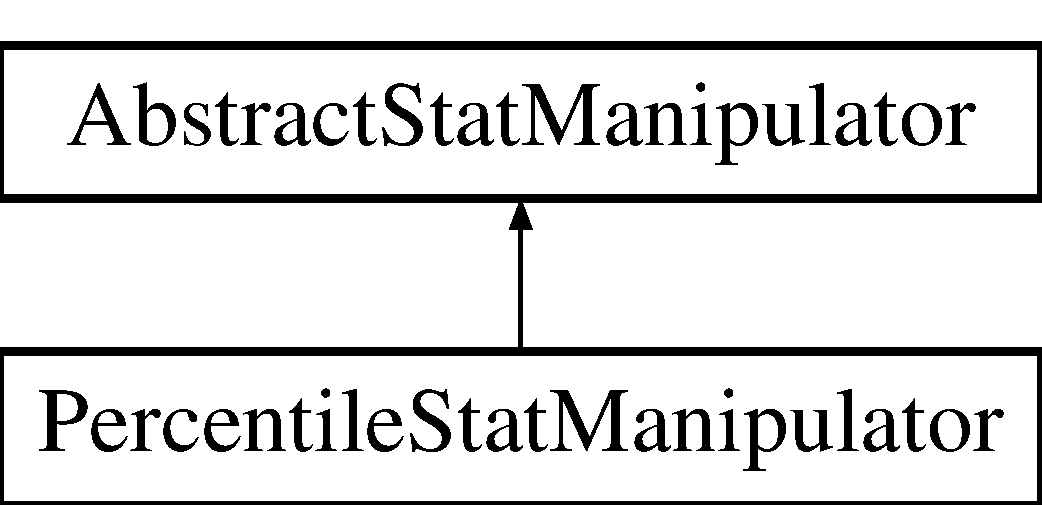
\includegraphics[height=2.000000cm]{d1/df3/class_percentile_stat_manipulator}
\end{center}
\end{figure}
\subsection*{Public Member Functions}
\begin{DoxyCompactItemize}
\item 
\hyperlink{class_percentile_stat_manipulator_abbf6cd7ebe4b1ac28ed5dd7251bd0a98}{Percentile\+Stat\+Manipulator} (int \hyperlink{class_percentile_stat_manipulator_a6a035c7f4cc7612c37486f81ef329093}{num\+Percentile})
\item 
double \hyperlink{class_percentile_stat_manipulator_aba7f8a15c5f22b5ac043e4cd97a6f8b6}{compute} (vector$<$ \hyperlink{structvessel}{vessel} $\ast$ $>$ vessels, \hyperlink{class_vessel_handler_a6cc775e9a5bcbe69ef381f56b52982e7}{Vessel\+Handler\+::\+A\+T\+T\+R\+I\+B\+U\+TE} att)
\end{DoxyCompactItemize}
\subsection*{Private Attributes}
\begin{DoxyCompactItemize}
\item 
int \hyperlink{class_percentile_stat_manipulator_a6a035c7f4cc7612c37486f81ef329093}{num\+Percentile}
\end{DoxyCompactItemize}
\subsection*{Additional Inherited Members}


\subsection{Detailed Description}
Computes the N-\/th percentile value of a specific attribute for an array of vessels. 

\subsection{Constructor \& Destructor Documentation}
\index{Percentile\+Stat\+Manipulator@{Percentile\+Stat\+Manipulator}!Percentile\+Stat\+Manipulator@{Percentile\+Stat\+Manipulator}}
\index{Percentile\+Stat\+Manipulator@{Percentile\+Stat\+Manipulator}!Percentile\+Stat\+Manipulator@{Percentile\+Stat\+Manipulator}}
\subsubsection[{\texorpdfstring{Percentile\+Stat\+Manipulator(int num\+Percentile)}{PercentileStatManipulator(int numPercentile)}}]{\setlength{\rightskip}{0pt plus 5cm}Percentile\+Stat\+Manipulator\+::\+Percentile\+Stat\+Manipulator (
\begin{DoxyParamCaption}
\item[{int}]{num\+Percentile}
\end{DoxyParamCaption}
)}\hypertarget{class_percentile_stat_manipulator_abbf6cd7ebe4b1ac28ed5dd7251bd0a98}{}\label{class_percentile_stat_manipulator_abbf6cd7ebe4b1ac28ed5dd7251bd0a98}
Constructor for the statistical manipulator 
\begin{DoxyParams}{Parameters}
{\em num\+Percentile} & Number of the percentile which the object will compute. \\
\hline
\end{DoxyParams}


\subsection{Member Function Documentation}
\index{Percentile\+Stat\+Manipulator@{Percentile\+Stat\+Manipulator}!compute@{compute}}
\index{compute@{compute}!Percentile\+Stat\+Manipulator@{Percentile\+Stat\+Manipulator}}
\subsubsection[{\texorpdfstring{compute(vector$<$ vessel $\ast$ $>$ vessels, Vessel\+Handler\+::\+A\+T\+T\+R\+I\+B\+U\+T\+E att)}{compute(vector< vessel * > vessels, VesselHandler::ATTRIBUTE att)}}]{\setlength{\rightskip}{0pt plus 5cm}double Percentile\+Stat\+Manipulator\+::compute (
\begin{DoxyParamCaption}
\item[{vector$<$ {\bf vessel} $\ast$ $>$}]{vessels, }
\item[{{\bf Vessel\+Handler\+::\+A\+T\+T\+R\+I\+B\+U\+TE}}]{att}
\end{DoxyParamCaption}
)\hspace{0.3cm}{\ttfamily [virtual]}}\hypertarget{class_percentile_stat_manipulator_aba7f8a15c5f22b5ac043e4cd97a6f8b6}{}\label{class_percentile_stat_manipulator_aba7f8a15c5f22b5ac043e4cd97a6f8b6}
Computes the statistical value of interest. 
\begin{DoxyParams}{Parameters}
{\em vessels} & Array of vessels from which the statistical function is computed. \\
\hline
\end{DoxyParams}
\begin{DoxyReturn}{Returns}
Value of the percentile. 
\end{DoxyReturn}


Implements \hyperlink{class_abstract_stat_manipulator_a8ae1dd190a2c85ff4e219a48f92763b7}{Abstract\+Stat\+Manipulator}.



\subsection{Member Data Documentation}
\index{Percentile\+Stat\+Manipulator@{Percentile\+Stat\+Manipulator}!num\+Percentile@{num\+Percentile}}
\index{num\+Percentile@{num\+Percentile}!Percentile\+Stat\+Manipulator@{Percentile\+Stat\+Manipulator}}
\subsubsection[{\texorpdfstring{num\+Percentile}{numPercentile}}]{\setlength{\rightskip}{0pt plus 5cm}int Percentile\+Stat\+Manipulator\+::num\+Percentile\hspace{0.3cm}{\ttfamily [private]}}\hypertarget{class_percentile_stat_manipulator_a6a035c7f4cc7612c37486f81ef329093}{}\label{class_percentile_stat_manipulator_a6a035c7f4cc7612c37486f81ef329093}
Number of the percentile which the object computes. 

The documentation for this class was generated from the following files\+:\begin{DoxyCompactItemize}
\item 
stats/Percentile\+Stat\+Manipulator.\+h\item 
stats/Percentile\+Stat\+Manipulator.\+cpp\end{DoxyCompactItemize}

\hypertarget{structpoint}{}\section{point Struct Reference}
\label{structpoint}\index{point@{point}}


{\ttfamily \#include $<$C\+C\+O\+Common\+Structures.\+h$>$}

\subsection*{Public Member Functions}
\begin{DoxyCompactItemize}
\item 
\mbox{\Hypertarget{structpoint_a4c712881b83fd79c9039ccdd5cb99937}\label{structpoint_a4c712881b83fd79c9039ccdd5cb99937}} 
\mbox{\hyperlink{structpoint}{point}} {\bfseries operator+} (\mbox{\hyperlink{structpoint}{point}} a)
\item 
\mbox{\Hypertarget{structpoint_a0d3ae3b14d2b34458eec85fdf10c681f}\label{structpoint_a0d3ae3b14d2b34458eec85fdf10c681f}} 
\mbox{\hyperlink{structpoint}{point}} {\bfseries operator$\ast$} (\mbox{\hyperlink{structpoint}{point}} a)
\item 
\mbox{\Hypertarget{structpoint_ac02b60d2271155b71546fadb429ff062}\label{structpoint_ac02b60d2271155b71546fadb429ff062}} 
\mbox{\hyperlink{structpoint}{point}} {\bfseries operator$\ast$} (double alpha)
\item 
\mbox{\Hypertarget{structpoint_acf04c4cee649781e93868bc1ea95e5ae}\label{structpoint_acf04c4cee649781e93868bc1ea95e5ae}} 
double {\bfseries operator$^\wedge$} (\mbox{\hyperlink{structpoint}{point}} a)
\item 
\mbox{\Hypertarget{structpoint_aeba7e4e06c7c0da9b68ebeef5f56b6df}\label{structpoint_aeba7e4e06c7c0da9b68ebeef5f56b6df}} 
\mbox{\hyperlink{structpoint}{point}} {\bfseries operator-\/} (\mbox{\hyperlink{structpoint}{point}} a)
\item 
\mbox{\Hypertarget{structpoint_a467f0c3a57bc85ab2851c4c7fd19ae9e}\label{structpoint_a467f0c3a57bc85ab2851c4c7fd19ae9e}} 
int {\bfseries operator==} (\mbox{\hyperlink{structpoint}{point}} a)
\end{DoxyCompactItemize}
\subsection*{Public Attributes}
\begin{DoxyCompactItemize}
\item 
\mbox{\Hypertarget{structpoint_a261ff1e6d38cdfae2183a88e4d8809e4}\label{structpoint_a261ff1e6d38cdfae2183a88e4d8809e4}} 
double {\bfseries p} \mbox{[}3\mbox{]}
\end{DoxyCompactItemize}


\subsection{Detailed Description}
Point structure endowed with basic linear algebra operations. 

The documentation for this struct was generated from the following file\+:\begin{DoxyCompactItemize}
\item 
structures/C\+C\+O\+Common\+Structures.\+h\end{DoxyCompactItemize}

\hypertarget{class_simple_domain}{}\section{Simple\+Domain Class Reference}
\label{class_simple_domain}\index{Simple\+Domain@{Simple\+Domain}}


{\ttfamily \#include $<$Simple\+Domain.\+h$>$}

Inheritance diagram for Simple\+Domain\+:\begin{figure}[H]
\begin{center}
\leavevmode
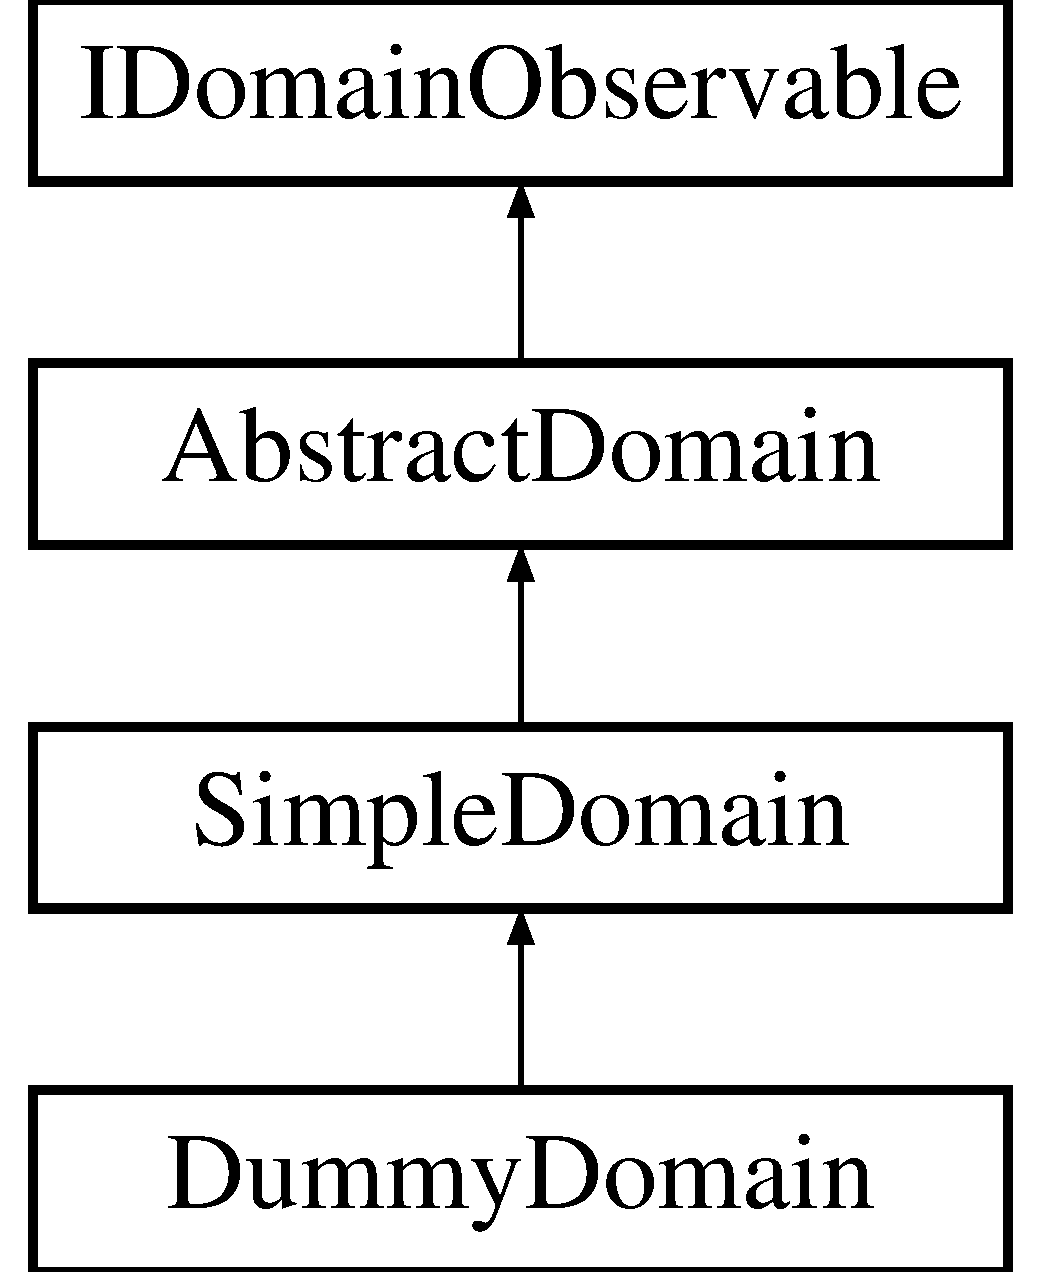
\includegraphics[height=4.000000cm]{d2/d85/class_simple_domain}
\end{center}
\end{figure}
\subsection*{Public Member Functions}
\begin{DoxyCompactItemize}
\item 
\hyperlink{class_simple_domain_a7f9767527c58a3d9a44e4267f97abf09}{Simple\+Domain} (string filename, \hyperlink{class_generator_data}{Generator\+Data} $\ast$\hyperlink{class_abstract_domain_aa37fbabc2bfa92c574f7db7544016b53}{instance\+Data})
\item 
\hyperlink{class_simple_domain_aebd1d37e199fb12d12c6763602ce80b9}{Simple\+Domain} (string filename, int \hyperlink{class_simple_domain_a3558a17833f49034ea65a9d6640403c4}{n\+Draw}, \hyperlink{class_generator_data}{Generator\+Data} $\ast$\hyperlink{class_abstract_domain_aa37fbabc2bfa92c574f7db7544016b53}{instance\+Data})
\item 
\hyperlink{class_simple_domain_a79349a46b135f855cc4942e735de5053}{Simple\+Domain} (string filename, int \hyperlink{class_simple_domain_a3558a17833f49034ea65a9d6640403c4}{n\+Draw}, int seed, \hyperlink{class_generator_data}{Generator\+Data} $\ast$\hyperlink{class_abstract_domain_aa37fbabc2bfa92c574f7db7544016b53}{instance\+Data})
\item 
\hyperlink{class_simple_domain_a53d6b37f30cf6add1978d9c06a4c509c}{Simple\+Domain} (string filename, int \hyperlink{class_simple_domain_a3558a17833f49034ea65a9d6640403c4}{n\+Draw}, int seed, \hyperlink{class_generator_data}{Generator\+Data} $\ast$\hyperlink{class_abstract_domain_aa37fbabc2bfa92c574f7db7544016b53}{instance\+Data}, \hyperlink{class_distribution_generator}{Distribution\+Generator} $\ast$\hyperlink{class_simple_domain_a522b7ae1a103ca9fe78607d5bffab4f2}{distribution})
\item 
int \hyperlink{class_simple_domain_ab1e60afe4302149098b11631d20aebb7}{is\+Segment\+Inside} (\hyperlink{structpoint}{point} xs, \hyperlink{structpoint}{point} xf)
\item 
double \hyperlink{class_simple_domain_a2a7e2919f633368b85aa3e9cfd0e57ab}{get\+Characteristic\+Length} ()
\item 
double \hyperlink{class_simple_domain_a413c188add5702b18bb838283b68bcbe}{get\+D\+Lim} (long long int n\+Vessels, double factor)
\item 
double $\ast$ \hyperlink{class_simple_domain_a0491a8bc37f8e27031f2b67b79eaf45e}{get\+Local\+Neighborhood} (\hyperlink{structpoint}{point} p, long long int n\+Vessels)
\item 
double \hyperlink{class_simple_domain_a0a05345c81234a3e616447a16e9150c0}{get\+Size} ()
\item 
virtual \hyperlink{structpoint}{point} \hyperlink{class_simple_domain_afcf98b009584217d8ab03e0dbfa86839}{get\+Random\+Point} ()
\item 
vtk\+Smart\+Pointer$<$ vtk\+O\+B\+B\+Tree $>$ \& \hyperlink{class_simple_domain_a512393f4e387bd471bbe9241e6aa28a2}{get\+Locator} ()
\item 
int \hyperlink{class_simple_domain_a25b8e92e59ae6ec5b5a463caf4d19882}{get\+Draw} ()
\item 
deque$<$ \hyperlink{structpoint}{point} $>$ \& \hyperlink{class_simple_domain_acfe3e4aeaea246579b6102707d050bf0}{get\+Random\+Inner\+Points} ()
\item 
vtk\+Smart\+Pointer$<$ vtk\+Poly\+Data $>$ \& \hyperlink{class_simple_domain_a13f9ab047e641a022648ca6468651f9f}{get\+Vtk\+Geometry} ()
\end{DoxyCompactItemize}
\subsection*{Protected Member Functions}
\begin{DoxyCompactItemize}
\item 
void {\bfseries generate\+Random\+Points} ()\hypertarget{class_simple_domain_a47fede50eae6301d9aab0024d0cc32fa}{}\label{class_simple_domain_a47fede50eae6301d9aab0024d0cc32fa}

\item 
void {\bfseries remove\+Random\+Outer\+Points} ()\hypertarget{class_simple_domain_a2d3e15dd1f43edaffc0cc11376fd4d81}{}\label{class_simple_domain_a2d3e15dd1f43edaffc0cc11376fd4d81}

\end{DoxyCompactItemize}
\subsection*{Protected Attributes}
\begin{DoxyCompactItemize}
\item 
deque$<$ \hyperlink{structpoint}{point} $>$ {\bfseries random\+Inner\+Points}\hypertarget{class_simple_domain_a7b180aaf731d5809daf149025fb553d0}{}\label{class_simple_domain_a7b180aaf731d5809daf149025fb553d0}

\end{DoxyCompactItemize}
\subsection*{Private Attributes}
\begin{DoxyCompactItemize}
\item 
vtk\+Smart\+Pointer$<$ vtk\+Poly\+Data $>$ \hyperlink{class_simple_domain_ad3ac10554a0fa1a950c8a05858b9e13d}{vtk\+Geometry}
\item 
vtk\+Smart\+Pointer$<$ vtk\+O\+B\+B\+Tree $>$ \hyperlink{class_simple_domain_af70c4b3e6786d3ec9fffa3cc25c9e59f}{locator}
\item 
double \hyperlink{class_simple_domain_a9071107204a54d35605996d7a55b0018}{characteristic\+Length}
\item 
int \hyperlink{class_simple_domain_a3558a17833f49034ea65a9d6640403c4}{n\+Draw}
\item 
\hyperlink{class_distribution_generator}{Distribution\+Generator} $\ast$ \hyperlink{class_simple_domain_a522b7ae1a103ca9fe78607d5bffab4f2}{distribution}
\end{DoxyCompactItemize}


\subsection{Detailed Description}
Class that model 3D domains with homogeneous perfusion characteristics. It deals with geometrical issues such as identify inner/outer points and segments, estimation of area/volume computation, generation of inner random points and computation of perfusion volume. 

\subsection{Constructor \& Destructor Documentation}
\index{Simple\+Domain@{Simple\+Domain}!Simple\+Domain@{Simple\+Domain}}
\index{Simple\+Domain@{Simple\+Domain}!Simple\+Domain@{Simple\+Domain}}
\subsubsection[{\texorpdfstring{Simple\+Domain(string filename, Generator\+Data $\ast$instance\+Data)}{SimpleDomain(string filename, GeneratorData *instanceData)}}]{\setlength{\rightskip}{0pt plus 5cm}Simple\+Domain\+::\+Simple\+Domain (
\begin{DoxyParamCaption}
\item[{string}]{filename, }
\item[{{\bf Generator\+Data} $\ast$}]{instance\+Data}
\end{DoxyParamCaption}
)}\hypertarget{class_simple_domain_a7f9767527c58a3d9a44e4267f97abf09}{}\label{class_simple_domain_a7f9767527c58a3d9a44e4267f97abf09}
Constructs a domain shaped by the vtk\+Polydata within {\ttfamily filename}. 
\begin{DoxyParams}{Parameters}
{\em filename} & File of the domain representation. \\
\hline
\end{DoxyParams}
\index{Simple\+Domain@{Simple\+Domain}!Simple\+Domain@{Simple\+Domain}}
\index{Simple\+Domain@{Simple\+Domain}!Simple\+Domain@{Simple\+Domain}}
\subsubsection[{\texorpdfstring{Simple\+Domain(string filename, int n\+Draw, Generator\+Data $\ast$instance\+Data)}{SimpleDomain(string filename, int nDraw, GeneratorData *instanceData)}}]{\setlength{\rightskip}{0pt plus 5cm}Simple\+Domain\+::\+Simple\+Domain (
\begin{DoxyParamCaption}
\item[{string}]{filename, }
\item[{int}]{n\+Draw, }
\item[{{\bf Generator\+Data} $\ast$}]{instance\+Data}
\end{DoxyParamCaption}
)}\hypertarget{class_simple_domain_aebd1d37e199fb12d12c6763602ce80b9}{}\label{class_simple_domain_aebd1d37e199fb12d12c6763602ce80b9}
Constructs a domain shaped by the vtk\+Polydata within {\ttfamily filename} which generates batches of {\ttfamily n\+Draw} random points each time that the domain is with no more points. 
\begin{DoxyParams}{Parameters}
{\em filename} & File of the domain representation. \\
\hline
{\em n\+Draw} & Random points generated at each batch. \\
\hline
\end{DoxyParams}
\index{Simple\+Domain@{Simple\+Domain}!Simple\+Domain@{Simple\+Domain}}
\index{Simple\+Domain@{Simple\+Domain}!Simple\+Domain@{Simple\+Domain}}
\subsubsection[{\texorpdfstring{Simple\+Domain(string filename, int n\+Draw, int seed, Generator\+Data $\ast$instance\+Data)}{SimpleDomain(string filename, int nDraw, int seed, GeneratorData *instanceData)}}]{\setlength{\rightskip}{0pt plus 5cm}Simple\+Domain\+::\+Simple\+Domain (
\begin{DoxyParamCaption}
\item[{string}]{filename, }
\item[{int}]{n\+Draw, }
\item[{int}]{seed, }
\item[{{\bf Generator\+Data} $\ast$}]{instance\+Data}
\end{DoxyParamCaption}
)}\hypertarget{class_simple_domain_a79349a46b135f855cc4942e735de5053}{}\label{class_simple_domain_a79349a46b135f855cc4942e735de5053}
Constructs a domain shaped by the vtk\+Polydata within {\ttfamily filename} which generates batches of {\ttfamily n\+Draw} random points each time that the domain is with no more points. 
\begin{DoxyParams}{Parameters}
{\em filename} & File of the domain representation. \\
\hline
{\em n\+Draw} & Random points generated at each batch. \\
\hline
{\em seed} & Seed that determine a specific random instance for the generation of points. \\
\hline
\end{DoxyParams}
\index{Simple\+Domain@{Simple\+Domain}!Simple\+Domain@{Simple\+Domain}}
\index{Simple\+Domain@{Simple\+Domain}!Simple\+Domain@{Simple\+Domain}}
\subsubsection[{\texorpdfstring{Simple\+Domain(string filename, int n\+Draw, int seed, Generator\+Data $\ast$instance\+Data, Distribution\+Generator $\ast$distribution)}{SimpleDomain(string filename, int nDraw, int seed, GeneratorData *instanceData, DistributionGenerator *distribution)}}]{\setlength{\rightskip}{0pt plus 5cm}Simple\+Domain\+::\+Simple\+Domain (
\begin{DoxyParamCaption}
\item[{string}]{filename, }
\item[{int}]{n\+Draw, }
\item[{int}]{seed, }
\item[{{\bf Generator\+Data} $\ast$}]{instance\+Data, }
\item[{{\bf Distribution\+Generator} $\ast$}]{distribution}
\end{DoxyParamCaption}
)}\hypertarget{class_simple_domain_a53d6b37f30cf6add1978d9c06a4c509c}{}\label{class_simple_domain_a53d6b37f30cf6add1978d9c06a4c509c}
Constructs a domain shaped by the vtk\+Polydata within {\ttfamily filename} which generates batches of {\ttfamily n\+Draw} random points each time that the domain is with no more points. 
\begin{DoxyParams}{Parameters}
{\em filename} & File of the domain representation. \\
\hline
{\em n\+Draw} & Random points generated at each batch. \\
\hline
{\em seed} & Seed that determine a specific random instance for the generation of points. \\
\hline
{\em instance\+Data} & Data of the current generation process. \\
\hline
{\em distribution} & Generator of terminal points following a specific distribution. \\
\hline
\end{DoxyParams}


\subsection{Member Function Documentation}
\index{Simple\+Domain@{Simple\+Domain}!get\+Characteristic\+Length@{get\+Characteristic\+Length}}
\index{get\+Characteristic\+Length@{get\+Characteristic\+Length}!Simple\+Domain@{Simple\+Domain}}
\subsubsection[{\texorpdfstring{get\+Characteristic\+Length()}{getCharacteristicLength()}}]{\setlength{\rightskip}{0pt plus 5cm}double Simple\+Domain\+::get\+Characteristic\+Length (
\begin{DoxyParamCaption}
{}
\end{DoxyParamCaption}
)\hspace{0.3cm}{\ttfamily [virtual]}}\hypertarget{class_simple_domain_a2a7e2919f633368b85aa3e9cfd0e57ab}{}\label{class_simple_domain_a2a7e2919f633368b85aa3e9cfd0e57ab}
Estimates a characteristic length for the current domain. This length is useful to estimate the perfusion volume of the domain. \begin{DoxyReturn}{Returns}
Chracteristic length. 
\end{DoxyReturn}


Implements \hyperlink{class_abstract_domain_a90ca3dff64bab2428da8ced24e16f4c3}{Abstract\+Domain}.

\index{Simple\+Domain@{Simple\+Domain}!get\+D\+Lim@{get\+D\+Lim}}
\index{get\+D\+Lim@{get\+D\+Lim}!Simple\+Domain@{Simple\+Domain}}
\subsubsection[{\texorpdfstring{get\+D\+Lim(long long int n\+Vessels, double factor)}{getDLim(long long int nVessels, double factor)}}]{\setlength{\rightskip}{0pt plus 5cm}double Simple\+Domain\+::get\+D\+Lim (
\begin{DoxyParamCaption}
\item[{long long int}]{n\+Vessels, }
\item[{double}]{factor}
\end{DoxyParamCaption}
)\hspace{0.3cm}{\ttfamily [virtual]}}\hypertarget{class_simple_domain_a413c188add5702b18bb838283b68bcbe}{}\label{class_simple_domain_a413c188add5702b18bb838283b68bcbe}
Minimum distance between a new vessel terminal and the tree based on the current terminal perfusion. This is lower bound criteria for the vessel length and also aids toward a spatially homogeneous terminal distribution. 
\begin{DoxyParams}{Parameters}
{\em n\+Vessels} & Quantity of terminals in the current tree. \\
\hline
{\em factor} & Factor used to scale a perfusion measure in order to estimate the D\+Lim value. \\
\hline
\end{DoxyParams}
\begin{DoxyReturn}{Returns}
D\+Lim value. 
\end{DoxyReturn}


Implements \hyperlink{class_abstract_domain_ac9f39c12182608eb704c051e5d1cbc55}{Abstract\+Domain}.

\index{Simple\+Domain@{Simple\+Domain}!get\+Draw@{get\+Draw}}
\index{get\+Draw@{get\+Draw}!Simple\+Domain@{Simple\+Domain}}
\subsubsection[{\texorpdfstring{get\+Draw()}{getDraw()}}]{\setlength{\rightskip}{0pt plus 5cm}int Simple\+Domain\+::get\+Draw (
\begin{DoxyParamCaption}
{}
\end{DoxyParamCaption}
)}\hypertarget{class_simple_domain_a25b8e92e59ae6ec5b5a463caf4d19882}{}\label{class_simple_domain_a25b8e92e59ae6ec5b5a463caf4d19882}
Returns the number of random points created in each batch of random generations. \begin{DoxyReturn}{Returns}
Number of random points created in each batch of random generations. 
\end{DoxyReturn}
\index{Simple\+Domain@{Simple\+Domain}!get\+Local\+Neighborhood@{get\+Local\+Neighborhood}}
\index{get\+Local\+Neighborhood@{get\+Local\+Neighborhood}!Simple\+Domain@{Simple\+Domain}}
\subsubsection[{\texorpdfstring{get\+Local\+Neighborhood(point p, long long int n\+Vessels)}{getLocalNeighborhood(point p, long long int nVessels)}}]{\setlength{\rightskip}{0pt plus 5cm}double $\ast$ Simple\+Domain\+::get\+Local\+Neighborhood (
\begin{DoxyParamCaption}
\item[{{\bf point}}]{p, }
\item[{long long int}]{n\+Vessels}
\end{DoxyParamCaption}
)\hspace{0.3cm}{\ttfamily [virtual]}}\hypertarget{class_simple_domain_a0491a8bc37f8e27031f2b67b79eaf45e}{}\label{class_simple_domain_a0491a8bc37f8e27031f2b67b79eaf45e}
Returns the local neighbors to the {\ttfamily p} point locus. The amount of neighbors is estimated based on the current terminal perfusion. 
\begin{DoxyParams}{Parameters}
{\em p} & Central point of the neighborhood. \\
\hline
{\em n\+Vessels} & Amount of terminals in the tree. \\
\hline
\end{DoxyParams}
\begin{DoxyReturn}{Returns}
Array of neighbor vessels. 
\end{DoxyReturn}


Implements \hyperlink{class_abstract_domain_aee2b549d19062b261429f8a442fb4714}{Abstract\+Domain}.

\index{Simple\+Domain@{Simple\+Domain}!get\+Locator@{get\+Locator}}
\index{get\+Locator@{get\+Locator}!Simple\+Domain@{Simple\+Domain}}
\subsubsection[{\texorpdfstring{get\+Locator()}{getLocator()}}]{\setlength{\rightskip}{0pt plus 5cm}vtk\+Smart\+Pointer$<$ vtk\+O\+B\+B\+Tree $>$ \& Simple\+Domain\+::get\+Locator (
\begin{DoxyParamCaption}
{}
\end{DoxyParamCaption}
)}\hypertarget{class_simple_domain_a512393f4e387bd471bbe9241e6aa28a2}{}\label{class_simple_domain_a512393f4e387bd471bbe9241e6aa28a2}
Returns the locator used to test inside segments. \begin{DoxyReturn}{Returns}
Locator used to test inside segments. 
\end{DoxyReturn}
\index{Simple\+Domain@{Simple\+Domain}!get\+Random\+Inner\+Points@{get\+Random\+Inner\+Points}}
\index{get\+Random\+Inner\+Points@{get\+Random\+Inner\+Points}!Simple\+Domain@{Simple\+Domain}}
\subsubsection[{\texorpdfstring{get\+Random\+Inner\+Points()}{getRandomInnerPoints()}}]{\setlength{\rightskip}{0pt plus 5cm}deque$<$ {\bf point} $>$ \& Simple\+Domain\+::get\+Random\+Inner\+Points (
\begin{DoxyParamCaption}
{}
\end{DoxyParamCaption}
)\hspace{0.3cm}{\ttfamily [virtual]}}\hypertarget{class_simple_domain_acfe3e4aeaea246579b6102707d050bf0}{}\label{class_simple_domain_acfe3e4aeaea246579b6102707d050bf0}
Return a set of inner domain points. \begin{DoxyReturn}{Returns}
Set of inner domain points. 
\end{DoxyReturn}


Implements \hyperlink{class_abstract_domain_a73d2c0e7c670b007bb5dbbdab5ad6b1b}{Abstract\+Domain}.

\index{Simple\+Domain@{Simple\+Domain}!get\+Random\+Point@{get\+Random\+Point}}
\index{get\+Random\+Point@{get\+Random\+Point}!Simple\+Domain@{Simple\+Domain}}
\subsubsection[{\texorpdfstring{get\+Random\+Point()}{getRandomPoint()}}]{\setlength{\rightskip}{0pt plus 5cm}{\bf point} Simple\+Domain\+::get\+Random\+Point (
\begin{DoxyParamCaption}
{}
\end{DoxyParamCaption}
)\hspace{0.3cm}{\ttfamily [virtual]}}\hypertarget{class_simple_domain_afcf98b009584217d8ab03e0dbfa86839}{}\label{class_simple_domain_afcf98b009584217d8ab03e0dbfa86839}
Return a random point inside the domain. \begin{DoxyReturn}{Returns}
Point inside the domain. 
\end{DoxyReturn}


Implements \hyperlink{class_abstract_domain_ae31a5b26d1dc628abe24da7a4d375415}{Abstract\+Domain}.



Reimplemented in \hyperlink{class_dummy_domain_a72074e5e3e53028ec4b73bffee1ba229}{Dummy\+Domain}.

\index{Simple\+Domain@{Simple\+Domain}!get\+Size@{get\+Size}}
\index{get\+Size@{get\+Size}!Simple\+Domain@{Simple\+Domain}}
\subsubsection[{\texorpdfstring{get\+Size()}{getSize()}}]{\setlength{\rightskip}{0pt plus 5cm}double Simple\+Domain\+::get\+Size (
\begin{DoxyParamCaption}
{}
\end{DoxyParamCaption}
)\hspace{0.3cm}{\ttfamily [virtual]}}\hypertarget{class_simple_domain_a0a05345c81234a3e616447a16e9150c0}{}\label{class_simple_domain_a0a05345c81234a3e616447a16e9150c0}
Computes the size of the domain. \begin{DoxyReturn}{Returns}
Size of the domain. 
\end{DoxyReturn}


Implements \hyperlink{class_abstract_domain_a049564d82f2c177c39834dfc8da143dc}{Abstract\+Domain}.

\index{Simple\+Domain@{Simple\+Domain}!get\+Vtk\+Geometry@{get\+Vtk\+Geometry}}
\index{get\+Vtk\+Geometry@{get\+Vtk\+Geometry}!Simple\+Domain@{Simple\+Domain}}
\subsubsection[{\texorpdfstring{get\+Vtk\+Geometry()}{getVtkGeometry()}}]{\setlength{\rightskip}{0pt plus 5cm}vtk\+Smart\+Pointer$<$ vtk\+Poly\+Data $>$ \& Simple\+Domain\+::get\+Vtk\+Geometry (
\begin{DoxyParamCaption}
{}
\end{DoxyParamCaption}
)\hspace{0.3cm}{\ttfamily [virtual]}}\hypertarget{class_simple_domain_a13f9ab047e641a022648ca6468651f9f}{}\label{class_simple_domain_a13f9ab047e641a022648ca6468651f9f}
Returns the vtk\+Polydata with the domain representation. \begin{DoxyReturn}{Returns}
vtk\+Polydata with the domain representation. 
\end{DoxyReturn}


Implements \hyperlink{class_abstract_domain_abb1e386d2899cb6b725509259a836cd0}{Abstract\+Domain}.

\index{Simple\+Domain@{Simple\+Domain}!is\+Segment\+Inside@{is\+Segment\+Inside}}
\index{is\+Segment\+Inside@{is\+Segment\+Inside}!Simple\+Domain@{Simple\+Domain}}
\subsubsection[{\texorpdfstring{is\+Segment\+Inside(point xs, point xf)}{isSegmentInside(point xs, point xf)}}]{\setlength{\rightskip}{0pt plus 5cm}int Simple\+Domain\+::is\+Segment\+Inside (
\begin{DoxyParamCaption}
\item[{{\bf point}}]{xs, }
\item[{{\bf point}}]{xf}
\end{DoxyParamCaption}
)\hspace{0.3cm}{\ttfamily [virtual]}}\hypertarget{class_simple_domain_ab1e60afe4302149098b11631d20aebb7}{}\label{class_simple_domain_ab1e60afe4302149098b11631d20aebb7}
Returns if the segment defined by the vertexes {\ttfamily xs} and {\ttfamily xf} is inside the current domain. 
\begin{DoxyParams}{Parameters}
{\em xs} & Start point of the segment. \\
\hline
{\em xf} & End point of the segment. \\
\hline
\end{DoxyParams}
\begin{DoxyReturn}{Returns}
1 if the segment defined by the vertexes {\ttfamily xs} and {\ttfamily xf} is inside the current domain otherwise 0. 
\end{DoxyReturn}


Implements \hyperlink{class_abstract_domain_a8544eef21fb6700ecc02e9cd50884efd}{Abstract\+Domain}.



\subsection{Member Data Documentation}
\index{Simple\+Domain@{Simple\+Domain}!characteristic\+Length@{characteristic\+Length}}
\index{characteristic\+Length@{characteristic\+Length}!Simple\+Domain@{Simple\+Domain}}
\subsubsection[{\texorpdfstring{characteristic\+Length}{characteristicLength}}]{\setlength{\rightskip}{0pt plus 5cm}double Simple\+Domain\+::characteristic\+Length\hspace{0.3cm}{\ttfamily [private]}}\hypertarget{class_simple_domain_a9071107204a54d35605996d7a55b0018}{}\label{class_simple_domain_a9071107204a54d35605996d7a55b0018}
Characteristic length for the domain. \index{Simple\+Domain@{Simple\+Domain}!distribution@{distribution}}
\index{distribution@{distribution}!Simple\+Domain@{Simple\+Domain}}
\subsubsection[{\texorpdfstring{distribution}{distribution}}]{\setlength{\rightskip}{0pt plus 5cm}{\bf Distribution\+Generator}$\ast$ Simple\+Domain\+::distribution\hspace{0.3cm}{\ttfamily [private]}}\hypertarget{class_simple_domain_a522b7ae1a103ca9fe78607d5bffab4f2}{}\label{class_simple_domain_a522b7ae1a103ca9fe78607d5bffab4f2}
Point generator \index{Simple\+Domain@{Simple\+Domain}!locator@{locator}}
\index{locator@{locator}!Simple\+Domain@{Simple\+Domain}}
\subsubsection[{\texorpdfstring{locator}{locator}}]{\setlength{\rightskip}{0pt plus 5cm}vtk\+Smart\+Pointer$<$vtk\+O\+B\+B\+Tree$>$ Simple\+Domain\+::locator\hspace{0.3cm}{\ttfamily [private]}}\hypertarget{class_simple_domain_af70c4b3e6786d3ec9fffa3cc25c9e59f}{}\label{class_simple_domain_af70c4b3e6786d3ec9fffa3cc25c9e59f}
Cell locator responsible to determine if a segment is inside the domain. \index{Simple\+Domain@{Simple\+Domain}!n\+Draw@{n\+Draw}}
\index{n\+Draw@{n\+Draw}!Simple\+Domain@{Simple\+Domain}}
\subsubsection[{\texorpdfstring{n\+Draw}{nDraw}}]{\setlength{\rightskip}{0pt plus 5cm}int Simple\+Domain\+::n\+Draw\hspace{0.3cm}{\ttfamily [private]}}\hypertarget{class_simple_domain_a3558a17833f49034ea65a9d6640403c4}{}\label{class_simple_domain_a3558a17833f49034ea65a9d6640403c4}
Amount of points randomly generated when no more points are available. \index{Simple\+Domain@{Simple\+Domain}!vtk\+Geometry@{vtk\+Geometry}}
\index{vtk\+Geometry@{vtk\+Geometry}!Simple\+Domain@{Simple\+Domain}}
\subsubsection[{\texorpdfstring{vtk\+Geometry}{vtkGeometry}}]{\setlength{\rightskip}{0pt plus 5cm}vtk\+Smart\+Pointer$<$vtk\+Poly\+Data$>$ Simple\+Domain\+::vtk\+Geometry\hspace{0.3cm}{\ttfamily [private]}}\hypertarget{class_simple_domain_ad3ac10554a0fa1a950c8a05858b9e13d}{}\label{class_simple_domain_ad3ac10554a0fa1a950c8a05858b9e13d}
vtk\+Polydata description of the domain. 

The documentation for this class was generated from the following files\+:\begin{DoxyCompactItemize}
\item 
structures/domain/Simple\+Domain.\+h\item 
structures/domain/Simple\+Domain.\+cpp\end{DoxyCompactItemize}

\hypertarget{class_simple_domain2_d}{}\section{Simple\+Domain2D Class Reference}
\label{class_simple_domain2_d}\index{Simple\+Domain2D@{Simple\+Domain2D}}


{\ttfamily \#include $<$Simple\+Domain2\+D.\+h$>$}

Inheritance diagram for Simple\+Domain2D\+:\begin{figure}[H]
\begin{center}
\leavevmode
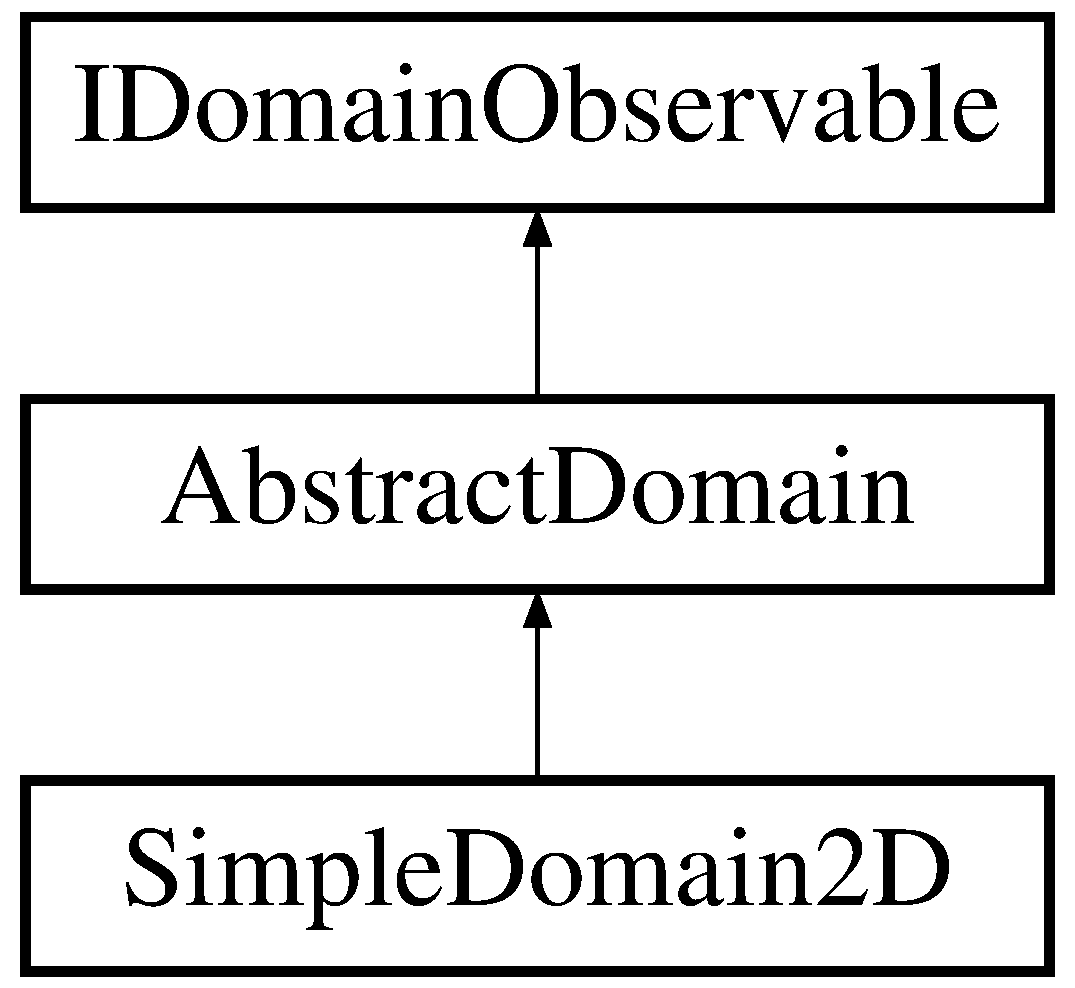
\includegraphics[height=3.000000cm]{dd/dd9/class_simple_domain2_d}
\end{center}
\end{figure}
\subsection*{Public Member Functions}
\begin{DoxyCompactItemize}
\item 
\hyperlink{class_simple_domain2_d_a08c1cec51a7bc1d3cc7e65f8f1346bef}{Simple\+Domain2D} (string filename, \hyperlink{class_generator_data}{Generator\+Data} $\ast$\hyperlink{class_abstract_domain_aa37fbabc2bfa92c574f7db7544016b53}{instance\+Data})
\item 
\hyperlink{class_simple_domain2_d_a52afa98107cdf2888d4ce006354b53d9}{Simple\+Domain2D} (string filename, int \hyperlink{class_simple_domain2_d_ad541f350ae7423116545f4363f8d0715}{n\+Draw}, \hyperlink{class_generator_data}{Generator\+Data} $\ast$\hyperlink{class_abstract_domain_aa37fbabc2bfa92c574f7db7544016b53}{instance\+Data})
\item 
\hyperlink{class_simple_domain2_d_ad36b389b52d7341010d181986de0b9a0}{Simple\+Domain2D} (string filename, int \hyperlink{class_simple_domain2_d_ad541f350ae7423116545f4363f8d0715}{n\+Draw}, int \hyperlink{class_simple_domain2_d_abca10a88602d74c02d5d94651d9fc8bd}{seed}, \hyperlink{class_generator_data}{Generator\+Data} $\ast$\hyperlink{class_abstract_domain_aa37fbabc2bfa92c574f7db7544016b53}{instance\+Data})
\item 
int \hyperlink{class_simple_domain2_d_a18706cdbe4f61a71eceb7257fd4ec6dd}{is\+Segment\+Inside} (\hyperlink{structpoint}{point} xs, \hyperlink{structpoint}{point} xf)
\item 
double \hyperlink{class_simple_domain2_d_a5bf4df64fe80dae1e394b2f2c73c3d05}{get\+Characteristic\+Length} ()
\item 
double \hyperlink{class_simple_domain2_d_a60dbee1351f604d7ee61121d923de823}{get\+D\+Lim} (long long int n\+Vessels, double factor)
\item 
double $\ast$ \hyperlink{class_simple_domain2_d_a5c7eaa0e32e25950149c4735bd02c671}{get\+Local\+Neighborhood} (\hyperlink{structpoint}{point} p, long long int n\+Vessels)
\item 
double \hyperlink{class_simple_domain2_d_ad5e1ba1529fd8088f64af603cc5c18a3}{get\+Size} ()
\item 
virtual \hyperlink{structpoint}{point} \hyperlink{class_simple_domain2_d_a8b19e2fa69a0f13813b0296f270f11e9}{get\+Random\+Point} ()
\item 
vtk\+Smart\+Pointer$<$ vtk\+O\+B\+B\+Tree $>$ \& \hyperlink{class_simple_domain2_d_a09fc603691f205b49d975aab902cdef4}{get\+Locator} ()
\item 
int \hyperlink{class_simple_domain2_d_a15b519453137710f0c8897a4eda7c25d}{get\+Draw} ()
\item 
deque$<$ \hyperlink{structpoint}{point} $>$ \& \hyperlink{class_simple_domain2_d_a08eddf131c1ed43cf7cc34e347fd372f}{get\+Random\+Inner\+Points} ()
\item 
vtk\+Smart\+Pointer$<$ vtk\+Poly\+Data $>$ \& \hyperlink{class_simple_domain2_d_a0c4505e70d9530586bcb0ab943bb9a9a}{get\+Vtk\+Geometry} ()
\end{DoxyCompactItemize}
\subsection*{Protected Member Functions}
\begin{DoxyCompactItemize}
\item 
void {\bfseries generate\+Random\+Points} ()\hypertarget{class_simple_domain2_d_aeeb59155f6dec3e57e515c4b3a703e08}{}\label{class_simple_domain2_d_aeeb59155f6dec3e57e515c4b3a703e08}

\item 
void {\bfseries remove\+Random\+Outer\+Points\+Serial} ()\hypertarget{class_simple_domain2_d_af1cab33fce288f46723cb7860f7ed8bb}{}\label{class_simple_domain2_d_af1cab33fce288f46723cb7860f7ed8bb}

\item 
void {\bfseries remove\+Random\+Outer\+Points} ()\hypertarget{class_simple_domain2_d_af4f587398d458be9dfb09e47abfc3ad9}{}\label{class_simple_domain2_d_af4f587398d458be9dfb09e47abfc3ad9}

\end{DoxyCompactItemize}
\subsection*{Protected Attributes}
\begin{DoxyCompactItemize}
\item 
deque$<$ \hyperlink{structpoint}{point} $>$ {\bfseries random\+Inner\+Points}\hypertarget{class_simple_domain2_d_a3baccded48c6c2d227c86938639c7e3b}{}\label{class_simple_domain2_d_a3baccded48c6c2d227c86938639c7e3b}

\end{DoxyCompactItemize}
\subsection*{Private Attributes}
\begin{DoxyCompactItemize}
\item 
vtk\+Smart\+Pointer$<$ vtk\+Poly\+Data $>$ \hyperlink{class_simple_domain2_d_a2acccf092aaaccfc4fabcd7668a4cc32}{vtk\+Geometry}
\item 
vtk\+Smart\+Pointer$<$ vtk\+O\+B\+B\+Tree $>$ \hyperlink{class_simple_domain2_d_a663886e5e4f47a4d1cec260c93b2498b}{locator}
\item 
double \hyperlink{class_simple_domain2_d_a3504bd60c2e2585bd28f9bac63e6eee7}{characteristic\+Length}
\item 
int \hyperlink{class_simple_domain2_d_ad541f350ae7423116545f4363f8d0715}{n\+Draw}
\item 
int \hyperlink{class_simple_domain2_d_abca10a88602d74c02d5d94651d9fc8bd}{seed} = -\/1
\item 
mt19937 \hyperlink{class_simple_domain2_d_a752e854a584a9bc6476903d639d8c0ed}{generator}
\end{DoxyCompactItemize}


\subsection{Detailed Description}
Class that model 2D (sheet-\/like) domains with homogeneous perfusion characteristics. It deals with geometrical issues such as identify inner/outer points and segments, estimation of area/volume computation, generation of inner random points and computation of perfusion volume. 

\subsection{Constructor \& Destructor Documentation}
\index{Simple\+Domain2D@{Simple\+Domain2D}!Simple\+Domain2D@{Simple\+Domain2D}}
\index{Simple\+Domain2D@{Simple\+Domain2D}!Simple\+Domain2D@{Simple\+Domain2D}}
\subsubsection[{\texorpdfstring{Simple\+Domain2\+D(string filename, Generator\+Data $\ast$instance\+Data)}{SimpleDomain2D(string filename, GeneratorData *instanceData)}}]{\setlength{\rightskip}{0pt plus 5cm}Simple\+Domain2\+D\+::\+Simple\+Domain2D (
\begin{DoxyParamCaption}
\item[{string}]{filename, }
\item[{{\bf Generator\+Data} $\ast$}]{instance\+Data}
\end{DoxyParamCaption}
)}\hypertarget{class_simple_domain2_d_a08c1cec51a7bc1d3cc7e65f8f1346bef}{}\label{class_simple_domain2_d_a08c1cec51a7bc1d3cc7e65f8f1346bef}
Constructs a domain shaped by the vtk\+Polydata within {\ttfamily filename}. 
\begin{DoxyParams}{Parameters}
{\em filename} & File of the domain representation. \\
\hline
\end{DoxyParams}
\index{Simple\+Domain2D@{Simple\+Domain2D}!Simple\+Domain2D@{Simple\+Domain2D}}
\index{Simple\+Domain2D@{Simple\+Domain2D}!Simple\+Domain2D@{Simple\+Domain2D}}
\subsubsection[{\texorpdfstring{Simple\+Domain2\+D(string filename, int n\+Draw, Generator\+Data $\ast$instance\+Data)}{SimpleDomain2D(string filename, int nDraw, GeneratorData *instanceData)}}]{\setlength{\rightskip}{0pt plus 5cm}Simple\+Domain2\+D\+::\+Simple\+Domain2D (
\begin{DoxyParamCaption}
\item[{string}]{filename, }
\item[{int}]{n\+Draw, }
\item[{{\bf Generator\+Data} $\ast$}]{instance\+Data}
\end{DoxyParamCaption}
)}\hypertarget{class_simple_domain2_d_a52afa98107cdf2888d4ce006354b53d9}{}\label{class_simple_domain2_d_a52afa98107cdf2888d4ce006354b53d9}
Constructs a domain shaped by the vtk\+Polydata within {\ttfamily filename} which generates batches of {\ttfamily n\+Draw} random points each time that the domain is with no more points. 
\begin{DoxyParams}{Parameters}
{\em filename} & File of the domain representation. \\
\hline
{\em n\+Draw} & Random points generated at each batch. \\
\hline
\end{DoxyParams}
\index{Simple\+Domain2D@{Simple\+Domain2D}!Simple\+Domain2D@{Simple\+Domain2D}}
\index{Simple\+Domain2D@{Simple\+Domain2D}!Simple\+Domain2D@{Simple\+Domain2D}}
\subsubsection[{\texorpdfstring{Simple\+Domain2\+D(string filename, int n\+Draw, int seed, Generator\+Data $\ast$instance\+Data)}{SimpleDomain2D(string filename, int nDraw, int seed, GeneratorData *instanceData)}}]{\setlength{\rightskip}{0pt plus 5cm}Simple\+Domain2\+D\+::\+Simple\+Domain2D (
\begin{DoxyParamCaption}
\item[{string}]{filename, }
\item[{int}]{n\+Draw, }
\item[{int}]{seed, }
\item[{{\bf Generator\+Data} $\ast$}]{instance\+Data}
\end{DoxyParamCaption}
)}\hypertarget{class_simple_domain2_d_ad36b389b52d7341010d181986de0b9a0}{}\label{class_simple_domain2_d_ad36b389b52d7341010d181986de0b9a0}
Constructs a domain shaped by the vtk\+Polydata within {\ttfamily filename} which generates batches of {\ttfamily n\+Draw} random points each time that the domain is with no more points. 
\begin{DoxyParams}{Parameters}
{\em filename} & File of the domain representation. \\
\hline
{\em n\+Draw} & Random points generated at each batch. \\
\hline
{\em seed} & Seed that determine a specific random instance for the generation of points. \\
\hline
\end{DoxyParams}


\subsection{Member Function Documentation}
\index{Simple\+Domain2D@{Simple\+Domain2D}!get\+Characteristic\+Length@{get\+Characteristic\+Length}}
\index{get\+Characteristic\+Length@{get\+Characteristic\+Length}!Simple\+Domain2D@{Simple\+Domain2D}}
\subsubsection[{\texorpdfstring{get\+Characteristic\+Length()}{getCharacteristicLength()}}]{\setlength{\rightskip}{0pt plus 5cm}double Simple\+Domain2\+D\+::get\+Characteristic\+Length (
\begin{DoxyParamCaption}
{}
\end{DoxyParamCaption}
)\hspace{0.3cm}{\ttfamily [virtual]}}\hypertarget{class_simple_domain2_d_a5bf4df64fe80dae1e394b2f2c73c3d05}{}\label{class_simple_domain2_d_a5bf4df64fe80dae1e394b2f2c73c3d05}
Estimates a characteristic length for the current domain. This length is useful to estimate the perfusion volume of the domain. \begin{DoxyReturn}{Returns}
Chracteristic length. 
\end{DoxyReturn}


Implements \hyperlink{class_abstract_domain_a90ca3dff64bab2428da8ced24e16f4c3}{Abstract\+Domain}.

\index{Simple\+Domain2D@{Simple\+Domain2D}!get\+D\+Lim@{get\+D\+Lim}}
\index{get\+D\+Lim@{get\+D\+Lim}!Simple\+Domain2D@{Simple\+Domain2D}}
\subsubsection[{\texorpdfstring{get\+D\+Lim(long long int n\+Vessels, double factor)}{getDLim(long long int nVessels, double factor)}}]{\setlength{\rightskip}{0pt plus 5cm}double Simple\+Domain2\+D\+::get\+D\+Lim (
\begin{DoxyParamCaption}
\item[{long long int}]{n\+Vessels, }
\item[{double}]{factor}
\end{DoxyParamCaption}
)\hspace{0.3cm}{\ttfamily [virtual]}}\hypertarget{class_simple_domain2_d_a60dbee1351f604d7ee61121d923de823}{}\label{class_simple_domain2_d_a60dbee1351f604d7ee61121d923de823}
Minimum distance between a new vessel terminal and the tree based on the current terminal perfusion. This is lower bound criteria for the vessel length and also aids toward a spatially homogeneous terminal distribution. 
\begin{DoxyParams}{Parameters}
{\em n\+Vessels} & Quantity of terminals in the current tree. \\
\hline
{\em factor} & Factor used to scale a perfusion measure in order to estimate the D\+Lim value. \\
\hline
\end{DoxyParams}
\begin{DoxyReturn}{Returns}
D\+Lim value. 
\end{DoxyReturn}


Implements \hyperlink{class_abstract_domain_ac9f39c12182608eb704c051e5d1cbc55}{Abstract\+Domain}.

\index{Simple\+Domain2D@{Simple\+Domain2D}!get\+Draw@{get\+Draw}}
\index{get\+Draw@{get\+Draw}!Simple\+Domain2D@{Simple\+Domain2D}}
\subsubsection[{\texorpdfstring{get\+Draw()}{getDraw()}}]{\setlength{\rightskip}{0pt plus 5cm}int Simple\+Domain2\+D\+::get\+Draw (
\begin{DoxyParamCaption}
{}
\end{DoxyParamCaption}
)}\hypertarget{class_simple_domain2_d_a15b519453137710f0c8897a4eda7c25d}{}\label{class_simple_domain2_d_a15b519453137710f0c8897a4eda7c25d}
Returns the number of random points created in each batch of random generations. \begin{DoxyReturn}{Returns}
Number of random points created in each batch of random generations. 
\end{DoxyReturn}
\index{Simple\+Domain2D@{Simple\+Domain2D}!get\+Local\+Neighborhood@{get\+Local\+Neighborhood}}
\index{get\+Local\+Neighborhood@{get\+Local\+Neighborhood}!Simple\+Domain2D@{Simple\+Domain2D}}
\subsubsection[{\texorpdfstring{get\+Local\+Neighborhood(point p, long long int n\+Vessels)}{getLocalNeighborhood(point p, long long int nVessels)}}]{\setlength{\rightskip}{0pt plus 5cm}double $\ast$ Simple\+Domain2\+D\+::get\+Local\+Neighborhood (
\begin{DoxyParamCaption}
\item[{{\bf point}}]{p, }
\item[{long long int}]{n\+Vessels}
\end{DoxyParamCaption}
)\hspace{0.3cm}{\ttfamily [virtual]}}\hypertarget{class_simple_domain2_d_a5c7eaa0e32e25950149c4735bd02c671}{}\label{class_simple_domain2_d_a5c7eaa0e32e25950149c4735bd02c671}
Returns the local neighbors to the {\ttfamily p} point locus. The amount of neighbors is estimated based on the current terminal perfusion. 
\begin{DoxyParams}{Parameters}
{\em p} & Central point of the neighborhood. \\
\hline
{\em n\+Vessels} & Amount of terminals in the tree. \\
\hline
\end{DoxyParams}
\begin{DoxyReturn}{Returns}
Array of neighbor vessels. 
\end{DoxyReturn}


Implements \hyperlink{class_abstract_domain_aee2b549d19062b261429f8a442fb4714}{Abstract\+Domain}.

\index{Simple\+Domain2D@{Simple\+Domain2D}!get\+Locator@{get\+Locator}}
\index{get\+Locator@{get\+Locator}!Simple\+Domain2D@{Simple\+Domain2D}}
\subsubsection[{\texorpdfstring{get\+Locator()}{getLocator()}}]{\setlength{\rightskip}{0pt plus 5cm}vtk\+Smart\+Pointer$<$ vtk\+O\+B\+B\+Tree $>$ \& Simple\+Domain2\+D\+::get\+Locator (
\begin{DoxyParamCaption}
{}
\end{DoxyParamCaption}
)}\hypertarget{class_simple_domain2_d_a09fc603691f205b49d975aab902cdef4}{}\label{class_simple_domain2_d_a09fc603691f205b49d975aab902cdef4}
Returns the locator used to test inside segments. \begin{DoxyReturn}{Returns}
Locator used to test inside segments. 
\end{DoxyReturn}
\index{Simple\+Domain2D@{Simple\+Domain2D}!get\+Random\+Inner\+Points@{get\+Random\+Inner\+Points}}
\index{get\+Random\+Inner\+Points@{get\+Random\+Inner\+Points}!Simple\+Domain2D@{Simple\+Domain2D}}
\subsubsection[{\texorpdfstring{get\+Random\+Inner\+Points()}{getRandomInnerPoints()}}]{\setlength{\rightskip}{0pt plus 5cm}deque$<$ {\bf point} $>$ \& Simple\+Domain2\+D\+::get\+Random\+Inner\+Points (
\begin{DoxyParamCaption}
{}
\end{DoxyParamCaption}
)\hspace{0.3cm}{\ttfamily [virtual]}}\hypertarget{class_simple_domain2_d_a08eddf131c1ed43cf7cc34e347fd372f}{}\label{class_simple_domain2_d_a08eddf131c1ed43cf7cc34e347fd372f}
Return a set of inner domain points. \begin{DoxyReturn}{Returns}
Set of inner domain points. 
\end{DoxyReturn}


Implements \hyperlink{class_abstract_domain_a73d2c0e7c670b007bb5dbbdab5ad6b1b}{Abstract\+Domain}.

\index{Simple\+Domain2D@{Simple\+Domain2D}!get\+Random\+Point@{get\+Random\+Point}}
\index{get\+Random\+Point@{get\+Random\+Point}!Simple\+Domain2D@{Simple\+Domain2D}}
\subsubsection[{\texorpdfstring{get\+Random\+Point()}{getRandomPoint()}}]{\setlength{\rightskip}{0pt plus 5cm}{\bf point} Simple\+Domain2\+D\+::get\+Random\+Point (
\begin{DoxyParamCaption}
{}
\end{DoxyParamCaption}
)\hspace{0.3cm}{\ttfamily [virtual]}}\hypertarget{class_simple_domain2_d_a8b19e2fa69a0f13813b0296f270f11e9}{}\label{class_simple_domain2_d_a8b19e2fa69a0f13813b0296f270f11e9}
Return a random point inside the domain. \begin{DoxyReturn}{Returns}
Point inside the domain. 
\end{DoxyReturn}


Implements \hyperlink{class_abstract_domain_ae31a5b26d1dc628abe24da7a4d375415}{Abstract\+Domain}.

\index{Simple\+Domain2D@{Simple\+Domain2D}!get\+Size@{get\+Size}}
\index{get\+Size@{get\+Size}!Simple\+Domain2D@{Simple\+Domain2D}}
\subsubsection[{\texorpdfstring{get\+Size()}{getSize()}}]{\setlength{\rightskip}{0pt plus 5cm}double Simple\+Domain2\+D\+::get\+Size (
\begin{DoxyParamCaption}
{}
\end{DoxyParamCaption}
)\hspace{0.3cm}{\ttfamily [virtual]}}\hypertarget{class_simple_domain2_d_ad5e1ba1529fd8088f64af603cc5c18a3}{}\label{class_simple_domain2_d_ad5e1ba1529fd8088f64af603cc5c18a3}
Computes the size of the domain. \begin{DoxyReturn}{Returns}
Size of the domain. 
\end{DoxyReturn}


Implements \hyperlink{class_abstract_domain_a049564d82f2c177c39834dfc8da143dc}{Abstract\+Domain}.

\index{Simple\+Domain2D@{Simple\+Domain2D}!get\+Vtk\+Geometry@{get\+Vtk\+Geometry}}
\index{get\+Vtk\+Geometry@{get\+Vtk\+Geometry}!Simple\+Domain2D@{Simple\+Domain2D}}
\subsubsection[{\texorpdfstring{get\+Vtk\+Geometry()}{getVtkGeometry()}}]{\setlength{\rightskip}{0pt plus 5cm}vtk\+Smart\+Pointer$<$ vtk\+Poly\+Data $>$ \& Simple\+Domain2\+D\+::get\+Vtk\+Geometry (
\begin{DoxyParamCaption}
{}
\end{DoxyParamCaption}
)\hspace{0.3cm}{\ttfamily [virtual]}}\hypertarget{class_simple_domain2_d_a0c4505e70d9530586bcb0ab943bb9a9a}{}\label{class_simple_domain2_d_a0c4505e70d9530586bcb0ab943bb9a9a}
Returns the vtk\+Polydata with the domain representation. \begin{DoxyReturn}{Returns}
vtk\+Polydata with the domain representation. 
\end{DoxyReturn}


Implements \hyperlink{class_abstract_domain_abb1e386d2899cb6b725509259a836cd0}{Abstract\+Domain}.

\index{Simple\+Domain2D@{Simple\+Domain2D}!is\+Segment\+Inside@{is\+Segment\+Inside}}
\index{is\+Segment\+Inside@{is\+Segment\+Inside}!Simple\+Domain2D@{Simple\+Domain2D}}
\subsubsection[{\texorpdfstring{is\+Segment\+Inside(point xs, point xf)}{isSegmentInside(point xs, point xf)}}]{\setlength{\rightskip}{0pt plus 5cm}int Simple\+Domain2\+D\+::is\+Segment\+Inside (
\begin{DoxyParamCaption}
\item[{{\bf point}}]{xs, }
\item[{{\bf point}}]{xf}
\end{DoxyParamCaption}
)\hspace{0.3cm}{\ttfamily [virtual]}}\hypertarget{class_simple_domain2_d_a18706cdbe4f61a71eceb7257fd4ec6dd}{}\label{class_simple_domain2_d_a18706cdbe4f61a71eceb7257fd4ec6dd}
Returns if the segment defined by the vertexes {\ttfamily xs} and {\ttfamily xf} is inside the current domain. 
\begin{DoxyParams}{Parameters}
{\em xs} & Start point of the segment. \\
\hline
{\em xf} & End point of the segment. \\
\hline
\end{DoxyParams}
\begin{DoxyReturn}{Returns}
1 if the segment defined by the vertexes {\ttfamily xs} and {\ttfamily xf} is inside the current domain otherwise 0. 
\end{DoxyReturn}


Implements \hyperlink{class_abstract_domain_a8544eef21fb6700ecc02e9cd50884efd}{Abstract\+Domain}.



\subsection{Member Data Documentation}
\index{Simple\+Domain2D@{Simple\+Domain2D}!characteristic\+Length@{characteristic\+Length}}
\index{characteristic\+Length@{characteristic\+Length}!Simple\+Domain2D@{Simple\+Domain2D}}
\subsubsection[{\texorpdfstring{characteristic\+Length}{characteristicLength}}]{\setlength{\rightskip}{0pt plus 5cm}double Simple\+Domain2\+D\+::characteristic\+Length\hspace{0.3cm}{\ttfamily [private]}}\hypertarget{class_simple_domain2_d_a3504bd60c2e2585bd28f9bac63e6eee7}{}\label{class_simple_domain2_d_a3504bd60c2e2585bd28f9bac63e6eee7}
Characteristic length for the domain. \index{Simple\+Domain2D@{Simple\+Domain2D}!generator@{generator}}
\index{generator@{generator}!Simple\+Domain2D@{Simple\+Domain2D}}
\subsubsection[{\texorpdfstring{generator}{generator}}]{\setlength{\rightskip}{0pt plus 5cm}mt19937 Simple\+Domain2\+D\+::generator\hspace{0.3cm}{\ttfamily [private]}}\hypertarget{class_simple_domain2_d_a752e854a584a9bc6476903d639d8c0ed}{}\label{class_simple_domain2_d_a752e854a584a9bc6476903d639d8c0ed}
Random generator. \index{Simple\+Domain2D@{Simple\+Domain2D}!locator@{locator}}
\index{locator@{locator}!Simple\+Domain2D@{Simple\+Domain2D}}
\subsubsection[{\texorpdfstring{locator}{locator}}]{\setlength{\rightskip}{0pt plus 5cm}vtk\+Smart\+Pointer$<$vtk\+O\+B\+B\+Tree$>$ Simple\+Domain2\+D\+::locator\hspace{0.3cm}{\ttfamily [private]}}\hypertarget{class_simple_domain2_d_a663886e5e4f47a4d1cec260c93b2498b}{}\label{class_simple_domain2_d_a663886e5e4f47a4d1cec260c93b2498b}
Cell locator responsible to determine if a segment is inside the domain. \index{Simple\+Domain2D@{Simple\+Domain2D}!n\+Draw@{n\+Draw}}
\index{n\+Draw@{n\+Draw}!Simple\+Domain2D@{Simple\+Domain2D}}
\subsubsection[{\texorpdfstring{n\+Draw}{nDraw}}]{\setlength{\rightskip}{0pt plus 5cm}int Simple\+Domain2\+D\+::n\+Draw\hspace{0.3cm}{\ttfamily [private]}}\hypertarget{class_simple_domain2_d_ad541f350ae7423116545f4363f8d0715}{}\label{class_simple_domain2_d_ad541f350ae7423116545f4363f8d0715}
Amount of points randomly generated when no more points are available. \index{Simple\+Domain2D@{Simple\+Domain2D}!seed@{seed}}
\index{seed@{seed}!Simple\+Domain2D@{Simple\+Domain2D}}
\subsubsection[{\texorpdfstring{seed}{seed}}]{\setlength{\rightskip}{0pt plus 5cm}int Simple\+Domain2\+D\+::seed = -\/1\hspace{0.3cm}{\ttfamily [private]}}\hypertarget{class_simple_domain2_d_abca10a88602d74c02d5d94651d9fc8bd}{}\label{class_simple_domain2_d_abca10a88602d74c02d5d94651d9fc8bd}
Random instance seed. \index{Simple\+Domain2D@{Simple\+Domain2D}!vtk\+Geometry@{vtk\+Geometry}}
\index{vtk\+Geometry@{vtk\+Geometry}!Simple\+Domain2D@{Simple\+Domain2D}}
\subsubsection[{\texorpdfstring{vtk\+Geometry}{vtkGeometry}}]{\setlength{\rightskip}{0pt plus 5cm}vtk\+Smart\+Pointer$<$vtk\+Poly\+Data$>$ Simple\+Domain2\+D\+::vtk\+Geometry\hspace{0.3cm}{\ttfamily [private]}}\hypertarget{class_simple_domain2_d_a2acccf092aaaccfc4fabcd7668a4cc32}{}\label{class_simple_domain2_d_a2acccf092aaaccfc4fabcd7668a4cc32}
vtk\+Polydata description of the domain. 

The documentation for this class was generated from the following files\+:\begin{DoxyCompactItemize}
\item 
structures/domain/Simple\+Domain2\+D.\+h\item 
structures/domain/Simple\+Domain2\+D.\+cpp\end{DoxyCompactItemize}

\hypertarget{class_single_vessel}{}\section{Single\+Vessel Class Reference}
\label{class_single_vessel}\index{Single\+Vessel@{Single\+Vessel}}


{\ttfamily \#include $<$Single\+Vessel.\+h$>$}

Inheritance diagram for Single\+Vessel\+:\begin{figure}[H]
\begin{center}
\leavevmode
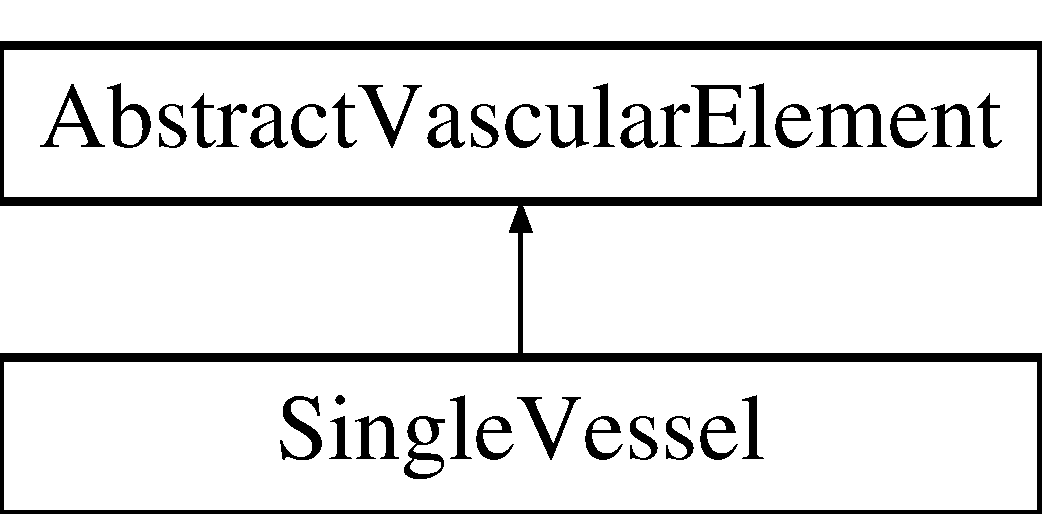
\includegraphics[height=2.000000cm]{da/d40/class_single_vessel}
\end{center}
\end{figure}
\subsection*{Public Member Functions}
\begin{DoxyCompactItemize}
\item 
void \hyperlink{class_single_vessel_a6e397458482fd04bc3c1514eb518f05b}{get\+Branching\+Points} (vector$<$ \hyperlink{structpoint}{point} $>$ $\ast$branching\+Points, \hyperlink{structpoint}{point} x\+New)
\item 
\hyperlink{class_abstract_vascular_element}{Abstract\+Vascular\+Element} $\ast$ \hyperlink{class_single_vessel_a7b905db74d4f733ea3cdb86ec961e9d1}{get\+Parent} ()
\item 
\hyperlink{class_single_vessel}{Single\+Vessel} $\ast$ \hyperlink{class_single_vessel_a25b7df0247aea7a482566de82c56ff3f}{get\+Parent\+Vessel\+To} (\hyperlink{structpoint}{point} xp)
\item 
vector$<$ \hyperlink{class_abstract_vascular_element}{Abstract\+Vascular\+Element} $\ast$ $>$ \& \hyperlink{class_single_vessel_a982d61ce4b6025bc07a4ccc95e1acc9f}{get\+Children} ()
\item 
vector$<$ \hyperlink{class_single_vessel}{Single\+Vessel} $\ast$ $>$ $\ast$ \hyperlink{class_single_vessel_a159e7d2d69cd3cae7b26f2ca374da817}{get\+Children\+Vessel\+To} (\hyperlink{structpoint}{point} xd)
\item 
vector$<$ \hyperlink{class_single_vessel}{Single\+Vessel} $\ast$ $>$ $\ast$ \hyperlink{class_single_vessel_a42b2be50278e2c5ffe63d013b17e9713}{get\+Vessels\+Connected\+To} (\hyperlink{structpoint}{point} p)
\item 
long long int \hyperlink{class_single_vessel_a91a1cfd8cae1063b268cf1794859a245}{get\+Terminals} ()
\item 
long long int {\bfseries get\+Terminals} (\hyperlink{class_abstract_vascular_element_a9c7d6ae9fe8c220ddad143208b0a5a11}{T\+E\+R\+M\+I\+N\+A\+L\+\_\+\+T\+Y\+PE} type)\hypertarget{class_single_vessel_ab9802f20fabbb352c91a3082980e543c}{}\label{class_single_vessel_ab9802f20fabbb352c91a3082980e543c}

\item 
double \hyperlink{class_single_vessel_ac2cb07695080b9c7c6da65a2d52e0a51}{get\+Volume} ()
\item 
void \hyperlink{class_single_vessel_adb7b986bc0da45d0720caf08989e00ce}{update\+Pressure} ()
\item 
double \hyperlink{class_single_vessel_ac50e2a301750d3e6c64fa3e5fc37f79e}{get\+Terminal\+Flow} (double q\+Prox, double q\+Reserved, int common\+Terminals)
\item 
double \hyperlink{class_single_vessel_a934c1d6b9a590621d53d78fedfed4c30}{get\+Distal\+Radius} ()
\item 
double \hyperlink{class_single_vessel_a439762c206fe749024ecc8c601d51738}{get\+Proximal\+Pressure} ()
\item 
void \hyperlink{class_single_vessel_a11c4b9cfc4248dafda09d6a3ab8a60c7}{save\+Vessel\+Data} (ofstream $\ast$tree\+File)
\item 
void \hyperlink{class_single_vessel_a84bfe24d24716e35cc1b811eea2a6ec8}{save\+Vessel\+Connectivity} (ofstream $\ast$tree\+File)
\end{DoxyCompactItemize}
\subsection*{Public Attributes}
\begin{DoxyCompactItemize}
\item 
vtk\+Smart\+Pointer$<$ vtk\+Line $>$ \hyperlink{class_single_vessel_af37e0b95e68662ded08ef7037b64b7e4}{vtk\+Segment}
\item 
vtk\+Id\+Type \hyperlink{class_single_vessel_aa283409729185f57950d58a483b7d661}{vtk\+Segment\+Id}
\item 
\hyperlink{structpoint}{point} \hyperlink{class_single_vessel_a22d0c3617e92838a3a45310b9cbe7f91}{x\+Prox}
\item 
\hyperlink{structpoint}{point} \hyperlink{class_single_vessel_aff9be7494294fb039b2aa284eb39c171}{x\+Dist}
\item 
int \hyperlink{class_single_vessel_acb4f005fc124382aa5dac06194b43007}{n\+Level}
\item 
double \hyperlink{class_single_vessel_a972becbedffb100e3839f5fb06d54ee3}{radius}
\item 
double \hyperlink{class_single_vessel_ae31525b610b4ef7f7c61db0446a983a2}{beta}
\item 
double \hyperlink{class_single_vessel_af96ace62c72b4c495e625724fdc69c1f}{length}
\item 
double \hyperlink{class_single_vessel_ac629f35d34a3adb31f92b06823b320b2}{resistance}
\item 
double \hyperlink{class_single_vessel_a8f5954708c5334dc8ed9f10693381566}{local\+Resistance}
\item 
double \hyperlink{class_single_vessel_ab11b1dc88a1725b79d6ef2344680cf77}{viscosity}
\item 
double \hyperlink{class_single_vessel_a31a369f55958ce8d945fab6781e577c4}{flow}
\item 
double \hyperlink{class_single_vessel_af3e07bf47e7fbc3f04bfa9c7aaa51926}{pressure}
\item 
long long int \hyperlink{class_single_vessel_ab59549ae5a43283077be9bbb25cc01a6}{ID}
\item 
double \hyperlink{class_single_vessel_a2d9634eeadb4fce742f5bfdf4f9077ed}{tree\+Volume}
\end{DoxyCompactItemize}
\subsection*{Static Public Attributes}
\begin{DoxyCompactItemize}
\item 
static int \hyperlink{class_single_vessel_a4ba9764d805e456b1a5a911547bafe87}{bifurcation\+Tests} = 6
\end{DoxyCompactItemize}
\subsection*{Additional Inherited Members}


\subsection{Detailed Description}
Composite vessel structure that for a single rectilinear vessel. 

\subsection{Member Function Documentation}
\index{Single\+Vessel@{Single\+Vessel}!get\+Branching\+Points@{get\+Branching\+Points}}
\index{get\+Branching\+Points@{get\+Branching\+Points}!Single\+Vessel@{Single\+Vessel}}
\subsubsection[{\texorpdfstring{get\+Branching\+Points(vector$<$ point $>$ $\ast$branching\+Points, point x\+New)}{getBranchingPoints(vector< point > *branchingPoints, point xNew)}}]{\setlength{\rightskip}{0pt plus 5cm}void Single\+Vessel\+::get\+Branching\+Points (
\begin{DoxyParamCaption}
\item[{vector$<$ {\bf point} $>$ $\ast$}]{branching\+Points, }
\item[{{\bf point}}]{x\+New}
\end{DoxyParamCaption}
)\hspace{0.3cm}{\ttfamily [virtual]}}\hypertarget{class_single_vessel_a6e397458482fd04bc3c1514eb518f05b}{}\label{class_single_vessel_a6e397458482fd04bc3c1514eb518f05b}
Fill {\ttfamily branching\+Points} with the potential points for branching in the current vessel, accorading to the {\ttfamily branching\+Mode}. 
\begin{DoxyParams}{Parameters}
{\em branching\+Points} & Vector filled with the possible branching points of this vessel. \\
\hline
{\em x\+New} & Terminal position of the new vessel to branch with. \\
\hline
\end{DoxyParams}


Implements \hyperlink{class_abstract_vascular_element_a0ec4dde7ce06f1d977d19b5a340eca52}{Abstract\+Vascular\+Element}.

\index{Single\+Vessel@{Single\+Vessel}!get\+Children@{get\+Children}}
\index{get\+Children@{get\+Children}!Single\+Vessel@{Single\+Vessel}}
\subsubsection[{\texorpdfstring{get\+Children()}{getChildren()}}]{\setlength{\rightskip}{0pt plus 5cm}vector$<$ {\bf Abstract\+Vascular\+Element} $\ast$ $>$ \& Single\+Vessel\+::get\+Children (
\begin{DoxyParamCaption}
{}
\end{DoxyParamCaption}
)\hspace{0.3cm}{\ttfamily [virtual]}}\hypertarget{class_single_vessel_a982d61ce4b6025bc07a4ccc95e1acc9f}{}\label{class_single_vessel_a982d61ce4b6025bc07a4ccc95e1acc9f}
Returns all the children vessels to this vascular element. \begin{DoxyReturn}{Returns}
Children vessels to this vascular element. 
\end{DoxyReturn}


Implements \hyperlink{class_abstract_vascular_element_ae9cf2675f971fa470c74403c8b923f7d}{Abstract\+Vascular\+Element}.

\index{Single\+Vessel@{Single\+Vessel}!get\+Children\+Vessel\+To@{get\+Children\+Vessel\+To}}
\index{get\+Children\+Vessel\+To@{get\+Children\+Vessel\+To}!Single\+Vessel@{Single\+Vessel}}
\subsubsection[{\texorpdfstring{get\+Children\+Vessel\+To(point xd)}{getChildrenVesselTo(point xd)}}]{\setlength{\rightskip}{0pt plus 5cm}vector$<$ {\bf Single\+Vessel} $\ast$ $>$ $\ast$ Single\+Vessel\+::get\+Children\+Vessel\+To (
\begin{DoxyParamCaption}
\item[{{\bf point}}]{xd}
\end{DoxyParamCaption}
)\hspace{0.3cm}{\ttfamily [virtual]}}\hypertarget{class_single_vessel_a159e7d2d69cd3cae7b26f2ca374da817}{}\label{class_single_vessel_a159e7d2d69cd3cae7b26f2ca374da817}
Returns all \hyperlink{class_single_vessel}{Single\+Vessel} that are children of this vascular element. 
\begin{DoxyParams}{Parameters}
{\em xd} & Point of children vessels attachment. \\
\hline
\end{DoxyParams}
\begin{DoxyReturn}{Returns}
\hyperlink{class_single_vessel}{Single\+Vessel} that is parent for this vascular element. 
\end{DoxyReturn}


Implements \hyperlink{class_abstract_vascular_element_aac4f9650c704d920903c49270b18f717}{Abstract\+Vascular\+Element}.

\index{Single\+Vessel@{Single\+Vessel}!get\+Distal\+Radius@{get\+Distal\+Radius}}
\index{get\+Distal\+Radius@{get\+Distal\+Radius}!Single\+Vessel@{Single\+Vessel}}
\subsubsection[{\texorpdfstring{get\+Distal\+Radius()}{getDistalRadius()}}]{\setlength{\rightskip}{0pt plus 5cm}double Single\+Vessel\+::get\+Distal\+Radius (
\begin{DoxyParamCaption}
{}
\end{DoxyParamCaption}
)\hspace{0.3cm}{\ttfamily [virtual]}}\hypertarget{class_single_vessel_a934c1d6b9a590621d53d78fedfed4c30}{}\label{class_single_vessel_a934c1d6b9a590621d53d78fedfed4c30}
Returns the radius at the distal point of the vessel. \begin{DoxyReturn}{Returns}
Radius at the distal point of the vessel. 
\end{DoxyReturn}


Implements \hyperlink{class_abstract_vascular_element_a3880bed8d0a9223107bcee195bb89e51}{Abstract\+Vascular\+Element}.

\index{Single\+Vessel@{Single\+Vessel}!get\+Parent@{get\+Parent}}
\index{get\+Parent@{get\+Parent}!Single\+Vessel@{Single\+Vessel}}
\subsubsection[{\texorpdfstring{get\+Parent()}{getParent()}}]{\setlength{\rightskip}{0pt plus 5cm}{\bf Abstract\+Vascular\+Element} $\ast$ Single\+Vessel\+::get\+Parent (
\begin{DoxyParamCaption}
{}
\end{DoxyParamCaption}
)\hspace{0.3cm}{\ttfamily [virtual]}}\hypertarget{class_single_vessel_a7b905db74d4f733ea3cdb86ec961e9d1}{}\label{class_single_vessel_a7b905db74d4f733ea3cdb86ec961e9d1}
Returns its parental \hyperlink{class_abstract_vascular_element}{Abstract\+Vascular\+Element}. \begin{DoxyReturn}{Returns}
\hyperlink{class_abstract_vascular_element}{Abstract\+Vascular\+Element} proximally attached. 
\end{DoxyReturn}


Implements \hyperlink{class_abstract_vascular_element_aab59dfe7c6d4c846cb8f341727be8261}{Abstract\+Vascular\+Element}.

\index{Single\+Vessel@{Single\+Vessel}!get\+Parent\+Vessel\+To@{get\+Parent\+Vessel\+To}}
\index{get\+Parent\+Vessel\+To@{get\+Parent\+Vessel\+To}!Single\+Vessel@{Single\+Vessel}}
\subsubsection[{\texorpdfstring{get\+Parent\+Vessel\+To(point xp)}{getParentVesselTo(point xp)}}]{\setlength{\rightskip}{0pt plus 5cm}{\bf Single\+Vessel} $\ast$ Single\+Vessel\+::get\+Parent\+Vessel\+To (
\begin{DoxyParamCaption}
\item[{{\bf point}}]{xp}
\end{DoxyParamCaption}
)\hspace{0.3cm}{\ttfamily [virtual]}}\hypertarget{class_single_vessel_a25b7df0247aea7a482566de82c56ff3f}{}\label{class_single_vessel_a25b7df0247aea7a482566de82c56ff3f}
Returns the \hyperlink{class_single_vessel}{Single\+Vessel} that is parent for this vascular element. 
\begin{DoxyParams}{Parameters}
{\em xp} & Point of parent vessel attachment. \\
\hline
\end{DoxyParams}
\begin{DoxyReturn}{Returns}
\hyperlink{class_single_vessel}{Single\+Vessel} that is parent for this vascular element. 
\end{DoxyReturn}


Implements \hyperlink{class_abstract_vascular_element_a4007ab14544d8fb5cacf5c610e9b0e5d}{Abstract\+Vascular\+Element}.

\index{Single\+Vessel@{Single\+Vessel}!get\+Proximal\+Pressure@{get\+Proximal\+Pressure}}
\index{get\+Proximal\+Pressure@{get\+Proximal\+Pressure}!Single\+Vessel@{Single\+Vessel}}
\subsubsection[{\texorpdfstring{get\+Proximal\+Pressure()}{getProximalPressure()}}]{\setlength{\rightskip}{0pt plus 5cm}double Single\+Vessel\+::get\+Proximal\+Pressure (
\begin{DoxyParamCaption}
{}
\end{DoxyParamCaption}
)\hspace{0.3cm}{\ttfamily [virtual]}}\hypertarget{class_single_vessel_a439762c206fe749024ecc8c601d51738}{}\label{class_single_vessel_a439762c206fe749024ecc8c601d51738}
Returns the pressure at the proximal point of the vessel. \begin{DoxyReturn}{Returns}
Pressure at the proximal point of the vessel. 
\end{DoxyReturn}


Implements \hyperlink{class_abstract_vascular_element_aa486370af563a9ea9bfcdcde8ee38426}{Abstract\+Vascular\+Element}.

\index{Single\+Vessel@{Single\+Vessel}!get\+Terminal\+Flow@{get\+Terminal\+Flow}}
\index{get\+Terminal\+Flow@{get\+Terminal\+Flow}!Single\+Vessel@{Single\+Vessel}}
\subsubsection[{\texorpdfstring{get\+Terminal\+Flow(double q\+Prox, double q\+Reserved, int common\+Terminals)}{getTerminalFlow(double qProx, double qReserved, int commonTerminals)}}]{\setlength{\rightskip}{0pt plus 5cm}double Single\+Vessel\+::get\+Terminal\+Flow (
\begin{DoxyParamCaption}
\item[{double}]{q\+Prox, }
\item[{double}]{q\+Reserved, }
\item[{int}]{common\+Terminals}
\end{DoxyParamCaption}
)}\hypertarget{class_single_vessel_ac50e2a301750d3e6c64fa3e5fc37f79e}{}\label{class_single_vessel_ac50e2a301750d3e6c64fa3e5fc37f79e}
Determine the flow at this terminal based on tree information (e.\+g. amount of terminals and inflow). 
\begin{DoxyParams}{Parameters}
{\em tree} & Tree that contains this vessel. \\
\hline
\end{DoxyParams}
\begin{DoxyReturn}{Returns}
Amount of flow outgoing this terminal. 
\end{DoxyReturn}
\index{Single\+Vessel@{Single\+Vessel}!get\+Terminals@{get\+Terminals}}
\index{get\+Terminals@{get\+Terminals}!Single\+Vessel@{Single\+Vessel}}
\subsubsection[{\texorpdfstring{get\+Terminals()}{getTerminals()}}]{\setlength{\rightskip}{0pt plus 5cm}long long int Single\+Vessel\+::get\+Terminals (
\begin{DoxyParamCaption}
{}
\end{DoxyParamCaption}
)\hspace{0.3cm}{\ttfamily [virtual]}}\hypertarget{class_single_vessel_a91a1cfd8cae1063b268cf1794859a245}{}\label{class_single_vessel_a91a1cfd8cae1063b268cf1794859a245}
Returns all the inner terminals in the current vascular element. \begin{DoxyReturn}{Returns}
Terminals in the current vascular element. 
\end{DoxyReturn}


Implements \hyperlink{class_abstract_vascular_element_a85d8d19d6f92a4e7cc95cc0f8f5a59c9}{Abstract\+Vascular\+Element}.

\index{Single\+Vessel@{Single\+Vessel}!get\+Vessels\+Connected\+To@{get\+Vessels\+Connected\+To}}
\index{get\+Vessels\+Connected\+To@{get\+Vessels\+Connected\+To}!Single\+Vessel@{Single\+Vessel}}
\subsubsection[{\texorpdfstring{get\+Vessels\+Connected\+To(point p)}{getVesselsConnectedTo(point p)}}]{\setlength{\rightskip}{0pt plus 5cm}vector$<$ {\bf Single\+Vessel} $\ast$ $>$ $\ast$ Single\+Vessel\+::get\+Vessels\+Connected\+To (
\begin{DoxyParamCaption}
\item[{{\bf point}}]{p}
\end{DoxyParamCaption}
)\hspace{0.3cm}{\ttfamily [virtual]}}\hypertarget{class_single_vessel_a42b2be50278e2c5ffe63d013b17e9713}{}\label{class_single_vessel_a42b2be50278e2c5ffe63d013b17e9713}
Returns all vessels in this vascular structure connected to point {\ttfamily p}. 
\begin{DoxyParams}{Parameters}
{\em p} & Point at which all target vessels are connected to. \\
\hline
\end{DoxyParams}
\begin{DoxyReturn}{Returns}
Set of vessels connected to {\ttfamily p}. 
\end{DoxyReturn}


Implements \hyperlink{class_abstract_vascular_element_a7720067153a223d373c26e14155553e3}{Abstract\+Vascular\+Element}.

\index{Single\+Vessel@{Single\+Vessel}!get\+Volume@{get\+Volume}}
\index{get\+Volume@{get\+Volume}!Single\+Vessel@{Single\+Vessel}}
\subsubsection[{\texorpdfstring{get\+Volume()}{getVolume()}}]{\setlength{\rightskip}{0pt plus 5cm}double Single\+Vessel\+::get\+Volume (
\begin{DoxyParamCaption}
{}
\end{DoxyParamCaption}
)\hspace{0.3cm}{\ttfamily [virtual]}}\hypertarget{class_single_vessel_ac2cb07695080b9c7c6da65a2d52e0a51}{}\label{class_single_vessel_ac2cb07695080b9c7c6da65a2d52e0a51}
Returns the functional cost contribution of this vascular element. If any constraint --e.\+g. geometric constrains-- are violated the function must return I\+N\+F\+I\+N\+I\+TY. \begin{DoxyReturn}{Returns}
Functional cost contribution. 
\end{DoxyReturn}


Implements \hyperlink{class_abstract_vascular_element_ae4ecb632a94e89ac21f6523637bdb9cd}{Abstract\+Vascular\+Element}.

\index{Single\+Vessel@{Single\+Vessel}!save\+Vessel\+Connectivity@{save\+Vessel\+Connectivity}}
\index{save\+Vessel\+Connectivity@{save\+Vessel\+Connectivity}!Single\+Vessel@{Single\+Vessel}}
\subsubsection[{\texorpdfstring{save\+Vessel\+Connectivity(ofstream $\ast$tree\+File)}{saveVesselConnectivity(ofstream *treeFile)}}]{\setlength{\rightskip}{0pt plus 5cm}void Single\+Vessel\+::save\+Vessel\+Connectivity (
\begin{DoxyParamCaption}
\item[{ofstream $\ast$}]{tree\+File}
\end{DoxyParamCaption}
)\hspace{0.3cm}{\ttfamily [virtual]}}\hypertarget{class_single_vessel_a84bfe24d24716e35cc1b811eea2a6ec8}{}\label{class_single_vessel_a84bfe24d24716e35cc1b811eea2a6ec8}
Writes connectivity of this vessel at the file associated to {\ttfamily tree\+File} stream. 
\begin{DoxyParams}{Parameters}
{\em tree\+File} & Output file stream. \\
\hline
\end{DoxyParams}


Implements \hyperlink{class_abstract_vascular_element_a878c2826beb1a549c28659182760fbab}{Abstract\+Vascular\+Element}.

\index{Single\+Vessel@{Single\+Vessel}!save\+Vessel\+Data@{save\+Vessel\+Data}}
\index{save\+Vessel\+Data@{save\+Vessel\+Data}!Single\+Vessel@{Single\+Vessel}}
\subsubsection[{\texorpdfstring{save\+Vessel\+Data(ofstream $\ast$tree\+File)}{saveVesselData(ofstream *treeFile)}}]{\setlength{\rightskip}{0pt plus 5cm}void Single\+Vessel\+::save\+Vessel\+Data (
\begin{DoxyParamCaption}
\item[{ofstream $\ast$}]{tree\+File}
\end{DoxyParamCaption}
)\hspace{0.3cm}{\ttfamily [virtual]}}\hypertarget{class_single_vessel_a11c4b9cfc4248dafda09d6a3ab8a60c7}{}\label{class_single_vessel_a11c4b9cfc4248dafda09d6a3ab8a60c7}
Writes the vessel data at the file associated to {\ttfamily tree\+File} stream. 
\begin{DoxyParams}{Parameters}
{\em tree\+File} & Output file stream. \\
\hline
\end{DoxyParams}


Implements \hyperlink{class_abstract_vascular_element_aff5f129b31f0c82aebf2d7387859914d}{Abstract\+Vascular\+Element}.

\index{Single\+Vessel@{Single\+Vessel}!update\+Pressure@{update\+Pressure}}
\index{update\+Pressure@{update\+Pressure}!Single\+Vessel@{Single\+Vessel}}
\subsubsection[{\texorpdfstring{update\+Pressure()}{updatePressure()}}]{\setlength{\rightskip}{0pt plus 5cm}void Single\+Vessel\+::update\+Pressure (
\begin{DoxyParamCaption}
{}
\end{DoxyParamCaption}
)\hspace{0.3cm}{\ttfamily [virtual]}}\hypertarget{class_single_vessel_adb7b986bc0da45d0720caf08989e00ce}{}\label{class_single_vessel_adb7b986bc0da45d0720caf08989e00ce}
Updates vascular element pressure from children to parent direction. 

Implements \hyperlink{class_abstract_vascular_element_a258a830359614d0217e820293a9bdaa9}{Abstract\+Vascular\+Element}.



\subsection{Member Data Documentation}
\index{Single\+Vessel@{Single\+Vessel}!beta@{beta}}
\index{beta@{beta}!Single\+Vessel@{Single\+Vessel}}
\subsubsection[{\texorpdfstring{beta}{beta}}]{\setlength{\rightskip}{0pt plus 5cm}double Single\+Vessel\+::beta}\hypertarget{class_single_vessel_ae31525b610b4ef7f7c61db0446a983a2}{}\label{class_single_vessel_ae31525b610b4ef7f7c61db0446a983a2}
Radius relative to the parent vessel (i.\+e. radius/parent\+\_\+radius). For root, it is the radius value. \index{Single\+Vessel@{Single\+Vessel}!bifurcation\+Tests@{bifurcation\+Tests}}
\index{bifurcation\+Tests@{bifurcation\+Tests}!Single\+Vessel@{Single\+Vessel}}
\subsubsection[{\texorpdfstring{bifurcation\+Tests}{bifurcationTests}}]{\setlength{\rightskip}{0pt plus 5cm}int Single\+Vessel\+::bifurcation\+Tests = 6\hspace{0.3cm}{\ttfamily [static]}}\hypertarget{class_single_vessel_a4ba9764d805e456b1a5a911547bafe87}{}\label{class_single_vessel_a4ba9764d805e456b1a5a911547bafe87}
Points to be tested for branching in D\+E\+F\+O\+R\+M\+A\+B\+L\+E\+\_\+\+P\+A\+R\+E\+NT mode. \index{Single\+Vessel@{Single\+Vessel}!flow@{flow}}
\index{flow@{flow}!Single\+Vessel@{Single\+Vessel}}
\subsubsection[{\texorpdfstring{flow}{flow}}]{\setlength{\rightskip}{0pt plus 5cm}double Single\+Vessel\+::flow}\hypertarget{class_single_vessel_a31a369f55958ce8d945fab6781e577c4}{}\label{class_single_vessel_a31a369f55958ce8d945fab6781e577c4}
Flow in this vessel. \index{Single\+Vessel@{Single\+Vessel}!ID@{ID}}
\index{ID@{ID}!Single\+Vessel@{Single\+Vessel}}
\subsubsection[{\texorpdfstring{ID}{ID}}]{\setlength{\rightskip}{0pt plus 5cm}long long int Single\+Vessel\+::\+ID}\hypertarget{class_single_vessel_ab59549ae5a43283077be9bbb25cc01a6}{}\label{class_single_vessel_ab59549ae5a43283077be9bbb25cc01a6}
Generation step \index{Single\+Vessel@{Single\+Vessel}!length@{length}}
\index{length@{length}!Single\+Vessel@{Single\+Vessel}}
\subsubsection[{\texorpdfstring{length}{length}}]{\setlength{\rightskip}{0pt plus 5cm}double Single\+Vessel\+::length}\hypertarget{class_single_vessel_af96ace62c72b4c495e625724fdc69c1f}{}\label{class_single_vessel_af96ace62c72b4c495e625724fdc69c1f}
Distance between x\+Prox and x\+Dist. \index{Single\+Vessel@{Single\+Vessel}!local\+Resistance@{local\+Resistance}}
\index{local\+Resistance@{local\+Resistance}!Single\+Vessel@{Single\+Vessel}}
\subsubsection[{\texorpdfstring{local\+Resistance}{localResistance}}]{\setlength{\rightskip}{0pt plus 5cm}double Single\+Vessel\+::local\+Resistance}\hypertarget{class_single_vessel_a8f5954708c5334dc8ed9f10693381566}{}\label{class_single_vessel_a8f5954708c5334dc8ed9f10693381566}
Local fluid-\/dynamic resistance. \index{Single\+Vessel@{Single\+Vessel}!n\+Level@{n\+Level}}
\index{n\+Level@{n\+Level}!Single\+Vessel@{Single\+Vessel}}
\subsubsection[{\texorpdfstring{n\+Level}{nLevel}}]{\setlength{\rightskip}{0pt plus 5cm}int Single\+Vessel\+::n\+Level}\hypertarget{class_single_vessel_acb4f005fc124382aa5dac06194b43007}{}\label{class_single_vessel_acb4f005fc124382aa5dac06194b43007}
Bifurcation level from proximal to distal (Root is at level 0). \index{Single\+Vessel@{Single\+Vessel}!pressure@{pressure}}
\index{pressure@{pressure}!Single\+Vessel@{Single\+Vessel}}
\subsubsection[{\texorpdfstring{pressure}{pressure}}]{\setlength{\rightskip}{0pt plus 5cm}double Single\+Vessel\+::pressure}\hypertarget{class_single_vessel_af3e07bf47e7fbc3f04bfa9c7aaa51926}{}\label{class_single_vessel_af3e07bf47e7fbc3f04bfa9c7aaa51926}
Pressure in the vessel. \index{Single\+Vessel@{Single\+Vessel}!radius@{radius}}
\index{radius@{radius}!Single\+Vessel@{Single\+Vessel}}
\subsubsection[{\texorpdfstring{radius}{radius}}]{\setlength{\rightskip}{0pt plus 5cm}double Single\+Vessel\+::radius}\hypertarget{class_single_vessel_a972becbedffb100e3839f5fb06d54ee3}{}\label{class_single_vessel_a972becbedffb100e3839f5fb06d54ee3}
Vessel radius. \index{Single\+Vessel@{Single\+Vessel}!resistance@{resistance}}
\index{resistance@{resistance}!Single\+Vessel@{Single\+Vessel}}
\subsubsection[{\texorpdfstring{resistance}{resistance}}]{\setlength{\rightskip}{0pt plus 5cm}double Single\+Vessel\+::resistance}\hypertarget{class_single_vessel_ac629f35d34a3adb31f92b06823b320b2}{}\label{class_single_vessel_ac629f35d34a3adb31f92b06823b320b2}
Reduced fluid-\/dynamic resistance. \index{Single\+Vessel@{Single\+Vessel}!tree\+Volume@{tree\+Volume}}
\index{tree\+Volume@{tree\+Volume}!Single\+Vessel@{Single\+Vessel}}
\subsubsection[{\texorpdfstring{tree\+Volume}{treeVolume}}]{\setlength{\rightskip}{0pt plus 5cm}double Single\+Vessel\+::tree\+Volume}\hypertarget{class_single_vessel_a2d9634eeadb4fce742f5bfdf4f9077ed}{}\label{class_single_vessel_a2d9634eeadb4fce742f5bfdf4f9077ed}
Volume of this down tree branch. \index{Single\+Vessel@{Single\+Vessel}!viscosity@{viscosity}}
\index{viscosity@{viscosity}!Single\+Vessel@{Single\+Vessel}}
\subsubsection[{\texorpdfstring{viscosity}{viscosity}}]{\setlength{\rightskip}{0pt plus 5cm}double Single\+Vessel\+::viscosity}\hypertarget{class_single_vessel_ab11b1dc88a1725b79d6ef2344680cf77}{}\label{class_single_vessel_ab11b1dc88a1725b79d6ef2344680cf77}
Blood viscosity. \index{Single\+Vessel@{Single\+Vessel}!vtk\+Segment@{vtk\+Segment}}
\index{vtk\+Segment@{vtk\+Segment}!Single\+Vessel@{Single\+Vessel}}
\subsubsection[{\texorpdfstring{vtk\+Segment}{vtkSegment}}]{\setlength{\rightskip}{0pt plus 5cm}vtk\+Smart\+Pointer$<$vtk\+Line$>$ Single\+Vessel\+::vtk\+Segment}\hypertarget{class_single_vessel_af37e0b95e68662ded08ef7037b64b7e4}{}\label{class_single_vessel_af37e0b95e68662ded08ef7037b64b7e4}
V\+TK geomtric representation. \index{Single\+Vessel@{Single\+Vessel}!vtk\+Segment\+Id@{vtk\+Segment\+Id}}
\index{vtk\+Segment\+Id@{vtk\+Segment\+Id}!Single\+Vessel@{Single\+Vessel}}
\subsubsection[{\texorpdfstring{vtk\+Segment\+Id}{vtkSegmentId}}]{\setlength{\rightskip}{0pt plus 5cm}vtk\+Id\+Type Single\+Vessel\+::vtk\+Segment\+Id}\hypertarget{class_single_vessel_aa283409729185f57950d58a483b7d661}{}\label{class_single_vessel_aa283409729185f57950d58a483b7d661}
Unique identifier for the vessel. \index{Single\+Vessel@{Single\+Vessel}!x\+Dist@{x\+Dist}}
\index{x\+Dist@{x\+Dist}!Single\+Vessel@{Single\+Vessel}}
\subsubsection[{\texorpdfstring{x\+Dist}{xDist}}]{\setlength{\rightskip}{0pt plus 5cm}{\bf point} Single\+Vessel\+::x\+Dist}\hypertarget{class_single_vessel_aff9be7494294fb039b2aa284eb39c171}{}\label{class_single_vessel_aff9be7494294fb039b2aa284eb39c171}
Distal position of the vessel. \index{Single\+Vessel@{Single\+Vessel}!x\+Prox@{x\+Prox}}
\index{x\+Prox@{x\+Prox}!Single\+Vessel@{Single\+Vessel}}
\subsubsection[{\texorpdfstring{x\+Prox}{xProx}}]{\setlength{\rightskip}{0pt plus 5cm}{\bf point} Single\+Vessel\+::x\+Prox}\hypertarget{class_single_vessel_a22d0c3617e92838a3a45310b9cbe7f91}{}\label{class_single_vessel_a22d0c3617e92838a3a45310b9cbe7f91}
Proximal position of the vessel. 

The documentation for this class was generated from the following files\+:\begin{DoxyCompactItemize}
\item 
structures/vascular\+Elements/Single\+Vessel.\+h\item 
structures/vascular\+Elements/Single\+Vessel.\+cpp\end{DoxyCompactItemize}

\hypertarget{class_single_vessel_c_c_o_o_tree}{}\section{Single\+Vessel\+C\+C\+O\+O\+Tree Class Reference}
\label{class_single_vessel_c_c_o_o_tree}\index{Single\+Vessel\+C\+C\+O\+O\+Tree@{Single\+Vessel\+C\+C\+O\+O\+Tree}}


{\ttfamily \#include $<$Single\+Vessel\+C\+C\+O\+O\+Tree.\+h$>$}

Inheritance diagram for Single\+Vessel\+C\+C\+O\+O\+Tree\+:\begin{figure}[H]
\begin{center}
\leavevmode
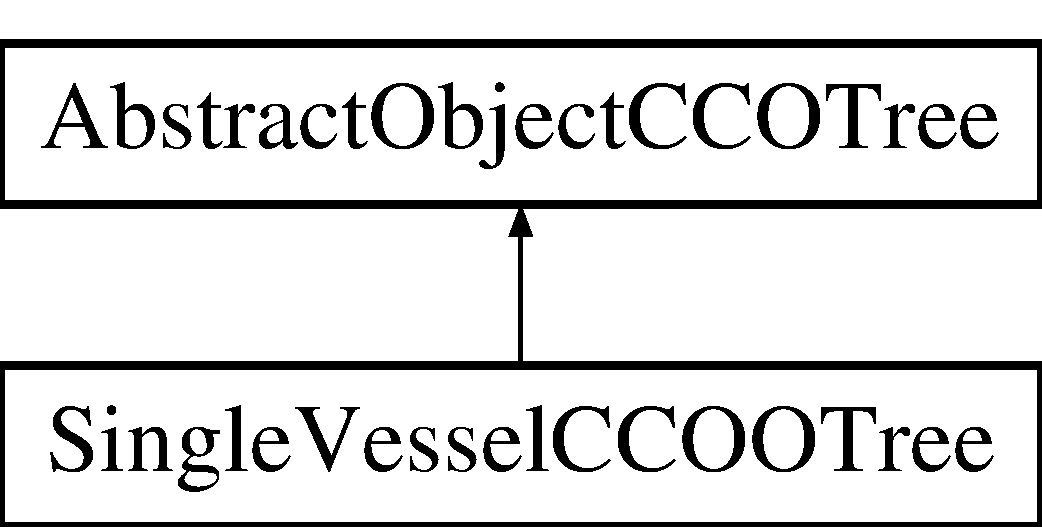
\includegraphics[height=2.000000cm]{dc/d93/class_single_vessel_c_c_o_o_tree}
\end{center}
\end{figure}
\subsection*{Public Member Functions}
\begin{DoxyCompactItemize}
\item 
\hyperlink{class_single_vessel_c_c_o_o_tree_a0151dcbe49ac8b9e792930d702afe890}{Single\+Vessel\+C\+C\+O\+O\+Tree} (\hyperlink{structpoint}{point} xi, double \hyperlink{class_single_vessel_c_c_o_o_tree_a92984c132be3e2eaed34adfc261afa48}{root\+Radius}, double qi, \hyperlink{class_abstract_constraint_function}{Abstract\+Constraint\+Function}$<$ double, int $>$ $\ast$\hyperlink{class_abstract_object_c_c_o_tree_aad315b93744637e18153c4434dac067d}{gam}, \hyperlink{class_abstract_constraint_function}{Abstract\+Constraint\+Function}$<$ double, int $>$ $\ast$\hyperlink{class_abstract_object_c_c_o_tree_a62d3e1ff7e74a6236422273f58fc6012}{eps\+Lim}, \hyperlink{class_abstract_constraint_function}{Abstract\+Constraint\+Function}$<$ double, int $>$ $\ast$\hyperlink{class_abstract_object_c_c_o_tree_a92e6b6d1a2fac7331eee34fb28158828}{nu}, double \hyperlink{class_abstract_object_c_c_o_tree_ae7215e6237e4d04625a0c96be9f3578d}{ref\+Pressure}, double resistance\+Variation\+Tolerance, \hyperlink{class_generator_data}{Generator\+Data} $\ast$\hyperlink{class_abstract_object_c_c_o_tree_aca7aecbd89dadc46dd9dce14cfde31e1}{instance\+Data})
\item 
\hyperlink{class_single_vessel_c_c_o_o_tree_ae26fe0d30497926f2ea0f043d4d19804}{Single\+Vessel\+C\+C\+O\+O\+Tree} (string filename\+C\+CO, \hyperlink{class_generator_data}{Generator\+Data} $\ast$\hyperlink{class_abstract_object_c_c_o_tree_aca7aecbd89dadc46dd9dce14cfde31e1}{instance\+Data}, \hyperlink{class_abstract_constraint_function}{Abstract\+Constraint\+Function}$<$ double, int $>$ $\ast$\hyperlink{class_abstract_object_c_c_o_tree_aad315b93744637e18153c4434dac067d}{gam}, \hyperlink{class_abstract_constraint_function}{Abstract\+Constraint\+Function}$<$ double, int $>$ $\ast$\hyperlink{class_abstract_object_c_c_o_tree_a62d3e1ff7e74a6236422273f58fc6012}{eps\+Lim}, \hyperlink{class_abstract_constraint_function}{Abstract\+Constraint\+Function}$<$ double, int $>$ $\ast$\hyperlink{class_abstract_object_c_c_o_tree_a92e6b6d1a2fac7331eee34fb28158828}{nu})
\item 
\hyperlink{class_single_vessel_c_c_o_o_tree_a3b95648509148c82901f8f930ed06b1c}{Single\+Vessel\+C\+C\+O\+O\+Tree} (string filename\+C\+CO, \hyperlink{class_generator_data}{Generator\+Data} $\ast$\hyperlink{class_abstract_object_c_c_o_tree_aca7aecbd89dadc46dd9dce14cfde31e1}{instance\+Data}, double qi, \hyperlink{class_abstract_constraint_function}{Abstract\+Constraint\+Function}$<$ double, int $>$ $\ast$\hyperlink{class_abstract_object_c_c_o_tree_aad315b93744637e18153c4434dac067d}{gam}, \hyperlink{class_abstract_constraint_function}{Abstract\+Constraint\+Function}$<$ double, int $>$ $\ast$\hyperlink{class_abstract_object_c_c_o_tree_a62d3e1ff7e74a6236422273f58fc6012}{eps\+Lim}, \hyperlink{class_abstract_constraint_function}{Abstract\+Constraint\+Function}$<$ double, int $>$ $\ast$\hyperlink{class_abstract_object_c_c_o_tree_a92e6b6d1a2fac7331eee34fb28158828}{nu}, double \hyperlink{class_abstract_object_c_c_o_tree_ae7215e6237e4d04625a0c96be9f3578d}{ref\+Pressure}, double viscosity\+Tolerance)
\item 
\hyperlink{class_single_vessel_c_c_o_o_tree_a1c137ac564fb37adef0830032e68e0e0}{$\sim$\+Single\+Vessel\+C\+C\+O\+O\+Tree} ()
\item 
\hyperlink{class_single_vessel_c_c_o_o_tree}{Single\+Vessel\+C\+C\+O\+O\+Tree} $\ast$ \hyperlink{class_single_vessel_c_c_o_o_tree_acff17f1c7f1c69539d94f86e0ffbe267}{clone} ()
\item 
void \hyperlink{class_single_vessel_c_c_o_o_tree_aac665cdb3fa0687f579ef844ac47c5a7}{get\+Closest\+Tree\+Point} (\hyperlink{structpoint}{point} x\+New, \hyperlink{structpoint}{point} $\ast$x\+Bif, double $\ast$dist)
\item 
vector$<$ \hyperlink{class_abstract_vascular_element}{Abstract\+Vascular\+Element} $\ast$ $>$ \hyperlink{class_single_vessel_c_c_o_o_tree_a2c33f20925efececc655c7b8d89c93ed}{get\+Close\+Segments} (\hyperlink{structpoint}{point} x\+New, \hyperlink{class_abstract_domain}{Abstract\+Domain} $\ast$domain, int $\ast$n\+Found)
\item 
void \hyperlink{class_single_vessel_c_c_o_o_tree_ae9f08ba67c5a9a13b17313c9e86ccaa8}{add\+Vessel} (\hyperlink{structpoint}{point} x\+Prox, \hyperlink{structpoint}{point} x\+Dist, \hyperlink{class_abstract_vascular_element}{Abstract\+Vascular\+Element} $\ast$parent, \hyperlink{class_abstract_vascular_element_a7d7b7863aae4952ba79a590ee65702ec}{Abstract\+Vascular\+Element\+::\+V\+E\+S\+S\+E\+L\+\_\+\+F\+U\+N\+C\+T\+I\+ON} vessel\+Function)
\item 
int \hyperlink{class_single_vessel_c_c_o_o_tree_a4efc4561ed2de4d186b16d5b3c006fc2}{test\+Vessel} (\hyperlink{structpoint}{point} x\+New, \hyperlink{class_abstract_vascular_element}{Abstract\+Vascular\+Element} $\ast$parent, \hyperlink{class_abstract_domain}{Abstract\+Domain} $\ast$domain, vector$<$ \hyperlink{class_abstract_vascular_element}{Abstract\+Vascular\+Element} $\ast$ $>$ neighbors, double dlim, \hyperlink{structpoint}{point} $\ast$x\+Bif, double $\ast$cost)
\item 
void \hyperlink{class_single_vessel_c_c_o_o_tree_acc5c5d57cad07202170ecca7f65978cf}{print} ()
\item 
string \hyperlink{class_single_vessel_c_c_o_o_tree_a6aeccd994eeaa106d0c269313d7cf3dc}{get\+Tree\+Name} ()
\item 
double \hyperlink{class_single_vessel_c_c_o_o_tree_a2736be9eef11a5b1e8f45218a8933d84}{get\+Root\+Radius} ()
\item 
void \hyperlink{class_single_vessel_c_c_o_o_tree_a0a3ffdee4f53e21209a187b9539f41ec}{remove\+Withered\+Branches} (int stage)
\item 
void \hyperlink{class_single_vessel_c_c_o_o_tree_a8f8c3457c301d6d8f91ac4ff1a5c2de5}{remove} (\hyperlink{class_single_vessel}{Single\+Vessel} $\ast$\hyperlink{structvessel}{vessel})
\item 
bool \hyperlink{class_single_vessel_c_c_o_o_tree_a9e1b432708271e41cd9a3438d2f2fe44}{is\+Withered} (\hyperlink{class_single_vessel}{Single\+Vessel} $\ast$\hyperlink{structvessel}{vessel})
\end{DoxyCompactItemize}
\subsection*{Protected Member Functions}
\begin{DoxyCompactItemize}
\item 
void \hyperlink{class_single_vessel_c_c_o_o_tree_a4f5ae33e49f3d7ba07e1f4a31ff3568e}{save\+Tree} (ofstream $\ast$out\+File)
\end{DoxyCompactItemize}
\subsection*{Private Member Functions}
\begin{DoxyCompactItemize}
\item 
\hyperlink{class_single_vessel_c_c_o_o_tree}{Single\+Vessel\+C\+C\+O\+O\+Tree} $\ast$ \hyperlink{class_single_vessel_c_c_o_o_tree_afcabe5e4cb15ffdb18097c28ecc72e44}{clone\+Up\+To} (int levels, \hyperlink{class_single_vessel}{Single\+Vessel} $\ast$parent)
\item 
\hyperlink{class_single_vessel}{Single\+Vessel} $\ast$ \hyperlink{class_single_vessel_c_c_o_o_tree_a8fc66762911652eec13b986a69b60e08}{clone\+Tree} (\hyperlink{class_single_vessel}{Single\+Vessel} $\ast$\hyperlink{class_abstract_object_c_c_o_tree_ae1b17938ad34d92629915159c49bb89a}{root}, unordered\+\_\+map$<$ long long, \hyperlink{class_abstract_vascular_element}{Abstract\+Vascular\+Element} $\ast$ $>$ $\ast$segments)
\item 
double \hyperlink{class_single_vessel_c_c_o_o_tree_ac0580b83043a18855988071a2a3f4913}{evaluate} (\hyperlink{structpoint}{point} x\+New, \hyperlink{structpoint}{point} x\+Test, \hyperlink{class_single_vessel}{Single\+Vessel} $\ast$parent, double d\+Lim)
\item 
double \hyperlink{class_single_vessel_c_c_o_o_tree_a154064bf9792abee19671f39c851eb25}{evaluate} (\hyperlink{structpoint}{point} x\+New, \hyperlink{class_single_vessel}{Single\+Vessel} $\ast$parent, double d\+Lim)
\item 
void \hyperlink{class_single_vessel_c_c_o_o_tree_ac8d4ca178e13ed388ad5fe0411ca0b75}{update\+Tree} (\hyperlink{class_single_vessel}{Single\+Vessel} $\ast$\hyperlink{class_abstract_object_c_c_o_tree_ae1b17938ad34d92629915159c49bb89a}{root}, \hyperlink{class_single_vessel_c_c_o_o_tree}{Single\+Vessel\+C\+C\+O\+O\+Tree} $\ast$tree)
\item 
int \hyperlink{class_single_vessel_c_c_o_o_tree_a83661a533a356d3631696b32dee89632}{is\+Symmetrically\+Valid} (double beta1, double beta2, int n\+Level)
\item 
int \hyperlink{class_single_vessel_c_c_o_o_tree_aaf5664ee98d5c6b4b4c0c01a9921a80d}{are\+Valid\+Angles} (\hyperlink{structpoint}{point} x\+Bif, \hyperlink{structpoint}{point} x\+New, \hyperlink{class_single_vessel}{Single\+Vessel} $\ast$parent, double min\+Angle)
\item 
int \hyperlink{class_single_vessel_c_c_o_o_tree_a6c97600f94db54a0df9146880dd601ee}{is\+Valid\+Opening\+Angle} (\hyperlink{structpoint}{point} x\+Bif, \hyperlink{structpoint}{point} x\+New, \hyperlink{class_single_vessel}{Single\+Vessel} $\ast$parent, double min\+Plane\+Angle)
\item 
int \hyperlink{class_single_vessel_c_c_o_o_tree_a7ac08a2e8d1b05eea1d6debf109caaf1}{is\+Intersecting\+Vessels} (\hyperlink{structpoint}{point} p1, \hyperlink{structpoint}{point} p2, \hyperlink{class_single_vessel}{Single\+Vessel} $\ast$parent, vector$<$ \hyperlink{class_abstract_vascular_element}{Abstract\+Vascular\+Element} $\ast$ $>$ neighbors)
\item 
void \hyperlink{class_single_vessel_c_c_o_o_tree_a08fc003426f3a8697af2f57d03a702c9}{update\+Tree\+Viscosities\+Beta} (\hyperlink{class_single_vessel}{Single\+Vessel} $\ast$\hyperlink{class_abstract_object_c_c_o_tree_ae1b17938ad34d92629915159c49bb89a}{root}, double $\ast$max\+Beta\+Variation)
\item 
double \hyperlink{class_single_vessel_c_c_o_o_tree_a125eba238125b220cb021829603e6e97}{get\+Nu\+FL} (double radius)
\item 
void \hyperlink{class_single_vessel_c_c_o_o_tree_ac213538ea943f22310f6c20e47a72170}{create\+Segment\+Vtk\+Lines} (\hyperlink{class_abstract_vascular_element}{Abstract\+Vascular\+Element} $\ast$root\+Vessel)
\end{DoxyCompactItemize}
\subsection*{Private Attributes}
\begin{DoxyCompactItemize}
\item 
double \hyperlink{class_single_vessel_c_c_o_o_tree_a92984c132be3e2eaed34adfc261afa48}{root\+Radius}
\item 
double \hyperlink{class_single_vessel_c_c_o_o_tree_abd14cc5350019a67cc3f8ff881af58e4}{variation\+Tolerance}
\item 
long long int \hyperlink{class_single_vessel_c_c_o_o_tree_a9766e247e4414d77c9a50ed4d09b3138}{n\+Common\+Terminals}
\end{DoxyCompactItemize}
\subsection*{Additional Inherited Members}


\subsection{Detailed Description}
N-\/furcation tree with only \hyperlink{class_single_vessel}{Single\+Vessel} elements as vascular elements. 

\subsection{Constructor \& Destructor Documentation}
\index{Single\+Vessel\+C\+C\+O\+O\+Tree@{Single\+Vessel\+C\+C\+O\+O\+Tree}!Single\+Vessel\+C\+C\+O\+O\+Tree@{Single\+Vessel\+C\+C\+O\+O\+Tree}}
\index{Single\+Vessel\+C\+C\+O\+O\+Tree@{Single\+Vessel\+C\+C\+O\+O\+Tree}!Single\+Vessel\+C\+C\+O\+O\+Tree@{Single\+Vessel\+C\+C\+O\+O\+Tree}}
\subsubsection[{\texorpdfstring{Single\+Vessel\+C\+C\+O\+O\+Tree(point xi, double root\+Radius, double qi, Abstract\+Constraint\+Function$<$ double, int $>$ $\ast$gam, Abstract\+Constraint\+Function$<$ double, int $>$ $\ast$eps\+Lim, Abstract\+Constraint\+Function$<$ double, int $>$ $\ast$nu, double ref\+Pressure, double resistance\+Variation\+Tolerance, Generator\+Data $\ast$instance\+Data)}{SingleVesselCCOOTree(point xi, double rootRadius, double qi, AbstractConstraintFunction< double, int > *gam, AbstractConstraintFunction< double, int > *epsLim, AbstractConstraintFunction< double, int > *nu, double refPressure, double resistanceVariationTolerance, GeneratorData *instanceData)}}]{\setlength{\rightskip}{0pt plus 5cm}Single\+Vessel\+C\+C\+O\+O\+Tree\+::\+Single\+Vessel\+C\+C\+O\+O\+Tree (
\begin{DoxyParamCaption}
\item[{{\bf point}}]{xi, }
\item[{double}]{root\+Radius, }
\item[{double}]{qi, }
\item[{{\bf Abstract\+Constraint\+Function}$<$ double, int $>$ $\ast$}]{gam, }
\item[{{\bf Abstract\+Constraint\+Function}$<$ double, int $>$ $\ast$}]{eps\+Lim, }
\item[{{\bf Abstract\+Constraint\+Function}$<$ double, int $>$ $\ast$}]{nu, }
\item[{double}]{ref\+Pressure, }
\item[{double}]{resistance\+Variation\+Tolerance, }
\item[{{\bf Generator\+Data} $\ast$}]{instance\+Data}
\end{DoxyParamCaption}
)}\hypertarget{class_single_vessel_c_c_o_o_tree_a0151dcbe49ac8b9e792930d702afe890}{}\label{class_single_vessel_c_c_o_o_tree_a0151dcbe49ac8b9e792930d702afe890}
Common tree creator. 
\begin{DoxyParams}{Parameters}
{\em xi} & Root point. \\
\hline
{\em root\+Radius} & Root radius. \\
\hline
{\em qi} & Flow at the root. \\
\hline
{\em gam} & Murray law function. \\
\hline
{\em eps\+Lim} & Sibling vessels ratio function. \\
\hline
{\em nu} & Viscosity function with respect to the tree level. \\
\hline
{\em min\+Angle} & Minimum angle allowed. \\
\hline
{\em resistance\+Variation\+Tolerance} & Convergence tolerance for the iterative viscosity scheme. \\
\hline
\end{DoxyParams}
\index{Single\+Vessel\+C\+C\+O\+O\+Tree@{Single\+Vessel\+C\+C\+O\+O\+Tree}!Single\+Vessel\+C\+C\+O\+O\+Tree@{Single\+Vessel\+C\+C\+O\+O\+Tree}}
\index{Single\+Vessel\+C\+C\+O\+O\+Tree@{Single\+Vessel\+C\+C\+O\+O\+Tree}!Single\+Vessel\+C\+C\+O\+O\+Tree@{Single\+Vessel\+C\+C\+O\+O\+Tree}}
\subsubsection[{\texorpdfstring{Single\+Vessel\+C\+C\+O\+O\+Tree(string filename\+C\+C\+O, Generator\+Data $\ast$instance\+Data, Abstract\+Constraint\+Function$<$ double, int $>$ $\ast$gam, Abstract\+Constraint\+Function$<$ double, int $>$ $\ast$eps\+Lim, Abstract\+Constraint\+Function$<$ double, int $>$ $\ast$nu)}{SingleVesselCCOOTree(string filenameCCO, GeneratorData *instanceData, AbstractConstraintFunction< double, int > *gam, AbstractConstraintFunction< double, int > *epsLim, AbstractConstraintFunction< double, int > *nu)}}]{\setlength{\rightskip}{0pt plus 5cm}Single\+Vessel\+C\+C\+O\+O\+Tree\+::\+Single\+Vessel\+C\+C\+O\+O\+Tree (
\begin{DoxyParamCaption}
\item[{string}]{filename\+C\+CO, }
\item[{{\bf Generator\+Data} $\ast$}]{instance\+Data, }
\item[{{\bf Abstract\+Constraint\+Function}$<$ double, int $>$ $\ast$}]{gam, }
\item[{{\bf Abstract\+Constraint\+Function}$<$ double, int $>$ $\ast$}]{eps\+Lim, }
\item[{{\bf Abstract\+Constraint\+Function}$<$ double, int $>$ $\ast$}]{nu}
\end{DoxyParamCaption}
)}\hypertarget{class_single_vessel_c_c_o_o_tree_ae26fe0d30497926f2ea0f043d4d19804}{}\label{class_single_vessel_c_c_o_o_tree_ae26fe0d30497926f2ea0f043d4d19804}
Creates a new tree from the .cco file {\ttfamily filename}. The obtained tree has not vtk\+Line objects of the vessels. 
\begin{DoxyParams}{Parameters}
{\em filename\+C\+CO} & Path to the .cco file. \\
\hline
{\em filename\+V\+TK} & Path to the .vtk file. Creates a new tree from the .cco file {\ttfamily filename} in V\+ItA format. \\
\hline
{\em filename\+C\+CO} & Path to the .cco file. \\
\hline
{\em gam} & Murray law function. \\
\hline
{\em eps\+Lim} & Sibling vessels ratio function. \\
\hline
{\em nu} & Viscosity function with respect to the tree level. \\
\hline
\end{DoxyParams}
\index{Single\+Vessel\+C\+C\+O\+O\+Tree@{Single\+Vessel\+C\+C\+O\+O\+Tree}!Single\+Vessel\+C\+C\+O\+O\+Tree@{Single\+Vessel\+C\+C\+O\+O\+Tree}}
\index{Single\+Vessel\+C\+C\+O\+O\+Tree@{Single\+Vessel\+C\+C\+O\+O\+Tree}!Single\+Vessel\+C\+C\+O\+O\+Tree@{Single\+Vessel\+C\+C\+O\+O\+Tree}}
\subsubsection[{\texorpdfstring{Single\+Vessel\+C\+C\+O\+O\+Tree(string filename\+C\+C\+O, Generator\+Data $\ast$instance\+Data, double qi, Abstract\+Constraint\+Function$<$ double, int $>$ $\ast$gam, Abstract\+Constraint\+Function$<$ double, int $>$ $\ast$eps\+Lim, Abstract\+Constraint\+Function$<$ double, int $>$ $\ast$nu, double ref\+Pressure, double viscosity\+Tolerance)}{SingleVesselCCOOTree(string filenameCCO, GeneratorData *instanceData, double qi, AbstractConstraintFunction< double, int > *gam, AbstractConstraintFunction< double, int > *epsLim, AbstractConstraintFunction< double, int > *nu, double refPressure, double viscosityTolerance)}}]{\setlength{\rightskip}{0pt plus 5cm}Single\+Vessel\+C\+C\+O\+O\+Tree\+::\+Single\+Vessel\+C\+C\+O\+O\+Tree (
\begin{DoxyParamCaption}
\item[{string}]{filename\+C\+CO, }
\item[{{\bf Generator\+Data} $\ast$}]{instance\+Data, }
\item[{double}]{qi, }
\item[{{\bf Abstract\+Constraint\+Function}$<$ double, int $>$ $\ast$}]{gam, }
\item[{{\bf Abstract\+Constraint\+Function}$<$ double, int $>$ $\ast$}]{eps\+Lim, }
\item[{{\bf Abstract\+Constraint\+Function}$<$ double, int $>$ $\ast$}]{nu, }
\item[{double}]{ref\+Pressure, }
\item[{double}]{viscosity\+Tolerance}
\end{DoxyParamCaption}
)}\hypertarget{class_single_vessel_c_c_o_o_tree_a3b95648509148c82901f8f930ed06b1c}{}\label{class_single_vessel_c_c_o_o_tree_a3b95648509148c82901f8f930ed06b1c}
Creates a new tree from the .cco file {\ttfamily filename} in He\+Mo\+Lab format. 
\begin{DoxyParams}{Parameters}
{\em filename\+C\+CO} & Path to the .cco file. \\
\hline
{\em qi} & Flow at the root. \\
\hline
{\em gam} & Murray law function. \\
\hline
{\em eps\+Lim} & Sibling vessels ratio function. \\
\hline
{\em nu} & Viscosity function with respect to the tree level. \\
\hline
{\em min\+Angle} & Minimum angle allowed. \\
\hline
{\em ref\+Pressure} & Convergence tolerance for the iterative viscosity scheme. \\
\hline
{\em viscosity\+Tolerance} & Convergence tolerance for the iterative viscosity scheme. \\
\hline
\end{DoxyParams}
\index{Single\+Vessel\+C\+C\+O\+O\+Tree@{Single\+Vessel\+C\+C\+O\+O\+Tree}!````~Single\+Vessel\+C\+C\+O\+O\+Tree@{$\sim$\+Single\+Vessel\+C\+C\+O\+O\+Tree}}
\index{````~Single\+Vessel\+C\+C\+O\+O\+Tree@{$\sim$\+Single\+Vessel\+C\+C\+O\+O\+Tree}!Single\+Vessel\+C\+C\+O\+O\+Tree@{Single\+Vessel\+C\+C\+O\+O\+Tree}}
\subsubsection[{\texorpdfstring{$\sim$\+Single\+Vessel\+C\+C\+O\+O\+Tree()}{~SingleVesselCCOOTree()}}]{\setlength{\rightskip}{0pt plus 5cm}Single\+Vessel\+C\+C\+O\+O\+Tree\+::$\sim$\+Single\+Vessel\+C\+C\+O\+O\+Tree (
\begin{DoxyParamCaption}
{}
\end{DoxyParamCaption}
)}\hypertarget{class_single_vessel_c_c_o_o_tree_a1c137ac564fb37adef0830032e68e0e0}{}\label{class_single_vessel_c_c_o_o_tree_a1c137ac564fb37adef0830032e68e0e0}
Common destructor. 

\subsection{Member Function Documentation}
\index{Single\+Vessel\+C\+C\+O\+O\+Tree@{Single\+Vessel\+C\+C\+O\+O\+Tree}!add\+Vessel@{add\+Vessel}}
\index{add\+Vessel@{add\+Vessel}!Single\+Vessel\+C\+C\+O\+O\+Tree@{Single\+Vessel\+C\+C\+O\+O\+Tree}}
\subsubsection[{\texorpdfstring{add\+Vessel(point x\+Prox, point x\+Dist, Abstract\+Vascular\+Element $\ast$parent, Abstract\+Vascular\+Element\+::\+V\+E\+S\+S\+E\+L\+\_\+\+F\+U\+N\+C\+T\+I\+O\+N vessel\+Function)}{addVessel(point xProx, point xDist, AbstractVascularElement *parent, AbstractVascularElement::VESSEL_FUNCTION vesselFunction)}}]{\setlength{\rightskip}{0pt plus 5cm}void Single\+Vessel\+C\+C\+O\+O\+Tree\+::add\+Vessel (
\begin{DoxyParamCaption}
\item[{{\bf point}}]{x\+Prox, }
\item[{{\bf point}}]{x\+Dist, }
\item[{{\bf Abstract\+Vascular\+Element} $\ast$}]{parent, }
\item[{{\bf Abstract\+Vascular\+Element\+::\+V\+E\+S\+S\+E\+L\+\_\+\+F\+U\+N\+C\+T\+I\+ON}}]{vessel\+Function}
\end{DoxyParamCaption}
)\hspace{0.3cm}{\ttfamily [virtual]}}\hypertarget{class_single_vessel_c_c_o_o_tree_ae9f08ba67c5a9a13b17313c9e86ccaa8}{}\label{class_single_vessel_c_c_o_o_tree_ae9f08ba67c5a9a13b17313c9e86ccaa8}
Adds a new vessel to the C\+CO tree. 
\begin{DoxyParams}{Parameters}
{\em x\+Prox} & and \\
\hline
{\em x\+Dist} & are the proximal and distal nodes of the new vessel and \\
\hline
{\em parent} & is the attachment parent vessel. \\
\hline
{\em x\+Prox} & Proximal point of the new vessel. \\
\hline
{\em x\+Dist} & Distal point of the new vessel. \\
\hline
{\em parent} & Parent to the new vessel. \\
\hline
{\em vessel\+Function} & Vessel function of the added vessel. \\
\hline
\end{DoxyParams}


Implements \hyperlink{class_abstract_object_c_c_o_tree_a8fa23ca2ea8b9933ce80c331cede89eb}{Abstract\+Object\+C\+C\+O\+Tree}.

\index{Single\+Vessel\+C\+C\+O\+O\+Tree@{Single\+Vessel\+C\+C\+O\+O\+Tree}!are\+Valid\+Angles@{are\+Valid\+Angles}}
\index{are\+Valid\+Angles@{are\+Valid\+Angles}!Single\+Vessel\+C\+C\+O\+O\+Tree@{Single\+Vessel\+C\+C\+O\+O\+Tree}}
\subsubsection[{\texorpdfstring{are\+Valid\+Angles(point x\+Bif, point x\+New, Single\+Vessel $\ast$parent, double min\+Angle)}{areValidAngles(point xBif, point xNew, SingleVessel *parent, double minAngle)}}]{\setlength{\rightskip}{0pt plus 5cm}int Single\+Vessel\+C\+C\+O\+O\+Tree\+::are\+Valid\+Angles (
\begin{DoxyParamCaption}
\item[{{\bf point}}]{x\+Bif, }
\item[{{\bf point}}]{x\+New, }
\item[{{\bf Single\+Vessel} $\ast$}]{parent, }
\item[{double}]{min\+Angle}
\end{DoxyParamCaption}
)\hspace{0.3cm}{\ttfamily [private]}}\hypertarget{class_single_vessel_c_c_o_o_tree_aaf5664ee98d5c6b4b4c0c01a9921a80d}{}\label{class_single_vessel_c_c_o_o_tree_aaf5664ee98d5c6b4b4c0c01a9921a80d}
Checks if the angles of the parent vessel and the new vessel do not violate the minimum angle constraint. 
\begin{DoxyParams}{Parameters}
{\em x\+Bif} & Bifurcation point between the new vessel and the distal part of the parent vessel (i\+Con). \\
\hline
{\em x\+New} & Distal point of the new vessel. \\
\hline
{\em parent} & Parent vessel. \\
\hline
{\em min\+Angle} & Minimum angle constraint. \\
\hline
\end{DoxyParams}
\begin{DoxyReturn}{Returns}
If the angles are higher than the minimum allowed. 
\end{DoxyReturn}
\index{Single\+Vessel\+C\+C\+O\+O\+Tree@{Single\+Vessel\+C\+C\+O\+O\+Tree}!clone@{clone}}
\index{clone@{clone}!Single\+Vessel\+C\+C\+O\+O\+Tree@{Single\+Vessel\+C\+C\+O\+O\+Tree}}
\subsubsection[{\texorpdfstring{clone()}{clone()}}]{\setlength{\rightskip}{0pt plus 5cm}{\bf Single\+Vessel\+C\+C\+O\+O\+Tree} $\ast$ Single\+Vessel\+C\+C\+O\+O\+Tree\+::clone (
\begin{DoxyParamCaption}
{}
\end{DoxyParamCaption}
)}\hypertarget{class_single_vessel_c_c_o_o_tree_acff17f1c7f1c69539d94f86e0ffbe267}{}\label{class_single_vessel_c_c_o_o_tree_acff17f1c7f1c69539d94f86e0ffbe267}
Creates a copy from the tree without the vtk structures (neither from the tree nor from the vessels). \begin{DoxyReturn}{Returns}
Copy from the tree 
\end{DoxyReturn}
\index{Single\+Vessel\+C\+C\+O\+O\+Tree@{Single\+Vessel\+C\+C\+O\+O\+Tree}!clone\+Tree@{clone\+Tree}}
\index{clone\+Tree@{clone\+Tree}!Single\+Vessel\+C\+C\+O\+O\+Tree@{Single\+Vessel\+C\+C\+O\+O\+Tree}}
\subsubsection[{\texorpdfstring{clone\+Tree(\+Single\+Vessel $\ast$root, unordered\+\_\+map$<$ long long, Abstract\+Vascular\+Element $\ast$ $>$ $\ast$segments)}{cloneTree(SingleVessel *root, unordered_map< long long, AbstractVascularElement * > *segments)}}]{\setlength{\rightskip}{0pt plus 5cm}{\bf Single\+Vessel} $\ast$ Single\+Vessel\+C\+C\+O\+O\+Tree\+::clone\+Tree (
\begin{DoxyParamCaption}
\item[{{\bf Single\+Vessel} $\ast$}]{root, }
\item[{unordered\+\_\+map$<$ long long, {\bf Abstract\+Vascular\+Element} $\ast$ $>$ $\ast$}]{segments}
\end{DoxyParamCaption}
)\hspace{0.3cm}{\ttfamily [private]}}\hypertarget{class_single_vessel_c_c_o_o_tree_a8fc66762911652eec13b986a69b60e08}{}\label{class_single_vessel_c_c_o_o_tree_a8fc66762911652eec13b986a69b60e08}
Clones the subtree with parent vessel {\ttfamily root} recursively. 
\begin{DoxyParams}{Parameters}
{\em root} & Root of the tree to clone. \\
\hline
{\em segments} & Segments of the tree. \\
\hline
\end{DoxyParams}
\begin{DoxyReturn}{Returns}
Cloned subtree. 
\end{DoxyReturn}
\index{Single\+Vessel\+C\+C\+O\+O\+Tree@{Single\+Vessel\+C\+C\+O\+O\+Tree}!clone\+Up\+To@{clone\+Up\+To}}
\index{clone\+Up\+To@{clone\+Up\+To}!Single\+Vessel\+C\+C\+O\+O\+Tree@{Single\+Vessel\+C\+C\+O\+O\+Tree}}
\subsubsection[{\texorpdfstring{clone\+Up\+To(int levels, Single\+Vessel $\ast$parent)}{cloneUpTo(int levels, SingleVessel *parent)}}]{\setlength{\rightskip}{0pt plus 5cm}{\bf Single\+Vessel\+C\+C\+O\+O\+Tree} $\ast$ Single\+Vessel\+C\+C\+O\+O\+Tree\+::clone\+Up\+To (
\begin{DoxyParamCaption}
\item[{int}]{levels, }
\item[{{\bf Single\+Vessel} $\ast$}]{parent}
\end{DoxyParamCaption}
)\hspace{0.3cm}{\ttfamily [private]}}\hypertarget{class_single_vessel_c_c_o_o_tree_afcabe5e4cb15ffdb18097c28ecc72e44}{}\label{class_single_vessel_c_c_o_o_tree_afcabe5e4cb15ffdb18097c28ecc72e44}
Clones the subtree with parent vessel {\ttfamily levels} . 
\begin{DoxyParams}{Parameters}
{\em root} & Root of the tree to clone. \\
\hline
{\em segments} & Segments of the tree. \\
\hline
\end{DoxyParams}
\begin{DoxyReturn}{Returns}
Cloned subtree. 
\end{DoxyReturn}
\index{Single\+Vessel\+C\+C\+O\+O\+Tree@{Single\+Vessel\+C\+C\+O\+O\+Tree}!create\+Segment\+Vtk\+Lines@{create\+Segment\+Vtk\+Lines}}
\index{create\+Segment\+Vtk\+Lines@{create\+Segment\+Vtk\+Lines}!Single\+Vessel\+C\+C\+O\+O\+Tree@{Single\+Vessel\+C\+C\+O\+O\+Tree}}
\subsubsection[{\texorpdfstring{create\+Segment\+Vtk\+Lines(\+Abstract\+Vascular\+Element $\ast$root\+Vessel)}{createSegmentVtkLines(AbstractVascularElement *rootVessel)}}]{\setlength{\rightskip}{0pt plus 5cm}void Single\+Vessel\+C\+C\+O\+O\+Tree\+::create\+Segment\+Vtk\+Lines (
\begin{DoxyParamCaption}
\item[{{\bf Abstract\+Vascular\+Element} $\ast$}]{root\+Vessel}
\end{DoxyParamCaption}
)\hspace{0.3cm}{\ttfamily [private]}}\hypertarget{class_single_vessel_c_c_o_o_tree_ac213538ea943f22310f6c20e47a72170}{}\label{class_single_vessel_c_c_o_o_tree_ac213538ea943f22310f6c20e47a72170}
Creates the V\+TK lines and points associated to a He\+Mo\+Lab file loaded. \index{Single\+Vessel\+C\+C\+O\+O\+Tree@{Single\+Vessel\+C\+C\+O\+O\+Tree}!evaluate@{evaluate}}
\index{evaluate@{evaluate}!Single\+Vessel\+C\+C\+O\+O\+Tree@{Single\+Vessel\+C\+C\+O\+O\+Tree}}
\subsubsection[{\texorpdfstring{evaluate(point x\+New, point x\+Test, Single\+Vessel $\ast$parent, double d\+Lim)}{evaluate(point xNew, point xTest, SingleVessel *parent, double dLim)}}]{\setlength{\rightskip}{0pt plus 5cm}double Single\+Vessel\+C\+C\+O\+O\+Tree\+::evaluate (
\begin{DoxyParamCaption}
\item[{{\bf point}}]{x\+New, }
\item[{{\bf point}}]{x\+Test, }
\item[{{\bf Single\+Vessel} $\ast$}]{parent, }
\item[{double}]{d\+Lim}
\end{DoxyParamCaption}
)\hspace{0.3cm}{\ttfamily [private]}}\hypertarget{class_single_vessel_c_c_o_o_tree_ac0580b83043a18855988071a2a3f4913}{}\label{class_single_vessel_c_c_o_o_tree_ac0580b83043a18855988071a2a3f4913}
Returns a partial variation of the cost functional due to the new segment inclusion. 
\begin{DoxyParams}{Parameters}
{\em x\+New} & Proximal point of the new vessel. \\
\hline
{\em x\+Test} & Distal point of the new vessel. \\
\hline
{\em parent} & Parent to the new vessel. \\
\hline
{\em d\+Lim} & Minimum distance from the new vessel to the tree. \\
\hline
\end{DoxyParams}
\index{Single\+Vessel\+C\+C\+O\+O\+Tree@{Single\+Vessel\+C\+C\+O\+O\+Tree}!evaluate@{evaluate}}
\index{evaluate@{evaluate}!Single\+Vessel\+C\+C\+O\+O\+Tree@{Single\+Vessel\+C\+C\+O\+O\+Tree}}
\subsubsection[{\texorpdfstring{evaluate(point x\+New, Single\+Vessel $\ast$parent, double d\+Lim)}{evaluate(point xNew, SingleVessel *parent, double dLim)}}]{\setlength{\rightskip}{0pt plus 5cm}double Single\+Vessel\+C\+C\+O\+O\+Tree\+::evaluate (
\begin{DoxyParamCaption}
\item[{{\bf point}}]{x\+New, }
\item[{{\bf Single\+Vessel} $\ast$}]{parent, }
\item[{double}]{d\+Lim}
\end{DoxyParamCaption}
)\hspace{0.3cm}{\ttfamily [private]}}\hypertarget{class_single_vessel_c_c_o_o_tree_a154064bf9792abee19671f39c851eb25}{}\label{class_single_vessel_c_c_o_o_tree_a154064bf9792abee19671f39c851eb25}
Returns a partial variation of the cost functional due to the new segment inclusion. This method is only used for D\+I\+S\+T\+A\+L\+\_\+\+B\+R\+A\+N\+C\+H\+I\+NG vessels. 
\begin{DoxyParams}{Parameters}
{\em x\+New} & Proximal point of the new vessel. \\
\hline
{\em parent} & Parent to the new vessel. \\
\hline
{\em d\+Lim} & Minimum distance from the new vessel to the tree. \\
\hline
\end{DoxyParams}
\index{Single\+Vessel\+C\+C\+O\+O\+Tree@{Single\+Vessel\+C\+C\+O\+O\+Tree}!get\+Close\+Segments@{get\+Close\+Segments}}
\index{get\+Close\+Segments@{get\+Close\+Segments}!Single\+Vessel\+C\+C\+O\+O\+Tree@{Single\+Vessel\+C\+C\+O\+O\+Tree}}
\subsubsection[{\texorpdfstring{get\+Close\+Segments(point x\+New, Abstract\+Domain $\ast$domain, int $\ast$n\+Found)}{getCloseSegments(point xNew, AbstractDomain *domain, int *nFound)}}]{\setlength{\rightskip}{0pt plus 5cm}vector$<$ {\bf Abstract\+Vascular\+Element} $\ast$ $>$ Single\+Vessel\+C\+C\+O\+O\+Tree\+::get\+Close\+Segments (
\begin{DoxyParamCaption}
\item[{{\bf point}}]{x\+New, }
\item[{{\bf Abstract\+Domain} $\ast$}]{domain, }
\item[{int $\ast$}]{n\+Found}
\end{DoxyParamCaption}
)\hspace{0.3cm}{\ttfamily [virtual]}}\hypertarget{class_single_vessel_c_c_o_o_tree_a2c33f20925efececc655c7b8d89c93ed}{}\label{class_single_vessel_c_c_o_o_tree_a2c33f20925efececc655c7b8d89c93ed}
Return the segments in a close neighborhood of {\ttfamily x\+New}. The neighborhood is computed based on the perfusion volume indicated by {\ttfamily domain}. 
\begin{DoxyParams}{Parameters}
{\em x\+New} & Center point of the neighborhood of interest. \\
\hline
{\em domain} & Domain of the segments. \\
\hline
{\em n\+Found} & Amount of segments in the neighborhood. \\
\hline
\end{DoxyParams}
\begin{DoxyReturn}{Returns}
Array of segments in the neighborhood of {\ttfamily x\+New}. 
\end{DoxyReturn}


Implements \hyperlink{class_abstract_object_c_c_o_tree_a7b370f8d39164e1f391a7cc2eb607302}{Abstract\+Object\+C\+C\+O\+Tree}.

\index{Single\+Vessel\+C\+C\+O\+O\+Tree@{Single\+Vessel\+C\+C\+O\+O\+Tree}!get\+Closest\+Tree\+Point@{get\+Closest\+Tree\+Point}}
\index{get\+Closest\+Tree\+Point@{get\+Closest\+Tree\+Point}!Single\+Vessel\+C\+C\+O\+O\+Tree@{Single\+Vessel\+C\+C\+O\+O\+Tree}}
\subsubsection[{\texorpdfstring{get\+Closest\+Tree\+Point(point x\+New, point $\ast$x\+Bif, double $\ast$dist)}{getClosestTreePoint(point xNew, point *xBif, double *dist)}}]{\setlength{\rightskip}{0pt plus 5cm}void Single\+Vessel\+C\+C\+O\+O\+Tree\+::get\+Closest\+Tree\+Point (
\begin{DoxyParamCaption}
\item[{{\bf point}}]{x\+New, }
\item[{{\bf point} $\ast$}]{x\+Bif, }
\item[{double $\ast$}]{dist}
\end{DoxyParamCaption}
)\hspace{0.3cm}{\ttfamily [virtual]}}\hypertarget{class_single_vessel_c_c_o_o_tree_aac665cdb3fa0687f579ef844ac47c5a7}{}\label{class_single_vessel_c_c_o_o_tree_aac665cdb3fa0687f579ef844ac47c5a7}
Returns the closest point in the C\+C\+O\+Tree with respect to {\ttfamily x\+New} point. 
\begin{DoxyParams}{Parameters}
{\em x\+New} & Point from which the minimum distance is computed. \\
\hline
{\em x\+Bif} & Closest point in the tree to {\ttfamily x\+New}. \\
\hline
{\em dist} & Minimum distance between {\ttfamily x\+New} and the tree. \\
\hline
\end{DoxyParams}


Implements \hyperlink{class_abstract_object_c_c_o_tree_a24a38d8d43726a9b4d61efaa2f0bf33c}{Abstract\+Object\+C\+C\+O\+Tree}.

\index{Single\+Vessel\+C\+C\+O\+O\+Tree@{Single\+Vessel\+C\+C\+O\+O\+Tree}!get\+Nu\+FL@{get\+Nu\+FL}}
\index{get\+Nu\+FL@{get\+Nu\+FL}!Single\+Vessel\+C\+C\+O\+O\+Tree@{Single\+Vessel\+C\+C\+O\+O\+Tree}}
\subsubsection[{\texorpdfstring{get\+Nu\+F\+L(double radius)}{getNuFL(double radius)}}]{\setlength{\rightskip}{0pt plus 5cm}double Single\+Vessel\+C\+C\+O\+O\+Tree\+::get\+Nu\+FL (
\begin{DoxyParamCaption}
\item[{double}]{radius}
\end{DoxyParamCaption}
)\hspace{0.3cm}{\ttfamily [inline]}, {\ttfamily [private]}}\hypertarget{class_single_vessel_c_c_o_o_tree_a125eba238125b220cb021829603e6e97}{}\label{class_single_vessel_c_c_o_o_tree_a125eba238125b220cb021829603e6e97}
Returns the viscosity estimated with the Fahraeus-\/\+Lindquist model. 
\begin{DoxyParams}{Parameters}
{\em radius} & \\
\hline
\end{DoxyParams}
\begin{DoxyReturn}{Returns}
Viscosity value.
\end{DoxyReturn}
Function for radius in milimeters 
\begin{DoxyParams}{Parameters}
{\em radius} & Vessel radius in millimeters \\
\hline
\end{DoxyParams}
\begin{DoxyReturn}{Returns}
Viscosity in centipoise 
\end{DoxyReturn}
\index{Single\+Vessel\+C\+C\+O\+O\+Tree@{Single\+Vessel\+C\+C\+O\+O\+Tree}!get\+Root\+Radius@{get\+Root\+Radius}}
\index{get\+Root\+Radius@{get\+Root\+Radius}!Single\+Vessel\+C\+C\+O\+O\+Tree@{Single\+Vessel\+C\+C\+O\+O\+Tree}}
\subsubsection[{\texorpdfstring{get\+Root\+Radius()}{getRootRadius()}}]{\setlength{\rightskip}{0pt plus 5cm}double Single\+Vessel\+C\+C\+O\+O\+Tree\+::get\+Root\+Radius (
\begin{DoxyParamCaption}
{}
\end{DoxyParamCaption}
)}\hypertarget{class_single_vessel_c_c_o_o_tree_a2736be9eef11a5b1e8f45218a8933d84}{}\label{class_single_vessel_c_c_o_o_tree_a2736be9eef11a5b1e8f45218a8933d84}
Returns the root radius. \begin{DoxyReturn}{Returns}
Root radius. 
\end{DoxyReturn}
\index{Single\+Vessel\+C\+C\+O\+O\+Tree@{Single\+Vessel\+C\+C\+O\+O\+Tree}!get\+Tree\+Name@{get\+Tree\+Name}}
\index{get\+Tree\+Name@{get\+Tree\+Name}!Single\+Vessel\+C\+C\+O\+O\+Tree@{Single\+Vessel\+C\+C\+O\+O\+Tree}}
\subsubsection[{\texorpdfstring{get\+Tree\+Name()}{getTreeName()}}]{\setlength{\rightskip}{0pt plus 5cm}string Single\+Vessel\+C\+C\+O\+O\+Tree\+::get\+Tree\+Name (
\begin{DoxyParamCaption}
{}
\end{DoxyParamCaption}
)\hspace{0.3cm}{\ttfamily [virtual]}}\hypertarget{class_single_vessel_c_c_o_o_tree_a6aeccd994eeaa106d0c269313d7cf3dc}{}\label{class_single_vessel_c_c_o_o_tree_a6aeccd994eeaa106d0c269313d7cf3dc}
Returns the class name identifier. \begin{DoxyReturn}{Returns}
Class name. 
\end{DoxyReturn}


Implements \hyperlink{class_abstract_object_c_c_o_tree_a25cc167a1c8aae7edc8158683a668647}{Abstract\+Object\+C\+C\+O\+Tree}.

\index{Single\+Vessel\+C\+C\+O\+O\+Tree@{Single\+Vessel\+C\+C\+O\+O\+Tree}!is\+Intersecting\+Vessels@{is\+Intersecting\+Vessels}}
\index{is\+Intersecting\+Vessels@{is\+Intersecting\+Vessels}!Single\+Vessel\+C\+C\+O\+O\+Tree@{Single\+Vessel\+C\+C\+O\+O\+Tree}}
\subsubsection[{\texorpdfstring{is\+Intersecting\+Vessels(point p1, point p2, Single\+Vessel $\ast$parent, vector$<$ Abstract\+Vascular\+Element $\ast$ $>$ neighbors)}{isIntersectingVessels(point p1, point p2, SingleVessel *parent, vector< AbstractVascularElement * > neighbors)}}]{\setlength{\rightskip}{0pt plus 5cm}int Single\+Vessel\+C\+C\+O\+O\+Tree\+::is\+Intersecting\+Vessels (
\begin{DoxyParamCaption}
\item[{{\bf point}}]{p1, }
\item[{{\bf point}}]{p2, }
\item[{{\bf Single\+Vessel} $\ast$}]{parent, }
\item[{vector$<$ {\bf Abstract\+Vascular\+Element} $\ast$ $>$}]{neighbors}
\end{DoxyParamCaption}
)\hspace{0.3cm}{\ttfamily [private]}}\hypertarget{class_single_vessel_c_c_o_o_tree_a7ac08a2e8d1b05eea1d6debf109caaf1}{}\label{class_single_vessel_c_c_o_o_tree_a7ac08a2e8d1b05eea1d6debf109caaf1}
It returns if the line 
\begin{DoxyParams}{Parameters}
{\em p1} & -\/ \\
\hline
{\em p2} & intersects any vessel of the tree beside parent. \\
\hline
{\em p1} & Extreme point 1 of the line. \\
\hline
{\em p2} & Extreme point 2 of the line. \\
\hline
{\em parent} & Vessel excluded from the checking. \\
\hline
{\em boundary\+Tol} & Factor of line contraction at the extremes to avoid false intersections due to contact with anastomose. \\
\hline
\end{DoxyParams}
\begin{DoxyReturn}{Returns}
If the segment intersects any segment of the tree. 
\end{DoxyReturn}
\index{Single\+Vessel\+C\+C\+O\+O\+Tree@{Single\+Vessel\+C\+C\+O\+O\+Tree}!is\+Symmetrically\+Valid@{is\+Symmetrically\+Valid}}
\index{is\+Symmetrically\+Valid@{is\+Symmetrically\+Valid}!Single\+Vessel\+C\+C\+O\+O\+Tree@{Single\+Vessel\+C\+C\+O\+O\+Tree}}
\subsubsection[{\texorpdfstring{is\+Symmetrically\+Valid(double beta1, double beta2, int n\+Level)}{isSymmetricallyValid(double beta1, double beta2, int nLevel)}}]{\setlength{\rightskip}{0pt plus 5cm}int Single\+Vessel\+C\+C\+O\+O\+Tree\+::is\+Symmetrically\+Valid (
\begin{DoxyParamCaption}
\item[{double}]{beta1, }
\item[{double}]{beta2, }
\item[{int}]{n\+Level}
\end{DoxyParamCaption}
)\hspace{0.3cm}{\ttfamily [private]}}\hypertarget{class_single_vessel_c_c_o_o_tree_a83661a533a356d3631696b32dee89632}{}\label{class_single_vessel_c_c_o_o_tree_a83661a533a356d3631696b32dee89632}
For a giving pair of beta between sibling of a parent vessel, it analyze the symmetry constrain given by eps\+Lim function.


\begin{DoxyParams}{Parameters}
{\em beta1} & Beta for the 1st sibling. \\
\hline
{\em beta2} & Beta for the 2nd sibling. \\
\hline
{\em n\+Level} & Tree level of the bifurcation. \\
\hline
\end{DoxyParams}
\begin{DoxyReturn}{Returns}
If the simmetry constrain is satisfied. 
\end{DoxyReturn}
\index{Single\+Vessel\+C\+C\+O\+O\+Tree@{Single\+Vessel\+C\+C\+O\+O\+Tree}!is\+Valid\+Opening\+Angle@{is\+Valid\+Opening\+Angle}}
\index{is\+Valid\+Opening\+Angle@{is\+Valid\+Opening\+Angle}!Single\+Vessel\+C\+C\+O\+O\+Tree@{Single\+Vessel\+C\+C\+O\+O\+Tree}}
\subsubsection[{\texorpdfstring{is\+Valid\+Opening\+Angle(point x\+Bif, point x\+New, Single\+Vessel $\ast$parent, double min\+Plane\+Angle)}{isValidOpeningAngle(point xBif, point xNew, SingleVessel *parent, double minPlaneAngle)}}]{\setlength{\rightskip}{0pt plus 5cm}int Single\+Vessel\+C\+C\+O\+O\+Tree\+::is\+Valid\+Opening\+Angle (
\begin{DoxyParamCaption}
\item[{{\bf point}}]{x\+Bif, }
\item[{{\bf point}}]{x\+New, }
\item[{{\bf Single\+Vessel} $\ast$}]{parent, }
\item[{double}]{min\+Plane\+Angle}
\end{DoxyParamCaption}
)\hspace{0.3cm}{\ttfamily [private]}}\hypertarget{class_single_vessel_c_c_o_o_tree_a6c97600f94db54a0df9146880dd601ee}{}\label{class_single_vessel_c_c_o_o_tree_a6c97600f94db54a0df9146880dd601ee}
Checks if the angle between the plane of the parent and sibling vessel and the new vessel satisfies the opening angle constraint. 
\begin{DoxyParams}{Parameters}
{\em x\+Bif} & Bifurcation point between the new vessel and the distal part of the parent vessel (i\+Con). \\
\hline
{\em x\+New} & Distal point of the new vessel. \\
\hline
{\em parent} & Parent vessel. \\
\hline
{\em min\+Plane\+Angle} & Minimum opening angle constraint. \\
\hline
\end{DoxyParams}
\begin{DoxyReturn}{Returns}
If the angles satisfies the minimum plane angle. 
\end{DoxyReturn}
\index{Single\+Vessel\+C\+C\+O\+O\+Tree@{Single\+Vessel\+C\+C\+O\+O\+Tree}!is\+Withered@{is\+Withered}}
\index{is\+Withered@{is\+Withered}!Single\+Vessel\+C\+C\+O\+O\+Tree@{Single\+Vessel\+C\+C\+O\+O\+Tree}}
\subsubsection[{\texorpdfstring{is\+Withered(\+Single\+Vessel $\ast$vessel)}{isWithered(SingleVessel *vessel)}}]{\setlength{\rightskip}{0pt plus 5cm}bool Single\+Vessel\+C\+C\+O\+O\+Tree\+::is\+Withered (
\begin{DoxyParamCaption}
\item[{{\bf Single\+Vessel} $\ast$}]{vessel}
\end{DoxyParamCaption}
)}\hypertarget{class_single_vessel_c_c_o_o_tree_a9e1b432708271e41cd9a3438d2f2fe44}{}\label{class_single_vessel_c_c_o_o_tree_a9e1b432708271e41cd9a3438d2f2fe44}
Returns if the {\ttfamily vessel} at stage {\ttfamily stage} has no connexions with vessels at stage {\ttfamily stage} + 1. 
\begin{DoxyParams}{Parameters}
{\em vessel} & Vessel to evaluate if it is withered or not. \\
\hline
{\em stage} & Stage of the vessel {\ttfamily vessl} \\
\hline
\end{DoxyParams}
\begin{DoxyReturn}{Returns}
If it is withered or not. 
\end{DoxyReturn}
\index{Single\+Vessel\+C\+C\+O\+O\+Tree@{Single\+Vessel\+C\+C\+O\+O\+Tree}!print@{print}}
\index{print@{print}!Single\+Vessel\+C\+C\+O\+O\+Tree@{Single\+Vessel\+C\+C\+O\+O\+Tree}}
\subsubsection[{\texorpdfstring{print()}{print()}}]{\setlength{\rightskip}{0pt plus 5cm}void Single\+Vessel\+C\+C\+O\+O\+Tree\+::print (
\begin{DoxyParamCaption}
{}
\end{DoxyParamCaption}
)\hspace{0.3cm}{\ttfamily [virtual]}}\hypertarget{class_single_vessel_c_c_o_o_tree_acc5c5d57cad07202170ecca7f65978cf}{}\label{class_single_vessel_c_c_o_o_tree_acc5c5d57cad07202170ecca7f65978cf}
Prints the current tree node by node. 

Implements \hyperlink{class_abstract_object_c_c_o_tree_a6815c1d167caf524cc81faecffed65e7}{Abstract\+Object\+C\+C\+O\+Tree}.

\index{Single\+Vessel\+C\+C\+O\+O\+Tree@{Single\+Vessel\+C\+C\+O\+O\+Tree}!remove@{remove}}
\index{remove@{remove}!Single\+Vessel\+C\+C\+O\+O\+Tree@{Single\+Vessel\+C\+C\+O\+O\+Tree}}
\subsubsection[{\texorpdfstring{remove(\+Single\+Vessel $\ast$vessel)}{remove(SingleVessel *vessel)}}]{\setlength{\rightskip}{0pt plus 5cm}void Single\+Vessel\+C\+C\+O\+O\+Tree\+::remove (
\begin{DoxyParamCaption}
\item[{{\bf Single\+Vessel} $\ast$}]{vessel}
\end{DoxyParamCaption}
)}\hypertarget{class_single_vessel_c_c_o_o_tree_a8f8c3457c301d6d8f91ac4ff1a5c2de5}{}\label{class_single_vessel_c_c_o_o_tree_a8f8c3457c301d6d8f91ac4ff1a5c2de5}
Removes a vessel and its subtree from the current tree. 
\begin{DoxyParams}{Parameters}
{\em vessel} & Vessel to be removed. \\
\hline
\end{DoxyParams}
\index{Single\+Vessel\+C\+C\+O\+O\+Tree@{Single\+Vessel\+C\+C\+O\+O\+Tree}!remove\+Withered\+Branches@{remove\+Withered\+Branches}}
\index{remove\+Withered\+Branches@{remove\+Withered\+Branches}!Single\+Vessel\+C\+C\+O\+O\+Tree@{Single\+Vessel\+C\+C\+O\+O\+Tree}}
\subsubsection[{\texorpdfstring{remove\+Withered\+Branches(int stage)}{removeWitheredBranches(int stage)}}]{\setlength{\rightskip}{0pt plus 5cm}void Single\+Vessel\+C\+C\+O\+O\+Tree\+::remove\+Withered\+Branches (
\begin{DoxyParamCaption}
\item[{int}]{stage}
\end{DoxyParamCaption}
)}\hypertarget{class_single_vessel_c_c_o_o_tree_a0a3ffdee4f53e21209a187b9539f41ec}{}\label{class_single_vessel_c_c_o_o_tree_a0a3ffdee4f53e21209a187b9539f41ec}
Removes all branches at stage {\ttfamily stage} such that do not branch in the next stages. 
\begin{DoxyParams}{Parameters}
{\em stage} & \\
\hline
\end{DoxyParams}
\index{Single\+Vessel\+C\+C\+O\+O\+Tree@{Single\+Vessel\+C\+C\+O\+O\+Tree}!save\+Tree@{save\+Tree}}
\index{save\+Tree@{save\+Tree}!Single\+Vessel\+C\+C\+O\+O\+Tree@{Single\+Vessel\+C\+C\+O\+O\+Tree}}
\subsubsection[{\texorpdfstring{save\+Tree(ofstream $\ast$out\+File)}{saveTree(ofstream *outFile)}}]{\setlength{\rightskip}{0pt plus 5cm}void Single\+Vessel\+C\+C\+O\+O\+Tree\+::save\+Tree (
\begin{DoxyParamCaption}
\item[{ofstream $\ast$}]{out\+File}
\end{DoxyParamCaption}
)\hspace{0.3cm}{\ttfamily [protected]}, {\ttfamily [virtual]}}\hypertarget{class_single_vessel_c_c_o_o_tree_a4f5ae33e49f3d7ba07e1f4a31ff3568e}{}\label{class_single_vessel_c_c_o_o_tree_a4f5ae33e49f3d7ba07e1f4a31ff3568e}
Returns a string with the tree atributes to create the .cco file. 
\begin{DoxyParams}{Parameters}
{\em out\+File} & File writer for the .cco file. \\
\hline
\end{DoxyParams}


Reimplemented from \hyperlink{class_abstract_object_c_c_o_tree_a401ce5c8e425dae5a8d72bdd007a3464}{Abstract\+Object\+C\+C\+O\+Tree}.

\index{Single\+Vessel\+C\+C\+O\+O\+Tree@{Single\+Vessel\+C\+C\+O\+O\+Tree}!test\+Vessel@{test\+Vessel}}
\index{test\+Vessel@{test\+Vessel}!Single\+Vessel\+C\+C\+O\+O\+Tree@{Single\+Vessel\+C\+C\+O\+O\+Tree}}
\subsubsection[{\texorpdfstring{test\+Vessel(point x\+New, Abstract\+Vascular\+Element $\ast$parent, Abstract\+Domain $\ast$domain, vector$<$ Abstract\+Vascular\+Element $\ast$ $>$ neighbors, double dlim, point $\ast$x\+Bif, double $\ast$cost)}{testVessel(point xNew, AbstractVascularElement *parent, AbstractDomain *domain, vector< AbstractVascularElement * > neighbors, double dlim, point *xBif, double *cost)}}]{\setlength{\rightskip}{0pt plus 5cm}int Single\+Vessel\+C\+C\+O\+O\+Tree\+::test\+Vessel (
\begin{DoxyParamCaption}
\item[{{\bf point}}]{x\+New, }
\item[{{\bf Abstract\+Vascular\+Element} $\ast$}]{parent, }
\item[{{\bf Abstract\+Domain} $\ast$}]{domain, }
\item[{vector$<$ {\bf Abstract\+Vascular\+Element} $\ast$ $>$}]{neighbors, }
\item[{double}]{dlim, }
\item[{{\bf point} $\ast$}]{x\+Bif, }
\item[{double $\ast$}]{cost}
\end{DoxyParamCaption}
)\hspace{0.3cm}{\ttfamily [virtual]}}\hypertarget{class_single_vessel_c_c_o_o_tree_a4efc4561ed2de4d186b16d5b3c006fc2}{}\label{class_single_vessel_c_c_o_o_tree_a4efc4561ed2de4d186b16d5b3c006fc2}
Adds a new vessel to the C\+CO tree as continuation of the pre-\/existent vessel {\ttfamily parent}. 
\begin{DoxyParams}{Parameters}
{\em x\+Dist} & is the distal nodes of the new vessel and \\
\hline
{\em parent} & is the proximal attachment parent vessel. \\
\hline
{\em x\+Dist} & Distal point of the new vessel. \\
\hline
{\em parent} & Parent to the new vessel. \\
\hline
{\em mode} & Branching mode of the added vessel. \\
\hline
{\em vessel\+Function} & Vessel function of the added vessel. For a given spatial point {\ttfamily x\+New} test its connection with {\ttfamily parent} vessel. It must evaluate if the restrictions of geometry and symmetry are satisfied and also if it do not intersects with other vessel of this tree. It returns in {\ttfamily cost} the functional variation by the inclusion of such vessel. \\
\hline
{\em x\+New} & Distal point for the new vessel to test. \\
\hline
{\em parent} & Parent vessel to test the {\ttfamily x\+New} point connection. \\
\hline
{\em domain} & Tree domain. \\
\hline
{\em neighbors} & Close neighbors used for intersection test. \\
\hline
{\em dlim} & Not used in the current implementation. \\
\hline
{\em x\+Bif} & Proximal point for the new vessel that present the lower function cost. \\
\hline
{\em cost} & Functional cost variation for the best bifurcation position. \\
\hline
\end{DoxyParams}
\begin{DoxyReturn}{Returns}
If the connection of the tree with x\+New is possible. If not {\ttfamily cost} is I\+N\+F\+I\+N\+I\+TY. 
\end{DoxyReturn}


Implements \hyperlink{class_abstract_object_c_c_o_tree_a7279cc7eaa7466bc86fa83508df4358a}{Abstract\+Object\+C\+C\+O\+Tree}.

\index{Single\+Vessel\+C\+C\+O\+O\+Tree@{Single\+Vessel\+C\+C\+O\+O\+Tree}!update\+Tree@{update\+Tree}}
\index{update\+Tree@{update\+Tree}!Single\+Vessel\+C\+C\+O\+O\+Tree@{Single\+Vessel\+C\+C\+O\+O\+Tree}}
\subsubsection[{\texorpdfstring{update\+Tree(\+Single\+Vessel $\ast$root, Single\+Vessel\+C\+C\+O\+O\+Tree $\ast$tree)}{updateTree(SingleVessel *root, SingleVesselCCOOTree *tree)}}]{\setlength{\rightskip}{0pt plus 5cm}void Single\+Vessel\+C\+C\+O\+O\+Tree\+::update\+Tree (
\begin{DoxyParamCaption}
\item[{{\bf Single\+Vessel} $\ast$}]{root, }
\item[{{\bf Single\+Vessel\+C\+C\+O\+O\+Tree} $\ast$}]{tree}
\end{DoxyParamCaption}
)\hspace{0.3cm}{\ttfamily [private]}}\hypertarget{class_single_vessel_c_c_o_o_tree_ac8d4ca178e13ed388ad5fe0411ca0b75}{}\label{class_single_vessel_c_c_o_o_tree_ac8d4ca178e13ed388ad5fe0411ca0b75}
Updates the tree values for the current topology in only one tree \char`\"{}in order\char`\"{} swept (O(\+N)). As the recursion deepens, the level number is computed for each element. As the recursion is returning, it computes the flow and resistance for the current node and the radius ratio for its childs. 
\begin{DoxyParams}{Parameters}
{\em root} & Root vessel for the tree to update. \\
\hline
{\em tree} & Tree to update. \\
\hline
\end{DoxyParams}
\index{Single\+Vessel\+C\+C\+O\+O\+Tree@{Single\+Vessel\+C\+C\+O\+O\+Tree}!update\+Tree\+Viscosities\+Beta@{update\+Tree\+Viscosities\+Beta}}
\index{update\+Tree\+Viscosities\+Beta@{update\+Tree\+Viscosities\+Beta}!Single\+Vessel\+C\+C\+O\+O\+Tree@{Single\+Vessel\+C\+C\+O\+O\+Tree}}
\subsubsection[{\texorpdfstring{update\+Tree\+Viscosities\+Beta(\+Single\+Vessel $\ast$root, double $\ast$max\+Beta\+Variation)}{updateTreeViscositiesBeta(SingleVessel *root, double *maxBetaVariation)}}]{\setlength{\rightskip}{0pt plus 5cm}void Single\+Vessel\+C\+C\+O\+O\+Tree\+::update\+Tree\+Viscosities\+Beta (
\begin{DoxyParamCaption}
\item[{{\bf Single\+Vessel} $\ast$}]{root, }
\item[{double $\ast$}]{max\+Beta\+Variation}
\end{DoxyParamCaption}
)\hspace{0.3cm}{\ttfamily [private]}}\hypertarget{class_single_vessel_c_c_o_o_tree_a08fc003426f3a8697af2f57d03a702c9}{}\label{class_single_vessel_c_c_o_o_tree_a08fc003426f3a8697af2f57d03a702c9}
Updates the tree beta values for the current vessel diameters. 
\begin{DoxyParams}{Parameters}
{\em root} & Tree root. \\
\hline
{\em parent\+Radius} & 1.\+0 if root is actually the tree root, or parent radius of root otherwise. \\
\hline
{\em max\+Beta\+Variation} & The maximum variation of the beta value due to the update. \\
\hline
\end{DoxyParams}


\subsection{Member Data Documentation}
\index{Single\+Vessel\+C\+C\+O\+O\+Tree@{Single\+Vessel\+C\+C\+O\+O\+Tree}!n\+Common\+Terminals@{n\+Common\+Terminals}}
\index{n\+Common\+Terminals@{n\+Common\+Terminals}!Single\+Vessel\+C\+C\+O\+O\+Tree@{Single\+Vessel\+C\+C\+O\+O\+Tree}}
\subsubsection[{\texorpdfstring{n\+Common\+Terminals}{nCommonTerminals}}]{\setlength{\rightskip}{0pt plus 5cm}long long int Single\+Vessel\+C\+C\+O\+O\+Tree\+::n\+Common\+Terminals\hspace{0.3cm}{\ttfamily [private]}}\hypertarget{class_single_vessel_c_c_o_o_tree_a9766e247e4414d77c9a50ed4d09b3138}{}\label{class_single_vessel_c_c_o_o_tree_a9766e247e4414d77c9a50ed4d09b3138}
Amount of non-\/common terminals. \index{Single\+Vessel\+C\+C\+O\+O\+Tree@{Single\+Vessel\+C\+C\+O\+O\+Tree}!root\+Radius@{root\+Radius}}
\index{root\+Radius@{root\+Radius}!Single\+Vessel\+C\+C\+O\+O\+Tree@{Single\+Vessel\+C\+C\+O\+O\+Tree}}
\subsubsection[{\texorpdfstring{root\+Radius}{rootRadius}}]{\setlength{\rightskip}{0pt plus 5cm}double Single\+Vessel\+C\+C\+O\+O\+Tree\+::root\+Radius\hspace{0.3cm}{\ttfamily [private]}}\hypertarget{class_single_vessel_c_c_o_o_tree_a92984c132be3e2eaed34adfc261afa48}{}\label{class_single_vessel_c_c_o_o_tree_a92984c132be3e2eaed34adfc261afa48}
Root radius. \index{Single\+Vessel\+C\+C\+O\+O\+Tree@{Single\+Vessel\+C\+C\+O\+O\+Tree}!variation\+Tolerance@{variation\+Tolerance}}
\index{variation\+Tolerance@{variation\+Tolerance}!Single\+Vessel\+C\+C\+O\+O\+Tree@{Single\+Vessel\+C\+C\+O\+O\+Tree}}
\subsubsection[{\texorpdfstring{variation\+Tolerance}{variationTolerance}}]{\setlength{\rightskip}{0pt plus 5cm}double Single\+Vessel\+C\+C\+O\+O\+Tree\+::variation\+Tolerance\hspace{0.3cm}{\ttfamily [private]}}\hypertarget{class_single_vessel_c_c_o_o_tree_abd14cc5350019a67cc3f8ff881af58e4}{}\label{class_single_vessel_c_c_o_o_tree_abd14cc5350019a67cc3f8ff881af58e4}
Convergence tolerance. 

The documentation for this class was generated from the following files\+:\begin{DoxyCompactItemize}
\item 
structures/tree/Single\+Vessel\+C\+C\+O\+O\+Tree.\+h\item 
structures/tree/Single\+Vessel\+C\+C\+O\+O\+Tree.\+cpp\end{DoxyCompactItemize}

\hypertarget{class_sphere_creator}{}\section{Sphere\+Creator Class Reference}
\label{class_sphere_creator}\index{Sphere\+Creator@{Sphere\+Creator}}


{\ttfamily \#include $<$Sphere\+Creator.\+h$>$}

Inheritance diagram for Sphere\+Creator\+:\begin{figure}[H]
\begin{center}
\leavevmode
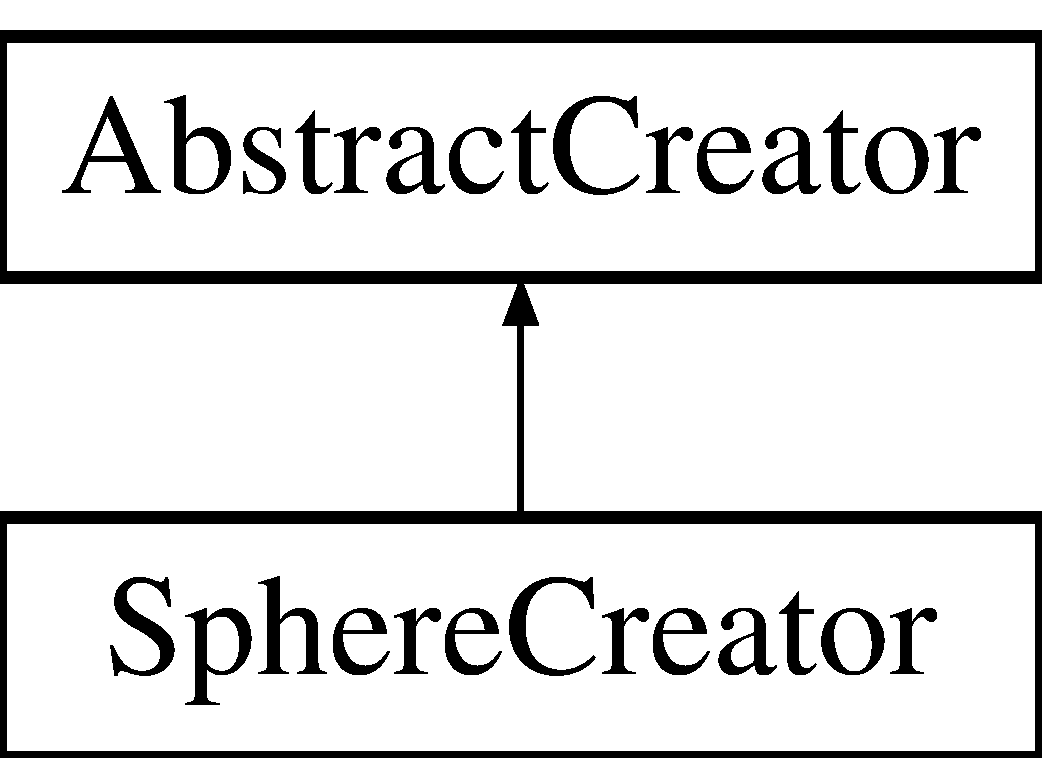
\includegraphics[height=2.000000cm]{d5/df1/class_sphere_creator}
\end{center}
\end{figure}
\subsection*{Public Member Functions}
\begin{DoxyCompactItemize}
\item 
\hyperlink{class_sphere_creator_a8fc063b81421021b1da0e77d57071cf6}{Sphere\+Creator} (vector$<$ double $>$ \hyperlink{class_sphere_creator_a4d3548be7ec07037e2d007dc07657de3}{center}, double \hyperlink{class_sphere_creator_aa0e357cf00720699cdaee04253ce492d}{radius}, double \hyperlink{class_sphere_creator_ae324f313bf48348001f328ea3abd9c7c}{phi\+Resolution}, double \hyperlink{class_sphere_creator_a062bf41868fd771016df76cb19550c36}{theta\+Resolution})
\item 
virtual \hyperlink{class_sphere_creator_a6e7073144b46c1988c2974689e5d1d21}{$\sim$\+Sphere\+Creator} ()
\item 
void \hyperlink{class_sphere_creator_a35e16f36b147b2fb2705d9413f5a963e}{create} (string filename)
\end{DoxyCompactItemize}
\subsection*{Private Attributes}
\begin{DoxyCompactItemize}
\item 
vector$<$ double $>$ \hyperlink{class_sphere_creator_a4d3548be7ec07037e2d007dc07657de3}{center}
\item 
double \hyperlink{class_sphere_creator_aa0e357cf00720699cdaee04253ce492d}{radius}
\item 
double \hyperlink{class_sphere_creator_ae324f313bf48348001f328ea3abd9c7c}{phi\+Resolution}
\item 
double \hyperlink{class_sphere_creator_a062bf41868fd771016df76cb19550c36}{theta\+Resolution}
\end{DoxyCompactItemize}


\subsection{Detailed Description}
Creates a V\+TP file containing a sphere. 

\subsection{Constructor \& Destructor Documentation}
\index{Sphere\+Creator@{Sphere\+Creator}!Sphere\+Creator@{Sphere\+Creator}}
\index{Sphere\+Creator@{Sphere\+Creator}!Sphere\+Creator@{Sphere\+Creator}}
\subsubsection[{\texorpdfstring{Sphere\+Creator(vector$<$ double $>$ center, double radius, double phi\+Resolution, double theta\+Resolution)}{SphereCreator(vector< double > center, double radius, double phiResolution, double thetaResolution)}}]{\setlength{\rightskip}{0pt plus 5cm}Sphere\+Creator\+::\+Sphere\+Creator (
\begin{DoxyParamCaption}
\item[{vector$<$ double $>$}]{center, }
\item[{double}]{radius, }
\item[{double}]{phi\+Resolution, }
\item[{double}]{theta\+Resolution}
\end{DoxyParamCaption}
)}\hypertarget{class_sphere_creator_a8fc063b81421021b1da0e77d57071cf6}{}\label{class_sphere_creator_a8fc063b81421021b1da0e77d57071cf6}
Initialize the inner variables of the object. 
\begin{DoxyParams}{Parameters}
{\em center} & 3D point denoting the center of the sphere. \\
\hline
{\em radius} & Radius of the sphere. \\
\hline
{\em phi\+Resolution} & Azimutal resolution of the sphere. \\
\hline
{\em theta\+Resolution} & Zenital resolution of the sphere. \\
\hline
\end{DoxyParams}
\index{Sphere\+Creator@{Sphere\+Creator}!````~Sphere\+Creator@{$\sim$\+Sphere\+Creator}}
\index{````~Sphere\+Creator@{$\sim$\+Sphere\+Creator}!Sphere\+Creator@{Sphere\+Creator}}
\subsubsection[{\texorpdfstring{$\sim$\+Sphere\+Creator()}{~SphereCreator()}}]{\setlength{\rightskip}{0pt plus 5cm}Sphere\+Creator\+::$\sim$\+Sphere\+Creator (
\begin{DoxyParamCaption}
{}
\end{DoxyParamCaption}
)\hspace{0.3cm}{\ttfamily [virtual]}}\hypertarget{class_sphere_creator_a6e7073144b46c1988c2974689e5d1d21}{}\label{class_sphere_creator_a6e7073144b46c1988c2974689e5d1d21}
Standard destructor. 

\subsection{Member Function Documentation}
\index{Sphere\+Creator@{Sphere\+Creator}!create@{create}}
\index{create@{create}!Sphere\+Creator@{Sphere\+Creator}}
\subsubsection[{\texorpdfstring{create(string filename)}{create(string filename)}}]{\setlength{\rightskip}{0pt plus 5cm}void Sphere\+Creator\+::create (
\begin{DoxyParamCaption}
\item[{string}]{filename}
\end{DoxyParamCaption}
)\hspace{0.3cm}{\ttfamily [virtual]}}\hypertarget{class_sphere_creator_a35e16f36b147b2fb2705d9413f5a963e}{}\label{class_sphere_creator_a35e16f36b147b2fb2705d9413f5a963e}
Persist the object in a file with V\+TP format. 
\begin{DoxyParams}{Parameters}
{\em filename} & Save file for the current object. \\
\hline
\end{DoxyParams}


Implements \hyperlink{class_abstract_creator_a1991e446444ffea2b85216b64f2dcf9e}{Abstract\+Creator}.



\subsection{Member Data Documentation}
\index{Sphere\+Creator@{Sphere\+Creator}!center@{center}}
\index{center@{center}!Sphere\+Creator@{Sphere\+Creator}}
\subsubsection[{\texorpdfstring{center}{center}}]{\setlength{\rightskip}{0pt plus 5cm}vector$<$double$>$ Sphere\+Creator\+::center\hspace{0.3cm}{\ttfamily [private]}}\hypertarget{class_sphere_creator_a4d3548be7ec07037e2d007dc07657de3}{}\label{class_sphere_creator_a4d3548be7ec07037e2d007dc07657de3}
3D point denoting the center of the sphere. \index{Sphere\+Creator@{Sphere\+Creator}!phi\+Resolution@{phi\+Resolution}}
\index{phi\+Resolution@{phi\+Resolution}!Sphere\+Creator@{Sphere\+Creator}}
\subsubsection[{\texorpdfstring{phi\+Resolution}{phiResolution}}]{\setlength{\rightskip}{0pt plus 5cm}double Sphere\+Creator\+::phi\+Resolution\hspace{0.3cm}{\ttfamily [private]}}\hypertarget{class_sphere_creator_ae324f313bf48348001f328ea3abd9c7c}{}\label{class_sphere_creator_ae324f313bf48348001f328ea3abd9c7c}
Azimutal resolution of the sphere. \index{Sphere\+Creator@{Sphere\+Creator}!radius@{radius}}
\index{radius@{radius}!Sphere\+Creator@{Sphere\+Creator}}
\subsubsection[{\texorpdfstring{radius}{radius}}]{\setlength{\rightskip}{0pt plus 5cm}double Sphere\+Creator\+::radius\hspace{0.3cm}{\ttfamily [private]}}\hypertarget{class_sphere_creator_aa0e357cf00720699cdaee04253ce492d}{}\label{class_sphere_creator_aa0e357cf00720699cdaee04253ce492d}
Radius of the sphere. \index{Sphere\+Creator@{Sphere\+Creator}!theta\+Resolution@{theta\+Resolution}}
\index{theta\+Resolution@{theta\+Resolution}!Sphere\+Creator@{Sphere\+Creator}}
\subsubsection[{\texorpdfstring{theta\+Resolution}{thetaResolution}}]{\setlength{\rightskip}{0pt plus 5cm}double Sphere\+Creator\+::theta\+Resolution\hspace{0.3cm}{\ttfamily [private]}}\hypertarget{class_sphere_creator_a062bf41868fd771016df76cb19550c36}{}\label{class_sphere_creator_a062bf41868fd771016df76cb19550c36}
Zenital resolution of the sphere. 

The documentation for this class was generated from the following files\+:\begin{DoxyCompactItemize}
\item 
creators/Sphere\+Creator.\+h\item 
creators/Sphere\+Creator.\+cpp\end{DoxyCompactItemize}

\hypertarget{class_sprouting_volumetric_cost_estimator}{}\section{Sprouting\+Volumetric\+Cost\+Estimator Class Reference}
\label{class_sprouting_volumetric_cost_estimator}\index{Sprouting\+Volumetric\+Cost\+Estimator@{Sprouting\+Volumetric\+Cost\+Estimator}}


{\ttfamily \#include $<$Sprouting\+Volumetric\+Cost\+Estimator.\+h$>$}

Inheritance diagram for Sprouting\+Volumetric\+Cost\+Estimator\+:\begin{figure}[H]
\begin{center}
\leavevmode
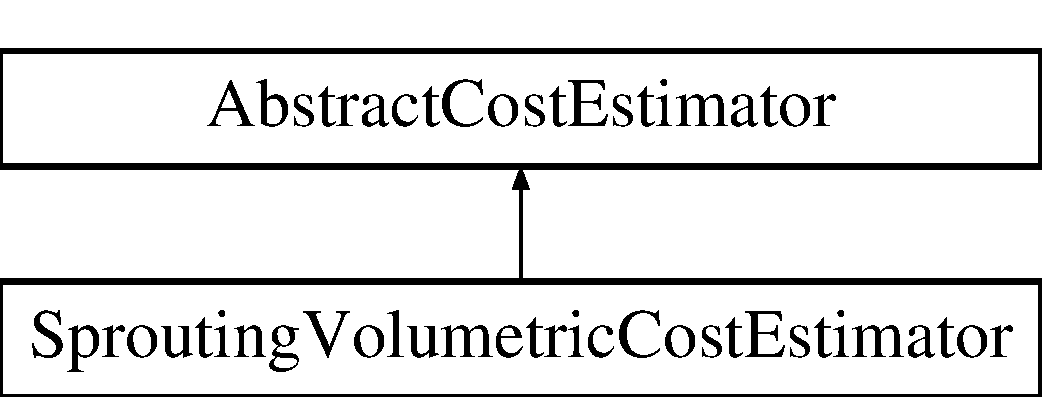
\includegraphics[height=2.000000cm]{d9/d05/class_sprouting_volumetric_cost_estimator}
\end{center}
\end{figure}
\subsection*{Public Member Functions}
\begin{DoxyCompactItemize}
\item 
\hyperlink{class_sprouting_volumetric_cost_estimator_ad6ad29e2e106454a64efa8d96451a1e7}{Sprouting\+Volumetric\+Cost\+Estimator} (double \hyperlink{class_sprouting_volumetric_cost_estimator_ae0a2bc9b3f1b08ff1b69367a638452fe}{volume\+Factor}, double \hyperlink{class_sprouting_volumetric_cost_estimator_a9bedc9f85b7b98700fd977bfbe956a33}{proteolytic\+Factor}, double \hyperlink{class_sprouting_volumetric_cost_estimator_afe49d902defafd1c47bd5c0ac39580cf}{diffusion\+Factor})
\item 
virtual \hyperlink{class_sprouting_volumetric_cost_estimator_a2931866fa094312a56209241970596fb}{$\sim$\+Sprouting\+Volumetric\+Cost\+Estimator} ()
\item 
\hyperlink{class_abstract_cost_estimator}{Abstract\+Cost\+Estimator} $\ast$ \hyperlink{class_sprouting_volumetric_cost_estimator_a9adf0950cceb8f82d66639bdabda6043}{clone} ()
\item 
void \hyperlink{class_sprouting_volumetric_cost_estimator_a712cbceabb8a8f63521af8d31010f955}{previous\+State} (\hyperlink{class_abstract_object_c_c_o_tree}{Abstract\+Object\+C\+C\+O\+Tree} $\ast$tree, \hyperlink{class_abstract_vascular_element}{Abstract\+Vascular\+Element} $\ast$parent, \hyperlink{structpoint}{point} i\+New, \hyperlink{structpoint}{point} i\+Test, double d\+Lim)
\item 
double \hyperlink{class_sprouting_volumetric_cost_estimator_ab301bfd1c1a93aa0f7535f268499dc63}{compute\+Cost} (\hyperlink{class_abstract_object_c_c_o_tree}{Abstract\+Object\+C\+C\+O\+Tree} $\ast$tree)
\end{DoxyCompactItemize}
\subsection*{Private Member Functions}
\begin{DoxyCompactItemize}
\item 
double \hyperlink{class_sprouting_volumetric_cost_estimator_a0a8f5cb6b80ec26f6025c430372f58cf}{compute\+Tree\+Cost} (\hyperlink{class_abstract_vascular_element}{Abstract\+Vascular\+Element} $\ast$root)
\end{DoxyCompactItemize}
\subsection*{Private Attributes}
\begin{DoxyCompactItemize}
\item 
double \hyperlink{class_sprouting_volumetric_cost_estimator_af63fec9f1deab61aadd3f5f2889956a2}{previous\+Volume}
\item 
double \hyperlink{class_sprouting_volumetric_cost_estimator_a9bedc9f85b7b98700fd977bfbe956a33}{proteolytic\+Factor}
\item 
double \hyperlink{class_sprouting_volumetric_cost_estimator_afe49d902defafd1c47bd5c0ac39580cf}{diffusion\+Factor}
\item 
double \hyperlink{class_sprouting_volumetric_cost_estimator_ae0a2bc9b3f1b08ff1b69367a638452fe}{volume\+Factor}
\item 
double \hyperlink{class_sprouting_volumetric_cost_estimator_af607b0ebd1aad6a5106c24cbd4452bd5}{dist\+To\+Parent}
\item 
double \hyperlink{class_sprouting_volumetric_cost_estimator_a4244e87579d0ff6b989ef221fff16187}{parent\+Radius}
\end{DoxyCompactItemize}


\subsection{Detailed Description}
Cost estimator that considers diffusion and vessel wall degradation associated to sprouting angiogenesis and also weighs the variation of the tree volume. 

\subsection{Constructor \& Destructor Documentation}
\index{Sprouting\+Volumetric\+Cost\+Estimator@{Sprouting\+Volumetric\+Cost\+Estimator}!Sprouting\+Volumetric\+Cost\+Estimator@{Sprouting\+Volumetric\+Cost\+Estimator}}
\index{Sprouting\+Volumetric\+Cost\+Estimator@{Sprouting\+Volumetric\+Cost\+Estimator}!Sprouting\+Volumetric\+Cost\+Estimator@{Sprouting\+Volumetric\+Cost\+Estimator}}
\subsubsection[{\texorpdfstring{Sprouting\+Volumetric\+Cost\+Estimator(double volume\+Factor, double proteolytic\+Factor, double diffusion\+Factor)}{SproutingVolumetricCostEstimator(double volumeFactor, double proteolyticFactor, double diffusionFactor)}}]{\setlength{\rightskip}{0pt plus 5cm}Sprouting\+Volumetric\+Cost\+Estimator\+::\+Sprouting\+Volumetric\+Cost\+Estimator (
\begin{DoxyParamCaption}
\item[{double}]{volume\+Factor, }
\item[{double}]{proteolytic\+Factor, }
\item[{double}]{diffusion\+Factor}
\end{DoxyParamCaption}
)}\hypertarget{class_sprouting_volumetric_cost_estimator_ad6ad29e2e106454a64efa8d96451a1e7}{}\label{class_sprouting_volumetric_cost_estimator_ad6ad29e2e106454a64efa8d96451a1e7}
Common constructor. \index{Sprouting\+Volumetric\+Cost\+Estimator@{Sprouting\+Volumetric\+Cost\+Estimator}!````~Sprouting\+Volumetric\+Cost\+Estimator@{$\sim$\+Sprouting\+Volumetric\+Cost\+Estimator}}
\index{````~Sprouting\+Volumetric\+Cost\+Estimator@{$\sim$\+Sprouting\+Volumetric\+Cost\+Estimator}!Sprouting\+Volumetric\+Cost\+Estimator@{Sprouting\+Volumetric\+Cost\+Estimator}}
\subsubsection[{\texorpdfstring{$\sim$\+Sprouting\+Volumetric\+Cost\+Estimator()}{~SproutingVolumetricCostEstimator()}}]{\setlength{\rightskip}{0pt plus 5cm}Sprouting\+Volumetric\+Cost\+Estimator\+::$\sim$\+Sprouting\+Volumetric\+Cost\+Estimator (
\begin{DoxyParamCaption}
{}
\end{DoxyParamCaption}
)\hspace{0.3cm}{\ttfamily [virtual]}}\hypertarget{class_sprouting_volumetric_cost_estimator_a2931866fa094312a56209241970596fb}{}\label{class_sprouting_volumetric_cost_estimator_a2931866fa094312a56209241970596fb}
Common destructor. 

\subsection{Member Function Documentation}
\index{Sprouting\+Volumetric\+Cost\+Estimator@{Sprouting\+Volumetric\+Cost\+Estimator}!clone@{clone}}
\index{clone@{clone}!Sprouting\+Volumetric\+Cost\+Estimator@{Sprouting\+Volumetric\+Cost\+Estimator}}
\subsubsection[{\texorpdfstring{clone()}{clone()}}]{\setlength{\rightskip}{0pt plus 5cm}{\bf Abstract\+Cost\+Estimator} $\ast$ Sprouting\+Volumetric\+Cost\+Estimator\+::clone (
\begin{DoxyParamCaption}
{}
\end{DoxyParamCaption}
)\hspace{0.3cm}{\ttfamily [virtual]}}\hypertarget{class_sprouting_volumetric_cost_estimator_a9adf0950cceb8f82d66639bdabda6043}{}\label{class_sprouting_volumetric_cost_estimator_a9adf0950cceb8f82d66639bdabda6043}
Clones the current estimator instance. \begin{DoxyReturn}{Returns}
Cloned instance. 
\end{DoxyReturn}


Implements \hyperlink{class_abstract_cost_estimator_a928e53418b17eb68c443e2a68fe5cbcf}{Abstract\+Cost\+Estimator}.

\index{Sprouting\+Volumetric\+Cost\+Estimator@{Sprouting\+Volumetric\+Cost\+Estimator}!compute\+Cost@{compute\+Cost}}
\index{compute\+Cost@{compute\+Cost}!Sprouting\+Volumetric\+Cost\+Estimator@{Sprouting\+Volumetric\+Cost\+Estimator}}
\subsubsection[{\texorpdfstring{compute\+Cost(\+Abstract\+Object\+C\+C\+O\+Tree $\ast$tree)}{computeCost(AbstractObjectCCOTree *tree)}}]{\setlength{\rightskip}{0pt plus 5cm}double Sprouting\+Volumetric\+Cost\+Estimator\+::compute\+Cost (
\begin{DoxyParamCaption}
\item[{{\bf Abstract\+Object\+C\+C\+O\+Tree} $\ast$}]{tree}
\end{DoxyParamCaption}
)\hspace{0.3cm}{\ttfamily [virtual]}}\hypertarget{class_sprouting_volumetric_cost_estimator_ab301bfd1c1a93aa0f7535f268499dc63}{}\label{class_sprouting_volumetric_cost_estimator_ab301bfd1c1a93aa0f7535f268499dc63}
Computes the functional cost of the given tree. 
\begin{DoxyParams}{Parameters}
{\em tree} & Tree at the current step. \\
\hline
\end{DoxyParams}
\begin{DoxyReturn}{Returns}
Cost of the given tree. 
\end{DoxyReturn}


Implements \hyperlink{class_abstract_cost_estimator_a2be0c6cc4aa6a73110c75ad903af428e}{Abstract\+Cost\+Estimator}.

\index{Sprouting\+Volumetric\+Cost\+Estimator@{Sprouting\+Volumetric\+Cost\+Estimator}!compute\+Tree\+Cost@{compute\+Tree\+Cost}}
\index{compute\+Tree\+Cost@{compute\+Tree\+Cost}!Sprouting\+Volumetric\+Cost\+Estimator@{Sprouting\+Volumetric\+Cost\+Estimator}}
\subsubsection[{\texorpdfstring{compute\+Tree\+Cost(\+Abstract\+Vascular\+Element $\ast$root)}{computeTreeCost(AbstractVascularElement *root)}}]{\setlength{\rightskip}{0pt plus 5cm}double Sprouting\+Volumetric\+Cost\+Estimator\+::compute\+Tree\+Cost (
\begin{DoxyParamCaption}
\item[{{\bf Abstract\+Vascular\+Element} $\ast$}]{root}
\end{DoxyParamCaption}
)\hspace{0.3cm}{\ttfamily [private]}}\hypertarget{class_sprouting_volumetric_cost_estimator_a0a8f5cb6b80ec26f6025c430372f58cf}{}\label{class_sprouting_volumetric_cost_estimator_a0a8f5cb6b80ec26f6025c430372f58cf}
Computes the volume for the tree with root {\ttfamily root}. 
\begin{DoxyParams}{Parameters}
{\em root} & Root of the tree. \\
\hline
\end{DoxyParams}
\begin{DoxyReturn}{Returns}
Volume of the tree. 
\end{DoxyReturn}
\index{Sprouting\+Volumetric\+Cost\+Estimator@{Sprouting\+Volumetric\+Cost\+Estimator}!previous\+State@{previous\+State}}
\index{previous\+State@{previous\+State}!Sprouting\+Volumetric\+Cost\+Estimator@{Sprouting\+Volumetric\+Cost\+Estimator}}
\subsubsection[{\texorpdfstring{previous\+State(\+Abstract\+Object\+C\+C\+O\+Tree $\ast$tree, Abstract\+Vascular\+Element $\ast$parent, point i\+New, point i\+Test, double d\+Lim)}{previousState(AbstractObjectCCOTree *tree, AbstractVascularElement *parent, point iNew, point iTest, double dLim)}}]{\setlength{\rightskip}{0pt plus 5cm}void Sprouting\+Volumetric\+Cost\+Estimator\+::previous\+State (
\begin{DoxyParamCaption}
\item[{{\bf Abstract\+Object\+C\+C\+O\+Tree} $\ast$}]{tree, }
\item[{{\bf Abstract\+Vascular\+Element} $\ast$}]{parent, }
\item[{{\bf point}}]{i\+New, }
\item[{{\bf point}}]{i\+Test, }
\item[{double}]{d\+Lim}
\end{DoxyParamCaption}
)\hspace{0.3cm}{\ttfamily [virtual]}}\hypertarget{class_sprouting_volumetric_cost_estimator_a712cbceabb8a8f63521af8d31010f955}{}\label{class_sprouting_volumetric_cost_estimator_a712cbceabb8a8f63521af8d31010f955}
Extracts information of the tree at the previous step. 
\begin{DoxyParams}{Parameters}
{\em root} & Root of the tree at the previous step. \\
\hline
{\em parent} & Vascular element where the new vessel will be connected. \\
\hline
{\em i\+New} & Distal position of the new vessel. \\
\hline
{\em i\+Test} & Proximal position of the new vessel. \\
\hline
{\em d\+Lim} & Minimum radius distance from the new vessel to the tree. \\
\hline
\end{DoxyParams}


Implements \hyperlink{class_abstract_cost_estimator_a8a806c3e4537c6d4acc428b029fd60de}{Abstract\+Cost\+Estimator}.



\subsection{Member Data Documentation}
\index{Sprouting\+Volumetric\+Cost\+Estimator@{Sprouting\+Volumetric\+Cost\+Estimator}!diffusion\+Factor@{diffusion\+Factor}}
\index{diffusion\+Factor@{diffusion\+Factor}!Sprouting\+Volumetric\+Cost\+Estimator@{Sprouting\+Volumetric\+Cost\+Estimator}}
\subsubsection[{\texorpdfstring{diffusion\+Factor}{diffusionFactor}}]{\setlength{\rightskip}{0pt plus 5cm}double Sprouting\+Volumetric\+Cost\+Estimator\+::diffusion\+Factor\hspace{0.3cm}{\ttfamily [private]}}\hypertarget{class_sprouting_volumetric_cost_estimator_afe49d902defafd1c47bd5c0ac39580cf}{}\label{class_sprouting_volumetric_cost_estimator_afe49d902defafd1c47bd5c0ac39580cf}
Factor of media diffusion of angiogenic growth factors. \index{Sprouting\+Volumetric\+Cost\+Estimator@{Sprouting\+Volumetric\+Cost\+Estimator}!dist\+To\+Parent@{dist\+To\+Parent}}
\index{dist\+To\+Parent@{dist\+To\+Parent}!Sprouting\+Volumetric\+Cost\+Estimator@{Sprouting\+Volumetric\+Cost\+Estimator}}
\subsubsection[{\texorpdfstring{dist\+To\+Parent}{distToParent}}]{\setlength{\rightskip}{0pt plus 5cm}double Sprouting\+Volumetric\+Cost\+Estimator\+::dist\+To\+Parent\hspace{0.3cm}{\ttfamily [private]}}\hypertarget{class_sprouting_volumetric_cost_estimator_af607b0ebd1aad6a5106c24cbd4452bd5}{}\label{class_sprouting_volumetric_cost_estimator_af607b0ebd1aad6a5106c24cbd4452bd5}
Distance between sprouting source and candidate parent vessel. \index{Sprouting\+Volumetric\+Cost\+Estimator@{Sprouting\+Volumetric\+Cost\+Estimator}!parent\+Radius@{parent\+Radius}}
\index{parent\+Radius@{parent\+Radius}!Sprouting\+Volumetric\+Cost\+Estimator@{Sprouting\+Volumetric\+Cost\+Estimator}}
\subsubsection[{\texorpdfstring{parent\+Radius}{parentRadius}}]{\setlength{\rightskip}{0pt plus 5cm}double Sprouting\+Volumetric\+Cost\+Estimator\+::parent\+Radius\hspace{0.3cm}{\ttfamily [private]}}\hypertarget{class_sprouting_volumetric_cost_estimator_a4244e87579d0ff6b989ef221fff16187}{}\label{class_sprouting_volumetric_cost_estimator_a4244e87579d0ff6b989ef221fff16187}
Radius of the candidate parent vessel. \index{Sprouting\+Volumetric\+Cost\+Estimator@{Sprouting\+Volumetric\+Cost\+Estimator}!previous\+Volume@{previous\+Volume}}
\index{previous\+Volume@{previous\+Volume}!Sprouting\+Volumetric\+Cost\+Estimator@{Sprouting\+Volumetric\+Cost\+Estimator}}
\subsubsection[{\texorpdfstring{previous\+Volume}{previousVolume}}]{\setlength{\rightskip}{0pt plus 5cm}double Sprouting\+Volumetric\+Cost\+Estimator\+::previous\+Volume\hspace{0.3cm}{\ttfamily [private]}}\hypertarget{class_sprouting_volumetric_cost_estimator_af63fec9f1deab61aadd3f5f2889956a2}{}\label{class_sprouting_volumetric_cost_estimator_af63fec9f1deab61aadd3f5f2889956a2}
Volume at the previous step. \index{Sprouting\+Volumetric\+Cost\+Estimator@{Sprouting\+Volumetric\+Cost\+Estimator}!proteolytic\+Factor@{proteolytic\+Factor}}
\index{proteolytic\+Factor@{proteolytic\+Factor}!Sprouting\+Volumetric\+Cost\+Estimator@{Sprouting\+Volumetric\+Cost\+Estimator}}
\subsubsection[{\texorpdfstring{proteolytic\+Factor}{proteolyticFactor}}]{\setlength{\rightskip}{0pt plus 5cm}double Sprouting\+Volumetric\+Cost\+Estimator\+::proteolytic\+Factor\hspace{0.3cm}{\ttfamily [private]}}\hypertarget{class_sprouting_volumetric_cost_estimator_a9bedc9f85b7b98700fd977bfbe956a33}{}\label{class_sprouting_volumetric_cost_estimator_a9bedc9f85b7b98700fd977bfbe956a33}
Vessel wall proteolytic degradation factor. \index{Sprouting\+Volumetric\+Cost\+Estimator@{Sprouting\+Volumetric\+Cost\+Estimator}!volume\+Factor@{volume\+Factor}}
\index{volume\+Factor@{volume\+Factor}!Sprouting\+Volumetric\+Cost\+Estimator@{Sprouting\+Volumetric\+Cost\+Estimator}}
\subsubsection[{\texorpdfstring{volume\+Factor}{volumeFactor}}]{\setlength{\rightskip}{0pt plus 5cm}double Sprouting\+Volumetric\+Cost\+Estimator\+::volume\+Factor\hspace{0.3cm}{\ttfamily [private]}}\hypertarget{class_sprouting_volumetric_cost_estimator_ae0a2bc9b3f1b08ff1b69367a638452fe}{}\label{class_sprouting_volumetric_cost_estimator_ae0a2bc9b3f1b08ff1b69367a638452fe}
Weigh for tree volume. 

The documentation for this class was generated from the following files\+:\begin{DoxyCompactItemize}
\item 
structures/tree/Sprouting\+Volumetric\+Cost\+Estimator.\+h\item 
structures/tree/Sprouting\+Volumetric\+Cost\+Estimator.\+cpp\end{DoxyCompactItemize}

\hypertarget{class_staged_domain}{}\section{Staged\+Domain Class Reference}
\label{class_staged_domain}\index{Staged\+Domain@{Staged\+Domain}}


{\ttfamily \#include $<$Staged\+Domain.\+h$>$}

Inheritance diagram for Staged\+Domain\+:\begin{figure}[H]
\begin{center}
\leavevmode
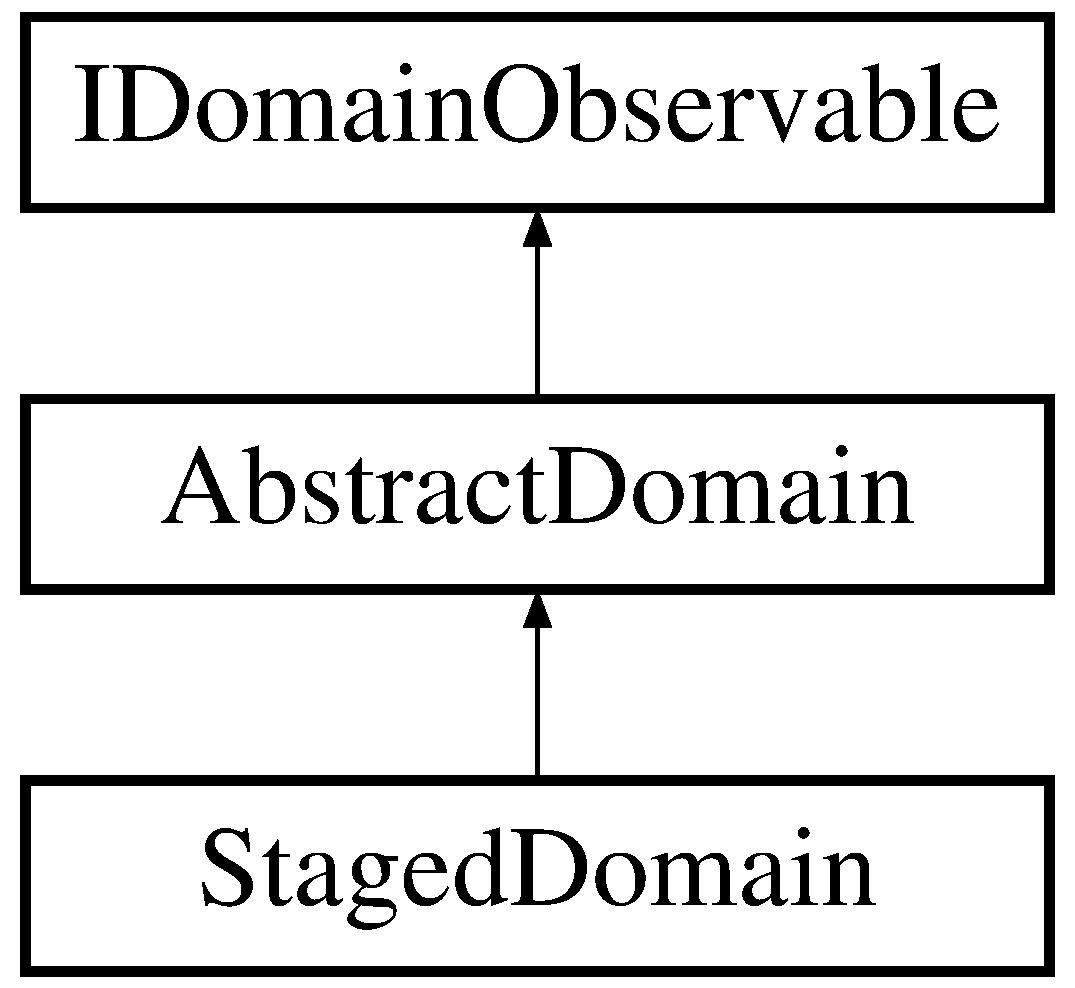
\includegraphics[height=3.000000cm]{d2/d7b/class_staged_domain}
\end{center}
\end{figure}
\subsection*{Public Member Functions}
\begin{DoxyCompactItemize}
\item 
\hyperlink{class_staged_domain_a48d3fc928f1c52c13adc66761fd45353}{Staged\+Domain} ()
\item 
void \hyperlink{class_staged_domain_a3b206c2ba98d6fca73dd2b76689f9742}{add\+Stage} (long long int terminals, \hyperlink{class_abstract_domain}{Abstract\+Domain} $\ast$domain)
\item 
void \hyperlink{class_staged_domain_abacd2429b605ac8ae9c94701485f4df0}{update} ()
\item 
long long int \hyperlink{class_staged_domain_ac179c1e1d0a2aac78093bd71d083811f}{get\+Terminals\+After\+Generation} ()
\item 
int \hyperlink{class_staged_domain_a2f13523c9e014efd270df926aabdbc76}{is\+Segment\+Inside} (\hyperlink{structpoint}{point} xs, \hyperlink{structpoint}{point} xf)
\item 
int \hyperlink{class_staged_domain_a083dae621ca3d910b23f5cd85ba23d65}{is\+Valid\+Element} (\hyperlink{class_abstract_vascular_element}{Abstract\+Vascular\+Element} $\ast$element)
\item 
double \hyperlink{class_staged_domain_aec389e04bcd549140b29dbc9c56cf29b}{get\+Characteristic\+Length} ()
\item 
double \hyperlink{class_staged_domain_a4bb50d4e92dc81e0c87aa0b4190138b3}{get\+D\+Lim} (long long int n\+Vessels, double factor)
\item 
double $\ast$ \hyperlink{class_staged_domain_ad8107b681fcba3794ea4cd9b1a5a2edd}{get\+Local\+Neighborhood} (\hyperlink{structpoint}{point} p, long long int n\+Vessels)
\item 
double \hyperlink{class_staged_domain_a139146506055f007980898b55fc894e0}{get\+Min\+Bifurcation\+Angle} ()
\item 
double \hyperlink{class_staged_domain_a211adf0d69765f74dc13c3219a670c00}{get\+Min\+Plane\+Angle} ()
\item 
double \hyperlink{class_staged_domain_a807d7b1c56b5a6ccce593513baebf3b1}{get\+Size} ()
\item 
\hyperlink{structpoint}{point} \hyperlink{class_staged_domain_a90178baeab98fe08850977e7924c2780}{get\+Random\+Point} ()
\item 
deque$<$ \hyperlink{structpoint}{point} $>$ \& \hyperlink{class_staged_domain_a5a5398712e064cbd706f701c8294bbad}{get\+Random\+Inner\+Points} ()
\item 
long long int \hyperlink{class_staged_domain_ac794500d0ba6b4a21cd30eeda13c0b5c}{get\+Point\+Counter} () const 
\item 
vtk\+Smart\+Pointer$<$ vtk\+Poly\+Data $>$ \& \hyperlink{class_staged_domain_a69530fd545f217410433367a7e219fbf}{get\+Vtk\+Geometry} ()
\item 
int \hyperlink{class_staged_domain_a9483ed1fc5df7381f739ade92c92444f}{get\+Current\+Stage} () const 
\item 
void \hyperlink{class_staged_domain_a58e3ccb3449324920bc187bf8921b238}{set\+Initial\+Stage} (int \hyperlink{class_staged_domain_a0fc23a88dcfb07e4a2b5d3899811a2a6}{current\+Stage})
\end{DoxyCompactItemize}
\subsection*{Private Attributes}
\begin{DoxyCompactItemize}
\item 
vector$<$ \hyperlink{class_abstract_domain}{Abstract\+Domain} $\ast$ $>$ \hyperlink{class_staged_domain_a3372c80d0c3bff5255c0d4a7bbce3647}{domain\+Stage}
\item 
vector$<$ long long int $>$ \hyperlink{class_staged_domain_a8ca1e0466a1ba6563cbe103ac4499364}{terminals\+Per\+Stage}
\item 
long long int \hyperlink{class_staged_domain_a8383f99269b421f85b89c3aa847f91ce}{current\+Terminals}
\item 
long long int \hyperlink{class_staged_domain_a94b7ffac4fc6e07fc14061cdf68475b7}{terminal\+At\+Prev\+Stage}
\item 
int \hyperlink{class_staged_domain_a0fc23a88dcfb07e4a2b5d3899811a2a6}{current\+Stage}
\item 
int {\bfseries initial\+Stage}\hypertarget{class_staged_domain_aeb7e7a081ce55e7d715e317bcd34fbf7}{}\label{class_staged_domain_aeb7e7a081ce55e7d715e317bcd34fbf7}

\end{DoxyCompactItemize}
\subsection*{Additional Inherited Members}


\subsection{Detailed Description}
Composite class that modify the domain depending in the amount of terminals that have been included. 

\subsection{Constructor \& Destructor Documentation}
\index{Staged\+Domain@{Staged\+Domain}!Staged\+Domain@{Staged\+Domain}}
\index{Staged\+Domain@{Staged\+Domain}!Staged\+Domain@{Staged\+Domain}}
\subsubsection[{\texorpdfstring{Staged\+Domain()}{StagedDomain()}}]{\setlength{\rightskip}{0pt plus 5cm}Staged\+Domain\+::\+Staged\+Domain (
\begin{DoxyParamCaption}
{}
\end{DoxyParamCaption}
)}\hypertarget{class_staged_domain_a48d3fc928f1c52c13adc66761fd45353}{}\label{class_staged_domain_a48d3fc928f1c52c13adc66761fd45353}
Constructor. 

\subsection{Member Function Documentation}
\index{Staged\+Domain@{Staged\+Domain}!add\+Stage@{add\+Stage}}
\index{add\+Stage@{add\+Stage}!Staged\+Domain@{Staged\+Domain}}
\subsubsection[{\texorpdfstring{add\+Stage(long long int terminals, Abstract\+Domain $\ast$domain)}{addStage(long long int terminals, AbstractDomain *domain)}}]{\setlength{\rightskip}{0pt plus 5cm}void Staged\+Domain\+::add\+Stage (
\begin{DoxyParamCaption}
\item[{long long int}]{terminals, }
\item[{{\bf Abstract\+Domain} $\ast$}]{domain}
\end{DoxyParamCaption}
)}\hypertarget{class_staged_domain_a3b206c2ba98d6fca73dd2b76689f9742}{}\label{class_staged_domain_a3b206c2ba98d6fca73dd2b76689f9742}
Add an additional stage to the domain. 
\begin{DoxyParams}{Parameters}
{\em terminals} & Amount of terminals for the added stage. \\
\hline
{\em domain} & Domain used for the added stage. \\
\hline
\end{DoxyParams}
\index{Staged\+Domain@{Staged\+Domain}!get\+Characteristic\+Length@{get\+Characteristic\+Length}}
\index{get\+Characteristic\+Length@{get\+Characteristic\+Length}!Staged\+Domain@{Staged\+Domain}}
\subsubsection[{\texorpdfstring{get\+Characteristic\+Length()}{getCharacteristicLength()}}]{\setlength{\rightskip}{0pt plus 5cm}double Staged\+Domain\+::get\+Characteristic\+Length (
\begin{DoxyParamCaption}
{}
\end{DoxyParamCaption}
)\hspace{0.3cm}{\ttfamily [virtual]}}\hypertarget{class_staged_domain_aec389e04bcd549140b29dbc9c56cf29b}{}\label{class_staged_domain_aec389e04bcd549140b29dbc9c56cf29b}
Estimates a characteristic length for the current domain. This length is useful to estimate the perfusion volume of the domain. \begin{DoxyReturn}{Returns}
Chracteristic length. 
\end{DoxyReturn}


Implements \hyperlink{class_abstract_domain_a90ca3dff64bab2428da8ced24e16f4c3}{Abstract\+Domain}.

\index{Staged\+Domain@{Staged\+Domain}!get\+Current\+Stage@{get\+Current\+Stage}}
\index{get\+Current\+Stage@{get\+Current\+Stage}!Staged\+Domain@{Staged\+Domain}}
\subsubsection[{\texorpdfstring{get\+Current\+Stage() const }{getCurrentStage() const }}]{\setlength{\rightskip}{0pt plus 5cm}int Staged\+Domain\+::get\+Current\+Stage (
\begin{DoxyParamCaption}
{}
\end{DoxyParamCaption}
) const}\hypertarget{class_staged_domain_a9483ed1fc5df7381f739ade92c92444f}{}\label{class_staged_domain_a9483ed1fc5df7381f739ade92c92444f}
Returns the current stage. \begin{DoxyReturn}{Returns}
Current stage number; 
\end{DoxyReturn}
\index{Staged\+Domain@{Staged\+Domain}!get\+D\+Lim@{get\+D\+Lim}}
\index{get\+D\+Lim@{get\+D\+Lim}!Staged\+Domain@{Staged\+Domain}}
\subsubsection[{\texorpdfstring{get\+D\+Lim(long long int n\+Vessels, double factor)}{getDLim(long long int nVessels, double factor)}}]{\setlength{\rightskip}{0pt plus 5cm}double Staged\+Domain\+::get\+D\+Lim (
\begin{DoxyParamCaption}
\item[{long long int}]{n\+Vessels, }
\item[{double}]{factor}
\end{DoxyParamCaption}
)\hspace{0.3cm}{\ttfamily [virtual]}}\hypertarget{class_staged_domain_a4bb50d4e92dc81e0c87aa0b4190138b3}{}\label{class_staged_domain_a4bb50d4e92dc81e0c87aa0b4190138b3}
Minimum distance between a new vessel terminal and the tree based on the current terminal perfusion. This is lower bound criteria for the vessel length and also aids toward a spatially homogeneous terminal distribution. 
\begin{DoxyParams}{Parameters}
{\em n\+Vessels} & Quantity of terminals in the current tree. \\
\hline
{\em factor} & Factor used to scale a perfusion measure in order to estimate the D\+Lim value. \\
\hline
\end{DoxyParams}
\begin{DoxyReturn}{Returns}
D\+Lim value. 
\end{DoxyReturn}


Implements \hyperlink{class_abstract_domain_ac9f39c12182608eb704c051e5d1cbc55}{Abstract\+Domain}.

\index{Staged\+Domain@{Staged\+Domain}!get\+Local\+Neighborhood@{get\+Local\+Neighborhood}}
\index{get\+Local\+Neighborhood@{get\+Local\+Neighborhood}!Staged\+Domain@{Staged\+Domain}}
\subsubsection[{\texorpdfstring{get\+Local\+Neighborhood(point p, long long int n\+Vessels)}{getLocalNeighborhood(point p, long long int nVessels)}}]{\setlength{\rightskip}{0pt plus 5cm}double $\ast$ Staged\+Domain\+::get\+Local\+Neighborhood (
\begin{DoxyParamCaption}
\item[{{\bf point}}]{p, }
\item[{long long int}]{n\+Vessels}
\end{DoxyParamCaption}
)\hspace{0.3cm}{\ttfamily [virtual]}}\hypertarget{class_staged_domain_ad8107b681fcba3794ea4cd9b1a5a2edd}{}\label{class_staged_domain_ad8107b681fcba3794ea4cd9b1a5a2edd}
Returns the local neighbors to the {\ttfamily p} point locus. The amount of neighbors is estimated based on the current terminal perfusion. 
\begin{DoxyParams}{Parameters}
{\em p} & Central point of the neighborhood. \\
\hline
{\em n\+Vessels} & Amount of terminals in the tree. \\
\hline
\end{DoxyParams}
\begin{DoxyReturn}{Returns}
Array of neighbor vessels. 
\end{DoxyReturn}


Implements \hyperlink{class_abstract_domain_aee2b549d19062b261429f8a442fb4714}{Abstract\+Domain}.

\index{Staged\+Domain@{Staged\+Domain}!get\+Min\+Bifurcation\+Angle@{get\+Min\+Bifurcation\+Angle}}
\index{get\+Min\+Bifurcation\+Angle@{get\+Min\+Bifurcation\+Angle}!Staged\+Domain@{Staged\+Domain}}
\subsubsection[{\texorpdfstring{get\+Min\+Bifurcation\+Angle()}{getMinBifurcationAngle()}}]{\setlength{\rightskip}{0pt plus 5cm}double Staged\+Domain\+::get\+Min\+Bifurcation\+Angle (
\begin{DoxyParamCaption}
{}
\end{DoxyParamCaption}
)\hspace{0.3cm}{\ttfamily [virtual]}}\hypertarget{class_staged_domain_a139146506055f007980898b55fc894e0}{}\label{class_staged_domain_a139146506055f007980898b55fc894e0}
Returns the maximum angle that the hosted tree can generate. \begin{DoxyReturn}{Returns}
Maximum bifurcation angle for vessels generated inside this domain. 
\end{DoxyReturn}


Reimplemented from \hyperlink{class_abstract_domain_a434417bad2396a2ee600932d1d2ded89}{Abstract\+Domain}.

\index{Staged\+Domain@{Staged\+Domain}!get\+Min\+Plane\+Angle@{get\+Min\+Plane\+Angle}}
\index{get\+Min\+Plane\+Angle@{get\+Min\+Plane\+Angle}!Staged\+Domain@{Staged\+Domain}}
\subsubsection[{\texorpdfstring{get\+Min\+Plane\+Angle()}{getMinPlaneAngle()}}]{\setlength{\rightskip}{0pt plus 5cm}double Staged\+Domain\+::get\+Min\+Plane\+Angle (
\begin{DoxyParamCaption}
{}
\end{DoxyParamCaption}
)}\hypertarget{class_staged_domain_a211adf0d69765f74dc13c3219a670c00}{}\label{class_staged_domain_a211adf0d69765f74dc13c3219a670c00}
Returns the maximum opening angle that the hosted tree can generate. \begin{DoxyReturn}{Returns}
Maximum opening angle for vessels generated inside this domain. 
\end{DoxyReturn}
\index{Staged\+Domain@{Staged\+Domain}!get\+Point\+Counter@{get\+Point\+Counter}}
\index{get\+Point\+Counter@{get\+Point\+Counter}!Staged\+Domain@{Staged\+Domain}}
\subsubsection[{\texorpdfstring{get\+Point\+Counter() const }{getPointCounter() const }}]{\setlength{\rightskip}{0pt plus 5cm}long long int Staged\+Domain\+::get\+Point\+Counter (
\begin{DoxyParamCaption}
{}
\end{DoxyParamCaption}
) const}\hypertarget{class_staged_domain_ac794500d0ba6b4a21cd30eeda13c0b5c}{}\label{class_staged_domain_ac794500d0ba6b4a21cd30eeda13c0b5c}
Returns the quantity of points that have been consumed. \begin{DoxyReturn}{Returns}
Quantity of points consumed. 
\end{DoxyReturn}
\index{Staged\+Domain@{Staged\+Domain}!get\+Random\+Inner\+Points@{get\+Random\+Inner\+Points}}
\index{get\+Random\+Inner\+Points@{get\+Random\+Inner\+Points}!Staged\+Domain@{Staged\+Domain}}
\subsubsection[{\texorpdfstring{get\+Random\+Inner\+Points()}{getRandomInnerPoints()}}]{\setlength{\rightskip}{0pt plus 5cm}deque$<$ {\bf point} $>$ \& Staged\+Domain\+::get\+Random\+Inner\+Points (
\begin{DoxyParamCaption}
{}
\end{DoxyParamCaption}
)\hspace{0.3cm}{\ttfamily [virtual]}}\hypertarget{class_staged_domain_a5a5398712e064cbd706f701c8294bbad}{}\label{class_staged_domain_a5a5398712e064cbd706f701c8294bbad}
Return a set of inner domain points. \begin{DoxyReturn}{Returns}
Set of inner domain points. 
\end{DoxyReturn}


Implements \hyperlink{class_abstract_domain_a73d2c0e7c670b007bb5dbbdab5ad6b1b}{Abstract\+Domain}.

\index{Staged\+Domain@{Staged\+Domain}!get\+Random\+Point@{get\+Random\+Point}}
\index{get\+Random\+Point@{get\+Random\+Point}!Staged\+Domain@{Staged\+Domain}}
\subsubsection[{\texorpdfstring{get\+Random\+Point()}{getRandomPoint()}}]{\setlength{\rightskip}{0pt plus 5cm}{\bf point} Staged\+Domain\+::get\+Random\+Point (
\begin{DoxyParamCaption}
{}
\end{DoxyParamCaption}
)\hspace{0.3cm}{\ttfamily [virtual]}}\hypertarget{class_staged_domain_a90178baeab98fe08850977e7924c2780}{}\label{class_staged_domain_a90178baeab98fe08850977e7924c2780}
Return a random point inside the domain. \begin{DoxyReturn}{Returns}
Point inside the domain. 
\end{DoxyReturn}


Implements \hyperlink{class_abstract_domain_ae31a5b26d1dc628abe24da7a4d375415}{Abstract\+Domain}.

\index{Staged\+Domain@{Staged\+Domain}!get\+Size@{get\+Size}}
\index{get\+Size@{get\+Size}!Staged\+Domain@{Staged\+Domain}}
\subsubsection[{\texorpdfstring{get\+Size()}{getSize()}}]{\setlength{\rightskip}{0pt plus 5cm}double Staged\+Domain\+::get\+Size (
\begin{DoxyParamCaption}
{}
\end{DoxyParamCaption}
)\hspace{0.3cm}{\ttfamily [virtual]}}\hypertarget{class_staged_domain_a807d7b1c56b5a6ccce593513baebf3b1}{}\label{class_staged_domain_a807d7b1c56b5a6ccce593513baebf3b1}
Computes the size of the domain. \begin{DoxyReturn}{Returns}
Size of the domain. 
\end{DoxyReturn}


Implements \hyperlink{class_abstract_domain_a049564d82f2c177c39834dfc8da143dc}{Abstract\+Domain}.

\index{Staged\+Domain@{Staged\+Domain}!get\+Terminals\+After\+Generation@{get\+Terminals\+After\+Generation}}
\index{get\+Terminals\+After\+Generation@{get\+Terminals\+After\+Generation}!Staged\+Domain@{Staged\+Domain}}
\subsubsection[{\texorpdfstring{get\+Terminals\+After\+Generation()}{getTerminalsAfterGeneration()}}]{\setlength{\rightskip}{0pt plus 5cm}long long int Staged\+Domain\+::get\+Terminals\+After\+Generation (
\begin{DoxyParamCaption}
{}
\end{DoxyParamCaption}
)}\hypertarget{class_staged_domain_ac179c1e1d0a2aac78093bd71d083811f}{}\label{class_staged_domain_ac179c1e1d0a2aac78093bd71d083811f}
Returns the total amount of terminals that will be generated along all stages. \begin{DoxyReturn}{Returns}
Total amount of terminals generated along all stages. 
\end{DoxyReturn}
\index{Staged\+Domain@{Staged\+Domain}!get\+Vtk\+Geometry@{get\+Vtk\+Geometry}}
\index{get\+Vtk\+Geometry@{get\+Vtk\+Geometry}!Staged\+Domain@{Staged\+Domain}}
\subsubsection[{\texorpdfstring{get\+Vtk\+Geometry()}{getVtkGeometry()}}]{\setlength{\rightskip}{0pt plus 5cm}vtk\+Smart\+Pointer$<$ vtk\+Poly\+Data $>$ \& Staged\+Domain\+::get\+Vtk\+Geometry (
\begin{DoxyParamCaption}
{}
\end{DoxyParamCaption}
)\hspace{0.3cm}{\ttfamily [virtual]}}\hypertarget{class_staged_domain_a69530fd545f217410433367a7e219fbf}{}\label{class_staged_domain_a69530fd545f217410433367a7e219fbf}
Returns the vtk\+Polydata with the domain representation. \begin{DoxyReturn}{Returns}
vtk\+Polydata with the domain representation. 
\end{DoxyReturn}


Implements \hyperlink{class_abstract_domain_abb1e386d2899cb6b725509259a836cd0}{Abstract\+Domain}.

\index{Staged\+Domain@{Staged\+Domain}!is\+Segment\+Inside@{is\+Segment\+Inside}}
\index{is\+Segment\+Inside@{is\+Segment\+Inside}!Staged\+Domain@{Staged\+Domain}}
\subsubsection[{\texorpdfstring{is\+Segment\+Inside(point xs, point xf)}{isSegmentInside(point xs, point xf)}}]{\setlength{\rightskip}{0pt plus 5cm}int Staged\+Domain\+::is\+Segment\+Inside (
\begin{DoxyParamCaption}
\item[{{\bf point}}]{xs, }
\item[{{\bf point}}]{xf}
\end{DoxyParamCaption}
)\hspace{0.3cm}{\ttfamily [virtual]}}\hypertarget{class_staged_domain_a2f13523c9e014efd270df926aabdbc76}{}\label{class_staged_domain_a2f13523c9e014efd270df926aabdbc76}
Returns if the segment defined by the vertexes {\ttfamily xs} and {\ttfamily xf} is inside the current domain. 
\begin{DoxyParams}{Parameters}
{\em xs} & Start point of the segment. \\
\hline
{\em xf} & End point of the segment. \\
\hline
\end{DoxyParams}
\begin{DoxyReturn}{Returns}
1 if the segment defined by the vertexes {\ttfamily xs} and {\ttfamily xf} is inside the current domain otherwise 0. 
\end{DoxyReturn}


Implements \hyperlink{class_abstract_domain_a8544eef21fb6700ecc02e9cd50884efd}{Abstract\+Domain}.

\index{Staged\+Domain@{Staged\+Domain}!is\+Valid\+Element@{is\+Valid\+Element}}
\index{is\+Valid\+Element@{is\+Valid\+Element}!Staged\+Domain@{Staged\+Domain}}
\subsubsection[{\texorpdfstring{is\+Valid\+Element(\+Abstract\+Vascular\+Element $\ast$element)}{isValidElement(AbstractVascularElement *element)}}]{\setlength{\rightskip}{0pt plus 5cm}int Staged\+Domain\+::is\+Valid\+Element (
\begin{DoxyParamCaption}
\item[{{\bf Abstract\+Vascular\+Element} $\ast$}]{element}
\end{DoxyParamCaption}
)\hspace{0.3cm}{\ttfamily [virtual]}}\hypertarget{class_staged_domain_a083dae621ca3d910b23f5cd85ba23d65}{}\label{class_staged_domain_a083dae621ca3d910b23f5cd85ba23d65}
Returns if the vascular element is eligible to be a parent vessel. 
\begin{DoxyParams}{Parameters}
{\em element} & Vascular element. \\
\hline
\end{DoxyParams}
\begin{DoxyReturn}{Returns}
1 if it is eligible. 
\end{DoxyReturn}


Reimplemented from \hyperlink{class_abstract_domain_aa151f29002e590832be02829772d38e1}{Abstract\+Domain}.

\index{Staged\+Domain@{Staged\+Domain}!set\+Initial\+Stage@{set\+Initial\+Stage}}
\index{set\+Initial\+Stage@{set\+Initial\+Stage}!Staged\+Domain@{Staged\+Domain}}
\subsubsection[{\texorpdfstring{set\+Initial\+Stage(int current\+Stage)}{setInitialStage(int currentStage)}}]{\setlength{\rightskip}{0pt plus 5cm}void Staged\+Domain\+::set\+Initial\+Stage (
\begin{DoxyParamCaption}
\item[{int}]{current\+Stage}
\end{DoxyParamCaption}
)}\hypertarget{class_staged_domain_a58e3ccb3449324920bc187bf8921b238}{}\label{class_staged_domain_a58e3ccb3449324920bc187bf8921b238}
Sets the initial stage as {\ttfamily current\+Stage}. 
\begin{DoxyParams}{Parameters}
{\em current\+Stage} & Current stage. \\
\hline
\end{DoxyParams}
\index{Staged\+Domain@{Staged\+Domain}!update@{update}}
\index{update@{update}!Staged\+Domain@{Staged\+Domain}}
\subsubsection[{\texorpdfstring{update()}{update()}}]{\setlength{\rightskip}{0pt plus 5cm}void Staged\+Domain\+::update (
\begin{DoxyParamCaption}
{}
\end{DoxyParamCaption}
)}\hypertarget{class_staged_domain_abacd2429b605ac8ae9c94701485f4df0}{}\label{class_staged_domain_abacd2429b605ac8ae9c94701485f4df0}
Increase the amount of {\ttfamily current\+Terminals} by 1. It must be called after the addition of a new terminal to the tree. 

\subsection{Member Data Documentation}
\index{Staged\+Domain@{Staged\+Domain}!current\+Stage@{current\+Stage}}
\index{current\+Stage@{current\+Stage}!Staged\+Domain@{Staged\+Domain}}
\subsubsection[{\texorpdfstring{current\+Stage}{currentStage}}]{\setlength{\rightskip}{0pt plus 5cm}int Staged\+Domain\+::current\+Stage\hspace{0.3cm}{\ttfamily [private]}}\hypertarget{class_staged_domain_a0fc23a88dcfb07e4a2b5d3899811a2a6}{}\label{class_staged_domain_a0fc23a88dcfb07e4a2b5d3899811a2a6}
Index of the current stage. \index{Staged\+Domain@{Staged\+Domain}!current\+Terminals@{current\+Terminals}}
\index{current\+Terminals@{current\+Terminals}!Staged\+Domain@{Staged\+Domain}}
\subsubsection[{\texorpdfstring{current\+Terminals}{currentTerminals}}]{\setlength{\rightskip}{0pt plus 5cm}long long int Staged\+Domain\+::current\+Terminals\hspace{0.3cm}{\ttfamily [private]}}\hypertarget{class_staged_domain_a8383f99269b421f85b89c3aa847f91ce}{}\label{class_staged_domain_a8383f99269b421f85b89c3aa847f91ce}
Terminals counter. \index{Staged\+Domain@{Staged\+Domain}!domain\+Stage@{domain\+Stage}}
\index{domain\+Stage@{domain\+Stage}!Staged\+Domain@{Staged\+Domain}}
\subsubsection[{\texorpdfstring{domain\+Stage}{domainStage}}]{\setlength{\rightskip}{0pt plus 5cm}vector$<$ {\bf Abstract\+Domain} $\ast$$>$ Staged\+Domain\+::domain\+Stage\hspace{0.3cm}{\ttfamily [private]}}\hypertarget{class_staged_domain_a3372c80d0c3bff5255c0d4a7bbce3647}{}\label{class_staged_domain_a3372c80d0c3bff5255c0d4a7bbce3647}
Domain at each stage. \index{Staged\+Domain@{Staged\+Domain}!terminal\+At\+Prev\+Stage@{terminal\+At\+Prev\+Stage}}
\index{terminal\+At\+Prev\+Stage@{terminal\+At\+Prev\+Stage}!Staged\+Domain@{Staged\+Domain}}
\subsubsection[{\texorpdfstring{terminal\+At\+Prev\+Stage}{terminalAtPrevStage}}]{\setlength{\rightskip}{0pt plus 5cm}long long int Staged\+Domain\+::terminal\+At\+Prev\+Stage\hspace{0.3cm}{\ttfamily [private]}}\hypertarget{class_staged_domain_a94b7ffac4fc6e07fc14061cdf68475b7}{}\label{class_staged_domain_a94b7ffac4fc6e07fc14061cdf68475b7}
Terminals at the end of the previous stage. \index{Staged\+Domain@{Staged\+Domain}!terminals\+Per\+Stage@{terminals\+Per\+Stage}}
\index{terminals\+Per\+Stage@{terminals\+Per\+Stage}!Staged\+Domain@{Staged\+Domain}}
\subsubsection[{\texorpdfstring{terminals\+Per\+Stage}{terminalsPerStage}}]{\setlength{\rightskip}{0pt plus 5cm}vector$<$long long int$>$ Staged\+Domain\+::terminals\+Per\+Stage\hspace{0.3cm}{\ttfamily [private]}}\hypertarget{class_staged_domain_a8ca1e0466a1ba6563cbe103ac4499364}{}\label{class_staged_domain_a8ca1e0466a1ba6563cbe103ac4499364}
Terminals generated at each stage. 

The documentation for this class was generated from the following files\+:\begin{DoxyCompactItemize}
\item 
structures/domain/Staged\+Domain.\+h\item 
structures/domain/Staged\+Domain.\+cpp\end{DoxyCompactItemize}

\hypertarget{class_staged_fixed_perfusion_radius_tree_generator}{}\section{Staged\+Fixed\+Perfusion\+Radius\+Tree\+Generator Class Reference}
\label{class_staged_fixed_perfusion_radius_tree_generator}\index{Staged\+Fixed\+Perfusion\+Radius\+Tree\+Generator@{Staged\+Fixed\+Perfusion\+Radius\+Tree\+Generator}}


{\ttfamily \#include $<$Staged\+Fixed\+Perfusion\+Radius\+Tree\+Generator.\+h$>$}

Inheritance diagram for Staged\+Fixed\+Perfusion\+Radius\+Tree\+Generator\+:\begin{figure}[H]
\begin{center}
\leavevmode
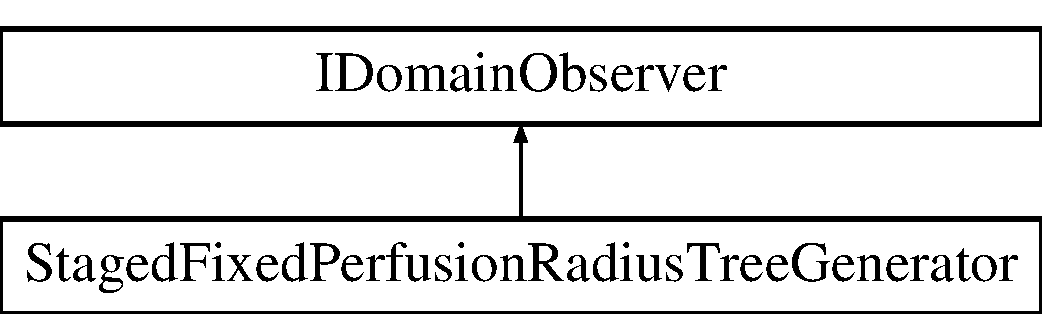
\includegraphics[height=2.000000cm]{d1/d25/class_staged_fixed_perfusion_radius_tree_generator}
\end{center}
\end{figure}
\subsection*{Public Member Functions}
\begin{DoxyCompactItemize}
\item 
\hyperlink{class_staged_fixed_perfusion_radius_tree_generator_a6ec7e6bccc6335836be4b43ae5f97f7b}{Staged\+Fixed\+Perfusion\+Radius\+Tree\+Generator} (\hyperlink{class_staged_domain}{Staged\+Domain} $\ast$\hyperlink{class_staged_fixed_perfusion_radius_tree_generator_a181b53d6b220d1b589f486c0a88d5c97}{domain}, \hyperlink{structpoint}{point} xi, double root\+Radii, double qi, long long int n\+Term, vector$<$ \hyperlink{class_abstract_constraint_function}{Abstract\+Constraint\+Function}$<$ double, int $>$ $\ast$ $>$gam, vector$<$ \hyperlink{class_abstract_constraint_function}{Abstract\+Constraint\+Function}$<$ double, int $>$ $\ast$ $>$eps\+Lim, vector$<$ \hyperlink{class_abstract_constraint_function}{Abstract\+Constraint\+Function}$<$ double, int $>$ $\ast$ $>$nu, double min\+Angle, double ref\+Pressure)
\item 
\hyperlink{class_staged_fixed_perfusion_radius_tree_generator_a116dcef71e28e75ca0bfe310a85aed31}{Staged\+Fixed\+Perfusion\+Radius\+Tree\+Generator} (\hyperlink{class_staged_domain}{Staged\+Domain} $\ast$\hyperlink{class_staged_fixed_perfusion_radius_tree_generator_a181b53d6b220d1b589f486c0a88d5c97}{domain}, \hyperlink{structpoint}{point} xi, double root\+Radii, double qi, long long int n\+Term, vector$<$ \hyperlink{class_abstract_constraint_function}{Abstract\+Constraint\+Function}$<$ double, int $>$ $\ast$ $>$gam, vector$<$ \hyperlink{class_abstract_constraint_function}{Abstract\+Constraint\+Function}$<$ double, int $>$ $\ast$ $>$eps\+Lim, vector$<$ \hyperlink{class_abstract_constraint_function}{Abstract\+Constraint\+Function}$<$ double, int $>$ $\ast$ $>$nu, double min\+Angle, double ref\+Pressure, double viscosity\+Tolerance, int optimized)
\item 
\hyperlink{class_staged_fixed_perfusion_radius_tree_generator_afde1c024b2fe7d34f8ad166838837885}{Staged\+Fixed\+Perfusion\+Radius\+Tree\+Generator} (\hyperlink{class_staged_domain}{Staged\+Domain} $\ast$\hyperlink{class_staged_fixed_perfusion_radius_tree_generator_a181b53d6b220d1b589f486c0a88d5c97}{domain}, \hyperlink{class_abstract_structured_c_c_o_tree}{Abstract\+Structured\+C\+C\+O\+Tree} $\ast$\hyperlink{class_staged_fixed_perfusion_radius_tree_generator_ae07119a1095859cc74c7144ea0b87040}{tree}, long long int n\+Term, vector$<$ \hyperlink{class_abstract_constraint_function}{Abstract\+Constraint\+Function}$<$ double, int $>$ $\ast$ $>$gam, vector$<$ \hyperlink{class_abstract_constraint_function}{Abstract\+Constraint\+Function}$<$ double, int $>$ $\ast$ $>$eps\+Lim, vector$<$ \hyperlink{class_abstract_constraint_function}{Abstract\+Constraint\+Function}$<$ double, int $>$ $\ast$ $>$nu)
\item 
\hyperlink{class_abstract_structured_c_c_o_tree}{Abstract\+Structured\+C\+C\+O\+Tree} $\ast$ \hyperlink{class_staged_fixed_perfusion_radius_tree_generator_a70ac52ecd809fe9a44a71837f7c2eba7}{generate} ()
\item 
\hyperlink{class_abstract_structured_c_c_o_tree}{Abstract\+Structured\+C\+C\+O\+Tree} $\ast$ \hyperlink{class_staged_fixed_perfusion_radius_tree_generator_a2090143d4271546bca00642d1c15047c}{resume} ()
\item 
\hyperlink{class_staged_domain}{Staged\+Domain} $\ast$ \hyperlink{class_staged_fixed_perfusion_radius_tree_generator_a961fc35b5a58d8c47127deb4214c53e6}{get\+Domain} ()
\item 
vector$<$ \hyperlink{class_abstract_structured_c_c_o_tree}{Abstract\+Structured\+C\+C\+O\+Tree} $\ast$ $>$ \hyperlink{class_staged_fixed_perfusion_radius_tree_generator_a11469cfa244770c9c79f8309238d8242}{get\+Trees} ()
\item 
void \hyperlink{class_staged_fixed_perfusion_radius_tree_generator_a7b086875be59a62a408934c8627dc07a}{enable\+Configuration\+File} (string filename)
\item 
void \hyperlink{class_staged_fixed_perfusion_radius_tree_generator_a344e071b8da2eea979efdbdeb650a2a6}{observable\+Modified} (\hyperlink{class_i_domain_observable}{I\+Domain\+Observable} $\ast$observable\+Instance)
\end{DoxyCompactItemize}
\subsection*{Protected Member Functions}
\begin{DoxyCompactItemize}
\item 
int \hyperlink{class_staged_fixed_perfusion_radius_tree_generator_ab8cfe2b17bc202e5cc7546ff9dc3d02b}{is\+Valid\+Root\+Segment} (\hyperlink{structpoint}{point} x\+New, int i\+Try)
\item 
int \hyperlink{class_staged_fixed_perfusion_radius_tree_generator_aecea1680252fab904014dddd59468b83}{is\+Valid\+Segment} (\hyperlink{structpoint}{point} x\+New, int i\+Try)
\item 
void \hyperlink{class_staged_fixed_perfusion_radius_tree_generator_ad520d182aaf13eef8ebf481a2b2a3087}{generates\+Configuration\+File} (ios\+::openmode mode)
\item 
void \hyperlink{class_staged_fixed_perfusion_radius_tree_generator_a58b8b5faaa3682b883376949f6741f0c}{mark\+Timestamp\+On\+Configuration\+File} (string label)
\item 
void \hyperlink{class_staged_fixed_perfusion_radius_tree_generator_a61d7acf210d76dd2d59fffc445c3b737}{close\+Configuration\+File} ()
\end{DoxyCompactItemize}
\subsection*{Protected Attributes}
\begin{DoxyCompactItemize}
\item 
ofstream \hyperlink{class_staged_fixed_perfusion_radius_tree_generator_a63c72bcaee798846d0dbc253faea577d}{conf\+File}
\item 
chrono\+::steady\+\_\+clock\+::time\+\_\+point \hyperlink{class_staged_fixed_perfusion_radius_tree_generator_abedb9de1a91a14d309a0119bb1bb48b8}{beginning\+Time}
\end{DoxyCompactItemize}
\subsection*{Private Attributes}
\begin{DoxyCompactItemize}
\item 
\hyperlink{class_generator_data}{Generator\+Data} $\ast$ \hyperlink{class_staged_fixed_perfusion_radius_tree_generator_a1b8f6b967274fe549955c6066f8836cc}{instance\+Data}
\item 
\hyperlink{class_generator_data_monitor}{Generator\+Data\+Monitor} $\ast$ \hyperlink{class_staged_fixed_perfusion_radius_tree_generator_ae1da125a5fc18e0622ed84ab1bb14c4d}{data\+Monitor}
\item 
long long int \hyperlink{class_staged_fixed_perfusion_radius_tree_generator_a2ae587dc32819ae4384fd095bc236511}{n\+Terminals}
\item 
double \hyperlink{class_staged_fixed_perfusion_radius_tree_generator_a24a92e7229dd55f85b14c6fa1a2fd648}{d\+Lim}
\item 
\hyperlink{class_staged_domain}{Staged\+Domain} $\ast$ \hyperlink{class_staged_fixed_perfusion_radius_tree_generator_a181b53d6b220d1b589f486c0a88d5c97}{domain}
\item 
\hyperlink{class_abstract_structured_c_c_o_tree}{Abstract\+Structured\+C\+C\+O\+Tree} $\ast$ \hyperlink{class_staged_fixed_perfusion_radius_tree_generator_ae07119a1095859cc74c7144ea0b87040}{tree}
\item 
vector$<$ \hyperlink{class_abstract_constraint_function}{Abstract\+Constraint\+Function}$<$ double, int $>$ $\ast$ $>$ {\bfseries gams}\hypertarget{class_staged_fixed_perfusion_radius_tree_generator_af6bb97cc854924f8df62faff70f1d015}{}\label{class_staged_fixed_perfusion_radius_tree_generator_af6bb97cc854924f8df62faff70f1d015}

\item 
vector$<$ \hyperlink{class_abstract_constraint_function}{Abstract\+Constraint\+Function}$<$ double, int $>$ $\ast$ $>$ {\bfseries eps\+Lims}\hypertarget{class_staged_fixed_perfusion_radius_tree_generator_a7a47d720671ae5b71d56ba8c5037a834}{}\label{class_staged_fixed_perfusion_radius_tree_generator_a7a47d720671ae5b71d56ba8c5037a834}

\item 
vector$<$ \hyperlink{class_abstract_constraint_function}{Abstract\+Constraint\+Function}$<$ double, int $>$ $\ast$ $>$ {\bfseries nus}\hypertarget{class_staged_fixed_perfusion_radius_tree_generator_aea533946c236a58fc9e850d268de6a0d}{}\label{class_staged_fixed_perfusion_radius_tree_generator_aea533946c236a58fc9e850d268de6a0d}

\item 
int {\bfseries stage}\hypertarget{class_staged_fixed_perfusion_radius_tree_generator_aa24f651f0a986011a43b6fe50eb334b5}{}\label{class_staged_fixed_perfusion_radius_tree_generator_aa24f651f0a986011a43b6fe50eb334b5}

\item 
int \hyperlink{class_staged_fixed_perfusion_radius_tree_generator_aeb2b61eca4e60b31209eb87730153db7}{is\+Generating\+Conf\+File}
\item 
string \hyperlink{class_staged_fixed_perfusion_radius_tree_generator_ab8dbc505effc0a2daf797f03741a8238}{conf\+Filename}
\end{DoxyCompactItemize}


\subsection{Detailed Description}
Generator for a single fixed perfusion tree with many stages. 

\subsection{Constructor \& Destructor Documentation}
\index{Staged\+Fixed\+Perfusion\+Radius\+Tree\+Generator@{Staged\+Fixed\+Perfusion\+Radius\+Tree\+Generator}!Staged\+Fixed\+Perfusion\+Radius\+Tree\+Generator@{Staged\+Fixed\+Perfusion\+Radius\+Tree\+Generator}}
\index{Staged\+Fixed\+Perfusion\+Radius\+Tree\+Generator@{Staged\+Fixed\+Perfusion\+Radius\+Tree\+Generator}!Staged\+Fixed\+Perfusion\+Radius\+Tree\+Generator@{Staged\+Fixed\+Perfusion\+Radius\+Tree\+Generator}}
\subsubsection[{\texorpdfstring{Staged\+Fixed\+Perfusion\+Radius\+Tree\+Generator(\+Staged\+Domain $\ast$domain, point xi, double root\+Radii, double qi, long long int n\+Term, vector$<$ Abstract\+Constraint\+Function$<$ double, int $>$ $\ast$ $>$gam, vector$<$ Abstract\+Constraint\+Function$<$ double, int $>$ $\ast$ $>$eps\+Lim, vector$<$ Abstract\+Constraint\+Function$<$ double, int $>$ $\ast$ $>$nu, double min\+Angle, double ref\+Pressure)}{StagedFixedPerfusionRadiusTreeGenerator(StagedDomain *domain, point xi, double rootRadii, double qi, long long int nTerm, vector< AbstractConstraintFunction< double, int > * >gam, vector< AbstractConstraintFunction< double, int > * >epsLim, vector< AbstractConstraintFunction< double, int > * >nu, double minAngle, double refPressure)}}]{\setlength{\rightskip}{0pt plus 5cm}Staged\+Fixed\+Perfusion\+Radius\+Tree\+Generator\+::\+Staged\+Fixed\+Perfusion\+Radius\+Tree\+Generator (
\begin{DoxyParamCaption}
\item[{{\bf Staged\+Domain} $\ast$}]{domain, }
\item[{{\bf point}}]{xi, }
\item[{double}]{root\+Radii, }
\item[{double}]{qi, }
\item[{long long int}]{n\+Term, }
\item[{vector$<$ {\bf Abstract\+Constraint\+Function}$<$ double, int $>$ $\ast$ $>$}]{gam, }
\item[{vector$<$ {\bf Abstract\+Constraint\+Function}$<$ double, int $>$ $\ast$ $>$}]{eps\+Lim, }
\item[{vector$<$ {\bf Abstract\+Constraint\+Function}$<$ double, int $>$ $\ast$ $>$}]{nu, }
\item[{double}]{min\+Angle, }
\item[{double}]{ref\+Pressure}
\end{DoxyParamCaption}
)}\hypertarget{class_staged_fixed_perfusion_radius_tree_generator_a6ec7e6bccc6335836be4b43ae5f97f7b}{}\label{class_staged_fixed_perfusion_radius_tree_generator_a6ec7e6bccc6335836be4b43ae5f97f7b}
Constructor for non-\/optimized and constant viscosity tree. 
\begin{DoxyParams}{Parameters}
{\em domain} & Perfusion domain. \\
\hline
{\em xi} & Root proximal position. \\
\hline
{\em root\+Radii} & Root radius. \\
\hline
{\em qi} & Inflow for the perfusion domain. \\
\hline
{\em n\+Term} & Total number of tree terminals. \\
\hline
{\em gam} & Murray\textquotesingle{}s power law function. \\
\hline
{\em eps\+Lim} & Symmetry constraint function. \\
\hline
{\em nu} & Viscosity function. \\
\hline
{\em min\+Angle} & Minimum allowed bifurcation angle. \\
\hline
\end{DoxyParams}
\index{Staged\+Fixed\+Perfusion\+Radius\+Tree\+Generator@{Staged\+Fixed\+Perfusion\+Radius\+Tree\+Generator}!Staged\+Fixed\+Perfusion\+Radius\+Tree\+Generator@{Staged\+Fixed\+Perfusion\+Radius\+Tree\+Generator}}
\index{Staged\+Fixed\+Perfusion\+Radius\+Tree\+Generator@{Staged\+Fixed\+Perfusion\+Radius\+Tree\+Generator}!Staged\+Fixed\+Perfusion\+Radius\+Tree\+Generator@{Staged\+Fixed\+Perfusion\+Radius\+Tree\+Generator}}
\subsubsection[{\texorpdfstring{Staged\+Fixed\+Perfusion\+Radius\+Tree\+Generator(\+Staged\+Domain $\ast$domain, point xi, double root\+Radii, double qi, long long int n\+Term, vector$<$ Abstract\+Constraint\+Function$<$ double, int $>$ $\ast$ $>$gam, vector$<$ Abstract\+Constraint\+Function$<$ double, int $>$ $\ast$ $>$eps\+Lim, vector$<$ Abstract\+Constraint\+Function$<$ double, int $>$ $\ast$ $>$nu, double min\+Angle, double ref\+Pressure, double viscosity\+Tolerance, int optimized)}{StagedFixedPerfusionRadiusTreeGenerator(StagedDomain *domain, point xi, double rootRadii, double qi, long long int nTerm, vector< AbstractConstraintFunction< double, int > * >gam, vector< AbstractConstraintFunction< double, int > * >epsLim, vector< AbstractConstraintFunction< double, int > * >nu, double minAngle, double refPressure, double viscosityTolerance, int optimized)}}]{\setlength{\rightskip}{0pt plus 5cm}Staged\+Fixed\+Perfusion\+Radius\+Tree\+Generator\+::\+Staged\+Fixed\+Perfusion\+Radius\+Tree\+Generator (
\begin{DoxyParamCaption}
\item[{{\bf Staged\+Domain} $\ast$}]{domain, }
\item[{{\bf point}}]{xi, }
\item[{double}]{root\+Radii, }
\item[{double}]{qi, }
\item[{long long int}]{n\+Term, }
\item[{vector$<$ {\bf Abstract\+Constraint\+Function}$<$ double, int $>$ $\ast$ $>$}]{gam, }
\item[{vector$<$ {\bf Abstract\+Constraint\+Function}$<$ double, int $>$ $\ast$ $>$}]{eps\+Lim, }
\item[{vector$<$ {\bf Abstract\+Constraint\+Function}$<$ double, int $>$ $\ast$ $>$}]{nu, }
\item[{double}]{min\+Angle, }
\item[{double}]{ref\+Pressure, }
\item[{double}]{viscosity\+Tolerance, }
\item[{int}]{optimized}
\end{DoxyParamCaption}
)}\hypertarget{class_staged_fixed_perfusion_radius_tree_generator_a116dcef71e28e75ca0bfe310a85aed31}{}\label{class_staged_fixed_perfusion_radius_tree_generator_a116dcef71e28e75ca0bfe310a85aed31}
Constructor for tree with Fahraeus-\/\+Lindquist viscosity model. 
\begin{DoxyParams}{Parameters}
{\em domain} & Perfusion domain. \\
\hline
{\em xi} & Root proximal position. \\
\hline
{\em root\+Radii} & Root radius. \\
\hline
{\em qi} & Inflow for the perfusion domain. \\
\hline
{\em n\+Term} & Total number of tree terminals. \\
\hline
{\em gam} & Murray\textquotesingle{}s power law function. \\
\hline
{\em eps\+Lim} & Symmetry constraint function. \\
\hline
{\em nu} & Viscosity function. \\
\hline
{\em min\+Angle} & Minimum allowed bifurcation angle. \\
\hline
{\em viscosity\+Tolerance} & Convergence tolerance for the absolute beta variation in the viscosity iterative scheme. \\
\hline
{\em optimized} & If it is optimized with partial tree scaling. \\
\hline
\end{DoxyParams}
\index{Staged\+Fixed\+Perfusion\+Radius\+Tree\+Generator@{Staged\+Fixed\+Perfusion\+Radius\+Tree\+Generator}!Staged\+Fixed\+Perfusion\+Radius\+Tree\+Generator@{Staged\+Fixed\+Perfusion\+Radius\+Tree\+Generator}}
\index{Staged\+Fixed\+Perfusion\+Radius\+Tree\+Generator@{Staged\+Fixed\+Perfusion\+Radius\+Tree\+Generator}!Staged\+Fixed\+Perfusion\+Radius\+Tree\+Generator@{Staged\+Fixed\+Perfusion\+Radius\+Tree\+Generator}}
\subsubsection[{\texorpdfstring{Staged\+Fixed\+Perfusion\+Radius\+Tree\+Generator(\+Staged\+Domain $\ast$domain, Abstract\+Structured\+C\+C\+O\+Tree $\ast$tree, long long int n\+Term, vector$<$ Abstract\+Constraint\+Function$<$ double, int $>$ $\ast$ $>$gam, vector$<$ Abstract\+Constraint\+Function$<$ double, int $>$ $\ast$ $>$eps\+Lim, vector$<$ Abstract\+Constraint\+Function$<$ double, int $>$ $\ast$ $>$nu)}{StagedFixedPerfusionRadiusTreeGenerator(StagedDomain *domain, AbstractStructuredCCOTree *tree, long long int nTerm, vector< AbstractConstraintFunction< double, int > * >gam, vector< AbstractConstraintFunction< double, int > * >epsLim, vector< AbstractConstraintFunction< double, int > * >nu)}}]{\setlength{\rightskip}{0pt plus 5cm}Staged\+Fixed\+Perfusion\+Radius\+Tree\+Generator\+::\+Staged\+Fixed\+Perfusion\+Radius\+Tree\+Generator (
\begin{DoxyParamCaption}
\item[{{\bf Staged\+Domain} $\ast$}]{domain, }
\item[{{\bf Abstract\+Structured\+C\+C\+O\+Tree} $\ast$}]{tree, }
\item[{long long int}]{n\+Term, }
\item[{vector$<$ {\bf Abstract\+Constraint\+Function}$<$ double, int $>$ $\ast$ $>$}]{gam, }
\item[{vector$<$ {\bf Abstract\+Constraint\+Function}$<$ double, int $>$ $\ast$ $>$}]{eps\+Lim, }
\item[{vector$<$ {\bf Abstract\+Constraint\+Function}$<$ double, int $>$ $\ast$ $>$}]{nu}
\end{DoxyParamCaption}
)}\hypertarget{class_staged_fixed_perfusion_radius_tree_generator_afde1c024b2fe7d34f8ad166838837885}{}\label{class_staged_fixed_perfusion_radius_tree_generator_afde1c024b2fe7d34f8ad166838837885}
Constructor to resume from a pre-\/existent tree. 
\begin{DoxyParams}{Parameters}
{\em domain} & Perfusion domain. \\
\hline
{\em tree} & Pre-\/existent tree. \\
\hline
{\em n\+Term} & Total number of tree terminals. \\
\hline
{\em gam} & Murray\textquotesingle{}s power law function. \\
\hline
{\em eps\+Lim} & Symmetry constraint function. \\
\hline
{\em nu} & Viscosity function. \\
\hline
\end{DoxyParams}


\subsection{Member Function Documentation}
\index{Staged\+Fixed\+Perfusion\+Radius\+Tree\+Generator@{Staged\+Fixed\+Perfusion\+Radius\+Tree\+Generator}!close\+Configuration\+File@{close\+Configuration\+File}}
\index{close\+Configuration\+File@{close\+Configuration\+File}!Staged\+Fixed\+Perfusion\+Radius\+Tree\+Generator@{Staged\+Fixed\+Perfusion\+Radius\+Tree\+Generator}}
\subsubsection[{\texorpdfstring{close\+Configuration\+File()}{closeConfigurationFile()}}]{\setlength{\rightskip}{0pt plus 5cm}void Staged\+Fixed\+Perfusion\+Radius\+Tree\+Generator\+::close\+Configuration\+File (
\begin{DoxyParamCaption}
{}
\end{DoxyParamCaption}
)\hspace{0.3cm}{\ttfamily [protected]}}\hypertarget{class_staged_fixed_perfusion_radius_tree_generator_a61d7acf210d76dd2d59fffc445c3b737}{}\label{class_staged_fixed_perfusion_radius_tree_generator_a61d7acf210d76dd2d59fffc445c3b737}
Closes the configuration file for the current tree generation. \index{Staged\+Fixed\+Perfusion\+Radius\+Tree\+Generator@{Staged\+Fixed\+Perfusion\+Radius\+Tree\+Generator}!enable\+Configuration\+File@{enable\+Configuration\+File}}
\index{enable\+Configuration\+File@{enable\+Configuration\+File}!Staged\+Fixed\+Perfusion\+Radius\+Tree\+Generator@{Staged\+Fixed\+Perfusion\+Radius\+Tree\+Generator}}
\subsubsection[{\texorpdfstring{enable\+Configuration\+File(string filename)}{enableConfigurationFile(string filename)}}]{\setlength{\rightskip}{0pt plus 5cm}void Staged\+Fixed\+Perfusion\+Radius\+Tree\+Generator\+::enable\+Configuration\+File (
\begin{DoxyParamCaption}
\item[{string}]{filename}
\end{DoxyParamCaption}
)}\hypertarget{class_staged_fixed_perfusion_radius_tree_generator_a7b086875be59a62a408934c8627dc07a}{}\label{class_staged_fixed_perfusion_radius_tree_generator_a7b086875be59a62a408934c8627dc07a}
Enables the configuration file generation capabilities. 
\begin{DoxyParams}{Parameters}
{\em filename} & File name where the generator stores the configuration data. \\
\hline
\end{DoxyParams}
\index{Staged\+Fixed\+Perfusion\+Radius\+Tree\+Generator@{Staged\+Fixed\+Perfusion\+Radius\+Tree\+Generator}!generate@{generate}}
\index{generate@{generate}!Staged\+Fixed\+Perfusion\+Radius\+Tree\+Generator@{Staged\+Fixed\+Perfusion\+Radius\+Tree\+Generator}}
\subsubsection[{\texorpdfstring{generate()}{generate()}}]{\setlength{\rightskip}{0pt plus 5cm}{\bf Abstract\+Structured\+C\+C\+O\+Tree} $\ast$ Staged\+Fixed\+Perfusion\+Radius\+Tree\+Generator\+::generate (
\begin{DoxyParamCaption}
{}
\end{DoxyParamCaption}
)}\hypertarget{class_staged_fixed_perfusion_radius_tree_generator_a70ac52ecd809fe9a44a71837f7c2eba7}{}\label{class_staged_fixed_perfusion_radius_tree_generator_a70ac52ecd809fe9a44a71837f7c2eba7}
Generates the specified tree. \begin{DoxyReturn}{Returns}
Perfusion tree. 
\end{DoxyReturn}
\index{Staged\+Fixed\+Perfusion\+Radius\+Tree\+Generator@{Staged\+Fixed\+Perfusion\+Radius\+Tree\+Generator}!generates\+Configuration\+File@{generates\+Configuration\+File}}
\index{generates\+Configuration\+File@{generates\+Configuration\+File}!Staged\+Fixed\+Perfusion\+Radius\+Tree\+Generator@{Staged\+Fixed\+Perfusion\+Radius\+Tree\+Generator}}
\subsubsection[{\texorpdfstring{generates\+Configuration\+File(ios\+::openmode mode)}{generatesConfigurationFile(ios::openmode mode)}}]{\setlength{\rightskip}{0pt plus 5cm}void Staged\+Fixed\+Perfusion\+Radius\+Tree\+Generator\+::generates\+Configuration\+File (
\begin{DoxyParamCaption}
\item[{ios\+::openmode}]{mode}
\end{DoxyParamCaption}
)\hspace{0.3cm}{\ttfamily [protected]}}\hypertarget{class_staged_fixed_perfusion_radius_tree_generator_ad520d182aaf13eef8ebf481a2b2a3087}{}\label{class_staged_fixed_perfusion_radius_tree_generator_ad520d182aaf13eef8ebf481a2b2a3087}
Generates the configuration file for the current tree generation. 
\begin{DoxyParams}{Parameters}
{\em mode} & Is the openmode used for the generated file (ios\+::out for generation, ios\+::app for resume). \\
\hline
\end{DoxyParams}
\index{Staged\+Fixed\+Perfusion\+Radius\+Tree\+Generator@{Staged\+Fixed\+Perfusion\+Radius\+Tree\+Generator}!get\+Domain@{get\+Domain}}
\index{get\+Domain@{get\+Domain}!Staged\+Fixed\+Perfusion\+Radius\+Tree\+Generator@{Staged\+Fixed\+Perfusion\+Radius\+Tree\+Generator}}
\subsubsection[{\texorpdfstring{get\+Domain()}{getDomain()}}]{\setlength{\rightskip}{0pt plus 5cm}{\bf Staged\+Domain} $\ast$ Staged\+Fixed\+Perfusion\+Radius\+Tree\+Generator\+::get\+Domain (
\begin{DoxyParamCaption}
{}
\end{DoxyParamCaption}
)}\hypertarget{class_staged_fixed_perfusion_radius_tree_generator_a961fc35b5a58d8c47127deb4214c53e6}{}\label{class_staged_fixed_perfusion_radius_tree_generator_a961fc35b5a58d8c47127deb4214c53e6}
Returns the perfusion domain. \begin{DoxyReturn}{Returns}
Perfusion domain. 
\end{DoxyReturn}
\index{Staged\+Fixed\+Perfusion\+Radius\+Tree\+Generator@{Staged\+Fixed\+Perfusion\+Radius\+Tree\+Generator}!get\+Trees@{get\+Trees}}
\index{get\+Trees@{get\+Trees}!Staged\+Fixed\+Perfusion\+Radius\+Tree\+Generator@{Staged\+Fixed\+Perfusion\+Radius\+Tree\+Generator}}
\subsubsection[{\texorpdfstring{get\+Trees()}{getTrees()}}]{\setlength{\rightskip}{0pt plus 5cm}vector$<$ {\bf Abstract\+Structured\+C\+C\+O\+Tree} $\ast$ $>$ Staged\+Fixed\+Perfusion\+Radius\+Tree\+Generator\+::get\+Trees (
\begin{DoxyParamCaption}
{}
\end{DoxyParamCaption}
)}\hypertarget{class_staged_fixed_perfusion_radius_tree_generator_a11469cfa244770c9c79f8309238d8242}{}\label{class_staged_fixed_perfusion_radius_tree_generator_a11469cfa244770c9c79f8309238d8242}
Returns the generated tree. \begin{DoxyReturn}{Returns}
Generated tree. 
\end{DoxyReturn}
\index{Staged\+Fixed\+Perfusion\+Radius\+Tree\+Generator@{Staged\+Fixed\+Perfusion\+Radius\+Tree\+Generator}!is\+Valid\+Root\+Segment@{is\+Valid\+Root\+Segment}}
\index{is\+Valid\+Root\+Segment@{is\+Valid\+Root\+Segment}!Staged\+Fixed\+Perfusion\+Radius\+Tree\+Generator@{Staged\+Fixed\+Perfusion\+Radius\+Tree\+Generator}}
\subsubsection[{\texorpdfstring{is\+Valid\+Root\+Segment(point x\+New, int i\+Try)}{isValidRootSegment(point xNew, int iTry)}}]{\setlength{\rightskip}{0pt plus 5cm}int Staged\+Fixed\+Perfusion\+Radius\+Tree\+Generator\+::is\+Valid\+Root\+Segment (
\begin{DoxyParamCaption}
\item[{{\bf point}}]{x\+New, }
\item[{int}]{i\+Try}
\end{DoxyParamCaption}
)\hspace{0.3cm}{\ttfamily [protected]}}\hypertarget{class_staged_fixed_perfusion_radius_tree_generator_ab8cfe2b17bc202e5cc7546ff9dc3d02b}{}\label{class_staged_fixed_perfusion_radius_tree_generator_ab8cfe2b17bc202e5cc7546ff9dc3d02b}
Returns if the length of the segment defined by x\+Prox and x\+New is higher than d\+Lim (distance criterion). 
\begin{DoxyParams}{Parameters}
{\em x\+New} & Proposed distal point. \\
\hline
{\em i\+Try} & Number of trial. \\
\hline
\end{DoxyParams}
\begin{DoxyReturn}{Returns}
If the root segment is valid. 
\end{DoxyReturn}
\index{Staged\+Fixed\+Perfusion\+Radius\+Tree\+Generator@{Staged\+Fixed\+Perfusion\+Radius\+Tree\+Generator}!is\+Valid\+Segment@{is\+Valid\+Segment}}
\index{is\+Valid\+Segment@{is\+Valid\+Segment}!Staged\+Fixed\+Perfusion\+Radius\+Tree\+Generator@{Staged\+Fixed\+Perfusion\+Radius\+Tree\+Generator}}
\subsubsection[{\texorpdfstring{is\+Valid\+Segment(point x\+New, int i\+Try)}{isValidSegment(point xNew, int iTry)}}]{\setlength{\rightskip}{0pt plus 5cm}int Staged\+Fixed\+Perfusion\+Radius\+Tree\+Generator\+::is\+Valid\+Segment (
\begin{DoxyParamCaption}
\item[{{\bf point}}]{x\+New, }
\item[{int}]{i\+Try}
\end{DoxyParamCaption}
)\hspace{0.3cm}{\ttfamily [protected]}}\hypertarget{class_staged_fixed_perfusion_radius_tree_generator_aecea1680252fab904014dddd59468b83}{}\label{class_staged_fixed_perfusion_radius_tree_generator_aecea1680252fab904014dddd59468b83}
Returns if the closest point to the whole try is greater than d\+Lim (distance criterion for a new segment). 
\begin{DoxyParams}{Parameters}
{\em x\+New} & Proposed distal point. \\
\hline
{\em i\+Try} & Number of trial. \\
\hline
\end{DoxyParams}
\begin{DoxyReturn}{Returns}
If the segment is valid. 
\end{DoxyReturn}
\index{Staged\+Fixed\+Perfusion\+Radius\+Tree\+Generator@{Staged\+Fixed\+Perfusion\+Radius\+Tree\+Generator}!mark\+Timestamp\+On\+Configuration\+File@{mark\+Timestamp\+On\+Configuration\+File}}
\index{mark\+Timestamp\+On\+Configuration\+File@{mark\+Timestamp\+On\+Configuration\+File}!Staged\+Fixed\+Perfusion\+Radius\+Tree\+Generator@{Staged\+Fixed\+Perfusion\+Radius\+Tree\+Generator}}
\subsubsection[{\texorpdfstring{mark\+Timestamp\+On\+Configuration\+File(string label)}{markTimestampOnConfigurationFile(string label)}}]{\setlength{\rightskip}{0pt plus 5cm}void Staged\+Fixed\+Perfusion\+Radius\+Tree\+Generator\+::mark\+Timestamp\+On\+Configuration\+File (
\begin{DoxyParamCaption}
\item[{string}]{label}
\end{DoxyParamCaption}
)\hspace{0.3cm}{\ttfamily [protected]}}\hypertarget{class_staged_fixed_perfusion_radius_tree_generator_a58b8b5faaa3682b883376949f6741f0c}{}\label{class_staged_fixed_perfusion_radius_tree_generator_a58b8b5faaa3682b883376949f6741f0c}
Saves the timestamp for event {\ttfamily label}. \index{Staged\+Fixed\+Perfusion\+Radius\+Tree\+Generator@{Staged\+Fixed\+Perfusion\+Radius\+Tree\+Generator}!observable\+Modified@{observable\+Modified}}
\index{observable\+Modified@{observable\+Modified}!Staged\+Fixed\+Perfusion\+Radius\+Tree\+Generator@{Staged\+Fixed\+Perfusion\+Radius\+Tree\+Generator}}
\subsubsection[{\texorpdfstring{observable\+Modified(\+I\+Domain\+Observable $\ast$observable\+Instance)}{observableModified(IDomainObservable *observableInstance)}}]{\setlength{\rightskip}{0pt plus 5cm}void Staged\+Fixed\+Perfusion\+Radius\+Tree\+Generator\+::observable\+Modified (
\begin{DoxyParamCaption}
\item[{{\bf I\+Domain\+Observable} $\ast$}]{observable\+Instance}
\end{DoxyParamCaption}
)\hspace{0.3cm}{\ttfamily [virtual]}}\hypertarget{class_staged_fixed_perfusion_radius_tree_generator_a344e071b8da2eea979efdbdeb650a2a6}{}\label{class_staged_fixed_perfusion_radius_tree_generator_a344e071b8da2eea979efdbdeb650a2a6}
Updates internal data from this instance after the domain has been modified. 
\begin{DoxyParams}{Parameters}
{\em observable\+Instance} & Domain instance modified. \\
\hline
\end{DoxyParams}


Implements \hyperlink{class_i_domain_observer_aee18640c20a6feaa16e4bf3bdde887a3}{I\+Domain\+Observer}.

\index{Staged\+Fixed\+Perfusion\+Radius\+Tree\+Generator@{Staged\+Fixed\+Perfusion\+Radius\+Tree\+Generator}!resume@{resume}}
\index{resume@{resume}!Staged\+Fixed\+Perfusion\+Radius\+Tree\+Generator@{Staged\+Fixed\+Perfusion\+Radius\+Tree\+Generator}}
\subsubsection[{\texorpdfstring{resume()}{resume()}}]{\setlength{\rightskip}{0pt plus 5cm}{\bf Abstract\+Structured\+C\+C\+O\+Tree} $\ast$ Staged\+Fixed\+Perfusion\+Radius\+Tree\+Generator\+::resume (
\begin{DoxyParamCaption}
{}
\end{DoxyParamCaption}
)}\hypertarget{class_staged_fixed_perfusion_radius_tree_generator_a2090143d4271546bca00642d1c15047c}{}\label{class_staged_fixed_perfusion_radius_tree_generator_a2090143d4271546bca00642d1c15047c}
Resumes the tree generation. \begin{DoxyReturn}{Returns}
Perfusion tree. 
\end{DoxyReturn}


\subsection{Member Data Documentation}
\index{Staged\+Fixed\+Perfusion\+Radius\+Tree\+Generator@{Staged\+Fixed\+Perfusion\+Radius\+Tree\+Generator}!beginning\+Time@{beginning\+Time}}
\index{beginning\+Time@{beginning\+Time}!Staged\+Fixed\+Perfusion\+Radius\+Tree\+Generator@{Staged\+Fixed\+Perfusion\+Radius\+Tree\+Generator}}
\subsubsection[{\texorpdfstring{beginning\+Time}{beginningTime}}]{\setlength{\rightskip}{0pt plus 5cm}chrono\+::steady\+\_\+clock\+::time\+\_\+point Staged\+Fixed\+Perfusion\+Radius\+Tree\+Generator\+::beginning\+Time\hspace{0.3cm}{\ttfamily [protected]}}\hypertarget{class_staged_fixed_perfusion_radius_tree_generator_abedb9de1a91a14d309a0119bb1bb48b8}{}\label{class_staged_fixed_perfusion_radius_tree_generator_abedb9de1a91a14d309a0119bb1bb48b8}
Initial timestamp of the generation process. \index{Staged\+Fixed\+Perfusion\+Radius\+Tree\+Generator@{Staged\+Fixed\+Perfusion\+Radius\+Tree\+Generator}!conf\+File@{conf\+File}}
\index{conf\+File@{conf\+File}!Staged\+Fixed\+Perfusion\+Radius\+Tree\+Generator@{Staged\+Fixed\+Perfusion\+Radius\+Tree\+Generator}}
\subsubsection[{\texorpdfstring{conf\+File}{confFile}}]{\setlength{\rightskip}{0pt plus 5cm}ofstream Staged\+Fixed\+Perfusion\+Radius\+Tree\+Generator\+::conf\+File\hspace{0.3cm}{\ttfamily [protected]}}\hypertarget{class_staged_fixed_perfusion_radius_tree_generator_a63c72bcaee798846d0dbc253faea577d}{}\label{class_staged_fixed_perfusion_radius_tree_generator_a63c72bcaee798846d0dbc253faea577d}
Configuration file stream. \index{Staged\+Fixed\+Perfusion\+Radius\+Tree\+Generator@{Staged\+Fixed\+Perfusion\+Radius\+Tree\+Generator}!conf\+Filename@{conf\+Filename}}
\index{conf\+Filename@{conf\+Filename}!Staged\+Fixed\+Perfusion\+Radius\+Tree\+Generator@{Staged\+Fixed\+Perfusion\+Radius\+Tree\+Generator}}
\subsubsection[{\texorpdfstring{conf\+Filename}{confFilename}}]{\setlength{\rightskip}{0pt plus 5cm}string Staged\+Fixed\+Perfusion\+Radius\+Tree\+Generator\+::conf\+Filename\hspace{0.3cm}{\ttfamily [private]}}\hypertarget{class_staged_fixed_perfusion_radius_tree_generator_ab8dbc505effc0a2daf797f03741a8238}{}\label{class_staged_fixed_perfusion_radius_tree_generator_ab8dbc505effc0a2daf797f03741a8238}
File name for the configuration file. \index{Staged\+Fixed\+Perfusion\+Radius\+Tree\+Generator@{Staged\+Fixed\+Perfusion\+Radius\+Tree\+Generator}!data\+Monitor@{data\+Monitor}}
\index{data\+Monitor@{data\+Monitor}!Staged\+Fixed\+Perfusion\+Radius\+Tree\+Generator@{Staged\+Fixed\+Perfusion\+Radius\+Tree\+Generator}}
\subsubsection[{\texorpdfstring{data\+Monitor}{dataMonitor}}]{\setlength{\rightskip}{0pt plus 5cm}{\bf Generator\+Data\+Monitor}$\ast$ Staged\+Fixed\+Perfusion\+Radius\+Tree\+Generator\+::data\+Monitor\hspace{0.3cm}{\ttfamily [private]}}\hypertarget{class_staged_fixed_perfusion_radius_tree_generator_ae1da125a5fc18e0622ed84ab1bb14c4d}{}\label{class_staged_fixed_perfusion_radius_tree_generator_ae1da125a5fc18e0622ed84ab1bb14c4d}
Monitor of the {\ttfamily instance\+Data} . \index{Staged\+Fixed\+Perfusion\+Radius\+Tree\+Generator@{Staged\+Fixed\+Perfusion\+Radius\+Tree\+Generator}!d\+Lim@{d\+Lim}}
\index{d\+Lim@{d\+Lim}!Staged\+Fixed\+Perfusion\+Radius\+Tree\+Generator@{Staged\+Fixed\+Perfusion\+Radius\+Tree\+Generator}}
\subsubsection[{\texorpdfstring{d\+Lim}{dLim}}]{\setlength{\rightskip}{0pt plus 5cm}double Staged\+Fixed\+Perfusion\+Radius\+Tree\+Generator\+::d\+Lim\hspace{0.3cm}{\ttfamily [private]}}\hypertarget{class_staged_fixed_perfusion_radius_tree_generator_a24a92e7229dd55f85b14c6fa1a2fd648}{}\label{class_staged_fixed_perfusion_radius_tree_generator_a24a92e7229dd55f85b14c6fa1a2fd648}
Perfusion volume. \index{Staged\+Fixed\+Perfusion\+Radius\+Tree\+Generator@{Staged\+Fixed\+Perfusion\+Radius\+Tree\+Generator}!domain@{domain}}
\index{domain@{domain}!Staged\+Fixed\+Perfusion\+Radius\+Tree\+Generator@{Staged\+Fixed\+Perfusion\+Radius\+Tree\+Generator}}
\subsubsection[{\texorpdfstring{domain}{domain}}]{\setlength{\rightskip}{0pt plus 5cm}{\bf Staged\+Domain}$\ast$ Staged\+Fixed\+Perfusion\+Radius\+Tree\+Generator\+::domain\hspace{0.3cm}{\ttfamily [private]}}\hypertarget{class_staged_fixed_perfusion_radius_tree_generator_a181b53d6b220d1b589f486c0a88d5c97}{}\label{class_staged_fixed_perfusion_radius_tree_generator_a181b53d6b220d1b589f486c0a88d5c97}
Perfusion domain. \index{Staged\+Fixed\+Perfusion\+Radius\+Tree\+Generator@{Staged\+Fixed\+Perfusion\+Radius\+Tree\+Generator}!instance\+Data@{instance\+Data}}
\index{instance\+Data@{instance\+Data}!Staged\+Fixed\+Perfusion\+Radius\+Tree\+Generator@{Staged\+Fixed\+Perfusion\+Radius\+Tree\+Generator}}
\subsubsection[{\texorpdfstring{instance\+Data}{instanceData}}]{\setlength{\rightskip}{0pt plus 5cm}{\bf Generator\+Data}$\ast$ Staged\+Fixed\+Perfusion\+Radius\+Tree\+Generator\+::instance\+Data\hspace{0.3cm}{\ttfamily [private]}}\hypertarget{class_staged_fixed_perfusion_radius_tree_generator_a1b8f6b967274fe549955c6066f8836cc}{}\label{class_staged_fixed_perfusion_radius_tree_generator_a1b8f6b967274fe549955c6066f8836cc}
Wrapper with parameters associated to a tree generation process. \index{Staged\+Fixed\+Perfusion\+Radius\+Tree\+Generator@{Staged\+Fixed\+Perfusion\+Radius\+Tree\+Generator}!is\+Generating\+Conf\+File@{is\+Generating\+Conf\+File}}
\index{is\+Generating\+Conf\+File@{is\+Generating\+Conf\+File}!Staged\+Fixed\+Perfusion\+Radius\+Tree\+Generator@{Staged\+Fixed\+Perfusion\+Radius\+Tree\+Generator}}
\subsubsection[{\texorpdfstring{is\+Generating\+Conf\+File}{isGeneratingConfFile}}]{\setlength{\rightskip}{0pt plus 5cm}int Staged\+Fixed\+Perfusion\+Radius\+Tree\+Generator\+::is\+Generating\+Conf\+File\hspace{0.3cm}{\ttfamily [private]}}\hypertarget{class_staged_fixed_perfusion_radius_tree_generator_aeb2b61eca4e60b31209eb87730153db7}{}\label{class_staged_fixed_perfusion_radius_tree_generator_aeb2b61eca4e60b31209eb87730153db7}
If the current generation saves the configuration used. \index{Staged\+Fixed\+Perfusion\+Radius\+Tree\+Generator@{Staged\+Fixed\+Perfusion\+Radius\+Tree\+Generator}!n\+Terminals@{n\+Terminals}}
\index{n\+Terminals@{n\+Terminals}!Staged\+Fixed\+Perfusion\+Radius\+Tree\+Generator@{Staged\+Fixed\+Perfusion\+Radius\+Tree\+Generator}}
\subsubsection[{\texorpdfstring{n\+Terminals}{nTerminals}}]{\setlength{\rightskip}{0pt plus 5cm}long long int Staged\+Fixed\+Perfusion\+Radius\+Tree\+Generator\+::n\+Terminals\hspace{0.3cm}{\ttfamily [private]}}\hypertarget{class_staged_fixed_perfusion_radius_tree_generator_a2ae587dc32819ae4384fd095bc236511}{}\label{class_staged_fixed_perfusion_radius_tree_generator_a2ae587dc32819ae4384fd095bc236511}
Amount of terminals in the trees. \index{Staged\+Fixed\+Perfusion\+Radius\+Tree\+Generator@{Staged\+Fixed\+Perfusion\+Radius\+Tree\+Generator}!tree@{tree}}
\index{tree@{tree}!Staged\+Fixed\+Perfusion\+Radius\+Tree\+Generator@{Staged\+Fixed\+Perfusion\+Radius\+Tree\+Generator}}
\subsubsection[{\texorpdfstring{tree}{tree}}]{\setlength{\rightskip}{0pt plus 5cm}{\bf Abstract\+Structured\+C\+C\+O\+Tree}$\ast$ Staged\+Fixed\+Perfusion\+Radius\+Tree\+Generator\+::tree\hspace{0.3cm}{\ttfamily [private]}}\hypertarget{class_staged_fixed_perfusion_radius_tree_generator_ae07119a1095859cc74c7144ea0b87040}{}\label{class_staged_fixed_perfusion_radius_tree_generator_ae07119a1095859cc74c7144ea0b87040}
Generated trees. 

The documentation for this class was generated from the following files\+:\begin{DoxyCompactItemize}
\item 
core/Staged\+Fixed\+Perfusion\+Radius\+Tree\+Generator.\+h\item 
core/Staged\+Fixed\+Perfusion\+Radius\+Tree\+Generator.\+cpp\end{DoxyCompactItemize}

\hypertarget{class_staged_f_r_r_o_tree_generator}{}\section{Staged\+F\+R\+R\+O\+Tree\+Generator Class Reference}
\label{class_staged_f_r_r_o_tree_generator}\index{Staged\+F\+R\+R\+O\+Tree\+Generator@{Staged\+F\+R\+R\+O\+Tree\+Generator}}


{\ttfamily \#include $<$Staged\+F\+R\+R\+O\+Tree\+Generator.\+h$>$}

Inheritance diagram for Staged\+F\+R\+R\+O\+Tree\+Generator\+:\begin{figure}[H]
\begin{center}
\leavevmode
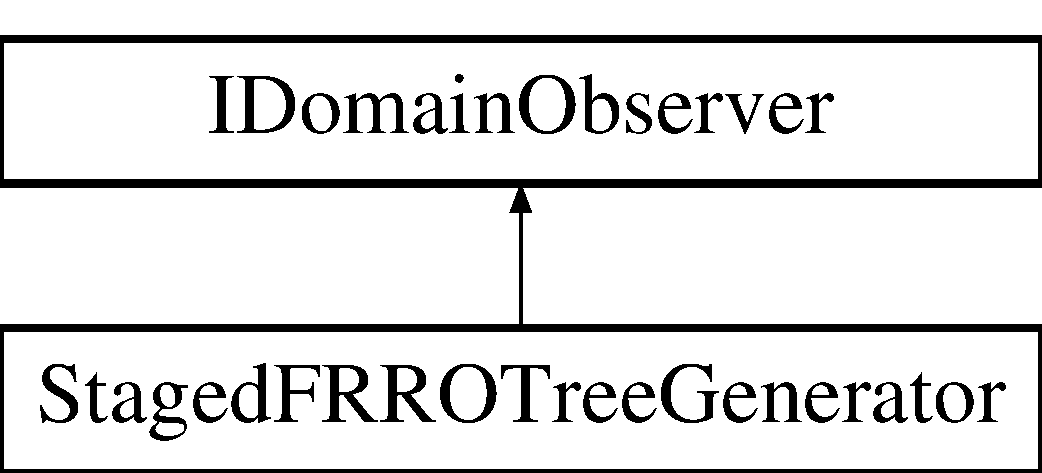
\includegraphics[height=2.000000cm]{d5/dd5/class_staged_f_r_r_o_tree_generator}
\end{center}
\end{figure}
\subsection*{Public Member Functions}
\begin{DoxyCompactItemize}
\item 
\hyperlink{class_staged_f_r_r_o_tree_generator_a00f41805e256a579e91c4519fab7b016}{Staged\+F\+R\+R\+O\+Tree\+Generator} (\hyperlink{class_staged_domain}{Staged\+Domain} $\ast$\hyperlink{class_staged_f_r_r_o_tree_generator_a2f8616a24551a7a414b51b805309894a}{domain}, \hyperlink{structpoint}{point} xi, double root\+Radii, double qi, long long int n\+Term, vector$<$ \hyperlink{class_abstract_constraint_function}{Abstract\+Constraint\+Function}$<$ double, int $>$ $\ast$ $>$gam, vector$<$ \hyperlink{class_abstract_constraint_function}{Abstract\+Constraint\+Function}$<$ double, int $>$ $\ast$ $>$eps\+Lim, vector$<$ \hyperlink{class_abstract_constraint_function}{Abstract\+Constraint\+Function}$<$ double, int $>$ $\ast$ $>$nu, double min\+Angle, double ref\+Pressure, double viscosity\+Tolerance)
\item 
\hyperlink{class_staged_f_r_r_o_tree_generator_a3dc2c3e1959e0df5d1a46c696acdcf0a}{Staged\+F\+R\+R\+O\+Tree\+Generator} (\hyperlink{class_staged_domain}{Staged\+Domain} $\ast$\hyperlink{class_staged_f_r_r_o_tree_generator_a2f8616a24551a7a414b51b805309894a}{domain}, \hyperlink{class_abstract_object_c_c_o_tree}{Abstract\+Object\+C\+C\+O\+Tree} $\ast$\hyperlink{class_staged_f_r_r_o_tree_generator_a3d7a0b0194b93d4c2706a21908ad9f09}{tree}, long long int n\+Term, vector$<$ \hyperlink{class_abstract_constraint_function}{Abstract\+Constraint\+Function}$<$ double, int $>$ $\ast$ $>$gam, vector$<$ \hyperlink{class_abstract_constraint_function}{Abstract\+Constraint\+Function}$<$ double, int $>$ $\ast$ $>$eps\+Lim, vector$<$ \hyperlink{class_abstract_constraint_function}{Abstract\+Constraint\+Function}$<$ double, int $>$ $\ast$ $>$nu)
\item 
\hyperlink{class_staged_f_r_r_o_tree_generator_ace0cc12588d7ca428520e5e08dfd5e83}{$\sim$\+Staged\+F\+R\+R\+O\+Tree\+Generator} ()
\item 
\hyperlink{class_abstract_object_c_c_o_tree}{Abstract\+Object\+C\+C\+O\+Tree} $\ast$ \hyperlink{class_staged_f_r_r_o_tree_generator_acdd7fefb4e091a21f870e305da66e4e1}{generate} (long long int save\+Interval)
\item 
\hyperlink{class_abstract_object_c_c_o_tree}{Abstract\+Object\+C\+C\+O\+Tree} $\ast$ \hyperlink{class_staged_f_r_r_o_tree_generator_a32d59d858cf3859dc0ed4db13f2a8642}{resume} (long long int save\+Interval)
\item 
\hyperlink{class_staged_domain}{Staged\+Domain} $\ast$ \hyperlink{class_staged_f_r_r_o_tree_generator_adac14b11b09b21df02d635ed124216a7}{get\+Domain} ()
\item 
vector$<$ \hyperlink{class_abstract_object_c_c_o_tree}{Abstract\+Object\+C\+C\+O\+Tree} $\ast$ $>$ \hyperlink{class_staged_f_r_r_o_tree_generator_a3aeb9dd5215d1103fe2c686c86967f54}{get\+Trees} ()
\item 
void \hyperlink{class_staged_f_r_r_o_tree_generator_a878038a908e5a3ac9433f570ebd8b4ae}{enable\+Configuration\+File} (string filename)
\item 
void \hyperlink{class_staged_f_r_r_o_tree_generator_a01a80f2720de4fe42b47dd9eb98a25bd}{observable\+Modified} (\hyperlink{class_i_domain_observable}{I\+Domain\+Observable} $\ast$observable\+Instance)
\item 
\hyperlink{class_abstract_object_c_c_o_tree}{Abstract\+Object\+C\+C\+O\+Tree} $\ast$\& \hyperlink{class_staged_f_r_r_o_tree_generator_a2332bdf2a9edb5f4739e7379536eb632}{get\+Tree} ()
\end{DoxyCompactItemize}
\subsection*{Protected Member Functions}
\begin{DoxyCompactItemize}
\item 
int \hyperlink{class_staged_f_r_r_o_tree_generator_aa9672ad3756b4c4bddc91d8e59481f38}{is\+Valid\+Root\+Segment} (\hyperlink{structpoint}{point} x\+New, int i\+Try)
\item 
int \hyperlink{class_staged_f_r_r_o_tree_generator_ae357cc09a7e74d802d3155f096cbb21f}{is\+Valid\+Segment} (\hyperlink{structpoint}{point} x\+New, int i\+Try)
\item 
void \hyperlink{class_staged_f_r_r_o_tree_generator_a7ed8117f7d652c426e28d0444b87378c}{generates\+Configuration\+File} (ios\+::openmode mode)
\item 
void \hyperlink{class_staged_f_r_r_o_tree_generator_ad3f04c8a35843fed669191118d4498d6}{mark\+Timestamp\+On\+Configuration\+File} (string label)
\item 
void \hyperlink{class_staged_f_r_r_o_tree_generator_ab431406dedabb57e0ea6274797aa7dd7}{close\+Configuration\+File} ()
\end{DoxyCompactItemize}
\subsection*{Protected Attributes}
\begin{DoxyCompactItemize}
\item 
ofstream \hyperlink{class_staged_f_r_r_o_tree_generator_a0f8c6801bbbd5968719911f799d66223}{conf\+File}
\item 
chrono\+::steady\+\_\+clock\+::time\+\_\+point \hyperlink{class_staged_f_r_r_o_tree_generator_abe0c3ffd62ab2f9915a6e09c9c31733b}{beginning\+Time}
\end{DoxyCompactItemize}
\subsection*{Private Attributes}
\begin{DoxyCompactItemize}
\item 
\hyperlink{class_generator_data}{Generator\+Data} $\ast$ \hyperlink{class_staged_f_r_r_o_tree_generator_aa5d549a1ae7bfce749e418301ba92a2f}{instance\+Data}
\item 
\hyperlink{class_generator_data_monitor}{Generator\+Data\+Monitor} $\ast$ \hyperlink{class_staged_f_r_r_o_tree_generator_ad8b06f3c348ba21d7a2eead895fa19c2}{data\+Monitor}
\item 
long long int \hyperlink{class_staged_f_r_r_o_tree_generator_a4b9c21f516630824f8057aae16f38918}{n\+Terminals}
\item 
double \hyperlink{class_staged_f_r_r_o_tree_generator_a7f36129068076eb3a54f051aa12cda40}{d\+Lim}
\item 
\hyperlink{class_staged_domain}{Staged\+Domain} $\ast$ \hyperlink{class_staged_f_r_r_o_tree_generator_a2f8616a24551a7a414b51b805309894a}{domain}
\item 
\hyperlink{class_abstract_object_c_c_o_tree}{Abstract\+Object\+C\+C\+O\+Tree} $\ast$ \hyperlink{class_staged_f_r_r_o_tree_generator_a3d7a0b0194b93d4c2706a21908ad9f09}{tree}
\item 
vector$<$ \hyperlink{class_abstract_constraint_function}{Abstract\+Constraint\+Function}$<$ double, int $>$ $\ast$ $>$ {\bfseries gams}\hypertarget{class_staged_f_r_r_o_tree_generator_a81551e7195317a26d1a12936590031ce}{}\label{class_staged_f_r_r_o_tree_generator_a81551e7195317a26d1a12936590031ce}

\item 
vector$<$ \hyperlink{class_abstract_constraint_function}{Abstract\+Constraint\+Function}$<$ double, int $>$ $\ast$ $>$ {\bfseries eps\+Lims}\hypertarget{class_staged_f_r_r_o_tree_generator_a1267c3bf746b17812daf41cd7e89b7e6}{}\label{class_staged_f_r_r_o_tree_generator_a1267c3bf746b17812daf41cd7e89b7e6}

\item 
vector$<$ \hyperlink{class_abstract_constraint_function}{Abstract\+Constraint\+Function}$<$ double, int $>$ $\ast$ $>$ {\bfseries nus}\hypertarget{class_staged_f_r_r_o_tree_generator_a48c89ee980293fc8c5188bbfd8bcbb08}{}\label{class_staged_f_r_r_o_tree_generator_a48c89ee980293fc8c5188bbfd8bcbb08}

\item 
int {\bfseries stage}\hypertarget{class_staged_f_r_r_o_tree_generator_a9410e8bb105a69fc8636e718e7ac9dfc}{}\label{class_staged_f_r_r_o_tree_generator_a9410e8bb105a69fc8636e718e7ac9dfc}

\item 
int \hyperlink{class_staged_f_r_r_o_tree_generator_a0b79edc4a184c376ab11260603004932}{is\+Generating\+Conf\+File}
\item 
string \hyperlink{class_staged_f_r_r_o_tree_generator_a244b1c195aa8395242deeeadb3ecf657}{conf\+Filename}
\end{DoxyCompactItemize}


\subsection{Detailed Description}
Generator for a single fixed perfusion tree with many stages. 

\subsection{Constructor \& Destructor Documentation}
\index{Staged\+F\+R\+R\+O\+Tree\+Generator@{Staged\+F\+R\+R\+O\+Tree\+Generator}!Staged\+F\+R\+R\+O\+Tree\+Generator@{Staged\+F\+R\+R\+O\+Tree\+Generator}}
\index{Staged\+F\+R\+R\+O\+Tree\+Generator@{Staged\+F\+R\+R\+O\+Tree\+Generator}!Staged\+F\+R\+R\+O\+Tree\+Generator@{Staged\+F\+R\+R\+O\+Tree\+Generator}}
\subsubsection[{\texorpdfstring{Staged\+F\+R\+R\+O\+Tree\+Generator(\+Staged\+Domain $\ast$domain, point xi, double root\+Radii, double qi, long long int n\+Term, vector$<$ Abstract\+Constraint\+Function$<$ double, int $>$ $\ast$ $>$gam, vector$<$ Abstract\+Constraint\+Function$<$ double, int $>$ $\ast$ $>$eps\+Lim, vector$<$ Abstract\+Constraint\+Function$<$ double, int $>$ $\ast$ $>$nu, double min\+Angle, double ref\+Pressure, double viscosity\+Tolerance)}{StagedFRROTreeGenerator(StagedDomain *domain, point xi, double rootRadii, double qi, long long int nTerm, vector< AbstractConstraintFunction< double, int > * >gam, vector< AbstractConstraintFunction< double, int > * >epsLim, vector< AbstractConstraintFunction< double, int > * >nu, double minAngle, double refPressure, double viscosityTolerance)}}]{\setlength{\rightskip}{0pt plus 5cm}Staged\+F\+R\+R\+O\+Tree\+Generator\+::\+Staged\+F\+R\+R\+O\+Tree\+Generator (
\begin{DoxyParamCaption}
\item[{{\bf Staged\+Domain} $\ast$}]{domain, }
\item[{{\bf point}}]{xi, }
\item[{double}]{root\+Radii, }
\item[{double}]{qi, }
\item[{long long int}]{n\+Term, }
\item[{vector$<$ {\bf Abstract\+Constraint\+Function}$<$ double, int $>$ $\ast$ $>$}]{gam, }
\item[{vector$<$ {\bf Abstract\+Constraint\+Function}$<$ double, int $>$ $\ast$ $>$}]{eps\+Lim, }
\item[{vector$<$ {\bf Abstract\+Constraint\+Function}$<$ double, int $>$ $\ast$ $>$}]{nu, }
\item[{double}]{min\+Angle, }
\item[{double}]{ref\+Pressure, }
\item[{double}]{viscosity\+Tolerance}
\end{DoxyParamCaption}
)}\hypertarget{class_staged_f_r_r_o_tree_generator_a00f41805e256a579e91c4519fab7b016}{}\label{class_staged_f_r_r_o_tree_generator_a00f41805e256a579e91c4519fab7b016}
Constructor for tree with Fahraeus-\/\+Lindquist viscosity model. 
\begin{DoxyParams}{Parameters}
{\em domain} & Perfusion domain. \\
\hline
{\em xi} & Root proximal position. \\
\hline
{\em root\+Radii} & Root radius. \\
\hline
{\em qi} & Inflow for the perfusion domain. \\
\hline
{\em n\+Term} & Total number of tree terminals. \\
\hline
{\em gam} & Murray\textquotesingle{}s power law function. \\
\hline
{\em eps\+Lim} & Symmetry constraint function. \\
\hline
{\em nu} & Viscosity function. \\
\hline
{\em min\+Angle} & Minimum allowed bifurcation angle. \\
\hline
{\em viscosity\+Tolerance} & Convergence tolerance for the absolute beta variation in the viscosity iterative scheme. \\
\hline
\end{DoxyParams}
\index{Staged\+F\+R\+R\+O\+Tree\+Generator@{Staged\+F\+R\+R\+O\+Tree\+Generator}!Staged\+F\+R\+R\+O\+Tree\+Generator@{Staged\+F\+R\+R\+O\+Tree\+Generator}}
\index{Staged\+F\+R\+R\+O\+Tree\+Generator@{Staged\+F\+R\+R\+O\+Tree\+Generator}!Staged\+F\+R\+R\+O\+Tree\+Generator@{Staged\+F\+R\+R\+O\+Tree\+Generator}}
\subsubsection[{\texorpdfstring{Staged\+F\+R\+R\+O\+Tree\+Generator(\+Staged\+Domain $\ast$domain, Abstract\+Object\+C\+C\+O\+Tree $\ast$tree, long long int n\+Term, vector$<$ Abstract\+Constraint\+Function$<$ double, int $>$ $\ast$ $>$gam, vector$<$ Abstract\+Constraint\+Function$<$ double, int $>$ $\ast$ $>$eps\+Lim, vector$<$ Abstract\+Constraint\+Function$<$ double, int $>$ $\ast$ $>$nu)}{StagedFRROTreeGenerator(StagedDomain *domain, AbstractObjectCCOTree *tree, long long int nTerm, vector< AbstractConstraintFunction< double, int > * >gam, vector< AbstractConstraintFunction< double, int > * >epsLim, vector< AbstractConstraintFunction< double, int > * >nu)}}]{\setlength{\rightskip}{0pt plus 5cm}Staged\+F\+R\+R\+O\+Tree\+Generator\+::\+Staged\+F\+R\+R\+O\+Tree\+Generator (
\begin{DoxyParamCaption}
\item[{{\bf Staged\+Domain} $\ast$}]{domain, }
\item[{{\bf Abstract\+Object\+C\+C\+O\+Tree} $\ast$}]{tree, }
\item[{long long int}]{n\+Term, }
\item[{vector$<$ {\bf Abstract\+Constraint\+Function}$<$ double, int $>$ $\ast$ $>$}]{gam, }
\item[{vector$<$ {\bf Abstract\+Constraint\+Function}$<$ double, int $>$ $\ast$ $>$}]{eps\+Lim, }
\item[{vector$<$ {\bf Abstract\+Constraint\+Function}$<$ double, int $>$ $\ast$ $>$}]{nu}
\end{DoxyParamCaption}
)}\hypertarget{class_staged_f_r_r_o_tree_generator_a3dc2c3e1959e0df5d1a46c696acdcf0a}{}\label{class_staged_f_r_r_o_tree_generator_a3dc2c3e1959e0df5d1a46c696acdcf0a}
Constructor to resume from a pre-\/existent tree. 
\begin{DoxyParams}{Parameters}
{\em domain} & Perfusion domain. \\
\hline
{\em tree} & Pre-\/existent tree. \\
\hline
{\em n\+Term} & Total number of tree terminals. \\
\hline
{\em gam} & Murray\textquotesingle{}s power law function. \\
\hline
{\em eps\+Lim} & Symmetry constraint function. \\
\hline
{\em nu} & Viscosity function. \\
\hline
\end{DoxyParams}
\index{Staged\+F\+R\+R\+O\+Tree\+Generator@{Staged\+F\+R\+R\+O\+Tree\+Generator}!````~Staged\+F\+R\+R\+O\+Tree\+Generator@{$\sim$\+Staged\+F\+R\+R\+O\+Tree\+Generator}}
\index{````~Staged\+F\+R\+R\+O\+Tree\+Generator@{$\sim$\+Staged\+F\+R\+R\+O\+Tree\+Generator}!Staged\+F\+R\+R\+O\+Tree\+Generator@{Staged\+F\+R\+R\+O\+Tree\+Generator}}
\subsubsection[{\texorpdfstring{$\sim$\+Staged\+F\+R\+R\+O\+Tree\+Generator()}{~StagedFRROTreeGenerator()}}]{\setlength{\rightskip}{0pt plus 5cm}Staged\+F\+R\+R\+O\+Tree\+Generator\+::$\sim$\+Staged\+F\+R\+R\+O\+Tree\+Generator (
\begin{DoxyParamCaption}
{}
\end{DoxyParamCaption}
)}\hypertarget{class_staged_f_r_r_o_tree_generator_ace0cc12588d7ca428520e5e08dfd5e83}{}\label{class_staged_f_r_r_o_tree_generator_ace0cc12588d7ca428520e5e08dfd5e83}
Common destructor. 

\subsection{Member Function Documentation}
\index{Staged\+F\+R\+R\+O\+Tree\+Generator@{Staged\+F\+R\+R\+O\+Tree\+Generator}!close\+Configuration\+File@{close\+Configuration\+File}}
\index{close\+Configuration\+File@{close\+Configuration\+File}!Staged\+F\+R\+R\+O\+Tree\+Generator@{Staged\+F\+R\+R\+O\+Tree\+Generator}}
\subsubsection[{\texorpdfstring{close\+Configuration\+File()}{closeConfigurationFile()}}]{\setlength{\rightskip}{0pt plus 5cm}void Staged\+F\+R\+R\+O\+Tree\+Generator\+::close\+Configuration\+File (
\begin{DoxyParamCaption}
{}
\end{DoxyParamCaption}
)\hspace{0.3cm}{\ttfamily [protected]}}\hypertarget{class_staged_f_r_r_o_tree_generator_ab431406dedabb57e0ea6274797aa7dd7}{}\label{class_staged_f_r_r_o_tree_generator_ab431406dedabb57e0ea6274797aa7dd7}
Closes the configuration file for the current tree generation. \index{Staged\+F\+R\+R\+O\+Tree\+Generator@{Staged\+F\+R\+R\+O\+Tree\+Generator}!enable\+Configuration\+File@{enable\+Configuration\+File}}
\index{enable\+Configuration\+File@{enable\+Configuration\+File}!Staged\+F\+R\+R\+O\+Tree\+Generator@{Staged\+F\+R\+R\+O\+Tree\+Generator}}
\subsubsection[{\texorpdfstring{enable\+Configuration\+File(string filename)}{enableConfigurationFile(string filename)}}]{\setlength{\rightskip}{0pt plus 5cm}void Staged\+F\+R\+R\+O\+Tree\+Generator\+::enable\+Configuration\+File (
\begin{DoxyParamCaption}
\item[{string}]{filename}
\end{DoxyParamCaption}
)}\hypertarget{class_staged_f_r_r_o_tree_generator_a878038a908e5a3ac9433f570ebd8b4ae}{}\label{class_staged_f_r_r_o_tree_generator_a878038a908e5a3ac9433f570ebd8b4ae}
Enables the configuration file generation capabilities. 
\begin{DoxyParams}{Parameters}
{\em filename} & File name where the generator stores the configuration data. \\
\hline
\end{DoxyParams}
\index{Staged\+F\+R\+R\+O\+Tree\+Generator@{Staged\+F\+R\+R\+O\+Tree\+Generator}!generate@{generate}}
\index{generate@{generate}!Staged\+F\+R\+R\+O\+Tree\+Generator@{Staged\+F\+R\+R\+O\+Tree\+Generator}}
\subsubsection[{\texorpdfstring{generate(long long int save\+Interval)}{generate(long long int saveInterval)}}]{\setlength{\rightskip}{0pt plus 5cm}{\bf Abstract\+Object\+C\+C\+O\+Tree} $\ast$ Staged\+F\+R\+R\+O\+Tree\+Generator\+::generate (
\begin{DoxyParamCaption}
\item[{long long int}]{save\+Interval}
\end{DoxyParamCaption}
)}\hypertarget{class_staged_f_r_r_o_tree_generator_acdd7fefb4e091a21f870e305da66e4e1}{}\label{class_staged_f_r_r_o_tree_generator_acdd7fefb4e091a21f870e305da66e4e1}
Generates the specified tree. 
\begin{DoxyParams}{Parameters}
{\em save\+Interval} & Number of iterations performed between saved steps. \\
\hline
\end{DoxyParams}
\begin{DoxyReturn}{Returns}
Perfusion tree. 
\end{DoxyReturn}
\index{Staged\+F\+R\+R\+O\+Tree\+Generator@{Staged\+F\+R\+R\+O\+Tree\+Generator}!generates\+Configuration\+File@{generates\+Configuration\+File}}
\index{generates\+Configuration\+File@{generates\+Configuration\+File}!Staged\+F\+R\+R\+O\+Tree\+Generator@{Staged\+F\+R\+R\+O\+Tree\+Generator}}
\subsubsection[{\texorpdfstring{generates\+Configuration\+File(ios\+::openmode mode)}{generatesConfigurationFile(ios::openmode mode)}}]{\setlength{\rightskip}{0pt plus 5cm}void Staged\+F\+R\+R\+O\+Tree\+Generator\+::generates\+Configuration\+File (
\begin{DoxyParamCaption}
\item[{ios\+::openmode}]{mode}
\end{DoxyParamCaption}
)\hspace{0.3cm}{\ttfamily [protected]}}\hypertarget{class_staged_f_r_r_o_tree_generator_a7ed8117f7d652c426e28d0444b87378c}{}\label{class_staged_f_r_r_o_tree_generator_a7ed8117f7d652c426e28d0444b87378c}
Generates the configuration file for the current tree generation. 
\begin{DoxyParams}{Parameters}
{\em mode} & Is the openmode used for the generated file (ios\+::out for generation, ios\+::app for resume). \\
\hline
\end{DoxyParams}
\index{Staged\+F\+R\+R\+O\+Tree\+Generator@{Staged\+F\+R\+R\+O\+Tree\+Generator}!get\+Domain@{get\+Domain}}
\index{get\+Domain@{get\+Domain}!Staged\+F\+R\+R\+O\+Tree\+Generator@{Staged\+F\+R\+R\+O\+Tree\+Generator}}
\subsubsection[{\texorpdfstring{get\+Domain()}{getDomain()}}]{\setlength{\rightskip}{0pt plus 5cm}{\bf Staged\+Domain} $\ast$ Staged\+F\+R\+R\+O\+Tree\+Generator\+::get\+Domain (
\begin{DoxyParamCaption}
{}
\end{DoxyParamCaption}
)}\hypertarget{class_staged_f_r_r_o_tree_generator_adac14b11b09b21df02d635ed124216a7}{}\label{class_staged_f_r_r_o_tree_generator_adac14b11b09b21df02d635ed124216a7}
Returns the perfusion domain. \begin{DoxyReturn}{Returns}
Perfusion domain. 
\end{DoxyReturn}
\index{Staged\+F\+R\+R\+O\+Tree\+Generator@{Staged\+F\+R\+R\+O\+Tree\+Generator}!get\+Tree@{get\+Tree}}
\index{get\+Tree@{get\+Tree}!Staged\+F\+R\+R\+O\+Tree\+Generator@{Staged\+F\+R\+R\+O\+Tree\+Generator}}
\subsubsection[{\texorpdfstring{get\+Tree()}{getTree()}}]{\setlength{\rightskip}{0pt plus 5cm}{\bf Abstract\+Object\+C\+C\+O\+Tree} $\ast$\& Staged\+F\+R\+R\+O\+Tree\+Generator\+::get\+Tree (
\begin{DoxyParamCaption}
{}
\end{DoxyParamCaption}
)}\hypertarget{class_staged_f_r_r_o_tree_generator_a2332bdf2a9edb5f4739e7379536eb632}{}\label{class_staged_f_r_r_o_tree_generator_a2332bdf2a9edb5f4739e7379536eb632}
Return the currently generated {\ttfamily tree} \begin{DoxyReturn}{Returns}
Generated tree. 
\end{DoxyReturn}
\index{Staged\+F\+R\+R\+O\+Tree\+Generator@{Staged\+F\+R\+R\+O\+Tree\+Generator}!get\+Trees@{get\+Trees}}
\index{get\+Trees@{get\+Trees}!Staged\+F\+R\+R\+O\+Tree\+Generator@{Staged\+F\+R\+R\+O\+Tree\+Generator}}
\subsubsection[{\texorpdfstring{get\+Trees()}{getTrees()}}]{\setlength{\rightskip}{0pt plus 5cm}vector$<$ {\bf Abstract\+Object\+C\+C\+O\+Tree} $\ast$ $>$ Staged\+F\+R\+R\+O\+Tree\+Generator\+::get\+Trees (
\begin{DoxyParamCaption}
{}
\end{DoxyParamCaption}
)}\hypertarget{class_staged_f_r_r_o_tree_generator_a3aeb9dd5215d1103fe2c686c86967f54}{}\label{class_staged_f_r_r_o_tree_generator_a3aeb9dd5215d1103fe2c686c86967f54}
Returns the generated tree. \begin{DoxyReturn}{Returns}
Generated tree. 
\end{DoxyReturn}
\index{Staged\+F\+R\+R\+O\+Tree\+Generator@{Staged\+F\+R\+R\+O\+Tree\+Generator}!is\+Valid\+Root\+Segment@{is\+Valid\+Root\+Segment}}
\index{is\+Valid\+Root\+Segment@{is\+Valid\+Root\+Segment}!Staged\+F\+R\+R\+O\+Tree\+Generator@{Staged\+F\+R\+R\+O\+Tree\+Generator}}
\subsubsection[{\texorpdfstring{is\+Valid\+Root\+Segment(point x\+New, int i\+Try)}{isValidRootSegment(point xNew, int iTry)}}]{\setlength{\rightskip}{0pt plus 5cm}int Staged\+F\+R\+R\+O\+Tree\+Generator\+::is\+Valid\+Root\+Segment (
\begin{DoxyParamCaption}
\item[{{\bf point}}]{x\+New, }
\item[{int}]{i\+Try}
\end{DoxyParamCaption}
)\hspace{0.3cm}{\ttfamily [protected]}}\hypertarget{class_staged_f_r_r_o_tree_generator_aa9672ad3756b4c4bddc91d8e59481f38}{}\label{class_staged_f_r_r_o_tree_generator_aa9672ad3756b4c4bddc91d8e59481f38}
Returns if the length of the segment defined by x\+Prox and x\+New is higher than d\+Lim (distance criterion). 
\begin{DoxyParams}{Parameters}
{\em x\+New} & Proposed distal point. \\
\hline
{\em i\+Try} & Number of trial. \\
\hline
\end{DoxyParams}
\begin{DoxyReturn}{Returns}
If the root segment is valid. 
\end{DoxyReturn}
\index{Staged\+F\+R\+R\+O\+Tree\+Generator@{Staged\+F\+R\+R\+O\+Tree\+Generator}!is\+Valid\+Segment@{is\+Valid\+Segment}}
\index{is\+Valid\+Segment@{is\+Valid\+Segment}!Staged\+F\+R\+R\+O\+Tree\+Generator@{Staged\+F\+R\+R\+O\+Tree\+Generator}}
\subsubsection[{\texorpdfstring{is\+Valid\+Segment(point x\+New, int i\+Try)}{isValidSegment(point xNew, int iTry)}}]{\setlength{\rightskip}{0pt plus 5cm}int Staged\+F\+R\+R\+O\+Tree\+Generator\+::is\+Valid\+Segment (
\begin{DoxyParamCaption}
\item[{{\bf point}}]{x\+New, }
\item[{int}]{i\+Try}
\end{DoxyParamCaption}
)\hspace{0.3cm}{\ttfamily [protected]}}\hypertarget{class_staged_f_r_r_o_tree_generator_ae357cc09a7e74d802d3155f096cbb21f}{}\label{class_staged_f_r_r_o_tree_generator_ae357cc09a7e74d802d3155f096cbb21f}
Returns if the closest point to the whole try is greater than d\+Lim (distance criterion for a new segment). 
\begin{DoxyParams}{Parameters}
{\em x\+New} & Proposed distal point. \\
\hline
{\em i\+Try} & Number of trial. \\
\hline
\end{DoxyParams}
\begin{DoxyReturn}{Returns}
If the segment is valid. 
\end{DoxyReturn}
\index{Staged\+F\+R\+R\+O\+Tree\+Generator@{Staged\+F\+R\+R\+O\+Tree\+Generator}!mark\+Timestamp\+On\+Configuration\+File@{mark\+Timestamp\+On\+Configuration\+File}}
\index{mark\+Timestamp\+On\+Configuration\+File@{mark\+Timestamp\+On\+Configuration\+File}!Staged\+F\+R\+R\+O\+Tree\+Generator@{Staged\+F\+R\+R\+O\+Tree\+Generator}}
\subsubsection[{\texorpdfstring{mark\+Timestamp\+On\+Configuration\+File(string label)}{markTimestampOnConfigurationFile(string label)}}]{\setlength{\rightskip}{0pt plus 5cm}void Staged\+F\+R\+R\+O\+Tree\+Generator\+::mark\+Timestamp\+On\+Configuration\+File (
\begin{DoxyParamCaption}
\item[{string}]{label}
\end{DoxyParamCaption}
)\hspace{0.3cm}{\ttfamily [protected]}}\hypertarget{class_staged_f_r_r_o_tree_generator_ad3f04c8a35843fed669191118d4498d6}{}\label{class_staged_f_r_r_o_tree_generator_ad3f04c8a35843fed669191118d4498d6}
Saves the timestamp for event {\ttfamily label}. \index{Staged\+F\+R\+R\+O\+Tree\+Generator@{Staged\+F\+R\+R\+O\+Tree\+Generator}!observable\+Modified@{observable\+Modified}}
\index{observable\+Modified@{observable\+Modified}!Staged\+F\+R\+R\+O\+Tree\+Generator@{Staged\+F\+R\+R\+O\+Tree\+Generator}}
\subsubsection[{\texorpdfstring{observable\+Modified(\+I\+Domain\+Observable $\ast$observable\+Instance)}{observableModified(IDomainObservable *observableInstance)}}]{\setlength{\rightskip}{0pt plus 5cm}void Staged\+F\+R\+R\+O\+Tree\+Generator\+::observable\+Modified (
\begin{DoxyParamCaption}
\item[{{\bf I\+Domain\+Observable} $\ast$}]{observable\+Instance}
\end{DoxyParamCaption}
)\hspace{0.3cm}{\ttfamily [virtual]}}\hypertarget{class_staged_f_r_r_o_tree_generator_a01a80f2720de4fe42b47dd9eb98a25bd}{}\label{class_staged_f_r_r_o_tree_generator_a01a80f2720de4fe42b47dd9eb98a25bd}
Updates internal data from this instance after the domain has been modified. 
\begin{DoxyParams}{Parameters}
{\em observable\+Instance} & Domain instance modified. \\
\hline
\end{DoxyParams}


Implements \hyperlink{class_i_domain_observer_aee18640c20a6feaa16e4bf3bdde887a3}{I\+Domain\+Observer}.

\index{Staged\+F\+R\+R\+O\+Tree\+Generator@{Staged\+F\+R\+R\+O\+Tree\+Generator}!resume@{resume}}
\index{resume@{resume}!Staged\+F\+R\+R\+O\+Tree\+Generator@{Staged\+F\+R\+R\+O\+Tree\+Generator}}
\subsubsection[{\texorpdfstring{resume(long long int save\+Interval)}{resume(long long int saveInterval)}}]{\setlength{\rightskip}{0pt plus 5cm}{\bf Abstract\+Object\+C\+C\+O\+Tree} $\ast$ Staged\+F\+R\+R\+O\+Tree\+Generator\+::resume (
\begin{DoxyParamCaption}
\item[{long long int}]{save\+Interval}
\end{DoxyParamCaption}
)}\hypertarget{class_staged_f_r_r_o_tree_generator_a32d59d858cf3859dc0ed4db13f2a8642}{}\label{class_staged_f_r_r_o_tree_generator_a32d59d858cf3859dc0ed4db13f2a8642}
Resumes the tree generation. 
\begin{DoxyParams}{Parameters}
{\em save\+Interval} & Number of iterations performed between saved steps. \\
\hline
\end{DoxyParams}
\begin{DoxyReturn}{Returns}
Perfusion tree. 
\end{DoxyReturn}


\subsection{Member Data Documentation}
\index{Staged\+F\+R\+R\+O\+Tree\+Generator@{Staged\+F\+R\+R\+O\+Tree\+Generator}!beginning\+Time@{beginning\+Time}}
\index{beginning\+Time@{beginning\+Time}!Staged\+F\+R\+R\+O\+Tree\+Generator@{Staged\+F\+R\+R\+O\+Tree\+Generator}}
\subsubsection[{\texorpdfstring{beginning\+Time}{beginningTime}}]{\setlength{\rightskip}{0pt plus 5cm}chrono\+::steady\+\_\+clock\+::time\+\_\+point Staged\+F\+R\+R\+O\+Tree\+Generator\+::beginning\+Time\hspace{0.3cm}{\ttfamily [protected]}}\hypertarget{class_staged_f_r_r_o_tree_generator_abe0c3ffd62ab2f9915a6e09c9c31733b}{}\label{class_staged_f_r_r_o_tree_generator_abe0c3ffd62ab2f9915a6e09c9c31733b}
Initial timestamp of the generation process. \index{Staged\+F\+R\+R\+O\+Tree\+Generator@{Staged\+F\+R\+R\+O\+Tree\+Generator}!conf\+File@{conf\+File}}
\index{conf\+File@{conf\+File}!Staged\+F\+R\+R\+O\+Tree\+Generator@{Staged\+F\+R\+R\+O\+Tree\+Generator}}
\subsubsection[{\texorpdfstring{conf\+File}{confFile}}]{\setlength{\rightskip}{0pt plus 5cm}ofstream Staged\+F\+R\+R\+O\+Tree\+Generator\+::conf\+File\hspace{0.3cm}{\ttfamily [protected]}}\hypertarget{class_staged_f_r_r_o_tree_generator_a0f8c6801bbbd5968719911f799d66223}{}\label{class_staged_f_r_r_o_tree_generator_a0f8c6801bbbd5968719911f799d66223}
Configuration file stream. \index{Staged\+F\+R\+R\+O\+Tree\+Generator@{Staged\+F\+R\+R\+O\+Tree\+Generator}!conf\+Filename@{conf\+Filename}}
\index{conf\+Filename@{conf\+Filename}!Staged\+F\+R\+R\+O\+Tree\+Generator@{Staged\+F\+R\+R\+O\+Tree\+Generator}}
\subsubsection[{\texorpdfstring{conf\+Filename}{confFilename}}]{\setlength{\rightskip}{0pt plus 5cm}string Staged\+F\+R\+R\+O\+Tree\+Generator\+::conf\+Filename\hspace{0.3cm}{\ttfamily [private]}}\hypertarget{class_staged_f_r_r_o_tree_generator_a244b1c195aa8395242deeeadb3ecf657}{}\label{class_staged_f_r_r_o_tree_generator_a244b1c195aa8395242deeeadb3ecf657}
File name for the configuration file. \index{Staged\+F\+R\+R\+O\+Tree\+Generator@{Staged\+F\+R\+R\+O\+Tree\+Generator}!data\+Monitor@{data\+Monitor}}
\index{data\+Monitor@{data\+Monitor}!Staged\+F\+R\+R\+O\+Tree\+Generator@{Staged\+F\+R\+R\+O\+Tree\+Generator}}
\subsubsection[{\texorpdfstring{data\+Monitor}{dataMonitor}}]{\setlength{\rightskip}{0pt plus 5cm}{\bf Generator\+Data\+Monitor}$\ast$ Staged\+F\+R\+R\+O\+Tree\+Generator\+::data\+Monitor\hspace{0.3cm}{\ttfamily [private]}}\hypertarget{class_staged_f_r_r_o_tree_generator_ad8b06f3c348ba21d7a2eead895fa19c2}{}\label{class_staged_f_r_r_o_tree_generator_ad8b06f3c348ba21d7a2eead895fa19c2}
Monitor of the {\ttfamily instance\+Data} . \index{Staged\+F\+R\+R\+O\+Tree\+Generator@{Staged\+F\+R\+R\+O\+Tree\+Generator}!d\+Lim@{d\+Lim}}
\index{d\+Lim@{d\+Lim}!Staged\+F\+R\+R\+O\+Tree\+Generator@{Staged\+F\+R\+R\+O\+Tree\+Generator}}
\subsubsection[{\texorpdfstring{d\+Lim}{dLim}}]{\setlength{\rightskip}{0pt plus 5cm}double Staged\+F\+R\+R\+O\+Tree\+Generator\+::d\+Lim\hspace{0.3cm}{\ttfamily [private]}}\hypertarget{class_staged_f_r_r_o_tree_generator_a7f36129068076eb3a54f051aa12cda40}{}\label{class_staged_f_r_r_o_tree_generator_a7f36129068076eb3a54f051aa12cda40}
Perfusion volume. \index{Staged\+F\+R\+R\+O\+Tree\+Generator@{Staged\+F\+R\+R\+O\+Tree\+Generator}!domain@{domain}}
\index{domain@{domain}!Staged\+F\+R\+R\+O\+Tree\+Generator@{Staged\+F\+R\+R\+O\+Tree\+Generator}}
\subsubsection[{\texorpdfstring{domain}{domain}}]{\setlength{\rightskip}{0pt plus 5cm}{\bf Staged\+Domain}$\ast$ Staged\+F\+R\+R\+O\+Tree\+Generator\+::domain\hspace{0.3cm}{\ttfamily [private]}}\hypertarget{class_staged_f_r_r_o_tree_generator_a2f8616a24551a7a414b51b805309894a}{}\label{class_staged_f_r_r_o_tree_generator_a2f8616a24551a7a414b51b805309894a}
Perfusion domain. \index{Staged\+F\+R\+R\+O\+Tree\+Generator@{Staged\+F\+R\+R\+O\+Tree\+Generator}!instance\+Data@{instance\+Data}}
\index{instance\+Data@{instance\+Data}!Staged\+F\+R\+R\+O\+Tree\+Generator@{Staged\+F\+R\+R\+O\+Tree\+Generator}}
\subsubsection[{\texorpdfstring{instance\+Data}{instanceData}}]{\setlength{\rightskip}{0pt plus 5cm}{\bf Generator\+Data}$\ast$ Staged\+F\+R\+R\+O\+Tree\+Generator\+::instance\+Data\hspace{0.3cm}{\ttfamily [private]}}\hypertarget{class_staged_f_r_r_o_tree_generator_aa5d549a1ae7bfce749e418301ba92a2f}{}\label{class_staged_f_r_r_o_tree_generator_aa5d549a1ae7bfce749e418301ba92a2f}
Wrapper with parameters associated to a tree generation process. \index{Staged\+F\+R\+R\+O\+Tree\+Generator@{Staged\+F\+R\+R\+O\+Tree\+Generator}!is\+Generating\+Conf\+File@{is\+Generating\+Conf\+File}}
\index{is\+Generating\+Conf\+File@{is\+Generating\+Conf\+File}!Staged\+F\+R\+R\+O\+Tree\+Generator@{Staged\+F\+R\+R\+O\+Tree\+Generator}}
\subsubsection[{\texorpdfstring{is\+Generating\+Conf\+File}{isGeneratingConfFile}}]{\setlength{\rightskip}{0pt plus 5cm}int Staged\+F\+R\+R\+O\+Tree\+Generator\+::is\+Generating\+Conf\+File\hspace{0.3cm}{\ttfamily [private]}}\hypertarget{class_staged_f_r_r_o_tree_generator_a0b79edc4a184c376ab11260603004932}{}\label{class_staged_f_r_r_o_tree_generator_a0b79edc4a184c376ab11260603004932}
If the current generation saves the configuration used. \index{Staged\+F\+R\+R\+O\+Tree\+Generator@{Staged\+F\+R\+R\+O\+Tree\+Generator}!n\+Terminals@{n\+Terminals}}
\index{n\+Terminals@{n\+Terminals}!Staged\+F\+R\+R\+O\+Tree\+Generator@{Staged\+F\+R\+R\+O\+Tree\+Generator}}
\subsubsection[{\texorpdfstring{n\+Terminals}{nTerminals}}]{\setlength{\rightskip}{0pt plus 5cm}long long int Staged\+F\+R\+R\+O\+Tree\+Generator\+::n\+Terminals\hspace{0.3cm}{\ttfamily [private]}}\hypertarget{class_staged_f_r_r_o_tree_generator_a4b9c21f516630824f8057aae16f38918}{}\label{class_staged_f_r_r_o_tree_generator_a4b9c21f516630824f8057aae16f38918}
Amount of terminals in the trees. \index{Staged\+F\+R\+R\+O\+Tree\+Generator@{Staged\+F\+R\+R\+O\+Tree\+Generator}!tree@{tree}}
\index{tree@{tree}!Staged\+F\+R\+R\+O\+Tree\+Generator@{Staged\+F\+R\+R\+O\+Tree\+Generator}}
\subsubsection[{\texorpdfstring{tree}{tree}}]{\setlength{\rightskip}{0pt plus 5cm}{\bf Abstract\+Object\+C\+C\+O\+Tree}$\ast$ Staged\+F\+R\+R\+O\+Tree\+Generator\+::tree\hspace{0.3cm}{\ttfamily [private]}}\hypertarget{class_staged_f_r_r_o_tree_generator_a3d7a0b0194b93d4c2706a21908ad9f09}{}\label{class_staged_f_r_r_o_tree_generator_a3d7a0b0194b93d4c2706a21908ad9f09}
Generated trees. 

The documentation for this class was generated from the following files\+:\begin{DoxyCompactItemize}
\item 
core/Staged\+F\+R\+R\+O\+Tree\+Generator.\+h\item 
core/Staged\+F\+R\+R\+O\+Tree\+Generator.\+cpp\end{DoxyCompactItemize}

\hypertarget{class_staged_f_r_r_s_tree_generator}{}\section{Staged\+F\+R\+R\+S\+Tree\+Generator Class Reference}
\label{class_staged_f_r_r_s_tree_generator}\index{Staged\+F\+R\+R\+S\+Tree\+Generator@{Staged\+F\+R\+R\+S\+Tree\+Generator}}


{\ttfamily \#include $<$Staged\+F\+R\+R\+S\+Tree\+Generator.\+h$>$}

Inheritance diagram for Staged\+F\+R\+R\+S\+Tree\+Generator\+:\begin{figure}[H]
\begin{center}
\leavevmode
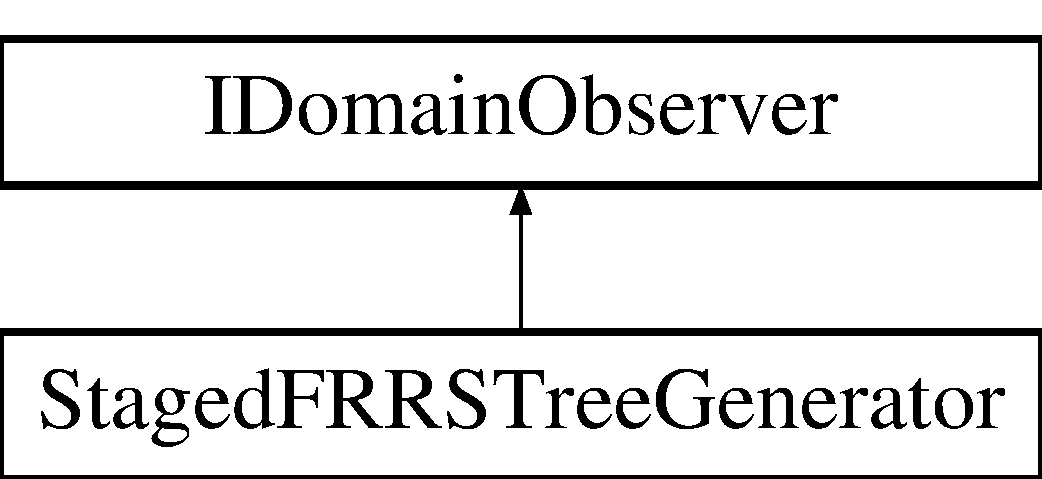
\includegraphics[height=2.000000cm]{d3/de1/class_staged_f_r_r_s_tree_generator}
\end{center}
\end{figure}
\subsection*{Public Member Functions}
\begin{DoxyCompactItemize}
\item 
\hyperlink{class_staged_f_r_r_s_tree_generator_a41ad2975c756af1dbbd3e59ebcdf458b}{Staged\+F\+R\+R\+S\+Tree\+Generator} (\hyperlink{class_staged_domain}{Staged\+Domain} $\ast$\hyperlink{class_staged_f_r_r_s_tree_generator_adc8ddbcf948810b70a7f9b59237a36e2}{domain}, \hyperlink{structpoint}{point} xi, double root\+Radii, double qi, long long int n\+Term, vector$<$ \hyperlink{class_abstract_constraint_function}{Abstract\+Constraint\+Function}$<$ double, int $>$ $\ast$ $>$gam, vector$<$ \hyperlink{class_abstract_constraint_function}{Abstract\+Constraint\+Function}$<$ double, int $>$ $\ast$ $>$eps\+Lim, vector$<$ \hyperlink{class_abstract_constraint_function}{Abstract\+Constraint\+Function}$<$ double, int $>$ $\ast$ $>$nu, double min\+Angle, double ref\+Pressure)
\item 
\hyperlink{class_staged_f_r_r_s_tree_generator_a69a07c273b05c768888c5691d393efc0}{Staged\+F\+R\+R\+S\+Tree\+Generator} (\hyperlink{class_staged_domain}{Staged\+Domain} $\ast$\hyperlink{class_staged_f_r_r_s_tree_generator_adc8ddbcf948810b70a7f9b59237a36e2}{domain}, \hyperlink{structpoint}{point} xi, double root\+Radii, double qi, long long int n\+Term, vector$<$ \hyperlink{class_abstract_constraint_function}{Abstract\+Constraint\+Function}$<$ double, int $>$ $\ast$ $>$gam, vector$<$ \hyperlink{class_abstract_constraint_function}{Abstract\+Constraint\+Function}$<$ double, int $>$ $\ast$ $>$eps\+Lim, vector$<$ \hyperlink{class_abstract_constraint_function}{Abstract\+Constraint\+Function}$<$ double, int $>$ $\ast$ $>$nu, double min\+Angle, double ref\+Pressure, double viscosity\+Tolerance, int optimized)
\item 
\hyperlink{class_staged_f_r_r_s_tree_generator_a6e558409d89c7ce682d98f217955ba77}{Staged\+F\+R\+R\+S\+Tree\+Generator} (\hyperlink{class_staged_domain}{Staged\+Domain} $\ast$\hyperlink{class_staged_f_r_r_s_tree_generator_adc8ddbcf948810b70a7f9b59237a36e2}{domain}, \hyperlink{class_abstract_structured_c_c_o_tree}{Abstract\+Structured\+C\+C\+O\+Tree} $\ast$\hyperlink{class_staged_f_r_r_s_tree_generator_a584a1e0e109ac6bdeae996178f8d8646}{tree}, long long int n\+Term, vector$<$ \hyperlink{class_abstract_constraint_function}{Abstract\+Constraint\+Function}$<$ double, int $>$ $\ast$ $>$gam, vector$<$ \hyperlink{class_abstract_constraint_function}{Abstract\+Constraint\+Function}$<$ double, int $>$ $\ast$ $>$eps\+Lim, vector$<$ \hyperlink{class_abstract_constraint_function}{Abstract\+Constraint\+Function}$<$ double, int $>$ $\ast$ $>$nu)
\item 
\hyperlink{class_abstract_structured_c_c_o_tree}{Abstract\+Structured\+C\+C\+O\+Tree} $\ast$ \hyperlink{class_staged_f_r_r_s_tree_generator_a86dde9bdc838234e1e88a52fdfd4c6c2}{generate} ()
\item 
\hyperlink{class_abstract_structured_c_c_o_tree}{Abstract\+Structured\+C\+C\+O\+Tree} $\ast$ \hyperlink{class_staged_f_r_r_s_tree_generator_a8a61382d3442b29f63f8b1cf5f3e8092}{resume} ()
\item 
\hyperlink{class_staged_domain}{Staged\+Domain} $\ast$ \hyperlink{class_staged_f_r_r_s_tree_generator_a3cc900c34c4324210a3e732d674e5ff0}{get\+Domain} ()
\item 
vector$<$ \hyperlink{class_abstract_structured_c_c_o_tree}{Abstract\+Structured\+C\+C\+O\+Tree} $\ast$ $>$ \hyperlink{class_staged_f_r_r_s_tree_generator_ac1296de9b742a6a0de36be4d094afd70}{get\+Trees} ()
\item 
void \hyperlink{class_staged_f_r_r_s_tree_generator_ac78a1dadc8a9eb640520d03d415db12b}{enable\+Configuration\+File} (string filename)
\item 
void \hyperlink{class_staged_f_r_r_s_tree_generator_a6f7629b00510e27edddced056e6fa1a1}{observable\+Modified} (\hyperlink{class_i_domain_observable}{I\+Domain\+Observable} $\ast$observable\+Instance)
\end{DoxyCompactItemize}
\subsection*{Protected Member Functions}
\begin{DoxyCompactItemize}
\item 
int \hyperlink{class_staged_f_r_r_s_tree_generator_aab108e277110635297d2d8cd95c4cd1d}{is\+Valid\+Root\+Segment} (\hyperlink{structpoint}{point} x\+New, int i\+Try)
\item 
int \hyperlink{class_staged_f_r_r_s_tree_generator_ac78cabfc8a80b398c4daa0d86a38f872}{is\+Valid\+Segment} (\hyperlink{structpoint}{point} x\+New, int i\+Try)
\item 
void \hyperlink{class_staged_f_r_r_s_tree_generator_aabba68aefd4f5786afa4460fdeb9519c}{generates\+Configuration\+File} (ios\+::openmode mode)
\item 
void \hyperlink{class_staged_f_r_r_s_tree_generator_a303c648e7d6d5df8e55c8263865be7e5}{mark\+Timestamp\+On\+Configuration\+File} (string label)
\item 
void \hyperlink{class_staged_f_r_r_s_tree_generator_acfdaf03eea5350e0fd2f59a5a76f6b23}{close\+Configuration\+File} ()
\end{DoxyCompactItemize}
\subsection*{Protected Attributes}
\begin{DoxyCompactItemize}
\item 
ofstream \hyperlink{class_staged_f_r_r_s_tree_generator_a764313586a157f7194ae945e76024e1f}{conf\+File}
\item 
chrono\+::steady\+\_\+clock\+::time\+\_\+point \hyperlink{class_staged_f_r_r_s_tree_generator_ae3f8c8407c40b6fac229574fcc8106d4}{beginning\+Time}
\end{DoxyCompactItemize}
\subsection*{Private Attributes}
\begin{DoxyCompactItemize}
\item 
\hyperlink{class_generator_data}{Generator\+Data} $\ast$ \hyperlink{class_staged_f_r_r_s_tree_generator_a8df19e56e9037a0f012cbaa6beb171ca}{instance\+Data}
\item 
\hyperlink{class_generator_data_monitor}{Generator\+Data\+Monitor} $\ast$ \hyperlink{class_staged_f_r_r_s_tree_generator_ad408787a8ec7350e68f00924ad6e8075}{data\+Monitor}
\item 
long long int \hyperlink{class_staged_f_r_r_s_tree_generator_a9ac1eafca6caa14601df23da77cfa565}{n\+Terminals}
\item 
double \hyperlink{class_staged_f_r_r_s_tree_generator_add278e195be9de240c8460e6480f0a44}{d\+Lim}
\item 
\hyperlink{class_staged_domain}{Staged\+Domain} $\ast$ \hyperlink{class_staged_f_r_r_s_tree_generator_adc8ddbcf948810b70a7f9b59237a36e2}{domain}
\item 
\hyperlink{class_abstract_structured_c_c_o_tree}{Abstract\+Structured\+C\+C\+O\+Tree} $\ast$ \hyperlink{class_staged_f_r_r_s_tree_generator_a584a1e0e109ac6bdeae996178f8d8646}{tree}
\item 
vector$<$ \hyperlink{class_abstract_constraint_function}{Abstract\+Constraint\+Function}$<$ double, int $>$ $\ast$ $>$ {\bfseries gams}\hypertarget{class_staged_f_r_r_s_tree_generator_a24e70672271f24d8a45d0a055202cb92}{}\label{class_staged_f_r_r_s_tree_generator_a24e70672271f24d8a45d0a055202cb92}

\item 
vector$<$ \hyperlink{class_abstract_constraint_function}{Abstract\+Constraint\+Function}$<$ double, int $>$ $\ast$ $>$ {\bfseries eps\+Lims}\hypertarget{class_staged_f_r_r_s_tree_generator_a40bf32899a1b6348a8808c8179074785}{}\label{class_staged_f_r_r_s_tree_generator_a40bf32899a1b6348a8808c8179074785}

\item 
vector$<$ \hyperlink{class_abstract_constraint_function}{Abstract\+Constraint\+Function}$<$ double, int $>$ $\ast$ $>$ {\bfseries nus}\hypertarget{class_staged_f_r_r_s_tree_generator_a8c5c7c43ff7483da4f2076debbf95217}{}\label{class_staged_f_r_r_s_tree_generator_a8c5c7c43ff7483da4f2076debbf95217}

\item 
int {\bfseries stage}\hypertarget{class_staged_f_r_r_s_tree_generator_a18fa6a223b79f35d001274c5fc9f8934}{}\label{class_staged_f_r_r_s_tree_generator_a18fa6a223b79f35d001274c5fc9f8934}

\item 
int \hyperlink{class_staged_f_r_r_s_tree_generator_ae6ab29d9d31103363d0f46e163f9e0cd}{is\+Generating\+Conf\+File}
\item 
string \hyperlink{class_staged_f_r_r_s_tree_generator_a051e558bc25271921834c40ff399a66b}{conf\+Filename}
\end{DoxyCompactItemize}


\subsection{Detailed Description}
Generator for a single fixed perfusion tree with many stages. 

\subsection{Constructor \& Destructor Documentation}
\index{Staged\+F\+R\+R\+S\+Tree\+Generator@{Staged\+F\+R\+R\+S\+Tree\+Generator}!Staged\+F\+R\+R\+S\+Tree\+Generator@{Staged\+F\+R\+R\+S\+Tree\+Generator}}
\index{Staged\+F\+R\+R\+S\+Tree\+Generator@{Staged\+F\+R\+R\+S\+Tree\+Generator}!Staged\+F\+R\+R\+S\+Tree\+Generator@{Staged\+F\+R\+R\+S\+Tree\+Generator}}
\subsubsection[{\texorpdfstring{Staged\+F\+R\+R\+S\+Tree\+Generator(\+Staged\+Domain $\ast$domain, point xi, double root\+Radii, double qi, long long int n\+Term, vector$<$ Abstract\+Constraint\+Function$<$ double, int $>$ $\ast$ $>$gam, vector$<$ Abstract\+Constraint\+Function$<$ double, int $>$ $\ast$ $>$eps\+Lim, vector$<$ Abstract\+Constraint\+Function$<$ double, int $>$ $\ast$ $>$nu, double min\+Angle, double ref\+Pressure)}{StagedFRRSTreeGenerator(StagedDomain *domain, point xi, double rootRadii, double qi, long long int nTerm, vector< AbstractConstraintFunction< double, int > * >gam, vector< AbstractConstraintFunction< double, int > * >epsLim, vector< AbstractConstraintFunction< double, int > * >nu, double minAngle, double refPressure)}}]{\setlength{\rightskip}{0pt plus 5cm}Staged\+F\+R\+R\+S\+Tree\+Generator\+::\+Staged\+F\+R\+R\+S\+Tree\+Generator (
\begin{DoxyParamCaption}
\item[{{\bf Staged\+Domain} $\ast$}]{domain, }
\item[{{\bf point}}]{xi, }
\item[{double}]{root\+Radii, }
\item[{double}]{qi, }
\item[{long long int}]{n\+Term, }
\item[{vector$<$ {\bf Abstract\+Constraint\+Function}$<$ double, int $>$ $\ast$ $>$}]{gam, }
\item[{vector$<$ {\bf Abstract\+Constraint\+Function}$<$ double, int $>$ $\ast$ $>$}]{eps\+Lim, }
\item[{vector$<$ {\bf Abstract\+Constraint\+Function}$<$ double, int $>$ $\ast$ $>$}]{nu, }
\item[{double}]{min\+Angle, }
\item[{double}]{ref\+Pressure}
\end{DoxyParamCaption}
)}\hypertarget{class_staged_f_r_r_s_tree_generator_a41ad2975c756af1dbbd3e59ebcdf458b}{}\label{class_staged_f_r_r_s_tree_generator_a41ad2975c756af1dbbd3e59ebcdf458b}
Constructor for non-\/optimized and constant viscosity tree. 
\begin{DoxyParams}{Parameters}
{\em domain} & Perfusion domain. \\
\hline
{\em xi} & Root proximal position. \\
\hline
{\em root\+Radii} & Root radius. \\
\hline
{\em qi} & Inflow for the perfusion domain. \\
\hline
{\em n\+Term} & Total number of tree terminals. \\
\hline
{\em gam} & Murray\textquotesingle{}s power law function. \\
\hline
{\em eps\+Lim} & Symmetry constraint function. \\
\hline
{\em nu} & Viscosity function. \\
\hline
{\em min\+Angle} & Minimum allowed bifurcation angle. \\
\hline
\end{DoxyParams}
\index{Staged\+F\+R\+R\+S\+Tree\+Generator@{Staged\+F\+R\+R\+S\+Tree\+Generator}!Staged\+F\+R\+R\+S\+Tree\+Generator@{Staged\+F\+R\+R\+S\+Tree\+Generator}}
\index{Staged\+F\+R\+R\+S\+Tree\+Generator@{Staged\+F\+R\+R\+S\+Tree\+Generator}!Staged\+F\+R\+R\+S\+Tree\+Generator@{Staged\+F\+R\+R\+S\+Tree\+Generator}}
\subsubsection[{\texorpdfstring{Staged\+F\+R\+R\+S\+Tree\+Generator(\+Staged\+Domain $\ast$domain, point xi, double root\+Radii, double qi, long long int n\+Term, vector$<$ Abstract\+Constraint\+Function$<$ double, int $>$ $\ast$ $>$gam, vector$<$ Abstract\+Constraint\+Function$<$ double, int $>$ $\ast$ $>$eps\+Lim, vector$<$ Abstract\+Constraint\+Function$<$ double, int $>$ $\ast$ $>$nu, double min\+Angle, double ref\+Pressure, double viscosity\+Tolerance, int optimized)}{StagedFRRSTreeGenerator(StagedDomain *domain, point xi, double rootRadii, double qi, long long int nTerm, vector< AbstractConstraintFunction< double, int > * >gam, vector< AbstractConstraintFunction< double, int > * >epsLim, vector< AbstractConstraintFunction< double, int > * >nu, double minAngle, double refPressure, double viscosityTolerance, int optimized)}}]{\setlength{\rightskip}{0pt plus 5cm}Staged\+F\+R\+R\+S\+Tree\+Generator\+::\+Staged\+F\+R\+R\+S\+Tree\+Generator (
\begin{DoxyParamCaption}
\item[{{\bf Staged\+Domain} $\ast$}]{domain, }
\item[{{\bf point}}]{xi, }
\item[{double}]{root\+Radii, }
\item[{double}]{qi, }
\item[{long long int}]{n\+Term, }
\item[{vector$<$ {\bf Abstract\+Constraint\+Function}$<$ double, int $>$ $\ast$ $>$}]{gam, }
\item[{vector$<$ {\bf Abstract\+Constraint\+Function}$<$ double, int $>$ $\ast$ $>$}]{eps\+Lim, }
\item[{vector$<$ {\bf Abstract\+Constraint\+Function}$<$ double, int $>$ $\ast$ $>$}]{nu, }
\item[{double}]{min\+Angle, }
\item[{double}]{ref\+Pressure, }
\item[{double}]{viscosity\+Tolerance, }
\item[{int}]{optimized}
\end{DoxyParamCaption}
)}\hypertarget{class_staged_f_r_r_s_tree_generator_a69a07c273b05c768888c5691d393efc0}{}\label{class_staged_f_r_r_s_tree_generator_a69a07c273b05c768888c5691d393efc0}
Constructor for tree with Fahraeus-\/\+Lindquist viscosity model. 
\begin{DoxyParams}{Parameters}
{\em domain} & Perfusion domain. \\
\hline
{\em xi} & Root proximal position. \\
\hline
{\em root\+Radii} & Root radius. \\
\hline
{\em qi} & Inflow for the perfusion domain. \\
\hline
{\em n\+Term} & Total number of tree terminals. \\
\hline
{\em gam} & Murray\textquotesingle{}s power law function. \\
\hline
{\em eps\+Lim} & Symmetry constraint function. \\
\hline
{\em nu} & Viscosity function. \\
\hline
{\em min\+Angle} & Minimum allowed bifurcation angle. \\
\hline
{\em viscosity\+Tolerance} & Convergence tolerance for the absolute beta variation in the viscosity iterative scheme. \\
\hline
{\em optimized} & If it is optimized with partial tree scaling. \\
\hline
\end{DoxyParams}
\index{Staged\+F\+R\+R\+S\+Tree\+Generator@{Staged\+F\+R\+R\+S\+Tree\+Generator}!Staged\+F\+R\+R\+S\+Tree\+Generator@{Staged\+F\+R\+R\+S\+Tree\+Generator}}
\index{Staged\+F\+R\+R\+S\+Tree\+Generator@{Staged\+F\+R\+R\+S\+Tree\+Generator}!Staged\+F\+R\+R\+S\+Tree\+Generator@{Staged\+F\+R\+R\+S\+Tree\+Generator}}
\subsubsection[{\texorpdfstring{Staged\+F\+R\+R\+S\+Tree\+Generator(\+Staged\+Domain $\ast$domain, Abstract\+Structured\+C\+C\+O\+Tree $\ast$tree, long long int n\+Term, vector$<$ Abstract\+Constraint\+Function$<$ double, int $>$ $\ast$ $>$gam, vector$<$ Abstract\+Constraint\+Function$<$ double, int $>$ $\ast$ $>$eps\+Lim, vector$<$ Abstract\+Constraint\+Function$<$ double, int $>$ $\ast$ $>$nu)}{StagedFRRSTreeGenerator(StagedDomain *domain, AbstractStructuredCCOTree *tree, long long int nTerm, vector< AbstractConstraintFunction< double, int > * >gam, vector< AbstractConstraintFunction< double, int > * >epsLim, vector< AbstractConstraintFunction< double, int > * >nu)}}]{\setlength{\rightskip}{0pt plus 5cm}Staged\+F\+R\+R\+S\+Tree\+Generator\+::\+Staged\+F\+R\+R\+S\+Tree\+Generator (
\begin{DoxyParamCaption}
\item[{{\bf Staged\+Domain} $\ast$}]{domain, }
\item[{{\bf Abstract\+Structured\+C\+C\+O\+Tree} $\ast$}]{tree, }
\item[{long long int}]{n\+Term, }
\item[{vector$<$ {\bf Abstract\+Constraint\+Function}$<$ double, int $>$ $\ast$ $>$}]{gam, }
\item[{vector$<$ {\bf Abstract\+Constraint\+Function}$<$ double, int $>$ $\ast$ $>$}]{eps\+Lim, }
\item[{vector$<$ {\bf Abstract\+Constraint\+Function}$<$ double, int $>$ $\ast$ $>$}]{nu}
\end{DoxyParamCaption}
)}\hypertarget{class_staged_f_r_r_s_tree_generator_a6e558409d89c7ce682d98f217955ba77}{}\label{class_staged_f_r_r_s_tree_generator_a6e558409d89c7ce682d98f217955ba77}
Constructor to resume from a pre-\/existent tree. 
\begin{DoxyParams}{Parameters}
{\em domain} & Perfusion domain. \\
\hline
{\em tree} & Pre-\/existent tree. \\
\hline
{\em n\+Term} & Total number of tree terminals. \\
\hline
{\em gam} & Murray\textquotesingle{}s power law function. \\
\hline
{\em eps\+Lim} & Symmetry constraint function. \\
\hline
{\em nu} & Viscosity function. \\
\hline
\end{DoxyParams}


\subsection{Member Function Documentation}
\index{Staged\+F\+R\+R\+S\+Tree\+Generator@{Staged\+F\+R\+R\+S\+Tree\+Generator}!close\+Configuration\+File@{close\+Configuration\+File}}
\index{close\+Configuration\+File@{close\+Configuration\+File}!Staged\+F\+R\+R\+S\+Tree\+Generator@{Staged\+F\+R\+R\+S\+Tree\+Generator}}
\subsubsection[{\texorpdfstring{close\+Configuration\+File()}{closeConfigurationFile()}}]{\setlength{\rightskip}{0pt plus 5cm}void Staged\+F\+R\+R\+S\+Tree\+Generator\+::close\+Configuration\+File (
\begin{DoxyParamCaption}
{}
\end{DoxyParamCaption}
)\hspace{0.3cm}{\ttfamily [protected]}}\hypertarget{class_staged_f_r_r_s_tree_generator_acfdaf03eea5350e0fd2f59a5a76f6b23}{}\label{class_staged_f_r_r_s_tree_generator_acfdaf03eea5350e0fd2f59a5a76f6b23}
Closes the configuration file for the current tree generation. \index{Staged\+F\+R\+R\+S\+Tree\+Generator@{Staged\+F\+R\+R\+S\+Tree\+Generator}!enable\+Configuration\+File@{enable\+Configuration\+File}}
\index{enable\+Configuration\+File@{enable\+Configuration\+File}!Staged\+F\+R\+R\+S\+Tree\+Generator@{Staged\+F\+R\+R\+S\+Tree\+Generator}}
\subsubsection[{\texorpdfstring{enable\+Configuration\+File(string filename)}{enableConfigurationFile(string filename)}}]{\setlength{\rightskip}{0pt plus 5cm}void Staged\+F\+R\+R\+S\+Tree\+Generator\+::enable\+Configuration\+File (
\begin{DoxyParamCaption}
\item[{string}]{filename}
\end{DoxyParamCaption}
)}\hypertarget{class_staged_f_r_r_s_tree_generator_ac78a1dadc8a9eb640520d03d415db12b}{}\label{class_staged_f_r_r_s_tree_generator_ac78a1dadc8a9eb640520d03d415db12b}
Enables the configuration file generation capabilities. 
\begin{DoxyParams}{Parameters}
{\em filename} & File name where the generator stores the configuration data. \\
\hline
\end{DoxyParams}
\index{Staged\+F\+R\+R\+S\+Tree\+Generator@{Staged\+F\+R\+R\+S\+Tree\+Generator}!generate@{generate}}
\index{generate@{generate}!Staged\+F\+R\+R\+S\+Tree\+Generator@{Staged\+F\+R\+R\+S\+Tree\+Generator}}
\subsubsection[{\texorpdfstring{generate()}{generate()}}]{\setlength{\rightskip}{0pt plus 5cm}{\bf Abstract\+Structured\+C\+C\+O\+Tree} $\ast$ Staged\+F\+R\+R\+S\+Tree\+Generator\+::generate (
\begin{DoxyParamCaption}
{}
\end{DoxyParamCaption}
)}\hypertarget{class_staged_f_r_r_s_tree_generator_a86dde9bdc838234e1e88a52fdfd4c6c2}{}\label{class_staged_f_r_r_s_tree_generator_a86dde9bdc838234e1e88a52fdfd4c6c2}
Generates the specified tree. \begin{DoxyReturn}{Returns}
Perfusion tree. 
\end{DoxyReturn}
\index{Staged\+F\+R\+R\+S\+Tree\+Generator@{Staged\+F\+R\+R\+S\+Tree\+Generator}!generates\+Configuration\+File@{generates\+Configuration\+File}}
\index{generates\+Configuration\+File@{generates\+Configuration\+File}!Staged\+F\+R\+R\+S\+Tree\+Generator@{Staged\+F\+R\+R\+S\+Tree\+Generator}}
\subsubsection[{\texorpdfstring{generates\+Configuration\+File(ios\+::openmode mode)}{generatesConfigurationFile(ios::openmode mode)}}]{\setlength{\rightskip}{0pt plus 5cm}void Staged\+F\+R\+R\+S\+Tree\+Generator\+::generates\+Configuration\+File (
\begin{DoxyParamCaption}
\item[{ios\+::openmode}]{mode}
\end{DoxyParamCaption}
)\hspace{0.3cm}{\ttfamily [protected]}}\hypertarget{class_staged_f_r_r_s_tree_generator_aabba68aefd4f5786afa4460fdeb9519c}{}\label{class_staged_f_r_r_s_tree_generator_aabba68aefd4f5786afa4460fdeb9519c}
Generates the configuration file for the current tree generation. 
\begin{DoxyParams}{Parameters}
{\em mode} & Is the openmode used for the generated file (ios\+::out for generation, ios\+::app for resume). \\
\hline
\end{DoxyParams}
\index{Staged\+F\+R\+R\+S\+Tree\+Generator@{Staged\+F\+R\+R\+S\+Tree\+Generator}!get\+Domain@{get\+Domain}}
\index{get\+Domain@{get\+Domain}!Staged\+F\+R\+R\+S\+Tree\+Generator@{Staged\+F\+R\+R\+S\+Tree\+Generator}}
\subsubsection[{\texorpdfstring{get\+Domain()}{getDomain()}}]{\setlength{\rightskip}{0pt plus 5cm}{\bf Staged\+Domain} $\ast$ Staged\+F\+R\+R\+S\+Tree\+Generator\+::get\+Domain (
\begin{DoxyParamCaption}
{}
\end{DoxyParamCaption}
)}\hypertarget{class_staged_f_r_r_s_tree_generator_a3cc900c34c4324210a3e732d674e5ff0}{}\label{class_staged_f_r_r_s_tree_generator_a3cc900c34c4324210a3e732d674e5ff0}
Returns the perfusion domain. \begin{DoxyReturn}{Returns}
Perfusion domain. 
\end{DoxyReturn}
\index{Staged\+F\+R\+R\+S\+Tree\+Generator@{Staged\+F\+R\+R\+S\+Tree\+Generator}!get\+Trees@{get\+Trees}}
\index{get\+Trees@{get\+Trees}!Staged\+F\+R\+R\+S\+Tree\+Generator@{Staged\+F\+R\+R\+S\+Tree\+Generator}}
\subsubsection[{\texorpdfstring{get\+Trees()}{getTrees()}}]{\setlength{\rightskip}{0pt plus 5cm}vector$<$ {\bf Abstract\+Structured\+C\+C\+O\+Tree} $\ast$ $>$ Staged\+F\+R\+R\+S\+Tree\+Generator\+::get\+Trees (
\begin{DoxyParamCaption}
{}
\end{DoxyParamCaption}
)}\hypertarget{class_staged_f_r_r_s_tree_generator_ac1296de9b742a6a0de36be4d094afd70}{}\label{class_staged_f_r_r_s_tree_generator_ac1296de9b742a6a0de36be4d094afd70}
Returns the generated tree. \begin{DoxyReturn}{Returns}
Generated tree. 
\end{DoxyReturn}
\index{Staged\+F\+R\+R\+S\+Tree\+Generator@{Staged\+F\+R\+R\+S\+Tree\+Generator}!is\+Valid\+Root\+Segment@{is\+Valid\+Root\+Segment}}
\index{is\+Valid\+Root\+Segment@{is\+Valid\+Root\+Segment}!Staged\+F\+R\+R\+S\+Tree\+Generator@{Staged\+F\+R\+R\+S\+Tree\+Generator}}
\subsubsection[{\texorpdfstring{is\+Valid\+Root\+Segment(point x\+New, int i\+Try)}{isValidRootSegment(point xNew, int iTry)}}]{\setlength{\rightskip}{0pt plus 5cm}int Staged\+F\+R\+R\+S\+Tree\+Generator\+::is\+Valid\+Root\+Segment (
\begin{DoxyParamCaption}
\item[{{\bf point}}]{x\+New, }
\item[{int}]{i\+Try}
\end{DoxyParamCaption}
)\hspace{0.3cm}{\ttfamily [protected]}}\hypertarget{class_staged_f_r_r_s_tree_generator_aab108e277110635297d2d8cd95c4cd1d}{}\label{class_staged_f_r_r_s_tree_generator_aab108e277110635297d2d8cd95c4cd1d}
Returns if the length of the segment defined by x\+Prox and x\+New is higher than d\+Lim (distance criterion). 
\begin{DoxyParams}{Parameters}
{\em x\+New} & Proposed distal point. \\
\hline
{\em i\+Try} & Number of trial. \\
\hline
\end{DoxyParams}
\begin{DoxyReturn}{Returns}
If the root segment is valid. 
\end{DoxyReturn}
\index{Staged\+F\+R\+R\+S\+Tree\+Generator@{Staged\+F\+R\+R\+S\+Tree\+Generator}!is\+Valid\+Segment@{is\+Valid\+Segment}}
\index{is\+Valid\+Segment@{is\+Valid\+Segment}!Staged\+F\+R\+R\+S\+Tree\+Generator@{Staged\+F\+R\+R\+S\+Tree\+Generator}}
\subsubsection[{\texorpdfstring{is\+Valid\+Segment(point x\+New, int i\+Try)}{isValidSegment(point xNew, int iTry)}}]{\setlength{\rightskip}{0pt plus 5cm}int Staged\+F\+R\+R\+S\+Tree\+Generator\+::is\+Valid\+Segment (
\begin{DoxyParamCaption}
\item[{{\bf point}}]{x\+New, }
\item[{int}]{i\+Try}
\end{DoxyParamCaption}
)\hspace{0.3cm}{\ttfamily [protected]}}\hypertarget{class_staged_f_r_r_s_tree_generator_ac78cabfc8a80b398c4daa0d86a38f872}{}\label{class_staged_f_r_r_s_tree_generator_ac78cabfc8a80b398c4daa0d86a38f872}
Returns if the closest point to the whole try is greater than d\+Lim (distance criterion for a new segment). 
\begin{DoxyParams}{Parameters}
{\em x\+New} & Proposed distal point. \\
\hline
{\em i\+Try} & Number of trial. \\
\hline
\end{DoxyParams}
\begin{DoxyReturn}{Returns}
If the segment is valid. 
\end{DoxyReturn}
\index{Staged\+F\+R\+R\+S\+Tree\+Generator@{Staged\+F\+R\+R\+S\+Tree\+Generator}!mark\+Timestamp\+On\+Configuration\+File@{mark\+Timestamp\+On\+Configuration\+File}}
\index{mark\+Timestamp\+On\+Configuration\+File@{mark\+Timestamp\+On\+Configuration\+File}!Staged\+F\+R\+R\+S\+Tree\+Generator@{Staged\+F\+R\+R\+S\+Tree\+Generator}}
\subsubsection[{\texorpdfstring{mark\+Timestamp\+On\+Configuration\+File(string label)}{markTimestampOnConfigurationFile(string label)}}]{\setlength{\rightskip}{0pt plus 5cm}void Staged\+F\+R\+R\+S\+Tree\+Generator\+::mark\+Timestamp\+On\+Configuration\+File (
\begin{DoxyParamCaption}
\item[{string}]{label}
\end{DoxyParamCaption}
)\hspace{0.3cm}{\ttfamily [protected]}}\hypertarget{class_staged_f_r_r_s_tree_generator_a303c648e7d6d5df8e55c8263865be7e5}{}\label{class_staged_f_r_r_s_tree_generator_a303c648e7d6d5df8e55c8263865be7e5}
Saves the timestamp for event {\ttfamily label}. \index{Staged\+F\+R\+R\+S\+Tree\+Generator@{Staged\+F\+R\+R\+S\+Tree\+Generator}!observable\+Modified@{observable\+Modified}}
\index{observable\+Modified@{observable\+Modified}!Staged\+F\+R\+R\+S\+Tree\+Generator@{Staged\+F\+R\+R\+S\+Tree\+Generator}}
\subsubsection[{\texorpdfstring{observable\+Modified(\+I\+Domain\+Observable $\ast$observable\+Instance)}{observableModified(IDomainObservable *observableInstance)}}]{\setlength{\rightskip}{0pt plus 5cm}void Staged\+F\+R\+R\+S\+Tree\+Generator\+::observable\+Modified (
\begin{DoxyParamCaption}
\item[{{\bf I\+Domain\+Observable} $\ast$}]{observable\+Instance}
\end{DoxyParamCaption}
)\hspace{0.3cm}{\ttfamily [virtual]}}\hypertarget{class_staged_f_r_r_s_tree_generator_a6f7629b00510e27edddced056e6fa1a1}{}\label{class_staged_f_r_r_s_tree_generator_a6f7629b00510e27edddced056e6fa1a1}
Updates internal data from this instance after the domain has been modified. 
\begin{DoxyParams}{Parameters}
{\em observable\+Instance} & Domain instance modified. \\
\hline
\end{DoxyParams}


Implements \hyperlink{class_i_domain_observer_aee18640c20a6feaa16e4bf3bdde887a3}{I\+Domain\+Observer}.

\index{Staged\+F\+R\+R\+S\+Tree\+Generator@{Staged\+F\+R\+R\+S\+Tree\+Generator}!resume@{resume}}
\index{resume@{resume}!Staged\+F\+R\+R\+S\+Tree\+Generator@{Staged\+F\+R\+R\+S\+Tree\+Generator}}
\subsubsection[{\texorpdfstring{resume()}{resume()}}]{\setlength{\rightskip}{0pt plus 5cm}{\bf Abstract\+Structured\+C\+C\+O\+Tree} $\ast$ Staged\+F\+R\+R\+S\+Tree\+Generator\+::resume (
\begin{DoxyParamCaption}
{}
\end{DoxyParamCaption}
)}\hypertarget{class_staged_f_r_r_s_tree_generator_a8a61382d3442b29f63f8b1cf5f3e8092}{}\label{class_staged_f_r_r_s_tree_generator_a8a61382d3442b29f63f8b1cf5f3e8092}
Resumes the tree generation. \begin{DoxyReturn}{Returns}
Perfusion tree. 
\end{DoxyReturn}


\subsection{Member Data Documentation}
\index{Staged\+F\+R\+R\+S\+Tree\+Generator@{Staged\+F\+R\+R\+S\+Tree\+Generator}!beginning\+Time@{beginning\+Time}}
\index{beginning\+Time@{beginning\+Time}!Staged\+F\+R\+R\+S\+Tree\+Generator@{Staged\+F\+R\+R\+S\+Tree\+Generator}}
\subsubsection[{\texorpdfstring{beginning\+Time}{beginningTime}}]{\setlength{\rightskip}{0pt plus 5cm}chrono\+::steady\+\_\+clock\+::time\+\_\+point Staged\+F\+R\+R\+S\+Tree\+Generator\+::beginning\+Time\hspace{0.3cm}{\ttfamily [protected]}}\hypertarget{class_staged_f_r_r_s_tree_generator_ae3f8c8407c40b6fac229574fcc8106d4}{}\label{class_staged_f_r_r_s_tree_generator_ae3f8c8407c40b6fac229574fcc8106d4}
Initial timestamp of the generation process. \index{Staged\+F\+R\+R\+S\+Tree\+Generator@{Staged\+F\+R\+R\+S\+Tree\+Generator}!conf\+File@{conf\+File}}
\index{conf\+File@{conf\+File}!Staged\+F\+R\+R\+S\+Tree\+Generator@{Staged\+F\+R\+R\+S\+Tree\+Generator}}
\subsubsection[{\texorpdfstring{conf\+File}{confFile}}]{\setlength{\rightskip}{0pt plus 5cm}ofstream Staged\+F\+R\+R\+S\+Tree\+Generator\+::conf\+File\hspace{0.3cm}{\ttfamily [protected]}}\hypertarget{class_staged_f_r_r_s_tree_generator_a764313586a157f7194ae945e76024e1f}{}\label{class_staged_f_r_r_s_tree_generator_a764313586a157f7194ae945e76024e1f}
Configuration file stream. \index{Staged\+F\+R\+R\+S\+Tree\+Generator@{Staged\+F\+R\+R\+S\+Tree\+Generator}!conf\+Filename@{conf\+Filename}}
\index{conf\+Filename@{conf\+Filename}!Staged\+F\+R\+R\+S\+Tree\+Generator@{Staged\+F\+R\+R\+S\+Tree\+Generator}}
\subsubsection[{\texorpdfstring{conf\+Filename}{confFilename}}]{\setlength{\rightskip}{0pt plus 5cm}string Staged\+F\+R\+R\+S\+Tree\+Generator\+::conf\+Filename\hspace{0.3cm}{\ttfamily [private]}}\hypertarget{class_staged_f_r_r_s_tree_generator_a051e558bc25271921834c40ff399a66b}{}\label{class_staged_f_r_r_s_tree_generator_a051e558bc25271921834c40ff399a66b}
File name for the configuration file. \index{Staged\+F\+R\+R\+S\+Tree\+Generator@{Staged\+F\+R\+R\+S\+Tree\+Generator}!data\+Monitor@{data\+Monitor}}
\index{data\+Monitor@{data\+Monitor}!Staged\+F\+R\+R\+S\+Tree\+Generator@{Staged\+F\+R\+R\+S\+Tree\+Generator}}
\subsubsection[{\texorpdfstring{data\+Monitor}{dataMonitor}}]{\setlength{\rightskip}{0pt plus 5cm}{\bf Generator\+Data\+Monitor}$\ast$ Staged\+F\+R\+R\+S\+Tree\+Generator\+::data\+Monitor\hspace{0.3cm}{\ttfamily [private]}}\hypertarget{class_staged_f_r_r_s_tree_generator_ad408787a8ec7350e68f00924ad6e8075}{}\label{class_staged_f_r_r_s_tree_generator_ad408787a8ec7350e68f00924ad6e8075}
Monitor of the {\ttfamily instance\+Data} . \index{Staged\+F\+R\+R\+S\+Tree\+Generator@{Staged\+F\+R\+R\+S\+Tree\+Generator}!d\+Lim@{d\+Lim}}
\index{d\+Lim@{d\+Lim}!Staged\+F\+R\+R\+S\+Tree\+Generator@{Staged\+F\+R\+R\+S\+Tree\+Generator}}
\subsubsection[{\texorpdfstring{d\+Lim}{dLim}}]{\setlength{\rightskip}{0pt plus 5cm}double Staged\+F\+R\+R\+S\+Tree\+Generator\+::d\+Lim\hspace{0.3cm}{\ttfamily [private]}}\hypertarget{class_staged_f_r_r_s_tree_generator_add278e195be9de240c8460e6480f0a44}{}\label{class_staged_f_r_r_s_tree_generator_add278e195be9de240c8460e6480f0a44}
Perfusion volume. \index{Staged\+F\+R\+R\+S\+Tree\+Generator@{Staged\+F\+R\+R\+S\+Tree\+Generator}!domain@{domain}}
\index{domain@{domain}!Staged\+F\+R\+R\+S\+Tree\+Generator@{Staged\+F\+R\+R\+S\+Tree\+Generator}}
\subsubsection[{\texorpdfstring{domain}{domain}}]{\setlength{\rightskip}{0pt plus 5cm}{\bf Staged\+Domain}$\ast$ Staged\+F\+R\+R\+S\+Tree\+Generator\+::domain\hspace{0.3cm}{\ttfamily [private]}}\hypertarget{class_staged_f_r_r_s_tree_generator_adc8ddbcf948810b70a7f9b59237a36e2}{}\label{class_staged_f_r_r_s_tree_generator_adc8ddbcf948810b70a7f9b59237a36e2}
Perfusion domain. \index{Staged\+F\+R\+R\+S\+Tree\+Generator@{Staged\+F\+R\+R\+S\+Tree\+Generator}!instance\+Data@{instance\+Data}}
\index{instance\+Data@{instance\+Data}!Staged\+F\+R\+R\+S\+Tree\+Generator@{Staged\+F\+R\+R\+S\+Tree\+Generator}}
\subsubsection[{\texorpdfstring{instance\+Data}{instanceData}}]{\setlength{\rightskip}{0pt plus 5cm}{\bf Generator\+Data}$\ast$ Staged\+F\+R\+R\+S\+Tree\+Generator\+::instance\+Data\hspace{0.3cm}{\ttfamily [private]}}\hypertarget{class_staged_f_r_r_s_tree_generator_a8df19e56e9037a0f012cbaa6beb171ca}{}\label{class_staged_f_r_r_s_tree_generator_a8df19e56e9037a0f012cbaa6beb171ca}
Wrapper with parameters associated to a tree generation process. \index{Staged\+F\+R\+R\+S\+Tree\+Generator@{Staged\+F\+R\+R\+S\+Tree\+Generator}!is\+Generating\+Conf\+File@{is\+Generating\+Conf\+File}}
\index{is\+Generating\+Conf\+File@{is\+Generating\+Conf\+File}!Staged\+F\+R\+R\+S\+Tree\+Generator@{Staged\+F\+R\+R\+S\+Tree\+Generator}}
\subsubsection[{\texorpdfstring{is\+Generating\+Conf\+File}{isGeneratingConfFile}}]{\setlength{\rightskip}{0pt plus 5cm}int Staged\+F\+R\+R\+S\+Tree\+Generator\+::is\+Generating\+Conf\+File\hspace{0.3cm}{\ttfamily [private]}}\hypertarget{class_staged_f_r_r_s_tree_generator_ae6ab29d9d31103363d0f46e163f9e0cd}{}\label{class_staged_f_r_r_s_tree_generator_ae6ab29d9d31103363d0f46e163f9e0cd}
If the current generation saves the configuration used. \index{Staged\+F\+R\+R\+S\+Tree\+Generator@{Staged\+F\+R\+R\+S\+Tree\+Generator}!n\+Terminals@{n\+Terminals}}
\index{n\+Terminals@{n\+Terminals}!Staged\+F\+R\+R\+S\+Tree\+Generator@{Staged\+F\+R\+R\+S\+Tree\+Generator}}
\subsubsection[{\texorpdfstring{n\+Terminals}{nTerminals}}]{\setlength{\rightskip}{0pt plus 5cm}long long int Staged\+F\+R\+R\+S\+Tree\+Generator\+::n\+Terminals\hspace{0.3cm}{\ttfamily [private]}}\hypertarget{class_staged_f_r_r_s_tree_generator_a9ac1eafca6caa14601df23da77cfa565}{}\label{class_staged_f_r_r_s_tree_generator_a9ac1eafca6caa14601df23da77cfa565}
Amount of terminals in the trees. \index{Staged\+F\+R\+R\+S\+Tree\+Generator@{Staged\+F\+R\+R\+S\+Tree\+Generator}!tree@{tree}}
\index{tree@{tree}!Staged\+F\+R\+R\+S\+Tree\+Generator@{Staged\+F\+R\+R\+S\+Tree\+Generator}}
\subsubsection[{\texorpdfstring{tree}{tree}}]{\setlength{\rightskip}{0pt plus 5cm}{\bf Abstract\+Structured\+C\+C\+O\+Tree}$\ast$ Staged\+F\+R\+R\+S\+Tree\+Generator\+::tree\hspace{0.3cm}{\ttfamily [private]}}\hypertarget{class_staged_f_r_r_s_tree_generator_a584a1e0e109ac6bdeae996178f8d8646}{}\label{class_staged_f_r_r_s_tree_generator_a584a1e0e109ac6bdeae996178f8d8646}
Generated trees. 

The documentation for this class was generated from the following files\+:\begin{DoxyCompactItemize}
\item 
core/Staged\+F\+R\+R\+S\+Tree\+Generator.\+h\item 
core/Staged\+F\+R\+R\+S\+Tree\+Generator.\+cpp\end{DoxyCompactItemize}

\hypertarget{class_std_stat_manipulator}{}\section{Std\+Stat\+Manipulator Class Reference}
\label{class_std_stat_manipulator}\index{Std\+Stat\+Manipulator@{Std\+Stat\+Manipulator}}


{\ttfamily \#include $<$Std\+Stat\+Manipulator.\+h$>$}

Inheritance diagram for Std\+Stat\+Manipulator\+:\begin{figure}[H]
\begin{center}
\leavevmode
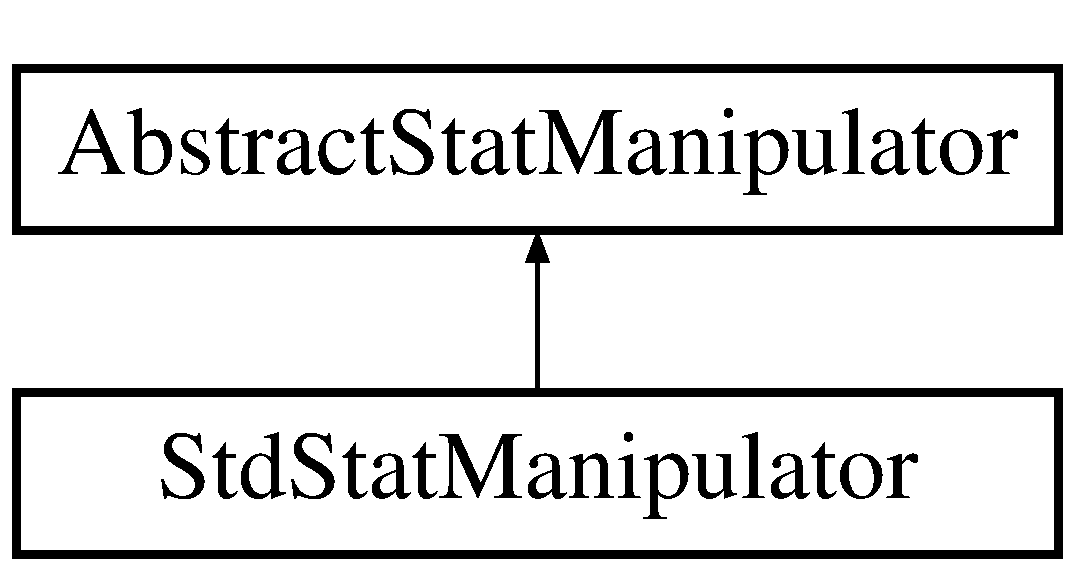
\includegraphics[height=2.000000cm]{d6/d5c/class_std_stat_manipulator}
\end{center}
\end{figure}
\subsection*{Public Member Functions}
\begin{DoxyCompactItemize}
\item 
\hyperlink{class_std_stat_manipulator_a9964b2c7f0912fec9f0671196594eafc}{Std\+Stat\+Manipulator} ()
\item 
double \hyperlink{class_std_stat_manipulator_a8b09c42b54d14322e805d153d8dfc028}{compute} (vector$<$ \hyperlink{structvessel}{vessel} $\ast$ $>$ vessels, \hyperlink{class_vessel_handler_a6cc775e9a5bcbe69ef381f56b52982e7}{Vessel\+Handler\+::\+A\+T\+T\+R\+I\+B\+U\+TE} att)
\end{DoxyCompactItemize}
\subsection*{Private Attributes}
\begin{DoxyCompactItemize}
\item 
\hyperlink{class_mean_stat_manipulator}{Mean\+Stat\+Manipulator} $\ast$ \hyperlink{class_std_stat_manipulator_aa14f0467d5a1ce40bfd78b3d39db54a1}{mean\+Manipulator}
\end{DoxyCompactItemize}
\subsection*{Additional Inherited Members}


\subsection{Detailed Description}
Computes the standard deviation value of a specific attribute for an array of vessels. 

\subsection{Constructor \& Destructor Documentation}
\index{Std\+Stat\+Manipulator@{Std\+Stat\+Manipulator}!Std\+Stat\+Manipulator@{Std\+Stat\+Manipulator}}
\index{Std\+Stat\+Manipulator@{Std\+Stat\+Manipulator}!Std\+Stat\+Manipulator@{Std\+Stat\+Manipulator}}
\subsubsection[{\texorpdfstring{Std\+Stat\+Manipulator()}{StdStatManipulator()}}]{\setlength{\rightskip}{0pt plus 5cm}Std\+Stat\+Manipulator\+::\+Std\+Stat\+Manipulator (
\begin{DoxyParamCaption}
{}
\end{DoxyParamCaption}
)}\hypertarget{class_std_stat_manipulator_a9964b2c7f0912fec9f0671196594eafc}{}\label{class_std_stat_manipulator_a9964b2c7f0912fec9f0671196594eafc}
Constructor. 

\subsection{Member Function Documentation}
\index{Std\+Stat\+Manipulator@{Std\+Stat\+Manipulator}!compute@{compute}}
\index{compute@{compute}!Std\+Stat\+Manipulator@{Std\+Stat\+Manipulator}}
\subsubsection[{\texorpdfstring{compute(vector$<$ vessel $\ast$ $>$ vessels, Vessel\+Handler\+::\+A\+T\+T\+R\+I\+B\+U\+T\+E att)}{compute(vector< vessel * > vessels, VesselHandler::ATTRIBUTE att)}}]{\setlength{\rightskip}{0pt plus 5cm}double Std\+Stat\+Manipulator\+::compute (
\begin{DoxyParamCaption}
\item[{vector$<$ {\bf vessel} $\ast$ $>$}]{vessels, }
\item[{{\bf Vessel\+Handler\+::\+A\+T\+T\+R\+I\+B\+U\+TE}}]{att}
\end{DoxyParamCaption}
)\hspace{0.3cm}{\ttfamily [virtual]}}\hypertarget{class_std_stat_manipulator_a8b09c42b54d14322e805d153d8dfc028}{}\label{class_std_stat_manipulator_a8b09c42b54d14322e805d153d8dfc028}
Computes the standard deviation of the attribute of interest among all {\ttfamily vessels}. 
\begin{DoxyParams}{Parameters}
{\em vessels} & Array of vessels from which the statistical function is computed. \\
\hline
\end{DoxyParams}
\begin{DoxyReturn}{Returns}
Standard deviation value. 
\end{DoxyReturn}


Implements \hyperlink{class_abstract_stat_manipulator_a8ae1dd190a2c85ff4e219a48f92763b7}{Abstract\+Stat\+Manipulator}.



\subsection{Member Data Documentation}
\index{Std\+Stat\+Manipulator@{Std\+Stat\+Manipulator}!mean\+Manipulator@{mean\+Manipulator}}
\index{mean\+Manipulator@{mean\+Manipulator}!Std\+Stat\+Manipulator@{Std\+Stat\+Manipulator}}
\subsubsection[{\texorpdfstring{mean\+Manipulator}{meanManipulator}}]{\setlength{\rightskip}{0pt plus 5cm}{\bf Mean\+Stat\+Manipulator}$\ast$ Std\+Stat\+Manipulator\+::mean\+Manipulator\hspace{0.3cm}{\ttfamily [private]}}\hypertarget{class_std_stat_manipulator_aa14f0467d5a1ce40bfd78b3d39db54a1}{}\label{class_std_stat_manipulator_aa14f0467d5a1ce40bfd78b3d39db54a1}
Mean statistical manipulator used to compute the mean internally. 

The documentation for this class was generated from the following files\+:\begin{DoxyCompactItemize}
\item 
stats/Std\+Stat\+Manipulator.\+h\item 
stats/Std\+Stat\+Manipulator.\+cpp\end{DoxyCompactItemize}

\hypertarget{class_tree_index_creator}{}\section{Tree\+Index\+Creator Class Reference}
\label{class_tree_index_creator}\index{Tree\+Index\+Creator@{Tree\+Index\+Creator}}


{\ttfamily \#include $<$Tree\+Index\+Creator.\+h$>$}

\subsection*{Public Member Functions}
\begin{DoxyCompactItemize}
\item 
\mbox{\hyperlink{class_tree_index_creator_ab8386c638c09069e53680e7461d76d5c}{Tree\+Index\+Creator}} (\mbox{\hyperlink{class_abstract_c_c_o_tree}{Abstract\+C\+C\+O\+Tree}} $\ast$tree)
\item 
\mbox{\Hypertarget{class_tree_index_creator_aaa96f17bfc82043b0ab3f78f9bdce9b5}\label{class_tree_index_creator_aaa96f17bfc82043b0ab3f78f9bdce9b5}} 
vector$<$ \mbox{\hyperlink{structvessel}{vessel}} $\ast$ $>$ {\bfseries get\+Terminals} ()
\item 
\mbox{\Hypertarget{class_tree_index_creator_aad7cac2dec20987a7099b1e62e5d89e9}\label{class_tree_index_creator_aad7cac2dec20987a7099b1e62e5d89e9}} 
vector$<$ \mbox{\hyperlink{structvessel}{vessel}} $\ast$ $>$ {\bfseries get\+All\+Segments} ()
\item 
\mbox{\Hypertarget{class_tree_index_creator_a19b04a2a699a2dc613c7a8c1aef204b9}\label{class_tree_index_creator_a19b04a2a699a2dc613c7a8c1aef204b9}} 
vector$<$ vector$<$ \mbox{\hyperlink{structvessel}{vessel}} $\ast$ $>$ $>$ {\bfseries get\+Segments\+By\+Level} ()
\end{DoxyCompactItemize}


\subsection{Detailed Description}
Creates indexes for a given tree to ease the manipulation of its segments. 

\subsection{Constructor \& Destructor Documentation}
\mbox{\Hypertarget{class_tree_index_creator_ab8386c638c09069e53680e7461d76d5c}\label{class_tree_index_creator_ab8386c638c09069e53680e7461d76d5c}} 
\index{Tree\+Index\+Creator@{Tree\+Index\+Creator}!Tree\+Index\+Creator@{Tree\+Index\+Creator}}
\index{Tree\+Index\+Creator@{Tree\+Index\+Creator}!Tree\+Index\+Creator@{Tree\+Index\+Creator}}
\subsubsection{\texorpdfstring{Tree\+Index\+Creator()}{TreeIndexCreator()}}
{\footnotesize\ttfamily Tree\+Index\+Creator\+::\+Tree\+Index\+Creator (\begin{DoxyParamCaption}\item[{\mbox{\hyperlink{class_abstract_c_c_o_tree}{Abstract\+C\+C\+O\+Tree}} $\ast$}]{tree }\end{DoxyParamCaption})}

Creates an instance associated with
\begin{DoxyParams}{Parameters}
{\em tree} & . \\
\hline
{\em tree} & Instance associated with the index creator. \\
\hline
\end{DoxyParams}


The documentation for this class was generated from the following files\+:\begin{DoxyCompactItemize}
\item 
stats/Tree\+Index\+Creator.\+h\item 
stats/Tree\+Index\+Creator.\+cpp\end{DoxyCompactItemize}

\hypertarget{class_tree_projector}{}\section{Tree\+Projector Class Reference}
\label{class_tree_projector}\index{Tree\+Projector@{Tree\+Projector}}


{\ttfamily \#include $<$Tree\+Projector.\+h$>$}

\subsection*{Public Member Functions}
\begin{DoxyCompactItemize}
\item 
\hyperlink{class_tree_projector_a8a2c3b716ebb81e1bfbe7cbfe65a84de}{Tree\+Projector} (string filename)
\item 
\hyperlink{class_tree_projector_ae40d424550e6551e1f772fe65d223e95}{Tree\+Projector} (string filename, double \hyperlink{class_tree_projector_ab6db6b968e5dc88efc732ef928e0dadc}{offset})
\item 
void \hyperlink{class_tree_projector_a7dc95446e85e5169d5777af5abbcd9a7}{project\+Terminals} (vector$<$ \hyperlink{class_single_vessel}{Single\+Vessel} $\ast$ $>$ vessels)
\item 
void {\bfseries project\+Vessel} (vector$<$ \hyperlink{class_single_vessel}{Single\+Vessel} $\ast$ $>$ vessels)\hypertarget{class_tree_projector_a98e0394085cbb9698587cee8636cf56f}{}\label{class_tree_projector_a98e0394085cbb9698587cee8636cf56f}

\end{DoxyCompactItemize}
\subsection*{Private Attributes}
\begin{DoxyCompactItemize}
\item 
vtk\+Smart\+Pointer$<$ vtk\+Poly\+Data $>$ \hyperlink{class_tree_projector_aca0dc09b8d4f959028f28e13f10d09f6}{vtk\+Geometry}
\item 
vtk\+Smart\+Pointer$<$ vtk\+Cell\+Locator $>$ \hyperlink{class_tree_projector_af67b13f1149ad2ee0b265b09fe4c7e4f}{locator}
\item 
double \hyperlink{class_tree_projector_ab6db6b968e5dc88efc732ef928e0dadc}{offset}
\end{DoxyCompactItemize}


\subsection{Detailed Description}
Projects a tree over or into a geometry. Mesh describing the geometry should have outgoing normals for the offset functionality. 

\subsection{Constructor \& Destructor Documentation}
\index{Tree\+Projector@{Tree\+Projector}!Tree\+Projector@{Tree\+Projector}}
\index{Tree\+Projector@{Tree\+Projector}!Tree\+Projector@{Tree\+Projector}}
\subsubsection[{\texorpdfstring{Tree\+Projector(string filename)}{TreeProjector(string filename)}}]{\setlength{\rightskip}{0pt plus 5cm}Tree\+Projector\+::\+Tree\+Projector (
\begin{DoxyParamCaption}
\item[{string}]{filename}
\end{DoxyParamCaption}
)}\hypertarget{class_tree_projector_a8a2c3b716ebb81e1bfbe7cbfe65a84de}{}\label{class_tree_projector_a8a2c3b716ebb81e1bfbe7cbfe65a84de}
Creates a projector associated to the geometrical domain described {\ttfamily filename}. 
\begin{DoxyParams}{Parameters}
{\em filename} & V\+TK file which contains the surface of the projection domain. \\
\hline
\end{DoxyParams}
\index{Tree\+Projector@{Tree\+Projector}!Tree\+Projector@{Tree\+Projector}}
\index{Tree\+Projector@{Tree\+Projector}!Tree\+Projector@{Tree\+Projector}}
\subsubsection[{\texorpdfstring{Tree\+Projector(string filename, double offset)}{TreeProjector(string filename, double offset)}}]{\setlength{\rightskip}{0pt plus 5cm}Tree\+Projector\+::\+Tree\+Projector (
\begin{DoxyParamCaption}
\item[{string}]{filename, }
\item[{double}]{offset}
\end{DoxyParamCaption}
)}\hypertarget{class_tree_projector_ae40d424550e6551e1f772fe65d223e95}{}\label{class_tree_projector_ae40d424550e6551e1f772fe65d223e95}
Creates a projector associated to the geometrical domain described {\ttfamily filename}. All projected points will be pushed inside 
\begin{DoxyParams}{Parameters}
{\em filename} & V\+TK file which contains the surface of the projection domain. \\
\hline
{\em offset} & \\
\hline
\end{DoxyParams}


\subsection{Member Function Documentation}
\index{Tree\+Projector@{Tree\+Projector}!project\+Terminals@{project\+Terminals}}
\index{project\+Terminals@{project\+Terminals}!Tree\+Projector@{Tree\+Projector}}
\subsubsection[{\texorpdfstring{project\+Terminals(vector$<$ Single\+Vessel $\ast$ $>$ vessels)}{projectTerminals(vector< SingleVessel * > vessels)}}]{\setlength{\rightskip}{0pt plus 5cm}void Tree\+Projector\+::project\+Terminals (
\begin{DoxyParamCaption}
\item[{vector$<$ {\bf Single\+Vessel} $\ast$ $>$}]{vessels}
\end{DoxyParamCaption}
)}\hypertarget{class_tree_projector_a7dc95446e85e5169d5777af5abbcd9a7}{}\label{class_tree_projector_a7dc95446e85e5169d5777af5abbcd9a7}
Projects the terminals of the vessels list to the closest point within the domain. 
\begin{DoxyParams}{Parameters}
{\em vessels} & \\
\hline
\end{DoxyParams}


\subsection{Member Data Documentation}
\index{Tree\+Projector@{Tree\+Projector}!locator@{locator}}
\index{locator@{locator}!Tree\+Projector@{Tree\+Projector}}
\subsubsection[{\texorpdfstring{locator}{locator}}]{\setlength{\rightskip}{0pt plus 5cm}vtk\+Smart\+Pointer$<$vtk\+Cell\+Locator$>$ Tree\+Projector\+::locator\hspace{0.3cm}{\ttfamily [private]}}\hypertarget{class_tree_projector_af67b13f1149ad2ee0b265b09fe4c7e4f}{}\label{class_tree_projector_af67b13f1149ad2ee0b265b09fe4c7e4f}
Cell locator responsible to determine if a segment is inside the domain. \index{Tree\+Projector@{Tree\+Projector}!offset@{offset}}
\index{offset@{offset}!Tree\+Projector@{Tree\+Projector}}
\subsubsection[{\texorpdfstring{offset}{offset}}]{\setlength{\rightskip}{0pt plus 5cm}double Tree\+Projector\+::offset\hspace{0.3cm}{\ttfamily [private]}}\hypertarget{class_tree_projector_ab6db6b968e5dc88efc732ef928e0dadc}{}\label{class_tree_projector_ab6db6b968e5dc88efc732ef928e0dadc}
Penetration offset for projected points \index{Tree\+Projector@{Tree\+Projector}!vtk\+Geometry@{vtk\+Geometry}}
\index{vtk\+Geometry@{vtk\+Geometry}!Tree\+Projector@{Tree\+Projector}}
\subsubsection[{\texorpdfstring{vtk\+Geometry}{vtkGeometry}}]{\setlength{\rightskip}{0pt plus 5cm}vtk\+Smart\+Pointer$<$vtk\+Poly\+Data$>$ Tree\+Projector\+::vtk\+Geometry\hspace{0.3cm}{\ttfamily [private]}}\hypertarget{class_tree_projector_aca0dc09b8d4f959028f28e13f10d09f6}{}\label{class_tree_projector_aca0dc09b8d4f959028f28e13f10d09f6}
vtk\+Polydata description of the domain. 

The documentation for this class was generated from the following files\+:\begin{DoxyCompactItemize}
\item 
structures/domain/Tree\+Projector.\+h\item 
structures/domain/Tree\+Projector.\+cpp\end{DoxyCompactItemize}

\hypertarget{class_tree_stats_manager}{}\section{Tree\+Stats\+Manager Class Reference}
\label{class_tree_stats_manager}\index{Tree\+Stats\+Manager@{Tree\+Stats\+Manager}}


{\ttfamily \#include $<$Tree\+Stats\+Manager.\+h$>$}

\subsection*{Public Member Functions}
\begin{DoxyCompactItemize}
\item 
{\bfseries Tree\+Stats\+Manager} (\hyperlink{class_abstract_structured_c_c_o_tree}{Abstract\+Structured\+C\+C\+O\+Tree} $\ast$\hyperlink{class_tree_stats_manager_a87781acaeb7b0eab470e6678c97b9ec5}{tree})\hypertarget{class_tree_stats_manager_a6073419bbbf25c7c9c37d7f7dd47c3fe}{}\label{class_tree_stats_manager_a6073419bbbf25c7c9c37d7f7dd47c3fe}

\item 
void \hyperlink{class_tree_stats_manager_a49a109dfc97178229e77fd1a79343423}{get\+Mean\+Per\+Level} (vector$<$ double $>$ $\ast$levels, vector$<$ double $>$ $\ast$means, vector$<$ double $>$ $\ast$stds, \hyperlink{class_vessel_handler_a6cc775e9a5bcbe69ef381f56b52982e7}{Vessel\+Handler\+::\+A\+T\+T\+R\+I\+B\+U\+TE} att)
\end{DoxyCompactItemize}
\subsection*{Private Attributes}
\begin{DoxyCompactItemize}
\item 
\hyperlink{class_abstract_structured_c_c_o_tree}{Abstract\+Structured\+C\+C\+O\+Tree} $\ast$ \hyperlink{class_tree_stats_manager_a87781acaeb7b0eab470e6678c97b9ec5}{tree}
\end{DoxyCompactItemize}


\subsection{Detailed Description}
Facade class used to access to all statistical analysis services implemented. The class aims to return vectors with the statistical results and no plots or any other outputs. Outputs are expected to be generated in the C\+C\+O\+Rendering library to decouple G\+UI from data and model components. The last is key to support the C\+CO library in clusters or environments with no G\+UI capabilities.

Creates an instance of the given {\ttfamily tree}. 
\begin{DoxyParams}{Parameters}
{\em tree} & Tree for statistical analysis. \\
\hline
\end{DoxyParams}


\subsection{Member Function Documentation}
\index{Tree\+Stats\+Manager@{Tree\+Stats\+Manager}!get\+Mean\+Per\+Level@{get\+Mean\+Per\+Level}}
\index{get\+Mean\+Per\+Level@{get\+Mean\+Per\+Level}!Tree\+Stats\+Manager@{Tree\+Stats\+Manager}}
\subsubsection[{\texorpdfstring{get\+Mean\+Per\+Level(vector$<$ double $>$ $\ast$levels, vector$<$ double $>$ $\ast$means, vector$<$ double $>$ $\ast$stds, Vessel\+Handler\+::\+A\+T\+T\+R\+I\+B\+U\+T\+E att)}{getMeanPerLevel(vector< double > *levels, vector< double > *means, vector< double > *stds, VesselHandler::ATTRIBUTE att)}}]{\setlength{\rightskip}{0pt plus 5cm}void Tree\+Stats\+Manager\+::get\+Mean\+Per\+Level (
\begin{DoxyParamCaption}
\item[{vector$<$ double $>$ $\ast$}]{levels, }
\item[{vector$<$ double $>$ $\ast$}]{means, }
\item[{vector$<$ double $>$ $\ast$}]{stds, }
\item[{{\bf Vessel\+Handler\+::\+A\+T\+T\+R\+I\+B\+U\+TE}}]{att}
\end{DoxyParamCaption}
)}\hypertarget{class_tree_stats_manager_a49a109dfc97178229e77fd1a79343423}{}\label{class_tree_stats_manager_a49a109dfc97178229e77fd1a79343423}
Load the vector {\ttfamily levels}, {\ttfamily means} and {\ttfamily stds} with the number of bifurcation level and mean and standard deviation of a vessel field across that levels. 
\begin{DoxyParams}{Parameters}
{\em levels} & Levels of bifurcation (0,..., N-\/1). \\
\hline
{\em means} & Mean for each level. \\
\hline
{\em stds} & Standard deviation for each level. \\
\hline
{\em att} & Field over which the mean and std is computed. \\
\hline
\end{DoxyParams}


\subsection{Member Data Documentation}
\index{Tree\+Stats\+Manager@{Tree\+Stats\+Manager}!tree@{tree}}
\index{tree@{tree}!Tree\+Stats\+Manager@{Tree\+Stats\+Manager}}
\subsubsection[{\texorpdfstring{tree}{tree}}]{\setlength{\rightskip}{0pt plus 5cm}{\bf Abstract\+Structured\+C\+C\+O\+Tree}$\ast$ Tree\+Stats\+Manager\+::tree\hspace{0.3cm}{\ttfamily [private]}}\hypertarget{class_tree_stats_manager_a87781acaeb7b0eab470e6678c97b9ec5}{}\label{class_tree_stats_manager_a87781acaeb7b0eab470e6678c97b9ec5}
Tree that undergo through statistical analysis. 

The documentation for this class was generated from the following files\+:\begin{DoxyCompactItemize}
\item 
stats/Tree\+Stats\+Manager.\+h\item 
stats/Tree\+Stats\+Manager.\+cpp\end{DoxyCompactItemize}

\hypertarget{class_uniform_distribution_generator}{}\section{Uniform\+Distribution\+Generator Class Reference}
\label{class_uniform_distribution_generator}\index{Uniform\+Distribution\+Generator@{Uniform\+Distribution\+Generator}}
Inheritance diagram for Uniform\+Distribution\+Generator\+:\begin{figure}[H]
\begin{center}
\leavevmode
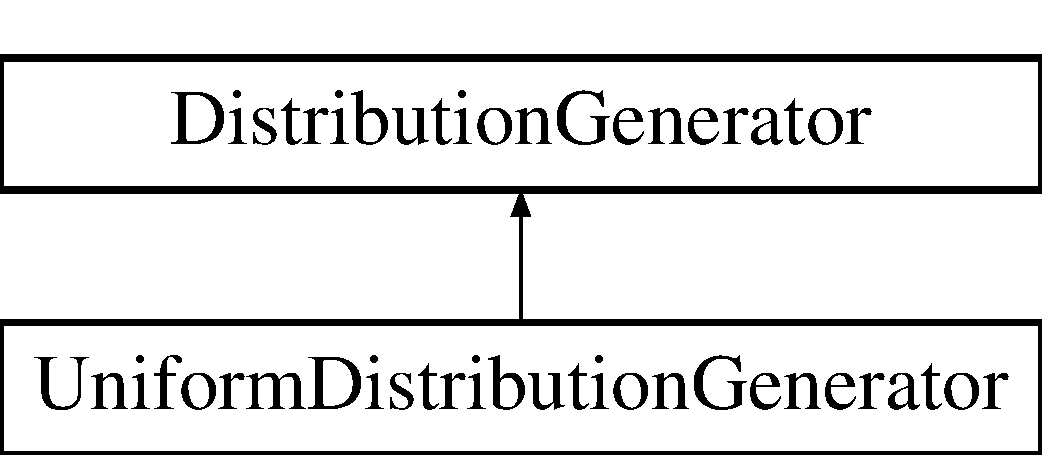
\includegraphics[height=2.000000cm]{db/d6b/class_uniform_distribution_generator}
\end{center}
\end{figure}
\subsection*{Public Member Functions}
\begin{DoxyCompactItemize}
\item 
\hyperlink{class_uniform_distribution_generator_ad736197918a5a3693b9f3dc820896ebb}{Uniform\+Distribution\+Generator} ()
\item 
virtual \hyperlink{class_uniform_distribution_generator_afa568e9c2fa1842b1e7aecd8dee8be85}{$\sim$\+Uniform\+Distribution\+Generator} ()
\item 
virtual void \hyperlink{class_uniform_distribution_generator_a9f40ba5dca7db03833f00a846218ae68}{initialize} (int seed, double $\ast$\hyperlink{class_distribution_generator_abbb670b1d48a4820559097b85bf6ee2d}{bounding\+Box})
\item 
vector$<$ \hyperlink{structpoint}{point} $>$ \hyperlink{class_uniform_distribution_generator_a3628de975c16748b69b5838e4b02ea41}{get\+N\+Points} (int n)
\end{DoxyCompactItemize}
\subsection*{Private Attributes}
\begin{DoxyCompactItemize}
\item 
uniform\+\_\+real\+\_\+distribution$<$ double $>$ \hyperlink{class_uniform_distribution_generator_a1e5c1a311993315dd08d2ef17e74e84d}{distX}
\item 
uniform\+\_\+real\+\_\+distribution$<$ double $>$ \hyperlink{class_uniform_distribution_generator_ada3c6906156a827e079a8085546a27c8}{distY}
\item 
uniform\+\_\+real\+\_\+distribution$<$ double $>$ \hyperlink{class_uniform_distribution_generator_ad5b89c08f50e76a4827af2e6eb9c5df8}{distZ}
\end{DoxyCompactItemize}
\subsection*{Additional Inherited Members}


\subsection{Constructor \& Destructor Documentation}
\index{Uniform\+Distribution\+Generator@{Uniform\+Distribution\+Generator}!Uniform\+Distribution\+Generator@{Uniform\+Distribution\+Generator}}
\index{Uniform\+Distribution\+Generator@{Uniform\+Distribution\+Generator}!Uniform\+Distribution\+Generator@{Uniform\+Distribution\+Generator}}
\subsubsection[{\texorpdfstring{Uniform\+Distribution\+Generator()}{UniformDistributionGenerator()}}]{\setlength{\rightskip}{0pt plus 5cm}Uniform\+Distribution\+Generator\+::\+Uniform\+Distribution\+Generator (
\begin{DoxyParamCaption}
{}
\end{DoxyParamCaption}
)}\hypertarget{class_uniform_distribution_generator_ad736197918a5a3693b9f3dc820896ebb}{}\label{class_uniform_distribution_generator_ad736197918a5a3693b9f3dc820896ebb}
Constructor. \index{Uniform\+Distribution\+Generator@{Uniform\+Distribution\+Generator}!````~Uniform\+Distribution\+Generator@{$\sim$\+Uniform\+Distribution\+Generator}}
\index{````~Uniform\+Distribution\+Generator@{$\sim$\+Uniform\+Distribution\+Generator}!Uniform\+Distribution\+Generator@{Uniform\+Distribution\+Generator}}
\subsubsection[{\texorpdfstring{$\sim$\+Uniform\+Distribution\+Generator()}{~UniformDistributionGenerator()}}]{\setlength{\rightskip}{0pt plus 5cm}Uniform\+Distribution\+Generator\+::$\sim$\+Uniform\+Distribution\+Generator (
\begin{DoxyParamCaption}
{}
\end{DoxyParamCaption}
)\hspace{0.3cm}{\ttfamily [virtual]}}\hypertarget{class_uniform_distribution_generator_afa568e9c2fa1842b1e7aecd8dee8be85}{}\label{class_uniform_distribution_generator_afa568e9c2fa1842b1e7aecd8dee8be85}
Destructor. 

\subsection{Member Function Documentation}
\index{Uniform\+Distribution\+Generator@{Uniform\+Distribution\+Generator}!get\+N\+Points@{get\+N\+Points}}
\index{get\+N\+Points@{get\+N\+Points}!Uniform\+Distribution\+Generator@{Uniform\+Distribution\+Generator}}
\subsubsection[{\texorpdfstring{get\+N\+Points(int n)}{getNPoints(int n)}}]{\setlength{\rightskip}{0pt plus 5cm}vector$<$ {\bf point} $>$ Uniform\+Distribution\+Generator\+::get\+N\+Points (
\begin{DoxyParamCaption}
\item[{int}]{n}
\end{DoxyParamCaption}
)\hspace{0.3cm}{\ttfamily [virtual]}}\hypertarget{class_uniform_distribution_generator_a3628de975c16748b69b5838e4b02ea41}{}\label{class_uniform_distribution_generator_a3628de975c16748b69b5838e4b02ea41}
Return a vector of {\ttfamily n} points of the distribution. 
\begin{DoxyParams}{Parameters}
{\em n} & Amount of output points. \\
\hline
\end{DoxyParams}
\begin{DoxyReturn}{Returns}
Vector of distribution points. 
\end{DoxyReturn}


Implements \hyperlink{class_distribution_generator_a777dcdfd3dee93cfcbcc00969f42ca29}{Distribution\+Generator}.

\index{Uniform\+Distribution\+Generator@{Uniform\+Distribution\+Generator}!initialize@{initialize}}
\index{initialize@{initialize}!Uniform\+Distribution\+Generator@{Uniform\+Distribution\+Generator}}
\subsubsection[{\texorpdfstring{initialize(int seed, double $\ast$bounding\+Box)}{initialize(int seed, double *boundingBox)}}]{\setlength{\rightskip}{0pt plus 5cm}void Uniform\+Distribution\+Generator\+::initialize (
\begin{DoxyParamCaption}
\item[{int}]{seed, }
\item[{double $\ast$}]{bounding\+Box}
\end{DoxyParamCaption}
)\hspace{0.3cm}{\ttfamily [virtual]}}\hypertarget{class_uniform_distribution_generator_a9f40ba5dca7db03833f00a846218ae68}{}\label{class_uniform_distribution_generator_a9f40ba5dca7db03833f00a846218ae68}
Initializer of the generator. Execute it before any getter call is performed. 

Reimplemented from \hyperlink{class_distribution_generator_ae4fa2d599942539e4b1971b0a8d5f8ba}{Distribution\+Generator}.



\subsection{Member Data Documentation}
\index{Uniform\+Distribution\+Generator@{Uniform\+Distribution\+Generator}!distX@{distX}}
\index{distX@{distX}!Uniform\+Distribution\+Generator@{Uniform\+Distribution\+Generator}}
\subsubsection[{\texorpdfstring{distX}{distX}}]{\setlength{\rightskip}{0pt plus 5cm}uniform\+\_\+real\+\_\+distribution$<$double$>$ Uniform\+Distribution\+Generator\+::distX\hspace{0.3cm}{\ttfamily [private]}}\hypertarget{class_uniform_distribution_generator_a1e5c1a311993315dd08d2ef17e74e84d}{}\label{class_uniform_distribution_generator_a1e5c1a311993315dd08d2ef17e74e84d}
Generator for X component \index{Uniform\+Distribution\+Generator@{Uniform\+Distribution\+Generator}!distY@{distY}}
\index{distY@{distY}!Uniform\+Distribution\+Generator@{Uniform\+Distribution\+Generator}}
\subsubsection[{\texorpdfstring{distY}{distY}}]{\setlength{\rightskip}{0pt plus 5cm}uniform\+\_\+real\+\_\+distribution$<$double$>$ Uniform\+Distribution\+Generator\+::distY\hspace{0.3cm}{\ttfamily [private]}}\hypertarget{class_uniform_distribution_generator_ada3c6906156a827e079a8085546a27c8}{}\label{class_uniform_distribution_generator_ada3c6906156a827e079a8085546a27c8}
Generator for Y component \index{Uniform\+Distribution\+Generator@{Uniform\+Distribution\+Generator}!distZ@{distZ}}
\index{distZ@{distZ}!Uniform\+Distribution\+Generator@{Uniform\+Distribution\+Generator}}
\subsubsection[{\texorpdfstring{distZ}{distZ}}]{\setlength{\rightskip}{0pt plus 5cm}uniform\+\_\+real\+\_\+distribution$<$double$>$ Uniform\+Distribution\+Generator\+::distZ\hspace{0.3cm}{\ttfamily [private]}}\hypertarget{class_uniform_distribution_generator_ad5b89c08f50e76a4827af2e6eb9c5df8}{}\label{class_uniform_distribution_generator_ad5b89c08f50e76a4827af2e6eb9c5df8}
Generator for Z component 

The documentation for this class was generated from the following files\+:\begin{DoxyCompactItemize}
\item 
structures/domain/Uniform\+Distribution\+Generator.\+h\item 
structures/domain/Uniform\+Distribution\+Generator.\+cpp\end{DoxyCompactItemize}

\hypertarget{structvessel}{}\section{vessel Struct Reference}
\label{structvessel}\index{vessel@{vessel}}
\subsection*{Public Attributes}
\begin{DoxyCompactItemize}
\item 
\mbox{\Hypertarget{structvessel_a621be11a4aabcc07863d07943060489e}\label{structvessel_a621be11a4aabcc07863d07943060489e}} 
vector$<$ \mbox{\hyperlink{structvessel}{vessel}} $\ast$ $>$ {\bfseries anastomose}
\item 
\mbox{\Hypertarget{structvessel_a94ada1fa10871eef938547df1267d66e}\label{structvessel_a94ada1fa10871eef938547df1267d66e}} 
vtk\+Smart\+Pointer$<$ vtk\+Line $>$ {\bfseries vtk\+Segment}
\item 
\mbox{\Hypertarget{structvessel_a5a44bb20222578bb67bf051164db7aad}\label{structvessel_a5a44bb20222578bb67bf051164db7aad}} 
vtk\+Id\+Type {\bfseries vtk\+Segment\+Id}
\item 
\mbox{\Hypertarget{structvessel_adc62693cc81142b471ec2aa525ba3bf5}\label{structvessel_adc62693cc81142b471ec2aa525ba3bf5}} 
\mbox{\hyperlink{structpoint}{point}} {\bfseries x\+Prox}
\item 
\mbox{\Hypertarget{structvessel_a0e84e9c1ccb9da3aea7145d63e803a30}\label{structvessel_a0e84e9c1ccb9da3aea7145d63e803a30}} 
\mbox{\hyperlink{structpoint}{point}} {\bfseries x\+Dist}
\item 
\mbox{\Hypertarget{structvessel_a40fb8bafbcd5654dc9bb48d49c97623a}\label{structvessel_a40fb8bafbcd5654dc9bb48d49c97623a}} 
int {\bfseries n\+Level}
\item 
\mbox{\Hypertarget{structvessel_a9bbe9528519d0df7931d2d3665ba45a6}\label{structvessel_a9bbe9528519d0df7931d2d3665ba45a6}} 
double {\bfseries radius}
\item 
\mbox{\Hypertarget{structvessel_a46380f25d12bee7300dfa5ad38ba9b38}\label{structvessel_a46380f25d12bee7300dfa5ad38ba9b38}} 
double {\bfseries beta}
\item 
\mbox{\Hypertarget{structvessel_a1336113e8af54e746e2b57ea4b4055d2}\label{structvessel_a1336113e8af54e746e2b57ea4b4055d2}} 
double {\bfseries length}
\item 
\mbox{\Hypertarget{structvessel_a86ef98b7df955a65573227a3cde46caf}\label{structvessel_a86ef98b7df955a65573227a3cde46caf}} 
double {\bfseries resistance}
\item 
\mbox{\Hypertarget{structvessel_a48f09ecdb7e15a0194a76a83c540c55a}\label{structvessel_a48f09ecdb7e15a0194a76a83c540c55a}} 
double {\bfseries flux}
\item 
\mbox{\Hypertarget{structvessel_a7f8917c9271c49f09d35f6d909ad313a}\label{structvessel_a7f8917c9271c49f09d35f6d909ad313a}} 
long int {\bfseries ID}
\item 
\mbox{\Hypertarget{structvessel_af3b90f07ee76daa83102037ce22a1b9e}\label{structvessel_af3b90f07ee76daa83102037ce22a1b9e}} 
double {\bfseries tree\+Volume}
\end{DoxyCompactItemize}


The documentation for this struct was generated from the following file\+:\begin{DoxyCompactItemize}
\item 
structures/C\+C\+O\+Common\+Structures.\+h\end{DoxyCompactItemize}

\hypertarget{class_vessel_filter_by_branching_mode}{}\section{Vessel\+Filter\+By\+Branching\+Mode Class Reference}
\label{class_vessel_filter_by_branching_mode}\index{Vessel\+Filter\+By\+Branching\+Mode@{Vessel\+Filter\+By\+Branching\+Mode}}
Inheritance diagram for Vessel\+Filter\+By\+Branching\+Mode\+:\begin{figure}[H]
\begin{center}
\leavevmode
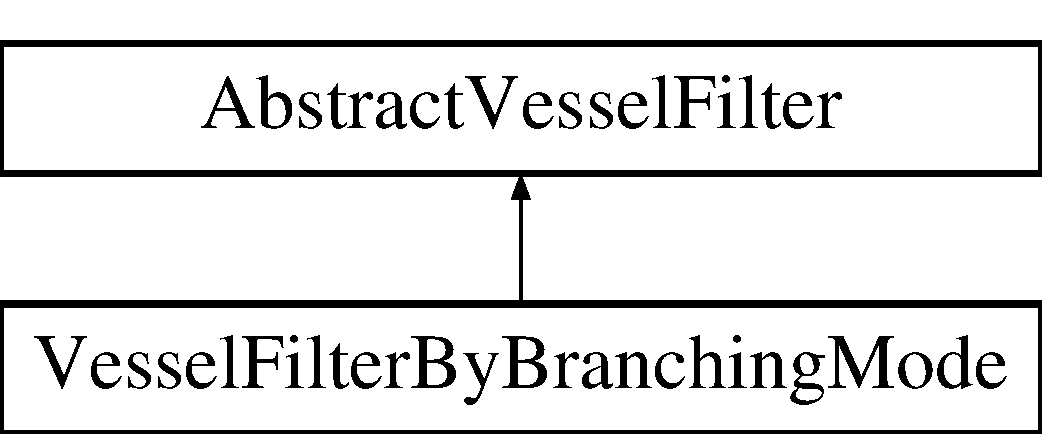
\includegraphics[height=2.000000cm]{d2/d26/class_vessel_filter_by_branching_mode}
\end{center}
\end{figure}
\subsection*{Public Member Functions}
\begin{DoxyCompactItemize}
\item 
{\bfseries Vessel\+Filter\+By\+Branching\+Mode} (\hyperlink{class_abstract_vascular_element_a2f7b3a097b944cd0b056fee00b93c860}{Abstract\+Vascular\+Element\+::\+B\+R\+A\+N\+C\+H\+I\+N\+G\+\_\+\+M\+O\+DE} mode)\hypertarget{class_vessel_filter_by_branching_mode_a161457b80ba91e39dce3ff3a426efedf}{}\label{class_vessel_filter_by_branching_mode_a161457b80ba91e39dce3ff3a426efedf}

\item 
vector$<$ \hyperlink{class_single_vessel}{Single\+Vessel} $\ast$ $>$ {\bfseries apply} (vector$<$ \hyperlink{class_single_vessel}{Single\+Vessel} $\ast$ $>$ vessels)\hypertarget{class_vessel_filter_by_branching_mode_a354fa634e3fdf886cc1be5e01910c926}{}\label{class_vessel_filter_by_branching_mode_a354fa634e3fdf886cc1be5e01910c926}

\end{DoxyCompactItemize}
\subsection*{Private Attributes}
\begin{DoxyCompactItemize}
\item 
\hyperlink{class_abstract_vascular_element_a2f7b3a097b944cd0b056fee00b93c860}{Abstract\+Vascular\+Element\+::\+B\+R\+A\+N\+C\+H\+I\+N\+G\+\_\+\+M\+O\+DE} {\bfseries mode}\hypertarget{class_vessel_filter_by_branching_mode_ae84a29f7425b260ce52fa1c6ab98654a}{}\label{class_vessel_filter_by_branching_mode_ae84a29f7425b260ce52fa1c6ab98654a}

\end{DoxyCompactItemize}


The documentation for this class was generated from the following files\+:\begin{DoxyCompactItemize}
\item 
filters/Vessel\+Filter\+By\+Branching\+Mode.\+h\item 
filters/Vessel\+Filter\+By\+Branching\+Mode.\+cpp\end{DoxyCompactItemize}

\hypertarget{class_vessel_filter_by_stage}{}\section{Vessel\+Filter\+By\+Stage Class Reference}
\label{class_vessel_filter_by_stage}\index{Vessel\+Filter\+By\+Stage@{Vessel\+Filter\+By\+Stage}}
Inheritance diagram for Vessel\+Filter\+By\+Stage\+:\begin{figure}[H]
\begin{center}
\leavevmode
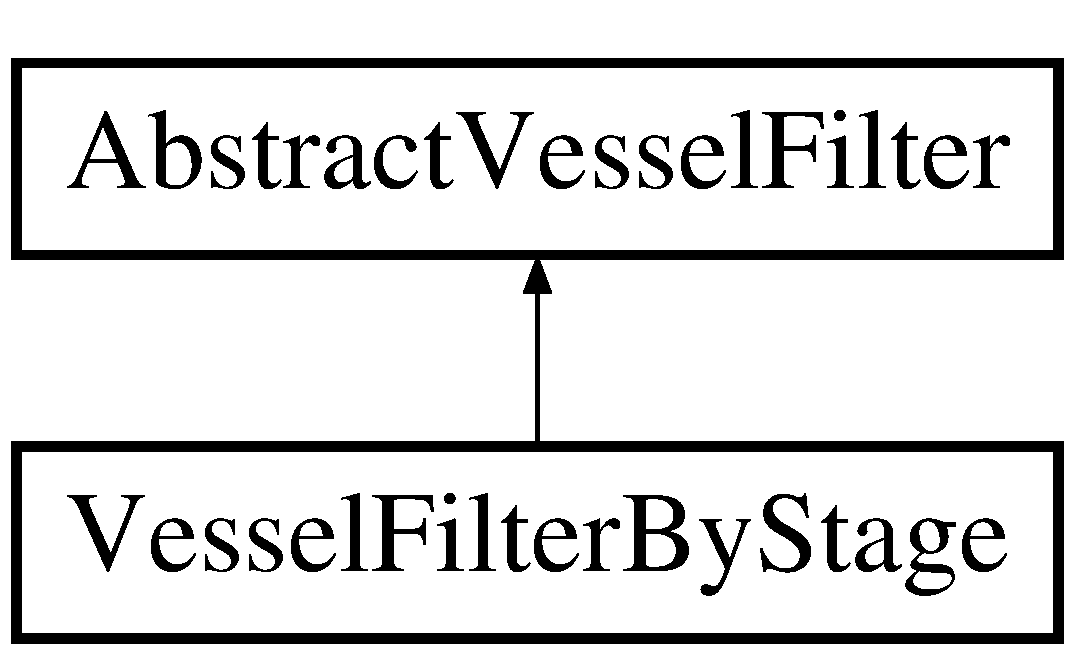
\includegraphics[height=2.000000cm]{dc/df0/class_vessel_filter_by_stage}
\end{center}
\end{figure}
\subsection*{Public Member Functions}
\begin{DoxyCompactItemize}
\item 
{\bfseries Vessel\+Filter\+By\+Stage} (int stage)\hypertarget{class_vessel_filter_by_stage_aa51b761ba5901792962fc598c73d68c3}{}\label{class_vessel_filter_by_stage_aa51b761ba5901792962fc598c73d68c3}

\item 
vector$<$ \hyperlink{class_single_vessel}{Single\+Vessel} $\ast$ $>$ {\bfseries apply} (vector$<$ \hyperlink{class_single_vessel}{Single\+Vessel} $\ast$ $>$ vessels)\hypertarget{class_vessel_filter_by_stage_a5445fc34bc3241dac1e844e394b88c55}{}\label{class_vessel_filter_by_stage_a5445fc34bc3241dac1e844e394b88c55}

\end{DoxyCompactItemize}
\subsection*{Private Attributes}
\begin{DoxyCompactItemize}
\item 
int {\bfseries stage}\hypertarget{class_vessel_filter_by_stage_abef7762212e101783828d06422aa3314}{}\label{class_vessel_filter_by_stage_abef7762212e101783828d06422aa3314}

\end{DoxyCompactItemize}


The documentation for this class was generated from the following files\+:\begin{DoxyCompactItemize}
\item 
filters/Vessel\+Filter\+By\+Stage.\+h\item 
filters/Vessel\+Filter\+By\+Stage.\+cpp\end{DoxyCompactItemize}

\hypertarget{class_vessel_filter_composite}{}\section{Vessel\+Filter\+Composite Class Reference}
\label{class_vessel_filter_composite}\index{Vessel\+Filter\+Composite@{Vessel\+Filter\+Composite}}


{\ttfamily \#include $<$Vessel\+Filter\+Composite.\+h$>$}

Inheritance diagram for Vessel\+Filter\+Composite\+:\begin{figure}[H]
\begin{center}
\leavevmode
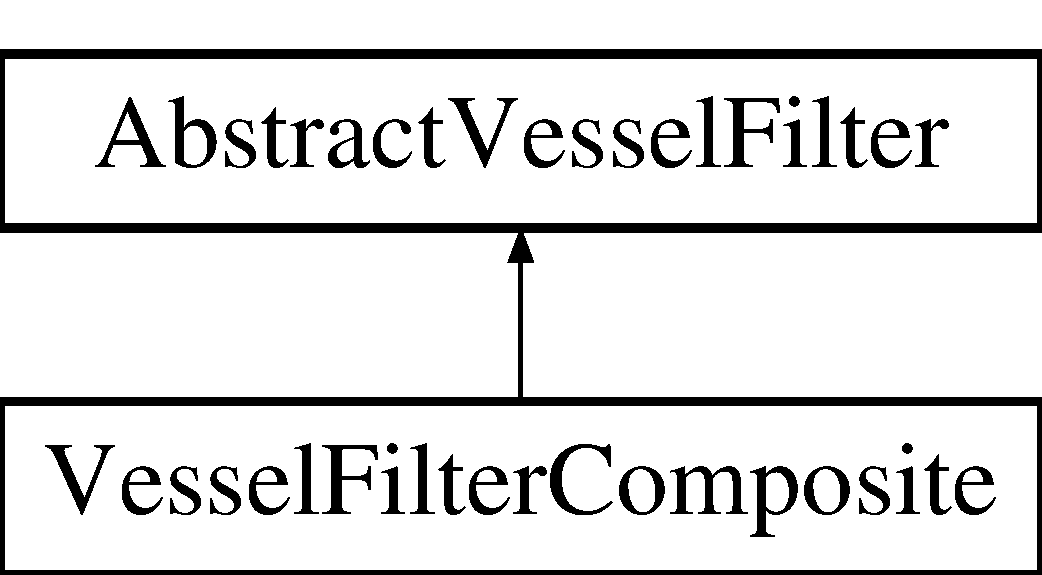
\includegraphics[height=2.000000cm]{d9/d3b/class_vessel_filter_composite}
\end{center}
\end{figure}
\subsection*{Public Member Functions}
\begin{DoxyCompactItemize}
\item 
{\bfseries Vessel\+Filter\+Composite} (vector$<$ \hyperlink{class_abstract_vessel_filter}{Abstract\+Vessel\+Filter} $\ast$ $>$ filters)\hypertarget{class_vessel_filter_composite_a5bc111a54d7cedcabb3bd84fec4b369b}{}\label{class_vessel_filter_composite_a5bc111a54d7cedcabb3bd84fec4b369b}

\item 
vector$<$ \hyperlink{class_single_vessel}{Single\+Vessel} $\ast$ $>$ {\bfseries apply} (vector$<$ \hyperlink{class_single_vessel}{Single\+Vessel} $\ast$ $>$ vessels)\hypertarget{class_vessel_filter_composite_a64cbf86a5abef6cb9cce717d38f50759}{}\label{class_vessel_filter_composite_a64cbf86a5abef6cb9cce717d38f50759}

\end{DoxyCompactItemize}
\subsection*{Private Attributes}
\begin{DoxyCompactItemize}
\item 
vector$<$ \hyperlink{class_abstract_vessel_filter}{Abstract\+Vessel\+Filter} $\ast$ $>$ {\bfseries filters}\hypertarget{class_vessel_filter_composite_ab5050a7510ed9d1a8d790ddfd906d102}{}\label{class_vessel_filter_composite_ab5050a7510ed9d1a8d790ddfd906d102}

\end{DoxyCompactItemize}


\subsection{Detailed Description}
Filters a set of vessels by a set of filters defined in the constructor. Implemented with Composite pattern. 

The documentation for this class was generated from the following files\+:\begin{DoxyCompactItemize}
\item 
filters/Vessel\+Filter\+Composite.\+h\item 
filters/Vessel\+Filter\+Composite.\+cpp\end{DoxyCompactItemize}

\hypertarget{class_vessel_handler}{}\section{Vessel\+Handler Class Reference}
\label{class_vessel_handler}\index{Vessel\+Handler@{Vessel\+Handler}}


{\ttfamily \#include $<$Vessel\+Handler.\+h$>$}

\subsection*{Public Types}
\begin{DoxyCompactItemize}
\item 
enum \hyperlink{class_vessel_handler_a6cc775e9a5bcbe69ef381f56b52982e7}{A\+T\+T\+R\+I\+B\+U\+TE} \{ \\*
{\bfseries D\+I\+A\+M\+E\+T\+ER}, 
{\bfseries R\+A\+D\+I\+US}, 
{\bfseries F\+L\+OW}, 
{\bfseries P\+R\+E\+S\+S\+U\+RE}, 
\\*
{\bfseries R\+E\+S\+I\+S\+T\+A\+N\+CE}, 
{\bfseries L\+E\+N\+G\+TH}, 
{\bfseries L\+E\+V\+EL}, 
{\bfseries B\+E\+TA}, 
\\*
{\bfseries V\+O\+L\+U\+ME}
 \}
\end{DoxyCompactItemize}
\subsection*{Public Member Functions}
\begin{DoxyCompactItemize}
\item 
\hyperlink{class_vessel_handler_afb4f79fe57971a6c27f70343bffe6104}{Vessel\+Handler} ()
\item 
double \hyperlink{class_vessel_handler_ab372d746a0206ef2660970d0666b7633}{get\+Vessel\+Attribute} (\hyperlink{structvessel}{vessel} $\ast$v, \hyperlink{class_vessel_handler_a6cc775e9a5bcbe69ef381f56b52982e7}{A\+T\+T\+R\+I\+B\+U\+TE} attribute)
\end{DoxyCompactItemize}


\subsection{Detailed Description}
Adapter class that allows data extraction from vessel structure by attribute in a dynamic manner. 

\subsection{Member Enumeration Documentation}
\index{Vessel\+Handler@{Vessel\+Handler}!A\+T\+T\+R\+I\+B\+U\+TE@{A\+T\+T\+R\+I\+B\+U\+TE}}
\index{A\+T\+T\+R\+I\+B\+U\+TE@{A\+T\+T\+R\+I\+B\+U\+TE}!Vessel\+Handler@{Vessel\+Handler}}
\subsubsection[{\texorpdfstring{A\+T\+T\+R\+I\+B\+U\+TE}{ATTRIBUTE}}]{\setlength{\rightskip}{0pt plus 5cm}enum {\bf Vessel\+Handler\+::\+A\+T\+T\+R\+I\+B\+U\+TE}}\hypertarget{class_vessel_handler_a6cc775e9a5bcbe69ef381f56b52982e7}{}\label{class_vessel_handler_a6cc775e9a5bcbe69ef381f56b52982e7}
Fields of vessel structure. 

\subsection{Constructor \& Destructor Documentation}
\index{Vessel\+Handler@{Vessel\+Handler}!Vessel\+Handler@{Vessel\+Handler}}
\index{Vessel\+Handler@{Vessel\+Handler}!Vessel\+Handler@{Vessel\+Handler}}
\subsubsection[{\texorpdfstring{Vessel\+Handler()}{VesselHandler()}}]{\setlength{\rightskip}{0pt plus 5cm}Vessel\+Handler\+::\+Vessel\+Handler (
\begin{DoxyParamCaption}
{}
\end{DoxyParamCaption}
)}\hypertarget{class_vessel_handler_afb4f79fe57971a6c27f70343bffe6104}{}\label{class_vessel_handler_afb4f79fe57971a6c27f70343bffe6104}
Dummy constructor. 

\subsection{Member Function Documentation}
\index{Vessel\+Handler@{Vessel\+Handler}!get\+Vessel\+Attribute@{get\+Vessel\+Attribute}}
\index{get\+Vessel\+Attribute@{get\+Vessel\+Attribute}!Vessel\+Handler@{Vessel\+Handler}}
\subsubsection[{\texorpdfstring{get\+Vessel\+Attribute(vessel $\ast$v, A\+T\+T\+R\+I\+B\+U\+T\+E attribute)}{getVesselAttribute(vessel *v, ATTRIBUTE attribute)}}]{\setlength{\rightskip}{0pt plus 5cm}double Vessel\+Handler\+::get\+Vessel\+Attribute (
\begin{DoxyParamCaption}
\item[{{\bf vessel} $\ast$}]{v, }
\item[{{\bf A\+T\+T\+R\+I\+B\+U\+TE}}]{attribute}
\end{DoxyParamCaption}
)}\hypertarget{class_vessel_handler_ab372d746a0206ef2660970d0666b7633}{}\label{class_vessel_handler_ab372d746a0206ef2660970d0666b7633}
Returns the specific {\ttfamily attribute} of the {\ttfamily v} vessel. 
\begin{DoxyParams}{Parameters}
{\em v} & Vessel of interest. \\
\hline
{\em attribute} & Field of interest. \\
\hline
\end{DoxyParams}
\begin{DoxyReturn}{Returns}
Value of the field {\ttfamily attribute} in vessel {\ttfamily v}. 
\end{DoxyReturn}


The documentation for this class was generated from the following files\+:\begin{DoxyCompactItemize}
\item 
stats/Vessel\+Handler.\+h\item 
stats/Vessel\+Handler.\+cpp\end{DoxyCompactItemize}

\hypertarget{class_visualization_saving_task}{}\section{Visualization\+Saving\+Task Class Reference}
\label{class_visualization_saving_task}\index{Visualization\+Saving\+Task@{Visualization\+Saving\+Task}}


{\ttfamily \#include $<$Visualization\+Saving\+Task.\+h$>$}

Inheritance diagram for Visualization\+Saving\+Task\+:\begin{figure}[H]
\begin{center}
\leavevmode
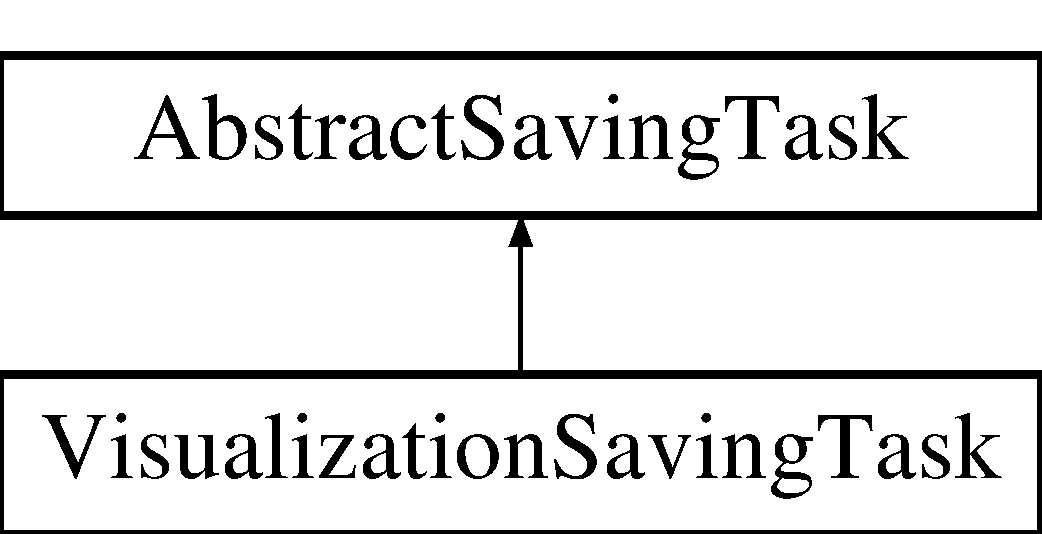
\includegraphics[height=2.000000cm]{df/d93/class_visualization_saving_task}
\end{center}
\end{figure}
\subsection*{Public Member Functions}
\begin{DoxyCompactItemize}
\item 
\hyperlink{class_visualization_saving_task_ab1b9318d4f8629a2d0f37355af3b9666}{Visualization\+Saving\+Task} (string path, string prefix, \hyperlink{class_abstract_object_c_c_o_tree}{Abstract\+Object\+C\+C\+O\+Tree} $\ast$tree)
\item 
void \hyperlink{class_visualization_saving_task_ac778c955205908fe4d5299b024fa2e6b}{execute} (long long int terminals)
\end{DoxyCompactItemize}
\subsection*{Private Attributes}
\begin{DoxyCompactItemize}
\item 
\hyperlink{class_abstract_object_c_c_o_tree}{Abstract\+Object\+C\+C\+O\+Tree} $\ast$ {\bfseries tree}\hypertarget{class_visualization_saving_task_adee46d7131ba48c77b94078be56eb0a9}{}\label{class_visualization_saving_task_adee46d7131ba48c77b94078be56eb0a9}

\item 
\hyperlink{class_v_t_k_object_tree_splines_nodal_writer}{V\+T\+K\+Object\+Tree\+Splines\+Nodal\+Writer} $\ast$ {\bfseries nodal\+Writer}\hypertarget{class_visualization_saving_task_ad84e3ab76408fb38372c274152f3fe10}{}\label{class_visualization_saving_task_ad84e3ab76408fb38372c274152f3fe10}

\item 
string {\bfseries path}\hypertarget{class_visualization_saving_task_afc36a4bf258c35bf97653dfd8e07bf29}{}\label{class_visualization_saving_task_afc36a4bf258c35bf97653dfd8e07bf29}

\item 
string {\bfseries prefix}\hypertarget{class_visualization_saving_task_a24bc1b701fcf209b4458f8fc5c988c10}{}\label{class_visualization_saving_task_a24bc1b701fcf209b4458f8fc5c988c10}

\end{DoxyCompactItemize}


\subsection{Detailed Description}
Saves the tree in .vtk format using splines to smooth the vessels. 

\subsection{Constructor \& Destructor Documentation}
\index{Visualization\+Saving\+Task@{Visualization\+Saving\+Task}!Visualization\+Saving\+Task@{Visualization\+Saving\+Task}}
\index{Visualization\+Saving\+Task@{Visualization\+Saving\+Task}!Visualization\+Saving\+Task@{Visualization\+Saving\+Task}}
\subsubsection[{\texorpdfstring{Visualization\+Saving\+Task(string path, string prefix, Abstract\+Object\+C\+C\+O\+Tree $\ast$tree)}{VisualizationSavingTask(string path, string prefix, AbstractObjectCCOTree *tree)}}]{\setlength{\rightskip}{0pt plus 5cm}Visualization\+Saving\+Task\+::\+Visualization\+Saving\+Task (
\begin{DoxyParamCaption}
\item[{string}]{path, }
\item[{string}]{prefix, }
\item[{{\bf Abstract\+Object\+C\+C\+O\+Tree} $\ast$}]{tree}
\end{DoxyParamCaption}
)}\hypertarget{class_visualization_saving_task_ab1b9318d4f8629a2d0f37355af3b9666}{}\label{class_visualization_saving_task_ab1b9318d4f8629a2d0f37355af3b9666}
Saves the {\ttfamily tree} in the given path. 
\begin{DoxyParams}{Parameters}
{\em path} & Output directory. \\
\hline
{\em prefix} & Prefix for the generated files. \\
\hline
{\em tree} & Tree to be stored in the generated files. \\
\hline
\end{DoxyParams}


\subsection{Member Function Documentation}
\index{Visualization\+Saving\+Task@{Visualization\+Saving\+Task}!execute@{execute}}
\index{execute@{execute}!Visualization\+Saving\+Task@{Visualization\+Saving\+Task}}
\subsubsection[{\texorpdfstring{execute(long long int terminals)}{execute(long long int terminals)}}]{\setlength{\rightskip}{0pt plus 5cm}void Visualization\+Saving\+Task\+::execute (
\begin{DoxyParamCaption}
\item[{long long int}]{terminals}
\end{DoxyParamCaption}
)\hspace{0.3cm}{\ttfamily [virtual]}}\hypertarget{class_visualization_saving_task_ac778c955205908fe4d5299b024fa2e6b}{}\label{class_visualization_saving_task_ac778c955205908fe4d5299b024fa2e6b}
Saves the tree in a visualization file using .vtk format. 

Implements \hyperlink{class_abstract_saving_task}{Abstract\+Saving\+Task}.



The documentation for this class was generated from the following files\+:\begin{DoxyCompactItemize}
\item 
io/task/Visualization\+Saving\+Task.\+h\item 
io/task/Visualization\+Saving\+Task.\+cpp\end{DoxyCompactItemize}

\hypertarget{class_volumetric_cost_estimator}{}\section{Volumetric\+Cost\+Estimator Class Reference}
\label{class_volumetric_cost_estimator}\index{Volumetric\+Cost\+Estimator@{Volumetric\+Cost\+Estimator}}


{\ttfamily \#include $<$Volumetric\+Cost\+Estimator.\+h$>$}

Inheritance diagram for Volumetric\+Cost\+Estimator\+:\begin{figure}[H]
\begin{center}
\leavevmode
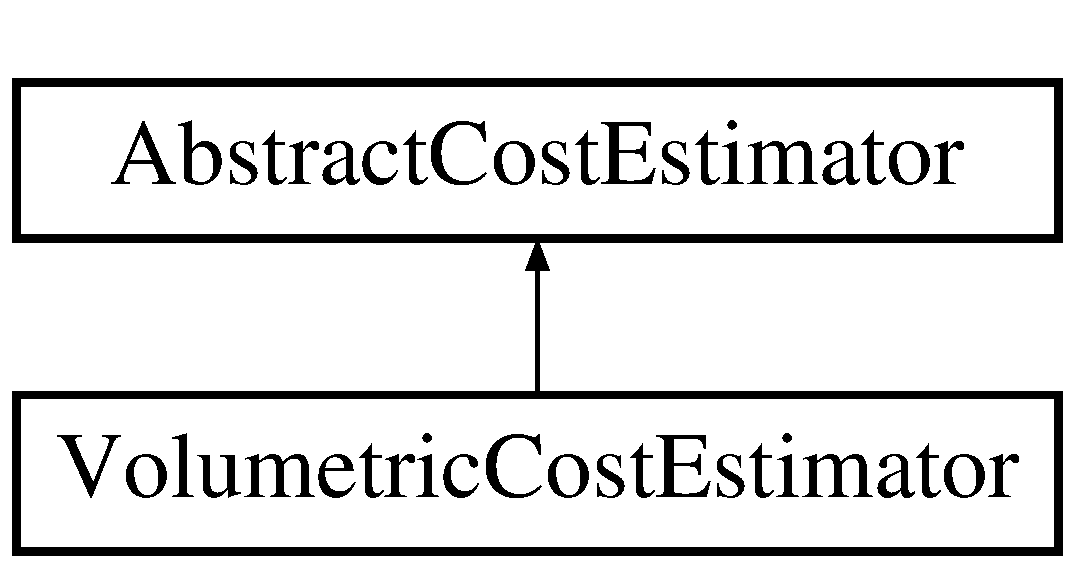
\includegraphics[height=2.000000cm]{d9/d3b/class_volumetric_cost_estimator}
\end{center}
\end{figure}
\subsection*{Public Member Functions}
\begin{DoxyCompactItemize}
\item 
\hyperlink{class_volumetric_cost_estimator_a1d3943123036c047a546bf9f8c55535a}{Volumetric\+Cost\+Estimator} ()
\item 
virtual \hyperlink{class_volumetric_cost_estimator_a5ef83e9f4192bc4e358dfdb61fd4418e}{$\sim$\+Volumetric\+Cost\+Estimator} ()
\item 
\hyperlink{class_abstract_cost_estimator}{Abstract\+Cost\+Estimator} $\ast$ \hyperlink{class_volumetric_cost_estimator_a513b5fa164962f2761485aebf44072bf}{clone} ()
\item 
void \hyperlink{class_volumetric_cost_estimator_a0ff762e6a26e1c6937cc28e88d1dc24d}{previous\+State} (\hyperlink{class_abstract_object_c_c_o_tree}{Abstract\+Object\+C\+C\+O\+Tree} $\ast$tree, \hyperlink{class_abstract_vascular_element}{Abstract\+Vascular\+Element} $\ast$parent, \hyperlink{structpoint}{point} i\+New, \hyperlink{structpoint}{point} i\+Test, double d\+Lim)
\item 
double \hyperlink{class_volumetric_cost_estimator_aca3637b77cc6657e4c5f916f09fd38e3}{compute\+Cost} (\hyperlink{class_abstract_object_c_c_o_tree}{Abstract\+Object\+C\+C\+O\+Tree} $\ast$tree)
\end{DoxyCompactItemize}
\subsection*{Private Member Functions}
\begin{DoxyCompactItemize}
\item 
double \hyperlink{class_volumetric_cost_estimator_a14ff0e932a5732dce0851e1279f42fb6}{compute\+Tree\+Cost} (\hyperlink{class_abstract_vascular_element}{Abstract\+Vascular\+Element} $\ast$root)
\end{DoxyCompactItemize}
\subsection*{Private Attributes}
\begin{DoxyCompactItemize}
\item 
double \hyperlink{class_volumetric_cost_estimator_a2671d960beddc83b44d1a8f65866e905}{previous\+Volume}
\end{DoxyCompactItemize}


\subsection{Detailed Description}
Cost estimator that computes the tree volume. 

\subsection{Constructor \& Destructor Documentation}
\index{Volumetric\+Cost\+Estimator@{Volumetric\+Cost\+Estimator}!Volumetric\+Cost\+Estimator@{Volumetric\+Cost\+Estimator}}
\index{Volumetric\+Cost\+Estimator@{Volumetric\+Cost\+Estimator}!Volumetric\+Cost\+Estimator@{Volumetric\+Cost\+Estimator}}
\subsubsection[{\texorpdfstring{Volumetric\+Cost\+Estimator()}{VolumetricCostEstimator()}}]{\setlength{\rightskip}{0pt plus 5cm}Volumetric\+Cost\+Estimator\+::\+Volumetric\+Cost\+Estimator (
\begin{DoxyParamCaption}
{}
\end{DoxyParamCaption}
)}\hypertarget{class_volumetric_cost_estimator_a1d3943123036c047a546bf9f8c55535a}{}\label{class_volumetric_cost_estimator_a1d3943123036c047a546bf9f8c55535a}
Common constructor. \index{Volumetric\+Cost\+Estimator@{Volumetric\+Cost\+Estimator}!````~Volumetric\+Cost\+Estimator@{$\sim$\+Volumetric\+Cost\+Estimator}}
\index{````~Volumetric\+Cost\+Estimator@{$\sim$\+Volumetric\+Cost\+Estimator}!Volumetric\+Cost\+Estimator@{Volumetric\+Cost\+Estimator}}
\subsubsection[{\texorpdfstring{$\sim$\+Volumetric\+Cost\+Estimator()}{~VolumetricCostEstimator()}}]{\setlength{\rightskip}{0pt plus 5cm}Volumetric\+Cost\+Estimator\+::$\sim$\+Volumetric\+Cost\+Estimator (
\begin{DoxyParamCaption}
{}
\end{DoxyParamCaption}
)\hspace{0.3cm}{\ttfamily [virtual]}}\hypertarget{class_volumetric_cost_estimator_a5ef83e9f4192bc4e358dfdb61fd4418e}{}\label{class_volumetric_cost_estimator_a5ef83e9f4192bc4e358dfdb61fd4418e}
Common destructor. 

\subsection{Member Function Documentation}
\index{Volumetric\+Cost\+Estimator@{Volumetric\+Cost\+Estimator}!clone@{clone}}
\index{clone@{clone}!Volumetric\+Cost\+Estimator@{Volumetric\+Cost\+Estimator}}
\subsubsection[{\texorpdfstring{clone()}{clone()}}]{\setlength{\rightskip}{0pt plus 5cm}{\bf Abstract\+Cost\+Estimator} $\ast$ Volumetric\+Cost\+Estimator\+::clone (
\begin{DoxyParamCaption}
{}
\end{DoxyParamCaption}
)\hspace{0.3cm}{\ttfamily [virtual]}}\hypertarget{class_volumetric_cost_estimator_a513b5fa164962f2761485aebf44072bf}{}\label{class_volumetric_cost_estimator_a513b5fa164962f2761485aebf44072bf}
Clones the current estimator instance. \begin{DoxyReturn}{Returns}
Cloned instance. 
\end{DoxyReturn}


Implements \hyperlink{class_abstract_cost_estimator_a928e53418b17eb68c443e2a68fe5cbcf}{Abstract\+Cost\+Estimator}.

\index{Volumetric\+Cost\+Estimator@{Volumetric\+Cost\+Estimator}!compute\+Cost@{compute\+Cost}}
\index{compute\+Cost@{compute\+Cost}!Volumetric\+Cost\+Estimator@{Volumetric\+Cost\+Estimator}}
\subsubsection[{\texorpdfstring{compute\+Cost(\+Abstract\+Object\+C\+C\+O\+Tree $\ast$tree)}{computeCost(AbstractObjectCCOTree *tree)}}]{\setlength{\rightskip}{0pt plus 5cm}double Volumetric\+Cost\+Estimator\+::compute\+Cost (
\begin{DoxyParamCaption}
\item[{{\bf Abstract\+Object\+C\+C\+O\+Tree} $\ast$}]{tree}
\end{DoxyParamCaption}
)\hspace{0.3cm}{\ttfamily [virtual]}}\hypertarget{class_volumetric_cost_estimator_aca3637b77cc6657e4c5f916f09fd38e3}{}\label{class_volumetric_cost_estimator_aca3637b77cc6657e4c5f916f09fd38e3}
Computes the functional cost of the given tree. 
\begin{DoxyParams}{Parameters}
{\em tree} & Tree at the current step. \\
\hline
\end{DoxyParams}
\begin{DoxyReturn}{Returns}
Cost of the given tree. 
\end{DoxyReturn}


Implements \hyperlink{class_abstract_cost_estimator_a2be0c6cc4aa6a73110c75ad903af428e}{Abstract\+Cost\+Estimator}.

\index{Volumetric\+Cost\+Estimator@{Volumetric\+Cost\+Estimator}!compute\+Tree\+Cost@{compute\+Tree\+Cost}}
\index{compute\+Tree\+Cost@{compute\+Tree\+Cost}!Volumetric\+Cost\+Estimator@{Volumetric\+Cost\+Estimator}}
\subsubsection[{\texorpdfstring{compute\+Tree\+Cost(\+Abstract\+Vascular\+Element $\ast$root)}{computeTreeCost(AbstractVascularElement *root)}}]{\setlength{\rightskip}{0pt plus 5cm}double Volumetric\+Cost\+Estimator\+::compute\+Tree\+Cost (
\begin{DoxyParamCaption}
\item[{{\bf Abstract\+Vascular\+Element} $\ast$}]{root}
\end{DoxyParamCaption}
)\hspace{0.3cm}{\ttfamily [private]}}\hypertarget{class_volumetric_cost_estimator_a14ff0e932a5732dce0851e1279f42fb6}{}\label{class_volumetric_cost_estimator_a14ff0e932a5732dce0851e1279f42fb6}
Computes the volume for the tree with root {\ttfamily root}. 
\begin{DoxyParams}{Parameters}
{\em root} & Root of the tree. \\
\hline
\end{DoxyParams}
\begin{DoxyReturn}{Returns}
Volume of the tree. 
\end{DoxyReturn}
\index{Volumetric\+Cost\+Estimator@{Volumetric\+Cost\+Estimator}!previous\+State@{previous\+State}}
\index{previous\+State@{previous\+State}!Volumetric\+Cost\+Estimator@{Volumetric\+Cost\+Estimator}}
\subsubsection[{\texorpdfstring{previous\+State(\+Abstract\+Object\+C\+C\+O\+Tree $\ast$tree, Abstract\+Vascular\+Element $\ast$parent, point i\+New, point i\+Test, double d\+Lim)}{previousState(AbstractObjectCCOTree *tree, AbstractVascularElement *parent, point iNew, point iTest, double dLim)}}]{\setlength{\rightskip}{0pt plus 5cm}void Volumetric\+Cost\+Estimator\+::previous\+State (
\begin{DoxyParamCaption}
\item[{{\bf Abstract\+Object\+C\+C\+O\+Tree} $\ast$}]{tree, }
\item[{{\bf Abstract\+Vascular\+Element} $\ast$}]{parent, }
\item[{{\bf point}}]{i\+New, }
\item[{{\bf point}}]{i\+Test, }
\item[{double}]{d\+Lim}
\end{DoxyParamCaption}
)\hspace{0.3cm}{\ttfamily [virtual]}}\hypertarget{class_volumetric_cost_estimator_a0ff762e6a26e1c6937cc28e88d1dc24d}{}\label{class_volumetric_cost_estimator_a0ff762e6a26e1c6937cc28e88d1dc24d}
Extracts information of the tree at the previous step. 
\begin{DoxyParams}{Parameters}
{\em root} & Root of the tree at the previous step. \\
\hline
{\em parent} & Vascular element where the new vessel will be connected. \\
\hline
{\em i\+New} & Distal position of the new vessel. \\
\hline
{\em i\+Test} & Proximal position of the new vessel. \\
\hline
{\em d\+Lim} & Minimum radius distance from the new vessel to the tree. \\
\hline
\end{DoxyParams}


Implements \hyperlink{class_abstract_cost_estimator_a8a806c3e4537c6d4acc428b029fd60de}{Abstract\+Cost\+Estimator}.



\subsection{Member Data Documentation}
\index{Volumetric\+Cost\+Estimator@{Volumetric\+Cost\+Estimator}!previous\+Volume@{previous\+Volume}}
\index{previous\+Volume@{previous\+Volume}!Volumetric\+Cost\+Estimator@{Volumetric\+Cost\+Estimator}}
\subsubsection[{\texorpdfstring{previous\+Volume}{previousVolume}}]{\setlength{\rightskip}{0pt plus 5cm}double Volumetric\+Cost\+Estimator\+::previous\+Volume\hspace{0.3cm}{\ttfamily [private]}}\hypertarget{class_volumetric_cost_estimator_a2671d960beddc83b44d1a8f65866e905}{}\label{class_volumetric_cost_estimator_a2671d960beddc83b44d1a8f65866e905}
Volume at the previous step. 

The documentation for this class was generated from the following files\+:\begin{DoxyCompactItemize}
\item 
structures/tree/Volumetric\+Cost\+Estimator.\+h\item 
structures/tree/Volumetric\+Cost\+Estimator.\+cpp\end{DoxyCompactItemize}

\hypertarget{class_v_t_k_converter}{}\section{V\+T\+K\+Converter Class Reference}
\label{class_v_t_k_converter}\index{V\+T\+K\+Converter@{V\+T\+K\+Converter}}


{\ttfamily \#include $<$V\+T\+K\+Converter.\+h$>$}

\subsection*{Static Public Member Functions}
\begin{DoxyCompactItemize}
\item 
static void \hyperlink{class_v_t_k_converter_aa3df2fb65ae80ec1ef476d9e00460cc6}{S\+T\+L2\+V\+T\+K\+Converter} (string stl\+File, string vtk\+File, int write\+A\+S\+C\+I\+I\+Format)
\item 
static void \hyperlink{class_v_t_k_converter_a060d99d6e878c421693ca47c73ecdcfc}{O\+B\+J2\+V\+T\+K\+Converter} (string obj\+File, string vtk\+File, int write\+A\+S\+C\+I\+I\+Format)
\end{DoxyCompactItemize}


\subsection{Detailed Description}
Converts different mesh formats to V\+TK using V\+TK library. 

\subsection{Member Function Documentation}
\index{V\+T\+K\+Converter@{V\+T\+K\+Converter}!O\+B\+J2\+V\+T\+K\+Converter@{O\+B\+J2\+V\+T\+K\+Converter}}
\index{O\+B\+J2\+V\+T\+K\+Converter@{O\+B\+J2\+V\+T\+K\+Converter}!V\+T\+K\+Converter@{V\+T\+K\+Converter}}
\subsubsection[{\texorpdfstring{O\+B\+J2\+V\+T\+K\+Converter(string obj\+File, string vtk\+File, int write\+A\+S\+C\+I\+I\+Format)}{OBJ2VTKConverter(string objFile, string vtkFile, int writeASCIIFormat)}}]{\setlength{\rightskip}{0pt plus 5cm}void V\+T\+K\+Converter\+::\+O\+B\+J2\+V\+T\+K\+Converter (
\begin{DoxyParamCaption}
\item[{string}]{obj\+File, }
\item[{string}]{vtk\+File, }
\item[{int}]{write\+A\+S\+C\+I\+I\+Format}
\end{DoxyParamCaption}
)\hspace{0.3cm}{\ttfamily [static]}}\hypertarget{class_v_t_k_converter_a060d99d6e878c421693ca47c73ecdcfc}{}\label{class_v_t_k_converter_a060d99d6e878c421693ca47c73ecdcfc}
Converts a mesh in O\+BJ format to V\+TK format. 
\begin{DoxyParams}{Parameters}
{\em obj\+File} & Input O\+BJ file. \\
\hline
{\em vtk\+File} & Output V\+TK file. \\
\hline
{\em write\+A\+S\+C\+I\+I\+Format} & True for A\+S\+C\+II V\+TK output, otherwise the output will be a binary V\+TK. \\
\hline
\end{DoxyParams}
\index{V\+T\+K\+Converter@{V\+T\+K\+Converter}!S\+T\+L2\+V\+T\+K\+Converter@{S\+T\+L2\+V\+T\+K\+Converter}}
\index{S\+T\+L2\+V\+T\+K\+Converter@{S\+T\+L2\+V\+T\+K\+Converter}!V\+T\+K\+Converter@{V\+T\+K\+Converter}}
\subsubsection[{\texorpdfstring{S\+T\+L2\+V\+T\+K\+Converter(string stl\+File, string vtk\+File, int write\+A\+S\+C\+I\+I\+Format)}{STL2VTKConverter(string stlFile, string vtkFile, int writeASCIIFormat)}}]{\setlength{\rightskip}{0pt plus 5cm}void V\+T\+K\+Converter\+::\+S\+T\+L2\+V\+T\+K\+Converter (
\begin{DoxyParamCaption}
\item[{string}]{stl\+File, }
\item[{string}]{vtk\+File, }
\item[{int}]{write\+A\+S\+C\+I\+I\+Format}
\end{DoxyParamCaption}
)\hspace{0.3cm}{\ttfamily [static]}}\hypertarget{class_v_t_k_converter_aa3df2fb65ae80ec1ef476d9e00460cc6}{}\label{class_v_t_k_converter_aa3df2fb65ae80ec1ef476d9e00460cc6}
Converts a mesh in S\+TL format to V\+TK format. 
\begin{DoxyParams}{Parameters}
{\em stl\+File} & Input S\+TL file. \\
\hline
{\em vtk\+File} & Output V\+TK file. \\
\hline
{\em write\+A\+S\+C\+I\+I\+Format} & True for A\+S\+C\+II V\+TK output, otherwise the output will be a binary V\+TK. \\
\hline
\end{DoxyParams}


The documentation for this class was generated from the following files\+:\begin{DoxyCompactItemize}
\item 
io/V\+T\+K\+Converter.\+h\item 
io/V\+T\+K\+Converter.\+cpp\end{DoxyCompactItemize}

\hypertarget{class_v_t_k_object_tree_elemental_writer}{}\section{V\+T\+K\+Object\+Tree\+Elemental\+Writer Class Reference}
\label{class_v_t_k_object_tree_elemental_writer}\index{V\+T\+K\+Object\+Tree\+Elemental\+Writer@{V\+T\+K\+Object\+Tree\+Elemental\+Writer}}
Inheritance diagram for V\+T\+K\+Object\+Tree\+Elemental\+Writer\+:\begin{figure}[H]
\begin{center}
\leavevmode
\includegraphics[height=2.000000cm]{dc/d27/class_v_t_k_object_tree_elemental_writer}
\end{center}
\end{figure}
\subsection*{Public Member Functions}
\begin{DoxyCompactItemize}
\item 
virtual void {\bfseries write} (string filename, \hyperlink{class_abstract_object_c_c_o_tree}{Abstract\+Object\+C\+C\+O\+Tree} $\ast$tree)\hypertarget{class_v_t_k_object_tree_elemental_writer_a23e1b460170169b56fe46923e134ec27}{}\label{class_v_t_k_object_tree_elemental_writer_a23e1b460170169b56fe46923e134ec27}

\end{DoxyCompactItemize}
\subsection*{Private Member Functions}
\begin{DoxyCompactItemize}
\item 
vector$<$ \hyperlink{class_single_vessel}{Single\+Vessel} $\ast$ $>$ \hyperlink{class_v_t_k_object_tree_elemental_writer_a79259a15da0c99f2851b468b0c90243e}{create\+V\+T\+K\+Index} (\hyperlink{class_abstract_object_c_c_o_tree}{Abstract\+Object\+C\+C\+O\+Tree} $\ast$tree)
\end{DoxyCompactItemize}


\subsection{Member Function Documentation}
\index{V\+T\+K\+Object\+Tree\+Elemental\+Writer@{V\+T\+K\+Object\+Tree\+Elemental\+Writer}!create\+V\+T\+K\+Index@{create\+V\+T\+K\+Index}}
\index{create\+V\+T\+K\+Index@{create\+V\+T\+K\+Index}!V\+T\+K\+Object\+Tree\+Elemental\+Writer@{V\+T\+K\+Object\+Tree\+Elemental\+Writer}}
\subsubsection[{\texorpdfstring{create\+V\+T\+K\+Index(\+Abstract\+Object\+C\+C\+O\+Tree $\ast$tree)}{createVTKIndex(AbstractObjectCCOTree *tree)}}]{\setlength{\rightskip}{0pt plus 5cm}vector$<$ {\bf Single\+Vessel} $\ast$ $>$ V\+T\+K\+Object\+Tree\+Elemental\+Writer\+::create\+V\+T\+K\+Index (
\begin{DoxyParamCaption}
\item[{{\bf Abstract\+Object\+C\+C\+O\+Tree} $\ast$}]{tree}
\end{DoxyParamCaption}
)\hspace{0.3cm}{\ttfamily [private]}}\hypertarget{class_v_t_k_object_tree_elemental_writer_a79259a15da0c99f2851b468b0c90243e}{}\label{class_v_t_k_object_tree_elemental_writer_a79259a15da0c99f2851b468b0c90243e}
Creates an ordered vector with all V\+TK identifiers of the vessels in the current tree. \begin{DoxyReturn}{Returns}
Vector with all V\+TK identifiers of the vessels in the current tree. 
\end{DoxyReturn}


The documentation for this class was generated from the following files\+:\begin{DoxyCompactItemize}
\item 
io/V\+T\+K\+Object\+Tree\+Elemental\+Writer.\+h\item 
io/V\+T\+K\+Object\+Tree\+Elemental\+Writer.\+cpp\end{DoxyCompactItemize}

\hypertarget{class_v_t_k_object_tree_nodal_writer}{}\section{V\+T\+K\+Object\+Tree\+Nodal\+Writer Class Reference}
\label{class_v_t_k_object_tree_nodal_writer}\index{V\+T\+K\+Object\+Tree\+Nodal\+Writer@{V\+T\+K\+Object\+Tree\+Nodal\+Writer}}
Inheritance diagram for V\+T\+K\+Object\+Tree\+Nodal\+Writer\+:\begin{figure}[H]
\begin{center}
\leavevmode
\includegraphics[height=2.000000cm]{df/d43/class_v_t_k_object_tree_nodal_writer}
\end{center}
\end{figure}
\subsection*{Public Member Functions}
\begin{DoxyCompactItemize}
\item 
virtual void {\bfseries write} (string filename, \hyperlink{class_abstract_object_c_c_o_tree}{Abstract\+Object\+C\+C\+O\+Tree} $\ast$tree)\hypertarget{class_v_t_k_object_tree_nodal_writer_ae468d7d7b2185e089d1574c311ceaebd}{}\label{class_v_t_k_object_tree_nodal_writer_ae468d7d7b2185e089d1574c311ceaebd}

\end{DoxyCompactItemize}


The documentation for this class was generated from the following files\+:\begin{DoxyCompactItemize}
\item 
io/V\+T\+K\+Object\+Tree\+Nodal\+Writer.\+h\item 
io/V\+T\+K\+Object\+Tree\+Nodal\+Writer.\+cpp\end{DoxyCompactItemize}

\hypertarget{class_v_t_k_object_tree_splines_nodal_writer}{}\section{V\+T\+K\+Object\+Tree\+Splines\+Nodal\+Writer Class Reference}
\label{class_v_t_k_object_tree_splines_nodal_writer}\index{V\+T\+K\+Object\+Tree\+Splines\+Nodal\+Writer@{V\+T\+K\+Object\+Tree\+Splines\+Nodal\+Writer}}
Inheritance diagram for V\+T\+K\+Object\+Tree\+Splines\+Nodal\+Writer\+:\begin{figure}[H]
\begin{center}
\leavevmode
\includegraphics[height=2.000000cm]{d3/d66/class_v_t_k_object_tree_splines_nodal_writer}
\end{center}
\end{figure}
\subsection*{Public Member Functions}
\begin{DoxyCompactItemize}
\item 
{\bfseries V\+T\+K\+Object\+Tree\+Splines\+Nodal\+Writer} (int resolution)\hypertarget{class_v_t_k_object_tree_splines_nodal_writer_a0b19d48b7adcfbe4f54636b0e6f66acd}{}\label{class_v_t_k_object_tree_splines_nodal_writer_a0b19d48b7adcfbe4f54636b0e6f66acd}

\item 
virtual void {\bfseries write} (string filename, \hyperlink{class_abstract_object_c_c_o_tree}{Abstract\+Object\+C\+C\+O\+Tree} $\ast$tree)\hypertarget{class_v_t_k_object_tree_splines_nodal_writer_a1c4404476233f13e8d778936b7e5b816}{}\label{class_v_t_k_object_tree_splines_nodal_writer_a1c4404476233f13e8d778936b7e5b816}

\end{DoxyCompactItemize}
\subsection*{Private Member Functions}
\begin{DoxyCompactItemize}
\item 
void {\bfseries compute\+Derivatives} (\hyperlink{class_single_vessel}{Single\+Vessel} $\ast$\hyperlink{structvessel}{vessel}, \hyperlink{structpoint}{point} \&proximal, \hyperlink{structpoint}{point} \&distal)\hypertarget{class_v_t_k_object_tree_splines_nodal_writer_ad8face2e1cf29239e57c3e7890ec5dc1}{}\label{class_v_t_k_object_tree_splines_nodal_writer_ad8face2e1cf29239e57c3e7890ec5dc1}

\end{DoxyCompactItemize}
\subsection*{Private Attributes}
\begin{DoxyCompactItemize}
\item 
int {\bfseries resolution}\hypertarget{class_v_t_k_object_tree_splines_nodal_writer_af12e22dc6d4affdcf8d3109d84774b01}{}\label{class_v_t_k_object_tree_splines_nodal_writer_af12e22dc6d4affdcf8d3109d84774b01}

\end{DoxyCompactItemize}


The documentation for this class was generated from the following files\+:\begin{DoxyCompactItemize}
\item 
io/V\+T\+K\+Object\+Tree\+Splines\+Nodal\+Writer.\+h\item 
io/V\+T\+K\+Object\+Tree\+Splines\+Nodal\+Writer.\+cpp\end{DoxyCompactItemize}

\hypertarget{class_v_t_k_object_tree_writer}{}\section{V\+T\+K\+Object\+Tree\+Writer Class Reference}
\label{class_v_t_k_object_tree_writer}\index{V\+T\+K\+Object\+Tree\+Writer@{V\+T\+K\+Object\+Tree\+Writer}}
Inheritance diagram for V\+T\+K\+Object\+Tree\+Writer\+:\begin{figure}[H]
\begin{center}
\leavevmode
\includegraphics[height=1.736434cm]{d0/d87/class_v_t_k_object_tree_writer}
\end{center}
\end{figure}
\subsection*{Public Member Functions}
\begin{DoxyCompactItemize}
\item 
virtual void {\bfseries write} (string filename, \hyperlink{class_abstract_object_c_c_o_tree}{Abstract\+Object\+C\+C\+O\+Tree} $\ast$tree)=0\hypertarget{class_v_t_k_object_tree_writer_ad4fb3ded12a62224613c0dc6fce8c610}{}\label{class_v_t_k_object_tree_writer_ad4fb3ded12a62224613c0dc6fce8c610}

\end{DoxyCompactItemize}


The documentation for this class was generated from the following files\+:\begin{DoxyCompactItemize}
\item 
io/V\+T\+K\+Object\+Tree\+Writer.\+h\item 
io/V\+T\+K\+Object\+Tree\+Writer.\+cpp\end{DoxyCompactItemize}

%--- End generated contents ---

% Index
\backmatter
\newpage
\phantomsection
\clearemptydoublepage
\addcontentsline{toc}{chapter}{Index}
\printindex

\end{document}
